\documentclass{beamer}
    \usepackage[utf8]{inputenc}
    \usepackage[T1]{fontenc}
    \usepackage[greek,english]{babel}
    \usepackage{bookmark}
    \usepackage{mathtools}
    \usepackage[compatibility,nofetsolderdot,nooldvoltagedirection,european,betterproportions]{circuitikz}
    \usepackage{tikz}
    \usepackage{pgf}
    \usepackage{pgfplots}
    \usepackage{listings}
    \usepackage{ifthen}
    \usepackage{algorithm}% http://ctan.org/pkg/algorithms
    \usepackage{algpseudocode}% http://ctan.org/pkg/algorithmicx

    \usetikzlibrary{positioning, arrows, patterns}

    \usetheme{Berlin}
    \setbeamertemplate{footline}{}
    \setbeamertemplate{headline}{}
    \setbeamertemplate{theorems}[ams style]
    \setbeamertemplate{caption}[numbered]
    % \setbeamercolor{normal text}{bg=gray!5}
    \usecolortheme{lily}
    \usefonttheme{professionalfonts}
    \beamertemplatenavigationsymbolsempty

    \title{Parallel-in-Time Integration in Circuit Simulation}
    \author[F. Madge]{Fabio Madge}
    % \institute{Technische Universität München}
    \date[24.09.19]{24. September 2019}

\begin{document}

    \maketitle

    \begin{frame}
    \setcounter{tocdepth}{1}
    \tableofcontents[pausesections]
    \end{frame}

    \AtBeginSection[]
    {
    \begin{frame}
    \setcounter{tocdepth}{2}
    \tableofcontents[currentsection,hideothersubsections]
    \end{frame}
    }

    \AtBeginSubsection[]
    {
    \begin{frame}
    \setcounter{tocdepth}{2}
    \tableofcontents[currentsection,
            currentsubsection,
            subsectionstyle=show/shaded/hide]
    \end{frame}
    }

    \section{Introduction}
    \subsection{Circuit Simulation}
\begin{frame}
\frametitle{Circuit}
\begin{figure}[ht]
    \centering\scalebox{1.5}{
        \begin{circuitikz}[scale=1.5]
            \draw (0,0) node[ground] {} to ++(0,1)
        -- ++(0,0) to[*R=$R$,a=$1\,\Omega$,-*] ++(2,0) node[above]{$u_1$}
        -- ++(0,0) to[*C=$C$,a=$100\,\mathrm{nF}$] ++(2,0)
        -- ++(0,0) to ++(0,-1) node[ground] {};
% \draw (3,0) to[R=1,i>_=1, o-*] (6,0);
        \end{circuitikz}}
    \caption{Loaded capacitor}
\label{fig:cap}
\end{figure}
Electric current \(I\)?
Electric potential \(V\)?
\end{frame}

\begin{frame}
\frametitle{Modified Nodal Analysis}
\begin{itemize}[<+->]
    \item Every element has a model
    \item Abstraction of the circuit as a graph \(G = (V,E)\)
    \item Kirchhoff's current law: \(\forall v \in V. \sum_{j \in E(v)} i_{j} = 0\)
\end{itemize}
\end{frame}

\begin{frame}
\frametitle{Example}
KCL: \(\forall v \in V. \sum_{j \in E(v)} i_{j} = 0\)
\begin{figure}[ht]
    \centering
        \begin{circuitikz}
            \draw (0,0) node[ground] {} to ++(0,1)
        -- ++(0,0) to[*R=$R$,a=$1\,\Omega$,-*] ++(2,0) node[above]{$u_1$}
        -- ++(0,0) to[*C=$C$,a=$100\,\mathrm{nF}$] ++(2,0)
        -- ++(0,0) to ++(0,-1) node[ground] {};
% \draw (3,0) to[R=1,i>_=1, o-*] (6,0);
        \end{circuitikz}
    \caption{Loaded capacitor}
\label{fig:cap}
\end{figure}
\pause
\begin{enumerate}[<+->]
    \item \(C\dot{u}_1 + Gu_1 = 0,\quad G=\frac{1}{R}\) (Conductance)
    \item \(C \dot{x} + G x = s(t)\)
    \item \(C (\alpha x + \beta) + G x = s(t)\)
    \item \(C (\alpha x + \beta) + G x - s(t)= 0\)
\end{enumerate}
\end{frame}


\subsection{Parallel Numerical Integration}
\begin{frame}
\frametitle{Problem: Inital Value Problem}
\begin{equation*}
y'(t) = f(t,y(t)), \quad y(t_0) = y_0.
\end{equation*}
\end{frame}

\begin{frame}
\frametitle{Solution*: Implicit Euler}
\begin{equation*}
y_{n+1} = y_n + hf(t_n,y_n)
\end{equation*}
\end{frame}



    \section{Algorithm: Parareal}
    \begin{frame}
    \frametitle{Idea of the Parareal Algorithm}
    \begin{itemize}[<+->]
        \item Introduced by Lions\footfullcite{Lions:2001}. More approachable\footfullcite{Gander:2015}.
        \item Parallel-in-time: Decomposition of \(\left(t_0, T\right] = \bigcup_{i=0}^{P-1} \left(t_i, t_{i+1}\right]\)
        \item Solve the subintervals in parallel
        \item Combination of coarse \(\mathcal{G}\) (fast) and fine \(\mathcal{F}\) (accurate) solver
        \item Run them over multiple iterations
        \item Start with \(\mathcal{G}\!\left(y, t_{A}, t_{\Omega}\right)\) for initial value:\\\(y_{j}^{0} = \mathcal{G}\!\left(y(t_0), t_0, t_{j}\right), \quad j \in \left\{i \,\middle|\, 0 \leq i < P\right\}\)
        \begin{scriptsize}
        \begin{description}[\(t_{A}\)]
            \item[\(y\)]<.-> Initial value
            \item[\(t_{A}\)]<.-> Start time of simulation
            \item[\(t_{\Omega}\)]<.-> End time of simulation
        \end{description}
        \end{scriptsize}
        \item Combine multiple results in later iterations
        \item Stop after some iteration and return the results of \(\mathcal{F}\)
    \end{itemize}
    \end{frame}

\subsection{Corrections}

\begin{frame}
\begin{figure}[ht]
    \centering
        \begin{tikzpicture}[scale=1.7]
            % \documentclass[]{minimal}
% \usepackage{tikz}
% \usetikzlibrary{positioning}
% \usetikzlibrary{arrows}
% \usetikzlibrary{patterns}

% \begin{document}

% \pagestyle{empty}

% \begin{tikzpicture}[scale=2.2]


%legend
\uncover<1->{
\draw[] (3.25,.25) rectangle (4.75, 1.65);

\begin{scope}[anchor=west]
    \node[] at (3.8,1.45) {\(\mathcal{F}\)};
    \node[] at (3.8,1.25) {\(\mathcal{G}\)};
    \node[] at (3.8,.95) {$i_k$};
    \node[] at (3.8,.75) {$i_{k+1}$};
    \node[] at (3.8,.45) {\small correction};
\end{scope}

\draw[-, dotted,very thick] (3.4,1.45) -- (3.7,1.45);
\draw[-, loosely dotted,very thick] (3.4,1.25) -- (3.7,1.25);
\draw[pattern color=blue,pattern=north east lines] (3.4,.9) rectangle (3.7, 1);
\draw[pattern color=orange,pattern=north east lines] (3.4,.7) rectangle (3.7, .8);
\draw[->,red, ultra thick] (3.4,.45) -- (3.7,.45);

% coordinates
\draw[->] (0,0) -- (0,3) node[pos=1,below left] {y};

\draw[-] (0,0) -- (.25,0);
\draw[dotted] (.25,0) -- (.5,0);
\draw[-] (.5,0) -- (5.5,0);
\draw[dotted] (5.5,0) -- (5.75,0);
\draw[->] (5.75,0) -- (6,0) node[pos=1,below left] {x};

% threads
\draw[loosely dashed] (1,0) -- (1,3.3);
\draw[loosely dashed] (3,0) -- (3,3.3);
\draw[loosely dashed] (5,0) -- (5,3.3);
\node[below] at (1,0) {$t_{i-1}$};
\node[below] at (3,0) {$t_{i}$};
\node[below] at (5,0) {$t_{i+1}$};

% exact
\draw[thick] (.5,-.3) parabola  bend +(5,2.6) (5.5,2.3);
}
\begin{scope}[very thick]
\uncover<2->{
% pCoarse
\begin{scope}[loosely dotted, color=blue]
\draw (1,.8) to[out=45,in=215] (3,2.6);
\draw (3,2.15) to[out=39,in=192] (5,2.95);
\end{scope}
}
% pFine
\uncover<3->{
\begin{scope}[densely dotted, color=blue]
\draw (1,.8) to[out=44,in=212] (3,2.35);
\draw (3,2.15) to[out=28,in=186] (5,2.75);
\end{scope}
}
% coarse

\begin{scope}[loosely dotted, color=orange]
\uncover<4->{\draw (1,.5) to[out=45,in=215] (3,2.2);}
\uncover<7->{\draw (3,1.95) to[out=32,in=188] (5,2.7);}
\end{scope}

\end{scope}

% merges
\begin{scope}[red, ultra thick]
\uncover<5->{\draw[->, dashed] (2.96,2.6) -- (2.96,2.2);}
\uncover<6->{\draw[->] (3.04,2.35) -- (3.04,1.95);}
\uncover<8->{
\draw[->, dashed] (4.96,2.95) -- (4.96,2.7);
\draw[->] (5.04,2.75) -- (5.04,2.5);
}
\end{scope}


% \end{tikzpicture}

% \end{document}
        \end{tikzpicture}
    \caption{derivation of the correction}
    \label{fig:merge}
\end{figure}
\uncover<9->{
\begin{equation*}
    y_{j+1}^{k+1} = \mathcal{G}\!\!\left(y_j^{k+1}, t_j, t_{j+1}\right) + \mathcal{F}\!\!\left(y_j^k, t_j, t_{j+1}\right) - \mathcal{G}\!\!\left(y_j^k, t_j, t_{j+1}\right)
\end{equation*}
}
\end{frame}

% \begin{frame}
% \begin{equation*}
% y_{j+1}^{k+1} = \mathcal{G}\!\!\left(y_j^{k+1}, t_j, t_{j+1}\right) + \mathcal{F}\!\!\left(y_j^k, t_j, t_{j+1}\right) - \mathcal{G}\!\!\left(y_j^k, t_j, t_{j+1}\right)
% \end{equation*}
% \end{frame}

\begin{frame}
\begin{figure}[ht]
    \centering
        \scalebox{0.65}{\rotatebox{90}{\documentclass[]{minimal}
\usepackage{tikz}
\usetikzlibrary{positioning}
\usetikzlibrary{arrows}

\begin{document}

\pagestyle{empty}

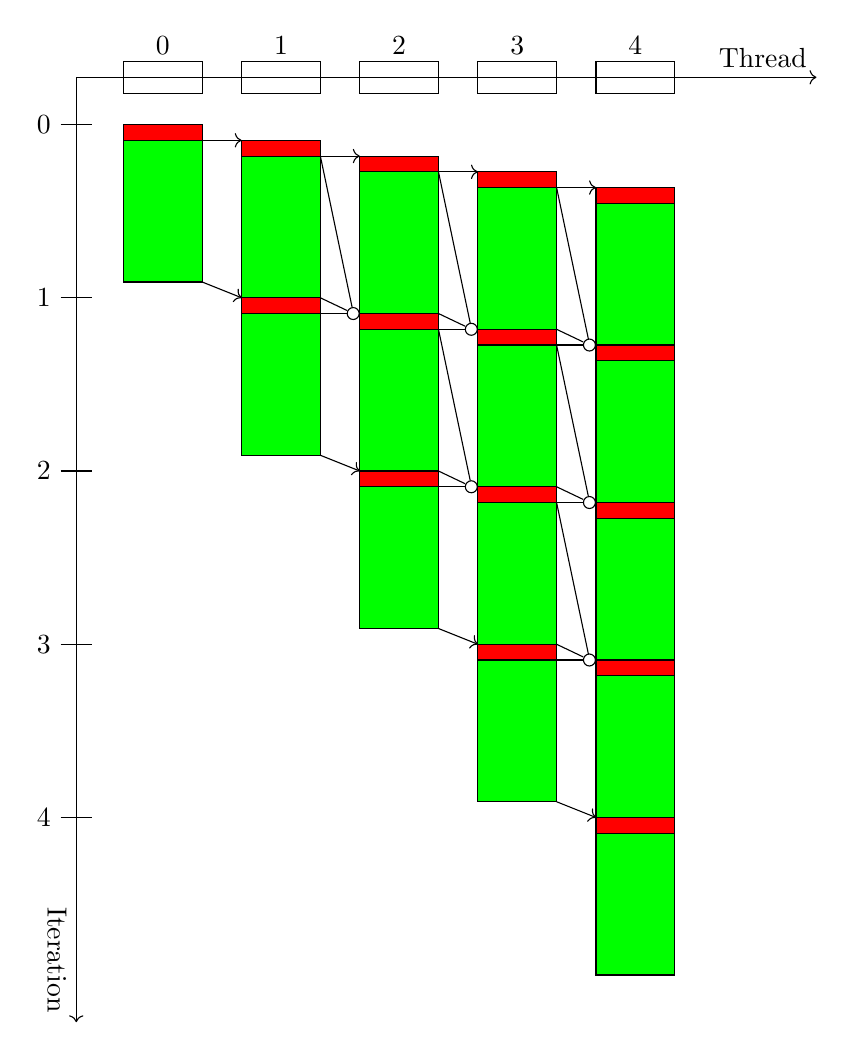
\begin{tikzpicture}[scale=2]
    \newcommand\Threads{4}
    \newcommand\Threadsmm{3}

    % Y-Axis
    \draw[->] (-.3,.3) -- (-.3,-1*\Threads-1.7) node[pos=1,below left, sloped] {Iteration};
    \foreach \x in {0,...,\Threads} {
        \draw (-.4, -1.1*\x) -- (-.2, -1.1*\x) node [pos=0, left] {\x};
    }

    % X-Axis
    \draw[->] (-.3,.3) -- (.75*\Threads+1.4,.3) node[pos=1,above left] {Thread};
    \foreach \x in {0,...,\Threads} {
        \draw(.75*\x, .2) rectangle (.5+0.75*\x, .4);
        \node at (0.75*\x+.25,.5) {\x};
        }


    % Computatations
    \foreach \y in {0,...,\Threads} {
        \foreach \x in {\y,...,\Threads} {
            \draw[fill=red] (.75*\x,-\y-.1-.1*\x) rectangle (.5+0.75*\x, -\y-.1*\x);
            \draw[fill=green] (.75*\x,-\y-1-.1*\x) rectangle (.5+0.75*\x, -\y-.1-.1*\x);
        }
    }

    % Communication
    % init
    \foreach \x in {0,...,\Threadsmm} {
        \draw[->] (.5+0.75*\x,-.1*\x-.1) -- (.75+0.75*\x,-.1*\x-.1);
    }
    % first of every iteration
    \foreach \x in {0,...,\Threadsmm} {
        \draw[->] (.5+0.75*\x,-1.1*\x-1) -- (.75+0.75*\x,-1.1*\x-1.1);
    }
    % merges
    \foreach \y in {1,...,\Threadsmm} {
        \foreach \x in {\y,...,\Threadsmm} {
        % previous coarse
        \draw[shorten >=0.08cm] (.5+0.75*\x,-\y-.1*\x+.9) -- (.71+0.75*\x,-\y-.1-.1*\x);
        % fine
        \draw[ shorten >=0.09cm] (.5+0.75*\x,-\y-.1*\x) -- (.71+0.75*\x,-\y-.1-.1*\x);
        % coarse
        \draw[-o, shorten >=0.0cm] (.5+0.75*\x,-\y-.1*\x-.1) -- (.75+0.75*\x,-\y-.1-.1*\x);
        }
    }



\end{tikzpicture}


\end{document}}}
    \caption{Utilization and communication of the threads}
    \label{fig:sequence}
\end{figure}
\begin{equation*}
y_{j+1}^{k+1} = \mathcal{G}\!\!\left(y_j^{k+1}, t_j, t_{j+1}\right) + \mathcal{F}\!\!\left(y_j^k, t_j, t_{j+1}\right) - \mathcal{G}\!\!\left(y_j^k, t_j, t_{j+1}\right)
\end{equation*}
\end{frame}

\subsection{Example}

\begin{frame}
\frametitle{Logistic equation}
\begin{equation*}
    y'(t) = k \cdot y(t) \cdot (L - y(t))
\end{equation*}
With \(y(0)= \frac{L}{2}\):
\begin{equation*}
    y(t) = \frac{L}{1+e^{-k L t}}
\end{equation*}
\end{frame}

\begin{frame}
    \begin{figure}[ht]
        \centering
        \scalebox{0.8}{%% Creator: Matplotlib, PGF backend
%%
%% To include the figure in your LaTeX document, write
%%   \input{<filename>.pgf}
%%
%% Make sure the required packages are loaded in your preamble
%%   \usepackage{pgf}
%%
%% Figures using additional raster images can only be included by \input if
%% they are in the same directory as the main LaTeX file. For loading figures
%% from other directories you can use the `import` package
%%   \usepackage{import}
%% and then include the figures with
%%   \import{<path to file>}{<filename>.pgf}
%%
%% Matplotlib used the following preamble
%%   \usepackage{fontspec}
%%   \setmainfont{Times New Roman}
%%   \setsansfont{Lucida Grande}
%%   \setmonofont{Andale Mono}
%%
\begingroup%
\makeatletter%
\begin{pgfpicture}%
\pgfpathrectangle{\pgfpointorigin}{\pgfqpoint{5.000000in}{3.000000in}}%
\pgfusepath{use as bounding box, clip}%
\begin{pgfscope}%
\pgfsetbuttcap%
\pgfsetmiterjoin%
\definecolor{currentfill}{rgb}{1.000000,1.000000,1.000000}%
\pgfsetfillcolor{currentfill}%
\pgfsetlinewidth{0.000000pt}%
\definecolor{currentstroke}{rgb}{1.000000,1.000000,1.000000}%
\pgfsetstrokecolor{currentstroke}%
\pgfsetdash{}{0pt}%
\pgfpathmoveto{\pgfqpoint{0.000000in}{0.000000in}}%
\pgfpathlineto{\pgfqpoint{5.000000in}{0.000000in}}%
\pgfpathlineto{\pgfqpoint{5.000000in}{3.000000in}}%
\pgfpathlineto{\pgfqpoint{0.000000in}{3.000000in}}%
\pgfpathclose%
\pgfusepath{fill}%
\end{pgfscope}%
\begin{pgfscope}%
\pgfsetbuttcap%
\pgfsetmiterjoin%
\definecolor{currentfill}{rgb}{1.000000,1.000000,1.000000}%
\pgfsetfillcolor{currentfill}%
\pgfsetlinewidth{0.000000pt}%
\definecolor{currentstroke}{rgb}{0.000000,0.000000,0.000000}%
\pgfsetstrokecolor{currentstroke}%
\pgfsetstrokeopacity{0.000000}%
\pgfsetdash{}{0pt}%
\pgfpathmoveto{\pgfqpoint{0.467954in}{0.402778in}}%
\pgfpathlineto{\pgfqpoint{4.951389in}{0.402778in}}%
\pgfpathlineto{\pgfqpoint{4.951389in}{2.951389in}}%
\pgfpathlineto{\pgfqpoint{0.467954in}{2.951389in}}%
\pgfpathclose%
\pgfusepath{fill}%
\end{pgfscope}%
\begin{pgfscope}%
\pgfsetbuttcap%
\pgfsetroundjoin%
\definecolor{currentfill}{rgb}{0.000000,0.000000,0.000000}%
\pgfsetfillcolor{currentfill}%
\pgfsetlinewidth{0.803000pt}%
\definecolor{currentstroke}{rgb}{0.000000,0.000000,0.000000}%
\pgfsetstrokecolor{currentstroke}%
\pgfsetdash{}{0pt}%
\pgfsys@defobject{currentmarker}{\pgfqpoint{0.000000in}{-0.048611in}}{\pgfqpoint{0.000000in}{0.000000in}}{%
\pgfpathmoveto{\pgfqpoint{0.000000in}{0.000000in}}%
\pgfpathlineto{\pgfqpoint{0.000000in}{-0.048611in}}%
\pgfusepath{stroke,fill}%
}%
\begin{pgfscope}%
\pgfsys@transformshift{0.671747in}{0.402778in}%
\pgfsys@useobject{currentmarker}{}%
\end{pgfscope}%
\end{pgfscope}%
\begin{pgfscope}%
\pgftext[x=0.671747in,y=0.305556in,,top]{\rmfamily\fontsize{10.000000}{12.000000}\selectfont \(\displaystyle -6\)}%
\end{pgfscope}%
\begin{pgfscope}%
\pgfsetbuttcap%
\pgfsetroundjoin%
\definecolor{currentfill}{rgb}{0.000000,0.000000,0.000000}%
\pgfsetfillcolor{currentfill}%
\pgfsetlinewidth{0.803000pt}%
\definecolor{currentstroke}{rgb}{0.000000,0.000000,0.000000}%
\pgfsetstrokecolor{currentstroke}%
\pgfsetdash{}{0pt}%
\pgfsys@defobject{currentmarker}{\pgfqpoint{0.000000in}{-0.048611in}}{\pgfqpoint{0.000000in}{0.000000in}}{%
\pgfpathmoveto{\pgfqpoint{0.000000in}{0.000000in}}%
\pgfpathlineto{\pgfqpoint{0.000000in}{-0.048611in}}%
\pgfusepath{stroke,fill}%
}%
\begin{pgfscope}%
\pgfsys@transformshift{1.351055in}{0.402778in}%
\pgfsys@useobject{currentmarker}{}%
\end{pgfscope}%
\end{pgfscope}%
\begin{pgfscope}%
\pgftext[x=1.351055in,y=0.305556in,,top]{\rmfamily\fontsize{10.000000}{12.000000}\selectfont \(\displaystyle -4\)}%
\end{pgfscope}%
\begin{pgfscope}%
\pgfsetbuttcap%
\pgfsetroundjoin%
\definecolor{currentfill}{rgb}{0.000000,0.000000,0.000000}%
\pgfsetfillcolor{currentfill}%
\pgfsetlinewidth{0.803000pt}%
\definecolor{currentstroke}{rgb}{0.000000,0.000000,0.000000}%
\pgfsetstrokecolor{currentstroke}%
\pgfsetdash{}{0pt}%
\pgfsys@defobject{currentmarker}{\pgfqpoint{0.000000in}{-0.048611in}}{\pgfqpoint{0.000000in}{0.000000in}}{%
\pgfpathmoveto{\pgfqpoint{0.000000in}{0.000000in}}%
\pgfpathlineto{\pgfqpoint{0.000000in}{-0.048611in}}%
\pgfusepath{stroke,fill}%
}%
\begin{pgfscope}%
\pgfsys@transformshift{2.030363in}{0.402778in}%
\pgfsys@useobject{currentmarker}{}%
\end{pgfscope}%
\end{pgfscope}%
\begin{pgfscope}%
\pgftext[x=2.030363in,y=0.305556in,,top]{\rmfamily\fontsize{10.000000}{12.000000}\selectfont \(\displaystyle -2\)}%
\end{pgfscope}%
\begin{pgfscope}%
\pgfsetbuttcap%
\pgfsetroundjoin%
\definecolor{currentfill}{rgb}{0.000000,0.000000,0.000000}%
\pgfsetfillcolor{currentfill}%
\pgfsetlinewidth{0.803000pt}%
\definecolor{currentstroke}{rgb}{0.000000,0.000000,0.000000}%
\pgfsetstrokecolor{currentstroke}%
\pgfsetdash{}{0pt}%
\pgfsys@defobject{currentmarker}{\pgfqpoint{0.000000in}{-0.048611in}}{\pgfqpoint{0.000000in}{0.000000in}}{%
\pgfpathmoveto{\pgfqpoint{0.000000in}{0.000000in}}%
\pgfpathlineto{\pgfqpoint{0.000000in}{-0.048611in}}%
\pgfusepath{stroke,fill}%
}%
\begin{pgfscope}%
\pgfsys@transformshift{2.709672in}{0.402778in}%
\pgfsys@useobject{currentmarker}{}%
\end{pgfscope}%
\end{pgfscope}%
\begin{pgfscope}%
\pgftext[x=2.709672in,y=0.305556in,,top]{\rmfamily\fontsize{10.000000}{12.000000}\selectfont \(\displaystyle 0\)}%
\end{pgfscope}%
\begin{pgfscope}%
\pgfsetbuttcap%
\pgfsetroundjoin%
\definecolor{currentfill}{rgb}{0.000000,0.000000,0.000000}%
\pgfsetfillcolor{currentfill}%
\pgfsetlinewidth{0.803000pt}%
\definecolor{currentstroke}{rgb}{0.000000,0.000000,0.000000}%
\pgfsetstrokecolor{currentstroke}%
\pgfsetdash{}{0pt}%
\pgfsys@defobject{currentmarker}{\pgfqpoint{0.000000in}{-0.048611in}}{\pgfqpoint{0.000000in}{0.000000in}}{%
\pgfpathmoveto{\pgfqpoint{0.000000in}{0.000000in}}%
\pgfpathlineto{\pgfqpoint{0.000000in}{-0.048611in}}%
\pgfusepath{stroke,fill}%
}%
\begin{pgfscope}%
\pgfsys@transformshift{3.388980in}{0.402778in}%
\pgfsys@useobject{currentmarker}{}%
\end{pgfscope}%
\end{pgfscope}%
\begin{pgfscope}%
\pgftext[x=3.388980in,y=0.305556in,,top]{\rmfamily\fontsize{10.000000}{12.000000}\selectfont \(\displaystyle 2\)}%
\end{pgfscope}%
\begin{pgfscope}%
\pgfsetbuttcap%
\pgfsetroundjoin%
\definecolor{currentfill}{rgb}{0.000000,0.000000,0.000000}%
\pgfsetfillcolor{currentfill}%
\pgfsetlinewidth{0.803000pt}%
\definecolor{currentstroke}{rgb}{0.000000,0.000000,0.000000}%
\pgfsetstrokecolor{currentstroke}%
\pgfsetdash{}{0pt}%
\pgfsys@defobject{currentmarker}{\pgfqpoint{0.000000in}{-0.048611in}}{\pgfqpoint{0.000000in}{0.000000in}}{%
\pgfpathmoveto{\pgfqpoint{0.000000in}{0.000000in}}%
\pgfpathlineto{\pgfqpoint{0.000000in}{-0.048611in}}%
\pgfusepath{stroke,fill}%
}%
\begin{pgfscope}%
\pgfsys@transformshift{4.068288in}{0.402778in}%
\pgfsys@useobject{currentmarker}{}%
\end{pgfscope}%
\end{pgfscope}%
\begin{pgfscope}%
\pgftext[x=4.068288in,y=0.305556in,,top]{\rmfamily\fontsize{10.000000}{12.000000}\selectfont \(\displaystyle 4\)}%
\end{pgfscope}%
\begin{pgfscope}%
\pgfsetbuttcap%
\pgfsetroundjoin%
\definecolor{currentfill}{rgb}{0.000000,0.000000,0.000000}%
\pgfsetfillcolor{currentfill}%
\pgfsetlinewidth{0.803000pt}%
\definecolor{currentstroke}{rgb}{0.000000,0.000000,0.000000}%
\pgfsetstrokecolor{currentstroke}%
\pgfsetdash{}{0pt}%
\pgfsys@defobject{currentmarker}{\pgfqpoint{0.000000in}{-0.048611in}}{\pgfqpoint{0.000000in}{0.000000in}}{%
\pgfpathmoveto{\pgfqpoint{0.000000in}{0.000000in}}%
\pgfpathlineto{\pgfqpoint{0.000000in}{-0.048611in}}%
\pgfusepath{stroke,fill}%
}%
\begin{pgfscope}%
\pgfsys@transformshift{4.747596in}{0.402778in}%
\pgfsys@useobject{currentmarker}{}%
\end{pgfscope}%
\end{pgfscope}%
\begin{pgfscope}%
\pgftext[x=4.747596in,y=0.305556in,,top]{\rmfamily\fontsize{10.000000}{12.000000}\selectfont \(\displaystyle 6\)}%
\end{pgfscope}%
\begin{pgfscope}%
\pgftext[x=2.709672in,y=0.123861in,,top]{\rmfamily\fontsize{10.000000}{12.000000}\selectfont t}%
\end{pgfscope}%
\begin{pgfscope}%
\pgfsetbuttcap%
\pgfsetroundjoin%
\definecolor{currentfill}{rgb}{0.000000,0.000000,0.000000}%
\pgfsetfillcolor{currentfill}%
\pgfsetlinewidth{0.803000pt}%
\definecolor{currentstroke}{rgb}{0.000000,0.000000,0.000000}%
\pgfsetstrokecolor{currentstroke}%
\pgfsetdash{}{0pt}%
\pgfsys@defobject{currentmarker}{\pgfqpoint{-0.048611in}{0.000000in}}{\pgfqpoint{0.000000in}{0.000000in}}{%
\pgfpathmoveto{\pgfqpoint{0.000000in}{0.000000in}}%
\pgfpathlineto{\pgfqpoint{-0.048611in}{0.000000in}}%
\pgfusepath{stroke,fill}%
}%
\begin{pgfscope}%
\pgfsys@transformshift{0.467954in}{0.512870in}%
\pgfsys@useobject{currentmarker}{}%
\end{pgfscope}%
\end{pgfscope}%
\begin{pgfscope}%
\pgftext[x=0.193262in,y=0.464653in,left,base]{\rmfamily\fontsize{10.000000}{12.000000}\selectfont \(\displaystyle 0.0\)}%
\end{pgfscope}%
\begin{pgfscope}%
\pgfsetbuttcap%
\pgfsetroundjoin%
\definecolor{currentfill}{rgb}{0.000000,0.000000,0.000000}%
\pgfsetfillcolor{currentfill}%
\pgfsetlinewidth{0.803000pt}%
\definecolor{currentstroke}{rgb}{0.000000,0.000000,0.000000}%
\pgfsetstrokecolor{currentstroke}%
\pgfsetdash{}{0pt}%
\pgfsys@defobject{currentmarker}{\pgfqpoint{-0.048611in}{0.000000in}}{\pgfqpoint{0.000000in}{0.000000in}}{%
\pgfpathmoveto{\pgfqpoint{0.000000in}{0.000000in}}%
\pgfpathlineto{\pgfqpoint{-0.048611in}{0.000000in}}%
\pgfusepath{stroke,fill}%
}%
\begin{pgfscope}%
\pgfsys@transformshift{0.467954in}{0.978232in}%
\pgfsys@useobject{currentmarker}{}%
\end{pgfscope}%
\end{pgfscope}%
\begin{pgfscope}%
\pgftext[x=0.193262in,y=0.930014in,left,base]{\rmfamily\fontsize{10.000000}{12.000000}\selectfont \(\displaystyle 0.2\)}%
\end{pgfscope}%
\begin{pgfscope}%
\pgfsetbuttcap%
\pgfsetroundjoin%
\definecolor{currentfill}{rgb}{0.000000,0.000000,0.000000}%
\pgfsetfillcolor{currentfill}%
\pgfsetlinewidth{0.803000pt}%
\definecolor{currentstroke}{rgb}{0.000000,0.000000,0.000000}%
\pgfsetstrokecolor{currentstroke}%
\pgfsetdash{}{0pt}%
\pgfsys@defobject{currentmarker}{\pgfqpoint{-0.048611in}{0.000000in}}{\pgfqpoint{0.000000in}{0.000000in}}{%
\pgfpathmoveto{\pgfqpoint{0.000000in}{0.000000in}}%
\pgfpathlineto{\pgfqpoint{-0.048611in}{0.000000in}}%
\pgfusepath{stroke,fill}%
}%
\begin{pgfscope}%
\pgfsys@transformshift{0.467954in}{1.443594in}%
\pgfsys@useobject{currentmarker}{}%
\end{pgfscope}%
\end{pgfscope}%
\begin{pgfscope}%
\pgftext[x=0.193262in,y=1.395376in,left,base]{\rmfamily\fontsize{10.000000}{12.000000}\selectfont \(\displaystyle 0.4\)}%
\end{pgfscope}%
\begin{pgfscope}%
\pgfsetbuttcap%
\pgfsetroundjoin%
\definecolor{currentfill}{rgb}{0.000000,0.000000,0.000000}%
\pgfsetfillcolor{currentfill}%
\pgfsetlinewidth{0.803000pt}%
\definecolor{currentstroke}{rgb}{0.000000,0.000000,0.000000}%
\pgfsetstrokecolor{currentstroke}%
\pgfsetdash{}{0pt}%
\pgfsys@defobject{currentmarker}{\pgfqpoint{-0.048611in}{0.000000in}}{\pgfqpoint{0.000000in}{0.000000in}}{%
\pgfpathmoveto{\pgfqpoint{0.000000in}{0.000000in}}%
\pgfpathlineto{\pgfqpoint{-0.048611in}{0.000000in}}%
\pgfusepath{stroke,fill}%
}%
\begin{pgfscope}%
\pgfsys@transformshift{0.467954in}{1.908956in}%
\pgfsys@useobject{currentmarker}{}%
\end{pgfscope}%
\end{pgfscope}%
\begin{pgfscope}%
\pgftext[x=0.193262in,y=1.860738in,left,base]{\rmfamily\fontsize{10.000000}{12.000000}\selectfont \(\displaystyle 0.6\)}%
\end{pgfscope}%
\begin{pgfscope}%
\pgfsetbuttcap%
\pgfsetroundjoin%
\definecolor{currentfill}{rgb}{0.000000,0.000000,0.000000}%
\pgfsetfillcolor{currentfill}%
\pgfsetlinewidth{0.803000pt}%
\definecolor{currentstroke}{rgb}{0.000000,0.000000,0.000000}%
\pgfsetstrokecolor{currentstroke}%
\pgfsetdash{}{0pt}%
\pgfsys@defobject{currentmarker}{\pgfqpoint{-0.048611in}{0.000000in}}{\pgfqpoint{0.000000in}{0.000000in}}{%
\pgfpathmoveto{\pgfqpoint{0.000000in}{0.000000in}}%
\pgfpathlineto{\pgfqpoint{-0.048611in}{0.000000in}}%
\pgfusepath{stroke,fill}%
}%
\begin{pgfscope}%
\pgfsys@transformshift{0.467954in}{2.374317in}%
\pgfsys@useobject{currentmarker}{}%
\end{pgfscope}%
\end{pgfscope}%
\begin{pgfscope}%
\pgftext[x=0.193262in,y=2.326100in,left,base]{\rmfamily\fontsize{10.000000}{12.000000}\selectfont \(\displaystyle 0.8\)}%
\end{pgfscope}%
\begin{pgfscope}%
\pgfsetbuttcap%
\pgfsetroundjoin%
\definecolor{currentfill}{rgb}{0.000000,0.000000,0.000000}%
\pgfsetfillcolor{currentfill}%
\pgfsetlinewidth{0.803000pt}%
\definecolor{currentstroke}{rgb}{0.000000,0.000000,0.000000}%
\pgfsetstrokecolor{currentstroke}%
\pgfsetdash{}{0pt}%
\pgfsys@defobject{currentmarker}{\pgfqpoint{-0.048611in}{0.000000in}}{\pgfqpoint{0.000000in}{0.000000in}}{%
\pgfpathmoveto{\pgfqpoint{0.000000in}{0.000000in}}%
\pgfpathlineto{\pgfqpoint{-0.048611in}{0.000000in}}%
\pgfusepath{stroke,fill}%
}%
\begin{pgfscope}%
\pgfsys@transformshift{0.467954in}{2.839679in}%
\pgfsys@useobject{currentmarker}{}%
\end{pgfscope}%
\end{pgfscope}%
\begin{pgfscope}%
\pgftext[x=0.193262in,y=2.791461in,left,base]{\rmfamily\fontsize{10.000000}{12.000000}\selectfont \(\displaystyle 1.0\)}%
\end{pgfscope}%
\begin{pgfscope}%
\pgftext[x=0.137707in,y=1.677083in,,bottom,rotate=90.000000]{\rmfamily\fontsize{10.000000}{12.000000}\selectfont y(t)}%
\end{pgfscope}%
\begin{pgfscope}%
\pgfpathrectangle{\pgfqpoint{0.467954in}{0.402778in}}{\pgfqpoint{4.483434in}{2.548611in}}%
\pgfusepath{clip}%
\pgfsetrectcap%
\pgfsetroundjoin%
\pgfsetlinewidth{1.505625pt}%
\definecolor{currentstroke}{rgb}{0.121569,0.466667,0.705882}%
\pgfsetstrokecolor{currentstroke}%
\pgfsetdash{}{0pt}%
\pgfpathmoveto{\pgfqpoint{0.671747in}{0.518624in}}%
\pgfpathlineto{\pgfqpoint{0.894583in}{0.523933in}}%
\pgfpathlineto{\pgfqpoint{1.011318in}{0.528440in}}%
\pgfpathlineto{\pgfqpoint{1.012873in}{0.532894in}}%
\pgfpathlineto{\pgfqpoint{1.139994in}{0.541870in}}%
\pgfpathlineto{\pgfqpoint{1.247463in}{0.552479in}}%
\pgfpathlineto{\pgfqpoint{1.340939in}{0.564748in}}%
\pgfpathlineto{\pgfqpoint{1.350952in}{0.566265in}}%
\pgfpathlineto{\pgfqpoint{1.352506in}{0.580630in}}%
\pgfpathlineto{\pgfqpoint{1.426578in}{0.596549in}}%
\pgfpathlineto{\pgfqpoint{1.494492in}{0.614263in}}%
\pgfpathlineto{\pgfqpoint{1.557555in}{0.633874in}}%
\pgfpathlineto{\pgfqpoint{1.616638in}{0.655455in}}%
\pgfpathlineto{\pgfqpoint{1.672549in}{0.679145in}}%
\pgfpathlineto{\pgfqpoint{1.690585in}{0.687533in}}%
\pgfpathlineto{\pgfqpoint{1.692140in}{0.726096in}}%
\pgfpathlineto{\pgfqpoint{1.742267in}{0.756455in}}%
\pgfpathlineto{\pgfqpoint{1.791150in}{0.789674in}}%
\pgfpathlineto{\pgfqpoint{1.839163in}{0.826046in}}%
\pgfpathlineto{\pgfqpoint{1.886678in}{0.865935in}}%
\pgfpathlineto{\pgfqpoint{1.934069in}{0.909781in}}%
\pgfpathlineto{\pgfqpoint{1.981646in}{0.958043in}}%
\pgfpathlineto{\pgfqpoint{2.029845in}{1.011376in}}%
\pgfpathlineto{\pgfqpoint{2.030218in}{1.011806in}}%
\pgfpathlineto{\pgfqpoint{2.031773in}{1.074884in}}%
\pgfpathlineto{\pgfqpoint{2.083020in}{1.141677in}}%
\pgfpathlineto{\pgfqpoint{2.136941in}{1.217118in}}%
\pgfpathlineto{\pgfqpoint{2.195028in}{1.303820in}}%
\pgfpathlineto{\pgfqpoint{2.259957in}{1.406451in}}%
\pgfpathlineto{\pgfqpoint{2.338880in}{1.537282in}}%
\pgfpathlineto{\pgfqpoint{2.369852in}{1.589818in}}%
\pgfpathlineto{\pgfqpoint{2.371407in}{1.624306in}}%
\pgfpathlineto{\pgfqpoint{2.545546in}{1.918895in}}%
\pgfpathlineto{\pgfqpoint{2.617440in}{2.033707in}}%
\pgfpathlineto{\pgfqpoint{2.679135in}{2.126549in}}%
\pgfpathlineto{\pgfqpoint{2.709485in}{2.169961in}}%
\pgfpathlineto{\pgfqpoint{2.709547in}{2.155912in}}%
\pgfpathlineto{\pgfqpoint{2.711040in}{2.158032in}}%
\pgfpathlineto{\pgfqpoint{2.765894in}{2.233191in}}%
\pgfpathlineto{\pgfqpoint{2.817949in}{2.299357in}}%
\pgfpathlineto{\pgfqpoint{2.868138in}{2.358221in}}%
\pgfpathlineto{\pgfqpoint{2.917146in}{2.410992in}}%
\pgfpathlineto{\pgfqpoint{2.965470in}{2.458530in}}%
\pgfpathlineto{\pgfqpoint{3.013544in}{2.501523in}}%
\pgfpathlineto{\pgfqpoint{3.049118in}{2.530684in}}%
\pgfpathlineto{\pgfqpoint{3.049181in}{2.508546in}}%
\pgfpathlineto{\pgfqpoint{3.050673in}{2.509792in}}%
\pgfpathlineto{\pgfqpoint{3.098935in}{2.548011in}}%
\pgfpathlineto{\pgfqpoint{3.147756in}{2.582749in}}%
\pgfpathlineto{\pgfqpoint{3.197510in}{2.614368in}}%
\pgfpathlineto{\pgfqpoint{3.248570in}{2.643160in}}%
\pgfpathlineto{\pgfqpoint{3.301371in}{2.669383in}}%
\pgfpathlineto{\pgfqpoint{3.356412in}{2.693256in}}%
\pgfpathlineto{\pgfqpoint{3.388752in}{2.705790in}}%
\pgfpathlineto{\pgfqpoint{3.388814in}{2.691892in}}%
\pgfpathlineto{\pgfqpoint{3.390307in}{2.692499in}}%
\pgfpathlineto{\pgfqpoint{3.448021in}{2.714259in}}%
\pgfpathlineto{\pgfqpoint{3.509094in}{2.733962in}}%
\pgfpathlineto{\pgfqpoint{3.574397in}{2.751754in}}%
\pgfpathlineto{\pgfqpoint{3.644923in}{2.767730in}}%
\pgfpathlineto{\pgfqpoint{3.721979in}{2.781972in}}%
\pgfpathlineto{\pgfqpoint{3.728447in}{2.783034in}}%
\pgfpathlineto{\pgfqpoint{3.728510in}{2.776244in}}%
\pgfpathlineto{\pgfqpoint{3.730002in}{2.776514in}}%
\pgfpathlineto{\pgfqpoint{3.811723in}{2.789732in}}%
\pgfpathlineto{\pgfqpoint{3.903022in}{2.801310in}}%
\pgfpathlineto{\pgfqpoint{4.006821in}{2.811290in}}%
\pgfpathlineto{\pgfqpoint{4.068143in}{2.815932in}}%
\pgfpathlineto{\pgfqpoint{4.068205in}{2.812914in}}%
\pgfpathlineto{\pgfqpoint{4.069698in}{2.813030in}}%
\pgfpathlineto{\pgfqpoint{4.194394in}{2.821153in}}%
\pgfpathlineto{\pgfqpoint{4.344900in}{2.827751in}}%
\pgfpathlineto{\pgfqpoint{4.427927in}{2.829108in}}%
\pgfpathlineto{\pgfqpoint{4.630861in}{2.833851in}}%
\pgfpathlineto{\pgfqpoint{4.747596in}{2.835543in}}%
\pgfpathlineto{\pgfqpoint{4.747596in}{2.835543in}}%
\pgfusepath{stroke}%
\end{pgfscope}%
\begin{pgfscope}%
\pgfpathrectangle{\pgfqpoint{0.467954in}{0.402778in}}{\pgfqpoint{4.483434in}{2.548611in}}%
\pgfusepath{clip}%
\pgfsetrectcap%
\pgfsetroundjoin%
\pgfsetlinewidth{1.505625pt}%
\definecolor{currentstroke}{rgb}{1.000000,0.498039,0.054902}%
\pgfsetstrokecolor{currentstroke}%
\pgfsetdash{}{0pt}%
\pgfpathmoveto{\pgfqpoint{0.671747in}{0.518624in}}%
\pgfpathlineto{\pgfqpoint{0.894583in}{0.523933in}}%
\pgfpathlineto{\pgfqpoint{1.060886in}{0.530867in}}%
\pgfpathlineto{\pgfqpoint{1.194289in}{0.539426in}}%
\pgfpathlineto{\pgfqpoint{1.306111in}{0.549616in}}%
\pgfpathlineto{\pgfqpoint{1.350952in}{0.554708in}}%
\pgfpathlineto{\pgfqpoint{1.351014in}{0.551882in}}%
\pgfpathlineto{\pgfqpoint{1.352506in}{0.552051in}}%
\pgfpathlineto{\pgfqpoint{1.446417in}{0.564254in}}%
\pgfpathlineto{\pgfqpoint{1.529755in}{0.578142in}}%
\pgfpathlineto{\pgfqpoint{1.605008in}{0.593768in}}%
\pgfpathlineto{\pgfqpoint{1.673855in}{0.611178in}}%
\pgfpathlineto{\pgfqpoint{1.690585in}{0.615921in}}%
\pgfpathlineto{\pgfqpoint{1.690647in}{0.603281in}}%
\pgfpathlineto{\pgfqpoint{1.692140in}{0.603664in}}%
\pgfpathlineto{\pgfqpoint{1.757939in}{0.622160in}}%
\pgfpathlineto{\pgfqpoint{1.819261in}{0.642580in}}%
\pgfpathlineto{\pgfqpoint{1.876976in}{0.665032in}}%
\pgfpathlineto{\pgfqpoint{1.931768in}{0.689645in}}%
\pgfpathlineto{\pgfqpoint{1.984258in}{0.716602in}}%
\pgfpathlineto{\pgfqpoint{2.030218in}{0.743200in}}%
\pgfpathlineto{\pgfqpoint{2.030280in}{0.727386in}}%
\pgfpathlineto{\pgfqpoint{2.031773in}{0.728243in}}%
\pgfpathlineto{\pgfqpoint{2.081838in}{0.758832in}}%
\pgfpathlineto{\pgfqpoint{2.130659in}{0.792288in}}%
\pgfpathlineto{\pgfqpoint{2.178610in}{0.828900in}}%
\pgfpathlineto{\pgfqpoint{2.226125in}{0.869087in}}%
\pgfpathlineto{\pgfqpoint{2.273515in}{0.913246in}}%
\pgfpathlineto{\pgfqpoint{2.321155in}{0.961897in}}%
\pgfpathlineto{\pgfqpoint{2.369416in}{1.015641in}}%
\pgfpathlineto{\pgfqpoint{2.369852in}{1.016146in}}%
\pgfpathlineto{\pgfqpoint{2.371407in}{1.047363in}}%
\pgfpathlineto{\pgfqpoint{2.421720in}{1.110774in}}%
\pgfpathlineto{\pgfqpoint{2.474273in}{1.182050in}}%
\pgfpathlineto{\pgfqpoint{2.530246in}{1.263272in}}%
\pgfpathlineto{\pgfqpoint{2.591630in}{1.357931in}}%
\pgfpathlineto{\pgfqpoint{2.662778in}{1.473549in}}%
\pgfpathlineto{\pgfqpoint{2.709485in}{1.551927in}}%
\pgfpathlineto{\pgfqpoint{2.711040in}{1.603719in}}%
\pgfpathlineto{\pgfqpoint{2.905329in}{1.932122in}}%
\pgfpathlineto{\pgfqpoint{2.975731in}{2.043916in}}%
\pgfpathlineto{\pgfqpoint{3.036742in}{2.135137in}}%
\pgfpathlineto{\pgfqpoint{3.049118in}{2.152906in}}%
\pgfpathlineto{\pgfqpoint{3.050735in}{2.164216in}}%
\pgfpathlineto{\pgfqpoint{3.105341in}{2.238616in}}%
\pgfpathlineto{\pgfqpoint{3.157209in}{2.304147in}}%
\pgfpathlineto{\pgfqpoint{3.207274in}{2.362490in}}%
\pgfpathlineto{\pgfqpoint{3.256220in}{2.414837in}}%
\pgfpathlineto{\pgfqpoint{3.304481in}{2.461976in}}%
\pgfpathlineto{\pgfqpoint{3.352556in}{2.504648in}}%
\pgfpathlineto{\pgfqpoint{3.388752in}{2.534066in}}%
\pgfpathlineto{\pgfqpoint{3.388814in}{2.525917in}}%
\pgfpathlineto{\pgfqpoint{3.390307in}{2.527108in}}%
\pgfpathlineto{\pgfqpoint{3.438755in}{2.563731in}}%
\pgfpathlineto{\pgfqpoint{3.487949in}{2.597059in}}%
\pgfpathlineto{\pgfqpoint{3.538201in}{2.627381in}}%
\pgfpathlineto{\pgfqpoint{3.589945in}{2.654999in}}%
\pgfpathlineto{\pgfqpoint{3.643679in}{2.680170in}}%
\pgfpathlineto{\pgfqpoint{3.699839in}{2.703051in}}%
\pgfpathlineto{\pgfqpoint{3.728447in}{2.713490in}}%
\pgfpathlineto{\pgfqpoint{3.728510in}{2.706993in}}%
\pgfpathlineto{\pgfqpoint{3.730002in}{2.707542in}}%
\pgfpathlineto{\pgfqpoint{3.789956in}{2.727896in}}%
\pgfpathlineto{\pgfqpoint{3.853828in}{2.746289in}}%
\pgfpathlineto{\pgfqpoint{3.922550in}{2.762831in}}%
\pgfpathlineto{\pgfqpoint{3.997368in}{2.777619in}}%
\pgfpathlineto{\pgfqpoint{4.068143in}{2.789038in}}%
\pgfpathlineto{\pgfqpoint{4.068205in}{2.785924in}}%
\pgfpathlineto{\pgfqpoint{4.069698in}{2.786154in}}%
\pgfpathlineto{\pgfqpoint{4.158011in}{2.798191in}}%
\pgfpathlineto{\pgfqpoint{4.257892in}{2.808620in}}%
\pgfpathlineto{\pgfqpoint{4.373260in}{2.817479in}}%
\pgfpathlineto{\pgfqpoint{4.438873in}{2.820180in}}%
\pgfpathlineto{\pgfqpoint{4.585398in}{2.826975in}}%
\pgfpathlineto{\pgfqpoint{4.747596in}{2.831782in}}%
\pgfpathlineto{\pgfqpoint{4.747596in}{2.831782in}}%
\pgfusepath{stroke}%
\end{pgfscope}%
\begin{pgfscope}%
\pgfpathrectangle{\pgfqpoint{0.467954in}{0.402778in}}{\pgfqpoint{4.483434in}{2.548611in}}%
\pgfusepath{clip}%
\pgfsetrectcap%
\pgfsetroundjoin%
\pgfsetlinewidth{1.505625pt}%
\definecolor{currentstroke}{rgb}{0.172549,0.627451,0.172549}%
\pgfsetstrokecolor{currentstroke}%
\pgfsetdash{}{0pt}%
\pgfpathmoveto{\pgfqpoint{0.671747in}{0.518624in}}%
\pgfpathlineto{\pgfqpoint{0.894583in}{0.523933in}}%
\pgfpathlineto{\pgfqpoint{1.060886in}{0.530867in}}%
\pgfpathlineto{\pgfqpoint{1.194289in}{0.539426in}}%
\pgfpathlineto{\pgfqpoint{1.306111in}{0.549616in}}%
\pgfpathlineto{\pgfqpoint{1.402758in}{0.561458in}}%
\pgfpathlineto{\pgfqpoint{1.488148in}{0.574975in}}%
\pgfpathlineto{\pgfqpoint{1.565018in}{0.590224in}}%
\pgfpathlineto{\pgfqpoint{1.635171in}{0.607251in}}%
\pgfpathlineto{\pgfqpoint{1.690585in}{0.623183in}}%
\pgfpathlineto{\pgfqpoint{1.692202in}{0.625135in}}%
\pgfpathlineto{\pgfqpoint{1.752902in}{0.645847in}}%
\pgfpathlineto{\pgfqpoint{1.810119in}{0.668613in}}%
\pgfpathlineto{\pgfqpoint{1.864537in}{0.693574in}}%
\pgfpathlineto{\pgfqpoint{1.916717in}{0.720897in}}%
\pgfpathlineto{\pgfqpoint{1.967155in}{0.750795in}}%
\pgfpathlineto{\pgfqpoint{2.016225in}{0.783475in}}%
\pgfpathlineto{\pgfqpoint{2.030218in}{0.793483in}}%
\pgfpathlineto{\pgfqpoint{2.031835in}{0.800068in}}%
\pgfpathlineto{\pgfqpoint{2.079661in}{0.837436in}}%
\pgfpathlineto{\pgfqpoint{2.127114in}{0.878455in}}%
\pgfpathlineto{\pgfqpoint{2.174505in}{0.923533in}}%
\pgfpathlineto{\pgfqpoint{2.222207in}{0.973203in}}%
\pgfpathlineto{\pgfqpoint{2.270717in}{1.028223in}}%
\pgfpathlineto{\pgfqpoint{2.320471in}{1.089380in}}%
\pgfpathlineto{\pgfqpoint{2.388012in}{1.178118in}}%
\pgfpathlineto{\pgfqpoint{2.443799in}{1.258799in}}%
\pgfpathlineto{\pgfqpoint{2.504809in}{1.352604in}}%
\pgfpathlineto{\pgfqpoint{2.575274in}{1.466830in}}%
\pgfpathlineto{\pgfqpoint{2.670179in}{1.627090in}}%
\pgfpathlineto{\pgfqpoint{2.709485in}{1.694375in}}%
\pgfpathlineto{\pgfqpoint{2.709547in}{1.682284in}}%
\pgfpathlineto{\pgfqpoint{2.711040in}{1.684841in}}%
\pgfpathlineto{\pgfqpoint{2.842142in}{1.906300in}}%
\pgfpathlineto{\pgfqpoint{2.915467in}{2.024001in}}%
\pgfpathlineto{\pgfqpoint{2.977846in}{2.118433in}}%
\pgfpathlineto{\pgfqpoint{3.034565in}{2.198804in}}%
\pgfpathlineto{\pgfqpoint{3.049118in}{2.218508in}}%
\pgfpathlineto{\pgfqpoint{3.049181in}{2.215073in}}%
\pgfpathlineto{\pgfqpoint{3.050673in}{2.217079in}}%
\pgfpathlineto{\pgfqpoint{3.103288in}{2.285131in}}%
\pgfpathlineto{\pgfqpoint{3.153851in}{2.345544in}}%
\pgfpathlineto{\pgfqpoint{3.203045in}{2.399569in}}%
\pgfpathlineto{\pgfqpoint{3.251493in}{2.448232in}}%
\pgfpathlineto{\pgfqpoint{3.299568in}{2.492179in}}%
\pgfpathlineto{\pgfqpoint{3.347705in}{2.532026in}}%
\pgfpathlineto{\pgfqpoint{3.404300in}{2.574546in}}%
\pgfpathlineto{\pgfqpoint{3.453805in}{2.606908in}}%
\pgfpathlineto{\pgfqpoint{3.504492in}{2.636358in}}%
\pgfpathlineto{\pgfqpoint{3.556796in}{2.663175in}}%
\pgfpathlineto{\pgfqpoint{3.611215in}{2.687597in}}%
\pgfpathlineto{\pgfqpoint{3.668245in}{2.709792in}}%
\pgfpathlineto{\pgfqpoint{3.749469in}{2.737480in}}%
\pgfpathlineto{\pgfqpoint{3.815704in}{2.754927in}}%
\pgfpathlineto{\pgfqpoint{3.887349in}{2.770566in}}%
\pgfpathlineto{\pgfqpoint{3.965774in}{2.784478in}}%
\pgfpathlineto{\pgfqpoint{4.052844in}{2.796730in}}%
\pgfpathlineto{\pgfqpoint{4.174741in}{2.810305in}}%
\pgfpathlineto{\pgfqpoint{4.293404in}{2.818889in}}%
\pgfpathlineto{\pgfqpoint{4.460454in}{2.827477in}}%
\pgfpathlineto{\pgfqpoint{4.648275in}{2.832644in}}%
\pgfpathlineto{\pgfqpoint{4.747596in}{2.834424in}}%
\pgfpathlineto{\pgfqpoint{4.747596in}{2.834424in}}%
\pgfusepath{stroke}%
\end{pgfscope}%
\begin{pgfscope}%
\pgfpathrectangle{\pgfqpoint{0.467954in}{0.402778in}}{\pgfqpoint{4.483434in}{2.548611in}}%
\pgfusepath{clip}%
\pgfsetrectcap%
\pgfsetroundjoin%
\pgfsetlinewidth{1.505625pt}%
\definecolor{currentstroke}{rgb}{0.839216,0.152941,0.156863}%
\pgfsetstrokecolor{currentstroke}%
\pgfsetdash{}{0pt}%
\pgfpathmoveto{\pgfqpoint{0.671747in}{0.518624in}}%
\pgfpathlineto{\pgfqpoint{0.894583in}{0.523933in}}%
\pgfpathlineto{\pgfqpoint{1.060886in}{0.530867in}}%
\pgfpathlineto{\pgfqpoint{1.194289in}{0.539426in}}%
\pgfpathlineto{\pgfqpoint{1.306111in}{0.549616in}}%
\pgfpathlineto{\pgfqpoint{1.402758in}{0.561458in}}%
\pgfpathlineto{\pgfqpoint{1.488148in}{0.574975in}}%
\pgfpathlineto{\pgfqpoint{1.565018in}{0.590224in}}%
\pgfpathlineto{\pgfqpoint{1.635171in}{0.607251in}}%
\pgfpathlineto{\pgfqpoint{1.699976in}{0.626125in}}%
\pgfpathlineto{\pgfqpoint{1.760489in}{0.646939in}}%
\pgfpathlineto{\pgfqpoint{1.817582in}{0.669824in}}%
\pgfpathlineto{\pgfqpoint{1.871876in}{0.694902in}}%
\pgfpathlineto{\pgfqpoint{1.923931in}{0.722337in}}%
\pgfpathlineto{\pgfqpoint{1.974307in}{0.752379in}}%
\pgfpathlineto{\pgfqpoint{2.023377in}{0.785247in}}%
\pgfpathlineto{\pgfqpoint{2.075743in}{0.824216in}}%
\pgfpathlineto{\pgfqpoint{2.123258in}{0.863912in}}%
\pgfpathlineto{\pgfqpoint{2.170649in}{0.907557in}}%
\pgfpathlineto{\pgfqpoint{2.218226in}{0.955610in}}%
\pgfpathlineto{\pgfqpoint{2.266426in}{1.008729in}}%
\pgfpathlineto{\pgfqpoint{2.315682in}{1.067662in}}%
\pgfpathlineto{\pgfqpoint{2.366680in}{1.133565in}}%
\pgfpathlineto{\pgfqpoint{2.414755in}{1.200561in}}%
\pgfpathlineto{\pgfqpoint{2.471785in}{1.284590in}}%
\pgfpathlineto{\pgfqpoint{2.534973in}{1.383349in}}%
\pgfpathlineto{\pgfqpoint{2.609853in}{1.506378in}}%
\pgfpathlineto{\pgfqpoint{2.709485in}{1.675788in}}%
\pgfpathlineto{\pgfqpoint{2.711164in}{1.680286in}}%
\pgfpathlineto{\pgfqpoint{2.844816in}{1.906120in}}%
\pgfpathlineto{\pgfqpoint{2.918203in}{2.023927in}}%
\pgfpathlineto{\pgfqpoint{2.980582in}{2.118363in}}%
\pgfpathlineto{\pgfqpoint{3.037302in}{2.198739in}}%
\pgfpathlineto{\pgfqpoint{3.092280in}{2.271291in}}%
\pgfpathlineto{\pgfqpoint{3.143216in}{2.333216in}}%
\pgfpathlineto{\pgfqpoint{3.192659in}{2.388523in}}%
\pgfpathlineto{\pgfqpoint{3.241231in}{2.438269in}}%
\pgfpathlineto{\pgfqpoint{3.289368in}{2.483184in}}%
\pgfpathlineto{\pgfqpoint{3.337443in}{2.523848in}}%
\pgfpathlineto{\pgfqpoint{3.385829in}{2.560755in}}%
\pgfpathlineto{\pgfqpoint{3.434899in}{2.594319in}}%
\pgfpathlineto{\pgfqpoint{3.485088in}{2.624912in}}%
\pgfpathlineto{\pgfqpoint{3.536708in}{2.652760in}}%
\pgfpathlineto{\pgfqpoint{3.590256in}{2.678131in}}%
\pgfpathlineto{\pgfqpoint{3.646167in}{2.701191in}}%
\pgfpathlineto{\pgfqpoint{3.705063in}{2.722124in}}%
\pgfpathlineto{\pgfqpoint{3.767193in}{2.740917in}}%
\pgfpathlineto{\pgfqpoint{3.834361in}{2.758016in}}%
\pgfpathlineto{\pgfqpoint{3.907189in}{2.773326in}}%
\pgfpathlineto{\pgfqpoint{3.987106in}{2.786922in}}%
\pgfpathlineto{\pgfqpoint{4.073803in}{2.798522in}}%
\pgfpathlineto{\pgfqpoint{4.174119in}{2.808908in}}%
\pgfpathlineto{\pgfqpoint{4.290046in}{2.817722in}}%
\pgfpathlineto{\pgfqpoint{4.423822in}{2.824742in}}%
\pgfpathlineto{\pgfqpoint{4.592364in}{2.830562in}}%
\pgfpathlineto{\pgfqpoint{4.747596in}{2.833898in}}%
\pgfpathlineto{\pgfqpoint{4.747596in}{2.833898in}}%
\pgfusepath{stroke}%
\end{pgfscope}%
\begin{pgfscope}%
\pgfsetrectcap%
\pgfsetmiterjoin%
\pgfsetlinewidth{0.803000pt}%
\definecolor{currentstroke}{rgb}{0.000000,0.000000,0.000000}%
\pgfsetstrokecolor{currentstroke}%
\pgfsetdash{}{0pt}%
\pgfpathmoveto{\pgfqpoint{0.467954in}{0.402778in}}%
\pgfpathlineto{\pgfqpoint{0.467954in}{2.951389in}}%
\pgfusepath{stroke}%
\end{pgfscope}%
\begin{pgfscope}%
\pgfsetrectcap%
\pgfsetmiterjoin%
\pgfsetlinewidth{0.803000pt}%
\definecolor{currentstroke}{rgb}{0.000000,0.000000,0.000000}%
\pgfsetstrokecolor{currentstroke}%
\pgfsetdash{}{0pt}%
\pgfpathmoveto{\pgfqpoint{4.951389in}{0.402778in}}%
\pgfpathlineto{\pgfqpoint{4.951389in}{2.951389in}}%
\pgfusepath{stroke}%
\end{pgfscope}%
\begin{pgfscope}%
\pgfsetrectcap%
\pgfsetmiterjoin%
\pgfsetlinewidth{0.803000pt}%
\definecolor{currentstroke}{rgb}{0.000000,0.000000,0.000000}%
\pgfsetstrokecolor{currentstroke}%
\pgfsetdash{}{0pt}%
\pgfpathmoveto{\pgfqpoint{0.467954in}{0.402778in}}%
\pgfpathlineto{\pgfqpoint{4.951389in}{0.402778in}}%
\pgfusepath{stroke}%
\end{pgfscope}%
\begin{pgfscope}%
\pgfsetrectcap%
\pgfsetmiterjoin%
\pgfsetlinewidth{0.803000pt}%
\definecolor{currentstroke}{rgb}{0.000000,0.000000,0.000000}%
\pgfsetstrokecolor{currentstroke}%
\pgfsetdash{}{0pt}%
\pgfpathmoveto{\pgfqpoint{0.467954in}{2.951389in}}%
\pgfpathlineto{\pgfqpoint{4.951389in}{2.951389in}}%
\pgfusepath{stroke}%
\end{pgfscope}%
\begin{pgfscope}%
\pgfsetbuttcap%
\pgfsetmiterjoin%
\definecolor{currentfill}{rgb}{1.000000,1.000000,1.000000}%
\pgfsetfillcolor{currentfill}%
\pgfsetfillopacity{0.800000}%
\pgfsetlinewidth{1.003750pt}%
\definecolor{currentstroke}{rgb}{0.800000,0.800000,0.800000}%
\pgfsetstrokecolor{currentstroke}%
\pgfsetstrokeopacity{0.800000}%
\pgfsetdash{}{0pt}%
\pgfpathmoveto{\pgfqpoint{0.565177in}{2.054797in}}%
\pgfpathlineto{\pgfqpoint{1.079066in}{2.054797in}}%
\pgfpathquadraticcurveto{\pgfqpoint{1.106843in}{2.054797in}}{\pgfqpoint{1.106843in}{2.082574in}}%
\pgfpathlineto{\pgfqpoint{1.106843in}{2.854167in}}%
\pgfpathquadraticcurveto{\pgfqpoint{1.106843in}{2.881944in}}{\pgfqpoint{1.079066in}{2.881944in}}%
\pgfpathlineto{\pgfqpoint{0.565177in}{2.881944in}}%
\pgfpathquadraticcurveto{\pgfqpoint{0.537399in}{2.881944in}}{\pgfqpoint{0.537399in}{2.854167in}}%
\pgfpathlineto{\pgfqpoint{0.537399in}{2.082574in}}%
\pgfpathquadraticcurveto{\pgfqpoint{0.537399in}{2.054797in}}{\pgfqpoint{0.565177in}{2.054797in}}%
\pgfpathclose%
\pgfusepath{stroke,fill}%
\end{pgfscope}%
\begin{pgfscope}%
\pgfsetrectcap%
\pgfsetroundjoin%
\pgfsetlinewidth{1.505625pt}%
\definecolor{currentstroke}{rgb}{0.121569,0.466667,0.705882}%
\pgfsetstrokecolor{currentstroke}%
\pgfsetdash{}{0pt}%
\pgfpathmoveto{\pgfqpoint{0.592954in}{2.777778in}}%
\pgfpathlineto{\pgfqpoint{0.870732in}{2.777778in}}%
\pgfusepath{stroke}%
\end{pgfscope}%
\begin{pgfscope}%
\pgftext[x=0.981843in,y=2.729167in,left,base]{\rmfamily\fontsize{10.000000}{12.000000}\selectfont 1}%
\end{pgfscope}%
\begin{pgfscope}%
\pgfsetrectcap%
\pgfsetroundjoin%
\pgfsetlinewidth{1.505625pt}%
\definecolor{currentstroke}{rgb}{1.000000,0.498039,0.054902}%
\pgfsetstrokecolor{currentstroke}%
\pgfsetdash{}{0pt}%
\pgfpathmoveto{\pgfqpoint{0.592954in}{2.581407in}}%
\pgfpathlineto{\pgfqpoint{0.870732in}{2.581407in}}%
\pgfusepath{stroke}%
\end{pgfscope}%
\begin{pgfscope}%
\pgftext[x=0.981843in,y=2.532796in,left,base]{\rmfamily\fontsize{10.000000}{12.000000}\selectfont 2}%
\end{pgfscope}%
\begin{pgfscope}%
\pgfsetrectcap%
\pgfsetroundjoin%
\pgfsetlinewidth{1.505625pt}%
\definecolor{currentstroke}{rgb}{0.172549,0.627451,0.172549}%
\pgfsetstrokecolor{currentstroke}%
\pgfsetdash{}{0pt}%
\pgfpathmoveto{\pgfqpoint{0.592954in}{2.385037in}}%
\pgfpathlineto{\pgfqpoint{0.870732in}{2.385037in}}%
\pgfusepath{stroke}%
\end{pgfscope}%
\begin{pgfscope}%
\pgftext[x=0.981843in,y=2.336426in,left,base]{\rmfamily\fontsize{10.000000}{12.000000}\selectfont 3}%
\end{pgfscope}%
\begin{pgfscope}%
\pgfsetrectcap%
\pgfsetroundjoin%
\pgfsetlinewidth{1.505625pt}%
\definecolor{currentstroke}{rgb}{0.839216,0.152941,0.156863}%
\pgfsetstrokecolor{currentstroke}%
\pgfsetdash{}{0pt}%
\pgfpathmoveto{\pgfqpoint{0.592954in}{2.188667in}}%
\pgfpathlineto{\pgfqpoint{0.870732in}{2.188667in}}%
\pgfusepath{stroke}%
\end{pgfscope}%
\begin{pgfscope}%
\pgftext[x=0.981843in,y=2.140056in,left,base]{\rmfamily\fontsize{10.000000}{12.000000}\selectfont 4}%
\end{pgfscope}%
\end{pgfpicture}%
\makeatother%
\endgroup%
}
        \caption{Parareal solution of the logistic equation \(L = k = 1\) stopping after some amount of iterations.}
        \label{fig:iters_log}
    \end{figure}
\end{frame}

\begin{frame}
    \begin{figure}[ht]
        \centering
        \scalebox{0.8}{%% Creator: Matplotlib, PGF backend
%%
%% To include the figure in your LaTeX document, write
%%   \input{<filename>.pgf}
%%
%% Make sure the required packages are loaded in your preamble
%%   \usepackage{pgf}
%%
%% Figures using additional raster images can only be included by \input if
%% they are in the same directory as the main LaTeX file. For loading figures
%% from other directories you can use the `import` package
%%   \usepackage{import}
%% and then include the figures with
%%   \import{<path to file>}{<filename>.pgf}
%%
%% Matplotlib used the following preamble
%%   \usepackage{fontspec}
%%   \setmainfont{Times New Roman}
%%   \setsansfont{Lucida Grande}
%%   \setmonofont{Andale Mono}
%%
\begingroup%
\makeatletter%
\begin{pgfpicture}%
\pgfpathrectangle{\pgfpointorigin}{\pgfqpoint{5.000000in}{3.097222in}}%
\pgfusepath{use as bounding box, clip}%
\begin{pgfscope}%
\pgfsetbuttcap%
\pgfsetmiterjoin%
\definecolor{currentfill}{rgb}{1.000000,1.000000,1.000000}%
\pgfsetfillcolor{currentfill}%
\pgfsetlinewidth{0.000000pt}%
\definecolor{currentstroke}{rgb}{1.000000,1.000000,1.000000}%
\pgfsetstrokecolor{currentstroke}%
\pgfsetdash{}{0pt}%
\pgfpathmoveto{\pgfqpoint{0.000000in}{0.000000in}}%
\pgfpathlineto{\pgfqpoint{5.000000in}{0.000000in}}%
\pgfpathlineto{\pgfqpoint{5.000000in}{3.097222in}}%
\pgfpathlineto{\pgfqpoint{0.000000in}{3.097222in}}%
\pgfpathclose%
\pgfusepath{fill}%
\end{pgfscope}%
\begin{pgfscope}%
\pgfsetbuttcap%
\pgfsetmiterjoin%
\definecolor{currentfill}{rgb}{1.000000,1.000000,1.000000}%
\pgfsetfillcolor{currentfill}%
\pgfsetlinewidth{0.000000pt}%
\definecolor{currentstroke}{rgb}{0.000000,0.000000,0.000000}%
\pgfsetstrokecolor{currentstroke}%
\pgfsetstrokeopacity{0.000000}%
\pgfsetdash{}{0pt}%
\pgfpathmoveto{\pgfqpoint{0.571156in}{0.402778in}}%
\pgfpathlineto{\pgfqpoint{4.951389in}{0.402778in}}%
\pgfpathlineto{\pgfqpoint{4.951389in}{3.048611in}}%
\pgfpathlineto{\pgfqpoint{0.571156in}{3.048611in}}%
\pgfpathclose%
\pgfusepath{fill}%
\end{pgfscope}%
\begin{pgfscope}%
\pgfsetbuttcap%
\pgfsetroundjoin%
\definecolor{currentfill}{rgb}{0.000000,0.000000,0.000000}%
\pgfsetfillcolor{currentfill}%
\pgfsetlinewidth{0.803000pt}%
\definecolor{currentstroke}{rgb}{0.000000,0.000000,0.000000}%
\pgfsetstrokecolor{currentstroke}%
\pgfsetdash{}{0pt}%
\pgfsys@defobject{currentmarker}{\pgfqpoint{0.000000in}{-0.048611in}}{\pgfqpoint{0.000000in}{0.000000in}}{%
\pgfpathmoveto{\pgfqpoint{0.000000in}{0.000000in}}%
\pgfpathlineto{\pgfqpoint{0.000000in}{-0.048611in}}%
\pgfusepath{stroke,fill}%
}%
\begin{pgfscope}%
\pgfsys@transformshift{0.770257in}{0.402778in}%
\pgfsys@useobject{currentmarker}{}%
\end{pgfscope}%
\end{pgfscope}%
\begin{pgfscope}%
\pgftext[x=0.770257in,y=0.305556in,,top]{\rmfamily\fontsize{10.000000}{12.000000}\selectfont \(\displaystyle -6\)}%
\end{pgfscope}%
\begin{pgfscope}%
\pgfsetbuttcap%
\pgfsetroundjoin%
\definecolor{currentfill}{rgb}{0.000000,0.000000,0.000000}%
\pgfsetfillcolor{currentfill}%
\pgfsetlinewidth{0.803000pt}%
\definecolor{currentstroke}{rgb}{0.000000,0.000000,0.000000}%
\pgfsetstrokecolor{currentstroke}%
\pgfsetdash{}{0pt}%
\pgfsys@defobject{currentmarker}{\pgfqpoint{0.000000in}{-0.048611in}}{\pgfqpoint{0.000000in}{0.000000in}}{%
\pgfpathmoveto{\pgfqpoint{0.000000in}{0.000000in}}%
\pgfpathlineto{\pgfqpoint{0.000000in}{-0.048611in}}%
\pgfusepath{stroke,fill}%
}%
\begin{pgfscope}%
\pgfsys@transformshift{1.433929in}{0.402778in}%
\pgfsys@useobject{currentmarker}{}%
\end{pgfscope}%
\end{pgfscope}%
\begin{pgfscope}%
\pgftext[x=1.433929in,y=0.305556in,,top]{\rmfamily\fontsize{10.000000}{12.000000}\selectfont \(\displaystyle -4\)}%
\end{pgfscope}%
\begin{pgfscope}%
\pgfsetbuttcap%
\pgfsetroundjoin%
\definecolor{currentfill}{rgb}{0.000000,0.000000,0.000000}%
\pgfsetfillcolor{currentfill}%
\pgfsetlinewidth{0.803000pt}%
\definecolor{currentstroke}{rgb}{0.000000,0.000000,0.000000}%
\pgfsetstrokecolor{currentstroke}%
\pgfsetdash{}{0pt}%
\pgfsys@defobject{currentmarker}{\pgfqpoint{0.000000in}{-0.048611in}}{\pgfqpoint{0.000000in}{0.000000in}}{%
\pgfpathmoveto{\pgfqpoint{0.000000in}{0.000000in}}%
\pgfpathlineto{\pgfqpoint{0.000000in}{-0.048611in}}%
\pgfusepath{stroke,fill}%
}%
\begin{pgfscope}%
\pgfsys@transformshift{2.097601in}{0.402778in}%
\pgfsys@useobject{currentmarker}{}%
\end{pgfscope}%
\end{pgfscope}%
\begin{pgfscope}%
\pgftext[x=2.097601in,y=0.305556in,,top]{\rmfamily\fontsize{10.000000}{12.000000}\selectfont \(\displaystyle -2\)}%
\end{pgfscope}%
\begin{pgfscope}%
\pgfsetbuttcap%
\pgfsetroundjoin%
\definecolor{currentfill}{rgb}{0.000000,0.000000,0.000000}%
\pgfsetfillcolor{currentfill}%
\pgfsetlinewidth{0.803000pt}%
\definecolor{currentstroke}{rgb}{0.000000,0.000000,0.000000}%
\pgfsetstrokecolor{currentstroke}%
\pgfsetdash{}{0pt}%
\pgfsys@defobject{currentmarker}{\pgfqpoint{0.000000in}{-0.048611in}}{\pgfqpoint{0.000000in}{0.000000in}}{%
\pgfpathmoveto{\pgfqpoint{0.000000in}{0.000000in}}%
\pgfpathlineto{\pgfqpoint{0.000000in}{-0.048611in}}%
\pgfusepath{stroke,fill}%
}%
\begin{pgfscope}%
\pgfsys@transformshift{2.761272in}{0.402778in}%
\pgfsys@useobject{currentmarker}{}%
\end{pgfscope}%
\end{pgfscope}%
\begin{pgfscope}%
\pgftext[x=2.761272in,y=0.305556in,,top]{\rmfamily\fontsize{10.000000}{12.000000}\selectfont \(\displaystyle 0\)}%
\end{pgfscope}%
\begin{pgfscope}%
\pgfsetbuttcap%
\pgfsetroundjoin%
\definecolor{currentfill}{rgb}{0.000000,0.000000,0.000000}%
\pgfsetfillcolor{currentfill}%
\pgfsetlinewidth{0.803000pt}%
\definecolor{currentstroke}{rgb}{0.000000,0.000000,0.000000}%
\pgfsetstrokecolor{currentstroke}%
\pgfsetdash{}{0pt}%
\pgfsys@defobject{currentmarker}{\pgfqpoint{0.000000in}{-0.048611in}}{\pgfqpoint{0.000000in}{0.000000in}}{%
\pgfpathmoveto{\pgfqpoint{0.000000in}{0.000000in}}%
\pgfpathlineto{\pgfqpoint{0.000000in}{-0.048611in}}%
\pgfusepath{stroke,fill}%
}%
\begin{pgfscope}%
\pgfsys@transformshift{3.424944in}{0.402778in}%
\pgfsys@useobject{currentmarker}{}%
\end{pgfscope}%
\end{pgfscope}%
\begin{pgfscope}%
\pgftext[x=3.424944in,y=0.305556in,,top]{\rmfamily\fontsize{10.000000}{12.000000}\selectfont \(\displaystyle 2\)}%
\end{pgfscope}%
\begin{pgfscope}%
\pgfsetbuttcap%
\pgfsetroundjoin%
\definecolor{currentfill}{rgb}{0.000000,0.000000,0.000000}%
\pgfsetfillcolor{currentfill}%
\pgfsetlinewidth{0.803000pt}%
\definecolor{currentstroke}{rgb}{0.000000,0.000000,0.000000}%
\pgfsetstrokecolor{currentstroke}%
\pgfsetdash{}{0pt}%
\pgfsys@defobject{currentmarker}{\pgfqpoint{0.000000in}{-0.048611in}}{\pgfqpoint{0.000000in}{0.000000in}}{%
\pgfpathmoveto{\pgfqpoint{0.000000in}{0.000000in}}%
\pgfpathlineto{\pgfqpoint{0.000000in}{-0.048611in}}%
\pgfusepath{stroke,fill}%
}%
\begin{pgfscope}%
\pgfsys@transformshift{4.088616in}{0.402778in}%
\pgfsys@useobject{currentmarker}{}%
\end{pgfscope}%
\end{pgfscope}%
\begin{pgfscope}%
\pgftext[x=4.088616in,y=0.305556in,,top]{\rmfamily\fontsize{10.000000}{12.000000}\selectfont \(\displaystyle 4\)}%
\end{pgfscope}%
\begin{pgfscope}%
\pgfsetbuttcap%
\pgfsetroundjoin%
\definecolor{currentfill}{rgb}{0.000000,0.000000,0.000000}%
\pgfsetfillcolor{currentfill}%
\pgfsetlinewidth{0.803000pt}%
\definecolor{currentstroke}{rgb}{0.000000,0.000000,0.000000}%
\pgfsetstrokecolor{currentstroke}%
\pgfsetdash{}{0pt}%
\pgfsys@defobject{currentmarker}{\pgfqpoint{0.000000in}{-0.048611in}}{\pgfqpoint{0.000000in}{0.000000in}}{%
\pgfpathmoveto{\pgfqpoint{0.000000in}{0.000000in}}%
\pgfpathlineto{\pgfqpoint{0.000000in}{-0.048611in}}%
\pgfusepath{stroke,fill}%
}%
\begin{pgfscope}%
\pgfsys@transformshift{4.752287in}{0.402778in}%
\pgfsys@useobject{currentmarker}{}%
\end{pgfscope}%
\end{pgfscope}%
\begin{pgfscope}%
\pgftext[x=4.752287in,y=0.305556in,,top]{\rmfamily\fontsize{10.000000}{12.000000}\selectfont \(\displaystyle 6\)}%
\end{pgfscope}%
\begin{pgfscope}%
\pgftext[x=2.761272in,y=0.123861in,,top]{\rmfamily\fontsize{10.000000}{12.000000}\selectfont t}%
\end{pgfscope}%
\begin{pgfscope}%
\pgfsetbuttcap%
\pgfsetroundjoin%
\definecolor{currentfill}{rgb}{0.000000,0.000000,0.000000}%
\pgfsetfillcolor{currentfill}%
\pgfsetlinewidth{0.803000pt}%
\definecolor{currentstroke}{rgb}{0.000000,0.000000,0.000000}%
\pgfsetstrokecolor{currentstroke}%
\pgfsetdash{}{0pt}%
\pgfsys@defobject{currentmarker}{\pgfqpoint{-0.048611in}{0.000000in}}{\pgfqpoint{0.000000in}{0.000000in}}{%
\pgfpathmoveto{\pgfqpoint{0.000000in}{0.000000in}}%
\pgfpathlineto{\pgfqpoint{-0.048611in}{0.000000in}}%
\pgfusepath{stroke,fill}%
}%
\begin{pgfscope}%
\pgfsys@transformshift{0.571156in}{0.418994in}%
\pgfsys@useobject{currentmarker}{}%
\end{pgfscope}%
\end{pgfscope}%
\begin{pgfscope}%
\pgftext[x=0.185931in,y=0.370776in,left,base]{\rmfamily\fontsize{10.000000}{12.000000}\selectfont \(\displaystyle 10^{-7}\)}%
\end{pgfscope}%
\begin{pgfscope}%
\pgfsetbuttcap%
\pgfsetroundjoin%
\definecolor{currentfill}{rgb}{0.000000,0.000000,0.000000}%
\pgfsetfillcolor{currentfill}%
\pgfsetlinewidth{0.803000pt}%
\definecolor{currentstroke}{rgb}{0.000000,0.000000,0.000000}%
\pgfsetstrokecolor{currentstroke}%
\pgfsetdash{}{0pt}%
\pgfsys@defobject{currentmarker}{\pgfqpoint{-0.048611in}{0.000000in}}{\pgfqpoint{0.000000in}{0.000000in}}{%
\pgfpathmoveto{\pgfqpoint{0.000000in}{0.000000in}}%
\pgfpathlineto{\pgfqpoint{-0.048611in}{0.000000in}}%
\pgfusepath{stroke,fill}%
}%
\begin{pgfscope}%
\pgfsys@transformshift{0.571156in}{0.765859in}%
\pgfsys@useobject{currentmarker}{}%
\end{pgfscope}%
\end{pgfscope}%
\begin{pgfscope}%
\pgftext[x=0.185931in,y=0.717641in,left,base]{\rmfamily\fontsize{10.000000}{12.000000}\selectfont \(\displaystyle 10^{-6}\)}%
\end{pgfscope}%
\begin{pgfscope}%
\pgfsetbuttcap%
\pgfsetroundjoin%
\definecolor{currentfill}{rgb}{0.000000,0.000000,0.000000}%
\pgfsetfillcolor{currentfill}%
\pgfsetlinewidth{0.803000pt}%
\definecolor{currentstroke}{rgb}{0.000000,0.000000,0.000000}%
\pgfsetstrokecolor{currentstroke}%
\pgfsetdash{}{0pt}%
\pgfsys@defobject{currentmarker}{\pgfqpoint{-0.048611in}{0.000000in}}{\pgfqpoint{0.000000in}{0.000000in}}{%
\pgfpathmoveto{\pgfqpoint{0.000000in}{0.000000in}}%
\pgfpathlineto{\pgfqpoint{-0.048611in}{0.000000in}}%
\pgfusepath{stroke,fill}%
}%
\begin{pgfscope}%
\pgfsys@transformshift{0.571156in}{1.112723in}%
\pgfsys@useobject{currentmarker}{}%
\end{pgfscope}%
\end{pgfscope}%
\begin{pgfscope}%
\pgftext[x=0.185931in,y=1.064506in,left,base]{\rmfamily\fontsize{10.000000}{12.000000}\selectfont \(\displaystyle 10^{-5}\)}%
\end{pgfscope}%
\begin{pgfscope}%
\pgfsetbuttcap%
\pgfsetroundjoin%
\definecolor{currentfill}{rgb}{0.000000,0.000000,0.000000}%
\pgfsetfillcolor{currentfill}%
\pgfsetlinewidth{0.803000pt}%
\definecolor{currentstroke}{rgb}{0.000000,0.000000,0.000000}%
\pgfsetstrokecolor{currentstroke}%
\pgfsetdash{}{0pt}%
\pgfsys@defobject{currentmarker}{\pgfqpoint{-0.048611in}{0.000000in}}{\pgfqpoint{0.000000in}{0.000000in}}{%
\pgfpathmoveto{\pgfqpoint{0.000000in}{0.000000in}}%
\pgfpathlineto{\pgfqpoint{-0.048611in}{0.000000in}}%
\pgfusepath{stroke,fill}%
}%
\begin{pgfscope}%
\pgfsys@transformshift{0.571156in}{1.459588in}%
\pgfsys@useobject{currentmarker}{}%
\end{pgfscope}%
\end{pgfscope}%
\begin{pgfscope}%
\pgftext[x=0.185931in,y=1.411370in,left,base]{\rmfamily\fontsize{10.000000}{12.000000}\selectfont \(\displaystyle 10^{-4}\)}%
\end{pgfscope}%
\begin{pgfscope}%
\pgfsetbuttcap%
\pgfsetroundjoin%
\definecolor{currentfill}{rgb}{0.000000,0.000000,0.000000}%
\pgfsetfillcolor{currentfill}%
\pgfsetlinewidth{0.803000pt}%
\definecolor{currentstroke}{rgb}{0.000000,0.000000,0.000000}%
\pgfsetstrokecolor{currentstroke}%
\pgfsetdash{}{0pt}%
\pgfsys@defobject{currentmarker}{\pgfqpoint{-0.048611in}{0.000000in}}{\pgfqpoint{0.000000in}{0.000000in}}{%
\pgfpathmoveto{\pgfqpoint{0.000000in}{0.000000in}}%
\pgfpathlineto{\pgfqpoint{-0.048611in}{0.000000in}}%
\pgfusepath{stroke,fill}%
}%
\begin{pgfscope}%
\pgfsys@transformshift{0.571156in}{1.806453in}%
\pgfsys@useobject{currentmarker}{}%
\end{pgfscope}%
\end{pgfscope}%
\begin{pgfscope}%
\pgftext[x=0.185931in,y=1.758235in,left,base]{\rmfamily\fontsize{10.000000}{12.000000}\selectfont \(\displaystyle 10^{-3}\)}%
\end{pgfscope}%
\begin{pgfscope}%
\pgfsetbuttcap%
\pgfsetroundjoin%
\definecolor{currentfill}{rgb}{0.000000,0.000000,0.000000}%
\pgfsetfillcolor{currentfill}%
\pgfsetlinewidth{0.803000pt}%
\definecolor{currentstroke}{rgb}{0.000000,0.000000,0.000000}%
\pgfsetstrokecolor{currentstroke}%
\pgfsetdash{}{0pt}%
\pgfsys@defobject{currentmarker}{\pgfqpoint{-0.048611in}{0.000000in}}{\pgfqpoint{0.000000in}{0.000000in}}{%
\pgfpathmoveto{\pgfqpoint{0.000000in}{0.000000in}}%
\pgfpathlineto{\pgfqpoint{-0.048611in}{0.000000in}}%
\pgfusepath{stroke,fill}%
}%
\begin{pgfscope}%
\pgfsys@transformshift{0.571156in}{2.153317in}%
\pgfsys@useobject{currentmarker}{}%
\end{pgfscope}%
\end{pgfscope}%
\begin{pgfscope}%
\pgftext[x=0.185931in,y=2.105099in,left,base]{\rmfamily\fontsize{10.000000}{12.000000}\selectfont \(\displaystyle 10^{-2}\)}%
\end{pgfscope}%
\begin{pgfscope}%
\pgfsetbuttcap%
\pgfsetroundjoin%
\definecolor{currentfill}{rgb}{0.000000,0.000000,0.000000}%
\pgfsetfillcolor{currentfill}%
\pgfsetlinewidth{0.803000pt}%
\definecolor{currentstroke}{rgb}{0.000000,0.000000,0.000000}%
\pgfsetstrokecolor{currentstroke}%
\pgfsetdash{}{0pt}%
\pgfsys@defobject{currentmarker}{\pgfqpoint{-0.048611in}{0.000000in}}{\pgfqpoint{0.000000in}{0.000000in}}{%
\pgfpathmoveto{\pgfqpoint{0.000000in}{0.000000in}}%
\pgfpathlineto{\pgfqpoint{-0.048611in}{0.000000in}}%
\pgfusepath{stroke,fill}%
}%
\begin{pgfscope}%
\pgfsys@transformshift{0.571156in}{2.500182in}%
\pgfsys@useobject{currentmarker}{}%
\end{pgfscope}%
\end{pgfscope}%
\begin{pgfscope}%
\pgftext[x=0.185931in,y=2.451964in,left,base]{\rmfamily\fontsize{10.000000}{12.000000}\selectfont \(\displaystyle 10^{-1}\)}%
\end{pgfscope}%
\begin{pgfscope}%
\pgfsetbuttcap%
\pgfsetroundjoin%
\definecolor{currentfill}{rgb}{0.000000,0.000000,0.000000}%
\pgfsetfillcolor{currentfill}%
\pgfsetlinewidth{0.803000pt}%
\definecolor{currentstroke}{rgb}{0.000000,0.000000,0.000000}%
\pgfsetstrokecolor{currentstroke}%
\pgfsetdash{}{0pt}%
\pgfsys@defobject{currentmarker}{\pgfqpoint{-0.048611in}{0.000000in}}{\pgfqpoint{0.000000in}{0.000000in}}{%
\pgfpathmoveto{\pgfqpoint{0.000000in}{0.000000in}}%
\pgfpathlineto{\pgfqpoint{-0.048611in}{0.000000in}}%
\pgfusepath{stroke,fill}%
}%
\begin{pgfscope}%
\pgfsys@transformshift{0.571156in}{2.847046in}%
\pgfsys@useobject{currentmarker}{}%
\end{pgfscope}%
\end{pgfscope}%
\begin{pgfscope}%
\pgftext[x=0.272737in,y=2.798828in,left,base]{\rmfamily\fontsize{10.000000}{12.000000}\selectfont \(\displaystyle 10^{0}\)}%
\end{pgfscope}%
\begin{pgfscope}%
\pgfsetbuttcap%
\pgfsetroundjoin%
\definecolor{currentfill}{rgb}{0.000000,0.000000,0.000000}%
\pgfsetfillcolor{currentfill}%
\pgfsetlinewidth{0.602250pt}%
\definecolor{currentstroke}{rgb}{0.000000,0.000000,0.000000}%
\pgfsetstrokecolor{currentstroke}%
\pgfsetdash{}{0pt}%
\pgfsys@defobject{currentmarker}{\pgfqpoint{-0.027778in}{0.000000in}}{\pgfqpoint{0.000000in}{0.000000in}}{%
\pgfpathmoveto{\pgfqpoint{0.000000in}{0.000000in}}%
\pgfpathlineto{\pgfqpoint{-0.027778in}{0.000000in}}%
\pgfusepath{stroke,fill}%
}%
\begin{pgfscope}%
\pgfsys@transformshift{0.571156in}{0.403123in}%
\pgfsys@useobject{currentmarker}{}%
\end{pgfscope}%
\end{pgfscope}%
\begin{pgfscope}%
\pgfsetbuttcap%
\pgfsetroundjoin%
\definecolor{currentfill}{rgb}{0.000000,0.000000,0.000000}%
\pgfsetfillcolor{currentfill}%
\pgfsetlinewidth{0.602250pt}%
\definecolor{currentstroke}{rgb}{0.000000,0.000000,0.000000}%
\pgfsetstrokecolor{currentstroke}%
\pgfsetdash{}{0pt}%
\pgfsys@defobject{currentmarker}{\pgfqpoint{-0.027778in}{0.000000in}}{\pgfqpoint{0.000000in}{0.000000in}}{%
\pgfpathmoveto{\pgfqpoint{0.000000in}{0.000000in}}%
\pgfpathlineto{\pgfqpoint{-0.027778in}{0.000000in}}%
\pgfusepath{stroke,fill}%
}%
\begin{pgfscope}%
\pgfsys@transformshift{0.571156in}{0.523411in}%
\pgfsys@useobject{currentmarker}{}%
\end{pgfscope}%
\end{pgfscope}%
\begin{pgfscope}%
\pgfsetbuttcap%
\pgfsetroundjoin%
\definecolor{currentfill}{rgb}{0.000000,0.000000,0.000000}%
\pgfsetfillcolor{currentfill}%
\pgfsetlinewidth{0.602250pt}%
\definecolor{currentstroke}{rgb}{0.000000,0.000000,0.000000}%
\pgfsetstrokecolor{currentstroke}%
\pgfsetdash{}{0pt}%
\pgfsys@defobject{currentmarker}{\pgfqpoint{-0.027778in}{0.000000in}}{\pgfqpoint{0.000000in}{0.000000in}}{%
\pgfpathmoveto{\pgfqpoint{0.000000in}{0.000000in}}%
\pgfpathlineto{\pgfqpoint{-0.027778in}{0.000000in}}%
\pgfusepath{stroke,fill}%
}%
\begin{pgfscope}%
\pgfsys@transformshift{0.571156in}{0.584491in}%
\pgfsys@useobject{currentmarker}{}%
\end{pgfscope}%
\end{pgfscope}%
\begin{pgfscope}%
\pgfsetbuttcap%
\pgfsetroundjoin%
\definecolor{currentfill}{rgb}{0.000000,0.000000,0.000000}%
\pgfsetfillcolor{currentfill}%
\pgfsetlinewidth{0.602250pt}%
\definecolor{currentstroke}{rgb}{0.000000,0.000000,0.000000}%
\pgfsetstrokecolor{currentstroke}%
\pgfsetdash{}{0pt}%
\pgfsys@defobject{currentmarker}{\pgfqpoint{-0.027778in}{0.000000in}}{\pgfqpoint{0.000000in}{0.000000in}}{%
\pgfpathmoveto{\pgfqpoint{0.000000in}{0.000000in}}%
\pgfpathlineto{\pgfqpoint{-0.027778in}{0.000000in}}%
\pgfusepath{stroke,fill}%
}%
\begin{pgfscope}%
\pgfsys@transformshift{0.571156in}{0.627827in}%
\pgfsys@useobject{currentmarker}{}%
\end{pgfscope}%
\end{pgfscope}%
\begin{pgfscope}%
\pgfsetbuttcap%
\pgfsetroundjoin%
\definecolor{currentfill}{rgb}{0.000000,0.000000,0.000000}%
\pgfsetfillcolor{currentfill}%
\pgfsetlinewidth{0.602250pt}%
\definecolor{currentstroke}{rgb}{0.000000,0.000000,0.000000}%
\pgfsetstrokecolor{currentstroke}%
\pgfsetdash{}{0pt}%
\pgfsys@defobject{currentmarker}{\pgfqpoint{-0.027778in}{0.000000in}}{\pgfqpoint{0.000000in}{0.000000in}}{%
\pgfpathmoveto{\pgfqpoint{0.000000in}{0.000000in}}%
\pgfpathlineto{\pgfqpoint{-0.027778in}{0.000000in}}%
\pgfusepath{stroke,fill}%
}%
\begin{pgfscope}%
\pgfsys@transformshift{0.571156in}{0.661442in}%
\pgfsys@useobject{currentmarker}{}%
\end{pgfscope}%
\end{pgfscope}%
\begin{pgfscope}%
\pgfsetbuttcap%
\pgfsetroundjoin%
\definecolor{currentfill}{rgb}{0.000000,0.000000,0.000000}%
\pgfsetfillcolor{currentfill}%
\pgfsetlinewidth{0.602250pt}%
\definecolor{currentstroke}{rgb}{0.000000,0.000000,0.000000}%
\pgfsetstrokecolor{currentstroke}%
\pgfsetdash{}{0pt}%
\pgfsys@defobject{currentmarker}{\pgfqpoint{-0.027778in}{0.000000in}}{\pgfqpoint{0.000000in}{0.000000in}}{%
\pgfpathmoveto{\pgfqpoint{0.000000in}{0.000000in}}%
\pgfpathlineto{\pgfqpoint{-0.027778in}{0.000000in}}%
\pgfusepath{stroke,fill}%
}%
\begin{pgfscope}%
\pgfsys@transformshift{0.571156in}{0.688907in}%
\pgfsys@useobject{currentmarker}{}%
\end{pgfscope}%
\end{pgfscope}%
\begin{pgfscope}%
\pgfsetbuttcap%
\pgfsetroundjoin%
\definecolor{currentfill}{rgb}{0.000000,0.000000,0.000000}%
\pgfsetfillcolor{currentfill}%
\pgfsetlinewidth{0.602250pt}%
\definecolor{currentstroke}{rgb}{0.000000,0.000000,0.000000}%
\pgfsetstrokecolor{currentstroke}%
\pgfsetdash{}{0pt}%
\pgfsys@defobject{currentmarker}{\pgfqpoint{-0.027778in}{0.000000in}}{\pgfqpoint{0.000000in}{0.000000in}}{%
\pgfpathmoveto{\pgfqpoint{0.000000in}{0.000000in}}%
\pgfpathlineto{\pgfqpoint{-0.027778in}{0.000000in}}%
\pgfusepath{stroke,fill}%
}%
\begin{pgfscope}%
\pgfsys@transformshift{0.571156in}{0.712129in}%
\pgfsys@useobject{currentmarker}{}%
\end{pgfscope}%
\end{pgfscope}%
\begin{pgfscope}%
\pgfsetbuttcap%
\pgfsetroundjoin%
\definecolor{currentfill}{rgb}{0.000000,0.000000,0.000000}%
\pgfsetfillcolor{currentfill}%
\pgfsetlinewidth{0.602250pt}%
\definecolor{currentstroke}{rgb}{0.000000,0.000000,0.000000}%
\pgfsetstrokecolor{currentstroke}%
\pgfsetdash{}{0pt}%
\pgfsys@defobject{currentmarker}{\pgfqpoint{-0.027778in}{0.000000in}}{\pgfqpoint{0.000000in}{0.000000in}}{%
\pgfpathmoveto{\pgfqpoint{0.000000in}{0.000000in}}%
\pgfpathlineto{\pgfqpoint{-0.027778in}{0.000000in}}%
\pgfusepath{stroke,fill}%
}%
\begin{pgfscope}%
\pgfsys@transformshift{0.571156in}{0.732244in}%
\pgfsys@useobject{currentmarker}{}%
\end{pgfscope}%
\end{pgfscope}%
\begin{pgfscope}%
\pgfsetbuttcap%
\pgfsetroundjoin%
\definecolor{currentfill}{rgb}{0.000000,0.000000,0.000000}%
\pgfsetfillcolor{currentfill}%
\pgfsetlinewidth{0.602250pt}%
\definecolor{currentstroke}{rgb}{0.000000,0.000000,0.000000}%
\pgfsetstrokecolor{currentstroke}%
\pgfsetdash{}{0pt}%
\pgfsys@defobject{currentmarker}{\pgfqpoint{-0.027778in}{0.000000in}}{\pgfqpoint{0.000000in}{0.000000in}}{%
\pgfpathmoveto{\pgfqpoint{0.000000in}{0.000000in}}%
\pgfpathlineto{\pgfqpoint{-0.027778in}{0.000000in}}%
\pgfusepath{stroke,fill}%
}%
\begin{pgfscope}%
\pgfsys@transformshift{0.571156in}{0.749987in}%
\pgfsys@useobject{currentmarker}{}%
\end{pgfscope}%
\end{pgfscope}%
\begin{pgfscope}%
\pgfsetbuttcap%
\pgfsetroundjoin%
\definecolor{currentfill}{rgb}{0.000000,0.000000,0.000000}%
\pgfsetfillcolor{currentfill}%
\pgfsetlinewidth{0.602250pt}%
\definecolor{currentstroke}{rgb}{0.000000,0.000000,0.000000}%
\pgfsetstrokecolor{currentstroke}%
\pgfsetdash{}{0pt}%
\pgfsys@defobject{currentmarker}{\pgfqpoint{-0.027778in}{0.000000in}}{\pgfqpoint{0.000000in}{0.000000in}}{%
\pgfpathmoveto{\pgfqpoint{0.000000in}{0.000000in}}%
\pgfpathlineto{\pgfqpoint{-0.027778in}{0.000000in}}%
\pgfusepath{stroke,fill}%
}%
\begin{pgfscope}%
\pgfsys@transformshift{0.571156in}{0.870275in}%
\pgfsys@useobject{currentmarker}{}%
\end{pgfscope}%
\end{pgfscope}%
\begin{pgfscope}%
\pgfsetbuttcap%
\pgfsetroundjoin%
\definecolor{currentfill}{rgb}{0.000000,0.000000,0.000000}%
\pgfsetfillcolor{currentfill}%
\pgfsetlinewidth{0.602250pt}%
\definecolor{currentstroke}{rgb}{0.000000,0.000000,0.000000}%
\pgfsetstrokecolor{currentstroke}%
\pgfsetdash{}{0pt}%
\pgfsys@defobject{currentmarker}{\pgfqpoint{-0.027778in}{0.000000in}}{\pgfqpoint{0.000000in}{0.000000in}}{%
\pgfpathmoveto{\pgfqpoint{0.000000in}{0.000000in}}%
\pgfpathlineto{\pgfqpoint{-0.027778in}{0.000000in}}%
\pgfusepath{stroke,fill}%
}%
\begin{pgfscope}%
\pgfsys@transformshift{0.571156in}{0.931355in}%
\pgfsys@useobject{currentmarker}{}%
\end{pgfscope}%
\end{pgfscope}%
\begin{pgfscope}%
\pgfsetbuttcap%
\pgfsetroundjoin%
\definecolor{currentfill}{rgb}{0.000000,0.000000,0.000000}%
\pgfsetfillcolor{currentfill}%
\pgfsetlinewidth{0.602250pt}%
\definecolor{currentstroke}{rgb}{0.000000,0.000000,0.000000}%
\pgfsetstrokecolor{currentstroke}%
\pgfsetdash{}{0pt}%
\pgfsys@defobject{currentmarker}{\pgfqpoint{-0.027778in}{0.000000in}}{\pgfqpoint{0.000000in}{0.000000in}}{%
\pgfpathmoveto{\pgfqpoint{0.000000in}{0.000000in}}%
\pgfpathlineto{\pgfqpoint{-0.027778in}{0.000000in}}%
\pgfusepath{stroke,fill}%
}%
\begin{pgfscope}%
\pgfsys@transformshift{0.571156in}{0.974692in}%
\pgfsys@useobject{currentmarker}{}%
\end{pgfscope}%
\end{pgfscope}%
\begin{pgfscope}%
\pgfsetbuttcap%
\pgfsetroundjoin%
\definecolor{currentfill}{rgb}{0.000000,0.000000,0.000000}%
\pgfsetfillcolor{currentfill}%
\pgfsetlinewidth{0.602250pt}%
\definecolor{currentstroke}{rgb}{0.000000,0.000000,0.000000}%
\pgfsetstrokecolor{currentstroke}%
\pgfsetdash{}{0pt}%
\pgfsys@defobject{currentmarker}{\pgfqpoint{-0.027778in}{0.000000in}}{\pgfqpoint{0.000000in}{0.000000in}}{%
\pgfpathmoveto{\pgfqpoint{0.000000in}{0.000000in}}%
\pgfpathlineto{\pgfqpoint{-0.027778in}{0.000000in}}%
\pgfusepath{stroke,fill}%
}%
\begin{pgfscope}%
\pgfsys@transformshift{0.571156in}{1.008307in}%
\pgfsys@useobject{currentmarker}{}%
\end{pgfscope}%
\end{pgfscope}%
\begin{pgfscope}%
\pgfsetbuttcap%
\pgfsetroundjoin%
\definecolor{currentfill}{rgb}{0.000000,0.000000,0.000000}%
\pgfsetfillcolor{currentfill}%
\pgfsetlinewidth{0.602250pt}%
\definecolor{currentstroke}{rgb}{0.000000,0.000000,0.000000}%
\pgfsetstrokecolor{currentstroke}%
\pgfsetdash{}{0pt}%
\pgfsys@defobject{currentmarker}{\pgfqpoint{-0.027778in}{0.000000in}}{\pgfqpoint{0.000000in}{0.000000in}}{%
\pgfpathmoveto{\pgfqpoint{0.000000in}{0.000000in}}%
\pgfpathlineto{\pgfqpoint{-0.027778in}{0.000000in}}%
\pgfusepath{stroke,fill}%
}%
\begin{pgfscope}%
\pgfsys@transformshift{0.571156in}{1.035772in}%
\pgfsys@useobject{currentmarker}{}%
\end{pgfscope}%
\end{pgfscope}%
\begin{pgfscope}%
\pgfsetbuttcap%
\pgfsetroundjoin%
\definecolor{currentfill}{rgb}{0.000000,0.000000,0.000000}%
\pgfsetfillcolor{currentfill}%
\pgfsetlinewidth{0.602250pt}%
\definecolor{currentstroke}{rgb}{0.000000,0.000000,0.000000}%
\pgfsetstrokecolor{currentstroke}%
\pgfsetdash{}{0pt}%
\pgfsys@defobject{currentmarker}{\pgfqpoint{-0.027778in}{0.000000in}}{\pgfqpoint{0.000000in}{0.000000in}}{%
\pgfpathmoveto{\pgfqpoint{0.000000in}{0.000000in}}%
\pgfpathlineto{\pgfqpoint{-0.027778in}{0.000000in}}%
\pgfusepath{stroke,fill}%
}%
\begin{pgfscope}%
\pgfsys@transformshift{0.571156in}{1.058993in}%
\pgfsys@useobject{currentmarker}{}%
\end{pgfscope}%
\end{pgfscope}%
\begin{pgfscope}%
\pgfsetbuttcap%
\pgfsetroundjoin%
\definecolor{currentfill}{rgb}{0.000000,0.000000,0.000000}%
\pgfsetfillcolor{currentfill}%
\pgfsetlinewidth{0.602250pt}%
\definecolor{currentstroke}{rgb}{0.000000,0.000000,0.000000}%
\pgfsetstrokecolor{currentstroke}%
\pgfsetdash{}{0pt}%
\pgfsys@defobject{currentmarker}{\pgfqpoint{-0.027778in}{0.000000in}}{\pgfqpoint{0.000000in}{0.000000in}}{%
\pgfpathmoveto{\pgfqpoint{0.000000in}{0.000000in}}%
\pgfpathlineto{\pgfqpoint{-0.027778in}{0.000000in}}%
\pgfusepath{stroke,fill}%
}%
\begin{pgfscope}%
\pgfsys@transformshift{0.571156in}{1.079109in}%
\pgfsys@useobject{currentmarker}{}%
\end{pgfscope}%
\end{pgfscope}%
\begin{pgfscope}%
\pgfsetbuttcap%
\pgfsetroundjoin%
\definecolor{currentfill}{rgb}{0.000000,0.000000,0.000000}%
\pgfsetfillcolor{currentfill}%
\pgfsetlinewidth{0.602250pt}%
\definecolor{currentstroke}{rgb}{0.000000,0.000000,0.000000}%
\pgfsetstrokecolor{currentstroke}%
\pgfsetdash{}{0pt}%
\pgfsys@defobject{currentmarker}{\pgfqpoint{-0.027778in}{0.000000in}}{\pgfqpoint{0.000000in}{0.000000in}}{%
\pgfpathmoveto{\pgfqpoint{0.000000in}{0.000000in}}%
\pgfpathlineto{\pgfqpoint{-0.027778in}{0.000000in}}%
\pgfusepath{stroke,fill}%
}%
\begin{pgfscope}%
\pgfsys@transformshift{0.571156in}{1.096852in}%
\pgfsys@useobject{currentmarker}{}%
\end{pgfscope}%
\end{pgfscope}%
\begin{pgfscope}%
\pgfsetbuttcap%
\pgfsetroundjoin%
\definecolor{currentfill}{rgb}{0.000000,0.000000,0.000000}%
\pgfsetfillcolor{currentfill}%
\pgfsetlinewidth{0.602250pt}%
\definecolor{currentstroke}{rgb}{0.000000,0.000000,0.000000}%
\pgfsetstrokecolor{currentstroke}%
\pgfsetdash{}{0pt}%
\pgfsys@defobject{currentmarker}{\pgfqpoint{-0.027778in}{0.000000in}}{\pgfqpoint{0.000000in}{0.000000in}}{%
\pgfpathmoveto{\pgfqpoint{0.000000in}{0.000000in}}%
\pgfpathlineto{\pgfqpoint{-0.027778in}{0.000000in}}%
\pgfusepath{stroke,fill}%
}%
\begin{pgfscope}%
\pgfsys@transformshift{0.571156in}{1.217140in}%
\pgfsys@useobject{currentmarker}{}%
\end{pgfscope}%
\end{pgfscope}%
\begin{pgfscope}%
\pgfsetbuttcap%
\pgfsetroundjoin%
\definecolor{currentfill}{rgb}{0.000000,0.000000,0.000000}%
\pgfsetfillcolor{currentfill}%
\pgfsetlinewidth{0.602250pt}%
\definecolor{currentstroke}{rgb}{0.000000,0.000000,0.000000}%
\pgfsetstrokecolor{currentstroke}%
\pgfsetdash{}{0pt}%
\pgfsys@defobject{currentmarker}{\pgfqpoint{-0.027778in}{0.000000in}}{\pgfqpoint{0.000000in}{0.000000in}}{%
\pgfpathmoveto{\pgfqpoint{0.000000in}{0.000000in}}%
\pgfpathlineto{\pgfqpoint{-0.027778in}{0.000000in}}%
\pgfusepath{stroke,fill}%
}%
\begin{pgfscope}%
\pgfsys@transformshift{0.571156in}{1.278220in}%
\pgfsys@useobject{currentmarker}{}%
\end{pgfscope}%
\end{pgfscope}%
\begin{pgfscope}%
\pgfsetbuttcap%
\pgfsetroundjoin%
\definecolor{currentfill}{rgb}{0.000000,0.000000,0.000000}%
\pgfsetfillcolor{currentfill}%
\pgfsetlinewidth{0.602250pt}%
\definecolor{currentstroke}{rgb}{0.000000,0.000000,0.000000}%
\pgfsetstrokecolor{currentstroke}%
\pgfsetdash{}{0pt}%
\pgfsys@defobject{currentmarker}{\pgfqpoint{-0.027778in}{0.000000in}}{\pgfqpoint{0.000000in}{0.000000in}}{%
\pgfpathmoveto{\pgfqpoint{0.000000in}{0.000000in}}%
\pgfpathlineto{\pgfqpoint{-0.027778in}{0.000000in}}%
\pgfusepath{stroke,fill}%
}%
\begin{pgfscope}%
\pgfsys@transformshift{0.571156in}{1.321557in}%
\pgfsys@useobject{currentmarker}{}%
\end{pgfscope}%
\end{pgfscope}%
\begin{pgfscope}%
\pgfsetbuttcap%
\pgfsetroundjoin%
\definecolor{currentfill}{rgb}{0.000000,0.000000,0.000000}%
\pgfsetfillcolor{currentfill}%
\pgfsetlinewidth{0.602250pt}%
\definecolor{currentstroke}{rgb}{0.000000,0.000000,0.000000}%
\pgfsetstrokecolor{currentstroke}%
\pgfsetdash{}{0pt}%
\pgfsys@defobject{currentmarker}{\pgfqpoint{-0.027778in}{0.000000in}}{\pgfqpoint{0.000000in}{0.000000in}}{%
\pgfpathmoveto{\pgfqpoint{0.000000in}{0.000000in}}%
\pgfpathlineto{\pgfqpoint{-0.027778in}{0.000000in}}%
\pgfusepath{stroke,fill}%
}%
\begin{pgfscope}%
\pgfsys@transformshift{0.571156in}{1.355171in}%
\pgfsys@useobject{currentmarker}{}%
\end{pgfscope}%
\end{pgfscope}%
\begin{pgfscope}%
\pgfsetbuttcap%
\pgfsetroundjoin%
\definecolor{currentfill}{rgb}{0.000000,0.000000,0.000000}%
\pgfsetfillcolor{currentfill}%
\pgfsetlinewidth{0.602250pt}%
\definecolor{currentstroke}{rgb}{0.000000,0.000000,0.000000}%
\pgfsetstrokecolor{currentstroke}%
\pgfsetdash{}{0pt}%
\pgfsys@defobject{currentmarker}{\pgfqpoint{-0.027778in}{0.000000in}}{\pgfqpoint{0.000000in}{0.000000in}}{%
\pgfpathmoveto{\pgfqpoint{0.000000in}{0.000000in}}%
\pgfpathlineto{\pgfqpoint{-0.027778in}{0.000000in}}%
\pgfusepath{stroke,fill}%
}%
\begin{pgfscope}%
\pgfsys@transformshift{0.571156in}{1.382636in}%
\pgfsys@useobject{currentmarker}{}%
\end{pgfscope}%
\end{pgfscope}%
\begin{pgfscope}%
\pgfsetbuttcap%
\pgfsetroundjoin%
\definecolor{currentfill}{rgb}{0.000000,0.000000,0.000000}%
\pgfsetfillcolor{currentfill}%
\pgfsetlinewidth{0.602250pt}%
\definecolor{currentstroke}{rgb}{0.000000,0.000000,0.000000}%
\pgfsetstrokecolor{currentstroke}%
\pgfsetdash{}{0pt}%
\pgfsys@defobject{currentmarker}{\pgfqpoint{-0.027778in}{0.000000in}}{\pgfqpoint{0.000000in}{0.000000in}}{%
\pgfpathmoveto{\pgfqpoint{0.000000in}{0.000000in}}%
\pgfpathlineto{\pgfqpoint{-0.027778in}{0.000000in}}%
\pgfusepath{stroke,fill}%
}%
\begin{pgfscope}%
\pgfsys@transformshift{0.571156in}{1.405858in}%
\pgfsys@useobject{currentmarker}{}%
\end{pgfscope}%
\end{pgfscope}%
\begin{pgfscope}%
\pgfsetbuttcap%
\pgfsetroundjoin%
\definecolor{currentfill}{rgb}{0.000000,0.000000,0.000000}%
\pgfsetfillcolor{currentfill}%
\pgfsetlinewidth{0.602250pt}%
\definecolor{currentstroke}{rgb}{0.000000,0.000000,0.000000}%
\pgfsetstrokecolor{currentstroke}%
\pgfsetdash{}{0pt}%
\pgfsys@defobject{currentmarker}{\pgfqpoint{-0.027778in}{0.000000in}}{\pgfqpoint{0.000000in}{0.000000in}}{%
\pgfpathmoveto{\pgfqpoint{0.000000in}{0.000000in}}%
\pgfpathlineto{\pgfqpoint{-0.027778in}{0.000000in}}%
\pgfusepath{stroke,fill}%
}%
\begin{pgfscope}%
\pgfsys@transformshift{0.571156in}{1.425973in}%
\pgfsys@useobject{currentmarker}{}%
\end{pgfscope}%
\end{pgfscope}%
\begin{pgfscope}%
\pgfsetbuttcap%
\pgfsetroundjoin%
\definecolor{currentfill}{rgb}{0.000000,0.000000,0.000000}%
\pgfsetfillcolor{currentfill}%
\pgfsetlinewidth{0.602250pt}%
\definecolor{currentstroke}{rgb}{0.000000,0.000000,0.000000}%
\pgfsetstrokecolor{currentstroke}%
\pgfsetdash{}{0pt}%
\pgfsys@defobject{currentmarker}{\pgfqpoint{-0.027778in}{0.000000in}}{\pgfqpoint{0.000000in}{0.000000in}}{%
\pgfpathmoveto{\pgfqpoint{0.000000in}{0.000000in}}%
\pgfpathlineto{\pgfqpoint{-0.027778in}{0.000000in}}%
\pgfusepath{stroke,fill}%
}%
\begin{pgfscope}%
\pgfsys@transformshift{0.571156in}{1.443716in}%
\pgfsys@useobject{currentmarker}{}%
\end{pgfscope}%
\end{pgfscope}%
\begin{pgfscope}%
\pgfsetbuttcap%
\pgfsetroundjoin%
\definecolor{currentfill}{rgb}{0.000000,0.000000,0.000000}%
\pgfsetfillcolor{currentfill}%
\pgfsetlinewidth{0.602250pt}%
\definecolor{currentstroke}{rgb}{0.000000,0.000000,0.000000}%
\pgfsetstrokecolor{currentstroke}%
\pgfsetdash{}{0pt}%
\pgfsys@defobject{currentmarker}{\pgfqpoint{-0.027778in}{0.000000in}}{\pgfqpoint{0.000000in}{0.000000in}}{%
\pgfpathmoveto{\pgfqpoint{0.000000in}{0.000000in}}%
\pgfpathlineto{\pgfqpoint{-0.027778in}{0.000000in}}%
\pgfusepath{stroke,fill}%
}%
\begin{pgfscope}%
\pgfsys@transformshift{0.571156in}{1.564005in}%
\pgfsys@useobject{currentmarker}{}%
\end{pgfscope}%
\end{pgfscope}%
\begin{pgfscope}%
\pgfsetbuttcap%
\pgfsetroundjoin%
\definecolor{currentfill}{rgb}{0.000000,0.000000,0.000000}%
\pgfsetfillcolor{currentfill}%
\pgfsetlinewidth{0.602250pt}%
\definecolor{currentstroke}{rgb}{0.000000,0.000000,0.000000}%
\pgfsetstrokecolor{currentstroke}%
\pgfsetdash{}{0pt}%
\pgfsys@defobject{currentmarker}{\pgfqpoint{-0.027778in}{0.000000in}}{\pgfqpoint{0.000000in}{0.000000in}}{%
\pgfpathmoveto{\pgfqpoint{0.000000in}{0.000000in}}%
\pgfpathlineto{\pgfqpoint{-0.027778in}{0.000000in}}%
\pgfusepath{stroke,fill}%
}%
\begin{pgfscope}%
\pgfsys@transformshift{0.571156in}{1.625084in}%
\pgfsys@useobject{currentmarker}{}%
\end{pgfscope}%
\end{pgfscope}%
\begin{pgfscope}%
\pgfsetbuttcap%
\pgfsetroundjoin%
\definecolor{currentfill}{rgb}{0.000000,0.000000,0.000000}%
\pgfsetfillcolor{currentfill}%
\pgfsetlinewidth{0.602250pt}%
\definecolor{currentstroke}{rgb}{0.000000,0.000000,0.000000}%
\pgfsetstrokecolor{currentstroke}%
\pgfsetdash{}{0pt}%
\pgfsys@defobject{currentmarker}{\pgfqpoint{-0.027778in}{0.000000in}}{\pgfqpoint{0.000000in}{0.000000in}}{%
\pgfpathmoveto{\pgfqpoint{0.000000in}{0.000000in}}%
\pgfpathlineto{\pgfqpoint{-0.027778in}{0.000000in}}%
\pgfusepath{stroke,fill}%
}%
\begin{pgfscope}%
\pgfsys@transformshift{0.571156in}{1.668421in}%
\pgfsys@useobject{currentmarker}{}%
\end{pgfscope}%
\end{pgfscope}%
\begin{pgfscope}%
\pgfsetbuttcap%
\pgfsetroundjoin%
\definecolor{currentfill}{rgb}{0.000000,0.000000,0.000000}%
\pgfsetfillcolor{currentfill}%
\pgfsetlinewidth{0.602250pt}%
\definecolor{currentstroke}{rgb}{0.000000,0.000000,0.000000}%
\pgfsetstrokecolor{currentstroke}%
\pgfsetdash{}{0pt}%
\pgfsys@defobject{currentmarker}{\pgfqpoint{-0.027778in}{0.000000in}}{\pgfqpoint{0.000000in}{0.000000in}}{%
\pgfpathmoveto{\pgfqpoint{0.000000in}{0.000000in}}%
\pgfpathlineto{\pgfqpoint{-0.027778in}{0.000000in}}%
\pgfusepath{stroke,fill}%
}%
\begin{pgfscope}%
\pgfsys@transformshift{0.571156in}{1.702036in}%
\pgfsys@useobject{currentmarker}{}%
\end{pgfscope}%
\end{pgfscope}%
\begin{pgfscope}%
\pgfsetbuttcap%
\pgfsetroundjoin%
\definecolor{currentfill}{rgb}{0.000000,0.000000,0.000000}%
\pgfsetfillcolor{currentfill}%
\pgfsetlinewidth{0.602250pt}%
\definecolor{currentstroke}{rgb}{0.000000,0.000000,0.000000}%
\pgfsetstrokecolor{currentstroke}%
\pgfsetdash{}{0pt}%
\pgfsys@defobject{currentmarker}{\pgfqpoint{-0.027778in}{0.000000in}}{\pgfqpoint{0.000000in}{0.000000in}}{%
\pgfpathmoveto{\pgfqpoint{0.000000in}{0.000000in}}%
\pgfpathlineto{\pgfqpoint{-0.027778in}{0.000000in}}%
\pgfusepath{stroke,fill}%
}%
\begin{pgfscope}%
\pgfsys@transformshift{0.571156in}{1.729501in}%
\pgfsys@useobject{currentmarker}{}%
\end{pgfscope}%
\end{pgfscope}%
\begin{pgfscope}%
\pgfsetbuttcap%
\pgfsetroundjoin%
\definecolor{currentfill}{rgb}{0.000000,0.000000,0.000000}%
\pgfsetfillcolor{currentfill}%
\pgfsetlinewidth{0.602250pt}%
\definecolor{currentstroke}{rgb}{0.000000,0.000000,0.000000}%
\pgfsetstrokecolor{currentstroke}%
\pgfsetdash{}{0pt}%
\pgfsys@defobject{currentmarker}{\pgfqpoint{-0.027778in}{0.000000in}}{\pgfqpoint{0.000000in}{0.000000in}}{%
\pgfpathmoveto{\pgfqpoint{0.000000in}{0.000000in}}%
\pgfpathlineto{\pgfqpoint{-0.027778in}{0.000000in}}%
\pgfusepath{stroke,fill}%
}%
\begin{pgfscope}%
\pgfsys@transformshift{0.571156in}{1.752722in}%
\pgfsys@useobject{currentmarker}{}%
\end{pgfscope}%
\end{pgfscope}%
\begin{pgfscope}%
\pgfsetbuttcap%
\pgfsetroundjoin%
\definecolor{currentfill}{rgb}{0.000000,0.000000,0.000000}%
\pgfsetfillcolor{currentfill}%
\pgfsetlinewidth{0.602250pt}%
\definecolor{currentstroke}{rgb}{0.000000,0.000000,0.000000}%
\pgfsetstrokecolor{currentstroke}%
\pgfsetdash{}{0pt}%
\pgfsys@defobject{currentmarker}{\pgfqpoint{-0.027778in}{0.000000in}}{\pgfqpoint{0.000000in}{0.000000in}}{%
\pgfpathmoveto{\pgfqpoint{0.000000in}{0.000000in}}%
\pgfpathlineto{\pgfqpoint{-0.027778in}{0.000000in}}%
\pgfusepath{stroke,fill}%
}%
\begin{pgfscope}%
\pgfsys@transformshift{0.571156in}{1.772838in}%
\pgfsys@useobject{currentmarker}{}%
\end{pgfscope}%
\end{pgfscope}%
\begin{pgfscope}%
\pgfsetbuttcap%
\pgfsetroundjoin%
\definecolor{currentfill}{rgb}{0.000000,0.000000,0.000000}%
\pgfsetfillcolor{currentfill}%
\pgfsetlinewidth{0.602250pt}%
\definecolor{currentstroke}{rgb}{0.000000,0.000000,0.000000}%
\pgfsetstrokecolor{currentstroke}%
\pgfsetdash{}{0pt}%
\pgfsys@defobject{currentmarker}{\pgfqpoint{-0.027778in}{0.000000in}}{\pgfqpoint{0.000000in}{0.000000in}}{%
\pgfpathmoveto{\pgfqpoint{0.000000in}{0.000000in}}%
\pgfpathlineto{\pgfqpoint{-0.027778in}{0.000000in}}%
\pgfusepath{stroke,fill}%
}%
\begin{pgfscope}%
\pgfsys@transformshift{0.571156in}{1.790581in}%
\pgfsys@useobject{currentmarker}{}%
\end{pgfscope}%
\end{pgfscope}%
\begin{pgfscope}%
\pgfsetbuttcap%
\pgfsetroundjoin%
\definecolor{currentfill}{rgb}{0.000000,0.000000,0.000000}%
\pgfsetfillcolor{currentfill}%
\pgfsetlinewidth{0.602250pt}%
\definecolor{currentstroke}{rgb}{0.000000,0.000000,0.000000}%
\pgfsetstrokecolor{currentstroke}%
\pgfsetdash{}{0pt}%
\pgfsys@defobject{currentmarker}{\pgfqpoint{-0.027778in}{0.000000in}}{\pgfqpoint{0.000000in}{0.000000in}}{%
\pgfpathmoveto{\pgfqpoint{0.000000in}{0.000000in}}%
\pgfpathlineto{\pgfqpoint{-0.027778in}{0.000000in}}%
\pgfusepath{stroke,fill}%
}%
\begin{pgfscope}%
\pgfsys@transformshift{0.571156in}{1.910869in}%
\pgfsys@useobject{currentmarker}{}%
\end{pgfscope}%
\end{pgfscope}%
\begin{pgfscope}%
\pgfsetbuttcap%
\pgfsetroundjoin%
\definecolor{currentfill}{rgb}{0.000000,0.000000,0.000000}%
\pgfsetfillcolor{currentfill}%
\pgfsetlinewidth{0.602250pt}%
\definecolor{currentstroke}{rgb}{0.000000,0.000000,0.000000}%
\pgfsetstrokecolor{currentstroke}%
\pgfsetdash{}{0pt}%
\pgfsys@defobject{currentmarker}{\pgfqpoint{-0.027778in}{0.000000in}}{\pgfqpoint{0.000000in}{0.000000in}}{%
\pgfpathmoveto{\pgfqpoint{0.000000in}{0.000000in}}%
\pgfpathlineto{\pgfqpoint{-0.027778in}{0.000000in}}%
\pgfusepath{stroke,fill}%
}%
\begin{pgfscope}%
\pgfsys@transformshift{0.571156in}{1.971949in}%
\pgfsys@useobject{currentmarker}{}%
\end{pgfscope}%
\end{pgfscope}%
\begin{pgfscope}%
\pgfsetbuttcap%
\pgfsetroundjoin%
\definecolor{currentfill}{rgb}{0.000000,0.000000,0.000000}%
\pgfsetfillcolor{currentfill}%
\pgfsetlinewidth{0.602250pt}%
\definecolor{currentstroke}{rgb}{0.000000,0.000000,0.000000}%
\pgfsetstrokecolor{currentstroke}%
\pgfsetdash{}{0pt}%
\pgfsys@defobject{currentmarker}{\pgfqpoint{-0.027778in}{0.000000in}}{\pgfqpoint{0.000000in}{0.000000in}}{%
\pgfpathmoveto{\pgfqpoint{0.000000in}{0.000000in}}%
\pgfpathlineto{\pgfqpoint{-0.027778in}{0.000000in}}%
\pgfusepath{stroke,fill}%
}%
\begin{pgfscope}%
\pgfsys@transformshift{0.571156in}{2.015286in}%
\pgfsys@useobject{currentmarker}{}%
\end{pgfscope}%
\end{pgfscope}%
\begin{pgfscope}%
\pgfsetbuttcap%
\pgfsetroundjoin%
\definecolor{currentfill}{rgb}{0.000000,0.000000,0.000000}%
\pgfsetfillcolor{currentfill}%
\pgfsetlinewidth{0.602250pt}%
\definecolor{currentstroke}{rgb}{0.000000,0.000000,0.000000}%
\pgfsetstrokecolor{currentstroke}%
\pgfsetdash{}{0pt}%
\pgfsys@defobject{currentmarker}{\pgfqpoint{-0.027778in}{0.000000in}}{\pgfqpoint{0.000000in}{0.000000in}}{%
\pgfpathmoveto{\pgfqpoint{0.000000in}{0.000000in}}%
\pgfpathlineto{\pgfqpoint{-0.027778in}{0.000000in}}%
\pgfusepath{stroke,fill}%
}%
\begin{pgfscope}%
\pgfsys@transformshift{0.571156in}{2.048900in}%
\pgfsys@useobject{currentmarker}{}%
\end{pgfscope}%
\end{pgfscope}%
\begin{pgfscope}%
\pgfsetbuttcap%
\pgfsetroundjoin%
\definecolor{currentfill}{rgb}{0.000000,0.000000,0.000000}%
\pgfsetfillcolor{currentfill}%
\pgfsetlinewidth{0.602250pt}%
\definecolor{currentstroke}{rgb}{0.000000,0.000000,0.000000}%
\pgfsetstrokecolor{currentstroke}%
\pgfsetdash{}{0pt}%
\pgfsys@defobject{currentmarker}{\pgfqpoint{-0.027778in}{0.000000in}}{\pgfqpoint{0.000000in}{0.000000in}}{%
\pgfpathmoveto{\pgfqpoint{0.000000in}{0.000000in}}%
\pgfpathlineto{\pgfqpoint{-0.027778in}{0.000000in}}%
\pgfusepath{stroke,fill}%
}%
\begin{pgfscope}%
\pgfsys@transformshift{0.571156in}{2.076366in}%
\pgfsys@useobject{currentmarker}{}%
\end{pgfscope}%
\end{pgfscope}%
\begin{pgfscope}%
\pgfsetbuttcap%
\pgfsetroundjoin%
\definecolor{currentfill}{rgb}{0.000000,0.000000,0.000000}%
\pgfsetfillcolor{currentfill}%
\pgfsetlinewidth{0.602250pt}%
\definecolor{currentstroke}{rgb}{0.000000,0.000000,0.000000}%
\pgfsetstrokecolor{currentstroke}%
\pgfsetdash{}{0pt}%
\pgfsys@defobject{currentmarker}{\pgfqpoint{-0.027778in}{0.000000in}}{\pgfqpoint{0.000000in}{0.000000in}}{%
\pgfpathmoveto{\pgfqpoint{0.000000in}{0.000000in}}%
\pgfpathlineto{\pgfqpoint{-0.027778in}{0.000000in}}%
\pgfusepath{stroke,fill}%
}%
\begin{pgfscope}%
\pgfsys@transformshift{0.571156in}{2.099587in}%
\pgfsys@useobject{currentmarker}{}%
\end{pgfscope}%
\end{pgfscope}%
\begin{pgfscope}%
\pgfsetbuttcap%
\pgfsetroundjoin%
\definecolor{currentfill}{rgb}{0.000000,0.000000,0.000000}%
\pgfsetfillcolor{currentfill}%
\pgfsetlinewidth{0.602250pt}%
\definecolor{currentstroke}{rgb}{0.000000,0.000000,0.000000}%
\pgfsetstrokecolor{currentstroke}%
\pgfsetdash{}{0pt}%
\pgfsys@defobject{currentmarker}{\pgfqpoint{-0.027778in}{0.000000in}}{\pgfqpoint{0.000000in}{0.000000in}}{%
\pgfpathmoveto{\pgfqpoint{0.000000in}{0.000000in}}%
\pgfpathlineto{\pgfqpoint{-0.027778in}{0.000000in}}%
\pgfusepath{stroke,fill}%
}%
\begin{pgfscope}%
\pgfsys@transformshift{0.571156in}{2.119702in}%
\pgfsys@useobject{currentmarker}{}%
\end{pgfscope}%
\end{pgfscope}%
\begin{pgfscope}%
\pgfsetbuttcap%
\pgfsetroundjoin%
\definecolor{currentfill}{rgb}{0.000000,0.000000,0.000000}%
\pgfsetfillcolor{currentfill}%
\pgfsetlinewidth{0.602250pt}%
\definecolor{currentstroke}{rgb}{0.000000,0.000000,0.000000}%
\pgfsetstrokecolor{currentstroke}%
\pgfsetdash{}{0pt}%
\pgfsys@defobject{currentmarker}{\pgfqpoint{-0.027778in}{0.000000in}}{\pgfqpoint{0.000000in}{0.000000in}}{%
\pgfpathmoveto{\pgfqpoint{0.000000in}{0.000000in}}%
\pgfpathlineto{\pgfqpoint{-0.027778in}{0.000000in}}%
\pgfusepath{stroke,fill}%
}%
\begin{pgfscope}%
\pgfsys@transformshift{0.571156in}{2.137445in}%
\pgfsys@useobject{currentmarker}{}%
\end{pgfscope}%
\end{pgfscope}%
\begin{pgfscope}%
\pgfsetbuttcap%
\pgfsetroundjoin%
\definecolor{currentfill}{rgb}{0.000000,0.000000,0.000000}%
\pgfsetfillcolor{currentfill}%
\pgfsetlinewidth{0.602250pt}%
\definecolor{currentstroke}{rgb}{0.000000,0.000000,0.000000}%
\pgfsetstrokecolor{currentstroke}%
\pgfsetdash{}{0pt}%
\pgfsys@defobject{currentmarker}{\pgfqpoint{-0.027778in}{0.000000in}}{\pgfqpoint{0.000000in}{0.000000in}}{%
\pgfpathmoveto{\pgfqpoint{0.000000in}{0.000000in}}%
\pgfpathlineto{\pgfqpoint{-0.027778in}{0.000000in}}%
\pgfusepath{stroke,fill}%
}%
\begin{pgfscope}%
\pgfsys@transformshift{0.571156in}{2.257734in}%
\pgfsys@useobject{currentmarker}{}%
\end{pgfscope}%
\end{pgfscope}%
\begin{pgfscope}%
\pgfsetbuttcap%
\pgfsetroundjoin%
\definecolor{currentfill}{rgb}{0.000000,0.000000,0.000000}%
\pgfsetfillcolor{currentfill}%
\pgfsetlinewidth{0.602250pt}%
\definecolor{currentstroke}{rgb}{0.000000,0.000000,0.000000}%
\pgfsetstrokecolor{currentstroke}%
\pgfsetdash{}{0pt}%
\pgfsys@defobject{currentmarker}{\pgfqpoint{-0.027778in}{0.000000in}}{\pgfqpoint{0.000000in}{0.000000in}}{%
\pgfpathmoveto{\pgfqpoint{0.000000in}{0.000000in}}%
\pgfpathlineto{\pgfqpoint{-0.027778in}{0.000000in}}%
\pgfusepath{stroke,fill}%
}%
\begin{pgfscope}%
\pgfsys@transformshift{0.571156in}{2.318814in}%
\pgfsys@useobject{currentmarker}{}%
\end{pgfscope}%
\end{pgfscope}%
\begin{pgfscope}%
\pgfsetbuttcap%
\pgfsetroundjoin%
\definecolor{currentfill}{rgb}{0.000000,0.000000,0.000000}%
\pgfsetfillcolor{currentfill}%
\pgfsetlinewidth{0.602250pt}%
\definecolor{currentstroke}{rgb}{0.000000,0.000000,0.000000}%
\pgfsetstrokecolor{currentstroke}%
\pgfsetdash{}{0pt}%
\pgfsys@defobject{currentmarker}{\pgfqpoint{-0.027778in}{0.000000in}}{\pgfqpoint{0.000000in}{0.000000in}}{%
\pgfpathmoveto{\pgfqpoint{0.000000in}{0.000000in}}%
\pgfpathlineto{\pgfqpoint{-0.027778in}{0.000000in}}%
\pgfusepath{stroke,fill}%
}%
\begin{pgfscope}%
\pgfsys@transformshift{0.571156in}{2.362150in}%
\pgfsys@useobject{currentmarker}{}%
\end{pgfscope}%
\end{pgfscope}%
\begin{pgfscope}%
\pgfsetbuttcap%
\pgfsetroundjoin%
\definecolor{currentfill}{rgb}{0.000000,0.000000,0.000000}%
\pgfsetfillcolor{currentfill}%
\pgfsetlinewidth{0.602250pt}%
\definecolor{currentstroke}{rgb}{0.000000,0.000000,0.000000}%
\pgfsetstrokecolor{currentstroke}%
\pgfsetdash{}{0pt}%
\pgfsys@defobject{currentmarker}{\pgfqpoint{-0.027778in}{0.000000in}}{\pgfqpoint{0.000000in}{0.000000in}}{%
\pgfpathmoveto{\pgfqpoint{0.000000in}{0.000000in}}%
\pgfpathlineto{\pgfqpoint{-0.027778in}{0.000000in}}%
\pgfusepath{stroke,fill}%
}%
\begin{pgfscope}%
\pgfsys@transformshift{0.571156in}{2.395765in}%
\pgfsys@useobject{currentmarker}{}%
\end{pgfscope}%
\end{pgfscope}%
\begin{pgfscope}%
\pgfsetbuttcap%
\pgfsetroundjoin%
\definecolor{currentfill}{rgb}{0.000000,0.000000,0.000000}%
\pgfsetfillcolor{currentfill}%
\pgfsetlinewidth{0.602250pt}%
\definecolor{currentstroke}{rgb}{0.000000,0.000000,0.000000}%
\pgfsetstrokecolor{currentstroke}%
\pgfsetdash{}{0pt}%
\pgfsys@defobject{currentmarker}{\pgfqpoint{-0.027778in}{0.000000in}}{\pgfqpoint{0.000000in}{0.000000in}}{%
\pgfpathmoveto{\pgfqpoint{0.000000in}{0.000000in}}%
\pgfpathlineto{\pgfqpoint{-0.027778in}{0.000000in}}%
\pgfusepath{stroke,fill}%
}%
\begin{pgfscope}%
\pgfsys@transformshift{0.571156in}{2.423230in}%
\pgfsys@useobject{currentmarker}{}%
\end{pgfscope}%
\end{pgfscope}%
\begin{pgfscope}%
\pgfsetbuttcap%
\pgfsetroundjoin%
\definecolor{currentfill}{rgb}{0.000000,0.000000,0.000000}%
\pgfsetfillcolor{currentfill}%
\pgfsetlinewidth{0.602250pt}%
\definecolor{currentstroke}{rgb}{0.000000,0.000000,0.000000}%
\pgfsetstrokecolor{currentstroke}%
\pgfsetdash{}{0pt}%
\pgfsys@defobject{currentmarker}{\pgfqpoint{-0.027778in}{0.000000in}}{\pgfqpoint{0.000000in}{0.000000in}}{%
\pgfpathmoveto{\pgfqpoint{0.000000in}{0.000000in}}%
\pgfpathlineto{\pgfqpoint{-0.027778in}{0.000000in}}%
\pgfusepath{stroke,fill}%
}%
\begin{pgfscope}%
\pgfsys@transformshift{0.571156in}{2.446452in}%
\pgfsys@useobject{currentmarker}{}%
\end{pgfscope}%
\end{pgfscope}%
\begin{pgfscope}%
\pgfsetbuttcap%
\pgfsetroundjoin%
\definecolor{currentfill}{rgb}{0.000000,0.000000,0.000000}%
\pgfsetfillcolor{currentfill}%
\pgfsetlinewidth{0.602250pt}%
\definecolor{currentstroke}{rgb}{0.000000,0.000000,0.000000}%
\pgfsetstrokecolor{currentstroke}%
\pgfsetdash{}{0pt}%
\pgfsys@defobject{currentmarker}{\pgfqpoint{-0.027778in}{0.000000in}}{\pgfqpoint{0.000000in}{0.000000in}}{%
\pgfpathmoveto{\pgfqpoint{0.000000in}{0.000000in}}%
\pgfpathlineto{\pgfqpoint{-0.027778in}{0.000000in}}%
\pgfusepath{stroke,fill}%
}%
\begin{pgfscope}%
\pgfsys@transformshift{0.571156in}{2.466567in}%
\pgfsys@useobject{currentmarker}{}%
\end{pgfscope}%
\end{pgfscope}%
\begin{pgfscope}%
\pgfsetbuttcap%
\pgfsetroundjoin%
\definecolor{currentfill}{rgb}{0.000000,0.000000,0.000000}%
\pgfsetfillcolor{currentfill}%
\pgfsetlinewidth{0.602250pt}%
\definecolor{currentstroke}{rgb}{0.000000,0.000000,0.000000}%
\pgfsetstrokecolor{currentstroke}%
\pgfsetdash{}{0pt}%
\pgfsys@defobject{currentmarker}{\pgfqpoint{-0.027778in}{0.000000in}}{\pgfqpoint{0.000000in}{0.000000in}}{%
\pgfpathmoveto{\pgfqpoint{0.000000in}{0.000000in}}%
\pgfpathlineto{\pgfqpoint{-0.027778in}{0.000000in}}%
\pgfusepath{stroke,fill}%
}%
\begin{pgfscope}%
\pgfsys@transformshift{0.571156in}{2.484310in}%
\pgfsys@useobject{currentmarker}{}%
\end{pgfscope}%
\end{pgfscope}%
\begin{pgfscope}%
\pgfsetbuttcap%
\pgfsetroundjoin%
\definecolor{currentfill}{rgb}{0.000000,0.000000,0.000000}%
\pgfsetfillcolor{currentfill}%
\pgfsetlinewidth{0.602250pt}%
\definecolor{currentstroke}{rgb}{0.000000,0.000000,0.000000}%
\pgfsetstrokecolor{currentstroke}%
\pgfsetdash{}{0pt}%
\pgfsys@defobject{currentmarker}{\pgfqpoint{-0.027778in}{0.000000in}}{\pgfqpoint{0.000000in}{0.000000in}}{%
\pgfpathmoveto{\pgfqpoint{0.000000in}{0.000000in}}%
\pgfpathlineto{\pgfqpoint{-0.027778in}{0.000000in}}%
\pgfusepath{stroke,fill}%
}%
\begin{pgfscope}%
\pgfsys@transformshift{0.571156in}{2.604598in}%
\pgfsys@useobject{currentmarker}{}%
\end{pgfscope}%
\end{pgfscope}%
\begin{pgfscope}%
\pgfsetbuttcap%
\pgfsetroundjoin%
\definecolor{currentfill}{rgb}{0.000000,0.000000,0.000000}%
\pgfsetfillcolor{currentfill}%
\pgfsetlinewidth{0.602250pt}%
\definecolor{currentstroke}{rgb}{0.000000,0.000000,0.000000}%
\pgfsetstrokecolor{currentstroke}%
\pgfsetdash{}{0pt}%
\pgfsys@defobject{currentmarker}{\pgfqpoint{-0.027778in}{0.000000in}}{\pgfqpoint{0.000000in}{0.000000in}}{%
\pgfpathmoveto{\pgfqpoint{0.000000in}{0.000000in}}%
\pgfpathlineto{\pgfqpoint{-0.027778in}{0.000000in}}%
\pgfusepath{stroke,fill}%
}%
\begin{pgfscope}%
\pgfsys@transformshift{0.571156in}{2.665678in}%
\pgfsys@useobject{currentmarker}{}%
\end{pgfscope}%
\end{pgfscope}%
\begin{pgfscope}%
\pgfsetbuttcap%
\pgfsetroundjoin%
\definecolor{currentfill}{rgb}{0.000000,0.000000,0.000000}%
\pgfsetfillcolor{currentfill}%
\pgfsetlinewidth{0.602250pt}%
\definecolor{currentstroke}{rgb}{0.000000,0.000000,0.000000}%
\pgfsetstrokecolor{currentstroke}%
\pgfsetdash{}{0pt}%
\pgfsys@defobject{currentmarker}{\pgfqpoint{-0.027778in}{0.000000in}}{\pgfqpoint{0.000000in}{0.000000in}}{%
\pgfpathmoveto{\pgfqpoint{0.000000in}{0.000000in}}%
\pgfpathlineto{\pgfqpoint{-0.027778in}{0.000000in}}%
\pgfusepath{stroke,fill}%
}%
\begin{pgfscope}%
\pgfsys@transformshift{0.571156in}{2.709015in}%
\pgfsys@useobject{currentmarker}{}%
\end{pgfscope}%
\end{pgfscope}%
\begin{pgfscope}%
\pgfsetbuttcap%
\pgfsetroundjoin%
\definecolor{currentfill}{rgb}{0.000000,0.000000,0.000000}%
\pgfsetfillcolor{currentfill}%
\pgfsetlinewidth{0.602250pt}%
\definecolor{currentstroke}{rgb}{0.000000,0.000000,0.000000}%
\pgfsetstrokecolor{currentstroke}%
\pgfsetdash{}{0pt}%
\pgfsys@defobject{currentmarker}{\pgfqpoint{-0.027778in}{0.000000in}}{\pgfqpoint{0.000000in}{0.000000in}}{%
\pgfpathmoveto{\pgfqpoint{0.000000in}{0.000000in}}%
\pgfpathlineto{\pgfqpoint{-0.027778in}{0.000000in}}%
\pgfusepath{stroke,fill}%
}%
\begin{pgfscope}%
\pgfsys@transformshift{0.571156in}{2.742630in}%
\pgfsys@useobject{currentmarker}{}%
\end{pgfscope}%
\end{pgfscope}%
\begin{pgfscope}%
\pgfsetbuttcap%
\pgfsetroundjoin%
\definecolor{currentfill}{rgb}{0.000000,0.000000,0.000000}%
\pgfsetfillcolor{currentfill}%
\pgfsetlinewidth{0.602250pt}%
\definecolor{currentstroke}{rgb}{0.000000,0.000000,0.000000}%
\pgfsetstrokecolor{currentstroke}%
\pgfsetdash{}{0pt}%
\pgfsys@defobject{currentmarker}{\pgfqpoint{-0.027778in}{0.000000in}}{\pgfqpoint{0.000000in}{0.000000in}}{%
\pgfpathmoveto{\pgfqpoint{0.000000in}{0.000000in}}%
\pgfpathlineto{\pgfqpoint{-0.027778in}{0.000000in}}%
\pgfusepath{stroke,fill}%
}%
\begin{pgfscope}%
\pgfsys@transformshift{0.571156in}{2.770095in}%
\pgfsys@useobject{currentmarker}{}%
\end{pgfscope}%
\end{pgfscope}%
\begin{pgfscope}%
\pgfsetbuttcap%
\pgfsetroundjoin%
\definecolor{currentfill}{rgb}{0.000000,0.000000,0.000000}%
\pgfsetfillcolor{currentfill}%
\pgfsetlinewidth{0.602250pt}%
\definecolor{currentstroke}{rgb}{0.000000,0.000000,0.000000}%
\pgfsetstrokecolor{currentstroke}%
\pgfsetdash{}{0pt}%
\pgfsys@defobject{currentmarker}{\pgfqpoint{-0.027778in}{0.000000in}}{\pgfqpoint{0.000000in}{0.000000in}}{%
\pgfpathmoveto{\pgfqpoint{0.000000in}{0.000000in}}%
\pgfpathlineto{\pgfqpoint{-0.027778in}{0.000000in}}%
\pgfusepath{stroke,fill}%
}%
\begin{pgfscope}%
\pgfsys@transformshift{0.571156in}{2.793316in}%
\pgfsys@useobject{currentmarker}{}%
\end{pgfscope}%
\end{pgfscope}%
\begin{pgfscope}%
\pgfsetbuttcap%
\pgfsetroundjoin%
\definecolor{currentfill}{rgb}{0.000000,0.000000,0.000000}%
\pgfsetfillcolor{currentfill}%
\pgfsetlinewidth{0.602250pt}%
\definecolor{currentstroke}{rgb}{0.000000,0.000000,0.000000}%
\pgfsetstrokecolor{currentstroke}%
\pgfsetdash{}{0pt}%
\pgfsys@defobject{currentmarker}{\pgfqpoint{-0.027778in}{0.000000in}}{\pgfqpoint{0.000000in}{0.000000in}}{%
\pgfpathmoveto{\pgfqpoint{0.000000in}{0.000000in}}%
\pgfpathlineto{\pgfqpoint{-0.027778in}{0.000000in}}%
\pgfusepath{stroke,fill}%
}%
\begin{pgfscope}%
\pgfsys@transformshift{0.571156in}{2.813432in}%
\pgfsys@useobject{currentmarker}{}%
\end{pgfscope}%
\end{pgfscope}%
\begin{pgfscope}%
\pgfsetbuttcap%
\pgfsetroundjoin%
\definecolor{currentfill}{rgb}{0.000000,0.000000,0.000000}%
\pgfsetfillcolor{currentfill}%
\pgfsetlinewidth{0.602250pt}%
\definecolor{currentstroke}{rgb}{0.000000,0.000000,0.000000}%
\pgfsetstrokecolor{currentstroke}%
\pgfsetdash{}{0pt}%
\pgfsys@defobject{currentmarker}{\pgfqpoint{-0.027778in}{0.000000in}}{\pgfqpoint{0.000000in}{0.000000in}}{%
\pgfpathmoveto{\pgfqpoint{0.000000in}{0.000000in}}%
\pgfpathlineto{\pgfqpoint{-0.027778in}{0.000000in}}%
\pgfusepath{stroke,fill}%
}%
\begin{pgfscope}%
\pgfsys@transformshift{0.571156in}{2.831175in}%
\pgfsys@useobject{currentmarker}{}%
\end{pgfscope}%
\end{pgfscope}%
\begin{pgfscope}%
\pgfsetbuttcap%
\pgfsetroundjoin%
\definecolor{currentfill}{rgb}{0.000000,0.000000,0.000000}%
\pgfsetfillcolor{currentfill}%
\pgfsetlinewidth{0.602250pt}%
\definecolor{currentstroke}{rgb}{0.000000,0.000000,0.000000}%
\pgfsetstrokecolor{currentstroke}%
\pgfsetdash{}{0pt}%
\pgfsys@defobject{currentmarker}{\pgfqpoint{-0.027778in}{0.000000in}}{\pgfqpoint{0.000000in}{0.000000in}}{%
\pgfpathmoveto{\pgfqpoint{0.000000in}{0.000000in}}%
\pgfpathlineto{\pgfqpoint{-0.027778in}{0.000000in}}%
\pgfusepath{stroke,fill}%
}%
\begin{pgfscope}%
\pgfsys@transformshift{0.571156in}{2.951463in}%
\pgfsys@useobject{currentmarker}{}%
\end{pgfscope}%
\end{pgfscope}%
\begin{pgfscope}%
\pgfsetbuttcap%
\pgfsetroundjoin%
\definecolor{currentfill}{rgb}{0.000000,0.000000,0.000000}%
\pgfsetfillcolor{currentfill}%
\pgfsetlinewidth{0.602250pt}%
\definecolor{currentstroke}{rgb}{0.000000,0.000000,0.000000}%
\pgfsetstrokecolor{currentstroke}%
\pgfsetdash{}{0pt}%
\pgfsys@defobject{currentmarker}{\pgfqpoint{-0.027778in}{0.000000in}}{\pgfqpoint{0.000000in}{0.000000in}}{%
\pgfpathmoveto{\pgfqpoint{0.000000in}{0.000000in}}%
\pgfpathlineto{\pgfqpoint{-0.027778in}{0.000000in}}%
\pgfusepath{stroke,fill}%
}%
\begin{pgfscope}%
\pgfsys@transformshift{0.571156in}{3.012543in}%
\pgfsys@useobject{currentmarker}{}%
\end{pgfscope}%
\end{pgfscope}%
\begin{pgfscope}%
\pgftext[x=0.130375in,y=1.725694in,,bottom,rotate=90.000000]{\rmfamily\fontsize{10.000000}{12.000000}\selectfont E(t)}%
\end{pgfscope}%
\begin{pgfscope}%
\pgfpathrectangle{\pgfqpoint{0.571156in}{0.402778in}}{\pgfqpoint{4.380233in}{2.645833in}}%
\pgfusepath{clip}%
\pgfsetrectcap%
\pgfsetroundjoin%
\pgfsetlinewidth{1.505625pt}%
\definecolor{currentstroke}{rgb}{0.121569,0.466667,0.705882}%
\pgfsetstrokecolor{currentstroke}%
\pgfsetdash{}{0pt}%
\pgfpathmoveto{\pgfqpoint{0.774135in}{0.388889in}}%
\pgfpathlineto{\pgfqpoint{0.774146in}{1.403008in}}%
\pgfpathlineto{\pgfqpoint{0.778035in}{1.446338in}}%
\pgfpathlineto{\pgfqpoint{0.781923in}{1.449970in}}%
\pgfpathlineto{\pgfqpoint{0.785812in}{1.447297in}}%
\pgfpathlineto{\pgfqpoint{0.789701in}{1.447305in}}%
\pgfpathlineto{\pgfqpoint{0.797478in}{1.450373in}}%
\pgfpathlineto{\pgfqpoint{0.816922in}{1.450283in}}%
\pgfpathlineto{\pgfqpoint{1.003579in}{1.449987in}}%
\pgfpathlineto{\pgfqpoint{1.205792in}{1.449361in}}%
\pgfpathlineto{\pgfqpoint{1.209680in}{2.790069in}}%
\pgfpathlineto{\pgfqpoint{1.392449in}{2.788391in}}%
\pgfpathlineto{\pgfqpoint{1.645215in}{2.783869in}}%
\pgfpathlineto{\pgfqpoint{1.649104in}{2.913010in}}%
\pgfpathlineto{\pgfqpoint{1.785208in}{2.906577in}}%
\pgfpathlineto{\pgfqpoint{1.921313in}{2.897349in}}%
\pgfpathlineto{\pgfqpoint{2.041863in}{2.886124in}}%
\pgfpathlineto{\pgfqpoint{2.088527in}{2.880855in}}%
\pgfpathlineto{\pgfqpoint{2.092416in}{2.928346in}}%
\pgfpathlineto{\pgfqpoint{2.189633in}{2.912810in}}%
\pgfpathlineto{\pgfqpoint{2.286851in}{2.894213in}}%
\pgfpathlineto{\pgfqpoint{2.384068in}{2.872418in}}%
\pgfpathlineto{\pgfqpoint{2.481286in}{2.847414in}}%
\pgfpathlineto{\pgfqpoint{2.617390in}{2.808669in}}%
\pgfpathlineto{\pgfqpoint{2.726274in}{2.772531in}}%
\pgfpathlineto{\pgfqpoint{2.846824in}{2.729119in}}%
\pgfpathlineto{\pgfqpoint{2.975151in}{2.679721in}}%
\pgfpathlineto{\pgfqpoint{2.979040in}{2.667579in}}%
\pgfpathlineto{\pgfqpoint{3.138476in}{2.603558in}}%
\pgfpathlineto{\pgfqpoint{3.321245in}{2.526611in}}%
\pgfpathlineto{\pgfqpoint{3.418463in}{2.484617in}}%
\pgfpathlineto{\pgfqpoint{3.422352in}{2.467377in}}%
\pgfpathlineto{\pgfqpoint{3.717893in}{2.337643in}}%
\pgfpathlineto{\pgfqpoint{3.861775in}{2.273433in}}%
\pgfpathlineto{\pgfqpoint{3.865663in}{2.249882in}}%
\pgfpathlineto{\pgfqpoint{4.305087in}{2.052200in}}%
\pgfpathlineto{\pgfqpoint{4.308975in}{2.018293in}}%
\pgfpathlineto{\pgfqpoint{4.752287in}{1.817617in}}%
\pgfpathlineto{\pgfqpoint{4.752287in}{1.817617in}}%
\pgfusepath{stroke}%
\end{pgfscope}%
\begin{pgfscope}%
\pgfpathrectangle{\pgfqpoint{0.571156in}{0.402778in}}{\pgfqpoint{4.380233in}{2.645833in}}%
\pgfusepath{clip}%
\pgfsetrectcap%
\pgfsetroundjoin%
\pgfsetlinewidth{1.505625pt}%
\definecolor{currentstroke}{rgb}{1.000000,0.498039,0.054902}%
\pgfsetstrokecolor{currentstroke}%
\pgfsetdash{}{0pt}%
\pgfpathmoveto{\pgfqpoint{0.774135in}{0.388889in}}%
\pgfpathlineto{\pgfqpoint{0.774146in}{1.403008in}}%
\pgfpathlineto{\pgfqpoint{0.778035in}{1.446338in}}%
\pgfpathlineto{\pgfqpoint{0.781923in}{1.449970in}}%
\pgfpathlineto{\pgfqpoint{0.785812in}{1.447297in}}%
\pgfpathlineto{\pgfqpoint{0.789701in}{1.447305in}}%
\pgfpathlineto{\pgfqpoint{0.797478in}{1.450373in}}%
\pgfpathlineto{\pgfqpoint{0.816922in}{1.450283in}}%
\pgfpathlineto{\pgfqpoint{1.003579in}{1.449987in}}%
\pgfpathlineto{\pgfqpoint{1.209680in}{1.449345in}}%
\pgfpathlineto{\pgfqpoint{1.213569in}{1.531046in}}%
\pgfpathlineto{\pgfqpoint{1.217458in}{1.550705in}}%
\pgfpathlineto{\pgfqpoint{1.221347in}{1.552476in}}%
\pgfpathlineto{\pgfqpoint{1.229124in}{1.551130in}}%
\pgfpathlineto{\pgfqpoint{1.240790in}{1.552740in}}%
\pgfpathlineto{\pgfqpoint{1.306898in}{1.552243in}}%
\pgfpathlineto{\pgfqpoint{1.645215in}{1.548987in}}%
\pgfpathlineto{\pgfqpoint{1.649104in}{2.660614in}}%
\pgfpathlineto{\pgfqpoint{2.053529in}{2.652194in}}%
\pgfpathlineto{\pgfqpoint{2.088527in}{2.650911in}}%
\pgfpathlineto{\pgfqpoint{2.092416in}{2.705103in}}%
\pgfpathlineto{\pgfqpoint{2.294628in}{2.696277in}}%
\pgfpathlineto{\pgfqpoint{2.430733in}{2.687056in}}%
\pgfpathlineto{\pgfqpoint{2.531839in}{2.677873in}}%
\pgfpathlineto{\pgfqpoint{2.535728in}{2.576433in}}%
\pgfpathlineto{\pgfqpoint{2.652389in}{2.559583in}}%
\pgfpathlineto{\pgfqpoint{2.749606in}{2.542325in}}%
\pgfpathlineto{\pgfqpoint{2.846824in}{2.521916in}}%
\pgfpathlineto{\pgfqpoint{2.944041in}{2.498285in}}%
\pgfpathlineto{\pgfqpoint{2.975151in}{2.490050in}}%
\pgfpathlineto{\pgfqpoint{2.979040in}{2.413497in}}%
\pgfpathlineto{\pgfqpoint{3.068480in}{2.387034in}}%
\pgfpathlineto{\pgfqpoint{3.173475in}{2.352939in}}%
\pgfpathlineto{\pgfqpoint{3.290136in}{2.311734in}}%
\pgfpathlineto{\pgfqpoint{3.418463in}{2.263086in}}%
\pgfpathlineto{\pgfqpoint{3.422352in}{2.311339in}}%
\pgfpathlineto{\pgfqpoint{3.519569in}{2.272913in}}%
\pgfpathlineto{\pgfqpoint{3.686783in}{2.203862in}}%
\pgfpathlineto{\pgfqpoint{3.861775in}{2.128877in}}%
\pgfpathlineto{\pgfqpoint{3.865663in}{2.199637in}}%
\pgfpathlineto{\pgfqpoint{4.005657in}{2.138626in}}%
\pgfpathlineto{\pgfqpoint{4.305087in}{2.005574in}}%
\pgfpathlineto{\pgfqpoint{4.308975in}{2.064159in}}%
\pgfpathlineto{\pgfqpoint{4.511188in}{1.973420in}}%
\pgfpathlineto{\pgfqpoint{4.752287in}{1.864602in}}%
\pgfpathlineto{\pgfqpoint{4.752287in}{1.864602in}}%
\pgfusepath{stroke}%
\end{pgfscope}%
\begin{pgfscope}%
\pgfpathrectangle{\pgfqpoint{0.571156in}{0.402778in}}{\pgfqpoint{4.380233in}{2.645833in}}%
\pgfusepath{clip}%
\pgfsetrectcap%
\pgfsetroundjoin%
\pgfsetlinewidth{1.505625pt}%
\definecolor{currentstroke}{rgb}{0.172549,0.627451,0.172549}%
\pgfsetstrokecolor{currentstroke}%
\pgfsetdash{}{0pt}%
\pgfpathmoveto{\pgfqpoint{0.774135in}{0.388889in}}%
\pgfpathlineto{\pgfqpoint{0.774146in}{1.403008in}}%
\pgfpathlineto{\pgfqpoint{0.778035in}{1.446338in}}%
\pgfpathlineto{\pgfqpoint{0.781923in}{1.449970in}}%
\pgfpathlineto{\pgfqpoint{0.785812in}{1.447297in}}%
\pgfpathlineto{\pgfqpoint{0.789701in}{1.447305in}}%
\pgfpathlineto{\pgfqpoint{0.797478in}{1.450373in}}%
\pgfpathlineto{\pgfqpoint{0.816922in}{1.450283in}}%
\pgfpathlineto{\pgfqpoint{1.003579in}{1.449987in}}%
\pgfpathlineto{\pgfqpoint{1.209680in}{1.449345in}}%
\pgfpathlineto{\pgfqpoint{1.213569in}{1.531046in}}%
\pgfpathlineto{\pgfqpoint{1.217458in}{1.550705in}}%
\pgfpathlineto{\pgfqpoint{1.221347in}{1.552476in}}%
\pgfpathlineto{\pgfqpoint{1.229124in}{1.551130in}}%
\pgfpathlineto{\pgfqpoint{1.240790in}{1.552740in}}%
\pgfpathlineto{\pgfqpoint{1.306898in}{1.552243in}}%
\pgfpathlineto{\pgfqpoint{1.649104in}{1.548927in}}%
\pgfpathlineto{\pgfqpoint{1.652992in}{1.593426in}}%
\pgfpathlineto{\pgfqpoint{1.656881in}{1.605690in}}%
\pgfpathlineto{\pgfqpoint{1.660770in}{1.606769in}}%
\pgfpathlineto{\pgfqpoint{1.668547in}{1.605798in}}%
\pgfpathlineto{\pgfqpoint{1.684102in}{1.606553in}}%
\pgfpathlineto{\pgfqpoint{1.851316in}{1.602857in}}%
\pgfpathlineto{\pgfqpoint{2.034085in}{1.596301in}}%
\pgfpathlineto{\pgfqpoint{2.088527in}{1.593624in}}%
\pgfpathlineto{\pgfqpoint{2.092416in}{2.431372in}}%
\pgfpathlineto{\pgfqpoint{2.142969in}{2.428460in}}%
\pgfpathlineto{\pgfqpoint{2.271296in}{2.418640in}}%
\pgfpathlineto{\pgfqpoint{2.387957in}{2.406643in}}%
\pgfpathlineto{\pgfqpoint{2.492952in}{2.392818in}}%
\pgfpathlineto{\pgfqpoint{2.531839in}{2.386881in}}%
\pgfpathlineto{\pgfqpoint{2.535728in}{2.246630in}}%
\pgfpathlineto{\pgfqpoint{2.582392in}{2.239190in}}%
\pgfpathlineto{\pgfqpoint{2.679610in}{2.221096in}}%
\pgfpathlineto{\pgfqpoint{2.776827in}{2.199819in}}%
\pgfpathlineto{\pgfqpoint{2.874045in}{2.175325in}}%
\pgfpathlineto{\pgfqpoint{2.975151in}{2.146550in}}%
\pgfpathlineto{\pgfqpoint{2.979040in}{2.057651in}}%
\pgfpathlineto{\pgfqpoint{3.010149in}{2.048543in}}%
\pgfpathlineto{\pgfqpoint{3.115144in}{2.014745in}}%
\pgfpathlineto{\pgfqpoint{3.231805in}{1.973820in}}%
\pgfpathlineto{\pgfqpoint{3.360132in}{1.925418in}}%
\pgfpathlineto{\pgfqpoint{3.418463in}{1.902456in}}%
\pgfpathlineto{\pgfqpoint{3.422352in}{1.868774in}}%
\pgfpathlineto{\pgfqpoint{3.434018in}{1.864962in}}%
\pgfpathlineto{\pgfqpoint{3.640119in}{1.779835in}}%
\pgfpathlineto{\pgfqpoint{3.857886in}{1.685904in}}%
\pgfpathlineto{\pgfqpoint{3.861775in}{1.684201in}}%
\pgfpathlineto{\pgfqpoint{3.865663in}{1.766294in}}%
\pgfpathlineto{\pgfqpoint{3.885107in}{1.757190in}}%
\pgfpathlineto{\pgfqpoint{4.301198in}{1.571773in}}%
\pgfpathlineto{\pgfqpoint{4.305087in}{1.570024in}}%
\pgfpathlineto{\pgfqpoint{4.308975in}{1.806819in}}%
\pgfpathlineto{\pgfqpoint{4.394527in}{1.768153in}}%
\pgfpathlineto{\pgfqpoint{4.752287in}{1.606386in}}%
\pgfpathlineto{\pgfqpoint{4.752287in}{1.606386in}}%
\pgfusepath{stroke}%
\end{pgfscope}%
\begin{pgfscope}%
\pgfpathrectangle{\pgfqpoint{0.571156in}{0.402778in}}{\pgfqpoint{4.380233in}{2.645833in}}%
\pgfusepath{clip}%
\pgfsetrectcap%
\pgfsetroundjoin%
\pgfsetlinewidth{1.505625pt}%
\definecolor{currentstroke}{rgb}{0.839216,0.152941,0.156863}%
\pgfsetstrokecolor{currentstroke}%
\pgfsetdash{}{0pt}%
\pgfpathmoveto{\pgfqpoint{0.774135in}{0.388889in}}%
\pgfpathlineto{\pgfqpoint{0.774146in}{1.403008in}}%
\pgfpathlineto{\pgfqpoint{0.778035in}{1.446338in}}%
\pgfpathlineto{\pgfqpoint{0.781923in}{1.449970in}}%
\pgfpathlineto{\pgfqpoint{0.785812in}{1.447297in}}%
\pgfpathlineto{\pgfqpoint{0.789701in}{1.447305in}}%
\pgfpathlineto{\pgfqpoint{0.797478in}{1.450373in}}%
\pgfpathlineto{\pgfqpoint{0.816922in}{1.450283in}}%
\pgfpathlineto{\pgfqpoint{1.003579in}{1.449987in}}%
\pgfpathlineto{\pgfqpoint{1.209680in}{1.449345in}}%
\pgfpathlineto{\pgfqpoint{1.213569in}{1.531046in}}%
\pgfpathlineto{\pgfqpoint{1.217458in}{1.550705in}}%
\pgfpathlineto{\pgfqpoint{1.221347in}{1.552476in}}%
\pgfpathlineto{\pgfqpoint{1.229124in}{1.551130in}}%
\pgfpathlineto{\pgfqpoint{1.240790in}{1.552740in}}%
\pgfpathlineto{\pgfqpoint{1.306898in}{1.552243in}}%
\pgfpathlineto{\pgfqpoint{1.649104in}{1.548927in}}%
\pgfpathlineto{\pgfqpoint{1.652992in}{1.593426in}}%
\pgfpathlineto{\pgfqpoint{1.656881in}{1.605690in}}%
\pgfpathlineto{\pgfqpoint{1.660770in}{1.606769in}}%
\pgfpathlineto{\pgfqpoint{1.668547in}{1.605798in}}%
\pgfpathlineto{\pgfqpoint{1.684102in}{1.606553in}}%
\pgfpathlineto{\pgfqpoint{1.851316in}{1.602857in}}%
\pgfpathlineto{\pgfqpoint{2.034085in}{1.596301in}}%
\pgfpathlineto{\pgfqpoint{2.092416in}{1.593418in}}%
\pgfpathlineto{\pgfqpoint{2.096304in}{1.619589in}}%
\pgfpathlineto{\pgfqpoint{2.100193in}{1.627202in}}%
\pgfpathlineto{\pgfqpoint{2.107970in}{1.626928in}}%
\pgfpathlineto{\pgfqpoint{2.255741in}{1.617561in}}%
\pgfpathlineto{\pgfqpoint{2.376291in}{1.606189in}}%
\pgfpathlineto{\pgfqpoint{2.485175in}{1.592834in}}%
\pgfpathlineto{\pgfqpoint{2.531839in}{1.586088in}}%
\pgfpathlineto{\pgfqpoint{2.535728in}{2.068901in}}%
\pgfpathlineto{\pgfqpoint{2.555171in}{2.066370in}}%
\pgfpathlineto{\pgfqpoint{2.648500in}{2.050097in}}%
\pgfpathlineto{\pgfqpoint{2.745718in}{2.030059in}}%
\pgfpathlineto{\pgfqpoint{2.842935in}{2.006802in}}%
\pgfpathlineto{\pgfqpoint{2.940153in}{1.980375in}}%
\pgfpathlineto{\pgfqpoint{2.975151in}{1.970115in}}%
\pgfpathlineto{\pgfqpoint{2.979040in}{2.008315in}}%
\pgfpathlineto{\pgfqpoint{3.006260in}{1.999622in}}%
\pgfpathlineto{\pgfqpoint{3.115144in}{1.964363in}}%
\pgfpathlineto{\pgfqpoint{3.231805in}{1.923192in}}%
\pgfpathlineto{\pgfqpoint{3.360132in}{1.874574in}}%
\pgfpathlineto{\pgfqpoint{3.418463in}{1.851531in}}%
\pgfpathlineto{\pgfqpoint{3.422352in}{1.860717in}}%
\pgfpathlineto{\pgfqpoint{3.437906in}{1.853603in}}%
\pgfpathlineto{\pgfqpoint{3.605120in}{1.784625in}}%
\pgfpathlineto{\pgfqpoint{3.815110in}{1.694478in}}%
\pgfpathlineto{\pgfqpoint{3.861775in}{1.674079in}}%
\pgfpathlineto{\pgfqpoint{3.865663in}{1.715186in}}%
\pgfpathlineto{\pgfqpoint{3.881218in}{1.707558in}}%
\pgfpathlineto{\pgfqpoint{4.211758in}{1.560613in}}%
\pgfpathlineto{\pgfqpoint{4.305087in}{1.518700in}}%
\pgfpathlineto{\pgfqpoint{4.308975in}{1.503699in}}%
\pgfpathlineto{\pgfqpoint{4.320642in}{1.497506in}}%
\pgfpathlineto{\pgfqpoint{4.596739in}{1.372921in}}%
\pgfpathlineto{\pgfqpoint{4.752287in}{1.302527in}}%
\pgfpathlineto{\pgfqpoint{4.752287in}{1.302527in}}%
\pgfusepath{stroke}%
\end{pgfscope}%
\begin{pgfscope}%
\pgfpathrectangle{\pgfqpoint{0.571156in}{0.402778in}}{\pgfqpoint{4.380233in}{2.645833in}}%
\pgfusepath{clip}%
\pgfsetrectcap%
\pgfsetroundjoin%
\pgfsetlinewidth{1.505625pt}%
\definecolor{currentstroke}{rgb}{0.580392,0.403922,0.741176}%
\pgfsetstrokecolor{currentstroke}%
\pgfsetdash{}{0pt}%
\pgfpathmoveto{\pgfqpoint{0.774135in}{0.388889in}}%
\pgfpathlineto{\pgfqpoint{0.774146in}{1.403008in}}%
\pgfpathlineto{\pgfqpoint{0.778035in}{1.446338in}}%
\pgfpathlineto{\pgfqpoint{0.781923in}{1.449970in}}%
\pgfpathlineto{\pgfqpoint{0.785812in}{1.447297in}}%
\pgfpathlineto{\pgfqpoint{0.789701in}{1.447305in}}%
\pgfpathlineto{\pgfqpoint{0.797478in}{1.450373in}}%
\pgfpathlineto{\pgfqpoint{0.816922in}{1.450283in}}%
\pgfpathlineto{\pgfqpoint{1.003579in}{1.449987in}}%
\pgfpathlineto{\pgfqpoint{1.209680in}{1.449345in}}%
\pgfpathlineto{\pgfqpoint{1.213569in}{1.531046in}}%
\pgfpathlineto{\pgfqpoint{1.217458in}{1.550705in}}%
\pgfpathlineto{\pgfqpoint{1.221347in}{1.552476in}}%
\pgfpathlineto{\pgfqpoint{1.229124in}{1.551130in}}%
\pgfpathlineto{\pgfqpoint{1.240790in}{1.552740in}}%
\pgfpathlineto{\pgfqpoint{1.306898in}{1.552243in}}%
\pgfpathlineto{\pgfqpoint{1.649104in}{1.548927in}}%
\pgfpathlineto{\pgfqpoint{1.652992in}{1.593426in}}%
\pgfpathlineto{\pgfqpoint{1.656881in}{1.605690in}}%
\pgfpathlineto{\pgfqpoint{1.660770in}{1.606769in}}%
\pgfpathlineto{\pgfqpoint{1.668547in}{1.605798in}}%
\pgfpathlineto{\pgfqpoint{1.684102in}{1.606553in}}%
\pgfpathlineto{\pgfqpoint{1.851316in}{1.602857in}}%
\pgfpathlineto{\pgfqpoint{2.034085in}{1.596301in}}%
\pgfpathlineto{\pgfqpoint{2.092416in}{1.593418in}}%
\pgfpathlineto{\pgfqpoint{2.096304in}{1.619589in}}%
\pgfpathlineto{\pgfqpoint{2.100193in}{1.627202in}}%
\pgfpathlineto{\pgfqpoint{2.107970in}{1.626928in}}%
\pgfpathlineto{\pgfqpoint{2.255741in}{1.617561in}}%
\pgfpathlineto{\pgfqpoint{2.376291in}{1.606189in}}%
\pgfpathlineto{\pgfqpoint{2.485175in}{1.592834in}}%
\pgfpathlineto{\pgfqpoint{2.535728in}{1.585497in}}%
\pgfpathlineto{\pgfqpoint{2.539616in}{1.594262in}}%
\pgfpathlineto{\pgfqpoint{2.543505in}{1.596592in}}%
\pgfpathlineto{\pgfqpoint{2.570726in}{1.592549in}}%
\pgfpathlineto{\pgfqpoint{2.679610in}{1.572808in}}%
\pgfpathlineto{\pgfqpoint{2.776827in}{1.551834in}}%
\pgfpathlineto{\pgfqpoint{2.874045in}{1.527640in}}%
\pgfpathlineto{\pgfqpoint{2.971262in}{1.500317in}}%
\pgfpathlineto{\pgfqpoint{2.975151in}{1.499161in}}%
\pgfpathlineto{\pgfqpoint{2.979040in}{1.704908in}}%
\pgfpathlineto{\pgfqpoint{2.986817in}{1.699568in}}%
\pgfpathlineto{\pgfqpoint{3.185141in}{1.634138in}}%
\pgfpathlineto{\pgfqpoint{3.309579in}{1.588271in}}%
\pgfpathlineto{\pgfqpoint{3.418463in}{1.545766in}}%
\pgfpathlineto{\pgfqpoint{3.422352in}{1.508567in}}%
\pgfpathlineto{\pgfqpoint{3.426240in}{1.500068in}}%
\pgfpathlineto{\pgfqpoint{3.434018in}{1.494342in}}%
\pgfpathlineto{\pgfqpoint{3.465127in}{1.481755in}}%
\pgfpathlineto{\pgfqpoint{3.644008in}{1.407413in}}%
\pgfpathlineto{\pgfqpoint{3.861775in}{1.313364in}}%
\pgfpathlineto{\pgfqpoint{3.865663in}{1.231274in}}%
\pgfpathlineto{\pgfqpoint{3.869552in}{1.243942in}}%
\pgfpathlineto{\pgfqpoint{3.873441in}{1.246743in}}%
\pgfpathlineto{\pgfqpoint{3.892884in}{1.238686in}}%
\pgfpathlineto{\pgfqpoint{4.032878in}{1.176789in}}%
\pgfpathlineto{\pgfqpoint{4.305087in}{1.055016in}}%
\pgfpathlineto{\pgfqpoint{4.308975in}{1.315650in}}%
\pgfpathlineto{\pgfqpoint{4.312864in}{1.316338in}}%
\pgfpathlineto{\pgfqpoint{4.320642in}{1.313711in}}%
\pgfpathlineto{\pgfqpoint{4.421748in}{1.268187in}}%
\pgfpathlineto{\pgfqpoint{4.752287in}{1.118772in}}%
\pgfpathlineto{\pgfqpoint{4.752287in}{1.118772in}}%
\pgfusepath{stroke}%
\end{pgfscope}%
\begin{pgfscope}%
\pgfpathrectangle{\pgfqpoint{0.571156in}{0.402778in}}{\pgfqpoint{4.380233in}{2.645833in}}%
\pgfusepath{clip}%
\pgfsetrectcap%
\pgfsetroundjoin%
\pgfsetlinewidth{1.505625pt}%
\definecolor{currentstroke}{rgb}{0.549020,0.337255,0.294118}%
\pgfsetstrokecolor{currentstroke}%
\pgfsetdash{}{0pt}%
\pgfpathmoveto{\pgfqpoint{0.774135in}{0.388889in}}%
\pgfpathlineto{\pgfqpoint{0.774146in}{1.403008in}}%
\pgfpathlineto{\pgfqpoint{0.778035in}{1.446338in}}%
\pgfpathlineto{\pgfqpoint{0.781923in}{1.449970in}}%
\pgfpathlineto{\pgfqpoint{0.785812in}{1.447297in}}%
\pgfpathlineto{\pgfqpoint{0.789701in}{1.447305in}}%
\pgfpathlineto{\pgfqpoint{0.797478in}{1.450373in}}%
\pgfpathlineto{\pgfqpoint{0.816922in}{1.450283in}}%
\pgfpathlineto{\pgfqpoint{1.003579in}{1.449987in}}%
\pgfpathlineto{\pgfqpoint{1.209680in}{1.449345in}}%
\pgfpathlineto{\pgfqpoint{1.213569in}{1.531046in}}%
\pgfpathlineto{\pgfqpoint{1.217458in}{1.550705in}}%
\pgfpathlineto{\pgfqpoint{1.221347in}{1.552476in}}%
\pgfpathlineto{\pgfqpoint{1.229124in}{1.551130in}}%
\pgfpathlineto{\pgfqpoint{1.240790in}{1.552740in}}%
\pgfpathlineto{\pgfqpoint{1.306898in}{1.552243in}}%
\pgfpathlineto{\pgfqpoint{1.649104in}{1.548927in}}%
\pgfpathlineto{\pgfqpoint{1.652992in}{1.593426in}}%
\pgfpathlineto{\pgfqpoint{1.656881in}{1.605690in}}%
\pgfpathlineto{\pgfqpoint{1.660770in}{1.606769in}}%
\pgfpathlineto{\pgfqpoint{1.668547in}{1.605798in}}%
\pgfpathlineto{\pgfqpoint{1.684102in}{1.606553in}}%
\pgfpathlineto{\pgfqpoint{1.851316in}{1.602857in}}%
\pgfpathlineto{\pgfqpoint{2.034085in}{1.596301in}}%
\pgfpathlineto{\pgfqpoint{2.092416in}{1.593418in}}%
\pgfpathlineto{\pgfqpoint{2.096304in}{1.619589in}}%
\pgfpathlineto{\pgfqpoint{2.100193in}{1.627202in}}%
\pgfpathlineto{\pgfqpoint{2.107970in}{1.626928in}}%
\pgfpathlineto{\pgfqpoint{2.255741in}{1.617561in}}%
\pgfpathlineto{\pgfqpoint{2.376291in}{1.606189in}}%
\pgfpathlineto{\pgfqpoint{2.485175in}{1.592834in}}%
\pgfpathlineto{\pgfqpoint{2.535728in}{1.585497in}}%
\pgfpathlineto{\pgfqpoint{2.539616in}{1.594262in}}%
\pgfpathlineto{\pgfqpoint{2.543505in}{1.596592in}}%
\pgfpathlineto{\pgfqpoint{2.570726in}{1.592549in}}%
\pgfpathlineto{\pgfqpoint{2.679610in}{1.572808in}}%
\pgfpathlineto{\pgfqpoint{2.776827in}{1.551834in}}%
\pgfpathlineto{\pgfqpoint{2.874045in}{1.527640in}}%
\pgfpathlineto{\pgfqpoint{2.971262in}{1.500317in}}%
\pgfpathlineto{\pgfqpoint{2.979040in}{1.498001in}}%
\pgfpathlineto{\pgfqpoint{2.982928in}{1.487819in}}%
\pgfpathlineto{\pgfqpoint{2.986817in}{1.483451in}}%
\pgfpathlineto{\pgfqpoint{3.010149in}{1.475939in}}%
\pgfpathlineto{\pgfqpoint{3.099589in}{1.447240in}}%
\pgfpathlineto{\pgfqpoint{3.212362in}{1.408012in}}%
\pgfpathlineto{\pgfqpoint{3.340689in}{1.359963in}}%
\pgfpathlineto{\pgfqpoint{3.418463in}{1.329404in}}%
\pgfpathlineto{\pgfqpoint{3.422352in}{1.311998in}}%
\pgfpathlineto{\pgfqpoint{3.426240in}{1.283065in}}%
\pgfpathlineto{\pgfqpoint{3.430129in}{1.271107in}}%
\pgfpathlineto{\pgfqpoint{3.437906in}{1.267894in}}%
\pgfpathlineto{\pgfqpoint{3.659562in}{1.174910in}}%
\pgfpathlineto{\pgfqpoint{3.861775in}{1.087474in}}%
\pgfpathlineto{\pgfqpoint{3.873441in}{0.730325in}}%
\pgfpathlineto{\pgfqpoint{3.877330in}{0.716532in}}%
\pgfpathlineto{\pgfqpoint{3.881218in}{0.726287in}}%
\pgfpathlineto{\pgfqpoint{3.885107in}{0.723950in}}%
\pgfpathlineto{\pgfqpoint{3.892884in}{0.706228in}}%
\pgfpathlineto{\pgfqpoint{3.896773in}{0.703268in}}%
\pgfpathlineto{\pgfqpoint{3.908439in}{0.700217in}}%
\pgfpathlineto{\pgfqpoint{3.939549in}{0.686133in}}%
\pgfpathlineto{\pgfqpoint{4.293421in}{0.528287in}}%
\pgfpathlineto{\pgfqpoint{4.305087in}{0.523043in}}%
\pgfpathlineto{\pgfqpoint{4.308975in}{0.839787in}}%
\pgfpathlineto{\pgfqpoint{4.312864in}{0.765457in}}%
\pgfpathlineto{\pgfqpoint{4.316753in}{0.728883in}}%
\pgfpathlineto{\pgfqpoint{4.320642in}{0.723800in}}%
\pgfpathlineto{\pgfqpoint{4.324530in}{0.725249in}}%
\pgfpathlineto{\pgfqpoint{4.328419in}{0.723309in}}%
\pgfpathlineto{\pgfqpoint{4.336196in}{0.715847in}}%
\pgfpathlineto{\pgfqpoint{4.351751in}{0.709071in}}%
\pgfpathlineto{\pgfqpoint{4.456746in}{0.661645in}}%
\pgfpathlineto{\pgfqpoint{4.752287in}{0.528020in}}%
\pgfpathlineto{\pgfqpoint{4.752287in}{0.528020in}}%
\pgfusepath{stroke}%
\end{pgfscope}%
\begin{pgfscope}%
\pgfpathrectangle{\pgfqpoint{0.571156in}{0.402778in}}{\pgfqpoint{4.380233in}{2.645833in}}%
\pgfusepath{clip}%
\pgfsetrectcap%
\pgfsetroundjoin%
\pgfsetlinewidth{1.505625pt}%
\definecolor{currentstroke}{rgb}{0.890196,0.466667,0.760784}%
\pgfsetstrokecolor{currentstroke}%
\pgfsetdash{}{0pt}%
\pgfpathmoveto{\pgfqpoint{0.774135in}{0.388889in}}%
\pgfpathlineto{\pgfqpoint{0.774146in}{1.403008in}}%
\pgfpathlineto{\pgfqpoint{0.778035in}{1.446338in}}%
\pgfpathlineto{\pgfqpoint{0.781923in}{1.449970in}}%
\pgfpathlineto{\pgfqpoint{0.785812in}{1.447297in}}%
\pgfpathlineto{\pgfqpoint{0.789701in}{1.447305in}}%
\pgfpathlineto{\pgfqpoint{0.797478in}{1.450373in}}%
\pgfpathlineto{\pgfqpoint{0.816922in}{1.450283in}}%
\pgfpathlineto{\pgfqpoint{1.003579in}{1.449987in}}%
\pgfpathlineto{\pgfqpoint{1.209680in}{1.449345in}}%
\pgfpathlineto{\pgfqpoint{1.213569in}{1.531046in}}%
\pgfpathlineto{\pgfqpoint{1.217458in}{1.550705in}}%
\pgfpathlineto{\pgfqpoint{1.221347in}{1.552476in}}%
\pgfpathlineto{\pgfqpoint{1.229124in}{1.551130in}}%
\pgfpathlineto{\pgfqpoint{1.240790in}{1.552740in}}%
\pgfpathlineto{\pgfqpoint{1.306898in}{1.552243in}}%
\pgfpathlineto{\pgfqpoint{1.649104in}{1.548927in}}%
\pgfpathlineto{\pgfqpoint{1.652992in}{1.593426in}}%
\pgfpathlineto{\pgfqpoint{1.656881in}{1.605690in}}%
\pgfpathlineto{\pgfqpoint{1.660770in}{1.606769in}}%
\pgfpathlineto{\pgfqpoint{1.668547in}{1.605798in}}%
\pgfpathlineto{\pgfqpoint{1.684102in}{1.606553in}}%
\pgfpathlineto{\pgfqpoint{1.851316in}{1.602857in}}%
\pgfpathlineto{\pgfqpoint{2.034085in}{1.596301in}}%
\pgfpathlineto{\pgfqpoint{2.092416in}{1.593418in}}%
\pgfpathlineto{\pgfqpoint{2.096304in}{1.619589in}}%
\pgfpathlineto{\pgfqpoint{2.100193in}{1.627202in}}%
\pgfpathlineto{\pgfqpoint{2.107970in}{1.626928in}}%
\pgfpathlineto{\pgfqpoint{2.255741in}{1.617561in}}%
\pgfpathlineto{\pgfqpoint{2.376291in}{1.606189in}}%
\pgfpathlineto{\pgfqpoint{2.485175in}{1.592834in}}%
\pgfpathlineto{\pgfqpoint{2.535728in}{1.585497in}}%
\pgfpathlineto{\pgfqpoint{2.539616in}{1.594262in}}%
\pgfpathlineto{\pgfqpoint{2.543505in}{1.596592in}}%
\pgfpathlineto{\pgfqpoint{2.570726in}{1.592549in}}%
\pgfpathlineto{\pgfqpoint{2.679610in}{1.572808in}}%
\pgfpathlineto{\pgfqpoint{2.776827in}{1.551834in}}%
\pgfpathlineto{\pgfqpoint{2.874045in}{1.527640in}}%
\pgfpathlineto{\pgfqpoint{2.971262in}{1.500317in}}%
\pgfpathlineto{\pgfqpoint{2.979040in}{1.498001in}}%
\pgfpathlineto{\pgfqpoint{2.982928in}{1.487819in}}%
\pgfpathlineto{\pgfqpoint{2.986817in}{1.483451in}}%
\pgfpathlineto{\pgfqpoint{3.010149in}{1.475939in}}%
\pgfpathlineto{\pgfqpoint{3.099589in}{1.447240in}}%
\pgfpathlineto{\pgfqpoint{3.212362in}{1.408012in}}%
\pgfpathlineto{\pgfqpoint{3.340689in}{1.359963in}}%
\pgfpathlineto{\pgfqpoint{3.422352in}{1.327852in}}%
\pgfpathlineto{\pgfqpoint{3.426240in}{1.301889in}}%
\pgfpathlineto{\pgfqpoint{3.430129in}{1.291191in}}%
\pgfpathlineto{\pgfqpoint{3.437906in}{1.287990in}}%
\pgfpathlineto{\pgfqpoint{3.647896in}{1.200097in}}%
\pgfpathlineto{\pgfqpoint{3.865663in}{1.108975in}}%
\pgfpathlineto{\pgfqpoint{3.869552in}{1.068822in}}%
\pgfpathlineto{\pgfqpoint{3.873441in}{1.051742in}}%
\pgfpathlineto{\pgfqpoint{3.877330in}{1.048654in}}%
\pgfpathlineto{\pgfqpoint{3.885107in}{1.046474in}}%
\pgfpathlineto{\pgfqpoint{3.896773in}{1.039601in}}%
\pgfpathlineto{\pgfqpoint{3.955104in}{1.014075in}}%
\pgfpathlineto{\pgfqpoint{4.305087in}{0.857837in}}%
\pgfpathlineto{\pgfqpoint{4.308975in}{0.881614in}}%
\pgfpathlineto{\pgfqpoint{4.312864in}{0.828351in}}%
\pgfpathlineto{\pgfqpoint{4.316753in}{0.804590in}}%
\pgfpathlineto{\pgfqpoint{4.320642in}{0.800833in}}%
\pgfpathlineto{\pgfqpoint{4.324530in}{0.801010in}}%
\pgfpathlineto{\pgfqpoint{4.332308in}{0.796010in}}%
\pgfpathlineto{\pgfqpoint{4.340085in}{0.791315in}}%
\pgfpathlineto{\pgfqpoint{4.382861in}{0.772325in}}%
\pgfpathlineto{\pgfqpoint{4.752287in}{0.605382in}}%
\pgfpathlineto{\pgfqpoint{4.752287in}{0.605382in}}%
\pgfusepath{stroke}%
\end{pgfscope}%
\begin{pgfscope}%
\pgfpathrectangle{\pgfqpoint{0.571156in}{0.402778in}}{\pgfqpoint{4.380233in}{2.645833in}}%
\pgfusepath{clip}%
\pgfsetrectcap%
\pgfsetroundjoin%
\pgfsetlinewidth{1.505625pt}%
\definecolor{currentstroke}{rgb}{0.498039,0.498039,0.498039}%
\pgfsetstrokecolor{currentstroke}%
\pgfsetdash{}{0pt}%
\pgfpathmoveto{\pgfqpoint{0.774135in}{0.388889in}}%
\pgfpathlineto{\pgfqpoint{0.774146in}{1.403008in}}%
\pgfpathlineto{\pgfqpoint{0.778035in}{1.446338in}}%
\pgfpathlineto{\pgfqpoint{0.781923in}{1.449970in}}%
\pgfpathlineto{\pgfqpoint{0.785812in}{1.447297in}}%
\pgfpathlineto{\pgfqpoint{0.789701in}{1.447305in}}%
\pgfpathlineto{\pgfqpoint{0.797478in}{1.450373in}}%
\pgfpathlineto{\pgfqpoint{0.816922in}{1.450283in}}%
\pgfpathlineto{\pgfqpoint{1.003579in}{1.449987in}}%
\pgfpathlineto{\pgfqpoint{1.209680in}{1.449345in}}%
\pgfpathlineto{\pgfqpoint{1.213569in}{1.531046in}}%
\pgfpathlineto{\pgfqpoint{1.217458in}{1.550705in}}%
\pgfpathlineto{\pgfqpoint{1.221347in}{1.552476in}}%
\pgfpathlineto{\pgfqpoint{1.229124in}{1.551130in}}%
\pgfpathlineto{\pgfqpoint{1.240790in}{1.552740in}}%
\pgfpathlineto{\pgfqpoint{1.306898in}{1.552243in}}%
\pgfpathlineto{\pgfqpoint{1.649104in}{1.548927in}}%
\pgfpathlineto{\pgfqpoint{1.652992in}{1.593426in}}%
\pgfpathlineto{\pgfqpoint{1.656881in}{1.605690in}}%
\pgfpathlineto{\pgfqpoint{1.660770in}{1.606769in}}%
\pgfpathlineto{\pgfqpoint{1.668547in}{1.605798in}}%
\pgfpathlineto{\pgfqpoint{1.684102in}{1.606553in}}%
\pgfpathlineto{\pgfqpoint{1.851316in}{1.602857in}}%
\pgfpathlineto{\pgfqpoint{2.034085in}{1.596301in}}%
\pgfpathlineto{\pgfqpoint{2.092416in}{1.593418in}}%
\pgfpathlineto{\pgfqpoint{2.096304in}{1.619589in}}%
\pgfpathlineto{\pgfqpoint{2.100193in}{1.627202in}}%
\pgfpathlineto{\pgfqpoint{2.107970in}{1.626928in}}%
\pgfpathlineto{\pgfqpoint{2.255741in}{1.617561in}}%
\pgfpathlineto{\pgfqpoint{2.376291in}{1.606189in}}%
\pgfpathlineto{\pgfqpoint{2.485175in}{1.592834in}}%
\pgfpathlineto{\pgfqpoint{2.535728in}{1.585497in}}%
\pgfpathlineto{\pgfqpoint{2.539616in}{1.594262in}}%
\pgfpathlineto{\pgfqpoint{2.543505in}{1.596592in}}%
\pgfpathlineto{\pgfqpoint{2.570726in}{1.592549in}}%
\pgfpathlineto{\pgfqpoint{2.679610in}{1.572808in}}%
\pgfpathlineto{\pgfqpoint{2.776827in}{1.551834in}}%
\pgfpathlineto{\pgfqpoint{2.874045in}{1.527640in}}%
\pgfpathlineto{\pgfqpoint{2.971262in}{1.500317in}}%
\pgfpathlineto{\pgfqpoint{2.979040in}{1.498001in}}%
\pgfpathlineto{\pgfqpoint{2.982928in}{1.487819in}}%
\pgfpathlineto{\pgfqpoint{2.986817in}{1.483451in}}%
\pgfpathlineto{\pgfqpoint{3.010149in}{1.475939in}}%
\pgfpathlineto{\pgfqpoint{3.099589in}{1.447240in}}%
\pgfpathlineto{\pgfqpoint{3.212362in}{1.408012in}}%
\pgfpathlineto{\pgfqpoint{3.340689in}{1.359963in}}%
\pgfpathlineto{\pgfqpoint{3.422352in}{1.327852in}}%
\pgfpathlineto{\pgfqpoint{3.426240in}{1.301889in}}%
\pgfpathlineto{\pgfqpoint{3.430129in}{1.291191in}}%
\pgfpathlineto{\pgfqpoint{3.437906in}{1.287990in}}%
\pgfpathlineto{\pgfqpoint{3.647896in}{1.200097in}}%
\pgfpathlineto{\pgfqpoint{3.865663in}{1.105998in}}%
\pgfpathlineto{\pgfqpoint{3.869552in}{1.064968in}}%
\pgfpathlineto{\pgfqpoint{3.873441in}{1.047467in}}%
\pgfpathlineto{\pgfqpoint{3.877330in}{1.044340in}}%
\pgfpathlineto{\pgfqpoint{3.885107in}{1.042195in}}%
\pgfpathlineto{\pgfqpoint{3.896773in}{1.035271in}}%
\pgfpathlineto{\pgfqpoint{3.951215in}{1.011469in}}%
\pgfpathlineto{\pgfqpoint{4.305087in}{0.853512in}}%
\pgfpathlineto{\pgfqpoint{4.308975in}{0.850852in}}%
\pgfpathlineto{\pgfqpoint{4.312864in}{0.782987in}}%
\pgfpathlineto{\pgfqpoint{4.316753in}{0.750657in}}%
\pgfpathlineto{\pgfqpoint{4.320642in}{0.746027in}}%
\pgfpathlineto{\pgfqpoint{4.324530in}{0.747041in}}%
\pgfpathlineto{\pgfqpoint{4.328419in}{0.745127in}}%
\pgfpathlineto{\pgfqpoint{4.336196in}{0.738206in}}%
\pgfpathlineto{\pgfqpoint{4.355640in}{0.729590in}}%
\pgfpathlineto{\pgfqpoint{4.534520in}{0.648870in}}%
\pgfpathlineto{\pgfqpoint{4.752287in}{0.550360in}}%
\pgfpathlineto{\pgfqpoint{4.752287in}{0.550360in}}%
\pgfusepath{stroke}%
\end{pgfscope}%
\begin{pgfscope}%
\pgfpathrectangle{\pgfqpoint{0.571156in}{0.402778in}}{\pgfqpoint{4.380233in}{2.645833in}}%
\pgfusepath{clip}%
\pgfsetrectcap%
\pgfsetroundjoin%
\pgfsetlinewidth{1.505625pt}%
\definecolor{currentstroke}{rgb}{0.737255,0.741176,0.133333}%
\pgfsetstrokecolor{currentstroke}%
\pgfsetdash{}{0pt}%
\pgfpathmoveto{\pgfqpoint{0.774135in}{0.388889in}}%
\pgfpathlineto{\pgfqpoint{0.774146in}{1.403008in}}%
\pgfpathlineto{\pgfqpoint{0.778035in}{1.446338in}}%
\pgfpathlineto{\pgfqpoint{0.781923in}{1.449970in}}%
\pgfpathlineto{\pgfqpoint{0.785812in}{1.447297in}}%
\pgfpathlineto{\pgfqpoint{0.789701in}{1.447305in}}%
\pgfpathlineto{\pgfqpoint{0.797478in}{1.450373in}}%
\pgfpathlineto{\pgfqpoint{0.816922in}{1.450283in}}%
\pgfpathlineto{\pgfqpoint{1.003579in}{1.449987in}}%
\pgfpathlineto{\pgfqpoint{1.209680in}{1.449345in}}%
\pgfpathlineto{\pgfqpoint{1.213569in}{1.531046in}}%
\pgfpathlineto{\pgfqpoint{1.217458in}{1.550705in}}%
\pgfpathlineto{\pgfqpoint{1.221347in}{1.552476in}}%
\pgfpathlineto{\pgfqpoint{1.229124in}{1.551130in}}%
\pgfpathlineto{\pgfqpoint{1.240790in}{1.552740in}}%
\pgfpathlineto{\pgfqpoint{1.306898in}{1.552243in}}%
\pgfpathlineto{\pgfqpoint{1.649104in}{1.548927in}}%
\pgfpathlineto{\pgfqpoint{1.652992in}{1.593426in}}%
\pgfpathlineto{\pgfqpoint{1.656881in}{1.605690in}}%
\pgfpathlineto{\pgfqpoint{1.660770in}{1.606769in}}%
\pgfpathlineto{\pgfqpoint{1.668547in}{1.605798in}}%
\pgfpathlineto{\pgfqpoint{1.684102in}{1.606553in}}%
\pgfpathlineto{\pgfqpoint{1.851316in}{1.602857in}}%
\pgfpathlineto{\pgfqpoint{2.034085in}{1.596301in}}%
\pgfpathlineto{\pgfqpoint{2.092416in}{1.593418in}}%
\pgfpathlineto{\pgfqpoint{2.096304in}{1.619589in}}%
\pgfpathlineto{\pgfqpoint{2.100193in}{1.627202in}}%
\pgfpathlineto{\pgfqpoint{2.107970in}{1.626928in}}%
\pgfpathlineto{\pgfqpoint{2.255741in}{1.617561in}}%
\pgfpathlineto{\pgfqpoint{2.376291in}{1.606189in}}%
\pgfpathlineto{\pgfqpoint{2.485175in}{1.592834in}}%
\pgfpathlineto{\pgfqpoint{2.535728in}{1.585497in}}%
\pgfpathlineto{\pgfqpoint{2.539616in}{1.594262in}}%
\pgfpathlineto{\pgfqpoint{2.543505in}{1.596592in}}%
\pgfpathlineto{\pgfqpoint{2.570726in}{1.592549in}}%
\pgfpathlineto{\pgfqpoint{2.679610in}{1.572808in}}%
\pgfpathlineto{\pgfqpoint{2.776827in}{1.551834in}}%
\pgfpathlineto{\pgfqpoint{2.874045in}{1.527640in}}%
\pgfpathlineto{\pgfqpoint{2.971262in}{1.500317in}}%
\pgfpathlineto{\pgfqpoint{2.979040in}{1.498001in}}%
\pgfpathlineto{\pgfqpoint{2.982928in}{1.487819in}}%
\pgfpathlineto{\pgfqpoint{2.986817in}{1.483451in}}%
\pgfpathlineto{\pgfqpoint{3.010149in}{1.475939in}}%
\pgfpathlineto{\pgfqpoint{3.099589in}{1.447240in}}%
\pgfpathlineto{\pgfqpoint{3.212362in}{1.408012in}}%
\pgfpathlineto{\pgfqpoint{3.340689in}{1.359963in}}%
\pgfpathlineto{\pgfqpoint{3.422352in}{1.327852in}}%
\pgfpathlineto{\pgfqpoint{3.426240in}{1.301889in}}%
\pgfpathlineto{\pgfqpoint{3.430129in}{1.291191in}}%
\pgfpathlineto{\pgfqpoint{3.437906in}{1.287990in}}%
\pgfpathlineto{\pgfqpoint{3.647896in}{1.200097in}}%
\pgfpathlineto{\pgfqpoint{3.865663in}{1.105998in}}%
\pgfpathlineto{\pgfqpoint{3.869552in}{1.064968in}}%
\pgfpathlineto{\pgfqpoint{3.873441in}{1.047467in}}%
\pgfpathlineto{\pgfqpoint{3.877330in}{1.044340in}}%
\pgfpathlineto{\pgfqpoint{3.885107in}{1.042195in}}%
\pgfpathlineto{\pgfqpoint{3.896773in}{1.035271in}}%
\pgfpathlineto{\pgfqpoint{3.951215in}{1.011469in}}%
\pgfpathlineto{\pgfqpoint{4.308975in}{0.851764in}}%
\pgfpathlineto{\pgfqpoint{4.312864in}{0.784398in}}%
\pgfpathlineto{\pgfqpoint{4.316753in}{0.752384in}}%
\pgfpathlineto{\pgfqpoint{4.320642in}{0.747787in}}%
\pgfpathlineto{\pgfqpoint{4.324530in}{0.748769in}}%
\pgfpathlineto{\pgfqpoint{4.328419in}{0.746857in}}%
\pgfpathlineto{\pgfqpoint{4.336196in}{0.739975in}}%
\pgfpathlineto{\pgfqpoint{4.355640in}{0.731358in}}%
\pgfpathlineto{\pgfqpoint{4.538409in}{0.648881in}}%
\pgfpathlineto{\pgfqpoint{4.752287in}{0.552128in}}%
\pgfpathlineto{\pgfqpoint{4.752287in}{0.552128in}}%
\pgfusepath{stroke}%
\end{pgfscope}%
\begin{pgfscope}%
\pgfpathrectangle{\pgfqpoint{0.571156in}{0.402778in}}{\pgfqpoint{4.380233in}{2.645833in}}%
\pgfusepath{clip}%
\pgfsetrectcap%
\pgfsetroundjoin%
\pgfsetlinewidth{1.505625pt}%
\definecolor{currentstroke}{rgb}{0.090196,0.745098,0.811765}%
\pgfsetstrokecolor{currentstroke}%
\pgfsetdash{}{0pt}%
\pgfpathmoveto{\pgfqpoint{0.774135in}{0.388889in}}%
\pgfpathlineto{\pgfqpoint{0.774146in}{1.403008in}}%
\pgfpathlineto{\pgfqpoint{0.778035in}{1.446338in}}%
\pgfpathlineto{\pgfqpoint{0.781923in}{1.449970in}}%
\pgfpathlineto{\pgfqpoint{0.785812in}{1.447297in}}%
\pgfpathlineto{\pgfqpoint{0.789701in}{1.447305in}}%
\pgfpathlineto{\pgfqpoint{0.797478in}{1.450373in}}%
\pgfpathlineto{\pgfqpoint{0.816922in}{1.450283in}}%
\pgfpathlineto{\pgfqpoint{1.003579in}{1.449987in}}%
\pgfpathlineto{\pgfqpoint{1.209680in}{1.449345in}}%
\pgfpathlineto{\pgfqpoint{1.213569in}{1.531046in}}%
\pgfpathlineto{\pgfqpoint{1.217458in}{1.550705in}}%
\pgfpathlineto{\pgfqpoint{1.221347in}{1.552476in}}%
\pgfpathlineto{\pgfqpoint{1.229124in}{1.551130in}}%
\pgfpathlineto{\pgfqpoint{1.240790in}{1.552740in}}%
\pgfpathlineto{\pgfqpoint{1.306898in}{1.552243in}}%
\pgfpathlineto{\pgfqpoint{1.649104in}{1.548927in}}%
\pgfpathlineto{\pgfqpoint{1.652992in}{1.593426in}}%
\pgfpathlineto{\pgfqpoint{1.656881in}{1.605690in}}%
\pgfpathlineto{\pgfqpoint{1.660770in}{1.606769in}}%
\pgfpathlineto{\pgfqpoint{1.668547in}{1.605798in}}%
\pgfpathlineto{\pgfqpoint{1.684102in}{1.606553in}}%
\pgfpathlineto{\pgfqpoint{1.851316in}{1.602857in}}%
\pgfpathlineto{\pgfqpoint{2.034085in}{1.596301in}}%
\pgfpathlineto{\pgfqpoint{2.092416in}{1.593418in}}%
\pgfpathlineto{\pgfqpoint{2.096304in}{1.619589in}}%
\pgfpathlineto{\pgfqpoint{2.100193in}{1.627202in}}%
\pgfpathlineto{\pgfqpoint{2.107970in}{1.626928in}}%
\pgfpathlineto{\pgfqpoint{2.255741in}{1.617561in}}%
\pgfpathlineto{\pgfqpoint{2.376291in}{1.606189in}}%
\pgfpathlineto{\pgfqpoint{2.485175in}{1.592834in}}%
\pgfpathlineto{\pgfqpoint{2.535728in}{1.585497in}}%
\pgfpathlineto{\pgfqpoint{2.539616in}{1.594262in}}%
\pgfpathlineto{\pgfqpoint{2.543505in}{1.596592in}}%
\pgfpathlineto{\pgfqpoint{2.570726in}{1.592549in}}%
\pgfpathlineto{\pgfqpoint{2.679610in}{1.572808in}}%
\pgfpathlineto{\pgfqpoint{2.776827in}{1.551834in}}%
\pgfpathlineto{\pgfqpoint{2.874045in}{1.527640in}}%
\pgfpathlineto{\pgfqpoint{2.971262in}{1.500317in}}%
\pgfpathlineto{\pgfqpoint{2.979040in}{1.498001in}}%
\pgfpathlineto{\pgfqpoint{2.982928in}{1.487819in}}%
\pgfpathlineto{\pgfqpoint{2.986817in}{1.483451in}}%
\pgfpathlineto{\pgfqpoint{3.010149in}{1.475939in}}%
\pgfpathlineto{\pgfqpoint{3.099589in}{1.447240in}}%
\pgfpathlineto{\pgfqpoint{3.212362in}{1.408012in}}%
\pgfpathlineto{\pgfqpoint{3.340689in}{1.359963in}}%
\pgfpathlineto{\pgfqpoint{3.422352in}{1.327852in}}%
\pgfpathlineto{\pgfqpoint{3.426240in}{1.301889in}}%
\pgfpathlineto{\pgfqpoint{3.430129in}{1.291191in}}%
\pgfpathlineto{\pgfqpoint{3.437906in}{1.287990in}}%
\pgfpathlineto{\pgfqpoint{3.647896in}{1.200097in}}%
\pgfpathlineto{\pgfqpoint{3.865663in}{1.105998in}}%
\pgfpathlineto{\pgfqpoint{3.869552in}{1.064968in}}%
\pgfpathlineto{\pgfqpoint{3.873441in}{1.047467in}}%
\pgfpathlineto{\pgfqpoint{3.877330in}{1.044340in}}%
\pgfpathlineto{\pgfqpoint{3.885107in}{1.042195in}}%
\pgfpathlineto{\pgfqpoint{3.896773in}{1.035271in}}%
\pgfpathlineto{\pgfqpoint{3.951215in}{1.011469in}}%
\pgfpathlineto{\pgfqpoint{4.308975in}{0.851764in}}%
\pgfpathlineto{\pgfqpoint{4.312864in}{0.784398in}}%
\pgfpathlineto{\pgfqpoint{4.316753in}{0.752384in}}%
\pgfpathlineto{\pgfqpoint{4.320642in}{0.747787in}}%
\pgfpathlineto{\pgfqpoint{4.324530in}{0.748769in}}%
\pgfpathlineto{\pgfqpoint{4.328419in}{0.746857in}}%
\pgfpathlineto{\pgfqpoint{4.336196in}{0.739975in}}%
\pgfpathlineto{\pgfqpoint{4.355640in}{0.731358in}}%
\pgfpathlineto{\pgfqpoint{4.538409in}{0.648881in}}%
\pgfpathlineto{\pgfqpoint{4.752287in}{0.552128in}}%
\pgfpathlineto{\pgfqpoint{4.752287in}{0.552128in}}%
\pgfusepath{stroke}%
\end{pgfscope}%
\begin{pgfscope}%
\pgfpathrectangle{\pgfqpoint{0.571156in}{0.402778in}}{\pgfqpoint{4.380233in}{2.645833in}}%
\pgfusepath{clip}%
\pgfsetrectcap%
\pgfsetroundjoin%
\pgfsetlinewidth{1.505625pt}%
\definecolor{currentstroke}{rgb}{0.121569,0.466667,0.705882}%
\pgfsetstrokecolor{currentstroke}%
\pgfsetdash{}{0pt}%
\pgfpathmoveto{\pgfqpoint{0.774135in}{0.388889in}}%
\pgfpathlineto{\pgfqpoint{0.774146in}{1.403008in}}%
\pgfpathlineto{\pgfqpoint{0.778035in}{1.446338in}}%
\pgfpathlineto{\pgfqpoint{0.781923in}{1.449970in}}%
\pgfpathlineto{\pgfqpoint{0.785812in}{1.447297in}}%
\pgfpathlineto{\pgfqpoint{0.789701in}{1.447305in}}%
\pgfpathlineto{\pgfqpoint{0.797478in}{1.450373in}}%
\pgfpathlineto{\pgfqpoint{0.816922in}{1.450283in}}%
\pgfpathlineto{\pgfqpoint{1.003579in}{1.449987in}}%
\pgfpathlineto{\pgfqpoint{1.209680in}{1.449345in}}%
\pgfpathlineto{\pgfqpoint{1.213569in}{1.531046in}}%
\pgfpathlineto{\pgfqpoint{1.217458in}{1.550705in}}%
\pgfpathlineto{\pgfqpoint{1.221347in}{1.552476in}}%
\pgfpathlineto{\pgfqpoint{1.229124in}{1.551130in}}%
\pgfpathlineto{\pgfqpoint{1.240790in}{1.552740in}}%
\pgfpathlineto{\pgfqpoint{1.306898in}{1.552243in}}%
\pgfpathlineto{\pgfqpoint{1.649104in}{1.548927in}}%
\pgfpathlineto{\pgfqpoint{1.652992in}{1.593426in}}%
\pgfpathlineto{\pgfqpoint{1.656881in}{1.605690in}}%
\pgfpathlineto{\pgfqpoint{1.660770in}{1.606769in}}%
\pgfpathlineto{\pgfqpoint{1.668547in}{1.605798in}}%
\pgfpathlineto{\pgfqpoint{1.684102in}{1.606553in}}%
\pgfpathlineto{\pgfqpoint{1.851316in}{1.602857in}}%
\pgfpathlineto{\pgfqpoint{2.034085in}{1.596301in}}%
\pgfpathlineto{\pgfqpoint{2.092416in}{1.593418in}}%
\pgfpathlineto{\pgfqpoint{2.096304in}{1.619589in}}%
\pgfpathlineto{\pgfqpoint{2.100193in}{1.627202in}}%
\pgfpathlineto{\pgfqpoint{2.107970in}{1.626928in}}%
\pgfpathlineto{\pgfqpoint{2.255741in}{1.617561in}}%
\pgfpathlineto{\pgfqpoint{2.376291in}{1.606189in}}%
\pgfpathlineto{\pgfqpoint{2.485175in}{1.592834in}}%
\pgfpathlineto{\pgfqpoint{2.535728in}{1.585497in}}%
\pgfpathlineto{\pgfqpoint{2.539616in}{1.594262in}}%
\pgfpathlineto{\pgfqpoint{2.543505in}{1.596592in}}%
\pgfpathlineto{\pgfqpoint{2.570726in}{1.592549in}}%
\pgfpathlineto{\pgfqpoint{2.679610in}{1.572808in}}%
\pgfpathlineto{\pgfqpoint{2.776827in}{1.551834in}}%
\pgfpathlineto{\pgfqpoint{2.874045in}{1.527640in}}%
\pgfpathlineto{\pgfqpoint{2.971262in}{1.500317in}}%
\pgfpathlineto{\pgfqpoint{2.979040in}{1.498001in}}%
\pgfpathlineto{\pgfqpoint{2.982928in}{1.487819in}}%
\pgfpathlineto{\pgfqpoint{2.986817in}{1.483451in}}%
\pgfpathlineto{\pgfqpoint{3.010149in}{1.475939in}}%
\pgfpathlineto{\pgfqpoint{3.099589in}{1.447240in}}%
\pgfpathlineto{\pgfqpoint{3.212362in}{1.408012in}}%
\pgfpathlineto{\pgfqpoint{3.340689in}{1.359963in}}%
\pgfpathlineto{\pgfqpoint{3.422352in}{1.327852in}}%
\pgfpathlineto{\pgfqpoint{3.426240in}{1.301889in}}%
\pgfpathlineto{\pgfqpoint{3.430129in}{1.291191in}}%
\pgfpathlineto{\pgfqpoint{3.437906in}{1.287990in}}%
\pgfpathlineto{\pgfqpoint{3.647896in}{1.200097in}}%
\pgfpathlineto{\pgfqpoint{3.865663in}{1.105998in}}%
\pgfpathlineto{\pgfqpoint{3.869552in}{1.064968in}}%
\pgfpathlineto{\pgfqpoint{3.873441in}{1.047467in}}%
\pgfpathlineto{\pgfqpoint{3.877330in}{1.044340in}}%
\pgfpathlineto{\pgfqpoint{3.885107in}{1.042195in}}%
\pgfpathlineto{\pgfqpoint{3.896773in}{1.035271in}}%
\pgfpathlineto{\pgfqpoint{3.951215in}{1.011469in}}%
\pgfpathlineto{\pgfqpoint{4.308975in}{0.851764in}}%
\pgfpathlineto{\pgfqpoint{4.312864in}{0.784398in}}%
\pgfpathlineto{\pgfqpoint{4.316753in}{0.752384in}}%
\pgfpathlineto{\pgfqpoint{4.320642in}{0.747787in}}%
\pgfpathlineto{\pgfqpoint{4.324530in}{0.748769in}}%
\pgfpathlineto{\pgfqpoint{4.328419in}{0.746857in}}%
\pgfpathlineto{\pgfqpoint{4.336196in}{0.739975in}}%
\pgfpathlineto{\pgfqpoint{4.355640in}{0.731358in}}%
\pgfpathlineto{\pgfqpoint{4.538409in}{0.648881in}}%
\pgfpathlineto{\pgfqpoint{4.752287in}{0.552128in}}%
\pgfpathlineto{\pgfqpoint{4.752287in}{0.552128in}}%
\pgfusepath{stroke}%
\end{pgfscope}%
\begin{pgfscope}%
\pgfpathrectangle{\pgfqpoint{0.571156in}{0.402778in}}{\pgfqpoint{4.380233in}{2.645833in}}%
\pgfusepath{clip}%
\pgfsetrectcap%
\pgfsetroundjoin%
\pgfsetlinewidth{1.505625pt}%
\definecolor{currentstroke}{rgb}{1.000000,0.498039,0.054902}%
\pgfsetstrokecolor{currentstroke}%
\pgfsetdash{}{0pt}%
\pgfpathmoveto{\pgfqpoint{0.774135in}{0.388889in}}%
\pgfpathlineto{\pgfqpoint{0.774146in}{1.403008in}}%
\pgfpathlineto{\pgfqpoint{0.778035in}{1.446338in}}%
\pgfpathlineto{\pgfqpoint{0.781923in}{1.449970in}}%
\pgfpathlineto{\pgfqpoint{0.785812in}{1.447297in}}%
\pgfpathlineto{\pgfqpoint{0.789701in}{1.447305in}}%
\pgfpathlineto{\pgfqpoint{0.797478in}{1.450373in}}%
\pgfpathlineto{\pgfqpoint{0.816922in}{1.450283in}}%
\pgfpathlineto{\pgfqpoint{1.003579in}{1.449987in}}%
\pgfpathlineto{\pgfqpoint{1.209680in}{1.449345in}}%
\pgfpathlineto{\pgfqpoint{1.213569in}{1.531046in}}%
\pgfpathlineto{\pgfqpoint{1.217458in}{1.550705in}}%
\pgfpathlineto{\pgfqpoint{1.221347in}{1.552476in}}%
\pgfpathlineto{\pgfqpoint{1.229124in}{1.551130in}}%
\pgfpathlineto{\pgfqpoint{1.240790in}{1.552740in}}%
\pgfpathlineto{\pgfqpoint{1.306898in}{1.552243in}}%
\pgfpathlineto{\pgfqpoint{1.649104in}{1.548927in}}%
\pgfpathlineto{\pgfqpoint{1.652992in}{1.593426in}}%
\pgfpathlineto{\pgfqpoint{1.656881in}{1.605690in}}%
\pgfpathlineto{\pgfqpoint{1.660770in}{1.606769in}}%
\pgfpathlineto{\pgfqpoint{1.668547in}{1.605798in}}%
\pgfpathlineto{\pgfqpoint{1.684102in}{1.606553in}}%
\pgfpathlineto{\pgfqpoint{1.851316in}{1.602857in}}%
\pgfpathlineto{\pgfqpoint{2.034085in}{1.596301in}}%
\pgfpathlineto{\pgfqpoint{2.092416in}{1.593418in}}%
\pgfpathlineto{\pgfqpoint{2.096304in}{1.619589in}}%
\pgfpathlineto{\pgfqpoint{2.100193in}{1.627202in}}%
\pgfpathlineto{\pgfqpoint{2.107970in}{1.626928in}}%
\pgfpathlineto{\pgfqpoint{2.255741in}{1.617561in}}%
\pgfpathlineto{\pgfqpoint{2.376291in}{1.606189in}}%
\pgfpathlineto{\pgfqpoint{2.485175in}{1.592834in}}%
\pgfpathlineto{\pgfqpoint{2.535728in}{1.585497in}}%
\pgfpathlineto{\pgfqpoint{2.539616in}{1.594262in}}%
\pgfpathlineto{\pgfqpoint{2.543505in}{1.596592in}}%
\pgfpathlineto{\pgfqpoint{2.570726in}{1.592549in}}%
\pgfpathlineto{\pgfqpoint{2.679610in}{1.572808in}}%
\pgfpathlineto{\pgfqpoint{2.776827in}{1.551834in}}%
\pgfpathlineto{\pgfqpoint{2.874045in}{1.527640in}}%
\pgfpathlineto{\pgfqpoint{2.971262in}{1.500317in}}%
\pgfpathlineto{\pgfqpoint{2.979040in}{1.498001in}}%
\pgfpathlineto{\pgfqpoint{2.982928in}{1.487819in}}%
\pgfpathlineto{\pgfqpoint{2.986817in}{1.483451in}}%
\pgfpathlineto{\pgfqpoint{3.010149in}{1.475939in}}%
\pgfpathlineto{\pgfqpoint{3.099589in}{1.447240in}}%
\pgfpathlineto{\pgfqpoint{3.212362in}{1.408012in}}%
\pgfpathlineto{\pgfqpoint{3.340689in}{1.359963in}}%
\pgfpathlineto{\pgfqpoint{3.422352in}{1.327852in}}%
\pgfpathlineto{\pgfqpoint{3.426240in}{1.301889in}}%
\pgfpathlineto{\pgfqpoint{3.430129in}{1.291191in}}%
\pgfpathlineto{\pgfqpoint{3.437906in}{1.287990in}}%
\pgfpathlineto{\pgfqpoint{3.647896in}{1.200097in}}%
\pgfpathlineto{\pgfqpoint{3.865663in}{1.105998in}}%
\pgfpathlineto{\pgfqpoint{3.869552in}{1.064968in}}%
\pgfpathlineto{\pgfqpoint{3.873441in}{1.047467in}}%
\pgfpathlineto{\pgfqpoint{3.877330in}{1.044340in}}%
\pgfpathlineto{\pgfqpoint{3.885107in}{1.042195in}}%
\pgfpathlineto{\pgfqpoint{3.896773in}{1.035271in}}%
\pgfpathlineto{\pgfqpoint{3.951215in}{1.011469in}}%
\pgfpathlineto{\pgfqpoint{4.308975in}{0.851764in}}%
\pgfpathlineto{\pgfqpoint{4.312864in}{0.784398in}}%
\pgfpathlineto{\pgfqpoint{4.316753in}{0.752384in}}%
\pgfpathlineto{\pgfqpoint{4.320642in}{0.747787in}}%
\pgfpathlineto{\pgfqpoint{4.324530in}{0.748769in}}%
\pgfpathlineto{\pgfqpoint{4.328419in}{0.746857in}}%
\pgfpathlineto{\pgfqpoint{4.336196in}{0.739975in}}%
\pgfpathlineto{\pgfqpoint{4.355640in}{0.731358in}}%
\pgfpathlineto{\pgfqpoint{4.538409in}{0.648881in}}%
\pgfpathlineto{\pgfqpoint{4.752287in}{0.552128in}}%
\pgfpathlineto{\pgfqpoint{4.752287in}{0.552128in}}%
\pgfusepath{stroke}%
\end{pgfscope}%
\begin{pgfscope}%
\pgfsetrectcap%
\pgfsetmiterjoin%
\pgfsetlinewidth{0.803000pt}%
\definecolor{currentstroke}{rgb}{0.000000,0.000000,0.000000}%
\pgfsetstrokecolor{currentstroke}%
\pgfsetdash{}{0pt}%
\pgfpathmoveto{\pgfqpoint{0.571156in}{0.402778in}}%
\pgfpathlineto{\pgfqpoint{0.571156in}{3.048611in}}%
\pgfusepath{stroke}%
\end{pgfscope}%
\begin{pgfscope}%
\pgfsetrectcap%
\pgfsetmiterjoin%
\pgfsetlinewidth{0.803000pt}%
\definecolor{currentstroke}{rgb}{0.000000,0.000000,0.000000}%
\pgfsetstrokecolor{currentstroke}%
\pgfsetdash{}{0pt}%
\pgfpathmoveto{\pgfqpoint{4.951389in}{0.402778in}}%
\pgfpathlineto{\pgfqpoint{4.951389in}{3.048611in}}%
\pgfusepath{stroke}%
\end{pgfscope}%
\begin{pgfscope}%
\pgfsetrectcap%
\pgfsetmiterjoin%
\pgfsetlinewidth{0.803000pt}%
\definecolor{currentstroke}{rgb}{0.000000,0.000000,0.000000}%
\pgfsetstrokecolor{currentstroke}%
\pgfsetdash{}{0pt}%
\pgfpathmoveto{\pgfqpoint{0.571156in}{0.402778in}}%
\pgfpathlineto{\pgfqpoint{4.951389in}{0.402778in}}%
\pgfusepath{stroke}%
\end{pgfscope}%
\begin{pgfscope}%
\pgfsetrectcap%
\pgfsetmiterjoin%
\pgfsetlinewidth{0.803000pt}%
\definecolor{currentstroke}{rgb}{0.000000,0.000000,0.000000}%
\pgfsetstrokecolor{currentstroke}%
\pgfsetdash{}{0pt}%
\pgfpathmoveto{\pgfqpoint{0.571156in}{3.048611in}}%
\pgfpathlineto{\pgfqpoint{4.951389in}{3.048611in}}%
\pgfusepath{stroke}%
\end{pgfscope}%
\begin{pgfscope}%
\pgfsetbuttcap%
\pgfsetmiterjoin%
\definecolor{currentfill}{rgb}{1.000000,1.000000,1.000000}%
\pgfsetfillcolor{currentfill}%
\pgfsetfillopacity{0.800000}%
\pgfsetlinewidth{1.003750pt}%
\definecolor{currentstroke}{rgb}{0.800000,0.800000,0.800000}%
\pgfsetstrokecolor{currentstroke}%
\pgfsetstrokeopacity{0.800000}%
\pgfsetdash{}{0pt}%
\pgfpathmoveto{\pgfqpoint{4.270833in}{0.581057in}}%
\pgfpathlineto{\pgfqpoint{4.854167in}{0.581057in}}%
\pgfpathquadraticcurveto{\pgfqpoint{4.881944in}{0.581057in}}{\pgfqpoint{4.881944in}{0.608834in}}%
\pgfpathlineto{\pgfqpoint{4.881944in}{2.951389in}}%
\pgfpathquadraticcurveto{\pgfqpoint{4.881944in}{2.979167in}}{\pgfqpoint{4.854167in}{2.979167in}}%
\pgfpathlineto{\pgfqpoint{4.270833in}{2.979167in}}%
\pgfpathquadraticcurveto{\pgfqpoint{4.243056in}{2.979167in}}{\pgfqpoint{4.243056in}{2.951389in}}%
\pgfpathlineto{\pgfqpoint{4.243056in}{0.608834in}}%
\pgfpathquadraticcurveto{\pgfqpoint{4.243056in}{0.581057in}}{\pgfqpoint{4.270833in}{0.581057in}}%
\pgfpathclose%
\pgfusepath{stroke,fill}%
\end{pgfscope}%
\begin{pgfscope}%
\pgfsetrectcap%
\pgfsetroundjoin%
\pgfsetlinewidth{1.505625pt}%
\definecolor{currentstroke}{rgb}{0.121569,0.466667,0.705882}%
\pgfsetstrokecolor{currentstroke}%
\pgfsetdash{}{0pt}%
\pgfpathmoveto{\pgfqpoint{4.298611in}{2.875000in}}%
\pgfpathlineto{\pgfqpoint{4.576389in}{2.875000in}}%
\pgfusepath{stroke}%
\end{pgfscope}%
\begin{pgfscope}%
\pgftext[x=4.687500in,y=2.826389in,left,base]{\rmfamily\fontsize{10.000000}{12.000000}\selectfont 1}%
\end{pgfscope}%
\begin{pgfscope}%
\pgfsetrectcap%
\pgfsetroundjoin%
\pgfsetlinewidth{1.505625pt}%
\definecolor{currentstroke}{rgb}{1.000000,0.498039,0.054902}%
\pgfsetstrokecolor{currentstroke}%
\pgfsetdash{}{0pt}%
\pgfpathmoveto{\pgfqpoint{4.298611in}{2.678630in}}%
\pgfpathlineto{\pgfqpoint{4.576389in}{2.678630in}}%
\pgfusepath{stroke}%
\end{pgfscope}%
\begin{pgfscope}%
\pgftext[x=4.687500in,y=2.630019in,left,base]{\rmfamily\fontsize{10.000000}{12.000000}\selectfont 2}%
\end{pgfscope}%
\begin{pgfscope}%
\pgfsetrectcap%
\pgfsetroundjoin%
\pgfsetlinewidth{1.505625pt}%
\definecolor{currentstroke}{rgb}{0.172549,0.627451,0.172549}%
\pgfsetstrokecolor{currentstroke}%
\pgfsetdash{}{0pt}%
\pgfpathmoveto{\pgfqpoint{4.298611in}{2.482259in}}%
\pgfpathlineto{\pgfqpoint{4.576389in}{2.482259in}}%
\pgfusepath{stroke}%
\end{pgfscope}%
\begin{pgfscope}%
\pgftext[x=4.687500in,y=2.433648in,left,base]{\rmfamily\fontsize{10.000000}{12.000000}\selectfont 3}%
\end{pgfscope}%
\begin{pgfscope}%
\pgfsetrectcap%
\pgfsetroundjoin%
\pgfsetlinewidth{1.505625pt}%
\definecolor{currentstroke}{rgb}{0.839216,0.152941,0.156863}%
\pgfsetstrokecolor{currentstroke}%
\pgfsetdash{}{0pt}%
\pgfpathmoveto{\pgfqpoint{4.298611in}{2.285889in}}%
\pgfpathlineto{\pgfqpoint{4.576389in}{2.285889in}}%
\pgfusepath{stroke}%
\end{pgfscope}%
\begin{pgfscope}%
\pgftext[x=4.687500in,y=2.237278in,left,base]{\rmfamily\fontsize{10.000000}{12.000000}\selectfont 4}%
\end{pgfscope}%
\begin{pgfscope}%
\pgfsetrectcap%
\pgfsetroundjoin%
\pgfsetlinewidth{1.505625pt}%
\definecolor{currentstroke}{rgb}{0.580392,0.403922,0.741176}%
\pgfsetstrokecolor{currentstroke}%
\pgfsetdash{}{0pt}%
\pgfpathmoveto{\pgfqpoint{4.298611in}{2.089519in}}%
\pgfpathlineto{\pgfqpoint{4.576389in}{2.089519in}}%
\pgfusepath{stroke}%
\end{pgfscope}%
\begin{pgfscope}%
\pgftext[x=4.687500in,y=2.040908in,left,base]{\rmfamily\fontsize{10.000000}{12.000000}\selectfont 5}%
\end{pgfscope}%
\begin{pgfscope}%
\pgfsetrectcap%
\pgfsetroundjoin%
\pgfsetlinewidth{1.505625pt}%
\definecolor{currentstroke}{rgb}{0.549020,0.337255,0.294118}%
\pgfsetstrokecolor{currentstroke}%
\pgfsetdash{}{0pt}%
\pgfpathmoveto{\pgfqpoint{4.298611in}{1.893149in}}%
\pgfpathlineto{\pgfqpoint{4.576389in}{1.893149in}}%
\pgfusepath{stroke}%
\end{pgfscope}%
\begin{pgfscope}%
\pgftext[x=4.687500in,y=1.844537in,left,base]{\rmfamily\fontsize{10.000000}{12.000000}\selectfont 6}%
\end{pgfscope}%
\begin{pgfscope}%
\pgfsetrectcap%
\pgfsetroundjoin%
\pgfsetlinewidth{1.505625pt}%
\definecolor{currentstroke}{rgb}{0.890196,0.466667,0.760784}%
\pgfsetstrokecolor{currentstroke}%
\pgfsetdash{}{0pt}%
\pgfpathmoveto{\pgfqpoint{4.298611in}{1.696778in}}%
\pgfpathlineto{\pgfqpoint{4.576389in}{1.696778in}}%
\pgfusepath{stroke}%
\end{pgfscope}%
\begin{pgfscope}%
\pgftext[x=4.687500in,y=1.648167in,left,base]{\rmfamily\fontsize{10.000000}{12.000000}\selectfont 7}%
\end{pgfscope}%
\begin{pgfscope}%
\pgfsetrectcap%
\pgfsetroundjoin%
\pgfsetlinewidth{1.505625pt}%
\definecolor{currentstroke}{rgb}{0.498039,0.498039,0.498039}%
\pgfsetstrokecolor{currentstroke}%
\pgfsetdash{}{0pt}%
\pgfpathmoveto{\pgfqpoint{4.298611in}{1.500408in}}%
\pgfpathlineto{\pgfqpoint{4.576389in}{1.500408in}}%
\pgfusepath{stroke}%
\end{pgfscope}%
\begin{pgfscope}%
\pgftext[x=4.687500in,y=1.451797in,left,base]{\rmfamily\fontsize{10.000000}{12.000000}\selectfont 8}%
\end{pgfscope}%
\begin{pgfscope}%
\pgfsetrectcap%
\pgfsetroundjoin%
\pgfsetlinewidth{1.505625pt}%
\definecolor{currentstroke}{rgb}{0.737255,0.741176,0.133333}%
\pgfsetstrokecolor{currentstroke}%
\pgfsetdash{}{0pt}%
\pgfpathmoveto{\pgfqpoint{4.298611in}{1.304038in}}%
\pgfpathlineto{\pgfqpoint{4.576389in}{1.304038in}}%
\pgfusepath{stroke}%
\end{pgfscope}%
\begin{pgfscope}%
\pgftext[x=4.687500in,y=1.255427in,left,base]{\rmfamily\fontsize{10.000000}{12.000000}\selectfont 9}%
\end{pgfscope}%
\begin{pgfscope}%
\pgfsetrectcap%
\pgfsetroundjoin%
\pgfsetlinewidth{1.505625pt}%
\definecolor{currentstroke}{rgb}{0.090196,0.745098,0.811765}%
\pgfsetstrokecolor{currentstroke}%
\pgfsetdash{}{0pt}%
\pgfpathmoveto{\pgfqpoint{4.298611in}{1.107668in}}%
\pgfpathlineto{\pgfqpoint{4.576389in}{1.107668in}}%
\pgfusepath{stroke}%
\end{pgfscope}%
\begin{pgfscope}%
\pgftext[x=4.687500in,y=1.059056in,left,base]{\rmfamily\fontsize{10.000000}{12.000000}\selectfont 10}%
\end{pgfscope}%
\begin{pgfscope}%
\pgfsetrectcap%
\pgfsetroundjoin%
\pgfsetlinewidth{1.505625pt}%
\definecolor{currentstroke}{rgb}{0.121569,0.466667,0.705882}%
\pgfsetstrokecolor{currentstroke}%
\pgfsetdash{}{0pt}%
\pgfpathmoveto{\pgfqpoint{4.298611in}{0.911297in}}%
\pgfpathlineto{\pgfqpoint{4.576389in}{0.911297in}}%
\pgfusepath{stroke}%
\end{pgfscope}%
\begin{pgfscope}%
\pgftext[x=4.687500in,y=0.862686in,left,base]{\rmfamily\fontsize{10.000000}{12.000000}\selectfont 11}%
\end{pgfscope}%
\begin{pgfscope}%
\pgfsetrectcap%
\pgfsetroundjoin%
\pgfsetlinewidth{1.505625pt}%
\definecolor{currentstroke}{rgb}{1.000000,0.498039,0.054902}%
\pgfsetstrokecolor{currentstroke}%
\pgfsetdash{}{0pt}%
\pgfpathmoveto{\pgfqpoint{4.298611in}{0.714927in}}%
\pgfpathlineto{\pgfqpoint{4.576389in}{0.714927in}}%
\pgfusepath{stroke}%
\end{pgfscope}%
\begin{pgfscope}%
\pgftext[x=4.687500in,y=0.666316in,left,base]{\rmfamily\fontsize{10.000000}{12.000000}\selectfont 12}%
\end{pgfscope}%
\end{pgfpicture}%
\makeatother%
\endgroup%
}
        \caption{Local relative error of the parareal solutions.}
        \label{fig:iters_log}
    \end{figure}
    \begin{equation*}
        E(t) = \frac{\left|\mathcal{P}(y_0,t_0,T,k)(t)-y(t)\right|}{\left|y(t)\right|}
    \end{equation*}
    \begin{description}[]
        \item[\(\mathcal{P}\!\left(y, t_{A}, t_{\Omega}, k\right)\)]<.-> Parareal solver up to iteration \(k\)
    \end{description}
\end{frame}

\begin{frame}
    \frametitle{Automatic stopping criterion}
    \begin{figure}[ht]
        \centering
        \scalebox{0.8}{%% Creator: Matplotlib, PGF backend
%%
%% To include the figure in your LaTeX document, write
%%   \input{<filename>.pgf}
%%
%% Make sure the required packages are loaded in your preamble
%%   \usepackage{pgf}
%%
%% Figures using additional raster images can only be included by \input if
%% they are in the same directory as the main LaTeX file. For loading figures
%% from other directories you can use the `import` package
%%   \usepackage{import}
%% and then include the figures with
%%   \import{<path to file>}{<filename>.pgf}
%%
%% Matplotlib used the following preamble
%%   \usepackage{fontspec}
%%   \setmainfont{DejaVu Serif}
%%   \setsansfont{DejaVu Sans}
%%   \setmonofont{DejaVu Sans Mono}
%%
\begingroup%
\makeatletter%
\begin{pgfpicture}%
\pgfpathrectangle{\pgfpointorigin}{\pgfqpoint{5.000000in}{3.090170in}}%
\pgfusepath{use as bounding box, clip}%
\begin{pgfscope}%
\pgfsetbuttcap%
\pgfsetmiterjoin%
\definecolor{currentfill}{rgb}{1.000000,1.000000,1.000000}%
\pgfsetfillcolor{currentfill}%
\pgfsetlinewidth{0.000000pt}%
\definecolor{currentstroke}{rgb}{1.000000,1.000000,1.000000}%
\pgfsetstrokecolor{currentstroke}%
\pgfsetdash{}{0pt}%
\pgfpathmoveto{\pgfqpoint{0.000000in}{0.000000in}}%
\pgfpathlineto{\pgfqpoint{5.000000in}{0.000000in}}%
\pgfpathlineto{\pgfqpoint{5.000000in}{3.090170in}}%
\pgfpathlineto{\pgfqpoint{0.000000in}{3.090170in}}%
\pgfpathclose%
\pgfusepath{fill}%
\end{pgfscope}%
\begin{pgfscope}%
\pgfsetbuttcap%
\pgfsetmiterjoin%
\definecolor{currentfill}{rgb}{1.000000,1.000000,1.000000}%
\pgfsetfillcolor{currentfill}%
\pgfsetlinewidth{0.000000pt}%
\definecolor{currentstroke}{rgb}{0.000000,0.000000,0.000000}%
\pgfsetstrokecolor{currentstroke}%
\pgfsetstrokeopacity{0.000000}%
\pgfsetdash{}{0pt}%
\pgfpathmoveto{\pgfqpoint{0.555781in}{0.398769in}}%
\pgfpathlineto{\pgfqpoint{4.951389in}{0.398769in}}%
\pgfpathlineto{\pgfqpoint{4.951389in}{3.041559in}}%
\pgfpathlineto{\pgfqpoint{0.555781in}{3.041559in}}%
\pgfpathclose%
\pgfusepath{fill}%
\end{pgfscope}%
\begin{pgfscope}%
\pgfpathrectangle{\pgfqpoint{0.555781in}{0.398769in}}{\pgfqpoint{4.395608in}{2.642790in}} %
\pgfusepath{clip}%
\pgfsetbuttcap%
\pgfsetroundjoin%
\definecolor{currentfill}{rgb}{0.121569,0.466667,0.705882}%
\pgfsetfillcolor{currentfill}%
\pgfsetfillopacity{0.500000}%
\pgfsetlinewidth{1.003750pt}%
\definecolor{currentstroke}{rgb}{0.121569,0.466667,0.705882}%
\pgfsetstrokecolor{currentstroke}%
\pgfsetstrokeopacity{0.500000}%
\pgfsetdash{}{0pt}%
\pgfpathmoveto{\pgfqpoint{4.706559in}{1.868268in}}%
\pgfpathcurveto{\pgfqpoint{4.717609in}{1.868268in}}{\pgfqpoint{4.728208in}{1.872658in}}{\pgfqpoint{4.736022in}{1.880472in}}%
\pgfpathcurveto{\pgfqpoint{4.743835in}{1.888285in}}{\pgfqpoint{4.748226in}{1.898884in}}{\pgfqpoint{4.748226in}{1.909934in}}%
\pgfpathcurveto{\pgfqpoint{4.748226in}{1.920984in}}{\pgfqpoint{4.743835in}{1.931583in}}{\pgfqpoint{4.736022in}{1.939397in}}%
\pgfpathcurveto{\pgfqpoint{4.728208in}{1.947211in}}{\pgfqpoint{4.717609in}{1.951601in}}{\pgfqpoint{4.706559in}{1.951601in}}%
\pgfpathcurveto{\pgfqpoint{4.695509in}{1.951601in}}{\pgfqpoint{4.684910in}{1.947211in}}{\pgfqpoint{4.677096in}{1.939397in}}%
\pgfpathcurveto{\pgfqpoint{4.669282in}{1.931583in}}{\pgfqpoint{4.664892in}{1.920984in}}{\pgfqpoint{4.664892in}{1.909934in}}%
\pgfpathcurveto{\pgfqpoint{4.664892in}{1.898884in}}{\pgfqpoint{4.669282in}{1.888285in}}{\pgfqpoint{4.677096in}{1.880472in}}%
\pgfpathcurveto{\pgfqpoint{4.684910in}{1.872658in}}{\pgfqpoint{4.695509in}{1.868268in}}{\pgfqpoint{4.706559in}{1.868268in}}%
\pgfpathclose%
\pgfusepath{stroke,fill}%
\end{pgfscope}%
\begin{pgfscope}%
\pgfpathrectangle{\pgfqpoint{0.555781in}{0.398769in}}{\pgfqpoint{4.395608in}{2.642790in}} %
\pgfusepath{clip}%
\pgfsetbuttcap%
\pgfsetroundjoin%
\definecolor{currentfill}{rgb}{0.121569,0.466667,0.705882}%
\pgfsetfillcolor{currentfill}%
\pgfsetfillopacity{0.500000}%
\pgfsetlinewidth{1.003750pt}%
\definecolor{currentstroke}{rgb}{0.121569,0.466667,0.705882}%
\pgfsetstrokecolor{currentstroke}%
\pgfsetstrokeopacity{0.500000}%
\pgfsetdash{}{0pt}%
\pgfpathmoveto{\pgfqpoint{4.672260in}{1.883920in}}%
\pgfpathcurveto{\pgfqpoint{4.683310in}{1.883920in}}{\pgfqpoint{4.693909in}{1.888311in}}{\pgfqpoint{4.701723in}{1.896124in}}%
\pgfpathcurveto{\pgfqpoint{4.709536in}{1.903938in}}{\pgfqpoint{4.713926in}{1.914537in}}{\pgfqpoint{4.713926in}{1.925587in}}%
\pgfpathcurveto{\pgfqpoint{4.713926in}{1.936637in}}{\pgfqpoint{4.709536in}{1.947236in}}{\pgfqpoint{4.701723in}{1.955050in}}%
\pgfpathcurveto{\pgfqpoint{4.693909in}{1.962864in}}{\pgfqpoint{4.683310in}{1.967254in}}{\pgfqpoint{4.672260in}{1.967254in}}%
\pgfpathcurveto{\pgfqpoint{4.661210in}{1.967254in}}{\pgfqpoint{4.650611in}{1.962864in}}{\pgfqpoint{4.642797in}{1.955050in}}%
\pgfpathcurveto{\pgfqpoint{4.634983in}{1.947236in}}{\pgfqpoint{4.630593in}{1.936637in}}{\pgfqpoint{4.630593in}{1.925587in}}%
\pgfpathcurveto{\pgfqpoint{4.630593in}{1.914537in}}{\pgfqpoint{4.634983in}{1.903938in}}{\pgfqpoint{4.642797in}{1.896124in}}%
\pgfpathcurveto{\pgfqpoint{4.650611in}{1.888311in}}{\pgfqpoint{4.661210in}{1.883920in}}{\pgfqpoint{4.672260in}{1.883920in}}%
\pgfpathclose%
\pgfusepath{stroke,fill}%
\end{pgfscope}%
\begin{pgfscope}%
\pgfpathrectangle{\pgfqpoint{0.555781in}{0.398769in}}{\pgfqpoint{4.395608in}{2.642790in}} %
\pgfusepath{clip}%
\pgfsetbuttcap%
\pgfsetroundjoin%
\definecolor{currentfill}{rgb}{0.121569,0.466667,0.705882}%
\pgfsetfillcolor{currentfill}%
\pgfsetfillopacity{0.500000}%
\pgfsetlinewidth{1.003750pt}%
\definecolor{currentstroke}{rgb}{0.121569,0.466667,0.705882}%
\pgfsetstrokecolor{currentstroke}%
\pgfsetstrokeopacity{0.500000}%
\pgfsetdash{}{0pt}%
\pgfpathmoveto{\pgfqpoint{4.452259in}{2.832743in}}%
\pgfpathcurveto{\pgfqpoint{4.463309in}{2.832743in}}{\pgfqpoint{4.473908in}{2.837134in}}{\pgfqpoint{4.481722in}{2.844947in}}%
\pgfpathcurveto{\pgfqpoint{4.489536in}{2.852761in}}{\pgfqpoint{4.493926in}{2.863360in}}{\pgfqpoint{4.493926in}{2.874410in}}%
\pgfpathcurveto{\pgfqpoint{4.493926in}{2.885460in}}{\pgfqpoint{4.489536in}{2.896059in}}{\pgfqpoint{4.481722in}{2.903873in}}%
\pgfpathcurveto{\pgfqpoint{4.473908in}{2.911686in}}{\pgfqpoint{4.463309in}{2.916077in}}{\pgfqpoint{4.452259in}{2.916077in}}%
\pgfpathcurveto{\pgfqpoint{4.441209in}{2.916077in}}{\pgfqpoint{4.430610in}{2.911686in}}{\pgfqpoint{4.422797in}{2.903873in}}%
\pgfpathcurveto{\pgfqpoint{4.414983in}{2.896059in}}{\pgfqpoint{4.410593in}{2.885460in}}{\pgfqpoint{4.410593in}{2.874410in}}%
\pgfpathcurveto{\pgfqpoint{4.410593in}{2.863360in}}{\pgfqpoint{4.414983in}{2.852761in}}{\pgfqpoint{4.422797in}{2.844947in}}%
\pgfpathcurveto{\pgfqpoint{4.430610in}{2.837134in}}{\pgfqpoint{4.441209in}{2.832743in}}{\pgfqpoint{4.452259in}{2.832743in}}%
\pgfpathclose%
\pgfusepath{stroke,fill}%
\end{pgfscope}%
\begin{pgfscope}%
\pgfpathrectangle{\pgfqpoint{0.555781in}{0.398769in}}{\pgfqpoint{4.395608in}{2.642790in}} %
\pgfusepath{clip}%
\pgfsetbuttcap%
\pgfsetroundjoin%
\definecolor{currentfill}{rgb}{0.121569,0.466667,0.705882}%
\pgfsetfillcolor{currentfill}%
\pgfsetfillopacity{0.500000}%
\pgfsetlinewidth{1.003750pt}%
\definecolor{currentstroke}{rgb}{0.121569,0.466667,0.705882}%
\pgfsetstrokecolor{currentstroke}%
\pgfsetstrokeopacity{0.500000}%
\pgfsetdash{}{0pt}%
\pgfpathmoveto{\pgfqpoint{4.449745in}{2.833487in}}%
\pgfpathcurveto{\pgfqpoint{4.460796in}{2.833487in}}{\pgfqpoint{4.471395in}{2.837877in}}{\pgfqpoint{4.479208in}{2.845691in}}%
\pgfpathcurveto{\pgfqpoint{4.487022in}{2.853505in}}{\pgfqpoint{4.491412in}{2.864104in}}{\pgfqpoint{4.491412in}{2.875154in}}%
\pgfpathcurveto{\pgfqpoint{4.491412in}{2.886204in}}{\pgfqpoint{4.487022in}{2.896803in}}{\pgfqpoint{4.479208in}{2.904617in}}%
\pgfpathcurveto{\pgfqpoint{4.471395in}{2.912430in}}{\pgfqpoint{4.460796in}{2.916821in}}{\pgfqpoint{4.449745in}{2.916821in}}%
\pgfpathcurveto{\pgfqpoint{4.438695in}{2.916821in}}{\pgfqpoint{4.428096in}{2.912430in}}{\pgfqpoint{4.420283in}{2.904617in}}%
\pgfpathcurveto{\pgfqpoint{4.412469in}{2.896803in}}{\pgfqpoint{4.408079in}{2.886204in}}{\pgfqpoint{4.408079in}{2.875154in}}%
\pgfpathcurveto{\pgfqpoint{4.408079in}{2.864104in}}{\pgfqpoint{4.412469in}{2.853505in}}{\pgfqpoint{4.420283in}{2.845691in}}%
\pgfpathcurveto{\pgfqpoint{4.428096in}{2.837877in}}{\pgfqpoint{4.438695in}{2.833487in}}{\pgfqpoint{4.449745in}{2.833487in}}%
\pgfpathclose%
\pgfusepath{stroke,fill}%
\end{pgfscope}%
\begin{pgfscope}%
\pgfpathrectangle{\pgfqpoint{0.555781in}{0.398769in}}{\pgfqpoint{4.395608in}{2.642790in}} %
\pgfusepath{clip}%
\pgfsetbuttcap%
\pgfsetroundjoin%
\definecolor{currentfill}{rgb}{0.121569,0.466667,0.705882}%
\pgfsetfillcolor{currentfill}%
\pgfsetfillopacity{0.500000}%
\pgfsetlinewidth{1.003750pt}%
\definecolor{currentstroke}{rgb}{0.121569,0.466667,0.705882}%
\pgfsetstrokecolor{currentstroke}%
\pgfsetstrokeopacity{0.500000}%
\pgfsetdash{}{0pt}%
\pgfpathmoveto{\pgfqpoint{4.342329in}{2.543308in}}%
\pgfpathcurveto{\pgfqpoint{4.353379in}{2.543308in}}{\pgfqpoint{4.363978in}{2.547698in}}{\pgfqpoint{4.371792in}{2.555512in}}%
\pgfpathcurveto{\pgfqpoint{4.379605in}{2.563326in}}{\pgfqpoint{4.383996in}{2.573925in}}{\pgfqpoint{4.383996in}{2.584975in}}%
\pgfpathcurveto{\pgfqpoint{4.383996in}{2.596025in}}{\pgfqpoint{4.379605in}{2.606624in}}{\pgfqpoint{4.371792in}{2.614438in}}%
\pgfpathcurveto{\pgfqpoint{4.363978in}{2.622251in}}{\pgfqpoint{4.353379in}{2.626641in}}{\pgfqpoint{4.342329in}{2.626641in}}%
\pgfpathcurveto{\pgfqpoint{4.331279in}{2.626641in}}{\pgfqpoint{4.320680in}{2.622251in}}{\pgfqpoint{4.312866in}{2.614438in}}%
\pgfpathcurveto{\pgfqpoint{4.305053in}{2.606624in}}{\pgfqpoint{4.300662in}{2.596025in}}{\pgfqpoint{4.300662in}{2.584975in}}%
\pgfpathcurveto{\pgfqpoint{4.300662in}{2.573925in}}{\pgfqpoint{4.305053in}{2.563326in}}{\pgfqpoint{4.312866in}{2.555512in}}%
\pgfpathcurveto{\pgfqpoint{4.320680in}{2.547698in}}{\pgfqpoint{4.331279in}{2.543308in}}{\pgfqpoint{4.342329in}{2.543308in}}%
\pgfpathclose%
\pgfusepath{stroke,fill}%
\end{pgfscope}%
\begin{pgfscope}%
\pgfpathrectangle{\pgfqpoint{0.555781in}{0.398769in}}{\pgfqpoint{4.395608in}{2.642790in}} %
\pgfusepath{clip}%
\pgfsetbuttcap%
\pgfsetroundjoin%
\definecolor{currentfill}{rgb}{0.121569,0.466667,0.705882}%
\pgfsetfillcolor{currentfill}%
\pgfsetfillopacity{0.500000}%
\pgfsetlinewidth{1.003750pt}%
\definecolor{currentstroke}{rgb}{0.121569,0.466667,0.705882}%
\pgfsetstrokecolor{currentstroke}%
\pgfsetstrokeopacity{0.500000}%
\pgfsetdash{}{0pt}%
\pgfpathmoveto{\pgfqpoint{4.330722in}{2.454189in}}%
\pgfpathcurveto{\pgfqpoint{4.341772in}{2.454189in}}{\pgfqpoint{4.352372in}{2.458579in}}{\pgfqpoint{4.360185in}{2.466393in}}%
\pgfpathcurveto{\pgfqpoint{4.367999in}{2.474207in}}{\pgfqpoint{4.372389in}{2.484806in}}{\pgfqpoint{4.372389in}{2.495856in}}%
\pgfpathcurveto{\pgfqpoint{4.372389in}{2.506906in}}{\pgfqpoint{4.367999in}{2.517505in}}{\pgfqpoint{4.360185in}{2.525318in}}%
\pgfpathcurveto{\pgfqpoint{4.352372in}{2.533132in}}{\pgfqpoint{4.341772in}{2.537522in}}{\pgfqpoint{4.330722in}{2.537522in}}%
\pgfpathcurveto{\pgfqpoint{4.319672in}{2.537522in}}{\pgfqpoint{4.309073in}{2.533132in}}{\pgfqpoint{4.301260in}{2.525318in}}%
\pgfpathcurveto{\pgfqpoint{4.293446in}{2.517505in}}{\pgfqpoint{4.289056in}{2.506906in}}{\pgfqpoint{4.289056in}{2.495856in}}%
\pgfpathcurveto{\pgfqpoint{4.289056in}{2.484806in}}{\pgfqpoint{4.293446in}{2.474207in}}{\pgfqpoint{4.301260in}{2.466393in}}%
\pgfpathcurveto{\pgfqpoint{4.309073in}{2.458579in}}{\pgfqpoint{4.319672in}{2.454189in}}{\pgfqpoint{4.330722in}{2.454189in}}%
\pgfpathclose%
\pgfusepath{stroke,fill}%
\end{pgfscope}%
\begin{pgfscope}%
\pgfpathrectangle{\pgfqpoint{0.555781in}{0.398769in}}{\pgfqpoint{4.395608in}{2.642790in}} %
\pgfusepath{clip}%
\pgfsetbuttcap%
\pgfsetroundjoin%
\definecolor{currentfill}{rgb}{0.121569,0.466667,0.705882}%
\pgfsetfillcolor{currentfill}%
\pgfsetfillopacity{0.500000}%
\pgfsetlinewidth{1.003750pt}%
\definecolor{currentstroke}{rgb}{0.121569,0.466667,0.705882}%
\pgfsetstrokecolor{currentstroke}%
\pgfsetstrokeopacity{0.500000}%
\pgfsetdash{}{0pt}%
\pgfpathmoveto{\pgfqpoint{4.291844in}{2.394521in}}%
\pgfpathcurveto{\pgfqpoint{4.302894in}{2.394521in}}{\pgfqpoint{4.313493in}{2.398911in}}{\pgfqpoint{4.321307in}{2.406725in}}%
\pgfpathcurveto{\pgfqpoint{4.329120in}{2.414539in}}{\pgfqpoint{4.333511in}{2.425138in}}{\pgfqpoint{4.333511in}{2.436188in}}%
\pgfpathcurveto{\pgfqpoint{4.333511in}{2.447238in}}{\pgfqpoint{4.329120in}{2.457837in}}{\pgfqpoint{4.321307in}{2.465651in}}%
\pgfpathcurveto{\pgfqpoint{4.313493in}{2.473464in}}{\pgfqpoint{4.302894in}{2.477854in}}{\pgfqpoint{4.291844in}{2.477854in}}%
\pgfpathcurveto{\pgfqpoint{4.280794in}{2.477854in}}{\pgfqpoint{4.270195in}{2.473464in}}{\pgfqpoint{4.262381in}{2.465651in}}%
\pgfpathcurveto{\pgfqpoint{4.254567in}{2.457837in}}{\pgfqpoint{4.250177in}{2.447238in}}{\pgfqpoint{4.250177in}{2.436188in}}%
\pgfpathcurveto{\pgfqpoint{4.250177in}{2.425138in}}{\pgfqpoint{4.254567in}{2.414539in}}{\pgfqpoint{4.262381in}{2.406725in}}%
\pgfpathcurveto{\pgfqpoint{4.270195in}{2.398911in}}{\pgfqpoint{4.280794in}{2.394521in}}{\pgfqpoint{4.291844in}{2.394521in}}%
\pgfpathclose%
\pgfusepath{stroke,fill}%
\end{pgfscope}%
\begin{pgfscope}%
\pgfpathrectangle{\pgfqpoint{0.555781in}{0.398769in}}{\pgfqpoint{4.395608in}{2.642790in}} %
\pgfusepath{clip}%
\pgfsetbuttcap%
\pgfsetroundjoin%
\definecolor{currentfill}{rgb}{0.121569,0.466667,0.705882}%
\pgfsetfillcolor{currentfill}%
\pgfsetfillopacity{0.500000}%
\pgfsetlinewidth{1.003750pt}%
\definecolor{currentstroke}{rgb}{0.121569,0.466667,0.705882}%
\pgfsetstrokecolor{currentstroke}%
\pgfsetstrokeopacity{0.500000}%
\pgfsetdash{}{0pt}%
\pgfpathmoveto{\pgfqpoint{4.255774in}{2.350625in}}%
\pgfpathcurveto{\pgfqpoint{4.266824in}{2.350625in}}{\pgfqpoint{4.277423in}{2.355015in}}{\pgfqpoint{4.285237in}{2.362828in}}%
\pgfpathcurveto{\pgfqpoint{4.293050in}{2.370642in}}{\pgfqpoint{4.297441in}{2.381241in}}{\pgfqpoint{4.297441in}{2.392291in}}%
\pgfpathcurveto{\pgfqpoint{4.297441in}{2.403341in}}{\pgfqpoint{4.293050in}{2.413940in}}{\pgfqpoint{4.285237in}{2.421754in}}%
\pgfpathcurveto{\pgfqpoint{4.277423in}{2.429568in}}{\pgfqpoint{4.266824in}{2.433958in}}{\pgfqpoint{4.255774in}{2.433958in}}%
\pgfpathcurveto{\pgfqpoint{4.244724in}{2.433958in}}{\pgfqpoint{4.234125in}{2.429568in}}{\pgfqpoint{4.226311in}{2.421754in}}%
\pgfpathcurveto{\pgfqpoint{4.218498in}{2.413940in}}{\pgfqpoint{4.214107in}{2.403341in}}{\pgfqpoint{4.214107in}{2.392291in}}%
\pgfpathcurveto{\pgfqpoint{4.214107in}{2.381241in}}{\pgfqpoint{4.218498in}{2.370642in}}{\pgfqpoint{4.226311in}{2.362828in}}%
\pgfpathcurveto{\pgfqpoint{4.234125in}{2.355015in}}{\pgfqpoint{4.244724in}{2.350625in}}{\pgfqpoint{4.255774in}{2.350625in}}%
\pgfpathclose%
\pgfusepath{stroke,fill}%
\end{pgfscope}%
\begin{pgfscope}%
\pgfpathrectangle{\pgfqpoint{0.555781in}{0.398769in}}{\pgfqpoint{4.395608in}{2.642790in}} %
\pgfusepath{clip}%
\pgfsetbuttcap%
\pgfsetroundjoin%
\definecolor{currentfill}{rgb}{0.121569,0.466667,0.705882}%
\pgfsetfillcolor{currentfill}%
\pgfsetfillopacity{0.500000}%
\pgfsetlinewidth{1.003750pt}%
\definecolor{currentstroke}{rgb}{0.121569,0.466667,0.705882}%
\pgfsetstrokecolor{currentstroke}%
\pgfsetstrokeopacity{0.500000}%
\pgfsetdash{}{0pt}%
\pgfpathmoveto{\pgfqpoint{4.217831in}{2.316926in}}%
\pgfpathcurveto{\pgfqpoint{4.228881in}{2.316926in}}{\pgfqpoint{4.239480in}{2.321316in}}{\pgfqpoint{4.247294in}{2.329130in}}%
\pgfpathcurveto{\pgfqpoint{4.255108in}{2.336943in}}{\pgfqpoint{4.259498in}{2.347542in}}{\pgfqpoint{4.259498in}{2.358592in}}%
\pgfpathcurveto{\pgfqpoint{4.259498in}{2.369642in}}{\pgfqpoint{4.255108in}{2.380241in}}{\pgfqpoint{4.247294in}{2.388055in}}%
\pgfpathcurveto{\pgfqpoint{4.239480in}{2.395869in}}{\pgfqpoint{4.228881in}{2.400259in}}{\pgfqpoint{4.217831in}{2.400259in}}%
\pgfpathcurveto{\pgfqpoint{4.206781in}{2.400259in}}{\pgfqpoint{4.196182in}{2.395869in}}{\pgfqpoint{4.188368in}{2.388055in}}%
\pgfpathcurveto{\pgfqpoint{4.180555in}{2.380241in}}{\pgfqpoint{4.176165in}{2.369642in}}{\pgfqpoint{4.176165in}{2.358592in}}%
\pgfpathcurveto{\pgfqpoint{4.176165in}{2.347542in}}{\pgfqpoint{4.180555in}{2.336943in}}{\pgfqpoint{4.188368in}{2.329130in}}%
\pgfpathcurveto{\pgfqpoint{4.196182in}{2.321316in}}{\pgfqpoint{4.206781in}{2.316926in}}{\pgfqpoint{4.217831in}{2.316926in}}%
\pgfpathclose%
\pgfusepath{stroke,fill}%
\end{pgfscope}%
\begin{pgfscope}%
\pgfpathrectangle{\pgfqpoint{0.555781in}{0.398769in}}{\pgfqpoint{4.395608in}{2.642790in}} %
\pgfusepath{clip}%
\pgfsetbuttcap%
\pgfsetroundjoin%
\definecolor{currentfill}{rgb}{0.121569,0.466667,0.705882}%
\pgfsetfillcolor{currentfill}%
\pgfsetfillopacity{0.500000}%
\pgfsetlinewidth{1.003750pt}%
\definecolor{currentstroke}{rgb}{0.121569,0.466667,0.705882}%
\pgfsetstrokecolor{currentstroke}%
\pgfsetstrokeopacity{0.500000}%
\pgfsetdash{}{0pt}%
\pgfpathmoveto{\pgfqpoint{4.180456in}{2.319695in}}%
\pgfpathcurveto{\pgfqpoint{4.191507in}{2.319695in}}{\pgfqpoint{4.202106in}{2.324085in}}{\pgfqpoint{4.209919in}{2.331899in}}%
\pgfpathcurveto{\pgfqpoint{4.217733in}{2.339712in}}{\pgfqpoint{4.222123in}{2.350311in}}{\pgfqpoint{4.222123in}{2.361362in}}%
\pgfpathcurveto{\pgfqpoint{4.222123in}{2.372412in}}{\pgfqpoint{4.217733in}{2.383011in}}{\pgfqpoint{4.209919in}{2.390824in}}%
\pgfpathcurveto{\pgfqpoint{4.202106in}{2.398638in}}{\pgfqpoint{4.191507in}{2.403028in}}{\pgfqpoint{4.180456in}{2.403028in}}%
\pgfpathcurveto{\pgfqpoint{4.169406in}{2.403028in}}{\pgfqpoint{4.158807in}{2.398638in}}{\pgfqpoint{4.150994in}{2.390824in}}%
\pgfpathcurveto{\pgfqpoint{4.143180in}{2.383011in}}{\pgfqpoint{4.138790in}{2.372412in}}{\pgfqpoint{4.138790in}{2.361362in}}%
\pgfpathcurveto{\pgfqpoint{4.138790in}{2.350311in}}{\pgfqpoint{4.143180in}{2.339712in}}{\pgfqpoint{4.150994in}{2.331899in}}%
\pgfpathcurveto{\pgfqpoint{4.158807in}{2.324085in}}{\pgfqpoint{4.169406in}{2.319695in}}{\pgfqpoint{4.180456in}{2.319695in}}%
\pgfpathclose%
\pgfusepath{stroke,fill}%
\end{pgfscope}%
\begin{pgfscope}%
\pgfpathrectangle{\pgfqpoint{0.555781in}{0.398769in}}{\pgfqpoint{4.395608in}{2.642790in}} %
\pgfusepath{clip}%
\pgfsetbuttcap%
\pgfsetroundjoin%
\definecolor{currentfill}{rgb}{0.121569,0.466667,0.705882}%
\pgfsetfillcolor{currentfill}%
\pgfsetfillopacity{0.500000}%
\pgfsetlinewidth{1.003750pt}%
\definecolor{currentstroke}{rgb}{0.121569,0.466667,0.705882}%
\pgfsetstrokecolor{currentstroke}%
\pgfsetstrokeopacity{0.500000}%
\pgfsetdash{}{0pt}%
\pgfpathmoveto{\pgfqpoint{4.140163in}{2.313748in}}%
\pgfpathcurveto{\pgfqpoint{4.151213in}{2.313748in}}{\pgfqpoint{4.161812in}{2.318138in}}{\pgfqpoint{4.169626in}{2.325952in}}%
\pgfpathcurveto{\pgfqpoint{4.177439in}{2.333765in}}{\pgfqpoint{4.181830in}{2.344364in}}{\pgfqpoint{4.181830in}{2.355414in}}%
\pgfpathcurveto{\pgfqpoint{4.181830in}{2.366465in}}{\pgfqpoint{4.177439in}{2.377064in}}{\pgfqpoint{4.169626in}{2.384877in}}%
\pgfpathcurveto{\pgfqpoint{4.161812in}{2.392691in}}{\pgfqpoint{4.151213in}{2.397081in}}{\pgfqpoint{4.140163in}{2.397081in}}%
\pgfpathcurveto{\pgfqpoint{4.129113in}{2.397081in}}{\pgfqpoint{4.118514in}{2.392691in}}{\pgfqpoint{4.110700in}{2.384877in}}%
\pgfpathcurveto{\pgfqpoint{4.102887in}{2.377064in}}{\pgfqpoint{4.098496in}{2.366465in}}{\pgfqpoint{4.098496in}{2.355414in}}%
\pgfpathcurveto{\pgfqpoint{4.098496in}{2.344364in}}{\pgfqpoint{4.102887in}{2.333765in}}{\pgfqpoint{4.110700in}{2.325952in}}%
\pgfpathcurveto{\pgfqpoint{4.118514in}{2.318138in}}{\pgfqpoint{4.129113in}{2.313748in}}{\pgfqpoint{4.140163in}{2.313748in}}%
\pgfpathclose%
\pgfusepath{stroke,fill}%
\end{pgfscope}%
\begin{pgfscope}%
\pgfpathrectangle{\pgfqpoint{0.555781in}{0.398769in}}{\pgfqpoint{4.395608in}{2.642790in}} %
\pgfusepath{clip}%
\pgfsetbuttcap%
\pgfsetroundjoin%
\definecolor{currentfill}{rgb}{0.121569,0.466667,0.705882}%
\pgfsetfillcolor{currentfill}%
\pgfsetfillopacity{0.500000}%
\pgfsetlinewidth{1.003750pt}%
\definecolor{currentstroke}{rgb}{0.121569,0.466667,0.705882}%
\pgfsetstrokecolor{currentstroke}%
\pgfsetstrokeopacity{0.500000}%
\pgfsetdash{}{0pt}%
\pgfpathmoveto{\pgfqpoint{4.099965in}{2.313039in}}%
\pgfpathcurveto{\pgfqpoint{4.111015in}{2.313039in}}{\pgfqpoint{4.121614in}{2.317430in}}{\pgfqpoint{4.129428in}{2.325243in}}%
\pgfpathcurveto{\pgfqpoint{4.137242in}{2.333057in}}{\pgfqpoint{4.141632in}{2.343656in}}{\pgfqpoint{4.141632in}{2.354706in}}%
\pgfpathcurveto{\pgfqpoint{4.141632in}{2.365756in}}{\pgfqpoint{4.137242in}{2.376355in}}{\pgfqpoint{4.129428in}{2.384169in}}%
\pgfpathcurveto{\pgfqpoint{4.121614in}{2.391983in}}{\pgfqpoint{4.111015in}{2.396373in}}{\pgfqpoint{4.099965in}{2.396373in}}%
\pgfpathcurveto{\pgfqpoint{4.088915in}{2.396373in}}{\pgfqpoint{4.078316in}{2.391983in}}{\pgfqpoint{4.070502in}{2.384169in}}%
\pgfpathcurveto{\pgfqpoint{4.062689in}{2.376355in}}{\pgfqpoint{4.058299in}{2.365756in}}{\pgfqpoint{4.058299in}{2.354706in}}%
\pgfpathcurveto{\pgfqpoint{4.058299in}{2.343656in}}{\pgfqpoint{4.062689in}{2.333057in}}{\pgfqpoint{4.070502in}{2.325243in}}%
\pgfpathcurveto{\pgfqpoint{4.078316in}{2.317430in}}{\pgfqpoint{4.088915in}{2.313039in}}{\pgfqpoint{4.099965in}{2.313039in}}%
\pgfpathclose%
\pgfusepath{stroke,fill}%
\end{pgfscope}%
\begin{pgfscope}%
\pgfpathrectangle{\pgfqpoint{0.555781in}{0.398769in}}{\pgfqpoint{4.395608in}{2.642790in}} %
\pgfusepath{clip}%
\pgfsetbuttcap%
\pgfsetroundjoin%
\definecolor{currentfill}{rgb}{0.121569,0.466667,0.705882}%
\pgfsetfillcolor{currentfill}%
\pgfsetfillopacity{0.500000}%
\pgfsetlinewidth{1.003750pt}%
\definecolor{currentstroke}{rgb}{0.121569,0.466667,0.705882}%
\pgfsetstrokecolor{currentstroke}%
\pgfsetstrokeopacity{0.500000}%
\pgfsetdash{}{0pt}%
\pgfpathmoveto{\pgfqpoint{4.059759in}{2.310691in}}%
\pgfpathcurveto{\pgfqpoint{4.070809in}{2.310691in}}{\pgfqpoint{4.081408in}{2.315082in}}{\pgfqpoint{4.089221in}{2.322895in}}%
\pgfpathcurveto{\pgfqpoint{4.097035in}{2.330709in}}{\pgfqpoint{4.101425in}{2.341308in}}{\pgfqpoint{4.101425in}{2.352358in}}%
\pgfpathcurveto{\pgfqpoint{4.101425in}{2.363408in}}{\pgfqpoint{4.097035in}{2.374007in}}{\pgfqpoint{4.089221in}{2.381821in}}%
\pgfpathcurveto{\pgfqpoint{4.081408in}{2.389634in}}{\pgfqpoint{4.070809in}{2.394025in}}{\pgfqpoint{4.059759in}{2.394025in}}%
\pgfpathcurveto{\pgfqpoint{4.048708in}{2.394025in}}{\pgfqpoint{4.038109in}{2.389634in}}{\pgfqpoint{4.030296in}{2.381821in}}%
\pgfpathcurveto{\pgfqpoint{4.022482in}{2.374007in}}{\pgfqpoint{4.018092in}{2.363408in}}{\pgfqpoint{4.018092in}{2.352358in}}%
\pgfpathcurveto{\pgfqpoint{4.018092in}{2.341308in}}{\pgfqpoint{4.022482in}{2.330709in}}{\pgfqpoint{4.030296in}{2.322895in}}%
\pgfpathcurveto{\pgfqpoint{4.038109in}{2.315082in}}{\pgfqpoint{4.048708in}{2.310691in}}{\pgfqpoint{4.059759in}{2.310691in}}%
\pgfpathclose%
\pgfusepath{stroke,fill}%
\end{pgfscope}%
\begin{pgfscope}%
\pgfpathrectangle{\pgfqpoint{0.555781in}{0.398769in}}{\pgfqpoint{4.395608in}{2.642790in}} %
\pgfusepath{clip}%
\pgfsetbuttcap%
\pgfsetroundjoin%
\definecolor{currentfill}{rgb}{0.121569,0.466667,0.705882}%
\pgfsetfillcolor{currentfill}%
\pgfsetfillopacity{0.500000}%
\pgfsetlinewidth{1.003750pt}%
\definecolor{currentstroke}{rgb}{0.121569,0.466667,0.705882}%
\pgfsetstrokecolor{currentstroke}%
\pgfsetstrokeopacity{0.500000}%
\pgfsetdash{}{0pt}%
\pgfpathmoveto{\pgfqpoint{4.019544in}{2.310702in}}%
\pgfpathcurveto{\pgfqpoint{4.030594in}{2.310702in}}{\pgfqpoint{4.041193in}{2.315092in}}{\pgfqpoint{4.049006in}{2.322906in}}%
\pgfpathcurveto{\pgfqpoint{4.056820in}{2.330720in}}{\pgfqpoint{4.061210in}{2.341319in}}{\pgfqpoint{4.061210in}{2.352369in}}%
\pgfpathcurveto{\pgfqpoint{4.061210in}{2.363419in}}{\pgfqpoint{4.056820in}{2.374018in}}{\pgfqpoint{4.049006in}{2.381832in}}%
\pgfpathcurveto{\pgfqpoint{4.041193in}{2.389645in}}{\pgfqpoint{4.030594in}{2.394035in}}{\pgfqpoint{4.019544in}{2.394035in}}%
\pgfpathcurveto{\pgfqpoint{4.008494in}{2.394035in}}{\pgfqpoint{3.997895in}{2.389645in}}{\pgfqpoint{3.990081in}{2.381832in}}%
\pgfpathcurveto{\pgfqpoint{3.982267in}{2.374018in}}{\pgfqpoint{3.977877in}{2.363419in}}{\pgfqpoint{3.977877in}{2.352369in}}%
\pgfpathcurveto{\pgfqpoint{3.977877in}{2.341319in}}{\pgfqpoint{3.982267in}{2.330720in}}{\pgfqpoint{3.990081in}{2.322906in}}%
\pgfpathcurveto{\pgfqpoint{3.997895in}{2.315092in}}{\pgfqpoint{4.008494in}{2.310702in}}{\pgfqpoint{4.019544in}{2.310702in}}%
\pgfpathclose%
\pgfusepath{stroke,fill}%
\end{pgfscope}%
\begin{pgfscope}%
\pgfpathrectangle{\pgfqpoint{0.555781in}{0.398769in}}{\pgfqpoint{4.395608in}{2.642790in}} %
\pgfusepath{clip}%
\pgfsetbuttcap%
\pgfsetroundjoin%
\definecolor{currentfill}{rgb}{0.121569,0.466667,0.705882}%
\pgfsetfillcolor{currentfill}%
\pgfsetfillopacity{0.500000}%
\pgfsetlinewidth{1.003750pt}%
\definecolor{currentstroke}{rgb}{0.121569,0.466667,0.705882}%
\pgfsetstrokecolor{currentstroke}%
\pgfsetstrokeopacity{0.500000}%
\pgfsetdash{}{0pt}%
\pgfpathmoveto{\pgfqpoint{3.979147in}{2.310298in}}%
\pgfpathcurveto{\pgfqpoint{3.990197in}{2.310298in}}{\pgfqpoint{4.000796in}{2.314688in}}{\pgfqpoint{4.008610in}{2.322502in}}%
\pgfpathcurveto{\pgfqpoint{4.016424in}{2.330316in}}{\pgfqpoint{4.020814in}{2.340915in}}{\pgfqpoint{4.020814in}{2.351965in}}%
\pgfpathcurveto{\pgfqpoint{4.020814in}{2.363015in}}{\pgfqpoint{4.016424in}{2.373614in}}{\pgfqpoint{4.008610in}{2.381427in}}%
\pgfpathcurveto{\pgfqpoint{4.000796in}{2.389241in}}{\pgfqpoint{3.990197in}{2.393631in}}{\pgfqpoint{3.979147in}{2.393631in}}%
\pgfpathcurveto{\pgfqpoint{3.968097in}{2.393631in}}{\pgfqpoint{3.957498in}{2.389241in}}{\pgfqpoint{3.949684in}{2.381427in}}%
\pgfpathcurveto{\pgfqpoint{3.941871in}{2.373614in}}{\pgfqpoint{3.937480in}{2.363015in}}{\pgfqpoint{3.937480in}{2.351965in}}%
\pgfpathcurveto{\pgfqpoint{3.937480in}{2.340915in}}{\pgfqpoint{3.941871in}{2.330316in}}{\pgfqpoint{3.949684in}{2.322502in}}%
\pgfpathcurveto{\pgfqpoint{3.957498in}{2.314688in}}{\pgfqpoint{3.968097in}{2.310298in}}{\pgfqpoint{3.979147in}{2.310298in}}%
\pgfpathclose%
\pgfusepath{stroke,fill}%
\end{pgfscope}%
\begin{pgfscope}%
\pgfpathrectangle{\pgfqpoint{0.555781in}{0.398769in}}{\pgfqpoint{4.395608in}{2.642790in}} %
\pgfusepath{clip}%
\pgfsetbuttcap%
\pgfsetroundjoin%
\definecolor{currentfill}{rgb}{0.121569,0.466667,0.705882}%
\pgfsetfillcolor{currentfill}%
\pgfsetfillopacity{0.500000}%
\pgfsetlinewidth{1.003750pt}%
\definecolor{currentstroke}{rgb}{0.121569,0.466667,0.705882}%
\pgfsetstrokecolor{currentstroke}%
\pgfsetstrokeopacity{0.500000}%
\pgfsetdash{}{0pt}%
\pgfpathmoveto{\pgfqpoint{3.938758in}{2.310247in}}%
\pgfpathcurveto{\pgfqpoint{3.949809in}{2.310247in}}{\pgfqpoint{3.960408in}{2.314637in}}{\pgfqpoint{3.968221in}{2.322450in}}%
\pgfpathcurveto{\pgfqpoint{3.976035in}{2.330264in}}{\pgfqpoint{3.980425in}{2.340863in}}{\pgfqpoint{3.980425in}{2.351913in}}%
\pgfpathcurveto{\pgfqpoint{3.980425in}{2.362963in}}{\pgfqpoint{3.976035in}{2.373562in}}{\pgfqpoint{3.968221in}{2.381376in}}%
\pgfpathcurveto{\pgfqpoint{3.960408in}{2.389190in}}{\pgfqpoint{3.949809in}{2.393580in}}{\pgfqpoint{3.938758in}{2.393580in}}%
\pgfpathcurveto{\pgfqpoint{3.927708in}{2.393580in}}{\pgfqpoint{3.917109in}{2.389190in}}{\pgfqpoint{3.909296in}{2.381376in}}%
\pgfpathcurveto{\pgfqpoint{3.901482in}{2.373562in}}{\pgfqpoint{3.897092in}{2.362963in}}{\pgfqpoint{3.897092in}{2.351913in}}%
\pgfpathcurveto{\pgfqpoint{3.897092in}{2.340863in}}{\pgfqpoint{3.901482in}{2.330264in}}{\pgfqpoint{3.909296in}{2.322450in}}%
\pgfpathcurveto{\pgfqpoint{3.917109in}{2.314637in}}{\pgfqpoint{3.927708in}{2.310247in}}{\pgfqpoint{3.938758in}{2.310247in}}%
\pgfpathclose%
\pgfusepath{stroke,fill}%
\end{pgfscope}%
\begin{pgfscope}%
\pgfpathrectangle{\pgfqpoint{0.555781in}{0.398769in}}{\pgfqpoint{4.395608in}{2.642790in}} %
\pgfusepath{clip}%
\pgfsetbuttcap%
\pgfsetroundjoin%
\definecolor{currentfill}{rgb}{0.121569,0.466667,0.705882}%
\pgfsetfillcolor{currentfill}%
\pgfsetfillopacity{0.500000}%
\pgfsetlinewidth{1.003750pt}%
\definecolor{currentstroke}{rgb}{0.121569,0.466667,0.705882}%
\pgfsetstrokecolor{currentstroke}%
\pgfsetstrokeopacity{0.500000}%
\pgfsetdash{}{0pt}%
\pgfpathmoveto{\pgfqpoint{3.898369in}{2.310095in}}%
\pgfpathcurveto{\pgfqpoint{3.909419in}{2.310095in}}{\pgfqpoint{3.920018in}{2.314486in}}{\pgfqpoint{3.927831in}{2.322299in}}%
\pgfpathcurveto{\pgfqpoint{3.935645in}{2.330113in}}{\pgfqpoint{3.940035in}{2.340712in}}{\pgfqpoint{3.940035in}{2.351762in}}%
\pgfpathcurveto{\pgfqpoint{3.940035in}{2.362812in}}{\pgfqpoint{3.935645in}{2.373411in}}{\pgfqpoint{3.927831in}{2.381225in}}%
\pgfpathcurveto{\pgfqpoint{3.920018in}{2.389038in}}{\pgfqpoint{3.909419in}{2.393429in}}{\pgfqpoint{3.898369in}{2.393429in}}%
\pgfpathcurveto{\pgfqpoint{3.887319in}{2.393429in}}{\pgfqpoint{3.876719in}{2.389038in}}{\pgfqpoint{3.868906in}{2.381225in}}%
\pgfpathcurveto{\pgfqpoint{3.861092in}{2.373411in}}{\pgfqpoint{3.856702in}{2.362812in}}{\pgfqpoint{3.856702in}{2.351762in}}%
\pgfpathcurveto{\pgfqpoint{3.856702in}{2.340712in}}{\pgfqpoint{3.861092in}{2.330113in}}{\pgfqpoint{3.868906in}{2.322299in}}%
\pgfpathcurveto{\pgfqpoint{3.876719in}{2.314486in}}{\pgfqpoint{3.887319in}{2.310095in}}{\pgfqpoint{3.898369in}{2.310095in}}%
\pgfpathclose%
\pgfusepath{stroke,fill}%
\end{pgfscope}%
\begin{pgfscope}%
\pgfpathrectangle{\pgfqpoint{0.555781in}{0.398769in}}{\pgfqpoint{4.395608in}{2.642790in}} %
\pgfusepath{clip}%
\pgfsetbuttcap%
\pgfsetroundjoin%
\definecolor{currentfill}{rgb}{0.121569,0.466667,0.705882}%
\pgfsetfillcolor{currentfill}%
\pgfsetfillopacity{0.500000}%
\pgfsetlinewidth{1.003750pt}%
\definecolor{currentstroke}{rgb}{0.121569,0.466667,0.705882}%
\pgfsetstrokecolor{currentstroke}%
\pgfsetstrokeopacity{0.500000}%
\pgfsetdash{}{0pt}%
\pgfpathmoveto{\pgfqpoint{3.857978in}{2.310095in}}%
\pgfpathcurveto{\pgfqpoint{3.869028in}{2.310095in}}{\pgfqpoint{3.879627in}{2.314486in}}{\pgfqpoint{3.887441in}{2.322299in}}%
\pgfpathcurveto{\pgfqpoint{3.895254in}{2.330113in}}{\pgfqpoint{3.899644in}{2.340712in}}{\pgfqpoint{3.899644in}{2.351762in}}%
\pgfpathcurveto{\pgfqpoint{3.899644in}{2.362812in}}{\pgfqpoint{3.895254in}{2.373411in}}{\pgfqpoint{3.887441in}{2.381225in}}%
\pgfpathcurveto{\pgfqpoint{3.879627in}{2.389038in}}{\pgfqpoint{3.869028in}{2.393429in}}{\pgfqpoint{3.857978in}{2.393429in}}%
\pgfpathcurveto{\pgfqpoint{3.846928in}{2.393429in}}{\pgfqpoint{3.836329in}{2.389038in}}{\pgfqpoint{3.828515in}{2.381225in}}%
\pgfpathcurveto{\pgfqpoint{3.820701in}{2.373411in}}{\pgfqpoint{3.816311in}{2.362812in}}{\pgfqpoint{3.816311in}{2.351762in}}%
\pgfpathcurveto{\pgfqpoint{3.816311in}{2.340712in}}{\pgfqpoint{3.820701in}{2.330113in}}{\pgfqpoint{3.828515in}{2.322299in}}%
\pgfpathcurveto{\pgfqpoint{3.836329in}{2.314486in}}{\pgfqpoint{3.846928in}{2.310095in}}{\pgfqpoint{3.857978in}{2.310095in}}%
\pgfpathclose%
\pgfusepath{stroke,fill}%
\end{pgfscope}%
\begin{pgfscope}%
\pgfpathrectangle{\pgfqpoint{0.555781in}{0.398769in}}{\pgfqpoint{4.395608in}{2.642790in}} %
\pgfusepath{clip}%
\pgfsetbuttcap%
\pgfsetroundjoin%
\definecolor{currentfill}{rgb}{0.121569,0.466667,0.705882}%
\pgfsetfillcolor{currentfill}%
\pgfsetfillopacity{0.500000}%
\pgfsetlinewidth{1.003750pt}%
\definecolor{currentstroke}{rgb}{0.121569,0.466667,0.705882}%
\pgfsetstrokecolor{currentstroke}%
\pgfsetstrokeopacity{0.500000}%
\pgfsetdash{}{0pt}%
\pgfpathmoveto{\pgfqpoint{3.817576in}{2.310070in}}%
\pgfpathcurveto{\pgfqpoint{3.828626in}{2.310070in}}{\pgfqpoint{3.839225in}{2.314460in}}{\pgfqpoint{3.847039in}{2.322274in}}%
\pgfpathcurveto{\pgfqpoint{3.854852in}{2.330087in}}{\pgfqpoint{3.859242in}{2.340687in}}{\pgfqpoint{3.859242in}{2.351737in}}%
\pgfpathcurveto{\pgfqpoint{3.859242in}{2.362787in}}{\pgfqpoint{3.854852in}{2.373386in}}{\pgfqpoint{3.847039in}{2.381199in}}%
\pgfpathcurveto{\pgfqpoint{3.839225in}{2.389013in}}{\pgfqpoint{3.828626in}{2.393403in}}{\pgfqpoint{3.817576in}{2.393403in}}%
\pgfpathcurveto{\pgfqpoint{3.806526in}{2.393403in}}{\pgfqpoint{3.795927in}{2.389013in}}{\pgfqpoint{3.788113in}{2.381199in}}%
\pgfpathcurveto{\pgfqpoint{3.780299in}{2.373386in}}{\pgfqpoint{3.775909in}{2.362787in}}{\pgfqpoint{3.775909in}{2.351737in}}%
\pgfpathcurveto{\pgfqpoint{3.775909in}{2.340687in}}{\pgfqpoint{3.780299in}{2.330087in}}{\pgfqpoint{3.788113in}{2.322274in}}%
\pgfpathcurveto{\pgfqpoint{3.795927in}{2.314460in}}{\pgfqpoint{3.806526in}{2.310070in}}{\pgfqpoint{3.817576in}{2.310070in}}%
\pgfpathclose%
\pgfusepath{stroke,fill}%
\end{pgfscope}%
\begin{pgfscope}%
\pgfpathrectangle{\pgfqpoint{0.555781in}{0.398769in}}{\pgfqpoint{4.395608in}{2.642790in}} %
\pgfusepath{clip}%
\pgfsetbuttcap%
\pgfsetroundjoin%
\definecolor{currentfill}{rgb}{0.121569,0.466667,0.705882}%
\pgfsetfillcolor{currentfill}%
\pgfsetfillopacity{0.500000}%
\pgfsetlinewidth{1.003750pt}%
\definecolor{currentstroke}{rgb}{0.121569,0.466667,0.705882}%
\pgfsetstrokecolor{currentstroke}%
\pgfsetstrokeopacity{0.500000}%
\pgfsetdash{}{0pt}%
\pgfpathmoveto{\pgfqpoint{3.777174in}{2.310067in}}%
\pgfpathcurveto{\pgfqpoint{3.788224in}{2.310067in}}{\pgfqpoint{3.798823in}{2.314457in}}{\pgfqpoint{3.806637in}{2.322271in}}%
\pgfpathcurveto{\pgfqpoint{3.814451in}{2.330084in}}{\pgfqpoint{3.818841in}{2.340683in}}{\pgfqpoint{3.818841in}{2.351733in}}%
\pgfpathcurveto{\pgfqpoint{3.818841in}{2.362784in}}{\pgfqpoint{3.814451in}{2.373383in}}{\pgfqpoint{3.806637in}{2.381196in}}%
\pgfpathcurveto{\pgfqpoint{3.798823in}{2.389010in}}{\pgfqpoint{3.788224in}{2.393400in}}{\pgfqpoint{3.777174in}{2.393400in}}%
\pgfpathcurveto{\pgfqpoint{3.766124in}{2.393400in}}{\pgfqpoint{3.755525in}{2.389010in}}{\pgfqpoint{3.747711in}{2.381196in}}%
\pgfpathcurveto{\pgfqpoint{3.739898in}{2.373383in}}{\pgfqpoint{3.735508in}{2.362784in}}{\pgfqpoint{3.735508in}{2.351733in}}%
\pgfpathcurveto{\pgfqpoint{3.735508in}{2.340683in}}{\pgfqpoint{3.739898in}{2.330084in}}{\pgfqpoint{3.747711in}{2.322271in}}%
\pgfpathcurveto{\pgfqpoint{3.755525in}{2.314457in}}{\pgfqpoint{3.766124in}{2.310067in}}{\pgfqpoint{3.777174in}{2.310067in}}%
\pgfpathclose%
\pgfusepath{stroke,fill}%
\end{pgfscope}%
\begin{pgfscope}%
\pgfpathrectangle{\pgfqpoint{0.555781in}{0.398769in}}{\pgfqpoint{4.395608in}{2.642790in}} %
\pgfusepath{clip}%
\pgfsetbuttcap%
\pgfsetroundjoin%
\definecolor{currentfill}{rgb}{0.121569,0.466667,0.705882}%
\pgfsetfillcolor{currentfill}%
\pgfsetfillopacity{0.500000}%
\pgfsetlinewidth{1.003750pt}%
\definecolor{currentstroke}{rgb}{0.121569,0.466667,0.705882}%
\pgfsetstrokecolor{currentstroke}%
\pgfsetstrokeopacity{0.500000}%
\pgfsetdash{}{0pt}%
\pgfpathmoveto{\pgfqpoint{3.736773in}{2.310057in}}%
\pgfpathcurveto{\pgfqpoint{3.747823in}{2.310057in}}{\pgfqpoint{3.758422in}{2.314448in}}{\pgfqpoint{3.766235in}{2.322261in}}%
\pgfpathcurveto{\pgfqpoint{3.774049in}{2.330075in}}{\pgfqpoint{3.778439in}{2.340674in}}{\pgfqpoint{3.778439in}{2.351724in}}%
\pgfpathcurveto{\pgfqpoint{3.778439in}{2.362774in}}{\pgfqpoint{3.774049in}{2.373373in}}{\pgfqpoint{3.766235in}{2.381187in}}%
\pgfpathcurveto{\pgfqpoint{3.758422in}{2.389000in}}{\pgfqpoint{3.747823in}{2.393391in}}{\pgfqpoint{3.736773in}{2.393391in}}%
\pgfpathcurveto{\pgfqpoint{3.725723in}{2.393391in}}{\pgfqpoint{3.715124in}{2.389000in}}{\pgfqpoint{3.707310in}{2.381187in}}%
\pgfpathcurveto{\pgfqpoint{3.699496in}{2.373373in}}{\pgfqpoint{3.695106in}{2.362774in}}{\pgfqpoint{3.695106in}{2.351724in}}%
\pgfpathcurveto{\pgfqpoint{3.695106in}{2.340674in}}{\pgfqpoint{3.699496in}{2.330075in}}{\pgfqpoint{3.707310in}{2.322261in}}%
\pgfpathcurveto{\pgfqpoint{3.715124in}{2.314448in}}{\pgfqpoint{3.725723in}{2.310057in}}{\pgfqpoint{3.736773in}{2.310057in}}%
\pgfpathclose%
\pgfusepath{stroke,fill}%
\end{pgfscope}%
\begin{pgfscope}%
\pgfpathrectangle{\pgfqpoint{0.555781in}{0.398769in}}{\pgfqpoint{4.395608in}{2.642790in}} %
\pgfusepath{clip}%
\pgfsetbuttcap%
\pgfsetroundjoin%
\definecolor{currentfill}{rgb}{0.121569,0.466667,0.705882}%
\pgfsetfillcolor{currentfill}%
\pgfsetfillopacity{0.500000}%
\pgfsetlinewidth{1.003750pt}%
\definecolor{currentstroke}{rgb}{0.121569,0.466667,0.705882}%
\pgfsetstrokecolor{currentstroke}%
\pgfsetstrokeopacity{0.500000}%
\pgfsetdash{}{0pt}%
\pgfpathmoveto{\pgfqpoint{3.696371in}{2.310057in}}%
\pgfpathcurveto{\pgfqpoint{3.707421in}{2.310057in}}{\pgfqpoint{3.718020in}{2.314448in}}{\pgfqpoint{3.725834in}{2.322261in}}%
\pgfpathcurveto{\pgfqpoint{3.733647in}{2.330075in}}{\pgfqpoint{3.738038in}{2.340674in}}{\pgfqpoint{3.738038in}{2.351724in}}%
\pgfpathcurveto{\pgfqpoint{3.738038in}{2.362774in}}{\pgfqpoint{3.733647in}{2.373373in}}{\pgfqpoint{3.725834in}{2.381187in}}%
\pgfpathcurveto{\pgfqpoint{3.718020in}{2.389000in}}{\pgfqpoint{3.707421in}{2.393391in}}{\pgfqpoint{3.696371in}{2.393391in}}%
\pgfpathcurveto{\pgfqpoint{3.685321in}{2.393391in}}{\pgfqpoint{3.674722in}{2.389000in}}{\pgfqpoint{3.666908in}{2.381187in}}%
\pgfpathcurveto{\pgfqpoint{3.659095in}{2.373373in}}{\pgfqpoint{3.654704in}{2.362774in}}{\pgfqpoint{3.654704in}{2.351724in}}%
\pgfpathcurveto{\pgfqpoint{3.654704in}{2.340674in}}{\pgfqpoint{3.659095in}{2.330075in}}{\pgfqpoint{3.666908in}{2.322261in}}%
\pgfpathcurveto{\pgfqpoint{3.674722in}{2.314448in}}{\pgfqpoint{3.685321in}{2.310057in}}{\pgfqpoint{3.696371in}{2.310057in}}%
\pgfpathclose%
\pgfusepath{stroke,fill}%
\end{pgfscope}%
\begin{pgfscope}%
\pgfpathrectangle{\pgfqpoint{0.555781in}{0.398769in}}{\pgfqpoint{4.395608in}{2.642790in}} %
\pgfusepath{clip}%
\pgfsetbuttcap%
\pgfsetroundjoin%
\definecolor{currentfill}{rgb}{0.121569,0.466667,0.705882}%
\pgfsetfillcolor{currentfill}%
\pgfsetfillopacity{0.500000}%
\pgfsetlinewidth{1.003750pt}%
\definecolor{currentstroke}{rgb}{0.121569,0.466667,0.705882}%
\pgfsetstrokecolor{currentstroke}%
\pgfsetstrokeopacity{0.500000}%
\pgfsetdash{}{0pt}%
\pgfpathmoveto{\pgfqpoint{3.655969in}{2.219510in}}%
\pgfpathcurveto{\pgfqpoint{3.667019in}{2.219510in}}{\pgfqpoint{3.677618in}{2.223901in}}{\pgfqpoint{3.685431in}{2.231714in}}%
\pgfpathcurveto{\pgfqpoint{3.693245in}{2.239528in}}{\pgfqpoint{3.697635in}{2.250127in}}{\pgfqpoint{3.697635in}{2.261177in}}%
\pgfpathcurveto{\pgfqpoint{3.697635in}{2.272227in}}{\pgfqpoint{3.693245in}{2.282826in}}{\pgfqpoint{3.685431in}{2.290640in}}%
\pgfpathcurveto{\pgfqpoint{3.677618in}{2.298453in}}{\pgfqpoint{3.667019in}{2.302844in}}{\pgfqpoint{3.655969in}{2.302844in}}%
\pgfpathcurveto{\pgfqpoint{3.644919in}{2.302844in}}{\pgfqpoint{3.634320in}{2.298453in}}{\pgfqpoint{3.626506in}{2.290640in}}%
\pgfpathcurveto{\pgfqpoint{3.618692in}{2.282826in}}{\pgfqpoint{3.614302in}{2.272227in}}{\pgfqpoint{3.614302in}{2.261177in}}%
\pgfpathcurveto{\pgfqpoint{3.614302in}{2.250127in}}{\pgfqpoint{3.618692in}{2.239528in}}{\pgfqpoint{3.626506in}{2.231714in}}%
\pgfpathcurveto{\pgfqpoint{3.634320in}{2.223901in}}{\pgfqpoint{3.644919in}{2.219510in}}{\pgfqpoint{3.655969in}{2.219510in}}%
\pgfpathclose%
\pgfusepath{stroke,fill}%
\end{pgfscope}%
\begin{pgfscope}%
\pgfpathrectangle{\pgfqpoint{0.555781in}{0.398769in}}{\pgfqpoint{4.395608in}{2.642790in}} %
\pgfusepath{clip}%
\pgfsetbuttcap%
\pgfsetroundjoin%
\definecolor{currentfill}{rgb}{1.000000,0.498039,0.054902}%
\pgfsetfillcolor{currentfill}%
\pgfsetfillopacity{0.500000}%
\pgfsetlinewidth{1.003750pt}%
\definecolor{currentstroke}{rgb}{1.000000,0.498039,0.054902}%
\pgfsetstrokecolor{currentstroke}%
\pgfsetstrokeopacity{0.500000}%
\pgfsetdash{}{0pt}%
\pgfpathmoveto{\pgfqpoint{4.706559in}{1.868268in}}%
\pgfpathcurveto{\pgfqpoint{4.717609in}{1.868268in}}{\pgfqpoint{4.728208in}{1.872658in}}{\pgfqpoint{4.736022in}{1.880472in}}%
\pgfpathcurveto{\pgfqpoint{4.743835in}{1.888285in}}{\pgfqpoint{4.748226in}{1.898884in}}{\pgfqpoint{4.748226in}{1.909934in}}%
\pgfpathcurveto{\pgfqpoint{4.748226in}{1.920984in}}{\pgfqpoint{4.743835in}{1.931583in}}{\pgfqpoint{4.736022in}{1.939397in}}%
\pgfpathcurveto{\pgfqpoint{4.728208in}{1.947211in}}{\pgfqpoint{4.717609in}{1.951601in}}{\pgfqpoint{4.706559in}{1.951601in}}%
\pgfpathcurveto{\pgfqpoint{4.695509in}{1.951601in}}{\pgfqpoint{4.684910in}{1.947211in}}{\pgfqpoint{4.677096in}{1.939397in}}%
\pgfpathcurveto{\pgfqpoint{4.669282in}{1.931583in}}{\pgfqpoint{4.664892in}{1.920984in}}{\pgfqpoint{4.664892in}{1.909934in}}%
\pgfpathcurveto{\pgfqpoint{4.664892in}{1.898884in}}{\pgfqpoint{4.669282in}{1.888285in}}{\pgfqpoint{4.677096in}{1.880472in}}%
\pgfpathcurveto{\pgfqpoint{4.684910in}{1.872658in}}{\pgfqpoint{4.695509in}{1.868268in}}{\pgfqpoint{4.706559in}{1.868268in}}%
\pgfpathclose%
\pgfusepath{stroke,fill}%
\end{pgfscope}%
\begin{pgfscope}%
\pgfpathrectangle{\pgfqpoint{0.555781in}{0.398769in}}{\pgfqpoint{4.395608in}{2.642790in}} %
\pgfusepath{clip}%
\pgfsetbuttcap%
\pgfsetroundjoin%
\definecolor{currentfill}{rgb}{1.000000,0.498039,0.054902}%
\pgfsetfillcolor{currentfill}%
\pgfsetfillopacity{0.500000}%
\pgfsetlinewidth{1.003750pt}%
\definecolor{currentstroke}{rgb}{1.000000,0.498039,0.054902}%
\pgfsetstrokecolor{currentstroke}%
\pgfsetstrokeopacity{0.500000}%
\pgfsetdash{}{0pt}%
\pgfpathmoveto{\pgfqpoint{4.672343in}{1.883819in}}%
\pgfpathcurveto{\pgfqpoint{4.683393in}{1.883819in}}{\pgfqpoint{4.693992in}{1.888209in}}{\pgfqpoint{4.701806in}{1.896022in}}%
\pgfpathcurveto{\pgfqpoint{4.709620in}{1.903836in}}{\pgfqpoint{4.714010in}{1.914435in}}{\pgfqpoint{4.714010in}{1.925485in}}%
\pgfpathcurveto{\pgfqpoint{4.714010in}{1.936535in}}{\pgfqpoint{4.709620in}{1.947134in}}{\pgfqpoint{4.701806in}{1.954948in}}%
\pgfpathcurveto{\pgfqpoint{4.693992in}{1.962762in}}{\pgfqpoint{4.683393in}{1.967152in}}{\pgfqpoint{4.672343in}{1.967152in}}%
\pgfpathcurveto{\pgfqpoint{4.661293in}{1.967152in}}{\pgfqpoint{4.650694in}{1.962762in}}{\pgfqpoint{4.642881in}{1.954948in}}%
\pgfpathcurveto{\pgfqpoint{4.635067in}{1.947134in}}{\pgfqpoint{4.630677in}{1.936535in}}{\pgfqpoint{4.630677in}{1.925485in}}%
\pgfpathcurveto{\pgfqpoint{4.630677in}{1.914435in}}{\pgfqpoint{4.635067in}{1.903836in}}{\pgfqpoint{4.642881in}{1.896022in}}%
\pgfpathcurveto{\pgfqpoint{4.650694in}{1.888209in}}{\pgfqpoint{4.661293in}{1.883819in}}{\pgfqpoint{4.672343in}{1.883819in}}%
\pgfpathclose%
\pgfusepath{stroke,fill}%
\end{pgfscope}%
\begin{pgfscope}%
\pgfpathrectangle{\pgfqpoint{0.555781in}{0.398769in}}{\pgfqpoint{4.395608in}{2.642790in}} %
\pgfusepath{clip}%
\pgfsetbuttcap%
\pgfsetroundjoin%
\definecolor{currentfill}{rgb}{1.000000,0.498039,0.054902}%
\pgfsetfillcolor{currentfill}%
\pgfsetfillopacity{0.500000}%
\pgfsetlinewidth{1.003750pt}%
\definecolor{currentstroke}{rgb}{1.000000,0.498039,0.054902}%
\pgfsetstrokecolor{currentstroke}%
\pgfsetstrokeopacity{0.500000}%
\pgfsetdash{}{0pt}%
\pgfpathmoveto{\pgfqpoint{4.645446in}{2.251625in}}%
\pgfpathcurveto{\pgfqpoint{4.656496in}{2.251625in}}{\pgfqpoint{4.667095in}{2.256016in}}{\pgfqpoint{4.674909in}{2.263829in}}%
\pgfpathcurveto{\pgfqpoint{4.682723in}{2.271643in}}{\pgfqpoint{4.687113in}{2.282242in}}{\pgfqpoint{4.687113in}{2.293292in}}%
\pgfpathcurveto{\pgfqpoint{4.687113in}{2.304342in}}{\pgfqpoint{4.682723in}{2.314941in}}{\pgfqpoint{4.674909in}{2.322755in}}%
\pgfpathcurveto{\pgfqpoint{4.667095in}{2.330569in}}{\pgfqpoint{4.656496in}{2.334959in}}{\pgfqpoint{4.645446in}{2.334959in}}%
\pgfpathcurveto{\pgfqpoint{4.634396in}{2.334959in}}{\pgfqpoint{4.623797in}{2.330569in}}{\pgfqpoint{4.615983in}{2.322755in}}%
\pgfpathcurveto{\pgfqpoint{4.608170in}{2.314941in}}{\pgfqpoint{4.603779in}{2.304342in}}{\pgfqpoint{4.603779in}{2.293292in}}%
\pgfpathcurveto{\pgfqpoint{4.603779in}{2.282242in}}{\pgfqpoint{4.608170in}{2.271643in}}{\pgfqpoint{4.615983in}{2.263829in}}%
\pgfpathcurveto{\pgfqpoint{4.623797in}{2.256016in}}{\pgfqpoint{4.634396in}{2.251625in}}{\pgfqpoint{4.645446in}{2.251625in}}%
\pgfpathclose%
\pgfusepath{stroke,fill}%
\end{pgfscope}%
\begin{pgfscope}%
\pgfpathrectangle{\pgfqpoint{0.555781in}{0.398769in}}{\pgfqpoint{4.395608in}{2.642790in}} %
\pgfusepath{clip}%
\pgfsetbuttcap%
\pgfsetroundjoin%
\definecolor{currentfill}{rgb}{1.000000,0.498039,0.054902}%
\pgfsetfillcolor{currentfill}%
\pgfsetfillopacity{0.500000}%
\pgfsetlinewidth{1.003750pt}%
\definecolor{currentstroke}{rgb}{1.000000,0.498039,0.054902}%
\pgfsetstrokecolor{currentstroke}%
\pgfsetstrokeopacity{0.500000}%
\pgfsetdash{}{0pt}%
\pgfpathmoveto{\pgfqpoint{4.418340in}{2.833487in}}%
\pgfpathcurveto{\pgfqpoint{4.429391in}{2.833487in}}{\pgfqpoint{4.439990in}{2.837877in}}{\pgfqpoint{4.447803in}{2.845691in}}%
\pgfpathcurveto{\pgfqpoint{4.455617in}{2.853505in}}{\pgfqpoint{4.460007in}{2.864104in}}{\pgfqpoint{4.460007in}{2.875154in}}%
\pgfpathcurveto{\pgfqpoint{4.460007in}{2.886204in}}{\pgfqpoint{4.455617in}{2.896803in}}{\pgfqpoint{4.447803in}{2.904617in}}%
\pgfpathcurveto{\pgfqpoint{4.439990in}{2.912430in}}{\pgfqpoint{4.429391in}{2.916821in}}{\pgfqpoint{4.418340in}{2.916821in}}%
\pgfpathcurveto{\pgfqpoint{4.407290in}{2.916821in}}{\pgfqpoint{4.396691in}{2.912430in}}{\pgfqpoint{4.388878in}{2.904617in}}%
\pgfpathcurveto{\pgfqpoint{4.381064in}{2.896803in}}{\pgfqpoint{4.376674in}{2.886204in}}{\pgfqpoint{4.376674in}{2.875154in}}%
\pgfpathcurveto{\pgfqpoint{4.376674in}{2.864104in}}{\pgfqpoint{4.381064in}{2.853505in}}{\pgfqpoint{4.388878in}{2.845691in}}%
\pgfpathcurveto{\pgfqpoint{4.396691in}{2.837877in}}{\pgfqpoint{4.407290in}{2.833487in}}{\pgfqpoint{4.418340in}{2.833487in}}%
\pgfpathclose%
\pgfusepath{stroke,fill}%
\end{pgfscope}%
\begin{pgfscope}%
\pgfpathrectangle{\pgfqpoint{0.555781in}{0.398769in}}{\pgfqpoint{4.395608in}{2.642790in}} %
\pgfusepath{clip}%
\pgfsetbuttcap%
\pgfsetroundjoin%
\definecolor{currentfill}{rgb}{1.000000,0.498039,0.054902}%
\pgfsetfillcolor{currentfill}%
\pgfsetfillopacity{0.500000}%
\pgfsetlinewidth{1.003750pt}%
\definecolor{currentstroke}{rgb}{1.000000,0.498039,0.054902}%
\pgfsetstrokecolor{currentstroke}%
\pgfsetstrokeopacity{0.500000}%
\pgfsetdash{}{0pt}%
\pgfpathmoveto{\pgfqpoint{4.427414in}{2.556000in}}%
\pgfpathcurveto{\pgfqpoint{4.438464in}{2.556000in}}{\pgfqpoint{4.449063in}{2.560391in}}{\pgfqpoint{4.456876in}{2.568204in}}%
\pgfpathcurveto{\pgfqpoint{4.464690in}{2.576018in}}{\pgfqpoint{4.469080in}{2.586617in}}{\pgfqpoint{4.469080in}{2.597667in}}%
\pgfpathcurveto{\pgfqpoint{4.469080in}{2.608717in}}{\pgfqpoint{4.464690in}{2.619316in}}{\pgfqpoint{4.456876in}{2.627130in}}%
\pgfpathcurveto{\pgfqpoint{4.449063in}{2.634943in}}{\pgfqpoint{4.438464in}{2.639334in}}{\pgfqpoint{4.427414in}{2.639334in}}%
\pgfpathcurveto{\pgfqpoint{4.416363in}{2.639334in}}{\pgfqpoint{4.405764in}{2.634943in}}{\pgfqpoint{4.397951in}{2.627130in}}%
\pgfpathcurveto{\pgfqpoint{4.390137in}{2.619316in}}{\pgfqpoint{4.385747in}{2.608717in}}{\pgfqpoint{4.385747in}{2.597667in}}%
\pgfpathcurveto{\pgfqpoint{4.385747in}{2.586617in}}{\pgfqpoint{4.390137in}{2.576018in}}{\pgfqpoint{4.397951in}{2.568204in}}%
\pgfpathcurveto{\pgfqpoint{4.405764in}{2.560391in}}{\pgfqpoint{4.416363in}{2.556000in}}{\pgfqpoint{4.427414in}{2.556000in}}%
\pgfpathclose%
\pgfusepath{stroke,fill}%
\end{pgfscope}%
\begin{pgfscope}%
\pgfpathrectangle{\pgfqpoint{0.555781in}{0.398769in}}{\pgfqpoint{4.395608in}{2.642790in}} %
\pgfusepath{clip}%
\pgfsetbuttcap%
\pgfsetroundjoin%
\definecolor{currentfill}{rgb}{1.000000,0.498039,0.054902}%
\pgfsetfillcolor{currentfill}%
\pgfsetfillopacity{0.500000}%
\pgfsetlinewidth{1.003750pt}%
\definecolor{currentstroke}{rgb}{1.000000,0.498039,0.054902}%
\pgfsetstrokecolor{currentstroke}%
\pgfsetstrokeopacity{0.500000}%
\pgfsetdash{}{0pt}%
\pgfpathmoveto{\pgfqpoint{4.235137in}{2.459736in}}%
\pgfpathcurveto{\pgfqpoint{4.246188in}{2.459736in}}{\pgfqpoint{4.256787in}{2.464126in}}{\pgfqpoint{4.264600in}{2.471940in}}%
\pgfpathcurveto{\pgfqpoint{4.272414in}{2.479753in}}{\pgfqpoint{4.276804in}{2.490352in}}{\pgfqpoint{4.276804in}{2.501402in}}%
\pgfpathcurveto{\pgfqpoint{4.276804in}{2.512453in}}{\pgfqpoint{4.272414in}{2.523052in}}{\pgfqpoint{4.264600in}{2.530865in}}%
\pgfpathcurveto{\pgfqpoint{4.256787in}{2.538679in}}{\pgfqpoint{4.246188in}{2.543069in}}{\pgfqpoint{4.235137in}{2.543069in}}%
\pgfpathcurveto{\pgfqpoint{4.224087in}{2.543069in}}{\pgfqpoint{4.213488in}{2.538679in}}{\pgfqpoint{4.205675in}{2.530865in}}%
\pgfpathcurveto{\pgfqpoint{4.197861in}{2.523052in}}{\pgfqpoint{4.193471in}{2.512453in}}{\pgfqpoint{4.193471in}{2.501402in}}%
\pgfpathcurveto{\pgfqpoint{4.193471in}{2.490352in}}{\pgfqpoint{4.197861in}{2.479753in}}{\pgfqpoint{4.205675in}{2.471940in}}%
\pgfpathcurveto{\pgfqpoint{4.213488in}{2.464126in}}{\pgfqpoint{4.224087in}{2.459736in}}{\pgfqpoint{4.235137in}{2.459736in}}%
\pgfpathclose%
\pgfusepath{stroke,fill}%
\end{pgfscope}%
\begin{pgfscope}%
\pgfpathrectangle{\pgfqpoint{0.555781in}{0.398769in}}{\pgfqpoint{4.395608in}{2.642790in}} %
\pgfusepath{clip}%
\pgfsetbuttcap%
\pgfsetroundjoin%
\definecolor{currentfill}{rgb}{1.000000,0.498039,0.054902}%
\pgfsetfillcolor{currentfill}%
\pgfsetfillopacity{0.500000}%
\pgfsetlinewidth{1.003750pt}%
\definecolor{currentstroke}{rgb}{1.000000,0.498039,0.054902}%
\pgfsetstrokecolor{currentstroke}%
\pgfsetstrokeopacity{0.500000}%
\pgfsetdash{}{0pt}%
\pgfpathmoveto{\pgfqpoint{3.984868in}{2.399682in}}%
\pgfpathcurveto{\pgfqpoint{3.995918in}{2.399682in}}{\pgfqpoint{4.006517in}{2.404072in}}{\pgfqpoint{4.014331in}{2.411886in}}%
\pgfpathcurveto{\pgfqpoint{4.022145in}{2.419699in}}{\pgfqpoint{4.026535in}{2.430298in}}{\pgfqpoint{4.026535in}{2.441348in}}%
\pgfpathcurveto{\pgfqpoint{4.026535in}{2.452398in}}{\pgfqpoint{4.022145in}{2.462997in}}{\pgfqpoint{4.014331in}{2.470811in}}%
\pgfpathcurveto{\pgfqpoint{4.006517in}{2.478625in}}{\pgfqpoint{3.995918in}{2.483015in}}{\pgfqpoint{3.984868in}{2.483015in}}%
\pgfpathcurveto{\pgfqpoint{3.973818in}{2.483015in}}{\pgfqpoint{3.963219in}{2.478625in}}{\pgfqpoint{3.955405in}{2.470811in}}%
\pgfpathcurveto{\pgfqpoint{3.947592in}{2.462997in}}{\pgfqpoint{3.943202in}{2.452398in}}{\pgfqpoint{3.943202in}{2.441348in}}%
\pgfpathcurveto{\pgfqpoint{3.943202in}{2.430298in}}{\pgfqpoint{3.947592in}{2.419699in}}{\pgfqpoint{3.955405in}{2.411886in}}%
\pgfpathcurveto{\pgfqpoint{3.963219in}{2.404072in}}{\pgfqpoint{3.973818in}{2.399682in}}{\pgfqpoint{3.984868in}{2.399682in}}%
\pgfpathclose%
\pgfusepath{stroke,fill}%
\end{pgfscope}%
\begin{pgfscope}%
\pgfpathrectangle{\pgfqpoint{0.555781in}{0.398769in}}{\pgfqpoint{4.395608in}{2.642790in}} %
\pgfusepath{clip}%
\pgfsetbuttcap%
\pgfsetroundjoin%
\definecolor{currentfill}{rgb}{1.000000,0.498039,0.054902}%
\pgfsetfillcolor{currentfill}%
\pgfsetfillopacity{0.500000}%
\pgfsetlinewidth{1.003750pt}%
\definecolor{currentstroke}{rgb}{1.000000,0.498039,0.054902}%
\pgfsetstrokecolor{currentstroke}%
\pgfsetstrokeopacity{0.500000}%
\pgfsetdash{}{0pt}%
\pgfpathmoveto{\pgfqpoint{4.053721in}{2.373057in}}%
\pgfpathcurveto{\pgfqpoint{4.064771in}{2.373057in}}{\pgfqpoint{4.075370in}{2.377447in}}{\pgfqpoint{4.083184in}{2.385261in}}%
\pgfpathcurveto{\pgfqpoint{4.090998in}{2.393074in}}{\pgfqpoint{4.095388in}{2.403673in}}{\pgfqpoint{4.095388in}{2.414724in}}%
\pgfpathcurveto{\pgfqpoint{4.095388in}{2.425774in}}{\pgfqpoint{4.090998in}{2.436373in}}{\pgfqpoint{4.083184in}{2.444186in}}%
\pgfpathcurveto{\pgfqpoint{4.075370in}{2.452000in}}{\pgfqpoint{4.064771in}{2.456390in}}{\pgfqpoint{4.053721in}{2.456390in}}%
\pgfpathcurveto{\pgfqpoint{4.042671in}{2.456390in}}{\pgfqpoint{4.032072in}{2.452000in}}{\pgfqpoint{4.024258in}{2.444186in}}%
\pgfpathcurveto{\pgfqpoint{4.016445in}{2.436373in}}{\pgfqpoint{4.012055in}{2.425774in}}{\pgfqpoint{4.012055in}{2.414724in}}%
\pgfpathcurveto{\pgfqpoint{4.012055in}{2.403673in}}{\pgfqpoint{4.016445in}{2.393074in}}{\pgfqpoint{4.024258in}{2.385261in}}%
\pgfpathcurveto{\pgfqpoint{4.032072in}{2.377447in}}{\pgfqpoint{4.042671in}{2.373057in}}{\pgfqpoint{4.053721in}{2.373057in}}%
\pgfpathclose%
\pgfusepath{stroke,fill}%
\end{pgfscope}%
\begin{pgfscope}%
\pgfpathrectangle{\pgfqpoint{0.555781in}{0.398769in}}{\pgfqpoint{4.395608in}{2.642790in}} %
\pgfusepath{clip}%
\pgfsetbuttcap%
\pgfsetroundjoin%
\definecolor{currentfill}{rgb}{1.000000,0.498039,0.054902}%
\pgfsetfillcolor{currentfill}%
\pgfsetfillopacity{0.500000}%
\pgfsetlinewidth{1.003750pt}%
\definecolor{currentstroke}{rgb}{1.000000,0.498039,0.054902}%
\pgfsetstrokecolor{currentstroke}%
\pgfsetstrokeopacity{0.500000}%
\pgfsetdash{}{0pt}%
\pgfpathmoveto{\pgfqpoint{4.049087in}{2.348321in}}%
\pgfpathcurveto{\pgfqpoint{4.060137in}{2.348321in}}{\pgfqpoint{4.070736in}{2.352711in}}{\pgfqpoint{4.078550in}{2.360525in}}%
\pgfpathcurveto{\pgfqpoint{4.086364in}{2.368338in}}{\pgfqpoint{4.090754in}{2.378937in}}{\pgfqpoint{4.090754in}{2.389988in}}%
\pgfpathcurveto{\pgfqpoint{4.090754in}{2.401038in}}{\pgfqpoint{4.086364in}{2.411637in}}{\pgfqpoint{4.078550in}{2.419450in}}%
\pgfpathcurveto{\pgfqpoint{4.070736in}{2.427264in}}{\pgfqpoint{4.060137in}{2.431654in}}{\pgfqpoint{4.049087in}{2.431654in}}%
\pgfpathcurveto{\pgfqpoint{4.038037in}{2.431654in}}{\pgfqpoint{4.027438in}{2.427264in}}{\pgfqpoint{4.019624in}{2.419450in}}%
\pgfpathcurveto{\pgfqpoint{4.011811in}{2.411637in}}{\pgfqpoint{4.007421in}{2.401038in}}{\pgfqpoint{4.007421in}{2.389988in}}%
\pgfpathcurveto{\pgfqpoint{4.007421in}{2.378937in}}{\pgfqpoint{4.011811in}{2.368338in}}{\pgfqpoint{4.019624in}{2.360525in}}%
\pgfpathcurveto{\pgfqpoint{4.027438in}{2.352711in}}{\pgfqpoint{4.038037in}{2.348321in}}{\pgfqpoint{4.049087in}{2.348321in}}%
\pgfpathclose%
\pgfusepath{stroke,fill}%
\end{pgfscope}%
\begin{pgfscope}%
\pgfpathrectangle{\pgfqpoint{0.555781in}{0.398769in}}{\pgfqpoint{4.395608in}{2.642790in}} %
\pgfusepath{clip}%
\pgfsetbuttcap%
\pgfsetroundjoin%
\definecolor{currentfill}{rgb}{1.000000,0.498039,0.054902}%
\pgfsetfillcolor{currentfill}%
\pgfsetfillopacity{0.500000}%
\pgfsetlinewidth{1.003750pt}%
\definecolor{currentstroke}{rgb}{1.000000,0.498039,0.054902}%
\pgfsetstrokecolor{currentstroke}%
\pgfsetstrokeopacity{0.500000}%
\pgfsetdash{}{0pt}%
\pgfpathmoveto{\pgfqpoint{4.017959in}{2.322753in}}%
\pgfpathcurveto{\pgfqpoint{4.029009in}{2.322753in}}{\pgfqpoint{4.039608in}{2.327143in}}{\pgfqpoint{4.047422in}{2.334957in}}%
\pgfpathcurveto{\pgfqpoint{4.055235in}{2.342770in}}{\pgfqpoint{4.059625in}{2.353369in}}{\pgfqpoint{4.059625in}{2.364420in}}%
\pgfpathcurveto{\pgfqpoint{4.059625in}{2.375470in}}{\pgfqpoint{4.055235in}{2.386069in}}{\pgfqpoint{4.047422in}{2.393882in}}%
\pgfpathcurveto{\pgfqpoint{4.039608in}{2.401696in}}{\pgfqpoint{4.029009in}{2.406086in}}{\pgfqpoint{4.017959in}{2.406086in}}%
\pgfpathcurveto{\pgfqpoint{4.006909in}{2.406086in}}{\pgfqpoint{3.996310in}{2.401696in}}{\pgfqpoint{3.988496in}{2.393882in}}%
\pgfpathcurveto{\pgfqpoint{3.980682in}{2.386069in}}{\pgfqpoint{3.976292in}{2.375470in}}{\pgfqpoint{3.976292in}{2.364420in}}%
\pgfpathcurveto{\pgfqpoint{3.976292in}{2.353369in}}{\pgfqpoint{3.980682in}{2.342770in}}{\pgfqpoint{3.988496in}{2.334957in}}%
\pgfpathcurveto{\pgfqpoint{3.996310in}{2.327143in}}{\pgfqpoint{4.006909in}{2.322753in}}{\pgfqpoint{4.017959in}{2.322753in}}%
\pgfpathclose%
\pgfusepath{stroke,fill}%
\end{pgfscope}%
\begin{pgfscope}%
\pgfpathrectangle{\pgfqpoint{0.555781in}{0.398769in}}{\pgfqpoint{4.395608in}{2.642790in}} %
\pgfusepath{clip}%
\pgfsetbuttcap%
\pgfsetroundjoin%
\definecolor{currentfill}{rgb}{1.000000,0.498039,0.054902}%
\pgfsetfillcolor{currentfill}%
\pgfsetfillopacity{0.500000}%
\pgfsetlinewidth{1.003750pt}%
\definecolor{currentstroke}{rgb}{1.000000,0.498039,0.054902}%
\pgfsetstrokecolor{currentstroke}%
\pgfsetstrokeopacity{0.500000}%
\pgfsetdash{}{0pt}%
\pgfpathmoveto{\pgfqpoint{3.978751in}{2.312230in}}%
\pgfpathcurveto{\pgfqpoint{3.989801in}{2.312230in}}{\pgfqpoint{4.000400in}{2.316621in}}{\pgfqpoint{4.008213in}{2.324434in}}%
\pgfpathcurveto{\pgfqpoint{4.016027in}{2.332248in}}{\pgfqpoint{4.020417in}{2.342847in}}{\pgfqpoint{4.020417in}{2.353897in}}%
\pgfpathcurveto{\pgfqpoint{4.020417in}{2.364947in}}{\pgfqpoint{4.016027in}{2.375546in}}{\pgfqpoint{4.008213in}{2.383360in}}%
\pgfpathcurveto{\pgfqpoint{4.000400in}{2.391174in}}{\pgfqpoint{3.989801in}{2.395564in}}{\pgfqpoint{3.978751in}{2.395564in}}%
\pgfpathcurveto{\pgfqpoint{3.967700in}{2.395564in}}{\pgfqpoint{3.957101in}{2.391174in}}{\pgfqpoint{3.949288in}{2.383360in}}%
\pgfpathcurveto{\pgfqpoint{3.941474in}{2.375546in}}{\pgfqpoint{3.937084in}{2.364947in}}{\pgfqpoint{3.937084in}{2.353897in}}%
\pgfpathcurveto{\pgfqpoint{3.937084in}{2.342847in}}{\pgfqpoint{3.941474in}{2.332248in}}{\pgfqpoint{3.949288in}{2.324434in}}%
\pgfpathcurveto{\pgfqpoint{3.957101in}{2.316621in}}{\pgfqpoint{3.967700in}{2.312230in}}{\pgfqpoint{3.978751in}{2.312230in}}%
\pgfpathclose%
\pgfusepath{stroke,fill}%
\end{pgfscope}%
\begin{pgfscope}%
\pgfpathrectangle{\pgfqpoint{0.555781in}{0.398769in}}{\pgfqpoint{4.395608in}{2.642790in}} %
\pgfusepath{clip}%
\pgfsetbuttcap%
\pgfsetroundjoin%
\definecolor{currentfill}{rgb}{1.000000,0.498039,0.054902}%
\pgfsetfillcolor{currentfill}%
\pgfsetfillopacity{0.500000}%
\pgfsetlinewidth{1.003750pt}%
\definecolor{currentstroke}{rgb}{1.000000,0.498039,0.054902}%
\pgfsetstrokecolor{currentstroke}%
\pgfsetstrokeopacity{0.500000}%
\pgfsetdash{}{0pt}%
\pgfpathmoveto{\pgfqpoint{3.938257in}{2.306864in}}%
\pgfpathcurveto{\pgfqpoint{3.949307in}{2.306864in}}{\pgfqpoint{3.959906in}{2.311254in}}{\pgfqpoint{3.967720in}{2.319068in}}%
\pgfpathcurveto{\pgfqpoint{3.975533in}{2.326881in}}{\pgfqpoint{3.979924in}{2.337480in}}{\pgfqpoint{3.979924in}{2.348531in}}%
\pgfpathcurveto{\pgfqpoint{3.979924in}{2.359581in}}{\pgfqpoint{3.975533in}{2.370180in}}{\pgfqpoint{3.967720in}{2.377993in}}%
\pgfpathcurveto{\pgfqpoint{3.959906in}{2.385807in}}{\pgfqpoint{3.949307in}{2.390197in}}{\pgfqpoint{3.938257in}{2.390197in}}%
\pgfpathcurveto{\pgfqpoint{3.927207in}{2.390197in}}{\pgfqpoint{3.916608in}{2.385807in}}{\pgfqpoint{3.908794in}{2.377993in}}%
\pgfpathcurveto{\pgfqpoint{3.900981in}{2.370180in}}{\pgfqpoint{3.896590in}{2.359581in}}{\pgfqpoint{3.896590in}{2.348531in}}%
\pgfpathcurveto{\pgfqpoint{3.896590in}{2.337480in}}{\pgfqpoint{3.900981in}{2.326881in}}{\pgfqpoint{3.908794in}{2.319068in}}%
\pgfpathcurveto{\pgfqpoint{3.916608in}{2.311254in}}{\pgfqpoint{3.927207in}{2.306864in}}{\pgfqpoint{3.938257in}{2.306864in}}%
\pgfpathclose%
\pgfusepath{stroke,fill}%
\end{pgfscope}%
\begin{pgfscope}%
\pgfpathrectangle{\pgfqpoint{0.555781in}{0.398769in}}{\pgfqpoint{4.395608in}{2.642790in}} %
\pgfusepath{clip}%
\pgfsetbuttcap%
\pgfsetroundjoin%
\definecolor{currentfill}{rgb}{1.000000,0.498039,0.054902}%
\pgfsetfillcolor{currentfill}%
\pgfsetfillopacity{0.500000}%
\pgfsetlinewidth{1.003750pt}%
\definecolor{currentstroke}{rgb}{1.000000,0.498039,0.054902}%
\pgfsetstrokecolor{currentstroke}%
\pgfsetstrokeopacity{0.500000}%
\pgfsetdash{}{0pt}%
\pgfpathmoveto{\pgfqpoint{3.898980in}{2.304331in}}%
\pgfpathcurveto{\pgfqpoint{3.910030in}{2.304331in}}{\pgfqpoint{3.920629in}{2.308721in}}{\pgfqpoint{3.928443in}{2.316535in}}%
\pgfpathcurveto{\pgfqpoint{3.936257in}{2.324348in}}{\pgfqpoint{3.940647in}{2.334947in}}{\pgfqpoint{3.940647in}{2.345998in}}%
\pgfpathcurveto{\pgfqpoint{3.940647in}{2.357048in}}{\pgfqpoint{3.936257in}{2.367647in}}{\pgfqpoint{3.928443in}{2.375460in}}%
\pgfpathcurveto{\pgfqpoint{3.920629in}{2.383274in}}{\pgfqpoint{3.910030in}{2.387664in}}{\pgfqpoint{3.898980in}{2.387664in}}%
\pgfpathcurveto{\pgfqpoint{3.887930in}{2.387664in}}{\pgfqpoint{3.877331in}{2.383274in}}{\pgfqpoint{3.869517in}{2.375460in}}%
\pgfpathcurveto{\pgfqpoint{3.861704in}{2.367647in}}{\pgfqpoint{3.857313in}{2.357048in}}{\pgfqpoint{3.857313in}{2.345998in}}%
\pgfpathcurveto{\pgfqpoint{3.857313in}{2.334947in}}{\pgfqpoint{3.861704in}{2.324348in}}{\pgfqpoint{3.869517in}{2.316535in}}%
\pgfpathcurveto{\pgfqpoint{3.877331in}{2.308721in}}{\pgfqpoint{3.887930in}{2.304331in}}{\pgfqpoint{3.898980in}{2.304331in}}%
\pgfpathclose%
\pgfusepath{stroke,fill}%
\end{pgfscope}%
\begin{pgfscope}%
\pgfpathrectangle{\pgfqpoint{0.555781in}{0.398769in}}{\pgfqpoint{4.395608in}{2.642790in}} %
\pgfusepath{clip}%
\pgfsetbuttcap%
\pgfsetroundjoin%
\definecolor{currentfill}{rgb}{1.000000,0.498039,0.054902}%
\pgfsetfillcolor{currentfill}%
\pgfsetfillopacity{0.500000}%
\pgfsetlinewidth{1.003750pt}%
\definecolor{currentstroke}{rgb}{1.000000,0.498039,0.054902}%
\pgfsetstrokecolor{currentstroke}%
\pgfsetstrokeopacity{0.500000}%
\pgfsetdash{}{0pt}%
\pgfpathmoveto{\pgfqpoint{3.858911in}{2.302147in}}%
\pgfpathcurveto{\pgfqpoint{3.869961in}{2.302147in}}{\pgfqpoint{3.880560in}{2.306537in}}{\pgfqpoint{3.888373in}{2.314351in}}%
\pgfpathcurveto{\pgfqpoint{3.896187in}{2.322164in}}{\pgfqpoint{3.900577in}{2.332763in}}{\pgfqpoint{3.900577in}{2.343813in}}%
\pgfpathcurveto{\pgfqpoint{3.900577in}{2.354864in}}{\pgfqpoint{3.896187in}{2.365463in}}{\pgfqpoint{3.888373in}{2.373276in}}%
\pgfpathcurveto{\pgfqpoint{3.880560in}{2.381090in}}{\pgfqpoint{3.869961in}{2.385480in}}{\pgfqpoint{3.858911in}{2.385480in}}%
\pgfpathcurveto{\pgfqpoint{3.847861in}{2.385480in}}{\pgfqpoint{3.837261in}{2.381090in}}{\pgfqpoint{3.829448in}{2.373276in}}%
\pgfpathcurveto{\pgfqpoint{3.821634in}{2.365463in}}{\pgfqpoint{3.817244in}{2.354864in}}{\pgfqpoint{3.817244in}{2.343813in}}%
\pgfpathcurveto{\pgfqpoint{3.817244in}{2.332763in}}{\pgfqpoint{3.821634in}{2.322164in}}{\pgfqpoint{3.829448in}{2.314351in}}%
\pgfpathcurveto{\pgfqpoint{3.837261in}{2.306537in}}{\pgfqpoint{3.847861in}{2.302147in}}{\pgfqpoint{3.858911in}{2.302147in}}%
\pgfpathclose%
\pgfusepath{stroke,fill}%
\end{pgfscope}%
\begin{pgfscope}%
\pgfpathrectangle{\pgfqpoint{0.555781in}{0.398769in}}{\pgfqpoint{4.395608in}{2.642790in}} %
\pgfusepath{clip}%
\pgfsetbuttcap%
\pgfsetroundjoin%
\definecolor{currentfill}{rgb}{1.000000,0.498039,0.054902}%
\pgfsetfillcolor{currentfill}%
\pgfsetfillopacity{0.500000}%
\pgfsetlinewidth{1.003750pt}%
\definecolor{currentstroke}{rgb}{1.000000,0.498039,0.054902}%
\pgfsetstrokecolor{currentstroke}%
\pgfsetstrokeopacity{0.500000}%
\pgfsetdash{}{0pt}%
\pgfpathmoveto{\pgfqpoint{3.818516in}{2.301390in}}%
\pgfpathcurveto{\pgfqpoint{3.829566in}{2.301390in}}{\pgfqpoint{3.840166in}{2.305781in}}{\pgfqpoint{3.847979in}{2.313594in}}%
\pgfpathcurveto{\pgfqpoint{3.855793in}{2.321408in}}{\pgfqpoint{3.860183in}{2.332007in}}{\pgfqpoint{3.860183in}{2.343057in}}%
\pgfpathcurveto{\pgfqpoint{3.860183in}{2.354107in}}{\pgfqpoint{3.855793in}{2.364706in}}{\pgfqpoint{3.847979in}{2.372520in}}%
\pgfpathcurveto{\pgfqpoint{3.840166in}{2.380334in}}{\pgfqpoint{3.829566in}{2.384724in}}{\pgfqpoint{3.818516in}{2.384724in}}%
\pgfpathcurveto{\pgfqpoint{3.807466in}{2.384724in}}{\pgfqpoint{3.796867in}{2.380334in}}{\pgfqpoint{3.789054in}{2.372520in}}%
\pgfpathcurveto{\pgfqpoint{3.781240in}{2.364706in}}{\pgfqpoint{3.776850in}{2.354107in}}{\pgfqpoint{3.776850in}{2.343057in}}%
\pgfpathcurveto{\pgfqpoint{3.776850in}{2.332007in}}{\pgfqpoint{3.781240in}{2.321408in}}{\pgfqpoint{3.789054in}{2.313594in}}%
\pgfpathcurveto{\pgfqpoint{3.796867in}{2.305781in}}{\pgfqpoint{3.807466in}{2.301390in}}{\pgfqpoint{3.818516in}{2.301390in}}%
\pgfpathclose%
\pgfusepath{stroke,fill}%
\end{pgfscope}%
\begin{pgfscope}%
\pgfpathrectangle{\pgfqpoint{0.555781in}{0.398769in}}{\pgfqpoint{4.395608in}{2.642790in}} %
\pgfusepath{clip}%
\pgfsetbuttcap%
\pgfsetroundjoin%
\definecolor{currentfill}{rgb}{1.000000,0.498039,0.054902}%
\pgfsetfillcolor{currentfill}%
\pgfsetfillopacity{0.500000}%
\pgfsetlinewidth{1.003750pt}%
\definecolor{currentstroke}{rgb}{1.000000,0.498039,0.054902}%
\pgfsetstrokecolor{currentstroke}%
\pgfsetstrokeopacity{0.500000}%
\pgfsetdash{}{0pt}%
\pgfpathmoveto{\pgfqpoint{3.778098in}{2.301022in}}%
\pgfpathcurveto{\pgfqpoint{3.789148in}{2.301022in}}{\pgfqpoint{3.799747in}{2.305413in}}{\pgfqpoint{3.807561in}{2.313226in}}%
\pgfpathcurveto{\pgfqpoint{3.815375in}{2.321040in}}{\pgfqpoint{3.819765in}{2.331639in}}{\pgfqpoint{3.819765in}{2.342689in}}%
\pgfpathcurveto{\pgfqpoint{3.819765in}{2.353739in}}{\pgfqpoint{3.815375in}{2.364338in}}{\pgfqpoint{3.807561in}{2.372152in}}%
\pgfpathcurveto{\pgfqpoint{3.799747in}{2.379966in}}{\pgfqpoint{3.789148in}{2.384356in}}{\pgfqpoint{3.778098in}{2.384356in}}%
\pgfpathcurveto{\pgfqpoint{3.767048in}{2.384356in}}{\pgfqpoint{3.756449in}{2.379966in}}{\pgfqpoint{3.748635in}{2.372152in}}%
\pgfpathcurveto{\pgfqpoint{3.740822in}{2.364338in}}{\pgfqpoint{3.736432in}{2.353739in}}{\pgfqpoint{3.736432in}{2.342689in}}%
\pgfpathcurveto{\pgfqpoint{3.736432in}{2.331639in}}{\pgfqpoint{3.740822in}{2.321040in}}{\pgfqpoint{3.748635in}{2.313226in}}%
\pgfpathcurveto{\pgfqpoint{3.756449in}{2.305413in}}{\pgfqpoint{3.767048in}{2.301022in}}{\pgfqpoint{3.778098in}{2.301022in}}%
\pgfpathclose%
\pgfusepath{stroke,fill}%
\end{pgfscope}%
\begin{pgfscope}%
\pgfpathrectangle{\pgfqpoint{0.555781in}{0.398769in}}{\pgfqpoint{4.395608in}{2.642790in}} %
\pgfusepath{clip}%
\pgfsetbuttcap%
\pgfsetroundjoin%
\definecolor{currentfill}{rgb}{1.000000,0.498039,0.054902}%
\pgfsetfillcolor{currentfill}%
\pgfsetfillopacity{0.500000}%
\pgfsetlinewidth{1.003750pt}%
\definecolor{currentstroke}{rgb}{1.000000,0.498039,0.054902}%
\pgfsetstrokecolor{currentstroke}%
\pgfsetstrokeopacity{0.500000}%
\pgfsetdash{}{0pt}%
\pgfpathmoveto{\pgfqpoint{3.737764in}{2.168323in}}%
\pgfpathcurveto{\pgfqpoint{3.748814in}{2.168323in}}{\pgfqpoint{3.759413in}{2.172714in}}{\pgfqpoint{3.767226in}{2.180527in}}%
\pgfpathcurveto{\pgfqpoint{3.775040in}{2.188341in}}{\pgfqpoint{3.779430in}{2.198940in}}{\pgfqpoint{3.779430in}{2.209990in}}%
\pgfpathcurveto{\pgfqpoint{3.779430in}{2.221040in}}{\pgfqpoint{3.775040in}{2.231639in}}{\pgfqpoint{3.767226in}{2.239453in}}%
\pgfpathcurveto{\pgfqpoint{3.759413in}{2.247267in}}{\pgfqpoint{3.748814in}{2.251657in}}{\pgfqpoint{3.737764in}{2.251657in}}%
\pgfpathcurveto{\pgfqpoint{3.726713in}{2.251657in}}{\pgfqpoint{3.716114in}{2.247267in}}{\pgfqpoint{3.708301in}{2.239453in}}%
\pgfpathcurveto{\pgfqpoint{3.700487in}{2.231639in}}{\pgfqpoint{3.696097in}{2.221040in}}{\pgfqpoint{3.696097in}{2.209990in}}%
\pgfpathcurveto{\pgfqpoint{3.696097in}{2.198940in}}{\pgfqpoint{3.700487in}{2.188341in}}{\pgfqpoint{3.708301in}{2.180527in}}%
\pgfpathcurveto{\pgfqpoint{3.716114in}{2.172714in}}{\pgfqpoint{3.726713in}{2.168323in}}{\pgfqpoint{3.737764in}{2.168323in}}%
\pgfpathclose%
\pgfusepath{stroke,fill}%
\end{pgfscope}%
\begin{pgfscope}%
\pgfpathrectangle{\pgfqpoint{0.555781in}{0.398769in}}{\pgfqpoint{4.395608in}{2.642790in}} %
\pgfusepath{clip}%
\pgfsetbuttcap%
\pgfsetroundjoin%
\definecolor{currentfill}{rgb}{1.000000,0.498039,0.054902}%
\pgfsetfillcolor{currentfill}%
\pgfsetfillopacity{0.500000}%
\pgfsetlinewidth{1.003750pt}%
\definecolor{currentstroke}{rgb}{1.000000,0.498039,0.054902}%
\pgfsetstrokecolor{currentstroke}%
\pgfsetstrokeopacity{0.500000}%
\pgfsetdash{}{0pt}%
\pgfpathmoveto{\pgfqpoint{3.697376in}{2.300718in}}%
\pgfpathcurveto{\pgfqpoint{3.708426in}{2.300718in}}{\pgfqpoint{3.719025in}{2.305109in}}{\pgfqpoint{3.726839in}{2.312922in}}%
\pgfpathcurveto{\pgfqpoint{3.734652in}{2.320736in}}{\pgfqpoint{3.739043in}{2.331335in}}{\pgfqpoint{3.739043in}{2.342385in}}%
\pgfpathcurveto{\pgfqpoint{3.739043in}{2.353435in}}{\pgfqpoint{3.734652in}{2.364034in}}{\pgfqpoint{3.726839in}{2.371848in}}%
\pgfpathcurveto{\pgfqpoint{3.719025in}{2.379661in}}{\pgfqpoint{3.708426in}{2.384052in}}{\pgfqpoint{3.697376in}{2.384052in}}%
\pgfpathcurveto{\pgfqpoint{3.686326in}{2.384052in}}{\pgfqpoint{3.675727in}{2.379661in}}{\pgfqpoint{3.667913in}{2.371848in}}%
\pgfpathcurveto{\pgfqpoint{3.660099in}{2.364034in}}{\pgfqpoint{3.655709in}{2.353435in}}{\pgfqpoint{3.655709in}{2.342385in}}%
\pgfpathcurveto{\pgfqpoint{3.655709in}{2.331335in}}{\pgfqpoint{3.660099in}{2.320736in}}{\pgfqpoint{3.667913in}{2.312922in}}%
\pgfpathcurveto{\pgfqpoint{3.675727in}{2.305109in}}{\pgfqpoint{3.686326in}{2.300718in}}{\pgfqpoint{3.697376in}{2.300718in}}%
\pgfpathclose%
\pgfusepath{stroke,fill}%
\end{pgfscope}%
\begin{pgfscope}%
\pgfpathrectangle{\pgfqpoint{0.555781in}{0.398769in}}{\pgfqpoint{4.395608in}{2.642790in}} %
\pgfusepath{clip}%
\pgfsetbuttcap%
\pgfsetroundjoin%
\definecolor{currentfill}{rgb}{1.000000,0.498039,0.054902}%
\pgfsetfillcolor{currentfill}%
\pgfsetfillopacity{0.500000}%
\pgfsetlinewidth{1.003750pt}%
\definecolor{currentstroke}{rgb}{1.000000,0.498039,0.054902}%
\pgfsetstrokecolor{currentstroke}%
\pgfsetstrokeopacity{0.500000}%
\pgfsetdash{}{0pt}%
\pgfpathmoveto{\pgfqpoint{3.656975in}{2.300671in}}%
\pgfpathcurveto{\pgfqpoint{3.668025in}{2.300671in}}{\pgfqpoint{3.678624in}{2.305061in}}{\pgfqpoint{3.686438in}{2.312875in}}%
\pgfpathcurveto{\pgfqpoint{3.694251in}{2.320688in}}{\pgfqpoint{3.698641in}{2.331287in}}{\pgfqpoint{3.698641in}{2.342337in}}%
\pgfpathcurveto{\pgfqpoint{3.698641in}{2.353388in}}{\pgfqpoint{3.694251in}{2.363987in}}{\pgfqpoint{3.686438in}{2.371800in}}%
\pgfpathcurveto{\pgfqpoint{3.678624in}{2.379614in}}{\pgfqpoint{3.668025in}{2.384004in}}{\pgfqpoint{3.656975in}{2.384004in}}%
\pgfpathcurveto{\pgfqpoint{3.645925in}{2.384004in}}{\pgfqpoint{3.635326in}{2.379614in}}{\pgfqpoint{3.627512in}{2.371800in}}%
\pgfpathcurveto{\pgfqpoint{3.619698in}{2.363987in}}{\pgfqpoint{3.615308in}{2.353388in}}{\pgfqpoint{3.615308in}{2.342337in}}%
\pgfpathcurveto{\pgfqpoint{3.615308in}{2.331287in}}{\pgfqpoint{3.619698in}{2.320688in}}{\pgfqpoint{3.627512in}{2.312875in}}%
\pgfpathcurveto{\pgfqpoint{3.635326in}{2.305061in}}{\pgfqpoint{3.645925in}{2.300671in}}{\pgfqpoint{3.656975in}{2.300671in}}%
\pgfpathclose%
\pgfusepath{stroke,fill}%
\end{pgfscope}%
\begin{pgfscope}%
\pgfpathrectangle{\pgfqpoint{0.555781in}{0.398769in}}{\pgfqpoint{4.395608in}{2.642790in}} %
\pgfusepath{clip}%
\pgfsetbuttcap%
\pgfsetroundjoin%
\definecolor{currentfill}{rgb}{1.000000,0.498039,0.054902}%
\pgfsetfillcolor{currentfill}%
\pgfsetfillopacity{0.500000}%
\pgfsetlinewidth{1.003750pt}%
\definecolor{currentstroke}{rgb}{1.000000,0.498039,0.054902}%
\pgfsetstrokecolor{currentstroke}%
\pgfsetstrokeopacity{0.500000}%
\pgfsetdash{}{0pt}%
\pgfpathmoveto{\pgfqpoint{3.616571in}{2.300648in}}%
\pgfpathcurveto{\pgfqpoint{3.627621in}{2.300648in}}{\pgfqpoint{3.638220in}{2.305038in}}{\pgfqpoint{3.646034in}{2.312851in}}%
\pgfpathcurveto{\pgfqpoint{3.653847in}{2.320665in}}{\pgfqpoint{3.658238in}{2.331264in}}{\pgfqpoint{3.658238in}{2.342314in}}%
\pgfpathcurveto{\pgfqpoint{3.658238in}{2.353364in}}{\pgfqpoint{3.653847in}{2.363963in}}{\pgfqpoint{3.646034in}{2.371777in}}%
\pgfpathcurveto{\pgfqpoint{3.638220in}{2.379591in}}{\pgfqpoint{3.627621in}{2.383981in}}{\pgfqpoint{3.616571in}{2.383981in}}%
\pgfpathcurveto{\pgfqpoint{3.605521in}{2.383981in}}{\pgfqpoint{3.594922in}{2.379591in}}{\pgfqpoint{3.587108in}{2.371777in}}%
\pgfpathcurveto{\pgfqpoint{3.579295in}{2.363963in}}{\pgfqpoint{3.574904in}{2.353364in}}{\pgfqpoint{3.574904in}{2.342314in}}%
\pgfpathcurveto{\pgfqpoint{3.574904in}{2.331264in}}{\pgfqpoint{3.579295in}{2.320665in}}{\pgfqpoint{3.587108in}{2.312851in}}%
\pgfpathcurveto{\pgfqpoint{3.594922in}{2.305038in}}{\pgfqpoint{3.605521in}{2.300648in}}{\pgfqpoint{3.616571in}{2.300648in}}%
\pgfpathclose%
\pgfusepath{stroke,fill}%
\end{pgfscope}%
\begin{pgfscope}%
\pgfpathrectangle{\pgfqpoint{0.555781in}{0.398769in}}{\pgfqpoint{4.395608in}{2.642790in}} %
\pgfusepath{clip}%
\pgfsetbuttcap%
\pgfsetroundjoin%
\definecolor{currentfill}{rgb}{1.000000,0.498039,0.054902}%
\pgfsetfillcolor{currentfill}%
\pgfsetfillopacity{0.500000}%
\pgfsetlinewidth{1.003750pt}%
\definecolor{currentstroke}{rgb}{1.000000,0.498039,0.054902}%
\pgfsetstrokecolor{currentstroke}%
\pgfsetstrokeopacity{0.500000}%
\pgfsetdash{}{0pt}%
\pgfpathmoveto{\pgfqpoint{3.576173in}{2.300637in}}%
\pgfpathcurveto{\pgfqpoint{3.587223in}{2.300637in}}{\pgfqpoint{3.597822in}{2.305028in}}{\pgfqpoint{3.605636in}{2.312841in}}%
\pgfpathcurveto{\pgfqpoint{3.613449in}{2.320655in}}{\pgfqpoint{3.617840in}{2.331254in}}{\pgfqpoint{3.617840in}{2.342304in}}%
\pgfpathcurveto{\pgfqpoint{3.617840in}{2.353354in}}{\pgfqpoint{3.613449in}{2.363953in}}{\pgfqpoint{3.605636in}{2.371767in}}%
\pgfpathcurveto{\pgfqpoint{3.597822in}{2.379580in}}{\pgfqpoint{3.587223in}{2.383971in}}{\pgfqpoint{3.576173in}{2.383971in}}%
\pgfpathcurveto{\pgfqpoint{3.565123in}{2.383971in}}{\pgfqpoint{3.554524in}{2.379580in}}{\pgfqpoint{3.546710in}{2.371767in}}%
\pgfpathcurveto{\pgfqpoint{3.538896in}{2.363953in}}{\pgfqpoint{3.534506in}{2.353354in}}{\pgfqpoint{3.534506in}{2.342304in}}%
\pgfpathcurveto{\pgfqpoint{3.534506in}{2.331254in}}{\pgfqpoint{3.538896in}{2.320655in}}{\pgfqpoint{3.546710in}{2.312841in}}%
\pgfpathcurveto{\pgfqpoint{3.554524in}{2.305028in}}{\pgfqpoint{3.565123in}{2.300637in}}{\pgfqpoint{3.576173in}{2.300637in}}%
\pgfpathclose%
\pgfusepath{stroke,fill}%
\end{pgfscope}%
\begin{pgfscope}%
\pgfpathrectangle{\pgfqpoint{0.555781in}{0.398769in}}{\pgfqpoint{4.395608in}{2.642790in}} %
\pgfusepath{clip}%
\pgfsetbuttcap%
\pgfsetroundjoin%
\definecolor{currentfill}{rgb}{1.000000,0.498039,0.054902}%
\pgfsetfillcolor{currentfill}%
\pgfsetfillopacity{0.500000}%
\pgfsetlinewidth{1.003750pt}%
\definecolor{currentstroke}{rgb}{1.000000,0.498039,0.054902}%
\pgfsetstrokecolor{currentstroke}%
\pgfsetstrokeopacity{0.500000}%
\pgfsetdash{}{0pt}%
\pgfpathmoveto{\pgfqpoint{3.535772in}{2.300629in}}%
\pgfpathcurveto{\pgfqpoint{3.546822in}{2.300629in}}{\pgfqpoint{3.557421in}{2.305019in}}{\pgfqpoint{3.565234in}{2.312832in}}%
\pgfpathcurveto{\pgfqpoint{3.573048in}{2.320646in}}{\pgfqpoint{3.577438in}{2.331245in}}{\pgfqpoint{3.577438in}{2.342295in}}%
\pgfpathcurveto{\pgfqpoint{3.577438in}{2.353345in}}{\pgfqpoint{3.573048in}{2.363944in}}{\pgfqpoint{3.565234in}{2.371758in}}%
\pgfpathcurveto{\pgfqpoint{3.557421in}{2.379572in}}{\pgfqpoint{3.546822in}{2.383962in}}{\pgfqpoint{3.535772in}{2.383962in}}%
\pgfpathcurveto{\pgfqpoint{3.524722in}{2.383962in}}{\pgfqpoint{3.514123in}{2.379572in}}{\pgfqpoint{3.506309in}{2.371758in}}%
\pgfpathcurveto{\pgfqpoint{3.498495in}{2.363944in}}{\pgfqpoint{3.494105in}{2.353345in}}{\pgfqpoint{3.494105in}{2.342295in}}%
\pgfpathcurveto{\pgfqpoint{3.494105in}{2.331245in}}{\pgfqpoint{3.498495in}{2.320646in}}{\pgfqpoint{3.506309in}{2.312832in}}%
\pgfpathcurveto{\pgfqpoint{3.514123in}{2.305019in}}{\pgfqpoint{3.524722in}{2.300629in}}{\pgfqpoint{3.535772in}{2.300629in}}%
\pgfpathclose%
\pgfusepath{stroke,fill}%
\end{pgfscope}%
\begin{pgfscope}%
\pgfpathrectangle{\pgfqpoint{0.555781in}{0.398769in}}{\pgfqpoint{4.395608in}{2.642790in}} %
\pgfusepath{clip}%
\pgfsetbuttcap%
\pgfsetroundjoin%
\definecolor{currentfill}{rgb}{1.000000,0.498039,0.054902}%
\pgfsetfillcolor{currentfill}%
\pgfsetfillopacity{0.500000}%
\pgfsetlinewidth{1.003750pt}%
\definecolor{currentstroke}{rgb}{1.000000,0.498039,0.054902}%
\pgfsetstrokecolor{currentstroke}%
\pgfsetstrokeopacity{0.500000}%
\pgfsetdash{}{0pt}%
\pgfpathmoveto{\pgfqpoint{3.495369in}{2.300626in}}%
\pgfpathcurveto{\pgfqpoint{3.506420in}{2.300626in}}{\pgfqpoint{3.517019in}{2.305016in}}{\pgfqpoint{3.524832in}{2.312829in}}%
\pgfpathcurveto{\pgfqpoint{3.532646in}{2.320643in}}{\pgfqpoint{3.537036in}{2.331242in}}{\pgfqpoint{3.537036in}{2.342292in}}%
\pgfpathcurveto{\pgfqpoint{3.537036in}{2.353342in}}{\pgfqpoint{3.532646in}{2.363941in}}{\pgfqpoint{3.524832in}{2.371755in}}%
\pgfpathcurveto{\pgfqpoint{3.517019in}{2.379569in}}{\pgfqpoint{3.506420in}{2.383959in}}{\pgfqpoint{3.495369in}{2.383959in}}%
\pgfpathcurveto{\pgfqpoint{3.484319in}{2.383959in}}{\pgfqpoint{3.473720in}{2.379569in}}{\pgfqpoint{3.465907in}{2.371755in}}%
\pgfpathcurveto{\pgfqpoint{3.458093in}{2.363941in}}{\pgfqpoint{3.453703in}{2.353342in}}{\pgfqpoint{3.453703in}{2.342292in}}%
\pgfpathcurveto{\pgfqpoint{3.453703in}{2.331242in}}{\pgfqpoint{3.458093in}{2.320643in}}{\pgfqpoint{3.465907in}{2.312829in}}%
\pgfpathcurveto{\pgfqpoint{3.473720in}{2.305016in}}{\pgfqpoint{3.484319in}{2.300626in}}{\pgfqpoint{3.495369in}{2.300626in}}%
\pgfpathclose%
\pgfusepath{stroke,fill}%
\end{pgfscope}%
\begin{pgfscope}%
\pgfpathrectangle{\pgfqpoint{0.555781in}{0.398769in}}{\pgfqpoint{4.395608in}{2.642790in}} %
\pgfusepath{clip}%
\pgfsetbuttcap%
\pgfsetroundjoin%
\definecolor{currentfill}{rgb}{0.172549,0.627451,0.172549}%
\pgfsetfillcolor{currentfill}%
\pgfsetfillopacity{0.500000}%
\pgfsetlinewidth{1.003750pt}%
\definecolor{currentstroke}{rgb}{0.172549,0.627451,0.172549}%
\pgfsetstrokecolor{currentstroke}%
\pgfsetstrokeopacity{0.500000}%
\pgfsetdash{}{0pt}%
\pgfpathmoveto{\pgfqpoint{4.706559in}{1.868268in}}%
\pgfpathcurveto{\pgfqpoint{4.717609in}{1.868268in}}{\pgfqpoint{4.728208in}{1.872658in}}{\pgfqpoint{4.736022in}{1.880472in}}%
\pgfpathcurveto{\pgfqpoint{4.743835in}{1.888285in}}{\pgfqpoint{4.748226in}{1.898884in}}{\pgfqpoint{4.748226in}{1.909934in}}%
\pgfpathcurveto{\pgfqpoint{4.748226in}{1.920984in}}{\pgfqpoint{4.743835in}{1.931583in}}{\pgfqpoint{4.736022in}{1.939397in}}%
\pgfpathcurveto{\pgfqpoint{4.728208in}{1.947211in}}{\pgfqpoint{4.717609in}{1.951601in}}{\pgfqpoint{4.706559in}{1.951601in}}%
\pgfpathcurveto{\pgfqpoint{4.695509in}{1.951601in}}{\pgfqpoint{4.684910in}{1.947211in}}{\pgfqpoint{4.677096in}{1.939397in}}%
\pgfpathcurveto{\pgfqpoint{4.669282in}{1.931583in}}{\pgfqpoint{4.664892in}{1.920984in}}{\pgfqpoint{4.664892in}{1.909934in}}%
\pgfpathcurveto{\pgfqpoint{4.664892in}{1.898884in}}{\pgfqpoint{4.669282in}{1.888285in}}{\pgfqpoint{4.677096in}{1.880472in}}%
\pgfpathcurveto{\pgfqpoint{4.684910in}{1.872658in}}{\pgfqpoint{4.695509in}{1.868268in}}{\pgfqpoint{4.706559in}{1.868268in}}%
\pgfpathclose%
\pgfusepath{stroke,fill}%
\end{pgfscope}%
\begin{pgfscope}%
\pgfpathrectangle{\pgfqpoint{0.555781in}{0.398769in}}{\pgfqpoint{4.395608in}{2.642790in}} %
\pgfusepath{clip}%
\pgfsetbuttcap%
\pgfsetroundjoin%
\definecolor{currentfill}{rgb}{0.172549,0.627451,0.172549}%
\pgfsetfillcolor{currentfill}%
\pgfsetfillopacity{0.500000}%
\pgfsetlinewidth{1.003750pt}%
\definecolor{currentstroke}{rgb}{0.172549,0.627451,0.172549}%
\pgfsetstrokecolor{currentstroke}%
\pgfsetstrokeopacity{0.500000}%
\pgfsetdash{}{0pt}%
\pgfpathmoveto{\pgfqpoint{4.672343in}{1.883819in}}%
\pgfpathcurveto{\pgfqpoint{4.683393in}{1.883819in}}{\pgfqpoint{4.693992in}{1.888209in}}{\pgfqpoint{4.701806in}{1.896022in}}%
\pgfpathcurveto{\pgfqpoint{4.709620in}{1.903836in}}{\pgfqpoint{4.714010in}{1.914435in}}{\pgfqpoint{4.714010in}{1.925485in}}%
\pgfpathcurveto{\pgfqpoint{4.714010in}{1.936535in}}{\pgfqpoint{4.709620in}{1.947134in}}{\pgfqpoint{4.701806in}{1.954948in}}%
\pgfpathcurveto{\pgfqpoint{4.693992in}{1.962762in}}{\pgfqpoint{4.683393in}{1.967152in}}{\pgfqpoint{4.672343in}{1.967152in}}%
\pgfpathcurveto{\pgfqpoint{4.661293in}{1.967152in}}{\pgfqpoint{4.650694in}{1.962762in}}{\pgfqpoint{4.642881in}{1.954948in}}%
\pgfpathcurveto{\pgfqpoint{4.635067in}{1.947134in}}{\pgfqpoint{4.630677in}{1.936535in}}{\pgfqpoint{4.630677in}{1.925485in}}%
\pgfpathcurveto{\pgfqpoint{4.630677in}{1.914435in}}{\pgfqpoint{4.635067in}{1.903836in}}{\pgfqpoint{4.642881in}{1.896022in}}%
\pgfpathcurveto{\pgfqpoint{4.650694in}{1.888209in}}{\pgfqpoint{4.661293in}{1.883819in}}{\pgfqpoint{4.672343in}{1.883819in}}%
\pgfpathclose%
\pgfusepath{stroke,fill}%
\end{pgfscope}%
\begin{pgfscope}%
\pgfpathrectangle{\pgfqpoint{0.555781in}{0.398769in}}{\pgfqpoint{4.395608in}{2.642790in}} %
\pgfusepath{clip}%
\pgfsetbuttcap%
\pgfsetroundjoin%
\definecolor{currentfill}{rgb}{0.172549,0.627451,0.172549}%
\pgfsetfillcolor{currentfill}%
\pgfsetfillopacity{0.500000}%
\pgfsetlinewidth{1.003750pt}%
\definecolor{currentstroke}{rgb}{0.172549,0.627451,0.172549}%
\pgfsetstrokecolor{currentstroke}%
\pgfsetstrokeopacity{0.500000}%
\pgfsetdash{}{0pt}%
\pgfpathmoveto{\pgfqpoint{4.644137in}{2.224761in}}%
\pgfpathcurveto{\pgfqpoint{4.655188in}{2.224761in}}{\pgfqpoint{4.665787in}{2.229152in}}{\pgfqpoint{4.673600in}{2.236965in}}%
\pgfpathcurveto{\pgfqpoint{4.681414in}{2.244779in}}{\pgfqpoint{4.685804in}{2.255378in}}{\pgfqpoint{4.685804in}{2.266428in}}%
\pgfpathcurveto{\pgfqpoint{4.685804in}{2.277478in}}{\pgfqpoint{4.681414in}{2.288077in}}{\pgfqpoint{4.673600in}{2.295891in}}%
\pgfpathcurveto{\pgfqpoint{4.665787in}{2.303704in}}{\pgfqpoint{4.655188in}{2.308095in}}{\pgfqpoint{4.644137in}{2.308095in}}%
\pgfpathcurveto{\pgfqpoint{4.633087in}{2.308095in}}{\pgfqpoint{4.622488in}{2.303704in}}{\pgfqpoint{4.614675in}{2.295891in}}%
\pgfpathcurveto{\pgfqpoint{4.606861in}{2.288077in}}{\pgfqpoint{4.602471in}{2.277478in}}{\pgfqpoint{4.602471in}{2.266428in}}%
\pgfpathcurveto{\pgfqpoint{4.602471in}{2.255378in}}{\pgfqpoint{4.606861in}{2.244779in}}{\pgfqpoint{4.614675in}{2.236965in}}%
\pgfpathcurveto{\pgfqpoint{4.622488in}{2.229152in}}{\pgfqpoint{4.633087in}{2.224761in}}{\pgfqpoint{4.644137in}{2.224761in}}%
\pgfpathclose%
\pgfusepath{stroke,fill}%
\end{pgfscope}%
\begin{pgfscope}%
\pgfpathrectangle{\pgfqpoint{0.555781in}{0.398769in}}{\pgfqpoint{4.395608in}{2.642790in}} %
\pgfusepath{clip}%
\pgfsetbuttcap%
\pgfsetroundjoin%
\definecolor{currentfill}{rgb}{0.172549,0.627451,0.172549}%
\pgfsetfillcolor{currentfill}%
\pgfsetfillopacity{0.500000}%
\pgfsetlinewidth{1.003750pt}%
\definecolor{currentstroke}{rgb}{0.172549,0.627451,0.172549}%
\pgfsetstrokecolor{currentstroke}%
\pgfsetstrokeopacity{0.500000}%
\pgfsetdash{}{0pt}%
\pgfpathmoveto{\pgfqpoint{4.418340in}{2.833487in}}%
\pgfpathcurveto{\pgfqpoint{4.429391in}{2.833487in}}{\pgfqpoint{4.439990in}{2.837877in}}{\pgfqpoint{4.447803in}{2.845691in}}%
\pgfpathcurveto{\pgfqpoint{4.455617in}{2.853505in}}{\pgfqpoint{4.460007in}{2.864104in}}{\pgfqpoint{4.460007in}{2.875154in}}%
\pgfpathcurveto{\pgfqpoint{4.460007in}{2.886204in}}{\pgfqpoint{4.455617in}{2.896803in}}{\pgfqpoint{4.447803in}{2.904617in}}%
\pgfpathcurveto{\pgfqpoint{4.439990in}{2.912430in}}{\pgfqpoint{4.429391in}{2.916821in}}{\pgfqpoint{4.418340in}{2.916821in}}%
\pgfpathcurveto{\pgfqpoint{4.407290in}{2.916821in}}{\pgfqpoint{4.396691in}{2.912430in}}{\pgfqpoint{4.388878in}{2.904617in}}%
\pgfpathcurveto{\pgfqpoint{4.381064in}{2.896803in}}{\pgfqpoint{4.376674in}{2.886204in}}{\pgfqpoint{4.376674in}{2.875154in}}%
\pgfpathcurveto{\pgfqpoint{4.376674in}{2.864104in}}{\pgfqpoint{4.381064in}{2.853505in}}{\pgfqpoint{4.388878in}{2.845691in}}%
\pgfpathcurveto{\pgfqpoint{4.396691in}{2.837877in}}{\pgfqpoint{4.407290in}{2.833487in}}{\pgfqpoint{4.418340in}{2.833487in}}%
\pgfpathclose%
\pgfusepath{stroke,fill}%
\end{pgfscope}%
\begin{pgfscope}%
\pgfpathrectangle{\pgfqpoint{0.555781in}{0.398769in}}{\pgfqpoint{4.395608in}{2.642790in}} %
\pgfusepath{clip}%
\pgfsetbuttcap%
\pgfsetroundjoin%
\definecolor{currentfill}{rgb}{0.172549,0.627451,0.172549}%
\pgfsetfillcolor{currentfill}%
\pgfsetfillopacity{0.500000}%
\pgfsetlinewidth{1.003750pt}%
\definecolor{currentstroke}{rgb}{0.172549,0.627451,0.172549}%
\pgfsetstrokecolor{currentstroke}%
\pgfsetstrokeopacity{0.500000}%
\pgfsetdash{}{0pt}%
\pgfpathmoveto{\pgfqpoint{4.438668in}{2.554619in}}%
\pgfpathcurveto{\pgfqpoint{4.449719in}{2.554619in}}{\pgfqpoint{4.460318in}{2.559009in}}{\pgfqpoint{4.468131in}{2.566823in}}%
\pgfpathcurveto{\pgfqpoint{4.475945in}{2.574637in}}{\pgfqpoint{4.480335in}{2.585236in}}{\pgfqpoint{4.480335in}{2.596286in}}%
\pgfpathcurveto{\pgfqpoint{4.480335in}{2.607336in}}{\pgfqpoint{4.475945in}{2.617935in}}{\pgfqpoint{4.468131in}{2.625749in}}%
\pgfpathcurveto{\pgfqpoint{4.460318in}{2.633562in}}{\pgfqpoint{4.449719in}{2.637952in}}{\pgfqpoint{4.438668in}{2.637952in}}%
\pgfpathcurveto{\pgfqpoint{4.427618in}{2.637952in}}{\pgfqpoint{4.417019in}{2.633562in}}{\pgfqpoint{4.409206in}{2.625749in}}%
\pgfpathcurveto{\pgfqpoint{4.401392in}{2.617935in}}{\pgfqpoint{4.397002in}{2.607336in}}{\pgfqpoint{4.397002in}{2.596286in}}%
\pgfpathcurveto{\pgfqpoint{4.397002in}{2.585236in}}{\pgfqpoint{4.401392in}{2.574637in}}{\pgfqpoint{4.409206in}{2.566823in}}%
\pgfpathcurveto{\pgfqpoint{4.417019in}{2.559009in}}{\pgfqpoint{4.427618in}{2.554619in}}{\pgfqpoint{4.438668in}{2.554619in}}%
\pgfpathclose%
\pgfusepath{stroke,fill}%
\end{pgfscope}%
\begin{pgfscope}%
\pgfpathrectangle{\pgfqpoint{0.555781in}{0.398769in}}{\pgfqpoint{4.395608in}{2.642790in}} %
\pgfusepath{clip}%
\pgfsetbuttcap%
\pgfsetroundjoin%
\definecolor{currentfill}{rgb}{0.172549,0.627451,0.172549}%
\pgfsetfillcolor{currentfill}%
\pgfsetfillopacity{0.500000}%
\pgfsetlinewidth{1.003750pt}%
\definecolor{currentstroke}{rgb}{0.172549,0.627451,0.172549}%
\pgfsetstrokecolor{currentstroke}%
\pgfsetstrokeopacity{0.500000}%
\pgfsetdash{}{0pt}%
\pgfpathmoveto{\pgfqpoint{4.243248in}{2.444318in}}%
\pgfpathcurveto{\pgfqpoint{4.254298in}{2.444318in}}{\pgfqpoint{4.264897in}{2.448709in}}{\pgfqpoint{4.272711in}{2.456522in}}%
\pgfpathcurveto{\pgfqpoint{4.280525in}{2.464336in}}{\pgfqpoint{4.284915in}{2.474935in}}{\pgfqpoint{4.284915in}{2.485985in}}%
\pgfpathcurveto{\pgfqpoint{4.284915in}{2.497035in}}{\pgfqpoint{4.280525in}{2.507634in}}{\pgfqpoint{4.272711in}{2.515448in}}%
\pgfpathcurveto{\pgfqpoint{4.264897in}{2.523262in}}{\pgfqpoint{4.254298in}{2.527652in}}{\pgfqpoint{4.243248in}{2.527652in}}%
\pgfpathcurveto{\pgfqpoint{4.232198in}{2.527652in}}{\pgfqpoint{4.221599in}{2.523262in}}{\pgfqpoint{4.213786in}{2.515448in}}%
\pgfpathcurveto{\pgfqpoint{4.205972in}{2.507634in}}{\pgfqpoint{4.201582in}{2.497035in}}{\pgfqpoint{4.201582in}{2.485985in}}%
\pgfpathcurveto{\pgfqpoint{4.201582in}{2.474935in}}{\pgfqpoint{4.205972in}{2.464336in}}{\pgfqpoint{4.213786in}{2.456522in}}%
\pgfpathcurveto{\pgfqpoint{4.221599in}{2.448709in}}{\pgfqpoint{4.232198in}{2.444318in}}{\pgfqpoint{4.243248in}{2.444318in}}%
\pgfpathclose%
\pgfusepath{stroke,fill}%
\end{pgfscope}%
\begin{pgfscope}%
\pgfpathrectangle{\pgfqpoint{0.555781in}{0.398769in}}{\pgfqpoint{4.395608in}{2.642790in}} %
\pgfusepath{clip}%
\pgfsetbuttcap%
\pgfsetroundjoin%
\definecolor{currentfill}{rgb}{0.172549,0.627451,0.172549}%
\pgfsetfillcolor{currentfill}%
\pgfsetfillopacity{0.500000}%
\pgfsetlinewidth{1.003750pt}%
\definecolor{currentstroke}{rgb}{0.172549,0.627451,0.172549}%
\pgfsetstrokecolor{currentstroke}%
\pgfsetstrokeopacity{0.500000}%
\pgfsetdash{}{0pt}%
\pgfpathmoveto{\pgfqpoint{4.051788in}{2.308426in}}%
\pgfpathcurveto{\pgfqpoint{4.062838in}{2.308426in}}{\pgfqpoint{4.073437in}{2.312816in}}{\pgfqpoint{4.081251in}{2.320630in}}%
\pgfpathcurveto{\pgfqpoint{4.089064in}{2.328444in}}{\pgfqpoint{4.093455in}{2.339043in}}{\pgfqpoint{4.093455in}{2.350093in}}%
\pgfpathcurveto{\pgfqpoint{4.093455in}{2.361143in}}{\pgfqpoint{4.089064in}{2.371742in}}{\pgfqpoint{4.081251in}{2.379556in}}%
\pgfpathcurveto{\pgfqpoint{4.073437in}{2.387369in}}{\pgfqpoint{4.062838in}{2.391760in}}{\pgfqpoint{4.051788in}{2.391760in}}%
\pgfpathcurveto{\pgfqpoint{4.040738in}{2.391760in}}{\pgfqpoint{4.030139in}{2.387369in}}{\pgfqpoint{4.022325in}{2.379556in}}%
\pgfpathcurveto{\pgfqpoint{4.014512in}{2.371742in}}{\pgfqpoint{4.010121in}{2.361143in}}{\pgfqpoint{4.010121in}{2.350093in}}%
\pgfpathcurveto{\pgfqpoint{4.010121in}{2.339043in}}{\pgfqpoint{4.014512in}{2.328444in}}{\pgfqpoint{4.022325in}{2.320630in}}%
\pgfpathcurveto{\pgfqpoint{4.030139in}{2.312816in}}{\pgfqpoint{4.040738in}{2.308426in}}{\pgfqpoint{4.051788in}{2.308426in}}%
\pgfpathclose%
\pgfusepath{stroke,fill}%
\end{pgfscope}%
\begin{pgfscope}%
\pgfpathrectangle{\pgfqpoint{0.555781in}{0.398769in}}{\pgfqpoint{4.395608in}{2.642790in}} %
\pgfusepath{clip}%
\pgfsetbuttcap%
\pgfsetroundjoin%
\definecolor{currentfill}{rgb}{0.172549,0.627451,0.172549}%
\pgfsetfillcolor{currentfill}%
\pgfsetfillopacity{0.500000}%
\pgfsetlinewidth{1.003750pt}%
\definecolor{currentstroke}{rgb}{0.172549,0.627451,0.172549}%
\pgfsetstrokecolor{currentstroke}%
\pgfsetstrokeopacity{0.500000}%
\pgfsetdash{}{0pt}%
\pgfpathmoveto{\pgfqpoint{3.904586in}{2.175624in}}%
\pgfpathcurveto{\pgfqpoint{3.915636in}{2.175624in}}{\pgfqpoint{3.926236in}{2.180014in}}{\pgfqpoint{3.934049in}{2.187828in}}%
\pgfpathcurveto{\pgfqpoint{3.941863in}{2.195641in}}{\pgfqpoint{3.946253in}{2.206240in}}{\pgfqpoint{3.946253in}{2.217291in}}%
\pgfpathcurveto{\pgfqpoint{3.946253in}{2.228341in}}{\pgfqpoint{3.941863in}{2.238940in}}{\pgfqpoint{3.934049in}{2.246753in}}%
\pgfpathcurveto{\pgfqpoint{3.926236in}{2.254567in}}{\pgfqpoint{3.915636in}{2.258957in}}{\pgfqpoint{3.904586in}{2.258957in}}%
\pgfpathcurveto{\pgfqpoint{3.893536in}{2.258957in}}{\pgfqpoint{3.882937in}{2.254567in}}{\pgfqpoint{3.875124in}{2.246753in}}%
\pgfpathcurveto{\pgfqpoint{3.867310in}{2.238940in}}{\pgfqpoint{3.862920in}{2.228341in}}{\pgfqpoint{3.862920in}{2.217291in}}%
\pgfpathcurveto{\pgfqpoint{3.862920in}{2.206240in}}{\pgfqpoint{3.867310in}{2.195641in}}{\pgfqpoint{3.875124in}{2.187828in}}%
\pgfpathcurveto{\pgfqpoint{3.882937in}{2.180014in}}{\pgfqpoint{3.893536in}{2.175624in}}{\pgfqpoint{3.904586in}{2.175624in}}%
\pgfpathclose%
\pgfusepath{stroke,fill}%
\end{pgfscope}%
\begin{pgfscope}%
\pgfpathrectangle{\pgfqpoint{0.555781in}{0.398769in}}{\pgfqpoint{4.395608in}{2.642790in}} %
\pgfusepath{clip}%
\pgfsetbuttcap%
\pgfsetroundjoin%
\definecolor{currentfill}{rgb}{0.172549,0.627451,0.172549}%
\pgfsetfillcolor{currentfill}%
\pgfsetfillopacity{0.500000}%
\pgfsetlinewidth{1.003750pt}%
\definecolor{currentstroke}{rgb}{0.172549,0.627451,0.172549}%
\pgfsetstrokecolor{currentstroke}%
\pgfsetstrokeopacity{0.500000}%
\pgfsetdash{}{0pt}%
\pgfpathmoveto{\pgfqpoint{3.834845in}{2.091942in}}%
\pgfpathcurveto{\pgfqpoint{3.845895in}{2.091942in}}{\pgfqpoint{3.856494in}{2.096332in}}{\pgfqpoint{3.864307in}{2.104146in}}%
\pgfpathcurveto{\pgfqpoint{3.872121in}{2.111959in}}{\pgfqpoint{3.876511in}{2.122558in}}{\pgfqpoint{3.876511in}{2.133608in}}%
\pgfpathcurveto{\pgfqpoint{3.876511in}{2.144658in}}{\pgfqpoint{3.872121in}{2.155257in}}{\pgfqpoint{3.864307in}{2.163071in}}%
\pgfpathcurveto{\pgfqpoint{3.856494in}{2.170885in}}{\pgfqpoint{3.845895in}{2.175275in}}{\pgfqpoint{3.834845in}{2.175275in}}%
\pgfpathcurveto{\pgfqpoint{3.823794in}{2.175275in}}{\pgfqpoint{3.813195in}{2.170885in}}{\pgfqpoint{3.805382in}{2.163071in}}%
\pgfpathcurveto{\pgfqpoint{3.797568in}{2.155257in}}{\pgfqpoint{3.793178in}{2.144658in}}{\pgfqpoint{3.793178in}{2.133608in}}%
\pgfpathcurveto{\pgfqpoint{3.793178in}{2.122558in}}{\pgfqpoint{3.797568in}{2.111959in}}{\pgfqpoint{3.805382in}{2.104146in}}%
\pgfpathcurveto{\pgfqpoint{3.813195in}{2.096332in}}{\pgfqpoint{3.823794in}{2.091942in}}{\pgfqpoint{3.834845in}{2.091942in}}%
\pgfpathclose%
\pgfusepath{stroke,fill}%
\end{pgfscope}%
\begin{pgfscope}%
\pgfpathrectangle{\pgfqpoint{0.555781in}{0.398769in}}{\pgfqpoint{4.395608in}{2.642790in}} %
\pgfusepath{clip}%
\pgfsetbuttcap%
\pgfsetroundjoin%
\definecolor{currentfill}{rgb}{0.172549,0.627451,0.172549}%
\pgfsetfillcolor{currentfill}%
\pgfsetfillopacity{0.500000}%
\pgfsetlinewidth{1.003750pt}%
\definecolor{currentstroke}{rgb}{0.172549,0.627451,0.172549}%
\pgfsetstrokecolor{currentstroke}%
\pgfsetstrokeopacity{0.500000}%
\pgfsetdash{}{0pt}%
\pgfpathmoveto{\pgfqpoint{3.789626in}{2.006276in}}%
\pgfpathcurveto{\pgfqpoint{3.800676in}{2.006276in}}{\pgfqpoint{3.811275in}{2.010666in}}{\pgfqpoint{3.819089in}{2.018480in}}%
\pgfpathcurveto{\pgfqpoint{3.826902in}{2.026293in}}{\pgfqpoint{3.831293in}{2.036892in}}{\pgfqpoint{3.831293in}{2.047942in}}%
\pgfpathcurveto{\pgfqpoint{3.831293in}{2.058993in}}{\pgfqpoint{3.826902in}{2.069592in}}{\pgfqpoint{3.819089in}{2.077405in}}%
\pgfpathcurveto{\pgfqpoint{3.811275in}{2.085219in}}{\pgfqpoint{3.800676in}{2.089609in}}{\pgfqpoint{3.789626in}{2.089609in}}%
\pgfpathcurveto{\pgfqpoint{3.778576in}{2.089609in}}{\pgfqpoint{3.767977in}{2.085219in}}{\pgfqpoint{3.760163in}{2.077405in}}%
\pgfpathcurveto{\pgfqpoint{3.752349in}{2.069592in}}{\pgfqpoint{3.747959in}{2.058993in}}{\pgfqpoint{3.747959in}{2.047942in}}%
\pgfpathcurveto{\pgfqpoint{3.747959in}{2.036892in}}{\pgfqpoint{3.752349in}{2.026293in}}{\pgfqpoint{3.760163in}{2.018480in}}%
\pgfpathcurveto{\pgfqpoint{3.767977in}{2.010666in}}{\pgfqpoint{3.778576in}{2.006276in}}{\pgfqpoint{3.789626in}{2.006276in}}%
\pgfpathclose%
\pgfusepath{stroke,fill}%
\end{pgfscope}%
\begin{pgfscope}%
\pgfpathrectangle{\pgfqpoint{0.555781in}{0.398769in}}{\pgfqpoint{4.395608in}{2.642790in}} %
\pgfusepath{clip}%
\pgfsetbuttcap%
\pgfsetroundjoin%
\definecolor{currentfill}{rgb}{0.172549,0.627451,0.172549}%
\pgfsetfillcolor{currentfill}%
\pgfsetfillopacity{0.500000}%
\pgfsetlinewidth{1.003750pt}%
\definecolor{currentstroke}{rgb}{0.172549,0.627451,0.172549}%
\pgfsetstrokecolor{currentstroke}%
\pgfsetstrokeopacity{0.500000}%
\pgfsetdash{}{0pt}%
\pgfpathmoveto{\pgfqpoint{3.747361in}{2.061043in}}%
\pgfpathcurveto{\pgfqpoint{3.758411in}{2.061043in}}{\pgfqpoint{3.769010in}{2.065433in}}{\pgfqpoint{3.776824in}{2.073247in}}%
\pgfpathcurveto{\pgfqpoint{3.784638in}{2.081060in}}{\pgfqpoint{3.789028in}{2.091659in}}{\pgfqpoint{3.789028in}{2.102710in}}%
\pgfpathcurveto{\pgfqpoint{3.789028in}{2.113760in}}{\pgfqpoint{3.784638in}{2.124359in}}{\pgfqpoint{3.776824in}{2.132172in}}%
\pgfpathcurveto{\pgfqpoint{3.769010in}{2.139986in}}{\pgfqpoint{3.758411in}{2.144376in}}{\pgfqpoint{3.747361in}{2.144376in}}%
\pgfpathcurveto{\pgfqpoint{3.736311in}{2.144376in}}{\pgfqpoint{3.725712in}{2.139986in}}{\pgfqpoint{3.717898in}{2.132172in}}%
\pgfpathcurveto{\pgfqpoint{3.710085in}{2.124359in}}{\pgfqpoint{3.705695in}{2.113760in}}{\pgfqpoint{3.705695in}{2.102710in}}%
\pgfpathcurveto{\pgfqpoint{3.705695in}{2.091659in}}{\pgfqpoint{3.710085in}{2.081060in}}{\pgfqpoint{3.717898in}{2.073247in}}%
\pgfpathcurveto{\pgfqpoint{3.725712in}{2.065433in}}{\pgfqpoint{3.736311in}{2.061043in}}{\pgfqpoint{3.747361in}{2.061043in}}%
\pgfpathclose%
\pgfusepath{stroke,fill}%
\end{pgfscope}%
\begin{pgfscope}%
\pgfpathrectangle{\pgfqpoint{0.555781in}{0.398769in}}{\pgfqpoint{4.395608in}{2.642790in}} %
\pgfusepath{clip}%
\pgfsetbuttcap%
\pgfsetroundjoin%
\definecolor{currentfill}{rgb}{0.172549,0.627451,0.172549}%
\pgfsetfillcolor{currentfill}%
\pgfsetfillopacity{0.500000}%
\pgfsetlinewidth{1.003750pt}%
\definecolor{currentstroke}{rgb}{0.172549,0.627451,0.172549}%
\pgfsetstrokecolor{currentstroke}%
\pgfsetstrokeopacity{0.500000}%
\pgfsetdash{}{0pt}%
\pgfpathmoveto{\pgfqpoint{3.706406in}{2.087768in}}%
\pgfpathcurveto{\pgfqpoint{3.717457in}{2.087768in}}{\pgfqpoint{3.728056in}{2.092158in}}{\pgfqpoint{3.735869in}{2.099971in}}%
\pgfpathcurveto{\pgfqpoint{3.743683in}{2.107785in}}{\pgfqpoint{3.748073in}{2.118384in}}{\pgfqpoint{3.748073in}{2.129434in}}%
\pgfpathcurveto{\pgfqpoint{3.748073in}{2.140484in}}{\pgfqpoint{3.743683in}{2.151083in}}{\pgfqpoint{3.735869in}{2.158897in}}%
\pgfpathcurveto{\pgfqpoint{3.728056in}{2.166711in}}{\pgfqpoint{3.717457in}{2.171101in}}{\pgfqpoint{3.706406in}{2.171101in}}%
\pgfpathcurveto{\pgfqpoint{3.695356in}{2.171101in}}{\pgfqpoint{3.684757in}{2.166711in}}{\pgfqpoint{3.676944in}{2.158897in}}%
\pgfpathcurveto{\pgfqpoint{3.669130in}{2.151083in}}{\pgfqpoint{3.664740in}{2.140484in}}{\pgfqpoint{3.664740in}{2.129434in}}%
\pgfpathcurveto{\pgfqpoint{3.664740in}{2.118384in}}{\pgfqpoint{3.669130in}{2.107785in}}{\pgfqpoint{3.676944in}{2.099971in}}%
\pgfpathcurveto{\pgfqpoint{3.684757in}{2.092158in}}{\pgfqpoint{3.695356in}{2.087768in}}{\pgfqpoint{3.706406in}{2.087768in}}%
\pgfpathclose%
\pgfusepath{stroke,fill}%
\end{pgfscope}%
\begin{pgfscope}%
\pgfpathrectangle{\pgfqpoint{0.555781in}{0.398769in}}{\pgfqpoint{4.395608in}{2.642790in}} %
\pgfusepath{clip}%
\pgfsetbuttcap%
\pgfsetroundjoin%
\definecolor{currentfill}{rgb}{0.172549,0.627451,0.172549}%
\pgfsetfillcolor{currentfill}%
\pgfsetfillopacity{0.500000}%
\pgfsetlinewidth{1.003750pt}%
\definecolor{currentstroke}{rgb}{0.172549,0.627451,0.172549}%
\pgfsetstrokecolor{currentstroke}%
\pgfsetstrokeopacity{0.500000}%
\pgfsetdash{}{0pt}%
\pgfpathmoveto{\pgfqpoint{3.666710in}{2.100318in}}%
\pgfpathcurveto{\pgfqpoint{3.677760in}{2.100318in}}{\pgfqpoint{3.688359in}{2.104709in}}{\pgfqpoint{3.696173in}{2.112522in}}%
\pgfpathcurveto{\pgfqpoint{3.703987in}{2.120336in}}{\pgfqpoint{3.708377in}{2.130935in}}{\pgfqpoint{3.708377in}{2.141985in}}%
\pgfpathcurveto{\pgfqpoint{3.708377in}{2.153035in}}{\pgfqpoint{3.703987in}{2.163634in}}{\pgfqpoint{3.696173in}{2.171448in}}%
\pgfpathcurveto{\pgfqpoint{3.688359in}{2.179261in}}{\pgfqpoint{3.677760in}{2.183652in}}{\pgfqpoint{3.666710in}{2.183652in}}%
\pgfpathcurveto{\pgfqpoint{3.655660in}{2.183652in}}{\pgfqpoint{3.645061in}{2.179261in}}{\pgfqpoint{3.637247in}{2.171448in}}%
\pgfpathcurveto{\pgfqpoint{3.629434in}{2.163634in}}{\pgfqpoint{3.625044in}{2.153035in}}{\pgfqpoint{3.625044in}{2.141985in}}%
\pgfpathcurveto{\pgfqpoint{3.625044in}{2.130935in}}{\pgfqpoint{3.629434in}{2.120336in}}{\pgfqpoint{3.637247in}{2.112522in}}%
\pgfpathcurveto{\pgfqpoint{3.645061in}{2.104709in}}{\pgfqpoint{3.655660in}{2.100318in}}{\pgfqpoint{3.666710in}{2.100318in}}%
\pgfpathclose%
\pgfusepath{stroke,fill}%
\end{pgfscope}%
\begin{pgfscope}%
\pgfpathrectangle{\pgfqpoint{0.555781in}{0.398769in}}{\pgfqpoint{4.395608in}{2.642790in}} %
\pgfusepath{clip}%
\pgfsetbuttcap%
\pgfsetroundjoin%
\definecolor{currentfill}{rgb}{0.172549,0.627451,0.172549}%
\pgfsetfillcolor{currentfill}%
\pgfsetfillopacity{0.500000}%
\pgfsetlinewidth{1.003750pt}%
\definecolor{currentstroke}{rgb}{0.172549,0.627451,0.172549}%
\pgfsetstrokecolor{currentstroke}%
\pgfsetstrokeopacity{0.500000}%
\pgfsetdash{}{0pt}%
\pgfpathmoveto{\pgfqpoint{3.626462in}{2.105217in}}%
\pgfpathcurveto{\pgfqpoint{3.637512in}{2.105217in}}{\pgfqpoint{3.648111in}{2.109607in}}{\pgfqpoint{3.655924in}{2.117420in}}%
\pgfpathcurveto{\pgfqpoint{3.663738in}{2.125234in}}{\pgfqpoint{3.668128in}{2.135833in}}{\pgfqpoint{3.668128in}{2.146883in}}%
\pgfpathcurveto{\pgfqpoint{3.668128in}{2.157933in}}{\pgfqpoint{3.663738in}{2.168532in}}{\pgfqpoint{3.655924in}{2.176346in}}%
\pgfpathcurveto{\pgfqpoint{3.648111in}{2.184160in}}{\pgfqpoint{3.637512in}{2.188550in}}{\pgfqpoint{3.626462in}{2.188550in}}%
\pgfpathcurveto{\pgfqpoint{3.615411in}{2.188550in}}{\pgfqpoint{3.604812in}{2.184160in}}{\pgfqpoint{3.596999in}{2.176346in}}%
\pgfpathcurveto{\pgfqpoint{3.589185in}{2.168532in}}{\pgfqpoint{3.584795in}{2.157933in}}{\pgfqpoint{3.584795in}{2.146883in}}%
\pgfpathcurveto{\pgfqpoint{3.584795in}{2.135833in}}{\pgfqpoint{3.589185in}{2.125234in}}{\pgfqpoint{3.596999in}{2.117420in}}%
\pgfpathcurveto{\pgfqpoint{3.604812in}{2.109607in}}{\pgfqpoint{3.615411in}{2.105217in}}{\pgfqpoint{3.626462in}{2.105217in}}%
\pgfpathclose%
\pgfusepath{stroke,fill}%
\end{pgfscope}%
\begin{pgfscope}%
\pgfpathrectangle{\pgfqpoint{0.555781in}{0.398769in}}{\pgfqpoint{4.395608in}{2.642790in}} %
\pgfusepath{clip}%
\pgfsetbuttcap%
\pgfsetroundjoin%
\definecolor{currentfill}{rgb}{0.172549,0.627451,0.172549}%
\pgfsetfillcolor{currentfill}%
\pgfsetfillopacity{0.500000}%
\pgfsetlinewidth{1.003750pt}%
\definecolor{currentstroke}{rgb}{0.172549,0.627451,0.172549}%
\pgfsetstrokecolor{currentstroke}%
\pgfsetstrokeopacity{0.500000}%
\pgfsetdash{}{0pt}%
\pgfpathmoveto{\pgfqpoint{3.586119in}{1.906279in}}%
\pgfpathcurveto{\pgfqpoint{3.597169in}{1.906279in}}{\pgfqpoint{3.607768in}{1.910669in}}{\pgfqpoint{3.615582in}{1.918483in}}%
\pgfpathcurveto{\pgfqpoint{3.623396in}{1.926297in}}{\pgfqpoint{3.627786in}{1.936896in}}{\pgfqpoint{3.627786in}{1.947946in}}%
\pgfpathcurveto{\pgfqpoint{3.627786in}{1.958996in}}{\pgfqpoint{3.623396in}{1.969595in}}{\pgfqpoint{3.615582in}{1.977409in}}%
\pgfpathcurveto{\pgfqpoint{3.607768in}{1.985222in}}{\pgfqpoint{3.597169in}{1.989612in}}{\pgfqpoint{3.586119in}{1.989612in}}%
\pgfpathcurveto{\pgfqpoint{3.575069in}{1.989612in}}{\pgfqpoint{3.564470in}{1.985222in}}{\pgfqpoint{3.556656in}{1.977409in}}%
\pgfpathcurveto{\pgfqpoint{3.548843in}{1.969595in}}{\pgfqpoint{3.544452in}{1.958996in}}{\pgfqpoint{3.544452in}{1.947946in}}%
\pgfpathcurveto{\pgfqpoint{3.544452in}{1.936896in}}{\pgfqpoint{3.548843in}{1.926297in}}{\pgfqpoint{3.556656in}{1.918483in}}%
\pgfpathcurveto{\pgfqpoint{3.564470in}{1.910669in}}{\pgfqpoint{3.575069in}{1.906279in}}{\pgfqpoint{3.586119in}{1.906279in}}%
\pgfpathclose%
\pgfusepath{stroke,fill}%
\end{pgfscope}%
\begin{pgfscope}%
\pgfpathrectangle{\pgfqpoint{0.555781in}{0.398769in}}{\pgfqpoint{4.395608in}{2.642790in}} %
\pgfusepath{clip}%
\pgfsetbuttcap%
\pgfsetroundjoin%
\definecolor{currentfill}{rgb}{0.172549,0.627451,0.172549}%
\pgfsetfillcolor{currentfill}%
\pgfsetfillopacity{0.500000}%
\pgfsetlinewidth{1.003750pt}%
\definecolor{currentstroke}{rgb}{0.172549,0.627451,0.172549}%
\pgfsetstrokecolor{currentstroke}%
\pgfsetstrokeopacity{0.500000}%
\pgfsetdash{}{0pt}%
\pgfpathmoveto{\pgfqpoint{3.545678in}{2.109134in}}%
\pgfpathcurveto{\pgfqpoint{3.556728in}{2.109134in}}{\pgfqpoint{3.567327in}{2.113525in}}{\pgfqpoint{3.575141in}{2.121338in}}%
\pgfpathcurveto{\pgfqpoint{3.582954in}{2.129152in}}{\pgfqpoint{3.587345in}{2.139751in}}{\pgfqpoint{3.587345in}{2.150801in}}%
\pgfpathcurveto{\pgfqpoint{3.587345in}{2.161851in}}{\pgfqpoint{3.582954in}{2.172450in}}{\pgfqpoint{3.575141in}{2.180264in}}%
\pgfpathcurveto{\pgfqpoint{3.567327in}{2.188078in}}{\pgfqpoint{3.556728in}{2.192468in}}{\pgfqpoint{3.545678in}{2.192468in}}%
\pgfpathcurveto{\pgfqpoint{3.534628in}{2.192468in}}{\pgfqpoint{3.524029in}{2.188078in}}{\pgfqpoint{3.516215in}{2.180264in}}%
\pgfpathcurveto{\pgfqpoint{3.508402in}{2.172450in}}{\pgfqpoint{3.504011in}{2.161851in}}{\pgfqpoint{3.504011in}{2.150801in}}%
\pgfpathcurveto{\pgfqpoint{3.504011in}{2.139751in}}{\pgfqpoint{3.508402in}{2.129152in}}{\pgfqpoint{3.516215in}{2.121338in}}%
\pgfpathcurveto{\pgfqpoint{3.524029in}{2.113525in}}{\pgfqpoint{3.534628in}{2.109134in}}{\pgfqpoint{3.545678in}{2.109134in}}%
\pgfpathclose%
\pgfusepath{stroke,fill}%
\end{pgfscope}%
\begin{pgfscope}%
\pgfpathrectangle{\pgfqpoint{0.555781in}{0.398769in}}{\pgfqpoint{4.395608in}{2.642790in}} %
\pgfusepath{clip}%
\pgfsetbuttcap%
\pgfsetroundjoin%
\definecolor{currentfill}{rgb}{0.172549,0.627451,0.172549}%
\pgfsetfillcolor{currentfill}%
\pgfsetfillopacity{0.500000}%
\pgfsetlinewidth{1.003750pt}%
\definecolor{currentstroke}{rgb}{0.172549,0.627451,0.172549}%
\pgfsetstrokecolor{currentstroke}%
\pgfsetstrokeopacity{0.500000}%
\pgfsetdash{}{0pt}%
\pgfpathmoveto{\pgfqpoint{3.505328in}{2.109846in}}%
\pgfpathcurveto{\pgfqpoint{3.516378in}{2.109846in}}{\pgfqpoint{3.526977in}{2.114236in}}{\pgfqpoint{3.534791in}{2.122050in}}%
\pgfpathcurveto{\pgfqpoint{3.542604in}{2.129864in}}{\pgfqpoint{3.546995in}{2.140463in}}{\pgfqpoint{3.546995in}{2.151513in}}%
\pgfpathcurveto{\pgfqpoint{3.546995in}{2.162563in}}{\pgfqpoint{3.542604in}{2.173162in}}{\pgfqpoint{3.534791in}{2.180976in}}%
\pgfpathcurveto{\pgfqpoint{3.526977in}{2.188789in}}{\pgfqpoint{3.516378in}{2.193180in}}{\pgfqpoint{3.505328in}{2.193180in}}%
\pgfpathcurveto{\pgfqpoint{3.494278in}{2.193180in}}{\pgfqpoint{3.483679in}{2.188789in}}{\pgfqpoint{3.475865in}{2.180976in}}%
\pgfpathcurveto{\pgfqpoint{3.468051in}{2.173162in}}{\pgfqpoint{3.463661in}{2.162563in}}{\pgfqpoint{3.463661in}{2.151513in}}%
\pgfpathcurveto{\pgfqpoint{3.463661in}{2.140463in}}{\pgfqpoint{3.468051in}{2.129864in}}{\pgfqpoint{3.475865in}{2.122050in}}%
\pgfpathcurveto{\pgfqpoint{3.483679in}{2.114236in}}{\pgfqpoint{3.494278in}{2.109846in}}{\pgfqpoint{3.505328in}{2.109846in}}%
\pgfpathclose%
\pgfusepath{stroke,fill}%
\end{pgfscope}%
\begin{pgfscope}%
\pgfpathrectangle{\pgfqpoint{0.555781in}{0.398769in}}{\pgfqpoint{4.395608in}{2.642790in}} %
\pgfusepath{clip}%
\pgfsetbuttcap%
\pgfsetroundjoin%
\definecolor{currentfill}{rgb}{0.172549,0.627451,0.172549}%
\pgfsetfillcolor{currentfill}%
\pgfsetfillopacity{0.500000}%
\pgfsetlinewidth{1.003750pt}%
\definecolor{currentstroke}{rgb}{0.172549,0.627451,0.172549}%
\pgfsetstrokecolor{currentstroke}%
\pgfsetstrokeopacity{0.500000}%
\pgfsetdash{}{0pt}%
\pgfpathmoveto{\pgfqpoint{3.464938in}{2.110138in}}%
\pgfpathcurveto{\pgfqpoint{3.475988in}{2.110138in}}{\pgfqpoint{3.486587in}{2.114528in}}{\pgfqpoint{3.494400in}{2.122342in}}%
\pgfpathcurveto{\pgfqpoint{3.502214in}{2.130155in}}{\pgfqpoint{3.506604in}{2.140754in}}{\pgfqpoint{3.506604in}{2.151805in}}%
\pgfpathcurveto{\pgfqpoint{3.506604in}{2.162855in}}{\pgfqpoint{3.502214in}{2.173454in}}{\pgfqpoint{3.494400in}{2.181267in}}%
\pgfpathcurveto{\pgfqpoint{3.486587in}{2.189081in}}{\pgfqpoint{3.475988in}{2.193471in}}{\pgfqpoint{3.464938in}{2.193471in}}%
\pgfpathcurveto{\pgfqpoint{3.453887in}{2.193471in}}{\pgfqpoint{3.443288in}{2.189081in}}{\pgfqpoint{3.435475in}{2.181267in}}%
\pgfpathcurveto{\pgfqpoint{3.427661in}{2.173454in}}{\pgfqpoint{3.423271in}{2.162855in}}{\pgfqpoint{3.423271in}{2.151805in}}%
\pgfpathcurveto{\pgfqpoint{3.423271in}{2.140754in}}{\pgfqpoint{3.427661in}{2.130155in}}{\pgfqpoint{3.435475in}{2.122342in}}%
\pgfpathcurveto{\pgfqpoint{3.443288in}{2.114528in}}{\pgfqpoint{3.453887in}{2.110138in}}{\pgfqpoint{3.464938in}{2.110138in}}%
\pgfpathclose%
\pgfusepath{stroke,fill}%
\end{pgfscope}%
\begin{pgfscope}%
\pgfpathrectangle{\pgfqpoint{0.555781in}{0.398769in}}{\pgfqpoint{4.395608in}{2.642790in}} %
\pgfusepath{clip}%
\pgfsetbuttcap%
\pgfsetroundjoin%
\definecolor{currentfill}{rgb}{0.172549,0.627451,0.172549}%
\pgfsetfillcolor{currentfill}%
\pgfsetfillopacity{0.500000}%
\pgfsetlinewidth{1.003750pt}%
\definecolor{currentstroke}{rgb}{0.172549,0.627451,0.172549}%
\pgfsetstrokecolor{currentstroke}%
\pgfsetstrokeopacity{0.500000}%
\pgfsetdash{}{0pt}%
\pgfpathmoveto{\pgfqpoint{3.424536in}{2.110295in}}%
\pgfpathcurveto{\pgfqpoint{3.435587in}{2.110295in}}{\pgfqpoint{3.446186in}{2.114685in}}{\pgfqpoint{3.453999in}{2.122499in}}%
\pgfpathcurveto{\pgfqpoint{3.461813in}{2.130313in}}{\pgfqpoint{3.466203in}{2.140912in}}{\pgfqpoint{3.466203in}{2.151962in}}%
\pgfpathcurveto{\pgfqpoint{3.466203in}{2.163012in}}{\pgfqpoint{3.461813in}{2.173611in}}{\pgfqpoint{3.453999in}{2.181425in}}%
\pgfpathcurveto{\pgfqpoint{3.446186in}{2.189238in}}{\pgfqpoint{3.435587in}{2.193629in}}{\pgfqpoint{3.424536in}{2.193629in}}%
\pgfpathcurveto{\pgfqpoint{3.413486in}{2.193629in}}{\pgfqpoint{3.402887in}{2.189238in}}{\pgfqpoint{3.395074in}{2.181425in}}%
\pgfpathcurveto{\pgfqpoint{3.387260in}{2.173611in}}{\pgfqpoint{3.382870in}{2.163012in}}{\pgfqpoint{3.382870in}{2.151962in}}%
\pgfpathcurveto{\pgfqpoint{3.382870in}{2.140912in}}{\pgfqpoint{3.387260in}{2.130313in}}{\pgfqpoint{3.395074in}{2.122499in}}%
\pgfpathcurveto{\pgfqpoint{3.402887in}{2.114685in}}{\pgfqpoint{3.413486in}{2.110295in}}{\pgfqpoint{3.424536in}{2.110295in}}%
\pgfpathclose%
\pgfusepath{stroke,fill}%
\end{pgfscope}%
\begin{pgfscope}%
\pgfpathrectangle{\pgfqpoint{0.555781in}{0.398769in}}{\pgfqpoint{4.395608in}{2.642790in}} %
\pgfusepath{clip}%
\pgfsetbuttcap%
\pgfsetroundjoin%
\definecolor{currentfill}{rgb}{0.172549,0.627451,0.172549}%
\pgfsetfillcolor{currentfill}%
\pgfsetfillopacity{0.500000}%
\pgfsetlinewidth{1.003750pt}%
\definecolor{currentstroke}{rgb}{0.172549,0.627451,0.172549}%
\pgfsetstrokecolor{currentstroke}%
\pgfsetstrokeopacity{0.500000}%
\pgfsetdash{}{0pt}%
\pgfpathmoveto{\pgfqpoint{3.384134in}{2.110378in}}%
\pgfpathcurveto{\pgfqpoint{3.395184in}{2.110378in}}{\pgfqpoint{3.405783in}{2.114768in}}{\pgfqpoint{3.413597in}{2.122582in}}%
\pgfpathcurveto{\pgfqpoint{3.421410in}{2.130395in}}{\pgfqpoint{3.425801in}{2.140994in}}{\pgfqpoint{3.425801in}{2.152045in}}%
\pgfpathcurveto{\pgfqpoint{3.425801in}{2.163095in}}{\pgfqpoint{3.421410in}{2.173694in}}{\pgfqpoint{3.413597in}{2.181507in}}%
\pgfpathcurveto{\pgfqpoint{3.405783in}{2.189321in}}{\pgfqpoint{3.395184in}{2.193711in}}{\pgfqpoint{3.384134in}{2.193711in}}%
\pgfpathcurveto{\pgfqpoint{3.373084in}{2.193711in}}{\pgfqpoint{3.362485in}{2.189321in}}{\pgfqpoint{3.354671in}{2.181507in}}%
\pgfpathcurveto{\pgfqpoint{3.346858in}{2.173694in}}{\pgfqpoint{3.342467in}{2.163095in}}{\pgfqpoint{3.342467in}{2.152045in}}%
\pgfpathcurveto{\pgfqpoint{3.342467in}{2.140994in}}{\pgfqpoint{3.346858in}{2.130395in}}{\pgfqpoint{3.354671in}{2.122582in}}%
\pgfpathcurveto{\pgfqpoint{3.362485in}{2.114768in}}{\pgfqpoint{3.373084in}{2.110378in}}{\pgfqpoint{3.384134in}{2.110378in}}%
\pgfpathclose%
\pgfusepath{stroke,fill}%
\end{pgfscope}%
\begin{pgfscope}%
\pgfpathrectangle{\pgfqpoint{0.555781in}{0.398769in}}{\pgfqpoint{4.395608in}{2.642790in}} %
\pgfusepath{clip}%
\pgfsetbuttcap%
\pgfsetroundjoin%
\definecolor{currentfill}{rgb}{0.172549,0.627451,0.172549}%
\pgfsetfillcolor{currentfill}%
\pgfsetfillopacity{0.500000}%
\pgfsetlinewidth{1.003750pt}%
\definecolor{currentstroke}{rgb}{0.172549,0.627451,0.172549}%
\pgfsetstrokecolor{currentstroke}%
\pgfsetstrokeopacity{0.500000}%
\pgfsetdash{}{0pt}%
\pgfpathmoveto{\pgfqpoint{3.343735in}{2.110422in}}%
\pgfpathcurveto{\pgfqpoint{3.354785in}{2.110422in}}{\pgfqpoint{3.365384in}{2.114812in}}{\pgfqpoint{3.373198in}{2.122626in}}%
\pgfpathcurveto{\pgfqpoint{3.381011in}{2.130440in}}{\pgfqpoint{3.385402in}{2.141039in}}{\pgfqpoint{3.385402in}{2.152089in}}%
\pgfpathcurveto{\pgfqpoint{3.385402in}{2.163139in}}{\pgfqpoint{3.381011in}{2.173738in}}{\pgfqpoint{3.373198in}{2.181552in}}%
\pgfpathcurveto{\pgfqpoint{3.365384in}{2.189365in}}{\pgfqpoint{3.354785in}{2.193755in}}{\pgfqpoint{3.343735in}{2.193755in}}%
\pgfpathcurveto{\pgfqpoint{3.332685in}{2.193755in}}{\pgfqpoint{3.322086in}{2.189365in}}{\pgfqpoint{3.314272in}{2.181552in}}%
\pgfpathcurveto{\pgfqpoint{3.306458in}{2.173738in}}{\pgfqpoint{3.302068in}{2.163139in}}{\pgfqpoint{3.302068in}{2.152089in}}%
\pgfpathcurveto{\pgfqpoint{3.302068in}{2.141039in}}{\pgfqpoint{3.306458in}{2.130440in}}{\pgfqpoint{3.314272in}{2.122626in}}%
\pgfpathcurveto{\pgfqpoint{3.322086in}{2.114812in}}{\pgfqpoint{3.332685in}{2.110422in}}{\pgfqpoint{3.343735in}{2.110422in}}%
\pgfpathclose%
\pgfusepath{stroke,fill}%
\end{pgfscope}%
\begin{pgfscope}%
\pgfpathrectangle{\pgfqpoint{0.555781in}{0.398769in}}{\pgfqpoint{4.395608in}{2.642790in}} %
\pgfusepath{clip}%
\pgfsetbuttcap%
\pgfsetroundjoin%
\definecolor{currentfill}{rgb}{0.172549,0.627451,0.172549}%
\pgfsetfillcolor{currentfill}%
\pgfsetfillopacity{0.500000}%
\pgfsetlinewidth{1.003750pt}%
\definecolor{currentstroke}{rgb}{0.172549,0.627451,0.172549}%
\pgfsetstrokecolor{currentstroke}%
\pgfsetstrokeopacity{0.500000}%
\pgfsetdash{}{0pt}%
\pgfpathmoveto{\pgfqpoint{3.303333in}{2.110440in}}%
\pgfpathcurveto{\pgfqpoint{3.314383in}{2.110440in}}{\pgfqpoint{3.324982in}{2.114831in}}{\pgfqpoint{3.332796in}{2.122644in}}%
\pgfpathcurveto{\pgfqpoint{3.340610in}{2.130458in}}{\pgfqpoint{3.345000in}{2.141057in}}{\pgfqpoint{3.345000in}{2.152107in}}%
\pgfpathcurveto{\pgfqpoint{3.345000in}{2.163157in}}{\pgfqpoint{3.340610in}{2.173756in}}{\pgfqpoint{3.332796in}{2.181570in}}%
\pgfpathcurveto{\pgfqpoint{3.324982in}{2.189383in}}{\pgfqpoint{3.314383in}{2.193774in}}{\pgfqpoint{3.303333in}{2.193774in}}%
\pgfpathcurveto{\pgfqpoint{3.292283in}{2.193774in}}{\pgfqpoint{3.281684in}{2.189383in}}{\pgfqpoint{3.273870in}{2.181570in}}%
\pgfpathcurveto{\pgfqpoint{3.266057in}{2.173756in}}{\pgfqpoint{3.261667in}{2.163157in}}{\pgfqpoint{3.261667in}{2.152107in}}%
\pgfpathcurveto{\pgfqpoint{3.261667in}{2.141057in}}{\pgfqpoint{3.266057in}{2.130458in}}{\pgfqpoint{3.273870in}{2.122644in}}%
\pgfpathcurveto{\pgfqpoint{3.281684in}{2.114831in}}{\pgfqpoint{3.292283in}{2.110440in}}{\pgfqpoint{3.303333in}{2.110440in}}%
\pgfpathclose%
\pgfusepath{stroke,fill}%
\end{pgfscope}%
\begin{pgfscope}%
\pgfpathrectangle{\pgfqpoint{0.555781in}{0.398769in}}{\pgfqpoint{4.395608in}{2.642790in}} %
\pgfusepath{clip}%
\pgfsetbuttcap%
\pgfsetroundjoin%
\definecolor{currentfill}{rgb}{0.172549,0.627451,0.172549}%
\pgfsetfillcolor{currentfill}%
\pgfsetfillopacity{0.500000}%
\pgfsetlinewidth{1.003750pt}%
\definecolor{currentstroke}{rgb}{0.172549,0.627451,0.172549}%
\pgfsetstrokecolor{currentstroke}%
\pgfsetstrokeopacity{0.500000}%
\pgfsetdash{}{0pt}%
\pgfpathmoveto{\pgfqpoint{3.262931in}{2.110450in}}%
\pgfpathcurveto{\pgfqpoint{3.273981in}{2.110450in}}{\pgfqpoint{3.284580in}{2.114840in}}{\pgfqpoint{3.292394in}{2.122654in}}%
\pgfpathcurveto{\pgfqpoint{3.300207in}{2.130468in}}{\pgfqpoint{3.304598in}{2.141067in}}{\pgfqpoint{3.304598in}{2.152117in}}%
\pgfpathcurveto{\pgfqpoint{3.304598in}{2.163167in}}{\pgfqpoint{3.300207in}{2.173766in}}{\pgfqpoint{3.292394in}{2.181580in}}%
\pgfpathcurveto{\pgfqpoint{3.284580in}{2.189393in}}{\pgfqpoint{3.273981in}{2.193783in}}{\pgfqpoint{3.262931in}{2.193783in}}%
\pgfpathcurveto{\pgfqpoint{3.251881in}{2.193783in}}{\pgfqpoint{3.241282in}{2.189393in}}{\pgfqpoint{3.233468in}{2.181580in}}%
\pgfpathcurveto{\pgfqpoint{3.225655in}{2.173766in}}{\pgfqpoint{3.221264in}{2.163167in}}{\pgfqpoint{3.221264in}{2.152117in}}%
\pgfpathcurveto{\pgfqpoint{3.221264in}{2.141067in}}{\pgfqpoint{3.225655in}{2.130468in}}{\pgfqpoint{3.233468in}{2.122654in}}%
\pgfpathcurveto{\pgfqpoint{3.241282in}{2.114840in}}{\pgfqpoint{3.251881in}{2.110450in}}{\pgfqpoint{3.262931in}{2.110450in}}%
\pgfpathclose%
\pgfusepath{stroke,fill}%
\end{pgfscope}%
\begin{pgfscope}%
\pgfpathrectangle{\pgfqpoint{0.555781in}{0.398769in}}{\pgfqpoint{4.395608in}{2.642790in}} %
\pgfusepath{clip}%
\pgfsetbuttcap%
\pgfsetroundjoin%
\definecolor{currentfill}{rgb}{0.839216,0.152941,0.156863}%
\pgfsetfillcolor{currentfill}%
\pgfsetfillopacity{0.500000}%
\pgfsetlinewidth{1.003750pt}%
\definecolor{currentstroke}{rgb}{0.839216,0.152941,0.156863}%
\pgfsetstrokecolor{currentstroke}%
\pgfsetstrokeopacity{0.500000}%
\pgfsetdash{}{0pt}%
\pgfpathmoveto{\pgfqpoint{4.706559in}{1.868268in}}%
\pgfpathcurveto{\pgfqpoint{4.717609in}{1.868268in}}{\pgfqpoint{4.728208in}{1.872658in}}{\pgfqpoint{4.736022in}{1.880472in}}%
\pgfpathcurveto{\pgfqpoint{4.743835in}{1.888285in}}{\pgfqpoint{4.748226in}{1.898884in}}{\pgfqpoint{4.748226in}{1.909934in}}%
\pgfpathcurveto{\pgfqpoint{4.748226in}{1.920984in}}{\pgfqpoint{4.743835in}{1.931583in}}{\pgfqpoint{4.736022in}{1.939397in}}%
\pgfpathcurveto{\pgfqpoint{4.728208in}{1.947211in}}{\pgfqpoint{4.717609in}{1.951601in}}{\pgfqpoint{4.706559in}{1.951601in}}%
\pgfpathcurveto{\pgfqpoint{4.695509in}{1.951601in}}{\pgfqpoint{4.684910in}{1.947211in}}{\pgfqpoint{4.677096in}{1.939397in}}%
\pgfpathcurveto{\pgfqpoint{4.669282in}{1.931583in}}{\pgfqpoint{4.664892in}{1.920984in}}{\pgfqpoint{4.664892in}{1.909934in}}%
\pgfpathcurveto{\pgfqpoint{4.664892in}{1.898884in}}{\pgfqpoint{4.669282in}{1.888285in}}{\pgfqpoint{4.677096in}{1.880472in}}%
\pgfpathcurveto{\pgfqpoint{4.684910in}{1.872658in}}{\pgfqpoint{4.695509in}{1.868268in}}{\pgfqpoint{4.706559in}{1.868268in}}%
\pgfpathclose%
\pgfusepath{stroke,fill}%
\end{pgfscope}%
\begin{pgfscope}%
\pgfpathrectangle{\pgfqpoint{0.555781in}{0.398769in}}{\pgfqpoint{4.395608in}{2.642790in}} %
\pgfusepath{clip}%
\pgfsetbuttcap%
\pgfsetroundjoin%
\definecolor{currentfill}{rgb}{0.839216,0.152941,0.156863}%
\pgfsetfillcolor{currentfill}%
\pgfsetfillopacity{0.500000}%
\pgfsetlinewidth{1.003750pt}%
\definecolor{currentstroke}{rgb}{0.839216,0.152941,0.156863}%
\pgfsetstrokecolor{currentstroke}%
\pgfsetstrokeopacity{0.500000}%
\pgfsetdash{}{0pt}%
\pgfpathmoveto{\pgfqpoint{4.672343in}{1.883819in}}%
\pgfpathcurveto{\pgfqpoint{4.683393in}{1.883819in}}{\pgfqpoint{4.693992in}{1.888209in}}{\pgfqpoint{4.701806in}{1.896022in}}%
\pgfpathcurveto{\pgfqpoint{4.709620in}{1.903836in}}{\pgfqpoint{4.714010in}{1.914435in}}{\pgfqpoint{4.714010in}{1.925485in}}%
\pgfpathcurveto{\pgfqpoint{4.714010in}{1.936535in}}{\pgfqpoint{4.709620in}{1.947134in}}{\pgfqpoint{4.701806in}{1.954948in}}%
\pgfpathcurveto{\pgfqpoint{4.693992in}{1.962762in}}{\pgfqpoint{4.683393in}{1.967152in}}{\pgfqpoint{4.672343in}{1.967152in}}%
\pgfpathcurveto{\pgfqpoint{4.661293in}{1.967152in}}{\pgfqpoint{4.650694in}{1.962762in}}{\pgfqpoint{4.642881in}{1.954948in}}%
\pgfpathcurveto{\pgfqpoint{4.635067in}{1.947134in}}{\pgfqpoint{4.630677in}{1.936535in}}{\pgfqpoint{4.630677in}{1.925485in}}%
\pgfpathcurveto{\pgfqpoint{4.630677in}{1.914435in}}{\pgfqpoint{4.635067in}{1.903836in}}{\pgfqpoint{4.642881in}{1.896022in}}%
\pgfpathcurveto{\pgfqpoint{4.650694in}{1.888209in}}{\pgfqpoint{4.661293in}{1.883819in}}{\pgfqpoint{4.672343in}{1.883819in}}%
\pgfpathclose%
\pgfusepath{stroke,fill}%
\end{pgfscope}%
\begin{pgfscope}%
\pgfpathrectangle{\pgfqpoint{0.555781in}{0.398769in}}{\pgfqpoint{4.395608in}{2.642790in}} %
\pgfusepath{clip}%
\pgfsetbuttcap%
\pgfsetroundjoin%
\definecolor{currentfill}{rgb}{0.839216,0.152941,0.156863}%
\pgfsetfillcolor{currentfill}%
\pgfsetfillopacity{0.500000}%
\pgfsetlinewidth{1.003750pt}%
\definecolor{currentstroke}{rgb}{0.839216,0.152941,0.156863}%
\pgfsetstrokecolor{currentstroke}%
\pgfsetstrokeopacity{0.500000}%
\pgfsetdash{}{0pt}%
\pgfpathmoveto{\pgfqpoint{4.644743in}{1.920172in}}%
\pgfpathcurveto{\pgfqpoint{4.655793in}{1.920172in}}{\pgfqpoint{4.666392in}{1.924563in}}{\pgfqpoint{4.674205in}{1.932376in}}%
\pgfpathcurveto{\pgfqpoint{4.682019in}{1.940190in}}{\pgfqpoint{4.686409in}{1.950789in}}{\pgfqpoint{4.686409in}{1.961839in}}%
\pgfpathcurveto{\pgfqpoint{4.686409in}{1.972889in}}{\pgfqpoint{4.682019in}{1.983488in}}{\pgfqpoint{4.674205in}{1.991302in}}%
\pgfpathcurveto{\pgfqpoint{4.666392in}{1.999115in}}{\pgfqpoint{4.655793in}{2.003506in}}{\pgfqpoint{4.644743in}{2.003506in}}%
\pgfpathcurveto{\pgfqpoint{4.633692in}{2.003506in}}{\pgfqpoint{4.623093in}{1.999115in}}{\pgfqpoint{4.615280in}{1.991302in}}%
\pgfpathcurveto{\pgfqpoint{4.607466in}{1.983488in}}{\pgfqpoint{4.603076in}{1.972889in}}{\pgfqpoint{4.603076in}{1.961839in}}%
\pgfpathcurveto{\pgfqpoint{4.603076in}{1.950789in}}{\pgfqpoint{4.607466in}{1.940190in}}{\pgfqpoint{4.615280in}{1.932376in}}%
\pgfpathcurveto{\pgfqpoint{4.623093in}{1.924563in}}{\pgfqpoint{4.633692in}{1.920172in}}{\pgfqpoint{4.644743in}{1.920172in}}%
\pgfpathclose%
\pgfusepath{stroke,fill}%
\end{pgfscope}%
\begin{pgfscope}%
\pgfpathrectangle{\pgfqpoint{0.555781in}{0.398769in}}{\pgfqpoint{4.395608in}{2.642790in}} %
\pgfusepath{clip}%
\pgfsetbuttcap%
\pgfsetroundjoin%
\definecolor{currentfill}{rgb}{0.839216,0.152941,0.156863}%
\pgfsetfillcolor{currentfill}%
\pgfsetfillopacity{0.500000}%
\pgfsetlinewidth{1.003750pt}%
\definecolor{currentstroke}{rgb}{0.839216,0.152941,0.156863}%
\pgfsetstrokecolor{currentstroke}%
\pgfsetstrokeopacity{0.500000}%
\pgfsetdash{}{0pt}%
\pgfpathmoveto{\pgfqpoint{4.418340in}{2.833487in}}%
\pgfpathcurveto{\pgfqpoint{4.429391in}{2.833487in}}{\pgfqpoint{4.439990in}{2.837877in}}{\pgfqpoint{4.447803in}{2.845691in}}%
\pgfpathcurveto{\pgfqpoint{4.455617in}{2.853505in}}{\pgfqpoint{4.460007in}{2.864104in}}{\pgfqpoint{4.460007in}{2.875154in}}%
\pgfpathcurveto{\pgfqpoint{4.460007in}{2.886204in}}{\pgfqpoint{4.455617in}{2.896803in}}{\pgfqpoint{4.447803in}{2.904617in}}%
\pgfpathcurveto{\pgfqpoint{4.439990in}{2.912430in}}{\pgfqpoint{4.429391in}{2.916821in}}{\pgfqpoint{4.418340in}{2.916821in}}%
\pgfpathcurveto{\pgfqpoint{4.407290in}{2.916821in}}{\pgfqpoint{4.396691in}{2.912430in}}{\pgfqpoint{4.388878in}{2.904617in}}%
\pgfpathcurveto{\pgfqpoint{4.381064in}{2.896803in}}{\pgfqpoint{4.376674in}{2.886204in}}{\pgfqpoint{4.376674in}{2.875154in}}%
\pgfpathcurveto{\pgfqpoint{4.376674in}{2.864104in}}{\pgfqpoint{4.381064in}{2.853505in}}{\pgfqpoint{4.388878in}{2.845691in}}%
\pgfpathcurveto{\pgfqpoint{4.396691in}{2.837877in}}{\pgfqpoint{4.407290in}{2.833487in}}{\pgfqpoint{4.418340in}{2.833487in}}%
\pgfpathclose%
\pgfusepath{stroke,fill}%
\end{pgfscope}%
\begin{pgfscope}%
\pgfpathrectangle{\pgfqpoint{0.555781in}{0.398769in}}{\pgfqpoint{4.395608in}{2.642790in}} %
\pgfusepath{clip}%
\pgfsetbuttcap%
\pgfsetroundjoin%
\definecolor{currentfill}{rgb}{0.839216,0.152941,0.156863}%
\pgfsetfillcolor{currentfill}%
\pgfsetfillopacity{0.500000}%
\pgfsetlinewidth{1.003750pt}%
\definecolor{currentstroke}{rgb}{0.839216,0.152941,0.156863}%
\pgfsetstrokecolor{currentstroke}%
\pgfsetstrokeopacity{0.500000}%
\pgfsetdash{}{0pt}%
\pgfpathmoveto{\pgfqpoint{4.439029in}{2.554533in}}%
\pgfpathcurveto{\pgfqpoint{4.450079in}{2.554533in}}{\pgfqpoint{4.460678in}{2.558924in}}{\pgfqpoint{4.468492in}{2.566737in}}%
\pgfpathcurveto{\pgfqpoint{4.476305in}{2.574551in}}{\pgfqpoint{4.480695in}{2.585150in}}{\pgfqpoint{4.480695in}{2.596200in}}%
\pgfpathcurveto{\pgfqpoint{4.480695in}{2.607250in}}{\pgfqpoint{4.476305in}{2.617849in}}{\pgfqpoint{4.468492in}{2.625663in}}%
\pgfpathcurveto{\pgfqpoint{4.460678in}{2.633477in}}{\pgfqpoint{4.450079in}{2.637867in}}{\pgfqpoint{4.439029in}{2.637867in}}%
\pgfpathcurveto{\pgfqpoint{4.427979in}{2.637867in}}{\pgfqpoint{4.417380in}{2.633477in}}{\pgfqpoint{4.409566in}{2.625663in}}%
\pgfpathcurveto{\pgfqpoint{4.401752in}{2.617849in}}{\pgfqpoint{4.397362in}{2.607250in}}{\pgfqpoint{4.397362in}{2.596200in}}%
\pgfpathcurveto{\pgfqpoint{4.397362in}{2.585150in}}{\pgfqpoint{4.401752in}{2.574551in}}{\pgfqpoint{4.409566in}{2.566737in}}%
\pgfpathcurveto{\pgfqpoint{4.417380in}{2.558924in}}{\pgfqpoint{4.427979in}{2.554533in}}{\pgfqpoint{4.439029in}{2.554533in}}%
\pgfpathclose%
\pgfusepath{stroke,fill}%
\end{pgfscope}%
\begin{pgfscope}%
\pgfpathrectangle{\pgfqpoint{0.555781in}{0.398769in}}{\pgfqpoint{4.395608in}{2.642790in}} %
\pgfusepath{clip}%
\pgfsetbuttcap%
\pgfsetroundjoin%
\definecolor{currentfill}{rgb}{0.839216,0.152941,0.156863}%
\pgfsetfillcolor{currentfill}%
\pgfsetfillopacity{0.500000}%
\pgfsetlinewidth{1.003750pt}%
\definecolor{currentstroke}{rgb}{0.839216,0.152941,0.156863}%
\pgfsetstrokecolor{currentstroke}%
\pgfsetstrokeopacity{0.500000}%
\pgfsetdash{}{0pt}%
\pgfpathmoveto{\pgfqpoint{4.243217in}{2.445837in}}%
\pgfpathcurveto{\pgfqpoint{4.254267in}{2.445837in}}{\pgfqpoint{4.264866in}{2.450228in}}{\pgfqpoint{4.272680in}{2.458041in}}%
\pgfpathcurveto{\pgfqpoint{4.280493in}{2.465855in}}{\pgfqpoint{4.284883in}{2.476454in}}{\pgfqpoint{4.284883in}{2.487504in}}%
\pgfpathcurveto{\pgfqpoint{4.284883in}{2.498554in}}{\pgfqpoint{4.280493in}{2.509153in}}{\pgfqpoint{4.272680in}{2.516967in}}%
\pgfpathcurveto{\pgfqpoint{4.264866in}{2.524780in}}{\pgfqpoint{4.254267in}{2.529171in}}{\pgfqpoint{4.243217in}{2.529171in}}%
\pgfpathcurveto{\pgfqpoint{4.232167in}{2.529171in}}{\pgfqpoint{4.221568in}{2.524780in}}{\pgfqpoint{4.213754in}{2.516967in}}%
\pgfpathcurveto{\pgfqpoint{4.205940in}{2.509153in}}{\pgfqpoint{4.201550in}{2.498554in}}{\pgfqpoint{4.201550in}{2.487504in}}%
\pgfpathcurveto{\pgfqpoint{4.201550in}{2.476454in}}{\pgfqpoint{4.205940in}{2.465855in}}{\pgfqpoint{4.213754in}{2.458041in}}%
\pgfpathcurveto{\pgfqpoint{4.221568in}{2.450228in}}{\pgfqpoint{4.232167in}{2.445837in}}{\pgfqpoint{4.243217in}{2.445837in}}%
\pgfpathclose%
\pgfusepath{stroke,fill}%
\end{pgfscope}%
\begin{pgfscope}%
\pgfpathrectangle{\pgfqpoint{0.555781in}{0.398769in}}{\pgfqpoint{4.395608in}{2.642790in}} %
\pgfusepath{clip}%
\pgfsetbuttcap%
\pgfsetroundjoin%
\definecolor{currentfill}{rgb}{0.839216,0.152941,0.156863}%
\pgfsetfillcolor{currentfill}%
\pgfsetfillopacity{0.500000}%
\pgfsetlinewidth{1.003750pt}%
\definecolor{currentstroke}{rgb}{0.839216,0.152941,0.156863}%
\pgfsetstrokecolor{currentstroke}%
\pgfsetstrokeopacity{0.500000}%
\pgfsetdash{}{0pt}%
\pgfpathmoveto{\pgfqpoint{4.041175in}{2.332032in}}%
\pgfpathcurveto{\pgfqpoint{4.052225in}{2.332032in}}{\pgfqpoint{4.062824in}{2.336422in}}{\pgfqpoint{4.070638in}{2.344235in}}%
\pgfpathcurveto{\pgfqpoint{4.078452in}{2.352049in}}{\pgfqpoint{4.082842in}{2.362648in}}{\pgfqpoint{4.082842in}{2.373698in}}%
\pgfpathcurveto{\pgfqpoint{4.082842in}{2.384748in}}{\pgfqpoint{4.078452in}{2.395347in}}{\pgfqpoint{4.070638in}{2.403161in}}%
\pgfpathcurveto{\pgfqpoint{4.062824in}{2.410975in}}{\pgfqpoint{4.052225in}{2.415365in}}{\pgfqpoint{4.041175in}{2.415365in}}%
\pgfpathcurveto{\pgfqpoint{4.030125in}{2.415365in}}{\pgfqpoint{4.019526in}{2.410975in}}{\pgfqpoint{4.011713in}{2.403161in}}%
\pgfpathcurveto{\pgfqpoint{4.003899in}{2.395347in}}{\pgfqpoint{3.999509in}{2.384748in}}{\pgfqpoint{3.999509in}{2.373698in}}%
\pgfpathcurveto{\pgfqpoint{3.999509in}{2.362648in}}{\pgfqpoint{4.003899in}{2.352049in}}{\pgfqpoint{4.011713in}{2.344235in}}%
\pgfpathcurveto{\pgfqpoint{4.019526in}{2.336422in}}{\pgfqpoint{4.030125in}{2.332032in}}{\pgfqpoint{4.041175in}{2.332032in}}%
\pgfpathclose%
\pgfusepath{stroke,fill}%
\end{pgfscope}%
\begin{pgfscope}%
\pgfpathrectangle{\pgfqpoint{0.555781in}{0.398769in}}{\pgfqpoint{4.395608in}{2.642790in}} %
\pgfusepath{clip}%
\pgfsetbuttcap%
\pgfsetroundjoin%
\definecolor{currentfill}{rgb}{0.839216,0.152941,0.156863}%
\pgfsetfillcolor{currentfill}%
\pgfsetfillopacity{0.500000}%
\pgfsetlinewidth{1.003750pt}%
\definecolor{currentstroke}{rgb}{0.839216,0.152941,0.156863}%
\pgfsetstrokecolor{currentstroke}%
\pgfsetstrokeopacity{0.500000}%
\pgfsetdash{}{0pt}%
\pgfpathmoveto{\pgfqpoint{3.844171in}{2.230232in}}%
\pgfpathcurveto{\pgfqpoint{3.855222in}{2.230232in}}{\pgfqpoint{3.865821in}{2.234622in}}{\pgfqpoint{3.873634in}{2.242436in}}%
\pgfpathcurveto{\pgfqpoint{3.881448in}{2.250249in}}{\pgfqpoint{3.885838in}{2.260848in}}{\pgfqpoint{3.885838in}{2.271898in}}%
\pgfpathcurveto{\pgfqpoint{3.885838in}{2.282948in}}{\pgfqpoint{3.881448in}{2.293547in}}{\pgfqpoint{3.873634in}{2.301361in}}%
\pgfpathcurveto{\pgfqpoint{3.865821in}{2.309175in}}{\pgfqpoint{3.855222in}{2.313565in}}{\pgfqpoint{3.844171in}{2.313565in}}%
\pgfpathcurveto{\pgfqpoint{3.833121in}{2.313565in}}{\pgfqpoint{3.822522in}{2.309175in}}{\pgfqpoint{3.814709in}{2.301361in}}%
\pgfpathcurveto{\pgfqpoint{3.806895in}{2.293547in}}{\pgfqpoint{3.802505in}{2.282948in}}{\pgfqpoint{3.802505in}{2.271898in}}%
\pgfpathcurveto{\pgfqpoint{3.802505in}{2.260848in}}{\pgfqpoint{3.806895in}{2.250249in}}{\pgfqpoint{3.814709in}{2.242436in}}%
\pgfpathcurveto{\pgfqpoint{3.822522in}{2.234622in}}{\pgfqpoint{3.833121in}{2.230232in}}{\pgfqpoint{3.844171in}{2.230232in}}%
\pgfpathclose%
\pgfusepath{stroke,fill}%
\end{pgfscope}%
\begin{pgfscope}%
\pgfpathrectangle{\pgfqpoint{0.555781in}{0.398769in}}{\pgfqpoint{4.395608in}{2.642790in}} %
\pgfusepath{clip}%
\pgfsetbuttcap%
\pgfsetroundjoin%
\definecolor{currentfill}{rgb}{0.839216,0.152941,0.156863}%
\pgfsetfillcolor{currentfill}%
\pgfsetfillopacity{0.500000}%
\pgfsetlinewidth{1.003750pt}%
\definecolor{currentstroke}{rgb}{0.839216,0.152941,0.156863}%
\pgfsetstrokecolor{currentstroke}%
\pgfsetstrokeopacity{0.500000}%
\pgfsetdash{}{0pt}%
\pgfpathmoveto{\pgfqpoint{3.684725in}{2.130182in}}%
\pgfpathcurveto{\pgfqpoint{3.695775in}{2.130182in}}{\pgfqpoint{3.706374in}{2.134572in}}{\pgfqpoint{3.714187in}{2.142386in}}%
\pgfpathcurveto{\pgfqpoint{3.722001in}{2.150199in}}{\pgfqpoint{3.726391in}{2.160798in}}{\pgfqpoint{3.726391in}{2.171848in}}%
\pgfpathcurveto{\pgfqpoint{3.726391in}{2.182899in}}{\pgfqpoint{3.722001in}{2.193498in}}{\pgfqpoint{3.714187in}{2.201311in}}%
\pgfpathcurveto{\pgfqpoint{3.706374in}{2.209125in}}{\pgfqpoint{3.695775in}{2.213515in}}{\pgfqpoint{3.684725in}{2.213515in}}%
\pgfpathcurveto{\pgfqpoint{3.673674in}{2.213515in}}{\pgfqpoint{3.663075in}{2.209125in}}{\pgfqpoint{3.655262in}{2.201311in}}%
\pgfpathcurveto{\pgfqpoint{3.647448in}{2.193498in}}{\pgfqpoint{3.643058in}{2.182899in}}{\pgfqpoint{3.643058in}{2.171848in}}%
\pgfpathcurveto{\pgfqpoint{3.643058in}{2.160798in}}{\pgfqpoint{3.647448in}{2.150199in}}{\pgfqpoint{3.655262in}{2.142386in}}%
\pgfpathcurveto{\pgfqpoint{3.663075in}{2.134572in}}{\pgfqpoint{3.673674in}{2.130182in}}{\pgfqpoint{3.684725in}{2.130182in}}%
\pgfpathclose%
\pgfusepath{stroke,fill}%
\end{pgfscope}%
\begin{pgfscope}%
\pgfpathrectangle{\pgfqpoint{0.555781in}{0.398769in}}{\pgfqpoint{4.395608in}{2.642790in}} %
\pgfusepath{clip}%
\pgfsetbuttcap%
\pgfsetroundjoin%
\definecolor{currentfill}{rgb}{0.839216,0.152941,0.156863}%
\pgfsetfillcolor{currentfill}%
\pgfsetfillopacity{0.500000}%
\pgfsetlinewidth{1.003750pt}%
\definecolor{currentstroke}{rgb}{0.839216,0.152941,0.156863}%
\pgfsetstrokecolor{currentstroke}%
\pgfsetstrokeopacity{0.500000}%
\pgfsetdash{}{0pt}%
\pgfpathmoveto{\pgfqpoint{3.586606in}{2.036240in}}%
\pgfpathcurveto{\pgfqpoint{3.597656in}{2.036240in}}{\pgfqpoint{3.608255in}{2.040631in}}{\pgfqpoint{3.616069in}{2.048444in}}%
\pgfpathcurveto{\pgfqpoint{3.623882in}{2.056258in}}{\pgfqpoint{3.628272in}{2.066857in}}{\pgfqpoint{3.628272in}{2.077907in}}%
\pgfpathcurveto{\pgfqpoint{3.628272in}{2.088957in}}{\pgfqpoint{3.623882in}{2.099556in}}{\pgfqpoint{3.616069in}{2.107370in}}%
\pgfpathcurveto{\pgfqpoint{3.608255in}{2.115183in}}{\pgfqpoint{3.597656in}{2.119574in}}{\pgfqpoint{3.586606in}{2.119574in}}%
\pgfpathcurveto{\pgfqpoint{3.575556in}{2.119574in}}{\pgfqpoint{3.564957in}{2.115183in}}{\pgfqpoint{3.557143in}{2.107370in}}%
\pgfpathcurveto{\pgfqpoint{3.549329in}{2.099556in}}{\pgfqpoint{3.544939in}{2.088957in}}{\pgfqpoint{3.544939in}{2.077907in}}%
\pgfpathcurveto{\pgfqpoint{3.544939in}{2.066857in}}{\pgfqpoint{3.549329in}{2.056258in}}{\pgfqpoint{3.557143in}{2.048444in}}%
\pgfpathcurveto{\pgfqpoint{3.564957in}{2.040631in}}{\pgfqpoint{3.575556in}{2.036240in}}{\pgfqpoint{3.586606in}{2.036240in}}%
\pgfpathclose%
\pgfusepath{stroke,fill}%
\end{pgfscope}%
\begin{pgfscope}%
\pgfpathrectangle{\pgfqpoint{0.555781in}{0.398769in}}{\pgfqpoint{4.395608in}{2.642790in}} %
\pgfusepath{clip}%
\pgfsetbuttcap%
\pgfsetroundjoin%
\definecolor{currentfill}{rgb}{0.839216,0.152941,0.156863}%
\pgfsetfillcolor{currentfill}%
\pgfsetfillopacity{0.500000}%
\pgfsetlinewidth{1.003750pt}%
\definecolor{currentstroke}{rgb}{0.839216,0.152941,0.156863}%
\pgfsetstrokecolor{currentstroke}%
\pgfsetstrokeopacity{0.500000}%
\pgfsetdash{}{0pt}%
\pgfpathmoveto{\pgfqpoint{3.527991in}{1.956449in}}%
\pgfpathcurveto{\pgfqpoint{3.539041in}{1.956449in}}{\pgfqpoint{3.549640in}{1.960840in}}{\pgfqpoint{3.557454in}{1.968653in}}%
\pgfpathcurveto{\pgfqpoint{3.565267in}{1.976467in}}{\pgfqpoint{3.569658in}{1.987066in}}{\pgfqpoint{3.569658in}{1.998116in}}%
\pgfpathcurveto{\pgfqpoint{3.569658in}{2.009166in}}{\pgfqpoint{3.565267in}{2.019765in}}{\pgfqpoint{3.557454in}{2.027579in}}%
\pgfpathcurveto{\pgfqpoint{3.549640in}{2.035392in}}{\pgfqpoint{3.539041in}{2.039783in}}{\pgfqpoint{3.527991in}{2.039783in}}%
\pgfpathcurveto{\pgfqpoint{3.516941in}{2.039783in}}{\pgfqpoint{3.506342in}{2.035392in}}{\pgfqpoint{3.498528in}{2.027579in}}%
\pgfpathcurveto{\pgfqpoint{3.490715in}{2.019765in}}{\pgfqpoint{3.486324in}{2.009166in}}{\pgfqpoint{3.486324in}{1.998116in}}%
\pgfpathcurveto{\pgfqpoint{3.486324in}{1.987066in}}{\pgfqpoint{3.490715in}{1.976467in}}{\pgfqpoint{3.498528in}{1.968653in}}%
\pgfpathcurveto{\pgfqpoint{3.506342in}{1.960840in}}{\pgfqpoint{3.516941in}{1.956449in}}{\pgfqpoint{3.527991in}{1.956449in}}%
\pgfpathclose%
\pgfusepath{stroke,fill}%
\end{pgfscope}%
\begin{pgfscope}%
\pgfpathrectangle{\pgfqpoint{0.555781in}{0.398769in}}{\pgfqpoint{4.395608in}{2.642790in}} %
\pgfusepath{clip}%
\pgfsetbuttcap%
\pgfsetroundjoin%
\definecolor{currentfill}{rgb}{0.839216,0.152941,0.156863}%
\pgfsetfillcolor{currentfill}%
\pgfsetfillopacity{0.500000}%
\pgfsetlinewidth{1.003750pt}%
\definecolor{currentstroke}{rgb}{0.839216,0.152941,0.156863}%
\pgfsetstrokecolor{currentstroke}%
\pgfsetstrokeopacity{0.500000}%
\pgfsetdash{}{0pt}%
\pgfpathmoveto{\pgfqpoint{3.483699in}{1.894550in}}%
\pgfpathcurveto{\pgfqpoint{3.494749in}{1.894550in}}{\pgfqpoint{3.505348in}{1.898940in}}{\pgfqpoint{3.513162in}{1.906754in}}%
\pgfpathcurveto{\pgfqpoint{3.520976in}{1.914567in}}{\pgfqpoint{3.525366in}{1.925166in}}{\pgfqpoint{3.525366in}{1.936216in}}%
\pgfpathcurveto{\pgfqpoint{3.525366in}{1.947267in}}{\pgfqpoint{3.520976in}{1.957866in}}{\pgfqpoint{3.513162in}{1.965679in}}%
\pgfpathcurveto{\pgfqpoint{3.505348in}{1.973493in}}{\pgfqpoint{3.494749in}{1.977883in}}{\pgfqpoint{3.483699in}{1.977883in}}%
\pgfpathcurveto{\pgfqpoint{3.472649in}{1.977883in}}{\pgfqpoint{3.462050in}{1.973493in}}{\pgfqpoint{3.454236in}{1.965679in}}%
\pgfpathcurveto{\pgfqpoint{3.446423in}{1.957866in}}{\pgfqpoint{3.442032in}{1.947267in}}{\pgfqpoint{3.442032in}{1.936216in}}%
\pgfpathcurveto{\pgfqpoint{3.442032in}{1.925166in}}{\pgfqpoint{3.446423in}{1.914567in}}{\pgfqpoint{3.454236in}{1.906754in}}%
\pgfpathcurveto{\pgfqpoint{3.462050in}{1.898940in}}{\pgfqpoint{3.472649in}{1.894550in}}{\pgfqpoint{3.483699in}{1.894550in}}%
\pgfpathclose%
\pgfusepath{stroke,fill}%
\end{pgfscope}%
\begin{pgfscope}%
\pgfpathrectangle{\pgfqpoint{0.555781in}{0.398769in}}{\pgfqpoint{4.395608in}{2.642790in}} %
\pgfusepath{clip}%
\pgfsetbuttcap%
\pgfsetroundjoin%
\definecolor{currentfill}{rgb}{0.839216,0.152941,0.156863}%
\pgfsetfillcolor{currentfill}%
\pgfsetfillopacity{0.500000}%
\pgfsetlinewidth{1.003750pt}%
\definecolor{currentstroke}{rgb}{0.839216,0.152941,0.156863}%
\pgfsetstrokecolor{currentstroke}%
\pgfsetstrokeopacity{0.500000}%
\pgfsetdash{}{0pt}%
\pgfpathmoveto{\pgfqpoint{3.442774in}{1.852464in}}%
\pgfpathcurveto{\pgfqpoint{3.453824in}{1.852464in}}{\pgfqpoint{3.464423in}{1.856854in}}{\pgfqpoint{3.472237in}{1.864668in}}%
\pgfpathcurveto{\pgfqpoint{3.480050in}{1.872481in}}{\pgfqpoint{3.484441in}{1.883080in}}{\pgfqpoint{3.484441in}{1.894131in}}%
\pgfpathcurveto{\pgfqpoint{3.484441in}{1.905181in}}{\pgfqpoint{3.480050in}{1.915780in}}{\pgfqpoint{3.472237in}{1.923593in}}%
\pgfpathcurveto{\pgfqpoint{3.464423in}{1.931407in}}{\pgfqpoint{3.453824in}{1.935797in}}{\pgfqpoint{3.442774in}{1.935797in}}%
\pgfpathcurveto{\pgfqpoint{3.431724in}{1.935797in}}{\pgfqpoint{3.421125in}{1.931407in}}{\pgfqpoint{3.413311in}{1.923593in}}%
\pgfpathcurveto{\pgfqpoint{3.405498in}{1.915780in}}{\pgfqpoint{3.401107in}{1.905181in}}{\pgfqpoint{3.401107in}{1.894131in}}%
\pgfpathcurveto{\pgfqpoint{3.401107in}{1.883080in}}{\pgfqpoint{3.405498in}{1.872481in}}{\pgfqpoint{3.413311in}{1.864668in}}%
\pgfpathcurveto{\pgfqpoint{3.421125in}{1.856854in}}{\pgfqpoint{3.431724in}{1.852464in}}{\pgfqpoint{3.442774in}{1.852464in}}%
\pgfpathclose%
\pgfusepath{stroke,fill}%
\end{pgfscope}%
\begin{pgfscope}%
\pgfpathrectangle{\pgfqpoint{0.555781in}{0.398769in}}{\pgfqpoint{4.395608in}{2.642790in}} %
\pgfusepath{clip}%
\pgfsetbuttcap%
\pgfsetroundjoin%
\definecolor{currentfill}{rgb}{0.839216,0.152941,0.156863}%
\pgfsetfillcolor{currentfill}%
\pgfsetfillopacity{0.500000}%
\pgfsetlinewidth{1.003750pt}%
\definecolor{currentstroke}{rgb}{0.839216,0.152941,0.156863}%
\pgfsetstrokecolor{currentstroke}%
\pgfsetstrokeopacity{0.500000}%
\pgfsetdash{}{0pt}%
\pgfpathmoveto{\pgfqpoint{3.402247in}{1.825398in}}%
\pgfpathcurveto{\pgfqpoint{3.413297in}{1.825398in}}{\pgfqpoint{3.423896in}{1.829788in}}{\pgfqpoint{3.431710in}{1.837602in}}%
\pgfpathcurveto{\pgfqpoint{3.439523in}{1.845415in}}{\pgfqpoint{3.443914in}{1.856014in}}{\pgfqpoint{3.443914in}{1.867064in}}%
\pgfpathcurveto{\pgfqpoint{3.443914in}{1.878115in}}{\pgfqpoint{3.439523in}{1.888714in}}{\pgfqpoint{3.431710in}{1.896527in}}%
\pgfpathcurveto{\pgfqpoint{3.423896in}{1.904341in}}{\pgfqpoint{3.413297in}{1.908731in}}{\pgfqpoint{3.402247in}{1.908731in}}%
\pgfpathcurveto{\pgfqpoint{3.391197in}{1.908731in}}{\pgfqpoint{3.380598in}{1.904341in}}{\pgfqpoint{3.372784in}{1.896527in}}%
\pgfpathcurveto{\pgfqpoint{3.364971in}{1.888714in}}{\pgfqpoint{3.360580in}{1.878115in}}{\pgfqpoint{3.360580in}{1.867064in}}%
\pgfpathcurveto{\pgfqpoint{3.360580in}{1.856014in}}{\pgfqpoint{3.364971in}{1.845415in}}{\pgfqpoint{3.372784in}{1.837602in}}%
\pgfpathcurveto{\pgfqpoint{3.380598in}{1.829788in}}{\pgfqpoint{3.391197in}{1.825398in}}{\pgfqpoint{3.402247in}{1.825398in}}%
\pgfpathclose%
\pgfusepath{stroke,fill}%
\end{pgfscope}%
\begin{pgfscope}%
\pgfpathrectangle{\pgfqpoint{0.555781in}{0.398769in}}{\pgfqpoint{4.395608in}{2.642790in}} %
\pgfusepath{clip}%
\pgfsetbuttcap%
\pgfsetroundjoin%
\definecolor{currentfill}{rgb}{0.839216,0.152941,0.156863}%
\pgfsetfillcolor{currentfill}%
\pgfsetfillopacity{0.500000}%
\pgfsetlinewidth{1.003750pt}%
\definecolor{currentstroke}{rgb}{0.839216,0.152941,0.156863}%
\pgfsetstrokecolor{currentstroke}%
\pgfsetstrokeopacity{0.500000}%
\pgfsetdash{}{0pt}%
\pgfpathmoveto{\pgfqpoint{3.361764in}{1.810313in}}%
\pgfpathcurveto{\pgfqpoint{3.372814in}{1.810313in}}{\pgfqpoint{3.383413in}{1.814703in}}{\pgfqpoint{3.391227in}{1.822517in}}%
\pgfpathcurveto{\pgfqpoint{3.399040in}{1.830330in}}{\pgfqpoint{3.403431in}{1.840929in}}{\pgfqpoint{3.403431in}{1.851979in}}%
\pgfpathcurveto{\pgfqpoint{3.403431in}{1.863030in}}{\pgfqpoint{3.399040in}{1.873629in}}{\pgfqpoint{3.391227in}{1.881442in}}%
\pgfpathcurveto{\pgfqpoint{3.383413in}{1.889256in}}{\pgfqpoint{3.372814in}{1.893646in}}{\pgfqpoint{3.361764in}{1.893646in}}%
\pgfpathcurveto{\pgfqpoint{3.350714in}{1.893646in}}{\pgfqpoint{3.340115in}{1.889256in}}{\pgfqpoint{3.332301in}{1.881442in}}%
\pgfpathcurveto{\pgfqpoint{3.324487in}{1.873629in}}{\pgfqpoint{3.320097in}{1.863030in}}{\pgfqpoint{3.320097in}{1.851979in}}%
\pgfpathcurveto{\pgfqpoint{3.320097in}{1.840929in}}{\pgfqpoint{3.324487in}{1.830330in}}{\pgfqpoint{3.332301in}{1.822517in}}%
\pgfpathcurveto{\pgfqpoint{3.340115in}{1.814703in}}{\pgfqpoint{3.350714in}{1.810313in}}{\pgfqpoint{3.361764in}{1.810313in}}%
\pgfpathclose%
\pgfusepath{stroke,fill}%
\end{pgfscope}%
\begin{pgfscope}%
\pgfpathrectangle{\pgfqpoint{0.555781in}{0.398769in}}{\pgfqpoint{4.395608in}{2.642790in}} %
\pgfusepath{clip}%
\pgfsetbuttcap%
\pgfsetroundjoin%
\definecolor{currentfill}{rgb}{0.839216,0.152941,0.156863}%
\pgfsetfillcolor{currentfill}%
\pgfsetfillopacity{0.500000}%
\pgfsetlinewidth{1.003750pt}%
\definecolor{currentstroke}{rgb}{0.839216,0.152941,0.156863}%
\pgfsetstrokecolor{currentstroke}%
\pgfsetstrokeopacity{0.500000}%
\pgfsetdash{}{0pt}%
\pgfpathmoveto{\pgfqpoint{3.321390in}{1.802209in}}%
\pgfpathcurveto{\pgfqpoint{3.332440in}{1.802209in}}{\pgfqpoint{3.343039in}{1.806599in}}{\pgfqpoint{3.350853in}{1.814412in}}%
\pgfpathcurveto{\pgfqpoint{3.358666in}{1.822226in}}{\pgfqpoint{3.363057in}{1.832825in}}{\pgfqpoint{3.363057in}{1.843875in}}%
\pgfpathcurveto{\pgfqpoint{3.363057in}{1.854925in}}{\pgfqpoint{3.358666in}{1.865524in}}{\pgfqpoint{3.350853in}{1.873338in}}%
\pgfpathcurveto{\pgfqpoint{3.343039in}{1.881152in}}{\pgfqpoint{3.332440in}{1.885542in}}{\pgfqpoint{3.321390in}{1.885542in}}%
\pgfpathcurveto{\pgfqpoint{3.310340in}{1.885542in}}{\pgfqpoint{3.299741in}{1.881152in}}{\pgfqpoint{3.291927in}{1.873338in}}%
\pgfpathcurveto{\pgfqpoint{3.284114in}{1.865524in}}{\pgfqpoint{3.279723in}{1.854925in}}{\pgfqpoint{3.279723in}{1.843875in}}%
\pgfpathcurveto{\pgfqpoint{3.279723in}{1.832825in}}{\pgfqpoint{3.284114in}{1.822226in}}{\pgfqpoint{3.291927in}{1.814412in}}%
\pgfpathcurveto{\pgfqpoint{3.299741in}{1.806599in}}{\pgfqpoint{3.310340in}{1.802209in}}{\pgfqpoint{3.321390in}{1.802209in}}%
\pgfpathclose%
\pgfusepath{stroke,fill}%
\end{pgfscope}%
\begin{pgfscope}%
\pgfpathrectangle{\pgfqpoint{0.555781in}{0.398769in}}{\pgfqpoint{4.395608in}{2.642790in}} %
\pgfusepath{clip}%
\pgfsetbuttcap%
\pgfsetroundjoin%
\definecolor{currentfill}{rgb}{0.839216,0.152941,0.156863}%
\pgfsetfillcolor{currentfill}%
\pgfsetfillopacity{0.500000}%
\pgfsetlinewidth{1.003750pt}%
\definecolor{currentstroke}{rgb}{0.839216,0.152941,0.156863}%
\pgfsetstrokecolor{currentstroke}%
\pgfsetstrokeopacity{0.500000}%
\pgfsetdash{}{0pt}%
\pgfpathmoveto{\pgfqpoint{3.281023in}{1.798071in}}%
\pgfpathcurveto{\pgfqpoint{3.292073in}{1.798071in}}{\pgfqpoint{3.302672in}{1.802461in}}{\pgfqpoint{3.310486in}{1.810275in}}%
\pgfpathcurveto{\pgfqpoint{3.318299in}{1.818089in}}{\pgfqpoint{3.322690in}{1.828688in}}{\pgfqpoint{3.322690in}{1.839738in}}%
\pgfpathcurveto{\pgfqpoint{3.322690in}{1.850788in}}{\pgfqpoint{3.318299in}{1.861387in}}{\pgfqpoint{3.310486in}{1.869201in}}%
\pgfpathcurveto{\pgfqpoint{3.302672in}{1.877014in}}{\pgfqpoint{3.292073in}{1.881405in}}{\pgfqpoint{3.281023in}{1.881405in}}%
\pgfpathcurveto{\pgfqpoint{3.269973in}{1.881405in}}{\pgfqpoint{3.259374in}{1.877014in}}{\pgfqpoint{3.251560in}{1.869201in}}%
\pgfpathcurveto{\pgfqpoint{3.243747in}{1.861387in}}{\pgfqpoint{3.239356in}{1.850788in}}{\pgfqpoint{3.239356in}{1.839738in}}%
\pgfpathcurveto{\pgfqpoint{3.239356in}{1.828688in}}{\pgfqpoint{3.243747in}{1.818089in}}{\pgfqpoint{3.251560in}{1.810275in}}%
\pgfpathcurveto{\pgfqpoint{3.259374in}{1.802461in}}{\pgfqpoint{3.269973in}{1.798071in}}{\pgfqpoint{3.281023in}{1.798071in}}%
\pgfpathclose%
\pgfusepath{stroke,fill}%
\end{pgfscope}%
\begin{pgfscope}%
\pgfpathrectangle{\pgfqpoint{0.555781in}{0.398769in}}{\pgfqpoint{4.395608in}{2.642790in}} %
\pgfusepath{clip}%
\pgfsetbuttcap%
\pgfsetroundjoin%
\definecolor{currentfill}{rgb}{0.839216,0.152941,0.156863}%
\pgfsetfillcolor{currentfill}%
\pgfsetfillopacity{0.500000}%
\pgfsetlinewidth{1.003750pt}%
\definecolor{currentstroke}{rgb}{0.839216,0.152941,0.156863}%
\pgfsetstrokecolor{currentstroke}%
\pgfsetstrokeopacity{0.500000}%
\pgfsetdash{}{0pt}%
\pgfpathmoveto{\pgfqpoint{3.240630in}{1.795880in}}%
\pgfpathcurveto{\pgfqpoint{3.251680in}{1.795880in}}{\pgfqpoint{3.262279in}{1.800270in}}{\pgfqpoint{3.270093in}{1.808083in}}%
\pgfpathcurveto{\pgfqpoint{3.277906in}{1.815897in}}{\pgfqpoint{3.282296in}{1.826496in}}{\pgfqpoint{3.282296in}{1.837546in}}%
\pgfpathcurveto{\pgfqpoint{3.282296in}{1.848596in}}{\pgfqpoint{3.277906in}{1.859195in}}{\pgfqpoint{3.270093in}{1.867009in}}%
\pgfpathcurveto{\pgfqpoint{3.262279in}{1.874823in}}{\pgfqpoint{3.251680in}{1.879213in}}{\pgfqpoint{3.240630in}{1.879213in}}%
\pgfpathcurveto{\pgfqpoint{3.229580in}{1.879213in}}{\pgfqpoint{3.218981in}{1.874823in}}{\pgfqpoint{3.211167in}{1.867009in}}%
\pgfpathcurveto{\pgfqpoint{3.203353in}{1.859195in}}{\pgfqpoint{3.198963in}{1.848596in}}{\pgfqpoint{3.198963in}{1.837546in}}%
\pgfpathcurveto{\pgfqpoint{3.198963in}{1.826496in}}{\pgfqpoint{3.203353in}{1.815897in}}{\pgfqpoint{3.211167in}{1.808083in}}%
\pgfpathcurveto{\pgfqpoint{3.218981in}{1.800270in}}{\pgfqpoint{3.229580in}{1.795880in}}{\pgfqpoint{3.240630in}{1.795880in}}%
\pgfpathclose%
\pgfusepath{stroke,fill}%
\end{pgfscope}%
\begin{pgfscope}%
\pgfpathrectangle{\pgfqpoint{0.555781in}{0.398769in}}{\pgfqpoint{4.395608in}{2.642790in}} %
\pgfusepath{clip}%
\pgfsetbuttcap%
\pgfsetroundjoin%
\definecolor{currentfill}{rgb}{0.839216,0.152941,0.156863}%
\pgfsetfillcolor{currentfill}%
\pgfsetfillopacity{0.500000}%
\pgfsetlinewidth{1.003750pt}%
\definecolor{currentstroke}{rgb}{0.839216,0.152941,0.156863}%
\pgfsetstrokecolor{currentstroke}%
\pgfsetstrokeopacity{0.500000}%
\pgfsetdash{}{0pt}%
\pgfpathmoveto{\pgfqpoint{3.200225in}{1.359804in}}%
\pgfpathcurveto{\pgfqpoint{3.211275in}{1.359804in}}{\pgfqpoint{3.221874in}{1.364195in}}{\pgfqpoint{3.229687in}{1.372008in}}%
\pgfpathcurveto{\pgfqpoint{3.237501in}{1.379822in}}{\pgfqpoint{3.241891in}{1.390421in}}{\pgfqpoint{3.241891in}{1.401471in}}%
\pgfpathcurveto{\pgfqpoint{3.241891in}{1.412521in}}{\pgfqpoint{3.237501in}{1.423120in}}{\pgfqpoint{3.229687in}{1.430934in}}%
\pgfpathcurveto{\pgfqpoint{3.221874in}{1.438747in}}{\pgfqpoint{3.211275in}{1.443138in}}{\pgfqpoint{3.200225in}{1.443138in}}%
\pgfpathcurveto{\pgfqpoint{3.189175in}{1.443138in}}{\pgfqpoint{3.178575in}{1.438747in}}{\pgfqpoint{3.170762in}{1.430934in}}%
\pgfpathcurveto{\pgfqpoint{3.162948in}{1.423120in}}{\pgfqpoint{3.158558in}{1.412521in}}{\pgfqpoint{3.158558in}{1.401471in}}%
\pgfpathcurveto{\pgfqpoint{3.158558in}{1.390421in}}{\pgfqpoint{3.162948in}{1.379822in}}{\pgfqpoint{3.170762in}{1.372008in}}%
\pgfpathcurveto{\pgfqpoint{3.178575in}{1.364195in}}{\pgfqpoint{3.189175in}{1.359804in}}{\pgfqpoint{3.200225in}{1.359804in}}%
\pgfpathclose%
\pgfusepath{stroke,fill}%
\end{pgfscope}%
\begin{pgfscope}%
\pgfpathrectangle{\pgfqpoint{0.555781in}{0.398769in}}{\pgfqpoint{4.395608in}{2.642790in}} %
\pgfusepath{clip}%
\pgfsetbuttcap%
\pgfsetroundjoin%
\definecolor{currentfill}{rgb}{0.839216,0.152941,0.156863}%
\pgfsetfillcolor{currentfill}%
\pgfsetfillopacity{0.500000}%
\pgfsetlinewidth{1.003750pt}%
\definecolor{currentstroke}{rgb}{0.839216,0.152941,0.156863}%
\pgfsetstrokecolor{currentstroke}%
\pgfsetstrokeopacity{0.500000}%
\pgfsetdash{}{0pt}%
\pgfpathmoveto{\pgfqpoint{3.159827in}{1.794252in}}%
\pgfpathcurveto{\pgfqpoint{3.170877in}{1.794252in}}{\pgfqpoint{3.181476in}{1.798643in}}{\pgfqpoint{3.189290in}{1.806456in}}%
\pgfpathcurveto{\pgfqpoint{3.197103in}{1.814270in}}{\pgfqpoint{3.201494in}{1.824869in}}{\pgfqpoint{3.201494in}{1.835919in}}%
\pgfpathcurveto{\pgfqpoint{3.201494in}{1.846969in}}{\pgfqpoint{3.197103in}{1.857568in}}{\pgfqpoint{3.189290in}{1.865382in}}%
\pgfpathcurveto{\pgfqpoint{3.181476in}{1.873195in}}{\pgfqpoint{3.170877in}{1.877586in}}{\pgfqpoint{3.159827in}{1.877586in}}%
\pgfpathcurveto{\pgfqpoint{3.148777in}{1.877586in}}{\pgfqpoint{3.138178in}{1.873195in}}{\pgfqpoint{3.130364in}{1.865382in}}%
\pgfpathcurveto{\pgfqpoint{3.122551in}{1.857568in}}{\pgfqpoint{3.118160in}{1.846969in}}{\pgfqpoint{3.118160in}{1.835919in}}%
\pgfpathcurveto{\pgfqpoint{3.118160in}{1.824869in}}{\pgfqpoint{3.122551in}{1.814270in}}{\pgfqpoint{3.130364in}{1.806456in}}%
\pgfpathcurveto{\pgfqpoint{3.138178in}{1.798643in}}{\pgfqpoint{3.148777in}{1.794252in}}{\pgfqpoint{3.159827in}{1.794252in}}%
\pgfpathclose%
\pgfusepath{stroke,fill}%
\end{pgfscope}%
\begin{pgfscope}%
\pgfpathrectangle{\pgfqpoint{0.555781in}{0.398769in}}{\pgfqpoint{4.395608in}{2.642790in}} %
\pgfusepath{clip}%
\pgfsetbuttcap%
\pgfsetroundjoin%
\definecolor{currentfill}{rgb}{0.839216,0.152941,0.156863}%
\pgfsetfillcolor{currentfill}%
\pgfsetfillopacity{0.500000}%
\pgfsetlinewidth{1.003750pt}%
\definecolor{currentstroke}{rgb}{0.839216,0.152941,0.156863}%
\pgfsetstrokecolor{currentstroke}%
\pgfsetstrokeopacity{0.500000}%
\pgfsetdash{}{0pt}%
\pgfpathmoveto{\pgfqpoint{3.119427in}{1.793984in}}%
\pgfpathcurveto{\pgfqpoint{3.130477in}{1.793984in}}{\pgfqpoint{3.141076in}{1.798374in}}{\pgfqpoint{3.148890in}{1.806188in}}%
\pgfpathcurveto{\pgfqpoint{3.156704in}{1.814001in}}{\pgfqpoint{3.161094in}{1.824601in}}{\pgfqpoint{3.161094in}{1.835651in}}%
\pgfpathcurveto{\pgfqpoint{3.161094in}{1.846701in}}{\pgfqpoint{3.156704in}{1.857300in}}{\pgfqpoint{3.148890in}{1.865113in}}%
\pgfpathcurveto{\pgfqpoint{3.141076in}{1.872927in}}{\pgfqpoint{3.130477in}{1.877317in}}{\pgfqpoint{3.119427in}{1.877317in}}%
\pgfpathcurveto{\pgfqpoint{3.108377in}{1.877317in}}{\pgfqpoint{3.097778in}{1.872927in}}{\pgfqpoint{3.089964in}{1.865113in}}%
\pgfpathcurveto{\pgfqpoint{3.082151in}{1.857300in}}{\pgfqpoint{3.077760in}{1.846701in}}{\pgfqpoint{3.077760in}{1.835651in}}%
\pgfpathcurveto{\pgfqpoint{3.077760in}{1.824601in}}{\pgfqpoint{3.082151in}{1.814001in}}{\pgfqpoint{3.089964in}{1.806188in}}%
\pgfpathcurveto{\pgfqpoint{3.097778in}{1.798374in}}{\pgfqpoint{3.108377in}{1.793984in}}{\pgfqpoint{3.119427in}{1.793984in}}%
\pgfpathclose%
\pgfusepath{stroke,fill}%
\end{pgfscope}%
\begin{pgfscope}%
\pgfpathrectangle{\pgfqpoint{0.555781in}{0.398769in}}{\pgfqpoint{4.395608in}{2.642790in}} %
\pgfusepath{clip}%
\pgfsetbuttcap%
\pgfsetroundjoin%
\definecolor{currentfill}{rgb}{0.839216,0.152941,0.156863}%
\pgfsetfillcolor{currentfill}%
\pgfsetfillopacity{0.500000}%
\pgfsetlinewidth{1.003750pt}%
\definecolor{currentstroke}{rgb}{0.839216,0.152941,0.156863}%
\pgfsetstrokecolor{currentstroke}%
\pgfsetstrokeopacity{0.500000}%
\pgfsetdash{}{0pt}%
\pgfpathmoveto{\pgfqpoint{3.079025in}{1.793844in}}%
\pgfpathcurveto{\pgfqpoint{3.090076in}{1.793844in}}{\pgfqpoint{3.100675in}{1.798235in}}{\pgfqpoint{3.108488in}{1.806048in}}%
\pgfpathcurveto{\pgfqpoint{3.116302in}{1.813862in}}{\pgfqpoint{3.120692in}{1.824461in}}{\pgfqpoint{3.120692in}{1.835511in}}%
\pgfpathcurveto{\pgfqpoint{3.120692in}{1.846561in}}{\pgfqpoint{3.116302in}{1.857160in}}{\pgfqpoint{3.108488in}{1.864974in}}%
\pgfpathcurveto{\pgfqpoint{3.100675in}{1.872787in}}{\pgfqpoint{3.090076in}{1.877178in}}{\pgfqpoint{3.079025in}{1.877178in}}%
\pgfpathcurveto{\pgfqpoint{3.067975in}{1.877178in}}{\pgfqpoint{3.057376in}{1.872787in}}{\pgfqpoint{3.049563in}{1.864974in}}%
\pgfpathcurveto{\pgfqpoint{3.041749in}{1.857160in}}{\pgfqpoint{3.037359in}{1.846561in}}{\pgfqpoint{3.037359in}{1.835511in}}%
\pgfpathcurveto{\pgfqpoint{3.037359in}{1.824461in}}{\pgfqpoint{3.041749in}{1.813862in}}{\pgfqpoint{3.049563in}{1.806048in}}%
\pgfpathcurveto{\pgfqpoint{3.057376in}{1.798235in}}{\pgfqpoint{3.067975in}{1.793844in}}{\pgfqpoint{3.079025in}{1.793844in}}%
\pgfpathclose%
\pgfusepath{stroke,fill}%
\end{pgfscope}%
\begin{pgfscope}%
\pgfpathrectangle{\pgfqpoint{0.555781in}{0.398769in}}{\pgfqpoint{4.395608in}{2.642790in}} %
\pgfusepath{clip}%
\pgfsetbuttcap%
\pgfsetroundjoin%
\definecolor{currentfill}{rgb}{0.839216,0.152941,0.156863}%
\pgfsetfillcolor{currentfill}%
\pgfsetfillopacity{0.500000}%
\pgfsetlinewidth{1.003750pt}%
\definecolor{currentstroke}{rgb}{0.839216,0.152941,0.156863}%
\pgfsetstrokecolor{currentstroke}%
\pgfsetstrokeopacity{0.500000}%
\pgfsetdash{}{0pt}%
\pgfpathmoveto{\pgfqpoint{3.038623in}{1.793776in}}%
\pgfpathcurveto{\pgfqpoint{3.049673in}{1.793776in}}{\pgfqpoint{3.060272in}{1.798166in}}{\pgfqpoint{3.068086in}{1.805980in}}%
\pgfpathcurveto{\pgfqpoint{3.075899in}{1.813794in}}{\pgfqpoint{3.080290in}{1.824393in}}{\pgfqpoint{3.080290in}{1.835443in}}%
\pgfpathcurveto{\pgfqpoint{3.080290in}{1.846493in}}{\pgfqpoint{3.075899in}{1.857092in}}{\pgfqpoint{3.068086in}{1.864906in}}%
\pgfpathcurveto{\pgfqpoint{3.060272in}{1.872719in}}{\pgfqpoint{3.049673in}{1.877109in}}{\pgfqpoint{3.038623in}{1.877109in}}%
\pgfpathcurveto{\pgfqpoint{3.027573in}{1.877109in}}{\pgfqpoint{3.016974in}{1.872719in}}{\pgfqpoint{3.009160in}{1.864906in}}%
\pgfpathcurveto{\pgfqpoint{3.001347in}{1.857092in}}{\pgfqpoint{2.996956in}{1.846493in}}{\pgfqpoint{2.996956in}{1.835443in}}%
\pgfpathcurveto{\pgfqpoint{2.996956in}{1.824393in}}{\pgfqpoint{3.001347in}{1.813794in}}{\pgfqpoint{3.009160in}{1.805980in}}%
\pgfpathcurveto{\pgfqpoint{3.016974in}{1.798166in}}{\pgfqpoint{3.027573in}{1.793776in}}{\pgfqpoint{3.038623in}{1.793776in}}%
\pgfpathclose%
\pgfusepath{stroke,fill}%
\end{pgfscope}%
\begin{pgfscope}%
\pgfpathrectangle{\pgfqpoint{0.555781in}{0.398769in}}{\pgfqpoint{4.395608in}{2.642790in}} %
\pgfusepath{clip}%
\pgfsetbuttcap%
\pgfsetroundjoin%
\definecolor{currentfill}{rgb}{0.580392,0.403922,0.741176}%
\pgfsetfillcolor{currentfill}%
\pgfsetfillopacity{0.500000}%
\pgfsetlinewidth{1.003750pt}%
\definecolor{currentstroke}{rgb}{0.580392,0.403922,0.741176}%
\pgfsetstrokecolor{currentstroke}%
\pgfsetstrokeopacity{0.500000}%
\pgfsetdash{}{0pt}%
\pgfpathmoveto{\pgfqpoint{4.706559in}{1.868268in}}%
\pgfpathcurveto{\pgfqpoint{4.717609in}{1.868268in}}{\pgfqpoint{4.728208in}{1.872658in}}{\pgfqpoint{4.736022in}{1.880472in}}%
\pgfpathcurveto{\pgfqpoint{4.743835in}{1.888285in}}{\pgfqpoint{4.748226in}{1.898884in}}{\pgfqpoint{4.748226in}{1.909934in}}%
\pgfpathcurveto{\pgfqpoint{4.748226in}{1.920984in}}{\pgfqpoint{4.743835in}{1.931583in}}{\pgfqpoint{4.736022in}{1.939397in}}%
\pgfpathcurveto{\pgfqpoint{4.728208in}{1.947211in}}{\pgfqpoint{4.717609in}{1.951601in}}{\pgfqpoint{4.706559in}{1.951601in}}%
\pgfpathcurveto{\pgfqpoint{4.695509in}{1.951601in}}{\pgfqpoint{4.684910in}{1.947211in}}{\pgfqpoint{4.677096in}{1.939397in}}%
\pgfpathcurveto{\pgfqpoint{4.669282in}{1.931583in}}{\pgfqpoint{4.664892in}{1.920984in}}{\pgfqpoint{4.664892in}{1.909934in}}%
\pgfpathcurveto{\pgfqpoint{4.664892in}{1.898884in}}{\pgfqpoint{4.669282in}{1.888285in}}{\pgfqpoint{4.677096in}{1.880472in}}%
\pgfpathcurveto{\pgfqpoint{4.684910in}{1.872658in}}{\pgfqpoint{4.695509in}{1.868268in}}{\pgfqpoint{4.706559in}{1.868268in}}%
\pgfpathclose%
\pgfusepath{stroke,fill}%
\end{pgfscope}%
\begin{pgfscope}%
\pgfpathrectangle{\pgfqpoint{0.555781in}{0.398769in}}{\pgfqpoint{4.395608in}{2.642790in}} %
\pgfusepath{clip}%
\pgfsetbuttcap%
\pgfsetroundjoin%
\definecolor{currentfill}{rgb}{0.580392,0.403922,0.741176}%
\pgfsetfillcolor{currentfill}%
\pgfsetfillopacity{0.500000}%
\pgfsetlinewidth{1.003750pt}%
\definecolor{currentstroke}{rgb}{0.580392,0.403922,0.741176}%
\pgfsetstrokecolor{currentstroke}%
\pgfsetstrokeopacity{0.500000}%
\pgfsetdash{}{0pt}%
\pgfpathmoveto{\pgfqpoint{4.672343in}{1.883819in}}%
\pgfpathcurveto{\pgfqpoint{4.683393in}{1.883819in}}{\pgfqpoint{4.693992in}{1.888209in}}{\pgfqpoint{4.701806in}{1.896022in}}%
\pgfpathcurveto{\pgfqpoint{4.709620in}{1.903836in}}{\pgfqpoint{4.714010in}{1.914435in}}{\pgfqpoint{4.714010in}{1.925485in}}%
\pgfpathcurveto{\pgfqpoint{4.714010in}{1.936535in}}{\pgfqpoint{4.709620in}{1.947134in}}{\pgfqpoint{4.701806in}{1.954948in}}%
\pgfpathcurveto{\pgfqpoint{4.693992in}{1.962762in}}{\pgfqpoint{4.683393in}{1.967152in}}{\pgfqpoint{4.672343in}{1.967152in}}%
\pgfpathcurveto{\pgfqpoint{4.661293in}{1.967152in}}{\pgfqpoint{4.650694in}{1.962762in}}{\pgfqpoint{4.642881in}{1.954948in}}%
\pgfpathcurveto{\pgfqpoint{4.635067in}{1.947134in}}{\pgfqpoint{4.630677in}{1.936535in}}{\pgfqpoint{4.630677in}{1.925485in}}%
\pgfpathcurveto{\pgfqpoint{4.630677in}{1.914435in}}{\pgfqpoint{4.635067in}{1.903836in}}{\pgfqpoint{4.642881in}{1.896022in}}%
\pgfpathcurveto{\pgfqpoint{4.650694in}{1.888209in}}{\pgfqpoint{4.661293in}{1.883819in}}{\pgfqpoint{4.672343in}{1.883819in}}%
\pgfpathclose%
\pgfusepath{stroke,fill}%
\end{pgfscope}%
\begin{pgfscope}%
\pgfpathrectangle{\pgfqpoint{0.555781in}{0.398769in}}{\pgfqpoint{4.395608in}{2.642790in}} %
\pgfusepath{clip}%
\pgfsetbuttcap%
\pgfsetroundjoin%
\definecolor{currentfill}{rgb}{0.580392,0.403922,0.741176}%
\pgfsetfillcolor{currentfill}%
\pgfsetfillopacity{0.500000}%
\pgfsetlinewidth{1.003750pt}%
\definecolor{currentstroke}{rgb}{0.580392,0.403922,0.741176}%
\pgfsetstrokecolor{currentstroke}%
\pgfsetstrokeopacity{0.500000}%
\pgfsetdash{}{0pt}%
\pgfpathmoveto{\pgfqpoint{4.644743in}{1.920172in}}%
\pgfpathcurveto{\pgfqpoint{4.655793in}{1.920172in}}{\pgfqpoint{4.666392in}{1.924563in}}{\pgfqpoint{4.674205in}{1.932376in}}%
\pgfpathcurveto{\pgfqpoint{4.682019in}{1.940190in}}{\pgfqpoint{4.686409in}{1.950789in}}{\pgfqpoint{4.686409in}{1.961839in}}%
\pgfpathcurveto{\pgfqpoint{4.686409in}{1.972889in}}{\pgfqpoint{4.682019in}{1.983488in}}{\pgfqpoint{4.674205in}{1.991302in}}%
\pgfpathcurveto{\pgfqpoint{4.666392in}{1.999115in}}{\pgfqpoint{4.655793in}{2.003506in}}{\pgfqpoint{4.644743in}{2.003506in}}%
\pgfpathcurveto{\pgfqpoint{4.633692in}{2.003506in}}{\pgfqpoint{4.623093in}{1.999115in}}{\pgfqpoint{4.615280in}{1.991302in}}%
\pgfpathcurveto{\pgfqpoint{4.607466in}{1.983488in}}{\pgfqpoint{4.603076in}{1.972889in}}{\pgfqpoint{4.603076in}{1.961839in}}%
\pgfpathcurveto{\pgfqpoint{4.603076in}{1.950789in}}{\pgfqpoint{4.607466in}{1.940190in}}{\pgfqpoint{4.615280in}{1.932376in}}%
\pgfpathcurveto{\pgfqpoint{4.623093in}{1.924563in}}{\pgfqpoint{4.633692in}{1.920172in}}{\pgfqpoint{4.644743in}{1.920172in}}%
\pgfpathclose%
\pgfusepath{stroke,fill}%
\end{pgfscope}%
\begin{pgfscope}%
\pgfpathrectangle{\pgfqpoint{0.555781in}{0.398769in}}{\pgfqpoint{4.395608in}{2.642790in}} %
\pgfusepath{clip}%
\pgfsetbuttcap%
\pgfsetroundjoin%
\definecolor{currentfill}{rgb}{0.580392,0.403922,0.741176}%
\pgfsetfillcolor{currentfill}%
\pgfsetfillopacity{0.500000}%
\pgfsetlinewidth{1.003750pt}%
\definecolor{currentstroke}{rgb}{0.580392,0.403922,0.741176}%
\pgfsetstrokecolor{currentstroke}%
\pgfsetstrokeopacity{0.500000}%
\pgfsetdash{}{0pt}%
\pgfpathmoveto{\pgfqpoint{4.418340in}{2.833487in}}%
\pgfpathcurveto{\pgfqpoint{4.429391in}{2.833487in}}{\pgfqpoint{4.439990in}{2.837877in}}{\pgfqpoint{4.447803in}{2.845691in}}%
\pgfpathcurveto{\pgfqpoint{4.455617in}{2.853505in}}{\pgfqpoint{4.460007in}{2.864104in}}{\pgfqpoint{4.460007in}{2.875154in}}%
\pgfpathcurveto{\pgfqpoint{4.460007in}{2.886204in}}{\pgfqpoint{4.455617in}{2.896803in}}{\pgfqpoint{4.447803in}{2.904617in}}%
\pgfpathcurveto{\pgfqpoint{4.439990in}{2.912430in}}{\pgfqpoint{4.429391in}{2.916821in}}{\pgfqpoint{4.418340in}{2.916821in}}%
\pgfpathcurveto{\pgfqpoint{4.407290in}{2.916821in}}{\pgfqpoint{4.396691in}{2.912430in}}{\pgfqpoint{4.388878in}{2.904617in}}%
\pgfpathcurveto{\pgfqpoint{4.381064in}{2.896803in}}{\pgfqpoint{4.376674in}{2.886204in}}{\pgfqpoint{4.376674in}{2.875154in}}%
\pgfpathcurveto{\pgfqpoint{4.376674in}{2.864104in}}{\pgfqpoint{4.381064in}{2.853505in}}{\pgfqpoint{4.388878in}{2.845691in}}%
\pgfpathcurveto{\pgfqpoint{4.396691in}{2.837877in}}{\pgfqpoint{4.407290in}{2.833487in}}{\pgfqpoint{4.418340in}{2.833487in}}%
\pgfpathclose%
\pgfusepath{stroke,fill}%
\end{pgfscope}%
\begin{pgfscope}%
\pgfpathrectangle{\pgfqpoint{0.555781in}{0.398769in}}{\pgfqpoint{4.395608in}{2.642790in}} %
\pgfusepath{clip}%
\pgfsetbuttcap%
\pgfsetroundjoin%
\definecolor{currentfill}{rgb}{0.580392,0.403922,0.741176}%
\pgfsetfillcolor{currentfill}%
\pgfsetfillopacity{0.500000}%
\pgfsetlinewidth{1.003750pt}%
\definecolor{currentstroke}{rgb}{0.580392,0.403922,0.741176}%
\pgfsetstrokecolor{currentstroke}%
\pgfsetstrokeopacity{0.500000}%
\pgfsetdash{}{0pt}%
\pgfpathmoveto{\pgfqpoint{4.438996in}{2.554542in}}%
\pgfpathcurveto{\pgfqpoint{4.450046in}{2.554542in}}{\pgfqpoint{4.460645in}{2.558932in}}{\pgfqpoint{4.468459in}{2.566746in}}%
\pgfpathcurveto{\pgfqpoint{4.476272in}{2.574559in}}{\pgfqpoint{4.480663in}{2.585158in}}{\pgfqpoint{4.480663in}{2.596209in}}%
\pgfpathcurveto{\pgfqpoint{4.480663in}{2.607259in}}{\pgfqpoint{4.476272in}{2.617858in}}{\pgfqpoint{4.468459in}{2.625671in}}%
\pgfpathcurveto{\pgfqpoint{4.460645in}{2.633485in}}{\pgfqpoint{4.450046in}{2.637875in}}{\pgfqpoint{4.438996in}{2.637875in}}%
\pgfpathcurveto{\pgfqpoint{4.427946in}{2.637875in}}{\pgfqpoint{4.417347in}{2.633485in}}{\pgfqpoint{4.409533in}{2.625671in}}%
\pgfpathcurveto{\pgfqpoint{4.401719in}{2.617858in}}{\pgfqpoint{4.397329in}{2.607259in}}{\pgfqpoint{4.397329in}{2.596209in}}%
\pgfpathcurveto{\pgfqpoint{4.397329in}{2.585158in}}{\pgfqpoint{4.401719in}{2.574559in}}{\pgfqpoint{4.409533in}{2.566746in}}%
\pgfpathcurveto{\pgfqpoint{4.417347in}{2.558932in}}{\pgfqpoint{4.427946in}{2.554542in}}{\pgfqpoint{4.438996in}{2.554542in}}%
\pgfpathclose%
\pgfusepath{stroke,fill}%
\end{pgfscope}%
\begin{pgfscope}%
\pgfpathrectangle{\pgfqpoint{0.555781in}{0.398769in}}{\pgfqpoint{4.395608in}{2.642790in}} %
\pgfusepath{clip}%
\pgfsetbuttcap%
\pgfsetroundjoin%
\definecolor{currentfill}{rgb}{0.580392,0.403922,0.741176}%
\pgfsetfillcolor{currentfill}%
\pgfsetfillopacity{0.500000}%
\pgfsetlinewidth{1.003750pt}%
\definecolor{currentstroke}{rgb}{0.580392,0.403922,0.741176}%
\pgfsetstrokecolor{currentstroke}%
\pgfsetstrokeopacity{0.500000}%
\pgfsetdash{}{0pt}%
\pgfpathmoveto{\pgfqpoint{4.243183in}{2.445782in}}%
\pgfpathcurveto{\pgfqpoint{4.254233in}{2.445782in}}{\pgfqpoint{4.264832in}{2.450173in}}{\pgfqpoint{4.272646in}{2.457986in}}%
\pgfpathcurveto{\pgfqpoint{4.280459in}{2.465800in}}{\pgfqpoint{4.284850in}{2.476399in}}{\pgfqpoint{4.284850in}{2.487449in}}%
\pgfpathcurveto{\pgfqpoint{4.284850in}{2.498499in}}{\pgfqpoint{4.280459in}{2.509098in}}{\pgfqpoint{4.272646in}{2.516912in}}%
\pgfpathcurveto{\pgfqpoint{4.264832in}{2.524725in}}{\pgfqpoint{4.254233in}{2.529116in}}{\pgfqpoint{4.243183in}{2.529116in}}%
\pgfpathcurveto{\pgfqpoint{4.232133in}{2.529116in}}{\pgfqpoint{4.221534in}{2.524725in}}{\pgfqpoint{4.213720in}{2.516912in}}%
\pgfpathcurveto{\pgfqpoint{4.205907in}{2.509098in}}{\pgfqpoint{4.201516in}{2.498499in}}{\pgfqpoint{4.201516in}{2.487449in}}%
\pgfpathcurveto{\pgfqpoint{4.201516in}{2.476399in}}{\pgfqpoint{4.205907in}{2.465800in}}{\pgfqpoint{4.213720in}{2.457986in}}%
\pgfpathcurveto{\pgfqpoint{4.221534in}{2.450173in}}{\pgfqpoint{4.232133in}{2.445782in}}{\pgfqpoint{4.243183in}{2.445782in}}%
\pgfpathclose%
\pgfusepath{stroke,fill}%
\end{pgfscope}%
\begin{pgfscope}%
\pgfpathrectangle{\pgfqpoint{0.555781in}{0.398769in}}{\pgfqpoint{4.395608in}{2.642790in}} %
\pgfusepath{clip}%
\pgfsetbuttcap%
\pgfsetroundjoin%
\definecolor{currentfill}{rgb}{0.580392,0.403922,0.741176}%
\pgfsetfillcolor{currentfill}%
\pgfsetfillopacity{0.500000}%
\pgfsetlinewidth{1.003750pt}%
\definecolor{currentstroke}{rgb}{0.580392,0.403922,0.741176}%
\pgfsetstrokecolor{currentstroke}%
\pgfsetstrokeopacity{0.500000}%
\pgfsetdash{}{0pt}%
\pgfpathmoveto{\pgfqpoint{4.039536in}{2.329455in}}%
\pgfpathcurveto{\pgfqpoint{4.050586in}{2.329455in}}{\pgfqpoint{4.061185in}{2.333845in}}{\pgfqpoint{4.068999in}{2.341659in}}%
\pgfpathcurveto{\pgfqpoint{4.076813in}{2.349473in}}{\pgfqpoint{4.081203in}{2.360072in}}{\pgfqpoint{4.081203in}{2.371122in}}%
\pgfpathcurveto{\pgfqpoint{4.081203in}{2.382172in}}{\pgfqpoint{4.076813in}{2.392771in}}{\pgfqpoint{4.068999in}{2.400585in}}%
\pgfpathcurveto{\pgfqpoint{4.061185in}{2.408398in}}{\pgfqpoint{4.050586in}{2.412789in}}{\pgfqpoint{4.039536in}{2.412789in}}%
\pgfpathcurveto{\pgfqpoint{4.028486in}{2.412789in}}{\pgfqpoint{4.017887in}{2.408398in}}{\pgfqpoint{4.010073in}{2.400585in}}%
\pgfpathcurveto{\pgfqpoint{4.002260in}{2.392771in}}{\pgfqpoint{3.997870in}{2.382172in}}{\pgfqpoint{3.997870in}{2.371122in}}%
\pgfpathcurveto{\pgfqpoint{3.997870in}{2.360072in}}{\pgfqpoint{4.002260in}{2.349473in}}{\pgfqpoint{4.010073in}{2.341659in}}%
\pgfpathcurveto{\pgfqpoint{4.017887in}{2.333845in}}{\pgfqpoint{4.028486in}{2.329455in}}{\pgfqpoint{4.039536in}{2.329455in}}%
\pgfpathclose%
\pgfusepath{stroke,fill}%
\end{pgfscope}%
\begin{pgfscope}%
\pgfpathrectangle{\pgfqpoint{0.555781in}{0.398769in}}{\pgfqpoint{4.395608in}{2.642790in}} %
\pgfusepath{clip}%
\pgfsetbuttcap%
\pgfsetroundjoin%
\definecolor{currentfill}{rgb}{0.580392,0.403922,0.741176}%
\pgfsetfillcolor{currentfill}%
\pgfsetfillopacity{0.500000}%
\pgfsetlinewidth{1.003750pt}%
\definecolor{currentstroke}{rgb}{0.580392,0.403922,0.741176}%
\pgfsetstrokecolor{currentstroke}%
\pgfsetstrokeopacity{0.500000}%
\pgfsetdash{}{0pt}%
\pgfpathmoveto{\pgfqpoint{3.831249in}{2.220771in}}%
\pgfpathcurveto{\pgfqpoint{3.842299in}{2.220771in}}{\pgfqpoint{3.852898in}{2.225161in}}{\pgfqpoint{3.860712in}{2.232975in}}%
\pgfpathcurveto{\pgfqpoint{3.868525in}{2.240789in}}{\pgfqpoint{3.872916in}{2.251388in}}{\pgfqpoint{3.872916in}{2.262438in}}%
\pgfpathcurveto{\pgfqpoint{3.872916in}{2.273488in}}{\pgfqpoint{3.868525in}{2.284087in}}{\pgfqpoint{3.860712in}{2.291901in}}%
\pgfpathcurveto{\pgfqpoint{3.852898in}{2.299714in}}{\pgfqpoint{3.842299in}{2.304105in}}{\pgfqpoint{3.831249in}{2.304105in}}%
\pgfpathcurveto{\pgfqpoint{3.820199in}{2.304105in}}{\pgfqpoint{3.809600in}{2.299714in}}{\pgfqpoint{3.801786in}{2.291901in}}%
\pgfpathcurveto{\pgfqpoint{3.793973in}{2.284087in}}{\pgfqpoint{3.789582in}{2.273488in}}{\pgfqpoint{3.789582in}{2.262438in}}%
\pgfpathcurveto{\pgfqpoint{3.789582in}{2.251388in}}{\pgfqpoint{3.793973in}{2.240789in}}{\pgfqpoint{3.801786in}{2.232975in}}%
\pgfpathcurveto{\pgfqpoint{3.809600in}{2.225161in}}{\pgfqpoint{3.820199in}{2.220771in}}{\pgfqpoint{3.831249in}{2.220771in}}%
\pgfpathclose%
\pgfusepath{stroke,fill}%
\end{pgfscope}%
\begin{pgfscope}%
\pgfpathrectangle{\pgfqpoint{0.555781in}{0.398769in}}{\pgfqpoint{4.395608in}{2.642790in}} %
\pgfusepath{clip}%
\pgfsetbuttcap%
\pgfsetroundjoin%
\definecolor{currentfill}{rgb}{0.580392,0.403922,0.741176}%
\pgfsetfillcolor{currentfill}%
\pgfsetfillopacity{0.500000}%
\pgfsetlinewidth{1.003750pt}%
\definecolor{currentstroke}{rgb}{0.580392,0.403922,0.741176}%
\pgfsetstrokecolor{currentstroke}%
\pgfsetstrokeopacity{0.500000}%
\pgfsetdash{}{0pt}%
\pgfpathmoveto{\pgfqpoint{3.627579in}{2.107538in}}%
\pgfpathcurveto{\pgfqpoint{3.638629in}{2.107538in}}{\pgfqpoint{3.649228in}{2.111928in}}{\pgfqpoint{3.657042in}{2.119742in}}%
\pgfpathcurveto{\pgfqpoint{3.664855in}{2.127556in}}{\pgfqpoint{3.669246in}{2.138155in}}{\pgfqpoint{3.669246in}{2.149205in}}%
\pgfpathcurveto{\pgfqpoint{3.669246in}{2.160255in}}{\pgfqpoint{3.664855in}{2.170854in}}{\pgfqpoint{3.657042in}{2.178668in}}%
\pgfpathcurveto{\pgfqpoint{3.649228in}{2.186481in}}{\pgfqpoint{3.638629in}{2.190872in}}{\pgfqpoint{3.627579in}{2.190872in}}%
\pgfpathcurveto{\pgfqpoint{3.616529in}{2.190872in}}{\pgfqpoint{3.605930in}{2.186481in}}{\pgfqpoint{3.598116in}{2.178668in}}%
\pgfpathcurveto{\pgfqpoint{3.590303in}{2.170854in}}{\pgfqpoint{3.585912in}{2.160255in}}{\pgfqpoint{3.585912in}{2.149205in}}%
\pgfpathcurveto{\pgfqpoint{3.585912in}{2.138155in}}{\pgfqpoint{3.590303in}{2.127556in}}{\pgfqpoint{3.598116in}{2.119742in}}%
\pgfpathcurveto{\pgfqpoint{3.605930in}{2.111928in}}{\pgfqpoint{3.616529in}{2.107538in}}{\pgfqpoint{3.627579in}{2.107538in}}%
\pgfpathclose%
\pgfusepath{stroke,fill}%
\end{pgfscope}%
\begin{pgfscope}%
\pgfpathrectangle{\pgfqpoint{0.555781in}{0.398769in}}{\pgfqpoint{4.395608in}{2.642790in}} %
\pgfusepath{clip}%
\pgfsetbuttcap%
\pgfsetroundjoin%
\definecolor{currentfill}{rgb}{0.580392,0.403922,0.741176}%
\pgfsetfillcolor{currentfill}%
\pgfsetfillopacity{0.500000}%
\pgfsetlinewidth{1.003750pt}%
\definecolor{currentstroke}{rgb}{0.580392,0.403922,0.741176}%
\pgfsetstrokecolor{currentstroke}%
\pgfsetstrokeopacity{0.500000}%
\pgfsetdash{}{0pt}%
\pgfpathmoveto{\pgfqpoint{3.428032in}{1.995316in}}%
\pgfpathcurveto{\pgfqpoint{3.439082in}{1.995316in}}{\pgfqpoint{3.449682in}{1.999706in}}{\pgfqpoint{3.457495in}{2.007520in}}%
\pgfpathcurveto{\pgfqpoint{3.465309in}{2.015334in}}{\pgfqpoint{3.469699in}{2.025933in}}{\pgfqpoint{3.469699in}{2.036983in}}%
\pgfpathcurveto{\pgfqpoint{3.469699in}{2.048033in}}{\pgfqpoint{3.465309in}{2.058632in}}{\pgfqpoint{3.457495in}{2.066446in}}%
\pgfpathcurveto{\pgfqpoint{3.449682in}{2.074259in}}{\pgfqpoint{3.439082in}{2.078650in}}{\pgfqpoint{3.428032in}{2.078650in}}%
\pgfpathcurveto{\pgfqpoint{3.416982in}{2.078650in}}{\pgfqpoint{3.406383in}{2.074259in}}{\pgfqpoint{3.398570in}{2.066446in}}%
\pgfpathcurveto{\pgfqpoint{3.390756in}{2.058632in}}{\pgfqpoint{3.386366in}{2.048033in}}{\pgfqpoint{3.386366in}{2.036983in}}%
\pgfpathcurveto{\pgfqpoint{3.386366in}{2.025933in}}{\pgfqpoint{3.390756in}{2.015334in}}{\pgfqpoint{3.398570in}{2.007520in}}%
\pgfpathcurveto{\pgfqpoint{3.406383in}{1.999706in}}{\pgfqpoint{3.416982in}{1.995316in}}{\pgfqpoint{3.428032in}{1.995316in}}%
\pgfpathclose%
\pgfusepath{stroke,fill}%
\end{pgfscope}%
\begin{pgfscope}%
\pgfpathrectangle{\pgfqpoint{0.555781in}{0.398769in}}{\pgfqpoint{4.395608in}{2.642790in}} %
\pgfusepath{clip}%
\pgfsetbuttcap%
\pgfsetroundjoin%
\definecolor{currentfill}{rgb}{0.580392,0.403922,0.741176}%
\pgfsetfillcolor{currentfill}%
\pgfsetfillopacity{0.500000}%
\pgfsetlinewidth{1.003750pt}%
\definecolor{currentstroke}{rgb}{0.580392,0.403922,0.741176}%
\pgfsetstrokecolor{currentstroke}%
\pgfsetstrokeopacity{0.500000}%
\pgfsetdash{}{0pt}%
\pgfpathmoveto{\pgfqpoint{3.246993in}{1.882544in}}%
\pgfpathcurveto{\pgfqpoint{3.258043in}{1.882544in}}{\pgfqpoint{3.268642in}{1.886935in}}{\pgfqpoint{3.276455in}{1.894748in}}%
\pgfpathcurveto{\pgfqpoint{3.284269in}{1.902562in}}{\pgfqpoint{3.288659in}{1.913161in}}{\pgfqpoint{3.288659in}{1.924211in}}%
\pgfpathcurveto{\pgfqpoint{3.288659in}{1.935261in}}{\pgfqpoint{3.284269in}{1.945860in}}{\pgfqpoint{3.276455in}{1.953674in}}%
\pgfpathcurveto{\pgfqpoint{3.268642in}{1.961487in}}{\pgfqpoint{3.258043in}{1.965878in}}{\pgfqpoint{3.246993in}{1.965878in}}%
\pgfpathcurveto{\pgfqpoint{3.235943in}{1.965878in}}{\pgfqpoint{3.225344in}{1.961487in}}{\pgfqpoint{3.217530in}{1.953674in}}%
\pgfpathcurveto{\pgfqpoint{3.209716in}{1.945860in}}{\pgfqpoint{3.205326in}{1.935261in}}{\pgfqpoint{3.205326in}{1.924211in}}%
\pgfpathcurveto{\pgfqpoint{3.205326in}{1.913161in}}{\pgfqpoint{3.209716in}{1.902562in}}{\pgfqpoint{3.217530in}{1.894748in}}%
\pgfpathcurveto{\pgfqpoint{3.225344in}{1.886935in}}{\pgfqpoint{3.235943in}{1.882544in}}{\pgfqpoint{3.246993in}{1.882544in}}%
\pgfpathclose%
\pgfusepath{stroke,fill}%
\end{pgfscope}%
\begin{pgfscope}%
\pgfpathrectangle{\pgfqpoint{0.555781in}{0.398769in}}{\pgfqpoint{4.395608in}{2.642790in}} %
\pgfusepath{clip}%
\pgfsetbuttcap%
\pgfsetroundjoin%
\definecolor{currentfill}{rgb}{0.580392,0.403922,0.741176}%
\pgfsetfillcolor{currentfill}%
\pgfsetfillopacity{0.500000}%
\pgfsetlinewidth{1.003750pt}%
\definecolor{currentstroke}{rgb}{0.580392,0.403922,0.741176}%
\pgfsetstrokecolor{currentstroke}%
\pgfsetstrokeopacity{0.500000}%
\pgfsetdash{}{0pt}%
\pgfpathmoveto{\pgfqpoint{3.123554in}{1.770595in}}%
\pgfpathcurveto{\pgfqpoint{3.134604in}{1.770595in}}{\pgfqpoint{3.145203in}{1.774985in}}{\pgfqpoint{3.153017in}{1.782799in}}%
\pgfpathcurveto{\pgfqpoint{3.160830in}{1.790613in}}{\pgfqpoint{3.165221in}{1.801212in}}{\pgfqpoint{3.165221in}{1.812262in}}%
\pgfpathcurveto{\pgfqpoint{3.165221in}{1.823312in}}{\pgfqpoint{3.160830in}{1.833911in}}{\pgfqpoint{3.153017in}{1.841725in}}%
\pgfpathcurveto{\pgfqpoint{3.145203in}{1.849538in}}{\pgfqpoint{3.134604in}{1.853929in}}{\pgfqpoint{3.123554in}{1.853929in}}%
\pgfpathcurveto{\pgfqpoint{3.112504in}{1.853929in}}{\pgfqpoint{3.101905in}{1.849538in}}{\pgfqpoint{3.094091in}{1.841725in}}%
\pgfpathcurveto{\pgfqpoint{3.086278in}{1.833911in}}{\pgfqpoint{3.081887in}{1.823312in}}{\pgfqpoint{3.081887in}{1.812262in}}%
\pgfpathcurveto{\pgfqpoint{3.081887in}{1.801212in}}{\pgfqpoint{3.086278in}{1.790613in}}{\pgfqpoint{3.094091in}{1.782799in}}%
\pgfpathcurveto{\pgfqpoint{3.101905in}{1.774985in}}{\pgfqpoint{3.112504in}{1.770595in}}{\pgfqpoint{3.123554in}{1.770595in}}%
\pgfpathclose%
\pgfusepath{stroke,fill}%
\end{pgfscope}%
\begin{pgfscope}%
\pgfpathrectangle{\pgfqpoint{0.555781in}{0.398769in}}{\pgfqpoint{4.395608in}{2.642790in}} %
\pgfusepath{clip}%
\pgfsetbuttcap%
\pgfsetroundjoin%
\definecolor{currentfill}{rgb}{0.580392,0.403922,0.741176}%
\pgfsetfillcolor{currentfill}%
\pgfsetfillopacity{0.500000}%
\pgfsetlinewidth{1.003750pt}%
\definecolor{currentstroke}{rgb}{0.580392,0.403922,0.741176}%
\pgfsetstrokecolor{currentstroke}%
\pgfsetstrokeopacity{0.500000}%
\pgfsetdash{}{0pt}%
\pgfpathmoveto{\pgfqpoint{3.058732in}{1.659380in}}%
\pgfpathcurveto{\pgfqpoint{3.069782in}{1.659380in}}{\pgfqpoint{3.080381in}{1.663770in}}{\pgfqpoint{3.088195in}{1.671584in}}%
\pgfpathcurveto{\pgfqpoint{3.096008in}{1.679397in}}{\pgfqpoint{3.100399in}{1.689996in}}{\pgfqpoint{3.100399in}{1.701047in}}%
\pgfpathcurveto{\pgfqpoint{3.100399in}{1.712097in}}{\pgfqpoint{3.096008in}{1.722696in}}{\pgfqpoint{3.088195in}{1.730509in}}%
\pgfpathcurveto{\pgfqpoint{3.080381in}{1.738323in}}{\pgfqpoint{3.069782in}{1.742713in}}{\pgfqpoint{3.058732in}{1.742713in}}%
\pgfpathcurveto{\pgfqpoint{3.047682in}{1.742713in}}{\pgfqpoint{3.037083in}{1.738323in}}{\pgfqpoint{3.029269in}{1.730509in}}%
\pgfpathcurveto{\pgfqpoint{3.021456in}{1.722696in}}{\pgfqpoint{3.017065in}{1.712097in}}{\pgfqpoint{3.017065in}{1.701047in}}%
\pgfpathcurveto{\pgfqpoint{3.017065in}{1.689996in}}{\pgfqpoint{3.021456in}{1.679397in}}{\pgfqpoint{3.029269in}{1.671584in}}%
\pgfpathcurveto{\pgfqpoint{3.037083in}{1.663770in}}{\pgfqpoint{3.047682in}{1.659380in}}{\pgfqpoint{3.058732in}{1.659380in}}%
\pgfpathclose%
\pgfusepath{stroke,fill}%
\end{pgfscope}%
\begin{pgfscope}%
\pgfpathrectangle{\pgfqpoint{0.555781in}{0.398769in}}{\pgfqpoint{4.395608in}{2.642790in}} %
\pgfusepath{clip}%
\pgfsetbuttcap%
\pgfsetroundjoin%
\definecolor{currentfill}{rgb}{0.580392,0.403922,0.741176}%
\pgfsetfillcolor{currentfill}%
\pgfsetfillopacity{0.500000}%
\pgfsetlinewidth{1.003750pt}%
\definecolor{currentstroke}{rgb}{0.580392,0.403922,0.741176}%
\pgfsetstrokecolor{currentstroke}%
\pgfsetstrokeopacity{0.500000}%
\pgfsetdash{}{0pt}%
\pgfpathmoveto{\pgfqpoint{3.014003in}{1.550794in}}%
\pgfpathcurveto{\pgfqpoint{3.025053in}{1.550794in}}{\pgfqpoint{3.035652in}{1.555184in}}{\pgfqpoint{3.043465in}{1.562998in}}%
\pgfpathcurveto{\pgfqpoint{3.051279in}{1.570812in}}{\pgfqpoint{3.055669in}{1.581411in}}{\pgfqpoint{3.055669in}{1.592461in}}%
\pgfpathcurveto{\pgfqpoint{3.055669in}{1.603511in}}{\pgfqpoint{3.051279in}{1.614110in}}{\pgfqpoint{3.043465in}{1.621924in}}%
\pgfpathcurveto{\pgfqpoint{3.035652in}{1.629737in}}{\pgfqpoint{3.025053in}{1.634127in}}{\pgfqpoint{3.014003in}{1.634127in}}%
\pgfpathcurveto{\pgfqpoint{3.002952in}{1.634127in}}{\pgfqpoint{2.992353in}{1.629737in}}{\pgfqpoint{2.984540in}{1.621924in}}%
\pgfpathcurveto{\pgfqpoint{2.976726in}{1.614110in}}{\pgfqpoint{2.972336in}{1.603511in}}{\pgfqpoint{2.972336in}{1.592461in}}%
\pgfpathcurveto{\pgfqpoint{2.972336in}{1.581411in}}{\pgfqpoint{2.976726in}{1.570812in}}{\pgfqpoint{2.984540in}{1.562998in}}%
\pgfpathcurveto{\pgfqpoint{2.992353in}{1.555184in}}{\pgfqpoint{3.002952in}{1.550794in}}{\pgfqpoint{3.014003in}{1.550794in}}%
\pgfpathclose%
\pgfusepath{stroke,fill}%
\end{pgfscope}%
\begin{pgfscope}%
\pgfpathrectangle{\pgfqpoint{0.555781in}{0.398769in}}{\pgfqpoint{4.395608in}{2.642790in}} %
\pgfusepath{clip}%
\pgfsetbuttcap%
\pgfsetroundjoin%
\definecolor{currentfill}{rgb}{0.580392,0.403922,0.741176}%
\pgfsetfillcolor{currentfill}%
\pgfsetfillopacity{0.500000}%
\pgfsetlinewidth{1.003750pt}%
\definecolor{currentstroke}{rgb}{0.580392,0.403922,0.741176}%
\pgfsetstrokecolor{currentstroke}%
\pgfsetstrokeopacity{0.500000}%
\pgfsetdash{}{0pt}%
\pgfpathmoveto{\pgfqpoint{2.972323in}{1.446713in}}%
\pgfpathcurveto{\pgfqpoint{2.983373in}{1.446713in}}{\pgfqpoint{2.993972in}{1.451103in}}{\pgfqpoint{3.001786in}{1.458917in}}%
\pgfpathcurveto{\pgfqpoint{3.009600in}{1.466730in}}{\pgfqpoint{3.013990in}{1.477329in}}{\pgfqpoint{3.013990in}{1.488380in}}%
\pgfpathcurveto{\pgfqpoint{3.013990in}{1.499430in}}{\pgfqpoint{3.009600in}{1.510029in}}{\pgfqpoint{3.001786in}{1.517842in}}%
\pgfpathcurveto{\pgfqpoint{2.993972in}{1.525656in}}{\pgfqpoint{2.983373in}{1.530046in}}{\pgfqpoint{2.972323in}{1.530046in}}%
\pgfpathcurveto{\pgfqpoint{2.961273in}{1.530046in}}{\pgfqpoint{2.950674in}{1.525656in}}{\pgfqpoint{2.942860in}{1.517842in}}%
\pgfpathcurveto{\pgfqpoint{2.935047in}{1.510029in}}{\pgfqpoint{2.930657in}{1.499430in}}{\pgfqpoint{2.930657in}{1.488380in}}%
\pgfpathcurveto{\pgfqpoint{2.930657in}{1.477329in}}{\pgfqpoint{2.935047in}{1.466730in}}{\pgfqpoint{2.942860in}{1.458917in}}%
\pgfpathcurveto{\pgfqpoint{2.950674in}{1.451103in}}{\pgfqpoint{2.961273in}{1.446713in}}{\pgfqpoint{2.972323in}{1.446713in}}%
\pgfpathclose%
\pgfusepath{stroke,fill}%
\end{pgfscope}%
\begin{pgfscope}%
\pgfpathrectangle{\pgfqpoint{0.555781in}{0.398769in}}{\pgfqpoint{4.395608in}{2.642790in}} %
\pgfusepath{clip}%
\pgfsetbuttcap%
\pgfsetroundjoin%
\definecolor{currentfill}{rgb}{0.580392,0.403922,0.741176}%
\pgfsetfillcolor{currentfill}%
\pgfsetfillopacity{0.500000}%
\pgfsetlinewidth{1.003750pt}%
\definecolor{currentstroke}{rgb}{0.580392,0.403922,0.741176}%
\pgfsetstrokecolor{currentstroke}%
\pgfsetstrokeopacity{0.500000}%
\pgfsetdash{}{0pt}%
\pgfpathmoveto{\pgfqpoint{2.931684in}{1.383597in}}%
\pgfpathcurveto{\pgfqpoint{2.942734in}{1.383597in}}{\pgfqpoint{2.953334in}{1.387987in}}{\pgfqpoint{2.961147in}{1.395801in}}%
\pgfpathcurveto{\pgfqpoint{2.968961in}{1.403615in}}{\pgfqpoint{2.973351in}{1.414214in}}{\pgfqpoint{2.973351in}{1.425264in}}%
\pgfpathcurveto{\pgfqpoint{2.973351in}{1.436314in}}{\pgfqpoint{2.968961in}{1.446913in}}{\pgfqpoint{2.961147in}{1.454727in}}%
\pgfpathcurveto{\pgfqpoint{2.953334in}{1.462540in}}{\pgfqpoint{2.942734in}{1.466930in}}{\pgfqpoint{2.931684in}{1.466930in}}%
\pgfpathcurveto{\pgfqpoint{2.920634in}{1.466930in}}{\pgfqpoint{2.910035in}{1.462540in}}{\pgfqpoint{2.902222in}{1.454727in}}%
\pgfpathcurveto{\pgfqpoint{2.894408in}{1.446913in}}{\pgfqpoint{2.890018in}{1.436314in}}{\pgfqpoint{2.890018in}{1.425264in}}%
\pgfpathcurveto{\pgfqpoint{2.890018in}{1.414214in}}{\pgfqpoint{2.894408in}{1.403615in}}{\pgfqpoint{2.902222in}{1.395801in}}%
\pgfpathcurveto{\pgfqpoint{2.910035in}{1.387987in}}{\pgfqpoint{2.920634in}{1.383597in}}{\pgfqpoint{2.931684in}{1.383597in}}%
\pgfpathclose%
\pgfusepath{stroke,fill}%
\end{pgfscope}%
\begin{pgfscope}%
\pgfpathrectangle{\pgfqpoint{0.555781in}{0.398769in}}{\pgfqpoint{4.395608in}{2.642790in}} %
\pgfusepath{clip}%
\pgfsetbuttcap%
\pgfsetroundjoin%
\definecolor{currentfill}{rgb}{0.580392,0.403922,0.741176}%
\pgfsetfillcolor{currentfill}%
\pgfsetfillopacity{0.500000}%
\pgfsetlinewidth{1.003750pt}%
\definecolor{currentstroke}{rgb}{0.580392,0.403922,0.741176}%
\pgfsetstrokecolor{currentstroke}%
\pgfsetstrokeopacity{0.500000}%
\pgfsetdash{}{0pt}%
\pgfpathmoveto{\pgfqpoint{2.891227in}{1.339898in}}%
\pgfpathcurveto{\pgfqpoint{2.902277in}{1.339898in}}{\pgfqpoint{2.912876in}{1.344288in}}{\pgfqpoint{2.920689in}{1.352102in}}%
\pgfpathcurveto{\pgfqpoint{2.928503in}{1.359915in}}{\pgfqpoint{2.932893in}{1.370514in}}{\pgfqpoint{2.932893in}{1.381564in}}%
\pgfpathcurveto{\pgfqpoint{2.932893in}{1.392615in}}{\pgfqpoint{2.928503in}{1.403214in}}{\pgfqpoint{2.920689in}{1.411027in}}%
\pgfpathcurveto{\pgfqpoint{2.912876in}{1.418841in}}{\pgfqpoint{2.902277in}{1.423231in}}{\pgfqpoint{2.891227in}{1.423231in}}%
\pgfpathcurveto{\pgfqpoint{2.880177in}{1.423231in}}{\pgfqpoint{2.869578in}{1.418841in}}{\pgfqpoint{2.861764in}{1.411027in}}%
\pgfpathcurveto{\pgfqpoint{2.853950in}{1.403214in}}{\pgfqpoint{2.849560in}{1.392615in}}{\pgfqpoint{2.849560in}{1.381564in}}%
\pgfpathcurveto{\pgfqpoint{2.849560in}{1.370514in}}{\pgfqpoint{2.853950in}{1.359915in}}{\pgfqpoint{2.861764in}{1.352102in}}%
\pgfpathcurveto{\pgfqpoint{2.869578in}{1.344288in}}{\pgfqpoint{2.880177in}{1.339898in}}{\pgfqpoint{2.891227in}{1.339898in}}%
\pgfpathclose%
\pgfusepath{stroke,fill}%
\end{pgfscope}%
\begin{pgfscope}%
\pgfpathrectangle{\pgfqpoint{0.555781in}{0.398769in}}{\pgfqpoint{4.395608in}{2.642790in}} %
\pgfusepath{clip}%
\pgfsetbuttcap%
\pgfsetroundjoin%
\definecolor{currentfill}{rgb}{0.580392,0.403922,0.741176}%
\pgfsetfillcolor{currentfill}%
\pgfsetfillopacity{0.500000}%
\pgfsetlinewidth{1.003750pt}%
\definecolor{currentstroke}{rgb}{0.580392,0.403922,0.741176}%
\pgfsetstrokecolor{currentstroke}%
\pgfsetstrokeopacity{0.500000}%
\pgfsetdash{}{0pt}%
\pgfpathmoveto{\pgfqpoint{2.850871in}{1.312603in}}%
\pgfpathcurveto{\pgfqpoint{2.861922in}{1.312603in}}{\pgfqpoint{2.872521in}{1.316993in}}{\pgfqpoint{2.880334in}{1.324807in}}%
\pgfpathcurveto{\pgfqpoint{2.888148in}{1.332620in}}{\pgfqpoint{2.892538in}{1.343219in}}{\pgfqpoint{2.892538in}{1.354269in}}%
\pgfpathcurveto{\pgfqpoint{2.892538in}{1.365320in}}{\pgfqpoint{2.888148in}{1.375919in}}{\pgfqpoint{2.880334in}{1.383732in}}%
\pgfpathcurveto{\pgfqpoint{2.872521in}{1.391546in}}{\pgfqpoint{2.861922in}{1.395936in}}{\pgfqpoint{2.850871in}{1.395936in}}%
\pgfpathcurveto{\pgfqpoint{2.839821in}{1.395936in}}{\pgfqpoint{2.829222in}{1.391546in}}{\pgfqpoint{2.821409in}{1.383732in}}%
\pgfpathcurveto{\pgfqpoint{2.813595in}{1.375919in}}{\pgfqpoint{2.809205in}{1.365320in}}{\pgfqpoint{2.809205in}{1.354269in}}%
\pgfpathcurveto{\pgfqpoint{2.809205in}{1.343219in}}{\pgfqpoint{2.813595in}{1.332620in}}{\pgfqpoint{2.821409in}{1.324807in}}%
\pgfpathcurveto{\pgfqpoint{2.829222in}{1.316993in}}{\pgfqpoint{2.839821in}{1.312603in}}{\pgfqpoint{2.850871in}{1.312603in}}%
\pgfpathclose%
\pgfusepath{stroke,fill}%
\end{pgfscope}%
\begin{pgfscope}%
\pgfpathrectangle{\pgfqpoint{0.555781in}{0.398769in}}{\pgfqpoint{4.395608in}{2.642790in}} %
\pgfusepath{clip}%
\pgfsetbuttcap%
\pgfsetroundjoin%
\definecolor{currentfill}{rgb}{0.580392,0.403922,0.741176}%
\pgfsetfillcolor{currentfill}%
\pgfsetfillopacity{0.500000}%
\pgfsetlinewidth{1.003750pt}%
\definecolor{currentstroke}{rgb}{0.580392,0.403922,0.741176}%
\pgfsetstrokecolor{currentstroke}%
\pgfsetstrokeopacity{0.500000}%
\pgfsetdash{}{0pt}%
\pgfpathmoveto{\pgfqpoint{2.810464in}{1.297073in}}%
\pgfpathcurveto{\pgfqpoint{2.821514in}{1.297073in}}{\pgfqpoint{2.832113in}{1.301463in}}{\pgfqpoint{2.839927in}{1.309276in}}%
\pgfpathcurveto{\pgfqpoint{2.847741in}{1.317090in}}{\pgfqpoint{2.852131in}{1.327689in}}{\pgfqpoint{2.852131in}{1.338739in}}%
\pgfpathcurveto{\pgfqpoint{2.852131in}{1.349789in}}{\pgfqpoint{2.847741in}{1.360388in}}{\pgfqpoint{2.839927in}{1.368202in}}%
\pgfpathcurveto{\pgfqpoint{2.832113in}{1.376016in}}{\pgfqpoint{2.821514in}{1.380406in}}{\pgfqpoint{2.810464in}{1.380406in}}%
\pgfpathcurveto{\pgfqpoint{2.799414in}{1.380406in}}{\pgfqpoint{2.788815in}{1.376016in}}{\pgfqpoint{2.781002in}{1.368202in}}%
\pgfpathcurveto{\pgfqpoint{2.773188in}{1.360388in}}{\pgfqpoint{2.768798in}{1.349789in}}{\pgfqpoint{2.768798in}{1.338739in}}%
\pgfpathcurveto{\pgfqpoint{2.768798in}{1.327689in}}{\pgfqpoint{2.773188in}{1.317090in}}{\pgfqpoint{2.781002in}{1.309276in}}%
\pgfpathcurveto{\pgfqpoint{2.788815in}{1.301463in}}{\pgfqpoint{2.799414in}{1.297073in}}{\pgfqpoint{2.810464in}{1.297073in}}%
\pgfpathclose%
\pgfusepath{stroke,fill}%
\end{pgfscope}%
\begin{pgfscope}%
\pgfpathrectangle{\pgfqpoint{0.555781in}{0.398769in}}{\pgfqpoint{4.395608in}{2.642790in}} %
\pgfusepath{clip}%
\pgfsetbuttcap%
\pgfsetroundjoin%
\definecolor{currentfill}{rgb}{0.580392,0.403922,0.741176}%
\pgfsetfillcolor{currentfill}%
\pgfsetfillopacity{0.500000}%
\pgfsetlinewidth{1.003750pt}%
\definecolor{currentstroke}{rgb}{0.580392,0.403922,0.741176}%
\pgfsetstrokecolor{currentstroke}%
\pgfsetstrokeopacity{0.500000}%
\pgfsetdash{}{0pt}%
\pgfpathmoveto{\pgfqpoint{2.770063in}{1.162304in}}%
\pgfpathcurveto{\pgfqpoint{2.781113in}{1.162304in}}{\pgfqpoint{2.791712in}{1.166695in}}{\pgfqpoint{2.799526in}{1.174508in}}%
\pgfpathcurveto{\pgfqpoint{2.807340in}{1.182322in}}{\pgfqpoint{2.811730in}{1.192921in}}{\pgfqpoint{2.811730in}{1.203971in}}%
\pgfpathcurveto{\pgfqpoint{2.811730in}{1.215021in}}{\pgfqpoint{2.807340in}{1.225620in}}{\pgfqpoint{2.799526in}{1.233434in}}%
\pgfpathcurveto{\pgfqpoint{2.791712in}{1.241247in}}{\pgfqpoint{2.781113in}{1.245638in}}{\pgfqpoint{2.770063in}{1.245638in}}%
\pgfpathcurveto{\pgfqpoint{2.759013in}{1.245638in}}{\pgfqpoint{2.748414in}{1.241247in}}{\pgfqpoint{2.740600in}{1.233434in}}%
\pgfpathcurveto{\pgfqpoint{2.732787in}{1.225620in}}{\pgfqpoint{2.728397in}{1.215021in}}{\pgfqpoint{2.728397in}{1.203971in}}%
\pgfpathcurveto{\pgfqpoint{2.728397in}{1.192921in}}{\pgfqpoint{2.732787in}{1.182322in}}{\pgfqpoint{2.740600in}{1.174508in}}%
\pgfpathcurveto{\pgfqpoint{2.748414in}{1.166695in}}{\pgfqpoint{2.759013in}{1.162304in}}{\pgfqpoint{2.770063in}{1.162304in}}%
\pgfpathclose%
\pgfusepath{stroke,fill}%
\end{pgfscope}%
\begin{pgfscope}%
\pgfpathrectangle{\pgfqpoint{0.555781in}{0.398769in}}{\pgfqpoint{4.395608in}{2.642790in}} %
\pgfusepath{clip}%
\pgfsetbuttcap%
\pgfsetroundjoin%
\definecolor{currentfill}{rgb}{0.580392,0.403922,0.741176}%
\pgfsetfillcolor{currentfill}%
\pgfsetfillopacity{0.500000}%
\pgfsetlinewidth{1.003750pt}%
\definecolor{currentstroke}{rgb}{0.580392,0.403922,0.741176}%
\pgfsetstrokecolor{currentstroke}%
\pgfsetstrokeopacity{0.500000}%
\pgfsetdash{}{0pt}%
\pgfpathmoveto{\pgfqpoint{2.729664in}{1.284356in}}%
\pgfpathcurveto{\pgfqpoint{2.740714in}{1.284356in}}{\pgfqpoint{2.751313in}{1.288746in}}{\pgfqpoint{2.759126in}{1.296560in}}%
\pgfpathcurveto{\pgfqpoint{2.766940in}{1.304373in}}{\pgfqpoint{2.771330in}{1.314972in}}{\pgfqpoint{2.771330in}{1.326022in}}%
\pgfpathcurveto{\pgfqpoint{2.771330in}{1.337072in}}{\pgfqpoint{2.766940in}{1.347671in}}{\pgfqpoint{2.759126in}{1.355485in}}%
\pgfpathcurveto{\pgfqpoint{2.751313in}{1.363299in}}{\pgfqpoint{2.740714in}{1.367689in}}{\pgfqpoint{2.729664in}{1.367689in}}%
\pgfpathcurveto{\pgfqpoint{2.718613in}{1.367689in}}{\pgfqpoint{2.708014in}{1.363299in}}{\pgfqpoint{2.700201in}{1.355485in}}%
\pgfpathcurveto{\pgfqpoint{2.692387in}{1.347671in}}{\pgfqpoint{2.687997in}{1.337072in}}{\pgfqpoint{2.687997in}{1.326022in}}%
\pgfpathcurveto{\pgfqpoint{2.687997in}{1.314972in}}{\pgfqpoint{2.692387in}{1.304373in}}{\pgfqpoint{2.700201in}{1.296560in}}%
\pgfpathcurveto{\pgfqpoint{2.708014in}{1.288746in}}{\pgfqpoint{2.718613in}{1.284356in}}{\pgfqpoint{2.729664in}{1.284356in}}%
\pgfpathclose%
\pgfusepath{stroke,fill}%
\end{pgfscope}%
\begin{pgfscope}%
\pgfpathrectangle{\pgfqpoint{0.555781in}{0.398769in}}{\pgfqpoint{4.395608in}{2.642790in}} %
\pgfusepath{clip}%
\pgfsetbuttcap%
\pgfsetroundjoin%
\definecolor{currentfill}{rgb}{0.580392,0.403922,0.741176}%
\pgfsetfillcolor{currentfill}%
\pgfsetfillopacity{0.500000}%
\pgfsetlinewidth{1.003750pt}%
\definecolor{currentstroke}{rgb}{0.580392,0.403922,0.741176}%
\pgfsetstrokecolor{currentstroke}%
\pgfsetstrokeopacity{0.500000}%
\pgfsetdash{}{0pt}%
\pgfpathmoveto{\pgfqpoint{2.689265in}{1.282134in}}%
\pgfpathcurveto{\pgfqpoint{2.700315in}{1.282134in}}{\pgfqpoint{2.710914in}{1.286524in}}{\pgfqpoint{2.718728in}{1.294338in}}%
\pgfpathcurveto{\pgfqpoint{2.726542in}{1.302151in}}{\pgfqpoint{2.730932in}{1.312750in}}{\pgfqpoint{2.730932in}{1.323801in}}%
\pgfpathcurveto{\pgfqpoint{2.730932in}{1.334851in}}{\pgfqpoint{2.726542in}{1.345450in}}{\pgfqpoint{2.718728in}{1.353263in}}%
\pgfpathcurveto{\pgfqpoint{2.710914in}{1.361077in}}{\pgfqpoint{2.700315in}{1.365467in}}{\pgfqpoint{2.689265in}{1.365467in}}%
\pgfpathcurveto{\pgfqpoint{2.678215in}{1.365467in}}{\pgfqpoint{2.667616in}{1.361077in}}{\pgfqpoint{2.659802in}{1.353263in}}%
\pgfpathcurveto{\pgfqpoint{2.651989in}{1.345450in}}{\pgfqpoint{2.647599in}{1.334851in}}{\pgfqpoint{2.647599in}{1.323801in}}%
\pgfpathcurveto{\pgfqpoint{2.647599in}{1.312750in}}{\pgfqpoint{2.651989in}{1.302151in}}{\pgfqpoint{2.659802in}{1.294338in}}%
\pgfpathcurveto{\pgfqpoint{2.667616in}{1.286524in}}{\pgfqpoint{2.678215in}{1.282134in}}{\pgfqpoint{2.689265in}{1.282134in}}%
\pgfpathclose%
\pgfusepath{stroke,fill}%
\end{pgfscope}%
\begin{pgfscope}%
\pgfpathrectangle{\pgfqpoint{0.555781in}{0.398769in}}{\pgfqpoint{4.395608in}{2.642790in}} %
\pgfusepath{clip}%
\pgfsetbuttcap%
\pgfsetroundjoin%
\definecolor{currentfill}{rgb}{0.580392,0.403922,0.741176}%
\pgfsetfillcolor{currentfill}%
\pgfsetfillopacity{0.500000}%
\pgfsetlinewidth{1.003750pt}%
\definecolor{currentstroke}{rgb}{0.580392,0.403922,0.741176}%
\pgfsetstrokecolor{currentstroke}%
\pgfsetstrokeopacity{0.500000}%
\pgfsetdash{}{0pt}%
\pgfpathmoveto{\pgfqpoint{2.648863in}{1.281014in}}%
\pgfpathcurveto{\pgfqpoint{2.659913in}{1.281014in}}{\pgfqpoint{2.670512in}{1.285405in}}{\pgfqpoint{2.678326in}{1.293218in}}%
\pgfpathcurveto{\pgfqpoint{2.686139in}{1.301032in}}{\pgfqpoint{2.690530in}{1.311631in}}{\pgfqpoint{2.690530in}{1.322681in}}%
\pgfpathcurveto{\pgfqpoint{2.690530in}{1.333731in}}{\pgfqpoint{2.686139in}{1.344330in}}{\pgfqpoint{2.678326in}{1.352144in}}%
\pgfpathcurveto{\pgfqpoint{2.670512in}{1.359957in}}{\pgfqpoint{2.659913in}{1.364348in}}{\pgfqpoint{2.648863in}{1.364348in}}%
\pgfpathcurveto{\pgfqpoint{2.637813in}{1.364348in}}{\pgfqpoint{2.627214in}{1.359957in}}{\pgfqpoint{2.619400in}{1.352144in}}%
\pgfpathcurveto{\pgfqpoint{2.611586in}{1.344330in}}{\pgfqpoint{2.607196in}{1.333731in}}{\pgfqpoint{2.607196in}{1.322681in}}%
\pgfpathcurveto{\pgfqpoint{2.607196in}{1.311631in}}{\pgfqpoint{2.611586in}{1.301032in}}{\pgfqpoint{2.619400in}{1.293218in}}%
\pgfpathcurveto{\pgfqpoint{2.627214in}{1.285405in}}{\pgfqpoint{2.637813in}{1.281014in}}{\pgfqpoint{2.648863in}{1.281014in}}%
\pgfpathclose%
\pgfusepath{stroke,fill}%
\end{pgfscope}%
\begin{pgfscope}%
\pgfpathrectangle{\pgfqpoint{0.555781in}{0.398769in}}{\pgfqpoint{4.395608in}{2.642790in}} %
\pgfusepath{clip}%
\pgfsetbuttcap%
\pgfsetroundjoin%
\definecolor{currentfill}{rgb}{0.549020,0.337255,0.294118}%
\pgfsetfillcolor{currentfill}%
\pgfsetfillopacity{0.500000}%
\pgfsetlinewidth{1.003750pt}%
\definecolor{currentstroke}{rgb}{0.549020,0.337255,0.294118}%
\pgfsetstrokecolor{currentstroke}%
\pgfsetstrokeopacity{0.500000}%
\pgfsetdash{}{0pt}%
\pgfpathmoveto{\pgfqpoint{4.706559in}{1.868268in}}%
\pgfpathcurveto{\pgfqpoint{4.717609in}{1.868268in}}{\pgfqpoint{4.728208in}{1.872658in}}{\pgfqpoint{4.736022in}{1.880472in}}%
\pgfpathcurveto{\pgfqpoint{4.743835in}{1.888285in}}{\pgfqpoint{4.748226in}{1.898884in}}{\pgfqpoint{4.748226in}{1.909934in}}%
\pgfpathcurveto{\pgfqpoint{4.748226in}{1.920984in}}{\pgfqpoint{4.743835in}{1.931583in}}{\pgfqpoint{4.736022in}{1.939397in}}%
\pgfpathcurveto{\pgfqpoint{4.728208in}{1.947211in}}{\pgfqpoint{4.717609in}{1.951601in}}{\pgfqpoint{4.706559in}{1.951601in}}%
\pgfpathcurveto{\pgfqpoint{4.695509in}{1.951601in}}{\pgfqpoint{4.684910in}{1.947211in}}{\pgfqpoint{4.677096in}{1.939397in}}%
\pgfpathcurveto{\pgfqpoint{4.669282in}{1.931583in}}{\pgfqpoint{4.664892in}{1.920984in}}{\pgfqpoint{4.664892in}{1.909934in}}%
\pgfpathcurveto{\pgfqpoint{4.664892in}{1.898884in}}{\pgfqpoint{4.669282in}{1.888285in}}{\pgfqpoint{4.677096in}{1.880472in}}%
\pgfpathcurveto{\pgfqpoint{4.684910in}{1.872658in}}{\pgfqpoint{4.695509in}{1.868268in}}{\pgfqpoint{4.706559in}{1.868268in}}%
\pgfpathclose%
\pgfusepath{stroke,fill}%
\end{pgfscope}%
\begin{pgfscope}%
\pgfpathrectangle{\pgfqpoint{0.555781in}{0.398769in}}{\pgfqpoint{4.395608in}{2.642790in}} %
\pgfusepath{clip}%
\pgfsetbuttcap%
\pgfsetroundjoin%
\definecolor{currentfill}{rgb}{0.549020,0.337255,0.294118}%
\pgfsetfillcolor{currentfill}%
\pgfsetfillopacity{0.500000}%
\pgfsetlinewidth{1.003750pt}%
\definecolor{currentstroke}{rgb}{0.549020,0.337255,0.294118}%
\pgfsetstrokecolor{currentstroke}%
\pgfsetstrokeopacity{0.500000}%
\pgfsetdash{}{0pt}%
\pgfpathmoveto{\pgfqpoint{4.672343in}{1.883819in}}%
\pgfpathcurveto{\pgfqpoint{4.683393in}{1.883819in}}{\pgfqpoint{4.693992in}{1.888209in}}{\pgfqpoint{4.701806in}{1.896022in}}%
\pgfpathcurveto{\pgfqpoint{4.709620in}{1.903836in}}{\pgfqpoint{4.714010in}{1.914435in}}{\pgfqpoint{4.714010in}{1.925485in}}%
\pgfpathcurveto{\pgfqpoint{4.714010in}{1.936535in}}{\pgfqpoint{4.709620in}{1.947134in}}{\pgfqpoint{4.701806in}{1.954948in}}%
\pgfpathcurveto{\pgfqpoint{4.693992in}{1.962762in}}{\pgfqpoint{4.683393in}{1.967152in}}{\pgfqpoint{4.672343in}{1.967152in}}%
\pgfpathcurveto{\pgfqpoint{4.661293in}{1.967152in}}{\pgfqpoint{4.650694in}{1.962762in}}{\pgfqpoint{4.642881in}{1.954948in}}%
\pgfpathcurveto{\pgfqpoint{4.635067in}{1.947134in}}{\pgfqpoint{4.630677in}{1.936535in}}{\pgfqpoint{4.630677in}{1.925485in}}%
\pgfpathcurveto{\pgfqpoint{4.630677in}{1.914435in}}{\pgfqpoint{4.635067in}{1.903836in}}{\pgfqpoint{4.642881in}{1.896022in}}%
\pgfpathcurveto{\pgfqpoint{4.650694in}{1.888209in}}{\pgfqpoint{4.661293in}{1.883819in}}{\pgfqpoint{4.672343in}{1.883819in}}%
\pgfpathclose%
\pgfusepath{stroke,fill}%
\end{pgfscope}%
\begin{pgfscope}%
\pgfpathrectangle{\pgfqpoint{0.555781in}{0.398769in}}{\pgfqpoint{4.395608in}{2.642790in}} %
\pgfusepath{clip}%
\pgfsetbuttcap%
\pgfsetroundjoin%
\definecolor{currentfill}{rgb}{0.549020,0.337255,0.294118}%
\pgfsetfillcolor{currentfill}%
\pgfsetfillopacity{0.500000}%
\pgfsetlinewidth{1.003750pt}%
\definecolor{currentstroke}{rgb}{0.549020,0.337255,0.294118}%
\pgfsetstrokecolor{currentstroke}%
\pgfsetstrokeopacity{0.500000}%
\pgfsetdash{}{0pt}%
\pgfpathmoveto{\pgfqpoint{4.644743in}{1.920172in}}%
\pgfpathcurveto{\pgfqpoint{4.655793in}{1.920172in}}{\pgfqpoint{4.666392in}{1.924563in}}{\pgfqpoint{4.674205in}{1.932376in}}%
\pgfpathcurveto{\pgfqpoint{4.682019in}{1.940190in}}{\pgfqpoint{4.686409in}{1.950789in}}{\pgfqpoint{4.686409in}{1.961839in}}%
\pgfpathcurveto{\pgfqpoint{4.686409in}{1.972889in}}{\pgfqpoint{4.682019in}{1.983488in}}{\pgfqpoint{4.674205in}{1.991302in}}%
\pgfpathcurveto{\pgfqpoint{4.666392in}{1.999115in}}{\pgfqpoint{4.655793in}{2.003506in}}{\pgfqpoint{4.644743in}{2.003506in}}%
\pgfpathcurveto{\pgfqpoint{4.633692in}{2.003506in}}{\pgfqpoint{4.623093in}{1.999115in}}{\pgfqpoint{4.615280in}{1.991302in}}%
\pgfpathcurveto{\pgfqpoint{4.607466in}{1.983488in}}{\pgfqpoint{4.603076in}{1.972889in}}{\pgfqpoint{4.603076in}{1.961839in}}%
\pgfpathcurveto{\pgfqpoint{4.603076in}{1.950789in}}{\pgfqpoint{4.607466in}{1.940190in}}{\pgfqpoint{4.615280in}{1.932376in}}%
\pgfpathcurveto{\pgfqpoint{4.623093in}{1.924563in}}{\pgfqpoint{4.633692in}{1.920172in}}{\pgfqpoint{4.644743in}{1.920172in}}%
\pgfpathclose%
\pgfusepath{stroke,fill}%
\end{pgfscope}%
\begin{pgfscope}%
\pgfpathrectangle{\pgfqpoint{0.555781in}{0.398769in}}{\pgfqpoint{4.395608in}{2.642790in}} %
\pgfusepath{clip}%
\pgfsetbuttcap%
\pgfsetroundjoin%
\definecolor{currentfill}{rgb}{0.549020,0.337255,0.294118}%
\pgfsetfillcolor{currentfill}%
\pgfsetfillopacity{0.500000}%
\pgfsetlinewidth{1.003750pt}%
\definecolor{currentstroke}{rgb}{0.549020,0.337255,0.294118}%
\pgfsetstrokecolor{currentstroke}%
\pgfsetstrokeopacity{0.500000}%
\pgfsetdash{}{0pt}%
\pgfpathmoveto{\pgfqpoint{4.418340in}{2.833487in}}%
\pgfpathcurveto{\pgfqpoint{4.429391in}{2.833487in}}{\pgfqpoint{4.439990in}{2.837877in}}{\pgfqpoint{4.447803in}{2.845691in}}%
\pgfpathcurveto{\pgfqpoint{4.455617in}{2.853505in}}{\pgfqpoint{4.460007in}{2.864104in}}{\pgfqpoint{4.460007in}{2.875154in}}%
\pgfpathcurveto{\pgfqpoint{4.460007in}{2.886204in}}{\pgfqpoint{4.455617in}{2.896803in}}{\pgfqpoint{4.447803in}{2.904617in}}%
\pgfpathcurveto{\pgfqpoint{4.439990in}{2.912430in}}{\pgfqpoint{4.429391in}{2.916821in}}{\pgfqpoint{4.418340in}{2.916821in}}%
\pgfpathcurveto{\pgfqpoint{4.407290in}{2.916821in}}{\pgfqpoint{4.396691in}{2.912430in}}{\pgfqpoint{4.388878in}{2.904617in}}%
\pgfpathcurveto{\pgfqpoint{4.381064in}{2.896803in}}{\pgfqpoint{4.376674in}{2.886204in}}{\pgfqpoint{4.376674in}{2.875154in}}%
\pgfpathcurveto{\pgfqpoint{4.376674in}{2.864104in}}{\pgfqpoint{4.381064in}{2.853505in}}{\pgfqpoint{4.388878in}{2.845691in}}%
\pgfpathcurveto{\pgfqpoint{4.396691in}{2.837877in}}{\pgfqpoint{4.407290in}{2.833487in}}{\pgfqpoint{4.418340in}{2.833487in}}%
\pgfpathclose%
\pgfusepath{stroke,fill}%
\end{pgfscope}%
\begin{pgfscope}%
\pgfpathrectangle{\pgfqpoint{0.555781in}{0.398769in}}{\pgfqpoint{4.395608in}{2.642790in}} %
\pgfusepath{clip}%
\pgfsetbuttcap%
\pgfsetroundjoin%
\definecolor{currentfill}{rgb}{0.549020,0.337255,0.294118}%
\pgfsetfillcolor{currentfill}%
\pgfsetfillopacity{0.500000}%
\pgfsetlinewidth{1.003750pt}%
\definecolor{currentstroke}{rgb}{0.549020,0.337255,0.294118}%
\pgfsetstrokecolor{currentstroke}%
\pgfsetstrokeopacity{0.500000}%
\pgfsetdash{}{0pt}%
\pgfpathmoveto{\pgfqpoint{4.438996in}{2.554542in}}%
\pgfpathcurveto{\pgfqpoint{4.450046in}{2.554542in}}{\pgfqpoint{4.460645in}{2.558932in}}{\pgfqpoint{4.468459in}{2.566746in}}%
\pgfpathcurveto{\pgfqpoint{4.476272in}{2.574559in}}{\pgfqpoint{4.480663in}{2.585158in}}{\pgfqpoint{4.480663in}{2.596209in}}%
\pgfpathcurveto{\pgfqpoint{4.480663in}{2.607259in}}{\pgfqpoint{4.476272in}{2.617858in}}{\pgfqpoint{4.468459in}{2.625671in}}%
\pgfpathcurveto{\pgfqpoint{4.460645in}{2.633485in}}{\pgfqpoint{4.450046in}{2.637875in}}{\pgfqpoint{4.438996in}{2.637875in}}%
\pgfpathcurveto{\pgfqpoint{4.427946in}{2.637875in}}{\pgfqpoint{4.417347in}{2.633485in}}{\pgfqpoint{4.409533in}{2.625671in}}%
\pgfpathcurveto{\pgfqpoint{4.401719in}{2.617858in}}{\pgfqpoint{4.397329in}{2.607259in}}{\pgfqpoint{4.397329in}{2.596209in}}%
\pgfpathcurveto{\pgfqpoint{4.397329in}{2.585158in}}{\pgfqpoint{4.401719in}{2.574559in}}{\pgfqpoint{4.409533in}{2.566746in}}%
\pgfpathcurveto{\pgfqpoint{4.417347in}{2.558932in}}{\pgfqpoint{4.427946in}{2.554542in}}{\pgfqpoint{4.438996in}{2.554542in}}%
\pgfpathclose%
\pgfusepath{stroke,fill}%
\end{pgfscope}%
\begin{pgfscope}%
\pgfpathrectangle{\pgfqpoint{0.555781in}{0.398769in}}{\pgfqpoint{4.395608in}{2.642790in}} %
\pgfusepath{clip}%
\pgfsetbuttcap%
\pgfsetroundjoin%
\definecolor{currentfill}{rgb}{0.549020,0.337255,0.294118}%
\pgfsetfillcolor{currentfill}%
\pgfsetfillopacity{0.500000}%
\pgfsetlinewidth{1.003750pt}%
\definecolor{currentstroke}{rgb}{0.549020,0.337255,0.294118}%
\pgfsetstrokecolor{currentstroke}%
\pgfsetstrokeopacity{0.500000}%
\pgfsetdash{}{0pt}%
\pgfpathmoveto{\pgfqpoint{4.243182in}{2.445780in}}%
\pgfpathcurveto{\pgfqpoint{4.254232in}{2.445780in}}{\pgfqpoint{4.264831in}{2.450170in}}{\pgfqpoint{4.272645in}{2.457984in}}%
\pgfpathcurveto{\pgfqpoint{4.280459in}{2.465798in}}{\pgfqpoint{4.284849in}{2.476397in}}{\pgfqpoint{4.284849in}{2.487447in}}%
\pgfpathcurveto{\pgfqpoint{4.284849in}{2.498497in}}{\pgfqpoint{4.280459in}{2.509096in}}{\pgfqpoint{4.272645in}{2.516910in}}%
\pgfpathcurveto{\pgfqpoint{4.264831in}{2.524723in}}{\pgfqpoint{4.254232in}{2.529113in}}{\pgfqpoint{4.243182in}{2.529113in}}%
\pgfpathcurveto{\pgfqpoint{4.232132in}{2.529113in}}{\pgfqpoint{4.221533in}{2.524723in}}{\pgfqpoint{4.213719in}{2.516910in}}%
\pgfpathcurveto{\pgfqpoint{4.205906in}{2.509096in}}{\pgfqpoint{4.201516in}{2.498497in}}{\pgfqpoint{4.201516in}{2.487447in}}%
\pgfpathcurveto{\pgfqpoint{4.201516in}{2.476397in}}{\pgfqpoint{4.205906in}{2.465798in}}{\pgfqpoint{4.213719in}{2.457984in}}%
\pgfpathcurveto{\pgfqpoint{4.221533in}{2.450170in}}{\pgfqpoint{4.232132in}{2.445780in}}{\pgfqpoint{4.243182in}{2.445780in}}%
\pgfpathclose%
\pgfusepath{stroke,fill}%
\end{pgfscope}%
\begin{pgfscope}%
\pgfpathrectangle{\pgfqpoint{0.555781in}{0.398769in}}{\pgfqpoint{4.395608in}{2.642790in}} %
\pgfusepath{clip}%
\pgfsetbuttcap%
\pgfsetroundjoin%
\definecolor{currentfill}{rgb}{0.549020,0.337255,0.294118}%
\pgfsetfillcolor{currentfill}%
\pgfsetfillopacity{0.500000}%
\pgfsetlinewidth{1.003750pt}%
\definecolor{currentstroke}{rgb}{0.549020,0.337255,0.294118}%
\pgfsetstrokecolor{currentstroke}%
\pgfsetstrokeopacity{0.500000}%
\pgfsetdash{}{0pt}%
\pgfpathmoveto{\pgfqpoint{4.039523in}{2.329486in}}%
\pgfpathcurveto{\pgfqpoint{4.050573in}{2.329486in}}{\pgfqpoint{4.061172in}{2.333876in}}{\pgfqpoint{4.068986in}{2.341690in}}%
\pgfpathcurveto{\pgfqpoint{4.076799in}{2.349503in}}{\pgfqpoint{4.081190in}{2.360102in}}{\pgfqpoint{4.081190in}{2.371152in}}%
\pgfpathcurveto{\pgfqpoint{4.081190in}{2.382202in}}{\pgfqpoint{4.076799in}{2.392801in}}{\pgfqpoint{4.068986in}{2.400615in}}%
\pgfpathcurveto{\pgfqpoint{4.061172in}{2.408429in}}{\pgfqpoint{4.050573in}{2.412819in}}{\pgfqpoint{4.039523in}{2.412819in}}%
\pgfpathcurveto{\pgfqpoint{4.028473in}{2.412819in}}{\pgfqpoint{4.017874in}{2.408429in}}{\pgfqpoint{4.010060in}{2.400615in}}%
\pgfpathcurveto{\pgfqpoint{4.002246in}{2.392801in}}{\pgfqpoint{3.997856in}{2.382202in}}{\pgfqpoint{3.997856in}{2.371152in}}%
\pgfpathcurveto{\pgfqpoint{3.997856in}{2.360102in}}{\pgfqpoint{4.002246in}{2.349503in}}{\pgfqpoint{4.010060in}{2.341690in}}%
\pgfpathcurveto{\pgfqpoint{4.017874in}{2.333876in}}{\pgfqpoint{4.028473in}{2.329486in}}{\pgfqpoint{4.039523in}{2.329486in}}%
\pgfpathclose%
\pgfusepath{stroke,fill}%
\end{pgfscope}%
\begin{pgfscope}%
\pgfpathrectangle{\pgfqpoint{0.555781in}{0.398769in}}{\pgfqpoint{4.395608in}{2.642790in}} %
\pgfusepath{clip}%
\pgfsetbuttcap%
\pgfsetroundjoin%
\definecolor{currentfill}{rgb}{0.549020,0.337255,0.294118}%
\pgfsetfillcolor{currentfill}%
\pgfsetfillopacity{0.500000}%
\pgfsetlinewidth{1.003750pt}%
\definecolor{currentstroke}{rgb}{0.549020,0.337255,0.294118}%
\pgfsetstrokecolor{currentstroke}%
\pgfsetstrokeopacity{0.500000}%
\pgfsetdash{}{0pt}%
\pgfpathmoveto{\pgfqpoint{3.831070in}{2.220774in}}%
\pgfpathcurveto{\pgfqpoint{3.842120in}{2.220774in}}{\pgfqpoint{3.852719in}{2.225165in}}{\pgfqpoint{3.860533in}{2.232978in}}%
\pgfpathcurveto{\pgfqpoint{3.868347in}{2.240792in}}{\pgfqpoint{3.872737in}{2.251391in}}{\pgfqpoint{3.872737in}{2.262441in}}%
\pgfpathcurveto{\pgfqpoint{3.872737in}{2.273491in}}{\pgfqpoint{3.868347in}{2.284090in}}{\pgfqpoint{3.860533in}{2.291904in}}%
\pgfpathcurveto{\pgfqpoint{3.852719in}{2.299717in}}{\pgfqpoint{3.842120in}{2.304108in}}{\pgfqpoint{3.831070in}{2.304108in}}%
\pgfpathcurveto{\pgfqpoint{3.820020in}{2.304108in}}{\pgfqpoint{3.809421in}{2.299717in}}{\pgfqpoint{3.801607in}{2.291904in}}%
\pgfpathcurveto{\pgfqpoint{3.793794in}{2.284090in}}{\pgfqpoint{3.789403in}{2.273491in}}{\pgfqpoint{3.789403in}{2.262441in}}%
\pgfpathcurveto{\pgfqpoint{3.789403in}{2.251391in}}{\pgfqpoint{3.793794in}{2.240792in}}{\pgfqpoint{3.801607in}{2.232978in}}%
\pgfpathcurveto{\pgfqpoint{3.809421in}{2.225165in}}{\pgfqpoint{3.820020in}{2.220774in}}{\pgfqpoint{3.831070in}{2.220774in}}%
\pgfpathclose%
\pgfusepath{stroke,fill}%
\end{pgfscope}%
\begin{pgfscope}%
\pgfpathrectangle{\pgfqpoint{0.555781in}{0.398769in}}{\pgfqpoint{4.395608in}{2.642790in}} %
\pgfusepath{clip}%
\pgfsetbuttcap%
\pgfsetroundjoin%
\definecolor{currentfill}{rgb}{0.549020,0.337255,0.294118}%
\pgfsetfillcolor{currentfill}%
\pgfsetfillopacity{0.500000}%
\pgfsetlinewidth{1.003750pt}%
\definecolor{currentstroke}{rgb}{0.549020,0.337255,0.294118}%
\pgfsetstrokecolor{currentstroke}%
\pgfsetstrokeopacity{0.500000}%
\pgfsetdash{}{0pt}%
\pgfpathmoveto{\pgfqpoint{3.626834in}{2.107630in}}%
\pgfpathcurveto{\pgfqpoint{3.637884in}{2.107630in}}{\pgfqpoint{3.648483in}{2.112020in}}{\pgfqpoint{3.656297in}{2.119834in}}%
\pgfpathcurveto{\pgfqpoint{3.664110in}{2.127647in}}{\pgfqpoint{3.668501in}{2.138247in}}{\pgfqpoint{3.668501in}{2.149297in}}%
\pgfpathcurveto{\pgfqpoint{3.668501in}{2.160347in}}{\pgfqpoint{3.664110in}{2.170946in}}{\pgfqpoint{3.656297in}{2.178759in}}%
\pgfpathcurveto{\pgfqpoint{3.648483in}{2.186573in}}{\pgfqpoint{3.637884in}{2.190963in}}{\pgfqpoint{3.626834in}{2.190963in}}%
\pgfpathcurveto{\pgfqpoint{3.615784in}{2.190963in}}{\pgfqpoint{3.605185in}{2.186573in}}{\pgfqpoint{3.597371in}{2.178759in}}%
\pgfpathcurveto{\pgfqpoint{3.589557in}{2.170946in}}{\pgfqpoint{3.585167in}{2.160347in}}{\pgfqpoint{3.585167in}{2.149297in}}%
\pgfpathcurveto{\pgfqpoint{3.585167in}{2.138247in}}{\pgfqpoint{3.589557in}{2.127647in}}{\pgfqpoint{3.597371in}{2.119834in}}%
\pgfpathcurveto{\pgfqpoint{3.605185in}{2.112020in}}{\pgfqpoint{3.615784in}{2.107630in}}{\pgfqpoint{3.626834in}{2.107630in}}%
\pgfpathclose%
\pgfusepath{stroke,fill}%
\end{pgfscope}%
\begin{pgfscope}%
\pgfpathrectangle{\pgfqpoint{0.555781in}{0.398769in}}{\pgfqpoint{4.395608in}{2.642790in}} %
\pgfusepath{clip}%
\pgfsetbuttcap%
\pgfsetroundjoin%
\definecolor{currentfill}{rgb}{0.549020,0.337255,0.294118}%
\pgfsetfillcolor{currentfill}%
\pgfsetfillopacity{0.500000}%
\pgfsetlinewidth{1.003750pt}%
\definecolor{currentstroke}{rgb}{0.549020,0.337255,0.294118}%
\pgfsetstrokecolor{currentstroke}%
\pgfsetstrokeopacity{0.500000}%
\pgfsetdash{}{0pt}%
\pgfpathmoveto{\pgfqpoint{3.421994in}{1.994900in}}%
\pgfpathcurveto{\pgfqpoint{3.433044in}{1.994900in}}{\pgfqpoint{3.443643in}{1.999290in}}{\pgfqpoint{3.451457in}{2.007104in}}%
\pgfpathcurveto{\pgfqpoint{3.459271in}{2.014917in}}{\pgfqpoint{3.463661in}{2.025516in}}{\pgfqpoint{3.463661in}{2.036567in}}%
\pgfpathcurveto{\pgfqpoint{3.463661in}{2.047617in}}{\pgfqpoint{3.459271in}{2.058216in}}{\pgfqpoint{3.451457in}{2.066029in}}%
\pgfpathcurveto{\pgfqpoint{3.443643in}{2.073843in}}{\pgfqpoint{3.433044in}{2.078233in}}{\pgfqpoint{3.421994in}{2.078233in}}%
\pgfpathcurveto{\pgfqpoint{3.410944in}{2.078233in}}{\pgfqpoint{3.400345in}{2.073843in}}{\pgfqpoint{3.392531in}{2.066029in}}%
\pgfpathcurveto{\pgfqpoint{3.384718in}{2.058216in}}{\pgfqpoint{3.380328in}{2.047617in}}{\pgfqpoint{3.380328in}{2.036567in}}%
\pgfpathcurveto{\pgfqpoint{3.380328in}{2.025516in}}{\pgfqpoint{3.384718in}{2.014917in}}{\pgfqpoint{3.392531in}{2.007104in}}%
\pgfpathcurveto{\pgfqpoint{3.400345in}{1.999290in}}{\pgfqpoint{3.410944in}{1.994900in}}{\pgfqpoint{3.421994in}{1.994900in}}%
\pgfpathclose%
\pgfusepath{stroke,fill}%
\end{pgfscope}%
\begin{pgfscope}%
\pgfpathrectangle{\pgfqpoint{0.555781in}{0.398769in}}{\pgfqpoint{4.395608in}{2.642790in}} %
\pgfusepath{clip}%
\pgfsetbuttcap%
\pgfsetroundjoin%
\definecolor{currentfill}{rgb}{0.549020,0.337255,0.294118}%
\pgfsetfillcolor{currentfill}%
\pgfsetfillopacity{0.500000}%
\pgfsetlinewidth{1.003750pt}%
\definecolor{currentstroke}{rgb}{0.549020,0.337255,0.294118}%
\pgfsetstrokecolor{currentstroke}%
\pgfsetstrokeopacity{0.500000}%
\pgfsetdash{}{0pt}%
\pgfpathmoveto{\pgfqpoint{3.219532in}{1.881725in}}%
\pgfpathcurveto{\pgfqpoint{3.230582in}{1.881725in}}{\pgfqpoint{3.241181in}{1.886116in}}{\pgfqpoint{3.248995in}{1.893929in}}%
\pgfpathcurveto{\pgfqpoint{3.256809in}{1.901743in}}{\pgfqpoint{3.261199in}{1.912342in}}{\pgfqpoint{3.261199in}{1.923392in}}%
\pgfpathcurveto{\pgfqpoint{3.261199in}{1.934442in}}{\pgfqpoint{3.256809in}{1.945041in}}{\pgfqpoint{3.248995in}{1.952855in}}%
\pgfpathcurveto{\pgfqpoint{3.241181in}{1.960668in}}{\pgfqpoint{3.230582in}{1.965059in}}{\pgfqpoint{3.219532in}{1.965059in}}%
\pgfpathcurveto{\pgfqpoint{3.208482in}{1.965059in}}{\pgfqpoint{3.197883in}{1.960668in}}{\pgfqpoint{3.190069in}{1.952855in}}%
\pgfpathcurveto{\pgfqpoint{3.182256in}{1.945041in}}{\pgfqpoint{3.177866in}{1.934442in}}{\pgfqpoint{3.177866in}{1.923392in}}%
\pgfpathcurveto{\pgfqpoint{3.177866in}{1.912342in}}{\pgfqpoint{3.182256in}{1.901743in}}{\pgfqpoint{3.190069in}{1.893929in}}%
\pgfpathcurveto{\pgfqpoint{3.197883in}{1.886116in}}{\pgfqpoint{3.208482in}{1.881725in}}{\pgfqpoint{3.219532in}{1.881725in}}%
\pgfpathclose%
\pgfusepath{stroke,fill}%
\end{pgfscope}%
\begin{pgfscope}%
\pgfpathrectangle{\pgfqpoint{0.555781in}{0.398769in}}{\pgfqpoint{4.395608in}{2.642790in}} %
\pgfusepath{clip}%
\pgfsetbuttcap%
\pgfsetroundjoin%
\definecolor{currentfill}{rgb}{0.549020,0.337255,0.294118}%
\pgfsetfillcolor{currentfill}%
\pgfsetfillopacity{0.500000}%
\pgfsetlinewidth{1.003750pt}%
\definecolor{currentstroke}{rgb}{0.549020,0.337255,0.294118}%
\pgfsetstrokecolor{currentstroke}%
\pgfsetstrokeopacity{0.500000}%
\pgfsetdash{}{0pt}%
\pgfpathmoveto{\pgfqpoint{3.017258in}{1.768569in}}%
\pgfpathcurveto{\pgfqpoint{3.028309in}{1.768569in}}{\pgfqpoint{3.038908in}{1.772959in}}{\pgfqpoint{3.046721in}{1.780773in}}%
\pgfpathcurveto{\pgfqpoint{3.054535in}{1.788587in}}{\pgfqpoint{3.058925in}{1.799186in}}{\pgfqpoint{3.058925in}{1.810236in}}%
\pgfpathcurveto{\pgfqpoint{3.058925in}{1.821286in}}{\pgfqpoint{3.054535in}{1.831885in}}{\pgfqpoint{3.046721in}{1.839698in}}%
\pgfpathcurveto{\pgfqpoint{3.038908in}{1.847512in}}{\pgfqpoint{3.028309in}{1.851902in}}{\pgfqpoint{3.017258in}{1.851902in}}%
\pgfpathcurveto{\pgfqpoint{3.006208in}{1.851902in}}{\pgfqpoint{2.995609in}{1.847512in}}{\pgfqpoint{2.987796in}{1.839698in}}%
\pgfpathcurveto{\pgfqpoint{2.979982in}{1.831885in}}{\pgfqpoint{2.975592in}{1.821286in}}{\pgfqpoint{2.975592in}{1.810236in}}%
\pgfpathcurveto{\pgfqpoint{2.975592in}{1.799186in}}{\pgfqpoint{2.979982in}{1.788587in}}{\pgfqpoint{2.987796in}{1.780773in}}%
\pgfpathcurveto{\pgfqpoint{2.995609in}{1.772959in}}{\pgfqpoint{3.006208in}{1.768569in}}{\pgfqpoint{3.017258in}{1.768569in}}%
\pgfpathclose%
\pgfusepath{stroke,fill}%
\end{pgfscope}%
\begin{pgfscope}%
\pgfpathrectangle{\pgfqpoint{0.555781in}{0.398769in}}{\pgfqpoint{4.395608in}{2.642790in}} %
\pgfusepath{clip}%
\pgfsetbuttcap%
\pgfsetroundjoin%
\definecolor{currentfill}{rgb}{0.549020,0.337255,0.294118}%
\pgfsetfillcolor{currentfill}%
\pgfsetfillopacity{0.500000}%
\pgfsetlinewidth{1.003750pt}%
\definecolor{currentstroke}{rgb}{0.549020,0.337255,0.294118}%
\pgfsetstrokecolor{currentstroke}%
\pgfsetstrokeopacity{0.500000}%
\pgfsetdash{}{0pt}%
\pgfpathmoveto{\pgfqpoint{2.817549in}{1.655382in}}%
\pgfpathcurveto{\pgfqpoint{2.828599in}{1.655382in}}{\pgfqpoint{2.839198in}{1.659773in}}{\pgfqpoint{2.847012in}{1.667586in}}%
\pgfpathcurveto{\pgfqpoint{2.854825in}{1.675400in}}{\pgfqpoint{2.859215in}{1.685999in}}{\pgfqpoint{2.859215in}{1.697049in}}%
\pgfpathcurveto{\pgfqpoint{2.859215in}{1.708099in}}{\pgfqpoint{2.854825in}{1.718698in}}{\pgfqpoint{2.847012in}{1.726512in}}%
\pgfpathcurveto{\pgfqpoint{2.839198in}{1.734325in}}{\pgfqpoint{2.828599in}{1.738716in}}{\pgfqpoint{2.817549in}{1.738716in}}%
\pgfpathcurveto{\pgfqpoint{2.806499in}{1.738716in}}{\pgfqpoint{2.795900in}{1.734325in}}{\pgfqpoint{2.788086in}{1.726512in}}%
\pgfpathcurveto{\pgfqpoint{2.780272in}{1.718698in}}{\pgfqpoint{2.775882in}{1.708099in}}{\pgfqpoint{2.775882in}{1.697049in}}%
\pgfpathcurveto{\pgfqpoint{2.775882in}{1.685999in}}{\pgfqpoint{2.780272in}{1.675400in}}{\pgfqpoint{2.788086in}{1.667586in}}%
\pgfpathcurveto{\pgfqpoint{2.795900in}{1.659773in}}{\pgfqpoint{2.806499in}{1.655382in}}{\pgfqpoint{2.817549in}{1.655382in}}%
\pgfpathclose%
\pgfusepath{stroke,fill}%
\end{pgfscope}%
\begin{pgfscope}%
\pgfpathrectangle{\pgfqpoint{0.555781in}{0.398769in}}{\pgfqpoint{4.395608in}{2.642790in}} %
\pgfusepath{clip}%
\pgfsetbuttcap%
\pgfsetroundjoin%
\definecolor{currentfill}{rgb}{0.549020,0.337255,0.294118}%
\pgfsetfillcolor{currentfill}%
\pgfsetfillopacity{0.500000}%
\pgfsetlinewidth{1.003750pt}%
\definecolor{currentstroke}{rgb}{0.549020,0.337255,0.294118}%
\pgfsetstrokecolor{currentstroke}%
\pgfsetstrokeopacity{0.500000}%
\pgfsetdash{}{0pt}%
\pgfpathmoveto{\pgfqpoint{2.644456in}{1.542197in}}%
\pgfpathcurveto{\pgfqpoint{2.655506in}{1.542197in}}{\pgfqpoint{2.666105in}{1.546587in}}{\pgfqpoint{2.673919in}{1.554400in}}%
\pgfpathcurveto{\pgfqpoint{2.681732in}{1.562214in}}{\pgfqpoint{2.686122in}{1.572813in}}{\pgfqpoint{2.686122in}{1.583863in}}%
\pgfpathcurveto{\pgfqpoint{2.686122in}{1.594913in}}{\pgfqpoint{2.681732in}{1.605512in}}{\pgfqpoint{2.673919in}{1.613326in}}%
\pgfpathcurveto{\pgfqpoint{2.666105in}{1.621140in}}{\pgfqpoint{2.655506in}{1.625530in}}{\pgfqpoint{2.644456in}{1.625530in}}%
\pgfpathcurveto{\pgfqpoint{2.633406in}{1.625530in}}{\pgfqpoint{2.622807in}{1.621140in}}{\pgfqpoint{2.614993in}{1.613326in}}%
\pgfpathcurveto{\pgfqpoint{2.607179in}{1.605512in}}{\pgfqpoint{2.602789in}{1.594913in}}{\pgfqpoint{2.602789in}{1.583863in}}%
\pgfpathcurveto{\pgfqpoint{2.602789in}{1.572813in}}{\pgfqpoint{2.607179in}{1.562214in}}{\pgfqpoint{2.614993in}{1.554400in}}%
\pgfpathcurveto{\pgfqpoint{2.622807in}{1.546587in}}{\pgfqpoint{2.633406in}{1.542197in}}{\pgfqpoint{2.644456in}{1.542197in}}%
\pgfpathclose%
\pgfusepath{stroke,fill}%
\end{pgfscope}%
\begin{pgfscope}%
\pgfpathrectangle{\pgfqpoint{0.555781in}{0.398769in}}{\pgfqpoint{4.395608in}{2.642790in}} %
\pgfusepath{clip}%
\pgfsetbuttcap%
\pgfsetroundjoin%
\definecolor{currentfill}{rgb}{0.549020,0.337255,0.294118}%
\pgfsetfillcolor{currentfill}%
\pgfsetfillopacity{0.500000}%
\pgfsetlinewidth{1.003750pt}%
\definecolor{currentstroke}{rgb}{0.549020,0.337255,0.294118}%
\pgfsetstrokecolor{currentstroke}%
\pgfsetstrokeopacity{0.500000}%
\pgfsetdash{}{0pt}%
\pgfpathmoveto{\pgfqpoint{2.556971in}{1.429009in}}%
\pgfpathcurveto{\pgfqpoint{2.568021in}{1.429009in}}{\pgfqpoint{2.578620in}{1.433399in}}{\pgfqpoint{2.586433in}{1.441213in}}%
\pgfpathcurveto{\pgfqpoint{2.594247in}{1.449026in}}{\pgfqpoint{2.598637in}{1.459625in}}{\pgfqpoint{2.598637in}{1.470676in}}%
\pgfpathcurveto{\pgfqpoint{2.598637in}{1.481726in}}{\pgfqpoint{2.594247in}{1.492325in}}{\pgfqpoint{2.586433in}{1.500138in}}%
\pgfpathcurveto{\pgfqpoint{2.578620in}{1.507952in}}{\pgfqpoint{2.568021in}{1.512342in}}{\pgfqpoint{2.556971in}{1.512342in}}%
\pgfpathcurveto{\pgfqpoint{2.545920in}{1.512342in}}{\pgfqpoint{2.535321in}{1.507952in}}{\pgfqpoint{2.527508in}{1.500138in}}%
\pgfpathcurveto{\pgfqpoint{2.519694in}{1.492325in}}{\pgfqpoint{2.515304in}{1.481726in}}{\pgfqpoint{2.515304in}{1.470676in}}%
\pgfpathcurveto{\pgfqpoint{2.515304in}{1.459625in}}{\pgfqpoint{2.519694in}{1.449026in}}{\pgfqpoint{2.527508in}{1.441213in}}%
\pgfpathcurveto{\pgfqpoint{2.535321in}{1.433399in}}{\pgfqpoint{2.545920in}{1.429009in}}{\pgfqpoint{2.556971in}{1.429009in}}%
\pgfpathclose%
\pgfusepath{stroke,fill}%
\end{pgfscope}%
\begin{pgfscope}%
\pgfpathrectangle{\pgfqpoint{0.555781in}{0.398769in}}{\pgfqpoint{4.395608in}{2.642790in}} %
\pgfusepath{clip}%
\pgfsetbuttcap%
\pgfsetroundjoin%
\definecolor{currentfill}{rgb}{0.549020,0.337255,0.294118}%
\pgfsetfillcolor{currentfill}%
\pgfsetfillopacity{0.500000}%
\pgfsetlinewidth{1.003750pt}%
\definecolor{currentstroke}{rgb}{0.549020,0.337255,0.294118}%
\pgfsetstrokecolor{currentstroke}%
\pgfsetstrokeopacity{0.500000}%
\pgfsetdash{}{0pt}%
\pgfpathmoveto{\pgfqpoint{2.511606in}{1.315821in}}%
\pgfpathcurveto{\pgfqpoint{2.522656in}{1.315821in}}{\pgfqpoint{2.533255in}{1.320212in}}{\pgfqpoint{2.541069in}{1.328025in}}%
\pgfpathcurveto{\pgfqpoint{2.548883in}{1.335839in}}{\pgfqpoint{2.553273in}{1.346438in}}{\pgfqpoint{2.553273in}{1.357488in}}%
\pgfpathcurveto{\pgfqpoint{2.553273in}{1.368538in}}{\pgfqpoint{2.548883in}{1.379137in}}{\pgfqpoint{2.541069in}{1.386951in}}%
\pgfpathcurveto{\pgfqpoint{2.533255in}{1.394764in}}{\pgfqpoint{2.522656in}{1.399155in}}{\pgfqpoint{2.511606in}{1.399155in}}%
\pgfpathcurveto{\pgfqpoint{2.500556in}{1.399155in}}{\pgfqpoint{2.489957in}{1.394764in}}{\pgfqpoint{2.482143in}{1.386951in}}%
\pgfpathcurveto{\pgfqpoint{2.474330in}{1.379137in}}{\pgfqpoint{2.469939in}{1.368538in}}{\pgfqpoint{2.469939in}{1.357488in}}%
\pgfpathcurveto{\pgfqpoint{2.469939in}{1.346438in}}{\pgfqpoint{2.474330in}{1.335839in}}{\pgfqpoint{2.482143in}{1.328025in}}%
\pgfpathcurveto{\pgfqpoint{2.489957in}{1.320212in}}{\pgfqpoint{2.500556in}{1.315821in}}{\pgfqpoint{2.511606in}{1.315821in}}%
\pgfpathclose%
\pgfusepath{stroke,fill}%
\end{pgfscope}%
\begin{pgfscope}%
\pgfpathrectangle{\pgfqpoint{0.555781in}{0.398769in}}{\pgfqpoint{4.395608in}{2.642790in}} %
\pgfusepath{clip}%
\pgfsetbuttcap%
\pgfsetroundjoin%
\definecolor{currentfill}{rgb}{0.549020,0.337255,0.294118}%
\pgfsetfillcolor{currentfill}%
\pgfsetfillopacity{0.500000}%
\pgfsetlinewidth{1.003750pt}%
\definecolor{currentstroke}{rgb}{0.549020,0.337255,0.294118}%
\pgfsetstrokecolor{currentstroke}%
\pgfsetstrokeopacity{0.500000}%
\pgfsetdash{}{0pt}%
\pgfpathmoveto{\pgfqpoint{2.470826in}{1.202634in}}%
\pgfpathcurveto{\pgfqpoint{2.481876in}{1.202634in}}{\pgfqpoint{2.492475in}{1.207024in}}{\pgfqpoint{2.500289in}{1.214837in}}%
\pgfpathcurveto{\pgfqpoint{2.508102in}{1.222651in}}{\pgfqpoint{2.512492in}{1.233250in}}{\pgfqpoint{2.512492in}{1.244300in}}%
\pgfpathcurveto{\pgfqpoint{2.512492in}{1.255350in}}{\pgfqpoint{2.508102in}{1.265949in}}{\pgfqpoint{2.500289in}{1.273763in}}%
\pgfpathcurveto{\pgfqpoint{2.492475in}{1.281577in}}{\pgfqpoint{2.481876in}{1.285967in}}{\pgfqpoint{2.470826in}{1.285967in}}%
\pgfpathcurveto{\pgfqpoint{2.459776in}{1.285967in}}{\pgfqpoint{2.449177in}{1.281577in}}{\pgfqpoint{2.441363in}{1.273763in}}%
\pgfpathcurveto{\pgfqpoint{2.433549in}{1.265949in}}{\pgfqpoint{2.429159in}{1.255350in}}{\pgfqpoint{2.429159in}{1.244300in}}%
\pgfpathcurveto{\pgfqpoint{2.429159in}{1.233250in}}{\pgfqpoint{2.433549in}{1.222651in}}{\pgfqpoint{2.441363in}{1.214837in}}%
\pgfpathcurveto{\pgfqpoint{2.449177in}{1.207024in}}{\pgfqpoint{2.459776in}{1.202634in}}{\pgfqpoint{2.470826in}{1.202634in}}%
\pgfpathclose%
\pgfusepath{stroke,fill}%
\end{pgfscope}%
\begin{pgfscope}%
\pgfpathrectangle{\pgfqpoint{0.555781in}{0.398769in}}{\pgfqpoint{4.395608in}{2.642790in}} %
\pgfusepath{clip}%
\pgfsetbuttcap%
\pgfsetroundjoin%
\definecolor{currentfill}{rgb}{0.549020,0.337255,0.294118}%
\pgfsetfillcolor{currentfill}%
\pgfsetfillopacity{0.500000}%
\pgfsetlinewidth{1.003750pt}%
\definecolor{currentstroke}{rgb}{0.549020,0.337255,0.294118}%
\pgfsetstrokecolor{currentstroke}%
\pgfsetstrokeopacity{0.500000}%
\pgfsetdash{}{0pt}%
\pgfpathmoveto{\pgfqpoint{2.430402in}{1.089446in}}%
\pgfpathcurveto{\pgfqpoint{2.441452in}{1.089446in}}{\pgfqpoint{2.452052in}{1.093836in}}{\pgfqpoint{2.459865in}{1.101650in}}%
\pgfpathcurveto{\pgfqpoint{2.467679in}{1.109463in}}{\pgfqpoint{2.472069in}{1.120062in}}{\pgfqpoint{2.472069in}{1.131112in}}%
\pgfpathcurveto{\pgfqpoint{2.472069in}{1.142163in}}{\pgfqpoint{2.467679in}{1.152762in}}{\pgfqpoint{2.459865in}{1.160575in}}%
\pgfpathcurveto{\pgfqpoint{2.452052in}{1.168389in}}{\pgfqpoint{2.441452in}{1.172779in}}{\pgfqpoint{2.430402in}{1.172779in}}%
\pgfpathcurveto{\pgfqpoint{2.419352in}{1.172779in}}{\pgfqpoint{2.408753in}{1.168389in}}{\pgfqpoint{2.400940in}{1.160575in}}%
\pgfpathcurveto{\pgfqpoint{2.393126in}{1.152762in}}{\pgfqpoint{2.388736in}{1.142163in}}{\pgfqpoint{2.388736in}{1.131112in}}%
\pgfpathcurveto{\pgfqpoint{2.388736in}{1.120062in}}{\pgfqpoint{2.393126in}{1.109463in}}{\pgfqpoint{2.400940in}{1.101650in}}%
\pgfpathcurveto{\pgfqpoint{2.408753in}{1.093836in}}{\pgfqpoint{2.419352in}{1.089446in}}{\pgfqpoint{2.430402in}{1.089446in}}%
\pgfpathclose%
\pgfusepath{stroke,fill}%
\end{pgfscope}%
\begin{pgfscope}%
\pgfpathrectangle{\pgfqpoint{0.555781in}{0.398769in}}{\pgfqpoint{4.395608in}{2.642790in}} %
\pgfusepath{clip}%
\pgfsetbuttcap%
\pgfsetroundjoin%
\definecolor{currentfill}{rgb}{0.549020,0.337255,0.294118}%
\pgfsetfillcolor{currentfill}%
\pgfsetfillopacity{0.500000}%
\pgfsetlinewidth{1.003750pt}%
\definecolor{currentstroke}{rgb}{0.549020,0.337255,0.294118}%
\pgfsetstrokecolor{currentstroke}%
\pgfsetstrokeopacity{0.500000}%
\pgfsetdash{}{0pt}%
\pgfpathmoveto{\pgfqpoint{2.389996in}{0.976258in}}%
\pgfpathcurveto{\pgfqpoint{2.401046in}{0.976258in}}{\pgfqpoint{2.411645in}{0.980648in}}{\pgfqpoint{2.419459in}{0.988462in}}%
\pgfpathcurveto{\pgfqpoint{2.427273in}{0.996276in}}{\pgfqpoint{2.431663in}{1.006875in}}{\pgfqpoint{2.431663in}{1.017925in}}%
\pgfpathcurveto{\pgfqpoint{2.431663in}{1.028975in}}{\pgfqpoint{2.427273in}{1.039574in}}{\pgfqpoint{2.419459in}{1.047388in}}%
\pgfpathcurveto{\pgfqpoint{2.411645in}{1.055201in}}{\pgfqpoint{2.401046in}{1.059591in}}{\pgfqpoint{2.389996in}{1.059591in}}%
\pgfpathcurveto{\pgfqpoint{2.378946in}{1.059591in}}{\pgfqpoint{2.368347in}{1.055201in}}{\pgfqpoint{2.360533in}{1.047388in}}%
\pgfpathcurveto{\pgfqpoint{2.352720in}{1.039574in}}{\pgfqpoint{2.348329in}{1.028975in}}{\pgfqpoint{2.348329in}{1.017925in}}%
\pgfpathcurveto{\pgfqpoint{2.348329in}{1.006875in}}{\pgfqpoint{2.352720in}{0.996276in}}{\pgfqpoint{2.360533in}{0.988462in}}%
\pgfpathcurveto{\pgfqpoint{2.368347in}{0.980648in}}{\pgfqpoint{2.378946in}{0.976258in}}{\pgfqpoint{2.389996in}{0.976258in}}%
\pgfpathclose%
\pgfusepath{stroke,fill}%
\end{pgfscope}%
\begin{pgfscope}%
\pgfpathrectangle{\pgfqpoint{0.555781in}{0.398769in}}{\pgfqpoint{4.395608in}{2.642790in}} %
\pgfusepath{clip}%
\pgfsetbuttcap%
\pgfsetroundjoin%
\definecolor{currentfill}{rgb}{0.549020,0.337255,0.294118}%
\pgfsetfillcolor{currentfill}%
\pgfsetfillopacity{0.500000}%
\pgfsetlinewidth{1.003750pt}%
\definecolor{currentstroke}{rgb}{0.549020,0.337255,0.294118}%
\pgfsetstrokecolor{currentstroke}%
\pgfsetstrokeopacity{0.500000}%
\pgfsetdash{}{0pt}%
\pgfpathmoveto{\pgfqpoint{2.349594in}{0.863070in}}%
\pgfpathcurveto{\pgfqpoint{2.360644in}{0.863070in}}{\pgfqpoint{2.371243in}{0.867461in}}{\pgfqpoint{2.379057in}{0.875274in}}%
\pgfpathcurveto{\pgfqpoint{2.386871in}{0.883088in}}{\pgfqpoint{2.391261in}{0.893687in}}{\pgfqpoint{2.391261in}{0.904737in}}%
\pgfpathcurveto{\pgfqpoint{2.391261in}{0.915787in}}{\pgfqpoint{2.386871in}{0.926386in}}{\pgfqpoint{2.379057in}{0.934200in}}%
\pgfpathcurveto{\pgfqpoint{2.371243in}{0.942013in}}{\pgfqpoint{2.360644in}{0.946404in}}{\pgfqpoint{2.349594in}{0.946404in}}%
\pgfpathcurveto{\pgfqpoint{2.338544in}{0.946404in}}{\pgfqpoint{2.327945in}{0.942013in}}{\pgfqpoint{2.320131in}{0.934200in}}%
\pgfpathcurveto{\pgfqpoint{2.312318in}{0.926386in}}{\pgfqpoint{2.307928in}{0.915787in}}{\pgfqpoint{2.307928in}{0.904737in}}%
\pgfpathcurveto{\pgfqpoint{2.307928in}{0.893687in}}{\pgfqpoint{2.312318in}{0.883088in}}{\pgfqpoint{2.320131in}{0.875274in}}%
\pgfpathcurveto{\pgfqpoint{2.327945in}{0.867461in}}{\pgfqpoint{2.338544in}{0.863070in}}{\pgfqpoint{2.349594in}{0.863070in}}%
\pgfpathclose%
\pgfusepath{stroke,fill}%
\end{pgfscope}%
\begin{pgfscope}%
\pgfpathrectangle{\pgfqpoint{0.555781in}{0.398769in}}{\pgfqpoint{4.395608in}{2.642790in}} %
\pgfusepath{clip}%
\pgfsetbuttcap%
\pgfsetroundjoin%
\definecolor{currentfill}{rgb}{0.549020,0.337255,0.294118}%
\pgfsetfillcolor{currentfill}%
\pgfsetfillopacity{0.500000}%
\pgfsetlinewidth{1.003750pt}%
\definecolor{currentstroke}{rgb}{0.549020,0.337255,0.294118}%
\pgfsetstrokecolor{currentstroke}%
\pgfsetstrokeopacity{0.500000}%
\pgfsetdash{}{0pt}%
\pgfpathmoveto{\pgfqpoint{2.309193in}{0.749883in}}%
\pgfpathcurveto{\pgfqpoint{2.320243in}{0.749883in}}{\pgfqpoint{2.330842in}{0.754273in}}{\pgfqpoint{2.338656in}{0.762086in}}%
\pgfpathcurveto{\pgfqpoint{2.346470in}{0.769900in}}{\pgfqpoint{2.350860in}{0.780499in}}{\pgfqpoint{2.350860in}{0.791549in}}%
\pgfpathcurveto{\pgfqpoint{2.350860in}{0.802599in}}{\pgfqpoint{2.346470in}{0.813198in}}{\pgfqpoint{2.338656in}{0.821012in}}%
\pgfpathcurveto{\pgfqpoint{2.330842in}{0.828826in}}{\pgfqpoint{2.320243in}{0.833216in}}{\pgfqpoint{2.309193in}{0.833216in}}%
\pgfpathcurveto{\pgfqpoint{2.298143in}{0.833216in}}{\pgfqpoint{2.287544in}{0.828826in}}{\pgfqpoint{2.279730in}{0.821012in}}%
\pgfpathcurveto{\pgfqpoint{2.271917in}{0.813198in}}{\pgfqpoint{2.267527in}{0.802599in}}{\pgfqpoint{2.267527in}{0.791549in}}%
\pgfpathcurveto{\pgfqpoint{2.267527in}{0.780499in}}{\pgfqpoint{2.271917in}{0.769900in}}{\pgfqpoint{2.279730in}{0.762086in}}%
\pgfpathcurveto{\pgfqpoint{2.287544in}{0.754273in}}{\pgfqpoint{2.298143in}{0.749883in}}{\pgfqpoint{2.309193in}{0.749883in}}%
\pgfpathclose%
\pgfusepath{stroke,fill}%
\end{pgfscope}%
\begin{pgfscope}%
\pgfpathrectangle{\pgfqpoint{0.555781in}{0.398769in}}{\pgfqpoint{4.395608in}{2.642790in}} %
\pgfusepath{clip}%
\pgfsetbuttcap%
\pgfsetroundjoin%
\definecolor{currentfill}{rgb}{0.549020,0.337255,0.294118}%
\pgfsetfillcolor{currentfill}%
\pgfsetfillopacity{0.500000}%
\pgfsetlinewidth{1.003750pt}%
\definecolor{currentstroke}{rgb}{0.549020,0.337255,0.294118}%
\pgfsetstrokecolor{currentstroke}%
\pgfsetstrokeopacity{0.500000}%
\pgfsetdash{}{0pt}%
\pgfpathmoveto{\pgfqpoint{2.268792in}{0.708235in}}%
\pgfpathcurveto{\pgfqpoint{2.279842in}{0.708235in}}{\pgfqpoint{2.290441in}{0.712625in}}{\pgfqpoint{2.298255in}{0.720439in}}%
\pgfpathcurveto{\pgfqpoint{2.306068in}{0.728252in}}{\pgfqpoint{2.310459in}{0.738851in}}{\pgfqpoint{2.310459in}{0.749901in}}%
\pgfpathcurveto{\pgfqpoint{2.310459in}{0.760952in}}{\pgfqpoint{2.306068in}{0.771551in}}{\pgfqpoint{2.298255in}{0.779364in}}%
\pgfpathcurveto{\pgfqpoint{2.290441in}{0.787178in}}{\pgfqpoint{2.279842in}{0.791568in}}{\pgfqpoint{2.268792in}{0.791568in}}%
\pgfpathcurveto{\pgfqpoint{2.257742in}{0.791568in}}{\pgfqpoint{2.247143in}{0.787178in}}{\pgfqpoint{2.239329in}{0.779364in}}%
\pgfpathcurveto{\pgfqpoint{2.231516in}{0.771551in}}{\pgfqpoint{2.227125in}{0.760952in}}{\pgfqpoint{2.227125in}{0.749901in}}%
\pgfpathcurveto{\pgfqpoint{2.227125in}{0.738851in}}{\pgfqpoint{2.231516in}{0.728252in}}{\pgfqpoint{2.239329in}{0.720439in}}%
\pgfpathcurveto{\pgfqpoint{2.247143in}{0.712625in}}{\pgfqpoint{2.257742in}{0.708235in}}{\pgfqpoint{2.268792in}{0.708235in}}%
\pgfpathclose%
\pgfusepath{stroke,fill}%
\end{pgfscope}%
\begin{pgfscope}%
\pgfpathrectangle{\pgfqpoint{0.555781in}{0.398769in}}{\pgfqpoint{4.395608in}{2.642790in}} %
\pgfusepath{clip}%
\pgfsetbuttcap%
\pgfsetroundjoin%
\definecolor{currentfill}{rgb}{0.549020,0.337255,0.294118}%
\pgfsetfillcolor{currentfill}%
\pgfsetfillopacity{0.500000}%
\pgfsetlinewidth{1.003750pt}%
\definecolor{currentstroke}{rgb}{0.549020,0.337255,0.294118}%
\pgfsetstrokecolor{currentstroke}%
\pgfsetstrokeopacity{0.500000}%
\pgfsetdash{}{0pt}%
\pgfpathmoveto{\pgfqpoint{2.228390in}{0.723563in}}%
\pgfpathcurveto{\pgfqpoint{2.239440in}{0.723563in}}{\pgfqpoint{2.250039in}{0.727953in}}{\pgfqpoint{2.257853in}{0.735767in}}%
\pgfpathcurveto{\pgfqpoint{2.265666in}{0.743580in}}{\pgfqpoint{2.270057in}{0.754179in}}{\pgfqpoint{2.270057in}{0.765230in}}%
\pgfpathcurveto{\pgfqpoint{2.270057in}{0.776280in}}{\pgfqpoint{2.265666in}{0.786879in}}{\pgfqpoint{2.257853in}{0.794692in}}%
\pgfpathcurveto{\pgfqpoint{2.250039in}{0.802506in}}{\pgfqpoint{2.239440in}{0.806896in}}{\pgfqpoint{2.228390in}{0.806896in}}%
\pgfpathcurveto{\pgfqpoint{2.217340in}{0.806896in}}{\pgfqpoint{2.206741in}{0.802506in}}{\pgfqpoint{2.198927in}{0.794692in}}%
\pgfpathcurveto{\pgfqpoint{2.191114in}{0.786879in}}{\pgfqpoint{2.186723in}{0.776280in}}{\pgfqpoint{2.186723in}{0.765230in}}%
\pgfpathcurveto{\pgfqpoint{2.186723in}{0.754179in}}{\pgfqpoint{2.191114in}{0.743580in}}{\pgfqpoint{2.198927in}{0.735767in}}%
\pgfpathcurveto{\pgfqpoint{2.206741in}{0.727953in}}{\pgfqpoint{2.217340in}{0.723563in}}{\pgfqpoint{2.228390in}{0.723563in}}%
\pgfpathclose%
\pgfusepath{stroke,fill}%
\end{pgfscope}%
\begin{pgfscope}%
\pgfpathrectangle{\pgfqpoint{0.555781in}{0.398769in}}{\pgfqpoint{4.395608in}{2.642790in}} %
\pgfusepath{clip}%
\pgfsetbuttcap%
\pgfsetroundjoin%
\definecolor{currentfill}{rgb}{0.890196,0.466667,0.760784}%
\pgfsetfillcolor{currentfill}%
\pgfsetfillopacity{0.500000}%
\pgfsetlinewidth{1.003750pt}%
\definecolor{currentstroke}{rgb}{0.890196,0.466667,0.760784}%
\pgfsetstrokecolor{currentstroke}%
\pgfsetstrokeopacity{0.500000}%
\pgfsetdash{}{0pt}%
\pgfpathmoveto{\pgfqpoint{4.706559in}{1.868268in}}%
\pgfpathcurveto{\pgfqpoint{4.717609in}{1.868268in}}{\pgfqpoint{4.728208in}{1.872658in}}{\pgfqpoint{4.736022in}{1.880472in}}%
\pgfpathcurveto{\pgfqpoint{4.743835in}{1.888285in}}{\pgfqpoint{4.748226in}{1.898884in}}{\pgfqpoint{4.748226in}{1.909934in}}%
\pgfpathcurveto{\pgfqpoint{4.748226in}{1.920984in}}{\pgfqpoint{4.743835in}{1.931583in}}{\pgfqpoint{4.736022in}{1.939397in}}%
\pgfpathcurveto{\pgfqpoint{4.728208in}{1.947211in}}{\pgfqpoint{4.717609in}{1.951601in}}{\pgfqpoint{4.706559in}{1.951601in}}%
\pgfpathcurveto{\pgfqpoint{4.695509in}{1.951601in}}{\pgfqpoint{4.684910in}{1.947211in}}{\pgfqpoint{4.677096in}{1.939397in}}%
\pgfpathcurveto{\pgfqpoint{4.669282in}{1.931583in}}{\pgfqpoint{4.664892in}{1.920984in}}{\pgfqpoint{4.664892in}{1.909934in}}%
\pgfpathcurveto{\pgfqpoint{4.664892in}{1.898884in}}{\pgfqpoint{4.669282in}{1.888285in}}{\pgfqpoint{4.677096in}{1.880472in}}%
\pgfpathcurveto{\pgfqpoint{4.684910in}{1.872658in}}{\pgfqpoint{4.695509in}{1.868268in}}{\pgfqpoint{4.706559in}{1.868268in}}%
\pgfpathclose%
\pgfusepath{stroke,fill}%
\end{pgfscope}%
\begin{pgfscope}%
\pgfpathrectangle{\pgfqpoint{0.555781in}{0.398769in}}{\pgfqpoint{4.395608in}{2.642790in}} %
\pgfusepath{clip}%
\pgfsetbuttcap%
\pgfsetroundjoin%
\definecolor{currentfill}{rgb}{0.890196,0.466667,0.760784}%
\pgfsetfillcolor{currentfill}%
\pgfsetfillopacity{0.500000}%
\pgfsetlinewidth{1.003750pt}%
\definecolor{currentstroke}{rgb}{0.890196,0.466667,0.760784}%
\pgfsetstrokecolor{currentstroke}%
\pgfsetstrokeopacity{0.500000}%
\pgfsetdash{}{0pt}%
\pgfpathmoveto{\pgfqpoint{4.672343in}{1.883819in}}%
\pgfpathcurveto{\pgfqpoint{4.683393in}{1.883819in}}{\pgfqpoint{4.693992in}{1.888209in}}{\pgfqpoint{4.701806in}{1.896022in}}%
\pgfpathcurveto{\pgfqpoint{4.709620in}{1.903836in}}{\pgfqpoint{4.714010in}{1.914435in}}{\pgfqpoint{4.714010in}{1.925485in}}%
\pgfpathcurveto{\pgfqpoint{4.714010in}{1.936535in}}{\pgfqpoint{4.709620in}{1.947134in}}{\pgfqpoint{4.701806in}{1.954948in}}%
\pgfpathcurveto{\pgfqpoint{4.693992in}{1.962762in}}{\pgfqpoint{4.683393in}{1.967152in}}{\pgfqpoint{4.672343in}{1.967152in}}%
\pgfpathcurveto{\pgfqpoint{4.661293in}{1.967152in}}{\pgfqpoint{4.650694in}{1.962762in}}{\pgfqpoint{4.642881in}{1.954948in}}%
\pgfpathcurveto{\pgfqpoint{4.635067in}{1.947134in}}{\pgfqpoint{4.630677in}{1.936535in}}{\pgfqpoint{4.630677in}{1.925485in}}%
\pgfpathcurveto{\pgfqpoint{4.630677in}{1.914435in}}{\pgfqpoint{4.635067in}{1.903836in}}{\pgfqpoint{4.642881in}{1.896022in}}%
\pgfpathcurveto{\pgfqpoint{4.650694in}{1.888209in}}{\pgfqpoint{4.661293in}{1.883819in}}{\pgfqpoint{4.672343in}{1.883819in}}%
\pgfpathclose%
\pgfusepath{stroke,fill}%
\end{pgfscope}%
\begin{pgfscope}%
\pgfpathrectangle{\pgfqpoint{0.555781in}{0.398769in}}{\pgfqpoint{4.395608in}{2.642790in}} %
\pgfusepath{clip}%
\pgfsetbuttcap%
\pgfsetroundjoin%
\definecolor{currentfill}{rgb}{0.890196,0.466667,0.760784}%
\pgfsetfillcolor{currentfill}%
\pgfsetfillopacity{0.500000}%
\pgfsetlinewidth{1.003750pt}%
\definecolor{currentstroke}{rgb}{0.890196,0.466667,0.760784}%
\pgfsetstrokecolor{currentstroke}%
\pgfsetstrokeopacity{0.500000}%
\pgfsetdash{}{0pt}%
\pgfpathmoveto{\pgfqpoint{4.644743in}{1.920172in}}%
\pgfpathcurveto{\pgfqpoint{4.655793in}{1.920172in}}{\pgfqpoint{4.666392in}{1.924563in}}{\pgfqpoint{4.674205in}{1.932376in}}%
\pgfpathcurveto{\pgfqpoint{4.682019in}{1.940190in}}{\pgfqpoint{4.686409in}{1.950789in}}{\pgfqpoint{4.686409in}{1.961839in}}%
\pgfpathcurveto{\pgfqpoint{4.686409in}{1.972889in}}{\pgfqpoint{4.682019in}{1.983488in}}{\pgfqpoint{4.674205in}{1.991302in}}%
\pgfpathcurveto{\pgfqpoint{4.666392in}{1.999115in}}{\pgfqpoint{4.655793in}{2.003506in}}{\pgfqpoint{4.644743in}{2.003506in}}%
\pgfpathcurveto{\pgfqpoint{4.633692in}{2.003506in}}{\pgfqpoint{4.623093in}{1.999115in}}{\pgfqpoint{4.615280in}{1.991302in}}%
\pgfpathcurveto{\pgfqpoint{4.607466in}{1.983488in}}{\pgfqpoint{4.603076in}{1.972889in}}{\pgfqpoint{4.603076in}{1.961839in}}%
\pgfpathcurveto{\pgfqpoint{4.603076in}{1.950789in}}{\pgfqpoint{4.607466in}{1.940190in}}{\pgfqpoint{4.615280in}{1.932376in}}%
\pgfpathcurveto{\pgfqpoint{4.623093in}{1.924563in}}{\pgfqpoint{4.633692in}{1.920172in}}{\pgfqpoint{4.644743in}{1.920172in}}%
\pgfpathclose%
\pgfusepath{stroke,fill}%
\end{pgfscope}%
\begin{pgfscope}%
\pgfpathrectangle{\pgfqpoint{0.555781in}{0.398769in}}{\pgfqpoint{4.395608in}{2.642790in}} %
\pgfusepath{clip}%
\pgfsetbuttcap%
\pgfsetroundjoin%
\definecolor{currentfill}{rgb}{0.890196,0.466667,0.760784}%
\pgfsetfillcolor{currentfill}%
\pgfsetfillopacity{0.500000}%
\pgfsetlinewidth{1.003750pt}%
\definecolor{currentstroke}{rgb}{0.890196,0.466667,0.760784}%
\pgfsetstrokecolor{currentstroke}%
\pgfsetstrokeopacity{0.500000}%
\pgfsetdash{}{0pt}%
\pgfpathmoveto{\pgfqpoint{4.418340in}{2.833487in}}%
\pgfpathcurveto{\pgfqpoint{4.429391in}{2.833487in}}{\pgfqpoint{4.439990in}{2.837877in}}{\pgfqpoint{4.447803in}{2.845691in}}%
\pgfpathcurveto{\pgfqpoint{4.455617in}{2.853505in}}{\pgfqpoint{4.460007in}{2.864104in}}{\pgfqpoint{4.460007in}{2.875154in}}%
\pgfpathcurveto{\pgfqpoint{4.460007in}{2.886204in}}{\pgfqpoint{4.455617in}{2.896803in}}{\pgfqpoint{4.447803in}{2.904617in}}%
\pgfpathcurveto{\pgfqpoint{4.439990in}{2.912430in}}{\pgfqpoint{4.429391in}{2.916821in}}{\pgfqpoint{4.418340in}{2.916821in}}%
\pgfpathcurveto{\pgfqpoint{4.407290in}{2.916821in}}{\pgfqpoint{4.396691in}{2.912430in}}{\pgfqpoint{4.388878in}{2.904617in}}%
\pgfpathcurveto{\pgfqpoint{4.381064in}{2.896803in}}{\pgfqpoint{4.376674in}{2.886204in}}{\pgfqpoint{4.376674in}{2.875154in}}%
\pgfpathcurveto{\pgfqpoint{4.376674in}{2.864104in}}{\pgfqpoint{4.381064in}{2.853505in}}{\pgfqpoint{4.388878in}{2.845691in}}%
\pgfpathcurveto{\pgfqpoint{4.396691in}{2.837877in}}{\pgfqpoint{4.407290in}{2.833487in}}{\pgfqpoint{4.418340in}{2.833487in}}%
\pgfpathclose%
\pgfusepath{stroke,fill}%
\end{pgfscope}%
\begin{pgfscope}%
\pgfpathrectangle{\pgfqpoint{0.555781in}{0.398769in}}{\pgfqpoint{4.395608in}{2.642790in}} %
\pgfusepath{clip}%
\pgfsetbuttcap%
\pgfsetroundjoin%
\definecolor{currentfill}{rgb}{0.890196,0.466667,0.760784}%
\pgfsetfillcolor{currentfill}%
\pgfsetfillopacity{0.500000}%
\pgfsetlinewidth{1.003750pt}%
\definecolor{currentstroke}{rgb}{0.890196,0.466667,0.760784}%
\pgfsetstrokecolor{currentstroke}%
\pgfsetstrokeopacity{0.500000}%
\pgfsetdash{}{0pt}%
\pgfpathmoveto{\pgfqpoint{4.438996in}{2.554542in}}%
\pgfpathcurveto{\pgfqpoint{4.450046in}{2.554542in}}{\pgfqpoint{4.460645in}{2.558932in}}{\pgfqpoint{4.468459in}{2.566746in}}%
\pgfpathcurveto{\pgfqpoint{4.476272in}{2.574559in}}{\pgfqpoint{4.480663in}{2.585158in}}{\pgfqpoint{4.480663in}{2.596209in}}%
\pgfpathcurveto{\pgfqpoint{4.480663in}{2.607259in}}{\pgfqpoint{4.476272in}{2.617858in}}{\pgfqpoint{4.468459in}{2.625671in}}%
\pgfpathcurveto{\pgfqpoint{4.460645in}{2.633485in}}{\pgfqpoint{4.450046in}{2.637875in}}{\pgfqpoint{4.438996in}{2.637875in}}%
\pgfpathcurveto{\pgfqpoint{4.427946in}{2.637875in}}{\pgfqpoint{4.417347in}{2.633485in}}{\pgfqpoint{4.409533in}{2.625671in}}%
\pgfpathcurveto{\pgfqpoint{4.401719in}{2.617858in}}{\pgfqpoint{4.397329in}{2.607259in}}{\pgfqpoint{4.397329in}{2.596209in}}%
\pgfpathcurveto{\pgfqpoint{4.397329in}{2.585158in}}{\pgfqpoint{4.401719in}{2.574559in}}{\pgfqpoint{4.409533in}{2.566746in}}%
\pgfpathcurveto{\pgfqpoint{4.417347in}{2.558932in}}{\pgfqpoint{4.427946in}{2.554542in}}{\pgfqpoint{4.438996in}{2.554542in}}%
\pgfpathclose%
\pgfusepath{stroke,fill}%
\end{pgfscope}%
\begin{pgfscope}%
\pgfpathrectangle{\pgfqpoint{0.555781in}{0.398769in}}{\pgfqpoint{4.395608in}{2.642790in}} %
\pgfusepath{clip}%
\pgfsetbuttcap%
\pgfsetroundjoin%
\definecolor{currentfill}{rgb}{0.890196,0.466667,0.760784}%
\pgfsetfillcolor{currentfill}%
\pgfsetfillopacity{0.500000}%
\pgfsetlinewidth{1.003750pt}%
\definecolor{currentstroke}{rgb}{0.890196,0.466667,0.760784}%
\pgfsetstrokecolor{currentstroke}%
\pgfsetstrokeopacity{0.500000}%
\pgfsetdash{}{0pt}%
\pgfpathmoveto{\pgfqpoint{4.243182in}{2.445780in}}%
\pgfpathcurveto{\pgfqpoint{4.254232in}{2.445780in}}{\pgfqpoint{4.264831in}{2.450170in}}{\pgfqpoint{4.272645in}{2.457984in}}%
\pgfpathcurveto{\pgfqpoint{4.280459in}{2.465798in}}{\pgfqpoint{4.284849in}{2.476397in}}{\pgfqpoint{4.284849in}{2.487447in}}%
\pgfpathcurveto{\pgfqpoint{4.284849in}{2.498497in}}{\pgfqpoint{4.280459in}{2.509096in}}{\pgfqpoint{4.272645in}{2.516910in}}%
\pgfpathcurveto{\pgfqpoint{4.264831in}{2.524723in}}{\pgfqpoint{4.254232in}{2.529113in}}{\pgfqpoint{4.243182in}{2.529113in}}%
\pgfpathcurveto{\pgfqpoint{4.232132in}{2.529113in}}{\pgfqpoint{4.221533in}{2.524723in}}{\pgfqpoint{4.213719in}{2.516910in}}%
\pgfpathcurveto{\pgfqpoint{4.205906in}{2.509096in}}{\pgfqpoint{4.201516in}{2.498497in}}{\pgfqpoint{4.201516in}{2.487447in}}%
\pgfpathcurveto{\pgfqpoint{4.201516in}{2.476397in}}{\pgfqpoint{4.205906in}{2.465798in}}{\pgfqpoint{4.213719in}{2.457984in}}%
\pgfpathcurveto{\pgfqpoint{4.221533in}{2.450170in}}{\pgfqpoint{4.232132in}{2.445780in}}{\pgfqpoint{4.243182in}{2.445780in}}%
\pgfpathclose%
\pgfusepath{stroke,fill}%
\end{pgfscope}%
\begin{pgfscope}%
\pgfpathrectangle{\pgfqpoint{0.555781in}{0.398769in}}{\pgfqpoint{4.395608in}{2.642790in}} %
\pgfusepath{clip}%
\pgfsetbuttcap%
\pgfsetroundjoin%
\definecolor{currentfill}{rgb}{0.890196,0.466667,0.760784}%
\pgfsetfillcolor{currentfill}%
\pgfsetfillopacity{0.500000}%
\pgfsetlinewidth{1.003750pt}%
\definecolor{currentstroke}{rgb}{0.890196,0.466667,0.760784}%
\pgfsetstrokecolor{currentstroke}%
\pgfsetstrokeopacity{0.500000}%
\pgfsetdash{}{0pt}%
\pgfpathmoveto{\pgfqpoint{4.039524in}{2.329486in}}%
\pgfpathcurveto{\pgfqpoint{4.050574in}{2.329486in}}{\pgfqpoint{4.061173in}{2.333876in}}{\pgfqpoint{4.068986in}{2.341690in}}%
\pgfpathcurveto{\pgfqpoint{4.076800in}{2.349503in}}{\pgfqpoint{4.081190in}{2.360102in}}{\pgfqpoint{4.081190in}{2.371152in}}%
\pgfpathcurveto{\pgfqpoint{4.081190in}{2.382202in}}{\pgfqpoint{4.076800in}{2.392801in}}{\pgfqpoint{4.068986in}{2.400615in}}%
\pgfpathcurveto{\pgfqpoint{4.061173in}{2.408429in}}{\pgfqpoint{4.050574in}{2.412819in}}{\pgfqpoint{4.039524in}{2.412819in}}%
\pgfpathcurveto{\pgfqpoint{4.028473in}{2.412819in}}{\pgfqpoint{4.017874in}{2.408429in}}{\pgfqpoint{4.010061in}{2.400615in}}%
\pgfpathcurveto{\pgfqpoint{4.002247in}{2.392801in}}{\pgfqpoint{3.997857in}{2.382202in}}{\pgfqpoint{3.997857in}{2.371152in}}%
\pgfpathcurveto{\pgfqpoint{3.997857in}{2.360102in}}{\pgfqpoint{4.002247in}{2.349503in}}{\pgfqpoint{4.010061in}{2.341690in}}%
\pgfpathcurveto{\pgfqpoint{4.017874in}{2.333876in}}{\pgfqpoint{4.028473in}{2.329486in}}{\pgfqpoint{4.039524in}{2.329486in}}%
\pgfpathclose%
\pgfusepath{stroke,fill}%
\end{pgfscope}%
\begin{pgfscope}%
\pgfpathrectangle{\pgfqpoint{0.555781in}{0.398769in}}{\pgfqpoint{4.395608in}{2.642790in}} %
\pgfusepath{clip}%
\pgfsetbuttcap%
\pgfsetroundjoin%
\definecolor{currentfill}{rgb}{0.890196,0.466667,0.760784}%
\pgfsetfillcolor{currentfill}%
\pgfsetfillopacity{0.500000}%
\pgfsetlinewidth{1.003750pt}%
\definecolor{currentstroke}{rgb}{0.890196,0.466667,0.760784}%
\pgfsetstrokecolor{currentstroke}%
\pgfsetstrokeopacity{0.500000}%
\pgfsetdash{}{0pt}%
\pgfpathmoveto{\pgfqpoint{3.831072in}{2.220774in}}%
\pgfpathcurveto{\pgfqpoint{3.842122in}{2.220774in}}{\pgfqpoint{3.852721in}{2.225165in}}{\pgfqpoint{3.860535in}{2.232978in}}%
\pgfpathcurveto{\pgfqpoint{3.868348in}{2.240792in}}{\pgfqpoint{3.872739in}{2.251391in}}{\pgfqpoint{3.872739in}{2.262441in}}%
\pgfpathcurveto{\pgfqpoint{3.872739in}{2.273491in}}{\pgfqpoint{3.868348in}{2.284090in}}{\pgfqpoint{3.860535in}{2.291904in}}%
\pgfpathcurveto{\pgfqpoint{3.852721in}{2.299717in}}{\pgfqpoint{3.842122in}{2.304108in}}{\pgfqpoint{3.831072in}{2.304108in}}%
\pgfpathcurveto{\pgfqpoint{3.820022in}{2.304108in}}{\pgfqpoint{3.809423in}{2.299717in}}{\pgfqpoint{3.801609in}{2.291904in}}%
\pgfpathcurveto{\pgfqpoint{3.793795in}{2.284090in}}{\pgfqpoint{3.789405in}{2.273491in}}{\pgfqpoint{3.789405in}{2.262441in}}%
\pgfpathcurveto{\pgfqpoint{3.789405in}{2.251391in}}{\pgfqpoint{3.793795in}{2.240792in}}{\pgfqpoint{3.801609in}{2.232978in}}%
\pgfpathcurveto{\pgfqpoint{3.809423in}{2.225165in}}{\pgfqpoint{3.820022in}{2.220774in}}{\pgfqpoint{3.831072in}{2.220774in}}%
\pgfpathclose%
\pgfusepath{stroke,fill}%
\end{pgfscope}%
\begin{pgfscope}%
\pgfpathrectangle{\pgfqpoint{0.555781in}{0.398769in}}{\pgfqpoint{4.395608in}{2.642790in}} %
\pgfusepath{clip}%
\pgfsetbuttcap%
\pgfsetroundjoin%
\definecolor{currentfill}{rgb}{0.890196,0.466667,0.760784}%
\pgfsetfillcolor{currentfill}%
\pgfsetfillopacity{0.500000}%
\pgfsetlinewidth{1.003750pt}%
\definecolor{currentstroke}{rgb}{0.890196,0.466667,0.760784}%
\pgfsetstrokecolor{currentstroke}%
\pgfsetstrokeopacity{0.500000}%
\pgfsetdash{}{0pt}%
\pgfpathmoveto{\pgfqpoint{3.626846in}{2.107630in}}%
\pgfpathcurveto{\pgfqpoint{3.637897in}{2.107630in}}{\pgfqpoint{3.648496in}{2.112020in}}{\pgfqpoint{3.656309in}{2.119834in}}%
\pgfpathcurveto{\pgfqpoint{3.664123in}{2.127647in}}{\pgfqpoint{3.668513in}{2.138247in}}{\pgfqpoint{3.668513in}{2.149297in}}%
\pgfpathcurveto{\pgfqpoint{3.668513in}{2.160347in}}{\pgfqpoint{3.664123in}{2.170946in}}{\pgfqpoint{3.656309in}{2.178759in}}%
\pgfpathcurveto{\pgfqpoint{3.648496in}{2.186573in}}{\pgfqpoint{3.637897in}{2.190963in}}{\pgfqpoint{3.626846in}{2.190963in}}%
\pgfpathcurveto{\pgfqpoint{3.615796in}{2.190963in}}{\pgfqpoint{3.605197in}{2.186573in}}{\pgfqpoint{3.597384in}{2.178759in}}%
\pgfpathcurveto{\pgfqpoint{3.589570in}{2.170946in}}{\pgfqpoint{3.585180in}{2.160347in}}{\pgfqpoint{3.585180in}{2.149297in}}%
\pgfpathcurveto{\pgfqpoint{3.585180in}{2.138247in}}{\pgfqpoint{3.589570in}{2.127647in}}{\pgfqpoint{3.597384in}{2.119834in}}%
\pgfpathcurveto{\pgfqpoint{3.605197in}{2.112020in}}{\pgfqpoint{3.615796in}{2.107630in}}{\pgfqpoint{3.626846in}{2.107630in}}%
\pgfpathclose%
\pgfusepath{stroke,fill}%
\end{pgfscope}%
\begin{pgfscope}%
\pgfpathrectangle{\pgfqpoint{0.555781in}{0.398769in}}{\pgfqpoint{4.395608in}{2.642790in}} %
\pgfusepath{clip}%
\pgfsetbuttcap%
\pgfsetroundjoin%
\definecolor{currentfill}{rgb}{0.890196,0.466667,0.760784}%
\pgfsetfillcolor{currentfill}%
\pgfsetfillopacity{0.500000}%
\pgfsetlinewidth{1.003750pt}%
\definecolor{currentstroke}{rgb}{0.890196,0.466667,0.760784}%
\pgfsetstrokecolor{currentstroke}%
\pgfsetstrokeopacity{0.500000}%
\pgfsetdash{}{0pt}%
\pgfpathmoveto{\pgfqpoint{3.421996in}{1.994900in}}%
\pgfpathcurveto{\pgfqpoint{3.433046in}{1.994900in}}{\pgfqpoint{3.443645in}{1.999290in}}{\pgfqpoint{3.451459in}{2.007104in}}%
\pgfpathcurveto{\pgfqpoint{3.459272in}{2.014917in}}{\pgfqpoint{3.463663in}{2.025516in}}{\pgfqpoint{3.463663in}{2.036567in}}%
\pgfpathcurveto{\pgfqpoint{3.463663in}{2.047617in}}{\pgfqpoint{3.459272in}{2.058216in}}{\pgfqpoint{3.451459in}{2.066029in}}%
\pgfpathcurveto{\pgfqpoint{3.443645in}{2.073843in}}{\pgfqpoint{3.433046in}{2.078233in}}{\pgfqpoint{3.421996in}{2.078233in}}%
\pgfpathcurveto{\pgfqpoint{3.410946in}{2.078233in}}{\pgfqpoint{3.400347in}{2.073843in}}{\pgfqpoint{3.392533in}{2.066029in}}%
\pgfpathcurveto{\pgfqpoint{3.384719in}{2.058216in}}{\pgfqpoint{3.380329in}{2.047617in}}{\pgfqpoint{3.380329in}{2.036567in}}%
\pgfpathcurveto{\pgfqpoint{3.380329in}{2.025516in}}{\pgfqpoint{3.384719in}{2.014917in}}{\pgfqpoint{3.392533in}{2.007104in}}%
\pgfpathcurveto{\pgfqpoint{3.400347in}{1.999290in}}{\pgfqpoint{3.410946in}{1.994900in}}{\pgfqpoint{3.421996in}{1.994900in}}%
\pgfpathclose%
\pgfusepath{stroke,fill}%
\end{pgfscope}%
\begin{pgfscope}%
\pgfpathrectangle{\pgfqpoint{0.555781in}{0.398769in}}{\pgfqpoint{4.395608in}{2.642790in}} %
\pgfusepath{clip}%
\pgfsetbuttcap%
\pgfsetroundjoin%
\definecolor{currentfill}{rgb}{0.890196,0.466667,0.760784}%
\pgfsetfillcolor{currentfill}%
\pgfsetfillopacity{0.500000}%
\pgfsetlinewidth{1.003750pt}%
\definecolor{currentstroke}{rgb}{0.890196,0.466667,0.760784}%
\pgfsetstrokecolor{currentstroke}%
\pgfsetstrokeopacity{0.500000}%
\pgfsetdash{}{0pt}%
\pgfpathmoveto{\pgfqpoint{3.219533in}{1.881725in}}%
\pgfpathcurveto{\pgfqpoint{3.230583in}{1.881725in}}{\pgfqpoint{3.241182in}{1.886116in}}{\pgfqpoint{3.248996in}{1.893929in}}%
\pgfpathcurveto{\pgfqpoint{3.256809in}{1.901743in}}{\pgfqpoint{3.261200in}{1.912342in}}{\pgfqpoint{3.261200in}{1.923392in}}%
\pgfpathcurveto{\pgfqpoint{3.261200in}{1.934442in}}{\pgfqpoint{3.256809in}{1.945041in}}{\pgfqpoint{3.248996in}{1.952855in}}%
\pgfpathcurveto{\pgfqpoint{3.241182in}{1.960668in}}{\pgfqpoint{3.230583in}{1.965059in}}{\pgfqpoint{3.219533in}{1.965059in}}%
\pgfpathcurveto{\pgfqpoint{3.208483in}{1.965059in}}{\pgfqpoint{3.197884in}{1.960668in}}{\pgfqpoint{3.190070in}{1.952855in}}%
\pgfpathcurveto{\pgfqpoint{3.182256in}{1.945041in}}{\pgfqpoint{3.177866in}{1.934442in}}{\pgfqpoint{3.177866in}{1.923392in}}%
\pgfpathcurveto{\pgfqpoint{3.177866in}{1.912342in}}{\pgfqpoint{3.182256in}{1.901743in}}{\pgfqpoint{3.190070in}{1.893929in}}%
\pgfpathcurveto{\pgfqpoint{3.197884in}{1.886116in}}{\pgfqpoint{3.208483in}{1.881725in}}{\pgfqpoint{3.219533in}{1.881725in}}%
\pgfpathclose%
\pgfusepath{stroke,fill}%
\end{pgfscope}%
\begin{pgfscope}%
\pgfpathrectangle{\pgfqpoint{0.555781in}{0.398769in}}{\pgfqpoint{4.395608in}{2.642790in}} %
\pgfusepath{clip}%
\pgfsetbuttcap%
\pgfsetroundjoin%
\definecolor{currentfill}{rgb}{0.890196,0.466667,0.760784}%
\pgfsetfillcolor{currentfill}%
\pgfsetfillopacity{0.500000}%
\pgfsetlinewidth{1.003750pt}%
\definecolor{currentstroke}{rgb}{0.890196,0.466667,0.760784}%
\pgfsetstrokecolor{currentstroke}%
\pgfsetstrokeopacity{0.500000}%
\pgfsetdash{}{0pt}%
\pgfpathmoveto{\pgfqpoint{3.017052in}{1.768569in}}%
\pgfpathcurveto{\pgfqpoint{3.028102in}{1.768569in}}{\pgfqpoint{3.038701in}{1.772959in}}{\pgfqpoint{3.046514in}{1.780773in}}%
\pgfpathcurveto{\pgfqpoint{3.054328in}{1.788587in}}{\pgfqpoint{3.058718in}{1.799186in}}{\pgfqpoint{3.058718in}{1.810236in}}%
\pgfpathcurveto{\pgfqpoint{3.058718in}{1.821286in}}{\pgfqpoint{3.054328in}{1.831885in}}{\pgfqpoint{3.046514in}{1.839698in}}%
\pgfpathcurveto{\pgfqpoint{3.038701in}{1.847512in}}{\pgfqpoint{3.028102in}{1.851902in}}{\pgfqpoint{3.017052in}{1.851902in}}%
\pgfpathcurveto{\pgfqpoint{3.006001in}{1.851902in}}{\pgfqpoint{2.995402in}{1.847512in}}{\pgfqpoint{2.987589in}{1.839698in}}%
\pgfpathcurveto{\pgfqpoint{2.979775in}{1.831885in}}{\pgfqpoint{2.975385in}{1.821286in}}{\pgfqpoint{2.975385in}{1.810236in}}%
\pgfpathcurveto{\pgfqpoint{2.975385in}{1.799186in}}{\pgfqpoint{2.979775in}{1.788587in}}{\pgfqpoint{2.987589in}{1.780773in}}%
\pgfpathcurveto{\pgfqpoint{2.995402in}{1.772959in}}{\pgfqpoint{3.006001in}{1.768569in}}{\pgfqpoint{3.017052in}{1.768569in}}%
\pgfpathclose%
\pgfusepath{stroke,fill}%
\end{pgfscope}%
\begin{pgfscope}%
\pgfpathrectangle{\pgfqpoint{0.555781in}{0.398769in}}{\pgfqpoint{4.395608in}{2.642790in}} %
\pgfusepath{clip}%
\pgfsetbuttcap%
\pgfsetroundjoin%
\definecolor{currentfill}{rgb}{0.890196,0.466667,0.760784}%
\pgfsetfillcolor{currentfill}%
\pgfsetfillopacity{0.500000}%
\pgfsetlinewidth{1.003750pt}%
\definecolor{currentstroke}{rgb}{0.890196,0.466667,0.760784}%
\pgfsetstrokecolor{currentstroke}%
\pgfsetstrokeopacity{0.500000}%
\pgfsetdash{}{0pt}%
\pgfpathmoveto{\pgfqpoint{2.814907in}{1.655382in}}%
\pgfpathcurveto{\pgfqpoint{2.825957in}{1.655382in}}{\pgfqpoint{2.836556in}{1.659773in}}{\pgfqpoint{2.844369in}{1.667586in}}%
\pgfpathcurveto{\pgfqpoint{2.852183in}{1.675400in}}{\pgfqpoint{2.856573in}{1.685999in}}{\pgfqpoint{2.856573in}{1.697049in}}%
\pgfpathcurveto{\pgfqpoint{2.856573in}{1.708099in}}{\pgfqpoint{2.852183in}{1.718698in}}{\pgfqpoint{2.844369in}{1.726512in}}%
\pgfpathcurveto{\pgfqpoint{2.836556in}{1.734325in}}{\pgfqpoint{2.825957in}{1.738716in}}{\pgfqpoint{2.814907in}{1.738716in}}%
\pgfpathcurveto{\pgfqpoint{2.803857in}{1.738716in}}{\pgfqpoint{2.793258in}{1.734325in}}{\pgfqpoint{2.785444in}{1.726512in}}%
\pgfpathcurveto{\pgfqpoint{2.777630in}{1.718698in}}{\pgfqpoint{2.773240in}{1.708099in}}{\pgfqpoint{2.773240in}{1.697049in}}%
\pgfpathcurveto{\pgfqpoint{2.773240in}{1.685999in}}{\pgfqpoint{2.777630in}{1.675400in}}{\pgfqpoint{2.785444in}{1.667586in}}%
\pgfpathcurveto{\pgfqpoint{2.793258in}{1.659773in}}{\pgfqpoint{2.803857in}{1.655382in}}{\pgfqpoint{2.814907in}{1.655382in}}%
\pgfpathclose%
\pgfusepath{stroke,fill}%
\end{pgfscope}%
\begin{pgfscope}%
\pgfpathrectangle{\pgfqpoint{0.555781in}{0.398769in}}{\pgfqpoint{4.395608in}{2.642790in}} %
\pgfusepath{clip}%
\pgfsetbuttcap%
\pgfsetroundjoin%
\definecolor{currentfill}{rgb}{0.890196,0.466667,0.760784}%
\pgfsetfillcolor{currentfill}%
\pgfsetfillopacity{0.500000}%
\pgfsetlinewidth{1.003750pt}%
\definecolor{currentstroke}{rgb}{0.890196,0.466667,0.760784}%
\pgfsetstrokecolor{currentstroke}%
\pgfsetstrokeopacity{0.500000}%
\pgfsetdash{}{0pt}%
\pgfpathmoveto{\pgfqpoint{2.612797in}{1.542197in}}%
\pgfpathcurveto{\pgfqpoint{2.623847in}{1.542197in}}{\pgfqpoint{2.634446in}{1.546587in}}{\pgfqpoint{2.642259in}{1.554400in}}%
\pgfpathcurveto{\pgfqpoint{2.650073in}{1.562214in}}{\pgfqpoint{2.654463in}{1.572813in}}{\pgfqpoint{2.654463in}{1.583863in}}%
\pgfpathcurveto{\pgfqpoint{2.654463in}{1.594913in}}{\pgfqpoint{2.650073in}{1.605512in}}{\pgfqpoint{2.642259in}{1.613326in}}%
\pgfpathcurveto{\pgfqpoint{2.634446in}{1.621140in}}{\pgfqpoint{2.623847in}{1.625530in}}{\pgfqpoint{2.612797in}{1.625530in}}%
\pgfpathcurveto{\pgfqpoint{2.601747in}{1.625530in}}{\pgfqpoint{2.591148in}{1.621140in}}{\pgfqpoint{2.583334in}{1.613326in}}%
\pgfpathcurveto{\pgfqpoint{2.575520in}{1.605512in}}{\pgfqpoint{2.571130in}{1.594913in}}{\pgfqpoint{2.571130in}{1.583863in}}%
\pgfpathcurveto{\pgfqpoint{2.571130in}{1.572813in}}{\pgfqpoint{2.575520in}{1.562214in}}{\pgfqpoint{2.583334in}{1.554400in}}%
\pgfpathcurveto{\pgfqpoint{2.591148in}{1.546587in}}{\pgfqpoint{2.601747in}{1.542197in}}{\pgfqpoint{2.612797in}{1.542197in}}%
\pgfpathclose%
\pgfusepath{stroke,fill}%
\end{pgfscope}%
\begin{pgfscope}%
\pgfpathrectangle{\pgfqpoint{0.555781in}{0.398769in}}{\pgfqpoint{4.395608in}{2.642790in}} %
\pgfusepath{clip}%
\pgfsetbuttcap%
\pgfsetroundjoin%
\definecolor{currentfill}{rgb}{0.890196,0.466667,0.760784}%
\pgfsetfillcolor{currentfill}%
\pgfsetfillopacity{0.500000}%
\pgfsetlinewidth{1.003750pt}%
\definecolor{currentstroke}{rgb}{0.890196,0.466667,0.760784}%
\pgfsetstrokecolor{currentstroke}%
\pgfsetstrokeopacity{0.500000}%
\pgfsetdash{}{0pt}%
\pgfpathmoveto{\pgfqpoint{2.412009in}{1.429009in}}%
\pgfpathcurveto{\pgfqpoint{2.423059in}{1.429009in}}{\pgfqpoint{2.433658in}{1.433399in}}{\pgfqpoint{2.441472in}{1.441213in}}%
\pgfpathcurveto{\pgfqpoint{2.449285in}{1.449026in}}{\pgfqpoint{2.453675in}{1.459625in}}{\pgfqpoint{2.453675in}{1.470676in}}%
\pgfpathcurveto{\pgfqpoint{2.453675in}{1.481726in}}{\pgfqpoint{2.449285in}{1.492325in}}{\pgfqpoint{2.441472in}{1.500138in}}%
\pgfpathcurveto{\pgfqpoint{2.433658in}{1.507952in}}{\pgfqpoint{2.423059in}{1.512342in}}{\pgfqpoint{2.412009in}{1.512342in}}%
\pgfpathcurveto{\pgfqpoint{2.400959in}{1.512342in}}{\pgfqpoint{2.390360in}{1.507952in}}{\pgfqpoint{2.382546in}{1.500138in}}%
\pgfpathcurveto{\pgfqpoint{2.374732in}{1.492325in}}{\pgfqpoint{2.370342in}{1.481726in}}{\pgfqpoint{2.370342in}{1.470676in}}%
\pgfpathcurveto{\pgfqpoint{2.370342in}{1.459625in}}{\pgfqpoint{2.374732in}{1.449026in}}{\pgfqpoint{2.382546in}{1.441213in}}%
\pgfpathcurveto{\pgfqpoint{2.390360in}{1.433399in}}{\pgfqpoint{2.400959in}{1.429009in}}{\pgfqpoint{2.412009in}{1.429009in}}%
\pgfpathclose%
\pgfusepath{stroke,fill}%
\end{pgfscope}%
\begin{pgfscope}%
\pgfpathrectangle{\pgfqpoint{0.555781in}{0.398769in}}{\pgfqpoint{4.395608in}{2.642790in}} %
\pgfusepath{clip}%
\pgfsetbuttcap%
\pgfsetroundjoin%
\definecolor{currentfill}{rgb}{0.890196,0.466667,0.760784}%
\pgfsetfillcolor{currentfill}%
\pgfsetfillopacity{0.500000}%
\pgfsetlinewidth{1.003750pt}%
\definecolor{currentstroke}{rgb}{0.890196,0.466667,0.760784}%
\pgfsetstrokecolor{currentstroke}%
\pgfsetstrokeopacity{0.500000}%
\pgfsetdash{}{0pt}%
\pgfpathmoveto{\pgfqpoint{2.226939in}{1.315821in}}%
\pgfpathcurveto{\pgfqpoint{2.237990in}{1.315821in}}{\pgfqpoint{2.248589in}{1.320212in}}{\pgfqpoint{2.256402in}{1.328025in}}%
\pgfpathcurveto{\pgfqpoint{2.264216in}{1.335839in}}{\pgfqpoint{2.268606in}{1.346438in}}{\pgfqpoint{2.268606in}{1.357488in}}%
\pgfpathcurveto{\pgfqpoint{2.268606in}{1.368538in}}{\pgfqpoint{2.264216in}{1.379137in}}{\pgfqpoint{2.256402in}{1.386951in}}%
\pgfpathcurveto{\pgfqpoint{2.248589in}{1.394764in}}{\pgfqpoint{2.237990in}{1.399155in}}{\pgfqpoint{2.226939in}{1.399155in}}%
\pgfpathcurveto{\pgfqpoint{2.215889in}{1.399155in}}{\pgfqpoint{2.205290in}{1.394764in}}{\pgfqpoint{2.197477in}{1.386951in}}%
\pgfpathcurveto{\pgfqpoint{2.189663in}{1.379137in}}{\pgfqpoint{2.185273in}{1.368538in}}{\pgfqpoint{2.185273in}{1.357488in}}%
\pgfpathcurveto{\pgfqpoint{2.185273in}{1.346438in}}{\pgfqpoint{2.189663in}{1.335839in}}{\pgfqpoint{2.197477in}{1.328025in}}%
\pgfpathcurveto{\pgfqpoint{2.205290in}{1.320212in}}{\pgfqpoint{2.215889in}{1.315821in}}{\pgfqpoint{2.226939in}{1.315821in}}%
\pgfpathclose%
\pgfusepath{stroke,fill}%
\end{pgfscope}%
\begin{pgfscope}%
\pgfpathrectangle{\pgfqpoint{0.555781in}{0.398769in}}{\pgfqpoint{4.395608in}{2.642790in}} %
\pgfusepath{clip}%
\pgfsetbuttcap%
\pgfsetroundjoin%
\definecolor{currentfill}{rgb}{0.890196,0.466667,0.760784}%
\pgfsetfillcolor{currentfill}%
\pgfsetfillopacity{0.500000}%
\pgfsetlinewidth{1.003750pt}%
\definecolor{currentstroke}{rgb}{0.890196,0.466667,0.760784}%
\pgfsetstrokecolor{currentstroke}%
\pgfsetstrokeopacity{0.500000}%
\pgfsetdash{}{0pt}%
\pgfpathmoveto{\pgfqpoint{2.119219in}{1.202634in}}%
\pgfpathcurveto{\pgfqpoint{2.130269in}{1.202634in}}{\pgfqpoint{2.140868in}{1.207024in}}{\pgfqpoint{2.148682in}{1.214837in}}%
\pgfpathcurveto{\pgfqpoint{2.156495in}{1.222651in}}{\pgfqpoint{2.160885in}{1.233250in}}{\pgfqpoint{2.160885in}{1.244300in}}%
\pgfpathcurveto{\pgfqpoint{2.160885in}{1.255350in}}{\pgfqpoint{2.156495in}{1.265949in}}{\pgfqpoint{2.148682in}{1.273763in}}%
\pgfpathcurveto{\pgfqpoint{2.140868in}{1.281577in}}{\pgfqpoint{2.130269in}{1.285967in}}{\pgfqpoint{2.119219in}{1.285967in}}%
\pgfpathcurveto{\pgfqpoint{2.108169in}{1.285967in}}{\pgfqpoint{2.097570in}{1.281577in}}{\pgfqpoint{2.089756in}{1.273763in}}%
\pgfpathcurveto{\pgfqpoint{2.081942in}{1.265949in}}{\pgfqpoint{2.077552in}{1.255350in}}{\pgfqpoint{2.077552in}{1.244300in}}%
\pgfpathcurveto{\pgfqpoint{2.077552in}{1.233250in}}{\pgfqpoint{2.081942in}{1.222651in}}{\pgfqpoint{2.089756in}{1.214837in}}%
\pgfpathcurveto{\pgfqpoint{2.097570in}{1.207024in}}{\pgfqpoint{2.108169in}{1.202634in}}{\pgfqpoint{2.119219in}{1.202634in}}%
\pgfpathclose%
\pgfusepath{stroke,fill}%
\end{pgfscope}%
\begin{pgfscope}%
\pgfpathrectangle{\pgfqpoint{0.555781in}{0.398769in}}{\pgfqpoint{4.395608in}{2.642790in}} %
\pgfusepath{clip}%
\pgfsetbuttcap%
\pgfsetroundjoin%
\definecolor{currentfill}{rgb}{0.890196,0.466667,0.760784}%
\pgfsetfillcolor{currentfill}%
\pgfsetfillopacity{0.500000}%
\pgfsetlinewidth{1.003750pt}%
\definecolor{currentstroke}{rgb}{0.890196,0.466667,0.760784}%
\pgfsetstrokecolor{currentstroke}%
\pgfsetstrokeopacity{0.500000}%
\pgfsetdash{}{0pt}%
\pgfpathmoveto{\pgfqpoint{2.070250in}{1.089446in}}%
\pgfpathcurveto{\pgfqpoint{2.081300in}{1.089446in}}{\pgfqpoint{2.091899in}{1.093836in}}{\pgfqpoint{2.099713in}{1.101650in}}%
\pgfpathcurveto{\pgfqpoint{2.107527in}{1.109463in}}{\pgfqpoint{2.111917in}{1.120062in}}{\pgfqpoint{2.111917in}{1.131112in}}%
\pgfpathcurveto{\pgfqpoint{2.111917in}{1.142163in}}{\pgfqpoint{2.107527in}{1.152762in}}{\pgfqpoint{2.099713in}{1.160575in}}%
\pgfpathcurveto{\pgfqpoint{2.091899in}{1.168389in}}{\pgfqpoint{2.081300in}{1.172779in}}{\pgfqpoint{2.070250in}{1.172779in}}%
\pgfpathcurveto{\pgfqpoint{2.059200in}{1.172779in}}{\pgfqpoint{2.048601in}{1.168389in}}{\pgfqpoint{2.040788in}{1.160575in}}%
\pgfpathcurveto{\pgfqpoint{2.032974in}{1.152762in}}{\pgfqpoint{2.028584in}{1.142163in}}{\pgfqpoint{2.028584in}{1.131112in}}%
\pgfpathcurveto{\pgfqpoint{2.028584in}{1.120062in}}{\pgfqpoint{2.032974in}{1.109463in}}{\pgfqpoint{2.040788in}{1.101650in}}%
\pgfpathcurveto{\pgfqpoint{2.048601in}{1.093836in}}{\pgfqpoint{2.059200in}{1.089446in}}{\pgfqpoint{2.070250in}{1.089446in}}%
\pgfpathclose%
\pgfusepath{stroke,fill}%
\end{pgfscope}%
\begin{pgfscope}%
\pgfpathrectangle{\pgfqpoint{0.555781in}{0.398769in}}{\pgfqpoint{4.395608in}{2.642790in}} %
\pgfusepath{clip}%
\pgfsetbuttcap%
\pgfsetroundjoin%
\definecolor{currentfill}{rgb}{0.890196,0.466667,0.760784}%
\pgfsetfillcolor{currentfill}%
\pgfsetfillopacity{0.500000}%
\pgfsetlinewidth{1.003750pt}%
\definecolor{currentstroke}{rgb}{0.890196,0.466667,0.760784}%
\pgfsetstrokecolor{currentstroke}%
\pgfsetstrokeopacity{0.500000}%
\pgfsetdash{}{0pt}%
\pgfpathmoveto{\pgfqpoint{2.029273in}{0.976258in}}%
\pgfpathcurveto{\pgfqpoint{2.040324in}{0.976258in}}{\pgfqpoint{2.050923in}{0.980648in}}{\pgfqpoint{2.058736in}{0.988462in}}%
\pgfpathcurveto{\pgfqpoint{2.066550in}{0.996276in}}{\pgfqpoint{2.070940in}{1.006875in}}{\pgfqpoint{2.070940in}{1.017925in}}%
\pgfpathcurveto{\pgfqpoint{2.070940in}{1.028975in}}{\pgfqpoint{2.066550in}{1.039574in}}{\pgfqpoint{2.058736in}{1.047388in}}%
\pgfpathcurveto{\pgfqpoint{2.050923in}{1.055201in}}{\pgfqpoint{2.040324in}{1.059591in}}{\pgfqpoint{2.029273in}{1.059591in}}%
\pgfpathcurveto{\pgfqpoint{2.018223in}{1.059591in}}{\pgfqpoint{2.007624in}{1.055201in}}{\pgfqpoint{1.999811in}{1.047388in}}%
\pgfpathcurveto{\pgfqpoint{1.991997in}{1.039574in}}{\pgfqpoint{1.987607in}{1.028975in}}{\pgfqpoint{1.987607in}{1.017925in}}%
\pgfpathcurveto{\pgfqpoint{1.987607in}{1.006875in}}{\pgfqpoint{1.991997in}{0.996276in}}{\pgfqpoint{1.999811in}{0.988462in}}%
\pgfpathcurveto{\pgfqpoint{2.007624in}{0.980648in}}{\pgfqpoint{2.018223in}{0.976258in}}{\pgfqpoint{2.029273in}{0.976258in}}%
\pgfpathclose%
\pgfusepath{stroke,fill}%
\end{pgfscope}%
\begin{pgfscope}%
\pgfpathrectangle{\pgfqpoint{0.555781in}{0.398769in}}{\pgfqpoint{4.395608in}{2.642790in}} %
\pgfusepath{clip}%
\pgfsetbuttcap%
\pgfsetroundjoin%
\definecolor{currentfill}{rgb}{0.890196,0.466667,0.760784}%
\pgfsetfillcolor{currentfill}%
\pgfsetfillopacity{0.500000}%
\pgfsetlinewidth{1.003750pt}%
\definecolor{currentstroke}{rgb}{0.890196,0.466667,0.760784}%
\pgfsetstrokecolor{currentstroke}%
\pgfsetstrokeopacity{0.500000}%
\pgfsetdash{}{0pt}%
\pgfpathmoveto{\pgfqpoint{1.988825in}{0.863070in}}%
\pgfpathcurveto{\pgfqpoint{1.999875in}{0.863070in}}{\pgfqpoint{2.010474in}{0.867461in}}{\pgfqpoint{2.018288in}{0.875274in}}%
\pgfpathcurveto{\pgfqpoint{2.026101in}{0.883088in}}{\pgfqpoint{2.030491in}{0.893687in}}{\pgfqpoint{2.030491in}{0.904737in}}%
\pgfpathcurveto{\pgfqpoint{2.030491in}{0.915787in}}{\pgfqpoint{2.026101in}{0.926386in}}{\pgfqpoint{2.018288in}{0.934200in}}%
\pgfpathcurveto{\pgfqpoint{2.010474in}{0.942013in}}{\pgfqpoint{1.999875in}{0.946404in}}{\pgfqpoint{1.988825in}{0.946404in}}%
\pgfpathcurveto{\pgfqpoint{1.977775in}{0.946404in}}{\pgfqpoint{1.967176in}{0.942013in}}{\pgfqpoint{1.959362in}{0.934200in}}%
\pgfpathcurveto{\pgfqpoint{1.951548in}{0.926386in}}{\pgfqpoint{1.947158in}{0.915787in}}{\pgfqpoint{1.947158in}{0.904737in}}%
\pgfpathcurveto{\pgfqpoint{1.947158in}{0.893687in}}{\pgfqpoint{1.951548in}{0.883088in}}{\pgfqpoint{1.959362in}{0.875274in}}%
\pgfpathcurveto{\pgfqpoint{1.967176in}{0.867461in}}{\pgfqpoint{1.977775in}{0.863070in}}{\pgfqpoint{1.988825in}{0.863070in}}%
\pgfpathclose%
\pgfusepath{stroke,fill}%
\end{pgfscope}%
\begin{pgfscope}%
\pgfpathrectangle{\pgfqpoint{0.555781in}{0.398769in}}{\pgfqpoint{4.395608in}{2.642790in}} %
\pgfusepath{clip}%
\pgfsetbuttcap%
\pgfsetroundjoin%
\definecolor{currentfill}{rgb}{0.890196,0.466667,0.760784}%
\pgfsetfillcolor{currentfill}%
\pgfsetfillopacity{0.500000}%
\pgfsetlinewidth{1.003750pt}%
\definecolor{currentstroke}{rgb}{0.890196,0.466667,0.760784}%
\pgfsetstrokecolor{currentstroke}%
\pgfsetstrokeopacity{0.500000}%
\pgfsetdash{}{0pt}%
\pgfpathmoveto{\pgfqpoint{1.948423in}{0.749883in}}%
\pgfpathcurveto{\pgfqpoint{1.959473in}{0.749883in}}{\pgfqpoint{1.970072in}{0.754273in}}{\pgfqpoint{1.977885in}{0.762086in}}%
\pgfpathcurveto{\pgfqpoint{1.985699in}{0.769900in}}{\pgfqpoint{1.990089in}{0.780499in}}{\pgfqpoint{1.990089in}{0.791549in}}%
\pgfpathcurveto{\pgfqpoint{1.990089in}{0.802599in}}{\pgfqpoint{1.985699in}{0.813198in}}{\pgfqpoint{1.977885in}{0.821012in}}%
\pgfpathcurveto{\pgfqpoint{1.970072in}{0.828826in}}{\pgfqpoint{1.959473in}{0.833216in}}{\pgfqpoint{1.948423in}{0.833216in}}%
\pgfpathcurveto{\pgfqpoint{1.937373in}{0.833216in}}{\pgfqpoint{1.926773in}{0.828826in}}{\pgfqpoint{1.918960in}{0.821012in}}%
\pgfpathcurveto{\pgfqpoint{1.911146in}{0.813198in}}{\pgfqpoint{1.906756in}{0.802599in}}{\pgfqpoint{1.906756in}{0.791549in}}%
\pgfpathcurveto{\pgfqpoint{1.906756in}{0.780499in}}{\pgfqpoint{1.911146in}{0.769900in}}{\pgfqpoint{1.918960in}{0.762086in}}%
\pgfpathcurveto{\pgfqpoint{1.926773in}{0.754273in}}{\pgfqpoint{1.937373in}{0.749883in}}{\pgfqpoint{1.948423in}{0.749883in}}%
\pgfpathclose%
\pgfusepath{stroke,fill}%
\end{pgfscope}%
\begin{pgfscope}%
\pgfpathrectangle{\pgfqpoint{0.555781in}{0.398769in}}{\pgfqpoint{4.395608in}{2.642790in}} %
\pgfusepath{clip}%
\pgfsetbuttcap%
\pgfsetroundjoin%
\definecolor{currentfill}{rgb}{0.890196,0.466667,0.760784}%
\pgfsetfillcolor{currentfill}%
\pgfsetfillopacity{0.500000}%
\pgfsetlinewidth{1.003750pt}%
\definecolor{currentstroke}{rgb}{0.890196,0.466667,0.760784}%
\pgfsetstrokecolor{currentstroke}%
\pgfsetstrokeopacity{0.500000}%
\pgfsetdash{}{0pt}%
\pgfpathmoveto{\pgfqpoint{1.908017in}{0.636695in}}%
\pgfpathcurveto{\pgfqpoint{1.919068in}{0.636695in}}{\pgfqpoint{1.929667in}{0.641085in}}{\pgfqpoint{1.937480in}{0.648899in}}%
\pgfpathcurveto{\pgfqpoint{1.945294in}{0.656712in}}{\pgfqpoint{1.949684in}{0.667311in}}{\pgfqpoint{1.949684in}{0.678362in}}%
\pgfpathcurveto{\pgfqpoint{1.949684in}{0.689412in}}{\pgfqpoint{1.945294in}{0.700011in}}{\pgfqpoint{1.937480in}{0.707824in}}%
\pgfpathcurveto{\pgfqpoint{1.929667in}{0.715638in}}{\pgfqpoint{1.919068in}{0.720028in}}{\pgfqpoint{1.908017in}{0.720028in}}%
\pgfpathcurveto{\pgfqpoint{1.896967in}{0.720028in}}{\pgfqpoint{1.886368in}{0.715638in}}{\pgfqpoint{1.878555in}{0.707824in}}%
\pgfpathcurveto{\pgfqpoint{1.870741in}{0.700011in}}{\pgfqpoint{1.866351in}{0.689412in}}{\pgfqpoint{1.866351in}{0.678362in}}%
\pgfpathcurveto{\pgfqpoint{1.866351in}{0.667311in}}{\pgfqpoint{1.870741in}{0.656712in}}{\pgfqpoint{1.878555in}{0.648899in}}%
\pgfpathcurveto{\pgfqpoint{1.886368in}{0.641085in}}{\pgfqpoint{1.896967in}{0.636695in}}{\pgfqpoint{1.908017in}{0.636695in}}%
\pgfpathclose%
\pgfusepath{stroke,fill}%
\end{pgfscope}%
\begin{pgfscope}%
\pgfpathrectangle{\pgfqpoint{0.555781in}{0.398769in}}{\pgfqpoint{4.395608in}{2.642790in}} %
\pgfusepath{clip}%
\pgfsetbuttcap%
\pgfsetroundjoin%
\definecolor{currentfill}{rgb}{0.890196,0.466667,0.760784}%
\pgfsetfillcolor{currentfill}%
\pgfsetfillopacity{0.500000}%
\pgfsetlinewidth{1.003750pt}%
\definecolor{currentstroke}{rgb}{0.890196,0.466667,0.760784}%
\pgfsetstrokecolor{currentstroke}%
\pgfsetstrokeopacity{0.500000}%
\pgfsetdash{}{0pt}%
\pgfpathmoveto{\pgfqpoint{1.867616in}{0.523507in}}%
\pgfpathcurveto{\pgfqpoint{1.878666in}{0.523507in}}{\pgfqpoint{1.889265in}{0.527897in}}{\pgfqpoint{1.897079in}{0.535711in}}%
\pgfpathcurveto{\pgfqpoint{1.904892in}{0.543525in}}{\pgfqpoint{1.909282in}{0.554124in}}{\pgfqpoint{1.909282in}{0.565174in}}%
\pgfpathcurveto{\pgfqpoint{1.909282in}{0.576224in}}{\pgfqpoint{1.904892in}{0.586823in}}{\pgfqpoint{1.897079in}{0.594637in}}%
\pgfpathcurveto{\pgfqpoint{1.889265in}{0.602450in}}{\pgfqpoint{1.878666in}{0.606840in}}{\pgfqpoint{1.867616in}{0.606840in}}%
\pgfpathcurveto{\pgfqpoint{1.856566in}{0.606840in}}{\pgfqpoint{1.845967in}{0.602450in}}{\pgfqpoint{1.838153in}{0.594637in}}%
\pgfpathcurveto{\pgfqpoint{1.830339in}{0.586823in}}{\pgfqpoint{1.825949in}{0.576224in}}{\pgfqpoint{1.825949in}{0.565174in}}%
\pgfpathcurveto{\pgfqpoint{1.825949in}{0.554124in}}{\pgfqpoint{1.830339in}{0.543525in}}{\pgfqpoint{1.838153in}{0.535711in}}%
\pgfpathcurveto{\pgfqpoint{1.845967in}{0.527897in}}{\pgfqpoint{1.856566in}{0.523507in}}{\pgfqpoint{1.867616in}{0.523507in}}%
\pgfpathclose%
\pgfusepath{stroke,fill}%
\end{pgfscope}%
\begin{pgfscope}%
\pgfpathrectangle{\pgfqpoint{0.555781in}{0.398769in}}{\pgfqpoint{4.395608in}{2.642790in}} %
\pgfusepath{clip}%
\pgfsetbuttcap%
\pgfsetroundjoin%
\definecolor{currentfill}{rgb}{0.498039,0.498039,0.498039}%
\pgfsetfillcolor{currentfill}%
\pgfsetfillopacity{0.500000}%
\pgfsetlinewidth{1.003750pt}%
\definecolor{currentstroke}{rgb}{0.498039,0.498039,0.498039}%
\pgfsetstrokecolor{currentstroke}%
\pgfsetstrokeopacity{0.500000}%
\pgfsetdash{}{0pt}%
\pgfpathmoveto{\pgfqpoint{4.706559in}{1.868268in}}%
\pgfpathcurveto{\pgfqpoint{4.717609in}{1.868268in}}{\pgfqpoint{4.728208in}{1.872658in}}{\pgfqpoint{4.736022in}{1.880472in}}%
\pgfpathcurveto{\pgfqpoint{4.743835in}{1.888285in}}{\pgfqpoint{4.748226in}{1.898884in}}{\pgfqpoint{4.748226in}{1.909934in}}%
\pgfpathcurveto{\pgfqpoint{4.748226in}{1.920984in}}{\pgfqpoint{4.743835in}{1.931583in}}{\pgfqpoint{4.736022in}{1.939397in}}%
\pgfpathcurveto{\pgfqpoint{4.728208in}{1.947211in}}{\pgfqpoint{4.717609in}{1.951601in}}{\pgfqpoint{4.706559in}{1.951601in}}%
\pgfpathcurveto{\pgfqpoint{4.695509in}{1.951601in}}{\pgfqpoint{4.684910in}{1.947211in}}{\pgfqpoint{4.677096in}{1.939397in}}%
\pgfpathcurveto{\pgfqpoint{4.669282in}{1.931583in}}{\pgfqpoint{4.664892in}{1.920984in}}{\pgfqpoint{4.664892in}{1.909934in}}%
\pgfpathcurveto{\pgfqpoint{4.664892in}{1.898884in}}{\pgfqpoint{4.669282in}{1.888285in}}{\pgfqpoint{4.677096in}{1.880472in}}%
\pgfpathcurveto{\pgfqpoint{4.684910in}{1.872658in}}{\pgfqpoint{4.695509in}{1.868268in}}{\pgfqpoint{4.706559in}{1.868268in}}%
\pgfpathclose%
\pgfusepath{stroke,fill}%
\end{pgfscope}%
\begin{pgfscope}%
\pgfpathrectangle{\pgfqpoint{0.555781in}{0.398769in}}{\pgfqpoint{4.395608in}{2.642790in}} %
\pgfusepath{clip}%
\pgfsetbuttcap%
\pgfsetroundjoin%
\definecolor{currentfill}{rgb}{0.498039,0.498039,0.498039}%
\pgfsetfillcolor{currentfill}%
\pgfsetfillopacity{0.500000}%
\pgfsetlinewidth{1.003750pt}%
\definecolor{currentstroke}{rgb}{0.498039,0.498039,0.498039}%
\pgfsetstrokecolor{currentstroke}%
\pgfsetstrokeopacity{0.500000}%
\pgfsetdash{}{0pt}%
\pgfpathmoveto{\pgfqpoint{4.672343in}{1.883819in}}%
\pgfpathcurveto{\pgfqpoint{4.683393in}{1.883819in}}{\pgfqpoint{4.693992in}{1.888209in}}{\pgfqpoint{4.701806in}{1.896022in}}%
\pgfpathcurveto{\pgfqpoint{4.709620in}{1.903836in}}{\pgfqpoint{4.714010in}{1.914435in}}{\pgfqpoint{4.714010in}{1.925485in}}%
\pgfpathcurveto{\pgfqpoint{4.714010in}{1.936535in}}{\pgfqpoint{4.709620in}{1.947134in}}{\pgfqpoint{4.701806in}{1.954948in}}%
\pgfpathcurveto{\pgfqpoint{4.693992in}{1.962762in}}{\pgfqpoint{4.683393in}{1.967152in}}{\pgfqpoint{4.672343in}{1.967152in}}%
\pgfpathcurveto{\pgfqpoint{4.661293in}{1.967152in}}{\pgfqpoint{4.650694in}{1.962762in}}{\pgfqpoint{4.642881in}{1.954948in}}%
\pgfpathcurveto{\pgfqpoint{4.635067in}{1.947134in}}{\pgfqpoint{4.630677in}{1.936535in}}{\pgfqpoint{4.630677in}{1.925485in}}%
\pgfpathcurveto{\pgfqpoint{4.630677in}{1.914435in}}{\pgfqpoint{4.635067in}{1.903836in}}{\pgfqpoint{4.642881in}{1.896022in}}%
\pgfpathcurveto{\pgfqpoint{4.650694in}{1.888209in}}{\pgfqpoint{4.661293in}{1.883819in}}{\pgfqpoint{4.672343in}{1.883819in}}%
\pgfpathclose%
\pgfusepath{stroke,fill}%
\end{pgfscope}%
\begin{pgfscope}%
\pgfpathrectangle{\pgfqpoint{0.555781in}{0.398769in}}{\pgfqpoint{4.395608in}{2.642790in}} %
\pgfusepath{clip}%
\pgfsetbuttcap%
\pgfsetroundjoin%
\definecolor{currentfill}{rgb}{0.498039,0.498039,0.498039}%
\pgfsetfillcolor{currentfill}%
\pgfsetfillopacity{0.500000}%
\pgfsetlinewidth{1.003750pt}%
\definecolor{currentstroke}{rgb}{0.498039,0.498039,0.498039}%
\pgfsetstrokecolor{currentstroke}%
\pgfsetstrokeopacity{0.500000}%
\pgfsetdash{}{0pt}%
\pgfpathmoveto{\pgfqpoint{4.644743in}{1.920172in}}%
\pgfpathcurveto{\pgfqpoint{4.655793in}{1.920172in}}{\pgfqpoint{4.666392in}{1.924563in}}{\pgfqpoint{4.674205in}{1.932376in}}%
\pgfpathcurveto{\pgfqpoint{4.682019in}{1.940190in}}{\pgfqpoint{4.686409in}{1.950789in}}{\pgfqpoint{4.686409in}{1.961839in}}%
\pgfpathcurveto{\pgfqpoint{4.686409in}{1.972889in}}{\pgfqpoint{4.682019in}{1.983488in}}{\pgfqpoint{4.674205in}{1.991302in}}%
\pgfpathcurveto{\pgfqpoint{4.666392in}{1.999115in}}{\pgfqpoint{4.655793in}{2.003506in}}{\pgfqpoint{4.644743in}{2.003506in}}%
\pgfpathcurveto{\pgfqpoint{4.633692in}{2.003506in}}{\pgfqpoint{4.623093in}{1.999115in}}{\pgfqpoint{4.615280in}{1.991302in}}%
\pgfpathcurveto{\pgfqpoint{4.607466in}{1.983488in}}{\pgfqpoint{4.603076in}{1.972889in}}{\pgfqpoint{4.603076in}{1.961839in}}%
\pgfpathcurveto{\pgfqpoint{4.603076in}{1.950789in}}{\pgfqpoint{4.607466in}{1.940190in}}{\pgfqpoint{4.615280in}{1.932376in}}%
\pgfpathcurveto{\pgfqpoint{4.623093in}{1.924563in}}{\pgfqpoint{4.633692in}{1.920172in}}{\pgfqpoint{4.644743in}{1.920172in}}%
\pgfpathclose%
\pgfusepath{stroke,fill}%
\end{pgfscope}%
\begin{pgfscope}%
\pgfpathrectangle{\pgfqpoint{0.555781in}{0.398769in}}{\pgfqpoint{4.395608in}{2.642790in}} %
\pgfusepath{clip}%
\pgfsetbuttcap%
\pgfsetroundjoin%
\definecolor{currentfill}{rgb}{0.498039,0.498039,0.498039}%
\pgfsetfillcolor{currentfill}%
\pgfsetfillopacity{0.500000}%
\pgfsetlinewidth{1.003750pt}%
\definecolor{currentstroke}{rgb}{0.498039,0.498039,0.498039}%
\pgfsetstrokecolor{currentstroke}%
\pgfsetstrokeopacity{0.500000}%
\pgfsetdash{}{0pt}%
\pgfpathmoveto{\pgfqpoint{4.418340in}{2.833487in}}%
\pgfpathcurveto{\pgfqpoint{4.429391in}{2.833487in}}{\pgfqpoint{4.439990in}{2.837877in}}{\pgfqpoint{4.447803in}{2.845691in}}%
\pgfpathcurveto{\pgfqpoint{4.455617in}{2.853505in}}{\pgfqpoint{4.460007in}{2.864104in}}{\pgfqpoint{4.460007in}{2.875154in}}%
\pgfpathcurveto{\pgfqpoint{4.460007in}{2.886204in}}{\pgfqpoint{4.455617in}{2.896803in}}{\pgfqpoint{4.447803in}{2.904617in}}%
\pgfpathcurveto{\pgfqpoint{4.439990in}{2.912430in}}{\pgfqpoint{4.429391in}{2.916821in}}{\pgfqpoint{4.418340in}{2.916821in}}%
\pgfpathcurveto{\pgfqpoint{4.407290in}{2.916821in}}{\pgfqpoint{4.396691in}{2.912430in}}{\pgfqpoint{4.388878in}{2.904617in}}%
\pgfpathcurveto{\pgfqpoint{4.381064in}{2.896803in}}{\pgfqpoint{4.376674in}{2.886204in}}{\pgfqpoint{4.376674in}{2.875154in}}%
\pgfpathcurveto{\pgfqpoint{4.376674in}{2.864104in}}{\pgfqpoint{4.381064in}{2.853505in}}{\pgfqpoint{4.388878in}{2.845691in}}%
\pgfpathcurveto{\pgfqpoint{4.396691in}{2.837877in}}{\pgfqpoint{4.407290in}{2.833487in}}{\pgfqpoint{4.418340in}{2.833487in}}%
\pgfpathclose%
\pgfusepath{stroke,fill}%
\end{pgfscope}%
\begin{pgfscope}%
\pgfpathrectangle{\pgfqpoint{0.555781in}{0.398769in}}{\pgfqpoint{4.395608in}{2.642790in}} %
\pgfusepath{clip}%
\pgfsetbuttcap%
\pgfsetroundjoin%
\definecolor{currentfill}{rgb}{0.498039,0.498039,0.498039}%
\pgfsetfillcolor{currentfill}%
\pgfsetfillopacity{0.500000}%
\pgfsetlinewidth{1.003750pt}%
\definecolor{currentstroke}{rgb}{0.498039,0.498039,0.498039}%
\pgfsetstrokecolor{currentstroke}%
\pgfsetstrokeopacity{0.500000}%
\pgfsetdash{}{0pt}%
\pgfpathmoveto{\pgfqpoint{4.438996in}{2.554542in}}%
\pgfpathcurveto{\pgfqpoint{4.450046in}{2.554542in}}{\pgfqpoint{4.460645in}{2.558932in}}{\pgfqpoint{4.468459in}{2.566746in}}%
\pgfpathcurveto{\pgfqpoint{4.476272in}{2.574559in}}{\pgfqpoint{4.480663in}{2.585158in}}{\pgfqpoint{4.480663in}{2.596209in}}%
\pgfpathcurveto{\pgfqpoint{4.480663in}{2.607259in}}{\pgfqpoint{4.476272in}{2.617858in}}{\pgfqpoint{4.468459in}{2.625671in}}%
\pgfpathcurveto{\pgfqpoint{4.460645in}{2.633485in}}{\pgfqpoint{4.450046in}{2.637875in}}{\pgfqpoint{4.438996in}{2.637875in}}%
\pgfpathcurveto{\pgfqpoint{4.427946in}{2.637875in}}{\pgfqpoint{4.417347in}{2.633485in}}{\pgfqpoint{4.409533in}{2.625671in}}%
\pgfpathcurveto{\pgfqpoint{4.401719in}{2.617858in}}{\pgfqpoint{4.397329in}{2.607259in}}{\pgfqpoint{4.397329in}{2.596209in}}%
\pgfpathcurveto{\pgfqpoint{4.397329in}{2.585158in}}{\pgfqpoint{4.401719in}{2.574559in}}{\pgfqpoint{4.409533in}{2.566746in}}%
\pgfpathcurveto{\pgfqpoint{4.417347in}{2.558932in}}{\pgfqpoint{4.427946in}{2.554542in}}{\pgfqpoint{4.438996in}{2.554542in}}%
\pgfpathclose%
\pgfusepath{stroke,fill}%
\end{pgfscope}%
\begin{pgfscope}%
\pgfpathrectangle{\pgfqpoint{0.555781in}{0.398769in}}{\pgfqpoint{4.395608in}{2.642790in}} %
\pgfusepath{clip}%
\pgfsetbuttcap%
\pgfsetroundjoin%
\definecolor{currentfill}{rgb}{0.498039,0.498039,0.498039}%
\pgfsetfillcolor{currentfill}%
\pgfsetfillopacity{0.500000}%
\pgfsetlinewidth{1.003750pt}%
\definecolor{currentstroke}{rgb}{0.498039,0.498039,0.498039}%
\pgfsetstrokecolor{currentstroke}%
\pgfsetstrokeopacity{0.500000}%
\pgfsetdash{}{0pt}%
\pgfpathmoveto{\pgfqpoint{4.243182in}{2.445780in}}%
\pgfpathcurveto{\pgfqpoint{4.254232in}{2.445780in}}{\pgfqpoint{4.264831in}{2.450170in}}{\pgfqpoint{4.272645in}{2.457984in}}%
\pgfpathcurveto{\pgfqpoint{4.280459in}{2.465798in}}{\pgfqpoint{4.284849in}{2.476397in}}{\pgfqpoint{4.284849in}{2.487447in}}%
\pgfpathcurveto{\pgfqpoint{4.284849in}{2.498497in}}{\pgfqpoint{4.280459in}{2.509096in}}{\pgfqpoint{4.272645in}{2.516910in}}%
\pgfpathcurveto{\pgfqpoint{4.264831in}{2.524723in}}{\pgfqpoint{4.254232in}{2.529113in}}{\pgfqpoint{4.243182in}{2.529113in}}%
\pgfpathcurveto{\pgfqpoint{4.232132in}{2.529113in}}{\pgfqpoint{4.221533in}{2.524723in}}{\pgfqpoint{4.213719in}{2.516910in}}%
\pgfpathcurveto{\pgfqpoint{4.205906in}{2.509096in}}{\pgfqpoint{4.201516in}{2.498497in}}{\pgfqpoint{4.201516in}{2.487447in}}%
\pgfpathcurveto{\pgfqpoint{4.201516in}{2.476397in}}{\pgfqpoint{4.205906in}{2.465798in}}{\pgfqpoint{4.213719in}{2.457984in}}%
\pgfpathcurveto{\pgfqpoint{4.221533in}{2.450170in}}{\pgfqpoint{4.232132in}{2.445780in}}{\pgfqpoint{4.243182in}{2.445780in}}%
\pgfpathclose%
\pgfusepath{stroke,fill}%
\end{pgfscope}%
\begin{pgfscope}%
\pgfpathrectangle{\pgfqpoint{0.555781in}{0.398769in}}{\pgfqpoint{4.395608in}{2.642790in}} %
\pgfusepath{clip}%
\pgfsetbuttcap%
\pgfsetroundjoin%
\definecolor{currentfill}{rgb}{0.498039,0.498039,0.498039}%
\pgfsetfillcolor{currentfill}%
\pgfsetfillopacity{0.500000}%
\pgfsetlinewidth{1.003750pt}%
\definecolor{currentstroke}{rgb}{0.498039,0.498039,0.498039}%
\pgfsetstrokecolor{currentstroke}%
\pgfsetstrokeopacity{0.500000}%
\pgfsetdash{}{0pt}%
\pgfpathmoveto{\pgfqpoint{4.039524in}{2.329486in}}%
\pgfpathcurveto{\pgfqpoint{4.050574in}{2.329486in}}{\pgfqpoint{4.061173in}{2.333876in}}{\pgfqpoint{4.068986in}{2.341690in}}%
\pgfpathcurveto{\pgfqpoint{4.076800in}{2.349503in}}{\pgfqpoint{4.081190in}{2.360102in}}{\pgfqpoint{4.081190in}{2.371152in}}%
\pgfpathcurveto{\pgfqpoint{4.081190in}{2.382202in}}{\pgfqpoint{4.076800in}{2.392801in}}{\pgfqpoint{4.068986in}{2.400615in}}%
\pgfpathcurveto{\pgfqpoint{4.061173in}{2.408429in}}{\pgfqpoint{4.050574in}{2.412819in}}{\pgfqpoint{4.039524in}{2.412819in}}%
\pgfpathcurveto{\pgfqpoint{4.028473in}{2.412819in}}{\pgfqpoint{4.017874in}{2.408429in}}{\pgfqpoint{4.010061in}{2.400615in}}%
\pgfpathcurveto{\pgfqpoint{4.002247in}{2.392801in}}{\pgfqpoint{3.997857in}{2.382202in}}{\pgfqpoint{3.997857in}{2.371152in}}%
\pgfpathcurveto{\pgfqpoint{3.997857in}{2.360102in}}{\pgfqpoint{4.002247in}{2.349503in}}{\pgfqpoint{4.010061in}{2.341690in}}%
\pgfpathcurveto{\pgfqpoint{4.017874in}{2.333876in}}{\pgfqpoint{4.028473in}{2.329486in}}{\pgfqpoint{4.039524in}{2.329486in}}%
\pgfpathclose%
\pgfusepath{stroke,fill}%
\end{pgfscope}%
\begin{pgfscope}%
\pgfpathrectangle{\pgfqpoint{0.555781in}{0.398769in}}{\pgfqpoint{4.395608in}{2.642790in}} %
\pgfusepath{clip}%
\pgfsetbuttcap%
\pgfsetroundjoin%
\definecolor{currentfill}{rgb}{0.498039,0.498039,0.498039}%
\pgfsetfillcolor{currentfill}%
\pgfsetfillopacity{0.500000}%
\pgfsetlinewidth{1.003750pt}%
\definecolor{currentstroke}{rgb}{0.498039,0.498039,0.498039}%
\pgfsetstrokecolor{currentstroke}%
\pgfsetstrokeopacity{0.500000}%
\pgfsetdash{}{0pt}%
\pgfpathmoveto{\pgfqpoint{3.831072in}{2.220774in}}%
\pgfpathcurveto{\pgfqpoint{3.842122in}{2.220774in}}{\pgfqpoint{3.852721in}{2.225165in}}{\pgfqpoint{3.860535in}{2.232978in}}%
\pgfpathcurveto{\pgfqpoint{3.868348in}{2.240792in}}{\pgfqpoint{3.872739in}{2.251391in}}{\pgfqpoint{3.872739in}{2.262441in}}%
\pgfpathcurveto{\pgfqpoint{3.872739in}{2.273491in}}{\pgfqpoint{3.868348in}{2.284090in}}{\pgfqpoint{3.860535in}{2.291904in}}%
\pgfpathcurveto{\pgfqpoint{3.852721in}{2.299717in}}{\pgfqpoint{3.842122in}{2.304108in}}{\pgfqpoint{3.831072in}{2.304108in}}%
\pgfpathcurveto{\pgfqpoint{3.820022in}{2.304108in}}{\pgfqpoint{3.809423in}{2.299717in}}{\pgfqpoint{3.801609in}{2.291904in}}%
\pgfpathcurveto{\pgfqpoint{3.793795in}{2.284090in}}{\pgfqpoint{3.789405in}{2.273491in}}{\pgfqpoint{3.789405in}{2.262441in}}%
\pgfpathcurveto{\pgfqpoint{3.789405in}{2.251391in}}{\pgfqpoint{3.793795in}{2.240792in}}{\pgfqpoint{3.801609in}{2.232978in}}%
\pgfpathcurveto{\pgfqpoint{3.809423in}{2.225165in}}{\pgfqpoint{3.820022in}{2.220774in}}{\pgfqpoint{3.831072in}{2.220774in}}%
\pgfpathclose%
\pgfusepath{stroke,fill}%
\end{pgfscope}%
\begin{pgfscope}%
\pgfpathrectangle{\pgfqpoint{0.555781in}{0.398769in}}{\pgfqpoint{4.395608in}{2.642790in}} %
\pgfusepath{clip}%
\pgfsetbuttcap%
\pgfsetroundjoin%
\definecolor{currentfill}{rgb}{0.498039,0.498039,0.498039}%
\pgfsetfillcolor{currentfill}%
\pgfsetfillopacity{0.500000}%
\pgfsetlinewidth{1.003750pt}%
\definecolor{currentstroke}{rgb}{0.498039,0.498039,0.498039}%
\pgfsetstrokecolor{currentstroke}%
\pgfsetstrokeopacity{0.500000}%
\pgfsetdash{}{0pt}%
\pgfpathmoveto{\pgfqpoint{3.626846in}{2.107630in}}%
\pgfpathcurveto{\pgfqpoint{3.637896in}{2.107630in}}{\pgfqpoint{3.648495in}{2.112020in}}{\pgfqpoint{3.656309in}{2.119834in}}%
\pgfpathcurveto{\pgfqpoint{3.664123in}{2.127647in}}{\pgfqpoint{3.668513in}{2.138247in}}{\pgfqpoint{3.668513in}{2.149297in}}%
\pgfpathcurveto{\pgfqpoint{3.668513in}{2.160347in}}{\pgfqpoint{3.664123in}{2.170946in}}{\pgfqpoint{3.656309in}{2.178759in}}%
\pgfpathcurveto{\pgfqpoint{3.648495in}{2.186573in}}{\pgfqpoint{3.637896in}{2.190963in}}{\pgfqpoint{3.626846in}{2.190963in}}%
\pgfpathcurveto{\pgfqpoint{3.615796in}{2.190963in}}{\pgfqpoint{3.605197in}{2.186573in}}{\pgfqpoint{3.597384in}{2.178759in}}%
\pgfpathcurveto{\pgfqpoint{3.589570in}{2.170946in}}{\pgfqpoint{3.585180in}{2.160347in}}{\pgfqpoint{3.585180in}{2.149297in}}%
\pgfpathcurveto{\pgfqpoint{3.585180in}{2.138247in}}{\pgfqpoint{3.589570in}{2.127647in}}{\pgfqpoint{3.597384in}{2.119834in}}%
\pgfpathcurveto{\pgfqpoint{3.605197in}{2.112020in}}{\pgfqpoint{3.615796in}{2.107630in}}{\pgfqpoint{3.626846in}{2.107630in}}%
\pgfpathclose%
\pgfusepath{stroke,fill}%
\end{pgfscope}%
\begin{pgfscope}%
\pgfpathrectangle{\pgfqpoint{0.555781in}{0.398769in}}{\pgfqpoint{4.395608in}{2.642790in}} %
\pgfusepath{clip}%
\pgfsetbuttcap%
\pgfsetroundjoin%
\definecolor{currentfill}{rgb}{0.498039,0.498039,0.498039}%
\pgfsetfillcolor{currentfill}%
\pgfsetfillopacity{0.500000}%
\pgfsetlinewidth{1.003750pt}%
\definecolor{currentstroke}{rgb}{0.498039,0.498039,0.498039}%
\pgfsetstrokecolor{currentstroke}%
\pgfsetstrokeopacity{0.500000}%
\pgfsetdash{}{0pt}%
\pgfpathmoveto{\pgfqpoint{3.421996in}{1.994900in}}%
\pgfpathcurveto{\pgfqpoint{3.433046in}{1.994900in}}{\pgfqpoint{3.443645in}{1.999290in}}{\pgfqpoint{3.451459in}{2.007104in}}%
\pgfpathcurveto{\pgfqpoint{3.459272in}{2.014917in}}{\pgfqpoint{3.463662in}{2.025516in}}{\pgfqpoint{3.463662in}{2.036567in}}%
\pgfpathcurveto{\pgfqpoint{3.463662in}{2.047617in}}{\pgfqpoint{3.459272in}{2.058216in}}{\pgfqpoint{3.451459in}{2.066029in}}%
\pgfpathcurveto{\pgfqpoint{3.443645in}{2.073843in}}{\pgfqpoint{3.433046in}{2.078233in}}{\pgfqpoint{3.421996in}{2.078233in}}%
\pgfpathcurveto{\pgfqpoint{3.410946in}{2.078233in}}{\pgfqpoint{3.400347in}{2.073843in}}{\pgfqpoint{3.392533in}{2.066029in}}%
\pgfpathcurveto{\pgfqpoint{3.384719in}{2.058216in}}{\pgfqpoint{3.380329in}{2.047617in}}{\pgfqpoint{3.380329in}{2.036567in}}%
\pgfpathcurveto{\pgfqpoint{3.380329in}{2.025516in}}{\pgfqpoint{3.384719in}{2.014917in}}{\pgfqpoint{3.392533in}{2.007104in}}%
\pgfpathcurveto{\pgfqpoint{3.400347in}{1.999290in}}{\pgfqpoint{3.410946in}{1.994900in}}{\pgfqpoint{3.421996in}{1.994900in}}%
\pgfpathclose%
\pgfusepath{stroke,fill}%
\end{pgfscope}%
\begin{pgfscope}%
\pgfpathrectangle{\pgfqpoint{0.555781in}{0.398769in}}{\pgfqpoint{4.395608in}{2.642790in}} %
\pgfusepath{clip}%
\pgfsetbuttcap%
\pgfsetroundjoin%
\definecolor{currentfill}{rgb}{0.498039,0.498039,0.498039}%
\pgfsetfillcolor{currentfill}%
\pgfsetfillopacity{0.500000}%
\pgfsetlinewidth{1.003750pt}%
\definecolor{currentstroke}{rgb}{0.498039,0.498039,0.498039}%
\pgfsetstrokecolor{currentstroke}%
\pgfsetstrokeopacity{0.500000}%
\pgfsetdash{}{0pt}%
\pgfpathmoveto{\pgfqpoint{3.219532in}{1.881725in}}%
\pgfpathcurveto{\pgfqpoint{3.230583in}{1.881725in}}{\pgfqpoint{3.241182in}{1.886116in}}{\pgfqpoint{3.248995in}{1.893929in}}%
\pgfpathcurveto{\pgfqpoint{3.256809in}{1.901743in}}{\pgfqpoint{3.261199in}{1.912342in}}{\pgfqpoint{3.261199in}{1.923392in}}%
\pgfpathcurveto{\pgfqpoint{3.261199in}{1.934442in}}{\pgfqpoint{3.256809in}{1.945041in}}{\pgfqpoint{3.248995in}{1.952855in}}%
\pgfpathcurveto{\pgfqpoint{3.241182in}{1.960668in}}{\pgfqpoint{3.230583in}{1.965059in}}{\pgfqpoint{3.219532in}{1.965059in}}%
\pgfpathcurveto{\pgfqpoint{3.208482in}{1.965059in}}{\pgfqpoint{3.197883in}{1.960668in}}{\pgfqpoint{3.190070in}{1.952855in}}%
\pgfpathcurveto{\pgfqpoint{3.182256in}{1.945041in}}{\pgfqpoint{3.177866in}{1.934442in}}{\pgfqpoint{3.177866in}{1.923392in}}%
\pgfpathcurveto{\pgfqpoint{3.177866in}{1.912342in}}{\pgfqpoint{3.182256in}{1.901743in}}{\pgfqpoint{3.190070in}{1.893929in}}%
\pgfpathcurveto{\pgfqpoint{3.197883in}{1.886116in}}{\pgfqpoint{3.208482in}{1.881725in}}{\pgfqpoint{3.219532in}{1.881725in}}%
\pgfpathclose%
\pgfusepath{stroke,fill}%
\end{pgfscope}%
\begin{pgfscope}%
\pgfpathrectangle{\pgfqpoint{0.555781in}{0.398769in}}{\pgfqpoint{4.395608in}{2.642790in}} %
\pgfusepath{clip}%
\pgfsetbuttcap%
\pgfsetroundjoin%
\definecolor{currentfill}{rgb}{0.498039,0.498039,0.498039}%
\pgfsetfillcolor{currentfill}%
\pgfsetfillopacity{0.500000}%
\pgfsetlinewidth{1.003750pt}%
\definecolor{currentstroke}{rgb}{0.498039,0.498039,0.498039}%
\pgfsetstrokecolor{currentstroke}%
\pgfsetstrokeopacity{0.500000}%
\pgfsetdash{}{0pt}%
\pgfpathmoveto{\pgfqpoint{3.017051in}{1.768569in}}%
\pgfpathcurveto{\pgfqpoint{3.028101in}{1.768569in}}{\pgfqpoint{3.038700in}{1.772959in}}{\pgfqpoint{3.046513in}{1.780773in}}%
\pgfpathcurveto{\pgfqpoint{3.054327in}{1.788587in}}{\pgfqpoint{3.058717in}{1.799186in}}{\pgfqpoint{3.058717in}{1.810236in}}%
\pgfpathcurveto{\pgfqpoint{3.058717in}{1.821286in}}{\pgfqpoint{3.054327in}{1.831885in}}{\pgfqpoint{3.046513in}{1.839698in}}%
\pgfpathcurveto{\pgfqpoint{3.038700in}{1.847512in}}{\pgfqpoint{3.028101in}{1.851902in}}{\pgfqpoint{3.017051in}{1.851902in}}%
\pgfpathcurveto{\pgfqpoint{3.006001in}{1.851902in}}{\pgfqpoint{2.995401in}{1.847512in}}{\pgfqpoint{2.987588in}{1.839698in}}%
\pgfpathcurveto{\pgfqpoint{2.979774in}{1.831885in}}{\pgfqpoint{2.975384in}{1.821286in}}{\pgfqpoint{2.975384in}{1.810236in}}%
\pgfpathcurveto{\pgfqpoint{2.975384in}{1.799186in}}{\pgfqpoint{2.979774in}{1.788587in}}{\pgfqpoint{2.987588in}{1.780773in}}%
\pgfpathcurveto{\pgfqpoint{2.995401in}{1.772959in}}{\pgfqpoint{3.006001in}{1.768569in}}{\pgfqpoint{3.017051in}{1.768569in}}%
\pgfpathclose%
\pgfusepath{stroke,fill}%
\end{pgfscope}%
\begin{pgfscope}%
\pgfpathrectangle{\pgfqpoint{0.555781in}{0.398769in}}{\pgfqpoint{4.395608in}{2.642790in}} %
\pgfusepath{clip}%
\pgfsetbuttcap%
\pgfsetroundjoin%
\definecolor{currentfill}{rgb}{0.498039,0.498039,0.498039}%
\pgfsetfillcolor{currentfill}%
\pgfsetfillopacity{0.500000}%
\pgfsetlinewidth{1.003750pt}%
\definecolor{currentstroke}{rgb}{0.498039,0.498039,0.498039}%
\pgfsetstrokecolor{currentstroke}%
\pgfsetstrokeopacity{0.500000}%
\pgfsetdash{}{0pt}%
\pgfpathmoveto{\pgfqpoint{2.814899in}{1.655382in}}%
\pgfpathcurveto{\pgfqpoint{2.825949in}{1.655382in}}{\pgfqpoint{2.836548in}{1.659773in}}{\pgfqpoint{2.844362in}{1.667586in}}%
\pgfpathcurveto{\pgfqpoint{2.852176in}{1.675400in}}{\pgfqpoint{2.856566in}{1.685999in}}{\pgfqpoint{2.856566in}{1.697049in}}%
\pgfpathcurveto{\pgfqpoint{2.856566in}{1.708099in}}{\pgfqpoint{2.852176in}{1.718698in}}{\pgfqpoint{2.844362in}{1.726512in}}%
\pgfpathcurveto{\pgfqpoint{2.836548in}{1.734325in}}{\pgfqpoint{2.825949in}{1.738716in}}{\pgfqpoint{2.814899in}{1.738716in}}%
\pgfpathcurveto{\pgfqpoint{2.803849in}{1.738716in}}{\pgfqpoint{2.793250in}{1.734325in}}{\pgfqpoint{2.785436in}{1.726512in}}%
\pgfpathcurveto{\pgfqpoint{2.777623in}{1.718698in}}{\pgfqpoint{2.773233in}{1.708099in}}{\pgfqpoint{2.773233in}{1.697049in}}%
\pgfpathcurveto{\pgfqpoint{2.773233in}{1.685999in}}{\pgfqpoint{2.777623in}{1.675400in}}{\pgfqpoint{2.785436in}{1.667586in}}%
\pgfpathcurveto{\pgfqpoint{2.793250in}{1.659773in}}{\pgfqpoint{2.803849in}{1.655382in}}{\pgfqpoint{2.814899in}{1.655382in}}%
\pgfpathclose%
\pgfusepath{stroke,fill}%
\end{pgfscope}%
\begin{pgfscope}%
\pgfpathrectangle{\pgfqpoint{0.555781in}{0.398769in}}{\pgfqpoint{4.395608in}{2.642790in}} %
\pgfusepath{clip}%
\pgfsetbuttcap%
\pgfsetroundjoin%
\definecolor{currentfill}{rgb}{0.498039,0.498039,0.498039}%
\pgfsetfillcolor{currentfill}%
\pgfsetfillopacity{0.500000}%
\pgfsetlinewidth{1.003750pt}%
\definecolor{currentstroke}{rgb}{0.498039,0.498039,0.498039}%
\pgfsetstrokecolor{currentstroke}%
\pgfsetstrokeopacity{0.500000}%
\pgfsetdash{}{0pt}%
\pgfpathmoveto{\pgfqpoint{2.612710in}{1.542197in}}%
\pgfpathcurveto{\pgfqpoint{2.623760in}{1.542197in}}{\pgfqpoint{2.634359in}{1.546587in}}{\pgfqpoint{2.642173in}{1.554400in}}%
\pgfpathcurveto{\pgfqpoint{2.649987in}{1.562214in}}{\pgfqpoint{2.654377in}{1.572813in}}{\pgfqpoint{2.654377in}{1.583863in}}%
\pgfpathcurveto{\pgfqpoint{2.654377in}{1.594913in}}{\pgfqpoint{2.649987in}{1.605512in}}{\pgfqpoint{2.642173in}{1.613326in}}%
\pgfpathcurveto{\pgfqpoint{2.634359in}{1.621140in}}{\pgfqpoint{2.623760in}{1.625530in}}{\pgfqpoint{2.612710in}{1.625530in}}%
\pgfpathcurveto{\pgfqpoint{2.601660in}{1.625530in}}{\pgfqpoint{2.591061in}{1.621140in}}{\pgfqpoint{2.583248in}{1.613326in}}%
\pgfpathcurveto{\pgfqpoint{2.575434in}{1.605512in}}{\pgfqpoint{2.571044in}{1.594913in}}{\pgfqpoint{2.571044in}{1.583863in}}%
\pgfpathcurveto{\pgfqpoint{2.571044in}{1.572813in}}{\pgfqpoint{2.575434in}{1.562214in}}{\pgfqpoint{2.583248in}{1.554400in}}%
\pgfpathcurveto{\pgfqpoint{2.591061in}{1.546587in}}{\pgfqpoint{2.601660in}{1.542197in}}{\pgfqpoint{2.612710in}{1.542197in}}%
\pgfpathclose%
\pgfusepath{stroke,fill}%
\end{pgfscope}%
\begin{pgfscope}%
\pgfpathrectangle{\pgfqpoint{0.555781in}{0.398769in}}{\pgfqpoint{4.395608in}{2.642790in}} %
\pgfusepath{clip}%
\pgfsetbuttcap%
\pgfsetroundjoin%
\definecolor{currentfill}{rgb}{0.498039,0.498039,0.498039}%
\pgfsetfillcolor{currentfill}%
\pgfsetfillopacity{0.500000}%
\pgfsetlinewidth{1.003750pt}%
\definecolor{currentstroke}{rgb}{0.498039,0.498039,0.498039}%
\pgfsetstrokecolor{currentstroke}%
\pgfsetstrokeopacity{0.500000}%
\pgfsetdash{}{0pt}%
\pgfpathmoveto{\pgfqpoint{2.410673in}{1.429009in}}%
\pgfpathcurveto{\pgfqpoint{2.421723in}{1.429009in}}{\pgfqpoint{2.432322in}{1.433399in}}{\pgfqpoint{2.440136in}{1.441213in}}%
\pgfpathcurveto{\pgfqpoint{2.447949in}{1.449026in}}{\pgfqpoint{2.452340in}{1.459625in}}{\pgfqpoint{2.452340in}{1.470676in}}%
\pgfpathcurveto{\pgfqpoint{2.452340in}{1.481726in}}{\pgfqpoint{2.447949in}{1.492325in}}{\pgfqpoint{2.440136in}{1.500138in}}%
\pgfpathcurveto{\pgfqpoint{2.432322in}{1.507952in}}{\pgfqpoint{2.421723in}{1.512342in}}{\pgfqpoint{2.410673in}{1.512342in}}%
\pgfpathcurveto{\pgfqpoint{2.399623in}{1.512342in}}{\pgfqpoint{2.389024in}{1.507952in}}{\pgfqpoint{2.381210in}{1.500138in}}%
\pgfpathcurveto{\pgfqpoint{2.373397in}{1.492325in}}{\pgfqpoint{2.369006in}{1.481726in}}{\pgfqpoint{2.369006in}{1.470676in}}%
\pgfpathcurveto{\pgfqpoint{2.369006in}{1.459625in}}{\pgfqpoint{2.373397in}{1.449026in}}{\pgfqpoint{2.381210in}{1.441213in}}%
\pgfpathcurveto{\pgfqpoint{2.389024in}{1.433399in}}{\pgfqpoint{2.399623in}{1.429009in}}{\pgfqpoint{2.410673in}{1.429009in}}%
\pgfpathclose%
\pgfusepath{stroke,fill}%
\end{pgfscope}%
\begin{pgfscope}%
\pgfpathrectangle{\pgfqpoint{0.555781in}{0.398769in}}{\pgfqpoint{4.395608in}{2.642790in}} %
\pgfusepath{clip}%
\pgfsetbuttcap%
\pgfsetroundjoin%
\definecolor{currentfill}{rgb}{0.498039,0.498039,0.498039}%
\pgfsetfillcolor{currentfill}%
\pgfsetfillopacity{0.500000}%
\pgfsetlinewidth{1.003750pt}%
\definecolor{currentstroke}{rgb}{0.498039,0.498039,0.498039}%
\pgfsetstrokecolor{currentstroke}%
\pgfsetstrokeopacity{0.500000}%
\pgfsetdash{}{0pt}%
\pgfpathmoveto{\pgfqpoint{2.208665in}{1.315821in}}%
\pgfpathcurveto{\pgfqpoint{2.219715in}{1.315821in}}{\pgfqpoint{2.230314in}{1.320212in}}{\pgfqpoint{2.238127in}{1.328025in}}%
\pgfpathcurveto{\pgfqpoint{2.245941in}{1.335839in}}{\pgfqpoint{2.250331in}{1.346438in}}{\pgfqpoint{2.250331in}{1.357488in}}%
\pgfpathcurveto{\pgfqpoint{2.250331in}{1.368538in}}{\pgfqpoint{2.245941in}{1.379137in}}{\pgfqpoint{2.238127in}{1.386951in}}%
\pgfpathcurveto{\pgfqpoint{2.230314in}{1.394764in}}{\pgfqpoint{2.219715in}{1.399155in}}{\pgfqpoint{2.208665in}{1.399155in}}%
\pgfpathcurveto{\pgfqpoint{2.197615in}{1.399155in}}{\pgfqpoint{2.187016in}{1.394764in}}{\pgfqpoint{2.179202in}{1.386951in}}%
\pgfpathcurveto{\pgfqpoint{2.171388in}{1.379137in}}{\pgfqpoint{2.166998in}{1.368538in}}{\pgfqpoint{2.166998in}{1.357488in}}%
\pgfpathcurveto{\pgfqpoint{2.166998in}{1.346438in}}{\pgfqpoint{2.171388in}{1.335839in}}{\pgfqpoint{2.179202in}{1.328025in}}%
\pgfpathcurveto{\pgfqpoint{2.187016in}{1.320212in}}{\pgfqpoint{2.197615in}{1.315821in}}{\pgfqpoint{2.208665in}{1.315821in}}%
\pgfpathclose%
\pgfusepath{stroke,fill}%
\end{pgfscope}%
\begin{pgfscope}%
\pgfpathrectangle{\pgfqpoint{0.555781in}{0.398769in}}{\pgfqpoint{4.395608in}{2.642790in}} %
\pgfusepath{clip}%
\pgfsetbuttcap%
\pgfsetroundjoin%
\definecolor{currentfill}{rgb}{0.498039,0.498039,0.498039}%
\pgfsetfillcolor{currentfill}%
\pgfsetfillopacity{0.500000}%
\pgfsetlinewidth{1.003750pt}%
\definecolor{currentstroke}{rgb}{0.498039,0.498039,0.498039}%
\pgfsetstrokecolor{currentstroke}%
\pgfsetstrokeopacity{0.500000}%
\pgfsetdash{}{0pt}%
\pgfpathmoveto{\pgfqpoint{2.007128in}{1.202634in}}%
\pgfpathcurveto{\pgfqpoint{2.018178in}{1.202634in}}{\pgfqpoint{2.028777in}{1.207024in}}{\pgfqpoint{2.036591in}{1.214837in}}%
\pgfpathcurveto{\pgfqpoint{2.044404in}{1.222651in}}{\pgfqpoint{2.048794in}{1.233250in}}{\pgfqpoint{2.048794in}{1.244300in}}%
\pgfpathcurveto{\pgfqpoint{2.048794in}{1.255350in}}{\pgfqpoint{2.044404in}{1.265949in}}{\pgfqpoint{2.036591in}{1.273763in}}%
\pgfpathcurveto{\pgfqpoint{2.028777in}{1.281577in}}{\pgfqpoint{2.018178in}{1.285967in}}{\pgfqpoint{2.007128in}{1.285967in}}%
\pgfpathcurveto{\pgfqpoint{1.996078in}{1.285967in}}{\pgfqpoint{1.985479in}{1.281577in}}{\pgfqpoint{1.977665in}{1.273763in}}%
\pgfpathcurveto{\pgfqpoint{1.969851in}{1.265949in}}{\pgfqpoint{1.965461in}{1.255350in}}{\pgfqpoint{1.965461in}{1.244300in}}%
\pgfpathcurveto{\pgfqpoint{1.965461in}{1.233250in}}{\pgfqpoint{1.969851in}{1.222651in}}{\pgfqpoint{1.977665in}{1.214837in}}%
\pgfpathcurveto{\pgfqpoint{1.985479in}{1.207024in}}{\pgfqpoint{1.996078in}{1.202634in}}{\pgfqpoint{2.007128in}{1.202634in}}%
\pgfpathclose%
\pgfusepath{stroke,fill}%
\end{pgfscope}%
\begin{pgfscope}%
\pgfpathrectangle{\pgfqpoint{0.555781in}{0.398769in}}{\pgfqpoint{4.395608in}{2.642790in}} %
\pgfusepath{clip}%
\pgfsetbuttcap%
\pgfsetroundjoin%
\definecolor{currentfill}{rgb}{0.498039,0.498039,0.498039}%
\pgfsetfillcolor{currentfill}%
\pgfsetfillopacity{0.500000}%
\pgfsetlinewidth{1.003750pt}%
\definecolor{currentstroke}{rgb}{0.498039,0.498039,0.498039}%
\pgfsetstrokecolor{currentstroke}%
\pgfsetstrokeopacity{0.500000}%
\pgfsetdash{}{0pt}%
\pgfpathmoveto{\pgfqpoint{1.812196in}{1.089446in}}%
\pgfpathcurveto{\pgfqpoint{1.823246in}{1.089446in}}{\pgfqpoint{1.833845in}{1.093836in}}{\pgfqpoint{1.841659in}{1.101650in}}%
\pgfpathcurveto{\pgfqpoint{1.849472in}{1.109463in}}{\pgfqpoint{1.853862in}{1.120062in}}{\pgfqpoint{1.853862in}{1.131112in}}%
\pgfpathcurveto{\pgfqpoint{1.853862in}{1.142163in}}{\pgfqpoint{1.849472in}{1.152762in}}{\pgfqpoint{1.841659in}{1.160575in}}%
\pgfpathcurveto{\pgfqpoint{1.833845in}{1.168389in}}{\pgfqpoint{1.823246in}{1.172779in}}{\pgfqpoint{1.812196in}{1.172779in}}%
\pgfpathcurveto{\pgfqpoint{1.801146in}{1.172779in}}{\pgfqpoint{1.790547in}{1.168389in}}{\pgfqpoint{1.782733in}{1.160575in}}%
\pgfpathcurveto{\pgfqpoint{1.774919in}{1.152762in}}{\pgfqpoint{1.770529in}{1.142163in}}{\pgfqpoint{1.770529in}{1.131112in}}%
\pgfpathcurveto{\pgfqpoint{1.770529in}{1.120062in}}{\pgfqpoint{1.774919in}{1.109463in}}{\pgfqpoint{1.782733in}{1.101650in}}%
\pgfpathcurveto{\pgfqpoint{1.790547in}{1.093836in}}{\pgfqpoint{1.801146in}{1.089446in}}{\pgfqpoint{1.812196in}{1.089446in}}%
\pgfpathclose%
\pgfusepath{stroke,fill}%
\end{pgfscope}%
\begin{pgfscope}%
\pgfpathrectangle{\pgfqpoint{0.555781in}{0.398769in}}{\pgfqpoint{4.395608in}{2.642790in}} %
\pgfusepath{clip}%
\pgfsetbuttcap%
\pgfsetroundjoin%
\definecolor{currentfill}{rgb}{0.498039,0.498039,0.498039}%
\pgfsetfillcolor{currentfill}%
\pgfsetfillopacity{0.500000}%
\pgfsetlinewidth{1.003750pt}%
\definecolor{currentstroke}{rgb}{0.498039,0.498039,0.498039}%
\pgfsetstrokecolor{currentstroke}%
\pgfsetstrokeopacity{0.500000}%
\pgfsetdash{}{0pt}%
\pgfpathmoveto{\pgfqpoint{1.670678in}{0.976258in}}%
\pgfpathcurveto{\pgfqpoint{1.681728in}{0.976258in}}{\pgfqpoint{1.692327in}{0.980648in}}{\pgfqpoint{1.700141in}{0.988462in}}%
\pgfpathcurveto{\pgfqpoint{1.707954in}{0.996276in}}{\pgfqpoint{1.712344in}{1.006875in}}{\pgfqpoint{1.712344in}{1.017925in}}%
\pgfpathcurveto{\pgfqpoint{1.712344in}{1.028975in}}{\pgfqpoint{1.707954in}{1.039574in}}{\pgfqpoint{1.700141in}{1.047388in}}%
\pgfpathcurveto{\pgfqpoint{1.692327in}{1.055201in}}{\pgfqpoint{1.681728in}{1.059591in}}{\pgfqpoint{1.670678in}{1.059591in}}%
\pgfpathcurveto{\pgfqpoint{1.659628in}{1.059591in}}{\pgfqpoint{1.649029in}{1.055201in}}{\pgfqpoint{1.641215in}{1.047388in}}%
\pgfpathcurveto{\pgfqpoint{1.633401in}{1.039574in}}{\pgfqpoint{1.629011in}{1.028975in}}{\pgfqpoint{1.629011in}{1.017925in}}%
\pgfpathcurveto{\pgfqpoint{1.629011in}{1.006875in}}{\pgfqpoint{1.633401in}{0.996276in}}{\pgfqpoint{1.641215in}{0.988462in}}%
\pgfpathcurveto{\pgfqpoint{1.649029in}{0.980648in}}{\pgfqpoint{1.659628in}{0.976258in}}{\pgfqpoint{1.670678in}{0.976258in}}%
\pgfpathclose%
\pgfusepath{stroke,fill}%
\end{pgfscope}%
\begin{pgfscope}%
\pgfpathrectangle{\pgfqpoint{0.555781in}{0.398769in}}{\pgfqpoint{4.395608in}{2.642790in}} %
\pgfusepath{clip}%
\pgfsetbuttcap%
\pgfsetroundjoin%
\definecolor{currentfill}{rgb}{0.498039,0.498039,0.498039}%
\pgfsetfillcolor{currentfill}%
\pgfsetfillopacity{0.500000}%
\pgfsetlinewidth{1.003750pt}%
\definecolor{currentstroke}{rgb}{0.498039,0.498039,0.498039}%
\pgfsetstrokecolor{currentstroke}%
\pgfsetstrokeopacity{0.500000}%
\pgfsetdash{}{0pt}%
\pgfpathmoveto{\pgfqpoint{1.610092in}{0.863070in}}%
\pgfpathcurveto{\pgfqpoint{1.621142in}{0.863070in}}{\pgfqpoint{1.631741in}{0.867461in}}{\pgfqpoint{1.639555in}{0.875274in}}%
\pgfpathcurveto{\pgfqpoint{1.647368in}{0.883088in}}{\pgfqpoint{1.651758in}{0.893687in}}{\pgfqpoint{1.651758in}{0.904737in}}%
\pgfpathcurveto{\pgfqpoint{1.651758in}{0.915787in}}{\pgfqpoint{1.647368in}{0.926386in}}{\pgfqpoint{1.639555in}{0.934200in}}%
\pgfpathcurveto{\pgfqpoint{1.631741in}{0.942013in}}{\pgfqpoint{1.621142in}{0.946404in}}{\pgfqpoint{1.610092in}{0.946404in}}%
\pgfpathcurveto{\pgfqpoint{1.599042in}{0.946404in}}{\pgfqpoint{1.588443in}{0.942013in}}{\pgfqpoint{1.580629in}{0.934200in}}%
\pgfpathcurveto{\pgfqpoint{1.572815in}{0.926386in}}{\pgfqpoint{1.568425in}{0.915787in}}{\pgfqpoint{1.568425in}{0.904737in}}%
\pgfpathcurveto{\pgfqpoint{1.568425in}{0.893687in}}{\pgfqpoint{1.572815in}{0.883088in}}{\pgfqpoint{1.580629in}{0.875274in}}%
\pgfpathcurveto{\pgfqpoint{1.588443in}{0.867461in}}{\pgfqpoint{1.599042in}{0.863070in}}{\pgfqpoint{1.610092in}{0.863070in}}%
\pgfpathclose%
\pgfusepath{stroke,fill}%
\end{pgfscope}%
\begin{pgfscope}%
\pgfpathrectangle{\pgfqpoint{0.555781in}{0.398769in}}{\pgfqpoint{4.395608in}{2.642790in}} %
\pgfusepath{clip}%
\pgfsetbuttcap%
\pgfsetroundjoin%
\definecolor{currentfill}{rgb}{0.498039,0.498039,0.498039}%
\pgfsetfillcolor{currentfill}%
\pgfsetfillopacity{0.500000}%
\pgfsetlinewidth{1.003750pt}%
\definecolor{currentstroke}{rgb}{0.498039,0.498039,0.498039}%
\pgfsetstrokecolor{currentstroke}%
\pgfsetstrokeopacity{0.500000}%
\pgfsetdash{}{0pt}%
\pgfpathmoveto{\pgfqpoint{1.568148in}{0.749883in}}%
\pgfpathcurveto{\pgfqpoint{1.579198in}{0.749883in}}{\pgfqpoint{1.589797in}{0.754273in}}{\pgfqpoint{1.597611in}{0.762086in}}%
\pgfpathcurveto{\pgfqpoint{1.605424in}{0.769900in}}{\pgfqpoint{1.609815in}{0.780499in}}{\pgfqpoint{1.609815in}{0.791549in}}%
\pgfpathcurveto{\pgfqpoint{1.609815in}{0.802599in}}{\pgfqpoint{1.605424in}{0.813198in}}{\pgfqpoint{1.597611in}{0.821012in}}%
\pgfpathcurveto{\pgfqpoint{1.589797in}{0.828826in}}{\pgfqpoint{1.579198in}{0.833216in}}{\pgfqpoint{1.568148in}{0.833216in}}%
\pgfpathcurveto{\pgfqpoint{1.557098in}{0.833216in}}{\pgfqpoint{1.546499in}{0.828826in}}{\pgfqpoint{1.538685in}{0.821012in}}%
\pgfpathcurveto{\pgfqpoint{1.530872in}{0.813198in}}{\pgfqpoint{1.526481in}{0.802599in}}{\pgfqpoint{1.526481in}{0.791549in}}%
\pgfpathcurveto{\pgfqpoint{1.526481in}{0.780499in}}{\pgfqpoint{1.530872in}{0.769900in}}{\pgfqpoint{1.538685in}{0.762086in}}%
\pgfpathcurveto{\pgfqpoint{1.546499in}{0.754273in}}{\pgfqpoint{1.557098in}{0.749883in}}{\pgfqpoint{1.568148in}{0.749883in}}%
\pgfpathclose%
\pgfusepath{stroke,fill}%
\end{pgfscope}%
\begin{pgfscope}%
\pgfpathrectangle{\pgfqpoint{0.555781in}{0.398769in}}{\pgfqpoint{4.395608in}{2.642790in}} %
\pgfusepath{clip}%
\pgfsetbuttcap%
\pgfsetroundjoin%
\definecolor{currentfill}{rgb}{0.498039,0.498039,0.498039}%
\pgfsetfillcolor{currentfill}%
\pgfsetfillopacity{0.500000}%
\pgfsetlinewidth{1.003750pt}%
\definecolor{currentstroke}{rgb}{0.498039,0.498039,0.498039}%
\pgfsetstrokecolor{currentstroke}%
\pgfsetstrokeopacity{0.500000}%
\pgfsetdash{}{0pt}%
\pgfpathmoveto{\pgfqpoint{1.527635in}{0.636695in}}%
\pgfpathcurveto{\pgfqpoint{1.538685in}{0.636695in}}{\pgfqpoint{1.549284in}{0.641085in}}{\pgfqpoint{1.557097in}{0.648899in}}%
\pgfpathcurveto{\pgfqpoint{1.564911in}{0.656712in}}{\pgfqpoint{1.569301in}{0.667311in}}{\pgfqpoint{1.569301in}{0.678362in}}%
\pgfpathcurveto{\pgfqpoint{1.569301in}{0.689412in}}{\pgfqpoint{1.564911in}{0.700011in}}{\pgfqpoint{1.557097in}{0.707824in}}%
\pgfpathcurveto{\pgfqpoint{1.549284in}{0.715638in}}{\pgfqpoint{1.538685in}{0.720028in}}{\pgfqpoint{1.527635in}{0.720028in}}%
\pgfpathcurveto{\pgfqpoint{1.516585in}{0.720028in}}{\pgfqpoint{1.505985in}{0.715638in}}{\pgfqpoint{1.498172in}{0.707824in}}%
\pgfpathcurveto{\pgfqpoint{1.490358in}{0.700011in}}{\pgfqpoint{1.485968in}{0.689412in}}{\pgfqpoint{1.485968in}{0.678362in}}%
\pgfpathcurveto{\pgfqpoint{1.485968in}{0.667311in}}{\pgfqpoint{1.490358in}{0.656712in}}{\pgfqpoint{1.498172in}{0.648899in}}%
\pgfpathcurveto{\pgfqpoint{1.505985in}{0.641085in}}{\pgfqpoint{1.516585in}{0.636695in}}{\pgfqpoint{1.527635in}{0.636695in}}%
\pgfpathclose%
\pgfusepath{stroke,fill}%
\end{pgfscope}%
\begin{pgfscope}%
\pgfpathrectangle{\pgfqpoint{0.555781in}{0.398769in}}{\pgfqpoint{4.395608in}{2.642790in}} %
\pgfusepath{clip}%
\pgfsetbuttcap%
\pgfsetroundjoin%
\definecolor{currentfill}{rgb}{0.498039,0.498039,0.498039}%
\pgfsetfillcolor{currentfill}%
\pgfsetfillopacity{0.500000}%
\pgfsetlinewidth{1.003750pt}%
\definecolor{currentstroke}{rgb}{0.498039,0.498039,0.498039}%
\pgfsetstrokecolor{currentstroke}%
\pgfsetstrokeopacity{0.500000}%
\pgfsetdash{}{0pt}%
\pgfpathmoveto{\pgfqpoint{1.487222in}{0.523507in}}%
\pgfpathcurveto{\pgfqpoint{1.498272in}{0.523507in}}{\pgfqpoint{1.508871in}{0.527897in}}{\pgfqpoint{1.516685in}{0.535711in}}%
\pgfpathcurveto{\pgfqpoint{1.524498in}{0.543525in}}{\pgfqpoint{1.528889in}{0.554124in}}{\pgfqpoint{1.528889in}{0.565174in}}%
\pgfpathcurveto{\pgfqpoint{1.528889in}{0.576224in}}{\pgfqpoint{1.524498in}{0.586823in}}{\pgfqpoint{1.516685in}{0.594637in}}%
\pgfpathcurveto{\pgfqpoint{1.508871in}{0.602450in}}{\pgfqpoint{1.498272in}{0.606840in}}{\pgfqpoint{1.487222in}{0.606840in}}%
\pgfpathcurveto{\pgfqpoint{1.476172in}{0.606840in}}{\pgfqpoint{1.465573in}{0.602450in}}{\pgfqpoint{1.457759in}{0.594637in}}%
\pgfpathcurveto{\pgfqpoint{1.449945in}{0.586823in}}{\pgfqpoint{1.445555in}{0.576224in}}{\pgfqpoint{1.445555in}{0.565174in}}%
\pgfpathcurveto{\pgfqpoint{1.445555in}{0.554124in}}{\pgfqpoint{1.449945in}{0.543525in}}{\pgfqpoint{1.457759in}{0.535711in}}%
\pgfpathcurveto{\pgfqpoint{1.465573in}{0.527897in}}{\pgfqpoint{1.476172in}{0.523507in}}{\pgfqpoint{1.487222in}{0.523507in}}%
\pgfpathclose%
\pgfusepath{stroke,fill}%
\end{pgfscope}%
\begin{pgfscope}%
\pgfpathrectangle{\pgfqpoint{0.555781in}{0.398769in}}{\pgfqpoint{4.395608in}{2.642790in}} %
\pgfusepath{clip}%
\pgfsetbuttcap%
\pgfsetroundjoin%
\definecolor{currentfill}{rgb}{0.737255,0.741176,0.133333}%
\pgfsetfillcolor{currentfill}%
\pgfsetfillopacity{0.500000}%
\pgfsetlinewidth{1.003750pt}%
\definecolor{currentstroke}{rgb}{0.737255,0.741176,0.133333}%
\pgfsetstrokecolor{currentstroke}%
\pgfsetstrokeopacity{0.500000}%
\pgfsetdash{}{0pt}%
\pgfpathmoveto{\pgfqpoint{4.706559in}{1.868268in}}%
\pgfpathcurveto{\pgfqpoint{4.717609in}{1.868268in}}{\pgfqpoint{4.728208in}{1.872658in}}{\pgfqpoint{4.736022in}{1.880472in}}%
\pgfpathcurveto{\pgfqpoint{4.743835in}{1.888285in}}{\pgfqpoint{4.748226in}{1.898884in}}{\pgfqpoint{4.748226in}{1.909934in}}%
\pgfpathcurveto{\pgfqpoint{4.748226in}{1.920984in}}{\pgfqpoint{4.743835in}{1.931583in}}{\pgfqpoint{4.736022in}{1.939397in}}%
\pgfpathcurveto{\pgfqpoint{4.728208in}{1.947211in}}{\pgfqpoint{4.717609in}{1.951601in}}{\pgfqpoint{4.706559in}{1.951601in}}%
\pgfpathcurveto{\pgfqpoint{4.695509in}{1.951601in}}{\pgfqpoint{4.684910in}{1.947211in}}{\pgfqpoint{4.677096in}{1.939397in}}%
\pgfpathcurveto{\pgfqpoint{4.669282in}{1.931583in}}{\pgfqpoint{4.664892in}{1.920984in}}{\pgfqpoint{4.664892in}{1.909934in}}%
\pgfpathcurveto{\pgfqpoint{4.664892in}{1.898884in}}{\pgfqpoint{4.669282in}{1.888285in}}{\pgfqpoint{4.677096in}{1.880472in}}%
\pgfpathcurveto{\pgfqpoint{4.684910in}{1.872658in}}{\pgfqpoint{4.695509in}{1.868268in}}{\pgfqpoint{4.706559in}{1.868268in}}%
\pgfpathclose%
\pgfusepath{stroke,fill}%
\end{pgfscope}%
\begin{pgfscope}%
\pgfpathrectangle{\pgfqpoint{0.555781in}{0.398769in}}{\pgfqpoint{4.395608in}{2.642790in}} %
\pgfusepath{clip}%
\pgfsetbuttcap%
\pgfsetroundjoin%
\definecolor{currentfill}{rgb}{0.737255,0.741176,0.133333}%
\pgfsetfillcolor{currentfill}%
\pgfsetfillopacity{0.500000}%
\pgfsetlinewidth{1.003750pt}%
\definecolor{currentstroke}{rgb}{0.737255,0.741176,0.133333}%
\pgfsetstrokecolor{currentstroke}%
\pgfsetstrokeopacity{0.500000}%
\pgfsetdash{}{0pt}%
\pgfpathmoveto{\pgfqpoint{4.672343in}{1.883819in}}%
\pgfpathcurveto{\pgfqpoint{4.683393in}{1.883819in}}{\pgfqpoint{4.693992in}{1.888209in}}{\pgfqpoint{4.701806in}{1.896022in}}%
\pgfpathcurveto{\pgfqpoint{4.709620in}{1.903836in}}{\pgfqpoint{4.714010in}{1.914435in}}{\pgfqpoint{4.714010in}{1.925485in}}%
\pgfpathcurveto{\pgfqpoint{4.714010in}{1.936535in}}{\pgfqpoint{4.709620in}{1.947134in}}{\pgfqpoint{4.701806in}{1.954948in}}%
\pgfpathcurveto{\pgfqpoint{4.693992in}{1.962762in}}{\pgfqpoint{4.683393in}{1.967152in}}{\pgfqpoint{4.672343in}{1.967152in}}%
\pgfpathcurveto{\pgfqpoint{4.661293in}{1.967152in}}{\pgfqpoint{4.650694in}{1.962762in}}{\pgfqpoint{4.642881in}{1.954948in}}%
\pgfpathcurveto{\pgfqpoint{4.635067in}{1.947134in}}{\pgfqpoint{4.630677in}{1.936535in}}{\pgfqpoint{4.630677in}{1.925485in}}%
\pgfpathcurveto{\pgfqpoint{4.630677in}{1.914435in}}{\pgfqpoint{4.635067in}{1.903836in}}{\pgfqpoint{4.642881in}{1.896022in}}%
\pgfpathcurveto{\pgfqpoint{4.650694in}{1.888209in}}{\pgfqpoint{4.661293in}{1.883819in}}{\pgfqpoint{4.672343in}{1.883819in}}%
\pgfpathclose%
\pgfusepath{stroke,fill}%
\end{pgfscope}%
\begin{pgfscope}%
\pgfpathrectangle{\pgfqpoint{0.555781in}{0.398769in}}{\pgfqpoint{4.395608in}{2.642790in}} %
\pgfusepath{clip}%
\pgfsetbuttcap%
\pgfsetroundjoin%
\definecolor{currentfill}{rgb}{0.737255,0.741176,0.133333}%
\pgfsetfillcolor{currentfill}%
\pgfsetfillopacity{0.500000}%
\pgfsetlinewidth{1.003750pt}%
\definecolor{currentstroke}{rgb}{0.737255,0.741176,0.133333}%
\pgfsetstrokecolor{currentstroke}%
\pgfsetstrokeopacity{0.500000}%
\pgfsetdash{}{0pt}%
\pgfpathmoveto{\pgfqpoint{4.644743in}{1.920172in}}%
\pgfpathcurveto{\pgfqpoint{4.655793in}{1.920172in}}{\pgfqpoint{4.666392in}{1.924563in}}{\pgfqpoint{4.674205in}{1.932376in}}%
\pgfpathcurveto{\pgfqpoint{4.682019in}{1.940190in}}{\pgfqpoint{4.686409in}{1.950789in}}{\pgfqpoint{4.686409in}{1.961839in}}%
\pgfpathcurveto{\pgfqpoint{4.686409in}{1.972889in}}{\pgfqpoint{4.682019in}{1.983488in}}{\pgfqpoint{4.674205in}{1.991302in}}%
\pgfpathcurveto{\pgfqpoint{4.666392in}{1.999115in}}{\pgfqpoint{4.655793in}{2.003506in}}{\pgfqpoint{4.644743in}{2.003506in}}%
\pgfpathcurveto{\pgfqpoint{4.633692in}{2.003506in}}{\pgfqpoint{4.623093in}{1.999115in}}{\pgfqpoint{4.615280in}{1.991302in}}%
\pgfpathcurveto{\pgfqpoint{4.607466in}{1.983488in}}{\pgfqpoint{4.603076in}{1.972889in}}{\pgfqpoint{4.603076in}{1.961839in}}%
\pgfpathcurveto{\pgfqpoint{4.603076in}{1.950789in}}{\pgfqpoint{4.607466in}{1.940190in}}{\pgfqpoint{4.615280in}{1.932376in}}%
\pgfpathcurveto{\pgfqpoint{4.623093in}{1.924563in}}{\pgfqpoint{4.633692in}{1.920172in}}{\pgfqpoint{4.644743in}{1.920172in}}%
\pgfpathclose%
\pgfusepath{stroke,fill}%
\end{pgfscope}%
\begin{pgfscope}%
\pgfpathrectangle{\pgfqpoint{0.555781in}{0.398769in}}{\pgfqpoint{4.395608in}{2.642790in}} %
\pgfusepath{clip}%
\pgfsetbuttcap%
\pgfsetroundjoin%
\definecolor{currentfill}{rgb}{0.737255,0.741176,0.133333}%
\pgfsetfillcolor{currentfill}%
\pgfsetfillopacity{0.500000}%
\pgfsetlinewidth{1.003750pt}%
\definecolor{currentstroke}{rgb}{0.737255,0.741176,0.133333}%
\pgfsetstrokecolor{currentstroke}%
\pgfsetstrokeopacity{0.500000}%
\pgfsetdash{}{0pt}%
\pgfpathmoveto{\pgfqpoint{4.418340in}{2.833487in}}%
\pgfpathcurveto{\pgfqpoint{4.429391in}{2.833487in}}{\pgfqpoint{4.439990in}{2.837877in}}{\pgfqpoint{4.447803in}{2.845691in}}%
\pgfpathcurveto{\pgfqpoint{4.455617in}{2.853505in}}{\pgfqpoint{4.460007in}{2.864104in}}{\pgfqpoint{4.460007in}{2.875154in}}%
\pgfpathcurveto{\pgfqpoint{4.460007in}{2.886204in}}{\pgfqpoint{4.455617in}{2.896803in}}{\pgfqpoint{4.447803in}{2.904617in}}%
\pgfpathcurveto{\pgfqpoint{4.439990in}{2.912430in}}{\pgfqpoint{4.429391in}{2.916821in}}{\pgfqpoint{4.418340in}{2.916821in}}%
\pgfpathcurveto{\pgfqpoint{4.407290in}{2.916821in}}{\pgfqpoint{4.396691in}{2.912430in}}{\pgfqpoint{4.388878in}{2.904617in}}%
\pgfpathcurveto{\pgfqpoint{4.381064in}{2.896803in}}{\pgfqpoint{4.376674in}{2.886204in}}{\pgfqpoint{4.376674in}{2.875154in}}%
\pgfpathcurveto{\pgfqpoint{4.376674in}{2.864104in}}{\pgfqpoint{4.381064in}{2.853505in}}{\pgfqpoint{4.388878in}{2.845691in}}%
\pgfpathcurveto{\pgfqpoint{4.396691in}{2.837877in}}{\pgfqpoint{4.407290in}{2.833487in}}{\pgfqpoint{4.418340in}{2.833487in}}%
\pgfpathclose%
\pgfusepath{stroke,fill}%
\end{pgfscope}%
\begin{pgfscope}%
\pgfpathrectangle{\pgfqpoint{0.555781in}{0.398769in}}{\pgfqpoint{4.395608in}{2.642790in}} %
\pgfusepath{clip}%
\pgfsetbuttcap%
\pgfsetroundjoin%
\definecolor{currentfill}{rgb}{0.737255,0.741176,0.133333}%
\pgfsetfillcolor{currentfill}%
\pgfsetfillopacity{0.500000}%
\pgfsetlinewidth{1.003750pt}%
\definecolor{currentstroke}{rgb}{0.737255,0.741176,0.133333}%
\pgfsetstrokecolor{currentstroke}%
\pgfsetstrokeopacity{0.500000}%
\pgfsetdash{}{0pt}%
\pgfpathmoveto{\pgfqpoint{4.438996in}{2.554542in}}%
\pgfpathcurveto{\pgfqpoint{4.450046in}{2.554542in}}{\pgfqpoint{4.460645in}{2.558932in}}{\pgfqpoint{4.468459in}{2.566746in}}%
\pgfpathcurveto{\pgfqpoint{4.476272in}{2.574559in}}{\pgfqpoint{4.480663in}{2.585158in}}{\pgfqpoint{4.480663in}{2.596209in}}%
\pgfpathcurveto{\pgfqpoint{4.480663in}{2.607259in}}{\pgfqpoint{4.476272in}{2.617858in}}{\pgfqpoint{4.468459in}{2.625671in}}%
\pgfpathcurveto{\pgfqpoint{4.460645in}{2.633485in}}{\pgfqpoint{4.450046in}{2.637875in}}{\pgfqpoint{4.438996in}{2.637875in}}%
\pgfpathcurveto{\pgfqpoint{4.427946in}{2.637875in}}{\pgfqpoint{4.417347in}{2.633485in}}{\pgfqpoint{4.409533in}{2.625671in}}%
\pgfpathcurveto{\pgfqpoint{4.401719in}{2.617858in}}{\pgfqpoint{4.397329in}{2.607259in}}{\pgfqpoint{4.397329in}{2.596209in}}%
\pgfpathcurveto{\pgfqpoint{4.397329in}{2.585158in}}{\pgfqpoint{4.401719in}{2.574559in}}{\pgfqpoint{4.409533in}{2.566746in}}%
\pgfpathcurveto{\pgfqpoint{4.417347in}{2.558932in}}{\pgfqpoint{4.427946in}{2.554542in}}{\pgfqpoint{4.438996in}{2.554542in}}%
\pgfpathclose%
\pgfusepath{stroke,fill}%
\end{pgfscope}%
\begin{pgfscope}%
\pgfpathrectangle{\pgfqpoint{0.555781in}{0.398769in}}{\pgfqpoint{4.395608in}{2.642790in}} %
\pgfusepath{clip}%
\pgfsetbuttcap%
\pgfsetroundjoin%
\definecolor{currentfill}{rgb}{0.737255,0.741176,0.133333}%
\pgfsetfillcolor{currentfill}%
\pgfsetfillopacity{0.500000}%
\pgfsetlinewidth{1.003750pt}%
\definecolor{currentstroke}{rgb}{0.737255,0.741176,0.133333}%
\pgfsetstrokecolor{currentstroke}%
\pgfsetstrokeopacity{0.500000}%
\pgfsetdash{}{0pt}%
\pgfpathmoveto{\pgfqpoint{4.243182in}{2.445780in}}%
\pgfpathcurveto{\pgfqpoint{4.254232in}{2.445780in}}{\pgfqpoint{4.264831in}{2.450170in}}{\pgfqpoint{4.272645in}{2.457984in}}%
\pgfpathcurveto{\pgfqpoint{4.280459in}{2.465798in}}{\pgfqpoint{4.284849in}{2.476397in}}{\pgfqpoint{4.284849in}{2.487447in}}%
\pgfpathcurveto{\pgfqpoint{4.284849in}{2.498497in}}{\pgfqpoint{4.280459in}{2.509096in}}{\pgfqpoint{4.272645in}{2.516910in}}%
\pgfpathcurveto{\pgfqpoint{4.264831in}{2.524723in}}{\pgfqpoint{4.254232in}{2.529113in}}{\pgfqpoint{4.243182in}{2.529113in}}%
\pgfpathcurveto{\pgfqpoint{4.232132in}{2.529113in}}{\pgfqpoint{4.221533in}{2.524723in}}{\pgfqpoint{4.213719in}{2.516910in}}%
\pgfpathcurveto{\pgfqpoint{4.205906in}{2.509096in}}{\pgfqpoint{4.201516in}{2.498497in}}{\pgfqpoint{4.201516in}{2.487447in}}%
\pgfpathcurveto{\pgfqpoint{4.201516in}{2.476397in}}{\pgfqpoint{4.205906in}{2.465798in}}{\pgfqpoint{4.213719in}{2.457984in}}%
\pgfpathcurveto{\pgfqpoint{4.221533in}{2.450170in}}{\pgfqpoint{4.232132in}{2.445780in}}{\pgfqpoint{4.243182in}{2.445780in}}%
\pgfpathclose%
\pgfusepath{stroke,fill}%
\end{pgfscope}%
\begin{pgfscope}%
\pgfpathrectangle{\pgfqpoint{0.555781in}{0.398769in}}{\pgfqpoint{4.395608in}{2.642790in}} %
\pgfusepath{clip}%
\pgfsetbuttcap%
\pgfsetroundjoin%
\definecolor{currentfill}{rgb}{0.737255,0.741176,0.133333}%
\pgfsetfillcolor{currentfill}%
\pgfsetfillopacity{0.500000}%
\pgfsetlinewidth{1.003750pt}%
\definecolor{currentstroke}{rgb}{0.737255,0.741176,0.133333}%
\pgfsetstrokecolor{currentstroke}%
\pgfsetstrokeopacity{0.500000}%
\pgfsetdash{}{0pt}%
\pgfpathmoveto{\pgfqpoint{4.039524in}{2.329486in}}%
\pgfpathcurveto{\pgfqpoint{4.050574in}{2.329486in}}{\pgfqpoint{4.061173in}{2.333876in}}{\pgfqpoint{4.068986in}{2.341690in}}%
\pgfpathcurveto{\pgfqpoint{4.076800in}{2.349503in}}{\pgfqpoint{4.081190in}{2.360102in}}{\pgfqpoint{4.081190in}{2.371152in}}%
\pgfpathcurveto{\pgfqpoint{4.081190in}{2.382202in}}{\pgfqpoint{4.076800in}{2.392801in}}{\pgfqpoint{4.068986in}{2.400615in}}%
\pgfpathcurveto{\pgfqpoint{4.061173in}{2.408429in}}{\pgfqpoint{4.050574in}{2.412819in}}{\pgfqpoint{4.039524in}{2.412819in}}%
\pgfpathcurveto{\pgfqpoint{4.028473in}{2.412819in}}{\pgfqpoint{4.017874in}{2.408429in}}{\pgfqpoint{4.010061in}{2.400615in}}%
\pgfpathcurveto{\pgfqpoint{4.002247in}{2.392801in}}{\pgfqpoint{3.997857in}{2.382202in}}{\pgfqpoint{3.997857in}{2.371152in}}%
\pgfpathcurveto{\pgfqpoint{3.997857in}{2.360102in}}{\pgfqpoint{4.002247in}{2.349503in}}{\pgfqpoint{4.010061in}{2.341690in}}%
\pgfpathcurveto{\pgfqpoint{4.017874in}{2.333876in}}{\pgfqpoint{4.028473in}{2.329486in}}{\pgfqpoint{4.039524in}{2.329486in}}%
\pgfpathclose%
\pgfusepath{stroke,fill}%
\end{pgfscope}%
\begin{pgfscope}%
\pgfpathrectangle{\pgfqpoint{0.555781in}{0.398769in}}{\pgfqpoint{4.395608in}{2.642790in}} %
\pgfusepath{clip}%
\pgfsetbuttcap%
\pgfsetroundjoin%
\definecolor{currentfill}{rgb}{0.737255,0.741176,0.133333}%
\pgfsetfillcolor{currentfill}%
\pgfsetfillopacity{0.500000}%
\pgfsetlinewidth{1.003750pt}%
\definecolor{currentstroke}{rgb}{0.737255,0.741176,0.133333}%
\pgfsetstrokecolor{currentstroke}%
\pgfsetstrokeopacity{0.500000}%
\pgfsetdash{}{0pt}%
\pgfpathmoveto{\pgfqpoint{3.831072in}{2.220774in}}%
\pgfpathcurveto{\pgfqpoint{3.842122in}{2.220774in}}{\pgfqpoint{3.852721in}{2.225165in}}{\pgfqpoint{3.860535in}{2.232978in}}%
\pgfpathcurveto{\pgfqpoint{3.868348in}{2.240792in}}{\pgfqpoint{3.872739in}{2.251391in}}{\pgfqpoint{3.872739in}{2.262441in}}%
\pgfpathcurveto{\pgfqpoint{3.872739in}{2.273491in}}{\pgfqpoint{3.868348in}{2.284090in}}{\pgfqpoint{3.860535in}{2.291904in}}%
\pgfpathcurveto{\pgfqpoint{3.852721in}{2.299717in}}{\pgfqpoint{3.842122in}{2.304108in}}{\pgfqpoint{3.831072in}{2.304108in}}%
\pgfpathcurveto{\pgfqpoint{3.820022in}{2.304108in}}{\pgfqpoint{3.809423in}{2.299717in}}{\pgfqpoint{3.801609in}{2.291904in}}%
\pgfpathcurveto{\pgfqpoint{3.793795in}{2.284090in}}{\pgfqpoint{3.789405in}{2.273491in}}{\pgfqpoint{3.789405in}{2.262441in}}%
\pgfpathcurveto{\pgfqpoint{3.789405in}{2.251391in}}{\pgfqpoint{3.793795in}{2.240792in}}{\pgfqpoint{3.801609in}{2.232978in}}%
\pgfpathcurveto{\pgfqpoint{3.809423in}{2.225165in}}{\pgfqpoint{3.820022in}{2.220774in}}{\pgfqpoint{3.831072in}{2.220774in}}%
\pgfpathclose%
\pgfusepath{stroke,fill}%
\end{pgfscope}%
\begin{pgfscope}%
\pgfpathrectangle{\pgfqpoint{0.555781in}{0.398769in}}{\pgfqpoint{4.395608in}{2.642790in}} %
\pgfusepath{clip}%
\pgfsetbuttcap%
\pgfsetroundjoin%
\definecolor{currentfill}{rgb}{0.737255,0.741176,0.133333}%
\pgfsetfillcolor{currentfill}%
\pgfsetfillopacity{0.500000}%
\pgfsetlinewidth{1.003750pt}%
\definecolor{currentstroke}{rgb}{0.737255,0.741176,0.133333}%
\pgfsetstrokecolor{currentstroke}%
\pgfsetstrokeopacity{0.500000}%
\pgfsetdash{}{0pt}%
\pgfpathmoveto{\pgfqpoint{3.626846in}{2.107630in}}%
\pgfpathcurveto{\pgfqpoint{3.637896in}{2.107630in}}{\pgfqpoint{3.648495in}{2.112020in}}{\pgfqpoint{3.656309in}{2.119834in}}%
\pgfpathcurveto{\pgfqpoint{3.664123in}{2.127647in}}{\pgfqpoint{3.668513in}{2.138247in}}{\pgfqpoint{3.668513in}{2.149297in}}%
\pgfpathcurveto{\pgfqpoint{3.668513in}{2.160347in}}{\pgfqpoint{3.664123in}{2.170946in}}{\pgfqpoint{3.656309in}{2.178759in}}%
\pgfpathcurveto{\pgfqpoint{3.648495in}{2.186573in}}{\pgfqpoint{3.637896in}{2.190963in}}{\pgfqpoint{3.626846in}{2.190963in}}%
\pgfpathcurveto{\pgfqpoint{3.615796in}{2.190963in}}{\pgfqpoint{3.605197in}{2.186573in}}{\pgfqpoint{3.597384in}{2.178759in}}%
\pgfpathcurveto{\pgfqpoint{3.589570in}{2.170946in}}{\pgfqpoint{3.585180in}{2.160347in}}{\pgfqpoint{3.585180in}{2.149297in}}%
\pgfpathcurveto{\pgfqpoint{3.585180in}{2.138247in}}{\pgfqpoint{3.589570in}{2.127647in}}{\pgfqpoint{3.597384in}{2.119834in}}%
\pgfpathcurveto{\pgfqpoint{3.605197in}{2.112020in}}{\pgfqpoint{3.615796in}{2.107630in}}{\pgfqpoint{3.626846in}{2.107630in}}%
\pgfpathclose%
\pgfusepath{stroke,fill}%
\end{pgfscope}%
\begin{pgfscope}%
\pgfpathrectangle{\pgfqpoint{0.555781in}{0.398769in}}{\pgfqpoint{4.395608in}{2.642790in}} %
\pgfusepath{clip}%
\pgfsetbuttcap%
\pgfsetroundjoin%
\definecolor{currentfill}{rgb}{0.737255,0.741176,0.133333}%
\pgfsetfillcolor{currentfill}%
\pgfsetfillopacity{0.500000}%
\pgfsetlinewidth{1.003750pt}%
\definecolor{currentstroke}{rgb}{0.737255,0.741176,0.133333}%
\pgfsetstrokecolor{currentstroke}%
\pgfsetstrokeopacity{0.500000}%
\pgfsetdash{}{0pt}%
\pgfpathmoveto{\pgfqpoint{3.421996in}{1.994900in}}%
\pgfpathcurveto{\pgfqpoint{3.433046in}{1.994900in}}{\pgfqpoint{3.443645in}{1.999290in}}{\pgfqpoint{3.451459in}{2.007104in}}%
\pgfpathcurveto{\pgfqpoint{3.459272in}{2.014917in}}{\pgfqpoint{3.463662in}{2.025516in}}{\pgfqpoint{3.463662in}{2.036567in}}%
\pgfpathcurveto{\pgfqpoint{3.463662in}{2.047617in}}{\pgfqpoint{3.459272in}{2.058216in}}{\pgfqpoint{3.451459in}{2.066029in}}%
\pgfpathcurveto{\pgfqpoint{3.443645in}{2.073843in}}{\pgfqpoint{3.433046in}{2.078233in}}{\pgfqpoint{3.421996in}{2.078233in}}%
\pgfpathcurveto{\pgfqpoint{3.410946in}{2.078233in}}{\pgfqpoint{3.400347in}{2.073843in}}{\pgfqpoint{3.392533in}{2.066029in}}%
\pgfpathcurveto{\pgfqpoint{3.384719in}{2.058216in}}{\pgfqpoint{3.380329in}{2.047617in}}{\pgfqpoint{3.380329in}{2.036567in}}%
\pgfpathcurveto{\pgfqpoint{3.380329in}{2.025516in}}{\pgfqpoint{3.384719in}{2.014917in}}{\pgfqpoint{3.392533in}{2.007104in}}%
\pgfpathcurveto{\pgfqpoint{3.400347in}{1.999290in}}{\pgfqpoint{3.410946in}{1.994900in}}{\pgfqpoint{3.421996in}{1.994900in}}%
\pgfpathclose%
\pgfusepath{stroke,fill}%
\end{pgfscope}%
\begin{pgfscope}%
\pgfpathrectangle{\pgfqpoint{0.555781in}{0.398769in}}{\pgfqpoint{4.395608in}{2.642790in}} %
\pgfusepath{clip}%
\pgfsetbuttcap%
\pgfsetroundjoin%
\definecolor{currentfill}{rgb}{0.737255,0.741176,0.133333}%
\pgfsetfillcolor{currentfill}%
\pgfsetfillopacity{0.500000}%
\pgfsetlinewidth{1.003750pt}%
\definecolor{currentstroke}{rgb}{0.737255,0.741176,0.133333}%
\pgfsetstrokecolor{currentstroke}%
\pgfsetstrokeopacity{0.500000}%
\pgfsetdash{}{0pt}%
\pgfpathmoveto{\pgfqpoint{3.219532in}{1.881725in}}%
\pgfpathcurveto{\pgfqpoint{3.230583in}{1.881725in}}{\pgfqpoint{3.241182in}{1.886116in}}{\pgfqpoint{3.248995in}{1.893929in}}%
\pgfpathcurveto{\pgfqpoint{3.256809in}{1.901743in}}{\pgfqpoint{3.261199in}{1.912342in}}{\pgfqpoint{3.261199in}{1.923392in}}%
\pgfpathcurveto{\pgfqpoint{3.261199in}{1.934442in}}{\pgfqpoint{3.256809in}{1.945041in}}{\pgfqpoint{3.248995in}{1.952855in}}%
\pgfpathcurveto{\pgfqpoint{3.241182in}{1.960668in}}{\pgfqpoint{3.230583in}{1.965059in}}{\pgfqpoint{3.219532in}{1.965059in}}%
\pgfpathcurveto{\pgfqpoint{3.208482in}{1.965059in}}{\pgfqpoint{3.197883in}{1.960668in}}{\pgfqpoint{3.190070in}{1.952855in}}%
\pgfpathcurveto{\pgfqpoint{3.182256in}{1.945041in}}{\pgfqpoint{3.177866in}{1.934442in}}{\pgfqpoint{3.177866in}{1.923392in}}%
\pgfpathcurveto{\pgfqpoint{3.177866in}{1.912342in}}{\pgfqpoint{3.182256in}{1.901743in}}{\pgfqpoint{3.190070in}{1.893929in}}%
\pgfpathcurveto{\pgfqpoint{3.197883in}{1.886116in}}{\pgfqpoint{3.208482in}{1.881725in}}{\pgfqpoint{3.219532in}{1.881725in}}%
\pgfpathclose%
\pgfusepath{stroke,fill}%
\end{pgfscope}%
\begin{pgfscope}%
\pgfpathrectangle{\pgfqpoint{0.555781in}{0.398769in}}{\pgfqpoint{4.395608in}{2.642790in}} %
\pgfusepath{clip}%
\pgfsetbuttcap%
\pgfsetroundjoin%
\definecolor{currentfill}{rgb}{0.737255,0.741176,0.133333}%
\pgfsetfillcolor{currentfill}%
\pgfsetfillopacity{0.500000}%
\pgfsetlinewidth{1.003750pt}%
\definecolor{currentstroke}{rgb}{0.737255,0.741176,0.133333}%
\pgfsetstrokecolor{currentstroke}%
\pgfsetstrokeopacity{0.500000}%
\pgfsetdash{}{0pt}%
\pgfpathmoveto{\pgfqpoint{3.017051in}{1.768569in}}%
\pgfpathcurveto{\pgfqpoint{3.028101in}{1.768569in}}{\pgfqpoint{3.038700in}{1.772959in}}{\pgfqpoint{3.046513in}{1.780773in}}%
\pgfpathcurveto{\pgfqpoint{3.054327in}{1.788587in}}{\pgfqpoint{3.058717in}{1.799186in}}{\pgfqpoint{3.058717in}{1.810236in}}%
\pgfpathcurveto{\pgfqpoint{3.058717in}{1.821286in}}{\pgfqpoint{3.054327in}{1.831885in}}{\pgfqpoint{3.046513in}{1.839698in}}%
\pgfpathcurveto{\pgfqpoint{3.038700in}{1.847512in}}{\pgfqpoint{3.028101in}{1.851902in}}{\pgfqpoint{3.017051in}{1.851902in}}%
\pgfpathcurveto{\pgfqpoint{3.006000in}{1.851902in}}{\pgfqpoint{2.995401in}{1.847512in}}{\pgfqpoint{2.987588in}{1.839698in}}%
\pgfpathcurveto{\pgfqpoint{2.979774in}{1.831885in}}{\pgfqpoint{2.975384in}{1.821286in}}{\pgfqpoint{2.975384in}{1.810236in}}%
\pgfpathcurveto{\pgfqpoint{2.975384in}{1.799186in}}{\pgfqpoint{2.979774in}{1.788587in}}{\pgfqpoint{2.987588in}{1.780773in}}%
\pgfpathcurveto{\pgfqpoint{2.995401in}{1.772959in}}{\pgfqpoint{3.006000in}{1.768569in}}{\pgfqpoint{3.017051in}{1.768569in}}%
\pgfpathclose%
\pgfusepath{stroke,fill}%
\end{pgfscope}%
\begin{pgfscope}%
\pgfpathrectangle{\pgfqpoint{0.555781in}{0.398769in}}{\pgfqpoint{4.395608in}{2.642790in}} %
\pgfusepath{clip}%
\pgfsetbuttcap%
\pgfsetroundjoin%
\definecolor{currentfill}{rgb}{0.737255,0.741176,0.133333}%
\pgfsetfillcolor{currentfill}%
\pgfsetfillopacity{0.500000}%
\pgfsetlinewidth{1.003750pt}%
\definecolor{currentstroke}{rgb}{0.737255,0.741176,0.133333}%
\pgfsetstrokecolor{currentstroke}%
\pgfsetstrokeopacity{0.500000}%
\pgfsetdash{}{0pt}%
\pgfpathmoveto{\pgfqpoint{2.814899in}{1.655382in}}%
\pgfpathcurveto{\pgfqpoint{2.825949in}{1.655382in}}{\pgfqpoint{2.836548in}{1.659773in}}{\pgfqpoint{2.844362in}{1.667586in}}%
\pgfpathcurveto{\pgfqpoint{2.852176in}{1.675400in}}{\pgfqpoint{2.856566in}{1.685999in}}{\pgfqpoint{2.856566in}{1.697049in}}%
\pgfpathcurveto{\pgfqpoint{2.856566in}{1.708099in}}{\pgfqpoint{2.852176in}{1.718698in}}{\pgfqpoint{2.844362in}{1.726512in}}%
\pgfpathcurveto{\pgfqpoint{2.836548in}{1.734325in}}{\pgfqpoint{2.825949in}{1.738716in}}{\pgfqpoint{2.814899in}{1.738716in}}%
\pgfpathcurveto{\pgfqpoint{2.803849in}{1.738716in}}{\pgfqpoint{2.793250in}{1.734325in}}{\pgfqpoint{2.785436in}{1.726512in}}%
\pgfpathcurveto{\pgfqpoint{2.777623in}{1.718698in}}{\pgfqpoint{2.773233in}{1.708099in}}{\pgfqpoint{2.773233in}{1.697049in}}%
\pgfpathcurveto{\pgfqpoint{2.773233in}{1.685999in}}{\pgfqpoint{2.777623in}{1.675400in}}{\pgfqpoint{2.785436in}{1.667586in}}%
\pgfpathcurveto{\pgfqpoint{2.793250in}{1.659773in}}{\pgfqpoint{2.803849in}{1.655382in}}{\pgfqpoint{2.814899in}{1.655382in}}%
\pgfpathclose%
\pgfusepath{stroke,fill}%
\end{pgfscope}%
\begin{pgfscope}%
\pgfpathrectangle{\pgfqpoint{0.555781in}{0.398769in}}{\pgfqpoint{4.395608in}{2.642790in}} %
\pgfusepath{clip}%
\pgfsetbuttcap%
\pgfsetroundjoin%
\definecolor{currentfill}{rgb}{0.737255,0.741176,0.133333}%
\pgfsetfillcolor{currentfill}%
\pgfsetfillopacity{0.500000}%
\pgfsetlinewidth{1.003750pt}%
\definecolor{currentstroke}{rgb}{0.737255,0.741176,0.133333}%
\pgfsetstrokecolor{currentstroke}%
\pgfsetstrokeopacity{0.500000}%
\pgfsetdash{}{0pt}%
\pgfpathmoveto{\pgfqpoint{2.612710in}{1.542197in}}%
\pgfpathcurveto{\pgfqpoint{2.623760in}{1.542197in}}{\pgfqpoint{2.634359in}{1.546587in}}{\pgfqpoint{2.642173in}{1.554400in}}%
\pgfpathcurveto{\pgfqpoint{2.649986in}{1.562214in}}{\pgfqpoint{2.654377in}{1.572813in}}{\pgfqpoint{2.654377in}{1.583863in}}%
\pgfpathcurveto{\pgfqpoint{2.654377in}{1.594913in}}{\pgfqpoint{2.649986in}{1.605512in}}{\pgfqpoint{2.642173in}{1.613326in}}%
\pgfpathcurveto{\pgfqpoint{2.634359in}{1.621140in}}{\pgfqpoint{2.623760in}{1.625530in}}{\pgfqpoint{2.612710in}{1.625530in}}%
\pgfpathcurveto{\pgfqpoint{2.601660in}{1.625530in}}{\pgfqpoint{2.591061in}{1.621140in}}{\pgfqpoint{2.583247in}{1.613326in}}%
\pgfpathcurveto{\pgfqpoint{2.575434in}{1.605512in}}{\pgfqpoint{2.571043in}{1.594913in}}{\pgfqpoint{2.571043in}{1.583863in}}%
\pgfpathcurveto{\pgfqpoint{2.571043in}{1.572813in}}{\pgfqpoint{2.575434in}{1.562214in}}{\pgfqpoint{2.583247in}{1.554400in}}%
\pgfpathcurveto{\pgfqpoint{2.591061in}{1.546587in}}{\pgfqpoint{2.601660in}{1.542197in}}{\pgfqpoint{2.612710in}{1.542197in}}%
\pgfpathclose%
\pgfusepath{stroke,fill}%
\end{pgfscope}%
\begin{pgfscope}%
\pgfpathrectangle{\pgfqpoint{0.555781in}{0.398769in}}{\pgfqpoint{4.395608in}{2.642790in}} %
\pgfusepath{clip}%
\pgfsetbuttcap%
\pgfsetroundjoin%
\definecolor{currentfill}{rgb}{0.737255,0.741176,0.133333}%
\pgfsetfillcolor{currentfill}%
\pgfsetfillopacity{0.500000}%
\pgfsetlinewidth{1.003750pt}%
\definecolor{currentstroke}{rgb}{0.737255,0.741176,0.133333}%
\pgfsetstrokecolor{currentstroke}%
\pgfsetstrokeopacity{0.500000}%
\pgfsetdash{}{0pt}%
\pgfpathmoveto{\pgfqpoint{2.410670in}{1.429009in}}%
\pgfpathcurveto{\pgfqpoint{2.421720in}{1.429009in}}{\pgfqpoint{2.432319in}{1.433399in}}{\pgfqpoint{2.440133in}{1.441213in}}%
\pgfpathcurveto{\pgfqpoint{2.447946in}{1.449026in}}{\pgfqpoint{2.452337in}{1.459625in}}{\pgfqpoint{2.452337in}{1.470676in}}%
\pgfpathcurveto{\pgfqpoint{2.452337in}{1.481726in}}{\pgfqpoint{2.447946in}{1.492325in}}{\pgfqpoint{2.440133in}{1.500138in}}%
\pgfpathcurveto{\pgfqpoint{2.432319in}{1.507952in}}{\pgfqpoint{2.421720in}{1.512342in}}{\pgfqpoint{2.410670in}{1.512342in}}%
\pgfpathcurveto{\pgfqpoint{2.399620in}{1.512342in}}{\pgfqpoint{2.389021in}{1.507952in}}{\pgfqpoint{2.381207in}{1.500138in}}%
\pgfpathcurveto{\pgfqpoint{2.373393in}{1.492325in}}{\pgfqpoint{2.369003in}{1.481726in}}{\pgfqpoint{2.369003in}{1.470676in}}%
\pgfpathcurveto{\pgfqpoint{2.369003in}{1.459625in}}{\pgfqpoint{2.373393in}{1.449026in}}{\pgfqpoint{2.381207in}{1.441213in}}%
\pgfpathcurveto{\pgfqpoint{2.389021in}{1.433399in}}{\pgfqpoint{2.399620in}{1.429009in}}{\pgfqpoint{2.410670in}{1.429009in}}%
\pgfpathclose%
\pgfusepath{stroke,fill}%
\end{pgfscope}%
\begin{pgfscope}%
\pgfpathrectangle{\pgfqpoint{0.555781in}{0.398769in}}{\pgfqpoint{4.395608in}{2.642790in}} %
\pgfusepath{clip}%
\pgfsetbuttcap%
\pgfsetroundjoin%
\definecolor{currentfill}{rgb}{0.737255,0.741176,0.133333}%
\pgfsetfillcolor{currentfill}%
\pgfsetfillopacity{0.500000}%
\pgfsetlinewidth{1.003750pt}%
\definecolor{currentstroke}{rgb}{0.737255,0.741176,0.133333}%
\pgfsetstrokecolor{currentstroke}%
\pgfsetstrokeopacity{0.500000}%
\pgfsetdash{}{0pt}%
\pgfpathmoveto{\pgfqpoint{2.208629in}{1.315821in}}%
\pgfpathcurveto{\pgfqpoint{2.219679in}{1.315821in}}{\pgfqpoint{2.230278in}{1.320212in}}{\pgfqpoint{2.238091in}{1.328025in}}%
\pgfpathcurveto{\pgfqpoint{2.245905in}{1.335839in}}{\pgfqpoint{2.250295in}{1.346438in}}{\pgfqpoint{2.250295in}{1.357488in}}%
\pgfpathcurveto{\pgfqpoint{2.250295in}{1.368538in}}{\pgfqpoint{2.245905in}{1.379137in}}{\pgfqpoint{2.238091in}{1.386951in}}%
\pgfpathcurveto{\pgfqpoint{2.230278in}{1.394764in}}{\pgfqpoint{2.219679in}{1.399155in}}{\pgfqpoint{2.208629in}{1.399155in}}%
\pgfpathcurveto{\pgfqpoint{2.197579in}{1.399155in}}{\pgfqpoint{2.186979in}{1.394764in}}{\pgfqpoint{2.179166in}{1.386951in}}%
\pgfpathcurveto{\pgfqpoint{2.171352in}{1.379137in}}{\pgfqpoint{2.166962in}{1.368538in}}{\pgfqpoint{2.166962in}{1.357488in}}%
\pgfpathcurveto{\pgfqpoint{2.166962in}{1.346438in}}{\pgfqpoint{2.171352in}{1.335839in}}{\pgfqpoint{2.179166in}{1.328025in}}%
\pgfpathcurveto{\pgfqpoint{2.186979in}{1.320212in}}{\pgfqpoint{2.197579in}{1.315821in}}{\pgfqpoint{2.208629in}{1.315821in}}%
\pgfpathclose%
\pgfusepath{stroke,fill}%
\end{pgfscope}%
\begin{pgfscope}%
\pgfpathrectangle{\pgfqpoint{0.555781in}{0.398769in}}{\pgfqpoint{4.395608in}{2.642790in}} %
\pgfusepath{clip}%
\pgfsetbuttcap%
\pgfsetroundjoin%
\definecolor{currentfill}{rgb}{0.737255,0.741176,0.133333}%
\pgfsetfillcolor{currentfill}%
\pgfsetfillopacity{0.500000}%
\pgfsetlinewidth{1.003750pt}%
\definecolor{currentstroke}{rgb}{0.737255,0.741176,0.133333}%
\pgfsetstrokecolor{currentstroke}%
\pgfsetstrokeopacity{0.500000}%
\pgfsetdash{}{0pt}%
\pgfpathmoveto{\pgfqpoint{2.006608in}{1.202634in}}%
\pgfpathcurveto{\pgfqpoint{2.017658in}{1.202634in}}{\pgfqpoint{2.028257in}{1.207024in}}{\pgfqpoint{2.036071in}{1.214837in}}%
\pgfpathcurveto{\pgfqpoint{2.043884in}{1.222651in}}{\pgfqpoint{2.048274in}{1.233250in}}{\pgfqpoint{2.048274in}{1.244300in}}%
\pgfpathcurveto{\pgfqpoint{2.048274in}{1.255350in}}{\pgfqpoint{2.043884in}{1.265949in}}{\pgfqpoint{2.036071in}{1.273763in}}%
\pgfpathcurveto{\pgfqpoint{2.028257in}{1.281577in}}{\pgfqpoint{2.017658in}{1.285967in}}{\pgfqpoint{2.006608in}{1.285967in}}%
\pgfpathcurveto{\pgfqpoint{1.995558in}{1.285967in}}{\pgfqpoint{1.984959in}{1.281577in}}{\pgfqpoint{1.977145in}{1.273763in}}%
\pgfpathcurveto{\pgfqpoint{1.969331in}{1.265949in}}{\pgfqpoint{1.964941in}{1.255350in}}{\pgfqpoint{1.964941in}{1.244300in}}%
\pgfpathcurveto{\pgfqpoint{1.964941in}{1.233250in}}{\pgfqpoint{1.969331in}{1.222651in}}{\pgfqpoint{1.977145in}{1.214837in}}%
\pgfpathcurveto{\pgfqpoint{1.984959in}{1.207024in}}{\pgfqpoint{1.995558in}{1.202634in}}{\pgfqpoint{2.006608in}{1.202634in}}%
\pgfpathclose%
\pgfusepath{stroke,fill}%
\end{pgfscope}%
\begin{pgfscope}%
\pgfpathrectangle{\pgfqpoint{0.555781in}{0.398769in}}{\pgfqpoint{4.395608in}{2.642790in}} %
\pgfusepath{clip}%
\pgfsetbuttcap%
\pgfsetroundjoin%
\definecolor{currentfill}{rgb}{0.737255,0.741176,0.133333}%
\pgfsetfillcolor{currentfill}%
\pgfsetfillopacity{0.500000}%
\pgfsetlinewidth{1.003750pt}%
\definecolor{currentstroke}{rgb}{0.737255,0.741176,0.133333}%
\pgfsetstrokecolor{currentstroke}%
\pgfsetstrokeopacity{0.500000}%
\pgfsetdash{}{0pt}%
\pgfpathmoveto{\pgfqpoint{1.804585in}{1.089446in}}%
\pgfpathcurveto{\pgfqpoint{1.815635in}{1.089446in}}{\pgfqpoint{1.826234in}{1.093836in}}{\pgfqpoint{1.834048in}{1.101650in}}%
\pgfpathcurveto{\pgfqpoint{1.841861in}{1.109463in}}{\pgfqpoint{1.846251in}{1.120062in}}{\pgfqpoint{1.846251in}{1.131112in}}%
\pgfpathcurveto{\pgfqpoint{1.846251in}{1.142163in}}{\pgfqpoint{1.841861in}{1.152762in}}{\pgfqpoint{1.834048in}{1.160575in}}%
\pgfpathcurveto{\pgfqpoint{1.826234in}{1.168389in}}{\pgfqpoint{1.815635in}{1.172779in}}{\pgfqpoint{1.804585in}{1.172779in}}%
\pgfpathcurveto{\pgfqpoint{1.793535in}{1.172779in}}{\pgfqpoint{1.782936in}{1.168389in}}{\pgfqpoint{1.775122in}{1.160575in}}%
\pgfpathcurveto{\pgfqpoint{1.767308in}{1.152762in}}{\pgfqpoint{1.762918in}{1.142163in}}{\pgfqpoint{1.762918in}{1.131112in}}%
\pgfpathcurveto{\pgfqpoint{1.762918in}{1.120062in}}{\pgfqpoint{1.767308in}{1.109463in}}{\pgfqpoint{1.775122in}{1.101650in}}%
\pgfpathcurveto{\pgfqpoint{1.782936in}{1.093836in}}{\pgfqpoint{1.793535in}{1.089446in}}{\pgfqpoint{1.804585in}{1.089446in}}%
\pgfpathclose%
\pgfusepath{stroke,fill}%
\end{pgfscope}%
\begin{pgfscope}%
\pgfpathrectangle{\pgfqpoint{0.555781in}{0.398769in}}{\pgfqpoint{4.395608in}{2.642790in}} %
\pgfusepath{clip}%
\pgfsetbuttcap%
\pgfsetroundjoin%
\definecolor{currentfill}{rgb}{0.737255,0.741176,0.133333}%
\pgfsetfillcolor{currentfill}%
\pgfsetfillopacity{0.500000}%
\pgfsetlinewidth{1.003750pt}%
\definecolor{currentstroke}{rgb}{0.737255,0.741176,0.133333}%
\pgfsetstrokecolor{currentstroke}%
\pgfsetstrokeopacity{0.500000}%
\pgfsetdash{}{0pt}%
\pgfpathmoveto{\pgfqpoint{1.602586in}{0.976258in}}%
\pgfpathcurveto{\pgfqpoint{1.613636in}{0.976258in}}{\pgfqpoint{1.624235in}{0.980648in}}{\pgfqpoint{1.632049in}{0.988462in}}%
\pgfpathcurveto{\pgfqpoint{1.639862in}{0.996276in}}{\pgfqpoint{1.644253in}{1.006875in}}{\pgfqpoint{1.644253in}{1.017925in}}%
\pgfpathcurveto{\pgfqpoint{1.644253in}{1.028975in}}{\pgfqpoint{1.639862in}{1.039574in}}{\pgfqpoint{1.632049in}{1.047388in}}%
\pgfpathcurveto{\pgfqpoint{1.624235in}{1.055201in}}{\pgfqpoint{1.613636in}{1.059591in}}{\pgfqpoint{1.602586in}{1.059591in}}%
\pgfpathcurveto{\pgfqpoint{1.591536in}{1.059591in}}{\pgfqpoint{1.580937in}{1.055201in}}{\pgfqpoint{1.573123in}{1.047388in}}%
\pgfpathcurveto{\pgfqpoint{1.565309in}{1.039574in}}{\pgfqpoint{1.560919in}{1.028975in}}{\pgfqpoint{1.560919in}{1.017925in}}%
\pgfpathcurveto{\pgfqpoint{1.560919in}{1.006875in}}{\pgfqpoint{1.565309in}{0.996276in}}{\pgfqpoint{1.573123in}{0.988462in}}%
\pgfpathcurveto{\pgfqpoint{1.580937in}{0.980648in}}{\pgfqpoint{1.591536in}{0.976258in}}{\pgfqpoint{1.602586in}{0.976258in}}%
\pgfpathclose%
\pgfusepath{stroke,fill}%
\end{pgfscope}%
\begin{pgfscope}%
\pgfpathrectangle{\pgfqpoint{0.555781in}{0.398769in}}{\pgfqpoint{4.395608in}{2.642790in}} %
\pgfusepath{clip}%
\pgfsetbuttcap%
\pgfsetroundjoin%
\definecolor{currentfill}{rgb}{0.737255,0.741176,0.133333}%
\pgfsetfillcolor{currentfill}%
\pgfsetfillopacity{0.500000}%
\pgfsetlinewidth{1.003750pt}%
\definecolor{currentstroke}{rgb}{0.737255,0.741176,0.133333}%
\pgfsetstrokecolor{currentstroke}%
\pgfsetstrokeopacity{0.500000}%
\pgfsetdash{}{0pt}%
\pgfpathmoveto{\pgfqpoint{1.400867in}{0.863070in}}%
\pgfpathcurveto{\pgfqpoint{1.411917in}{0.863070in}}{\pgfqpoint{1.422516in}{0.867461in}}{\pgfqpoint{1.430329in}{0.875274in}}%
\pgfpathcurveto{\pgfqpoint{1.438143in}{0.883088in}}{\pgfqpoint{1.442533in}{0.893687in}}{\pgfqpoint{1.442533in}{0.904737in}}%
\pgfpathcurveto{\pgfqpoint{1.442533in}{0.915787in}}{\pgfqpoint{1.438143in}{0.926386in}}{\pgfqpoint{1.430329in}{0.934200in}}%
\pgfpathcurveto{\pgfqpoint{1.422516in}{0.942013in}}{\pgfqpoint{1.411917in}{0.946404in}}{\pgfqpoint{1.400867in}{0.946404in}}%
\pgfpathcurveto{\pgfqpoint{1.389816in}{0.946404in}}{\pgfqpoint{1.379217in}{0.942013in}}{\pgfqpoint{1.371404in}{0.934200in}}%
\pgfpathcurveto{\pgfqpoint{1.363590in}{0.926386in}}{\pgfqpoint{1.359200in}{0.915787in}}{\pgfqpoint{1.359200in}{0.904737in}}%
\pgfpathcurveto{\pgfqpoint{1.359200in}{0.893687in}}{\pgfqpoint{1.363590in}{0.883088in}}{\pgfqpoint{1.371404in}{0.875274in}}%
\pgfpathcurveto{\pgfqpoint{1.379217in}{0.867461in}}{\pgfqpoint{1.389816in}{0.863070in}}{\pgfqpoint{1.400867in}{0.863070in}}%
\pgfpathclose%
\pgfusepath{stroke,fill}%
\end{pgfscope}%
\begin{pgfscope}%
\pgfpathrectangle{\pgfqpoint{0.555781in}{0.398769in}}{\pgfqpoint{4.395608in}{2.642790in}} %
\pgfusepath{clip}%
\pgfsetbuttcap%
\pgfsetroundjoin%
\definecolor{currentfill}{rgb}{0.737255,0.741176,0.133333}%
\pgfsetfillcolor{currentfill}%
\pgfsetfillopacity{0.500000}%
\pgfsetlinewidth{1.003750pt}%
\definecolor{currentstroke}{rgb}{0.737255,0.741176,0.133333}%
\pgfsetstrokecolor{currentstroke}%
\pgfsetstrokeopacity{0.500000}%
\pgfsetdash{}{0pt}%
\pgfpathmoveto{\pgfqpoint{1.203381in}{0.749883in}}%
\pgfpathcurveto{\pgfqpoint{1.214431in}{0.749883in}}{\pgfqpoint{1.225030in}{0.754273in}}{\pgfqpoint{1.232844in}{0.762086in}}%
\pgfpathcurveto{\pgfqpoint{1.240657in}{0.769900in}}{\pgfqpoint{1.245047in}{0.780499in}}{\pgfqpoint{1.245047in}{0.791549in}}%
\pgfpathcurveto{\pgfqpoint{1.245047in}{0.802599in}}{\pgfqpoint{1.240657in}{0.813198in}}{\pgfqpoint{1.232844in}{0.821012in}}%
\pgfpathcurveto{\pgfqpoint{1.225030in}{0.828826in}}{\pgfqpoint{1.214431in}{0.833216in}}{\pgfqpoint{1.203381in}{0.833216in}}%
\pgfpathcurveto{\pgfqpoint{1.192331in}{0.833216in}}{\pgfqpoint{1.181732in}{0.828826in}}{\pgfqpoint{1.173918in}{0.821012in}}%
\pgfpathcurveto{\pgfqpoint{1.166104in}{0.813198in}}{\pgfqpoint{1.161714in}{0.802599in}}{\pgfqpoint{1.161714in}{0.791549in}}%
\pgfpathcurveto{\pgfqpoint{1.161714in}{0.780499in}}{\pgfqpoint{1.166104in}{0.769900in}}{\pgfqpoint{1.173918in}{0.762086in}}%
\pgfpathcurveto{\pgfqpoint{1.181732in}{0.754273in}}{\pgfqpoint{1.192331in}{0.749883in}}{\pgfqpoint{1.203381in}{0.749883in}}%
\pgfpathclose%
\pgfusepath{stroke,fill}%
\end{pgfscope}%
\begin{pgfscope}%
\pgfpathrectangle{\pgfqpoint{0.555781in}{0.398769in}}{\pgfqpoint{4.395608in}{2.642790in}} %
\pgfusepath{clip}%
\pgfsetbuttcap%
\pgfsetroundjoin%
\definecolor{currentfill}{rgb}{0.737255,0.741176,0.133333}%
\pgfsetfillcolor{currentfill}%
\pgfsetfillopacity{0.500000}%
\pgfsetlinewidth{1.003750pt}%
\definecolor{currentstroke}{rgb}{0.737255,0.741176,0.133333}%
\pgfsetstrokecolor{currentstroke}%
\pgfsetstrokeopacity{0.500000}%
\pgfsetdash{}{0pt}%
\pgfpathmoveto{\pgfqpoint{1.047090in}{0.636695in}}%
\pgfpathcurveto{\pgfqpoint{1.058140in}{0.636695in}}{\pgfqpoint{1.068739in}{0.641085in}}{\pgfqpoint{1.076553in}{0.648899in}}%
\pgfpathcurveto{\pgfqpoint{1.084366in}{0.656712in}}{\pgfqpoint{1.088757in}{0.667311in}}{\pgfqpoint{1.088757in}{0.678362in}}%
\pgfpathcurveto{\pgfqpoint{1.088757in}{0.689412in}}{\pgfqpoint{1.084366in}{0.700011in}}{\pgfqpoint{1.076553in}{0.707824in}}%
\pgfpathcurveto{\pgfqpoint{1.068739in}{0.715638in}}{\pgfqpoint{1.058140in}{0.720028in}}{\pgfqpoint{1.047090in}{0.720028in}}%
\pgfpathcurveto{\pgfqpoint{1.036040in}{0.720028in}}{\pgfqpoint{1.025441in}{0.715638in}}{\pgfqpoint{1.017627in}{0.707824in}}%
\pgfpathcurveto{\pgfqpoint{1.009814in}{0.700011in}}{\pgfqpoint{1.005423in}{0.689412in}}{\pgfqpoint{1.005423in}{0.678362in}}%
\pgfpathcurveto{\pgfqpoint{1.005423in}{0.667311in}}{\pgfqpoint{1.009814in}{0.656712in}}{\pgfqpoint{1.017627in}{0.648899in}}%
\pgfpathcurveto{\pgfqpoint{1.025441in}{0.641085in}}{\pgfqpoint{1.036040in}{0.636695in}}{\pgfqpoint{1.047090in}{0.636695in}}%
\pgfpathclose%
\pgfusepath{stroke,fill}%
\end{pgfscope}%
\begin{pgfscope}%
\pgfpathrectangle{\pgfqpoint{0.555781in}{0.398769in}}{\pgfqpoint{4.395608in}{2.642790in}} %
\pgfusepath{clip}%
\pgfsetbuttcap%
\pgfsetroundjoin%
\definecolor{currentfill}{rgb}{0.737255,0.741176,0.133333}%
\pgfsetfillcolor{currentfill}%
\pgfsetfillopacity{0.500000}%
\pgfsetlinewidth{1.003750pt}%
\definecolor{currentstroke}{rgb}{0.737255,0.741176,0.133333}%
\pgfsetstrokecolor{currentstroke}%
\pgfsetstrokeopacity{0.500000}%
\pgfsetdash{}{0pt}%
\pgfpathmoveto{\pgfqpoint{0.977286in}{0.523507in}}%
\pgfpathcurveto{\pgfqpoint{0.988336in}{0.523507in}}{\pgfqpoint{0.998935in}{0.527897in}}{\pgfqpoint{1.006748in}{0.535711in}}%
\pgfpathcurveto{\pgfqpoint{1.014562in}{0.543525in}}{\pgfqpoint{1.018952in}{0.554124in}}{\pgfqpoint{1.018952in}{0.565174in}}%
\pgfpathcurveto{\pgfqpoint{1.018952in}{0.576224in}}{\pgfqpoint{1.014562in}{0.586823in}}{\pgfqpoint{1.006748in}{0.594637in}}%
\pgfpathcurveto{\pgfqpoint{0.998935in}{0.602450in}}{\pgfqpoint{0.988336in}{0.606840in}}{\pgfqpoint{0.977286in}{0.606840in}}%
\pgfpathcurveto{\pgfqpoint{0.966235in}{0.606840in}}{\pgfqpoint{0.955636in}{0.602450in}}{\pgfqpoint{0.947823in}{0.594637in}}%
\pgfpathcurveto{\pgfqpoint{0.940009in}{0.586823in}}{\pgfqpoint{0.935619in}{0.576224in}}{\pgfqpoint{0.935619in}{0.565174in}}%
\pgfpathcurveto{\pgfqpoint{0.935619in}{0.554124in}}{\pgfqpoint{0.940009in}{0.543525in}}{\pgfqpoint{0.947823in}{0.535711in}}%
\pgfpathcurveto{\pgfqpoint{0.955636in}{0.527897in}}{\pgfqpoint{0.966235in}{0.523507in}}{\pgfqpoint{0.977286in}{0.523507in}}%
\pgfpathclose%
\pgfusepath{stroke,fill}%
\end{pgfscope}%
\begin{pgfscope}%
\pgfpathrectangle{\pgfqpoint{0.555781in}{0.398769in}}{\pgfqpoint{4.395608in}{2.642790in}} %
\pgfusepath{clip}%
\pgfsetbuttcap%
\pgfsetroundjoin%
\definecolor{currentfill}{rgb}{0.090196,0.745098,0.811765}%
\pgfsetfillcolor{currentfill}%
\pgfsetfillopacity{0.500000}%
\pgfsetlinewidth{1.003750pt}%
\definecolor{currentstroke}{rgb}{0.090196,0.745098,0.811765}%
\pgfsetstrokecolor{currentstroke}%
\pgfsetstrokeopacity{0.500000}%
\pgfsetdash{}{0pt}%
\pgfpathmoveto{\pgfqpoint{4.706559in}{1.868268in}}%
\pgfpathcurveto{\pgfqpoint{4.717609in}{1.868268in}}{\pgfqpoint{4.728208in}{1.872658in}}{\pgfqpoint{4.736022in}{1.880472in}}%
\pgfpathcurveto{\pgfqpoint{4.743835in}{1.888285in}}{\pgfqpoint{4.748226in}{1.898884in}}{\pgfqpoint{4.748226in}{1.909934in}}%
\pgfpathcurveto{\pgfqpoint{4.748226in}{1.920984in}}{\pgfqpoint{4.743835in}{1.931583in}}{\pgfqpoint{4.736022in}{1.939397in}}%
\pgfpathcurveto{\pgfqpoint{4.728208in}{1.947211in}}{\pgfqpoint{4.717609in}{1.951601in}}{\pgfqpoint{4.706559in}{1.951601in}}%
\pgfpathcurveto{\pgfqpoint{4.695509in}{1.951601in}}{\pgfqpoint{4.684910in}{1.947211in}}{\pgfqpoint{4.677096in}{1.939397in}}%
\pgfpathcurveto{\pgfqpoint{4.669282in}{1.931583in}}{\pgfqpoint{4.664892in}{1.920984in}}{\pgfqpoint{4.664892in}{1.909934in}}%
\pgfpathcurveto{\pgfqpoint{4.664892in}{1.898884in}}{\pgfqpoint{4.669282in}{1.888285in}}{\pgfqpoint{4.677096in}{1.880472in}}%
\pgfpathcurveto{\pgfqpoint{4.684910in}{1.872658in}}{\pgfqpoint{4.695509in}{1.868268in}}{\pgfqpoint{4.706559in}{1.868268in}}%
\pgfpathclose%
\pgfusepath{stroke,fill}%
\end{pgfscope}%
\begin{pgfscope}%
\pgfpathrectangle{\pgfqpoint{0.555781in}{0.398769in}}{\pgfqpoint{4.395608in}{2.642790in}} %
\pgfusepath{clip}%
\pgfsetbuttcap%
\pgfsetroundjoin%
\definecolor{currentfill}{rgb}{0.090196,0.745098,0.811765}%
\pgfsetfillcolor{currentfill}%
\pgfsetfillopacity{0.500000}%
\pgfsetlinewidth{1.003750pt}%
\definecolor{currentstroke}{rgb}{0.090196,0.745098,0.811765}%
\pgfsetstrokecolor{currentstroke}%
\pgfsetstrokeopacity{0.500000}%
\pgfsetdash{}{0pt}%
\pgfpathmoveto{\pgfqpoint{4.672343in}{1.883819in}}%
\pgfpathcurveto{\pgfqpoint{4.683393in}{1.883819in}}{\pgfqpoint{4.693992in}{1.888209in}}{\pgfqpoint{4.701806in}{1.896022in}}%
\pgfpathcurveto{\pgfqpoint{4.709620in}{1.903836in}}{\pgfqpoint{4.714010in}{1.914435in}}{\pgfqpoint{4.714010in}{1.925485in}}%
\pgfpathcurveto{\pgfqpoint{4.714010in}{1.936535in}}{\pgfqpoint{4.709620in}{1.947134in}}{\pgfqpoint{4.701806in}{1.954948in}}%
\pgfpathcurveto{\pgfqpoint{4.693992in}{1.962762in}}{\pgfqpoint{4.683393in}{1.967152in}}{\pgfqpoint{4.672343in}{1.967152in}}%
\pgfpathcurveto{\pgfqpoint{4.661293in}{1.967152in}}{\pgfqpoint{4.650694in}{1.962762in}}{\pgfqpoint{4.642881in}{1.954948in}}%
\pgfpathcurveto{\pgfqpoint{4.635067in}{1.947134in}}{\pgfqpoint{4.630677in}{1.936535in}}{\pgfqpoint{4.630677in}{1.925485in}}%
\pgfpathcurveto{\pgfqpoint{4.630677in}{1.914435in}}{\pgfqpoint{4.635067in}{1.903836in}}{\pgfqpoint{4.642881in}{1.896022in}}%
\pgfpathcurveto{\pgfqpoint{4.650694in}{1.888209in}}{\pgfqpoint{4.661293in}{1.883819in}}{\pgfqpoint{4.672343in}{1.883819in}}%
\pgfpathclose%
\pgfusepath{stroke,fill}%
\end{pgfscope}%
\begin{pgfscope}%
\pgfpathrectangle{\pgfqpoint{0.555781in}{0.398769in}}{\pgfqpoint{4.395608in}{2.642790in}} %
\pgfusepath{clip}%
\pgfsetbuttcap%
\pgfsetroundjoin%
\definecolor{currentfill}{rgb}{0.090196,0.745098,0.811765}%
\pgfsetfillcolor{currentfill}%
\pgfsetfillopacity{0.500000}%
\pgfsetlinewidth{1.003750pt}%
\definecolor{currentstroke}{rgb}{0.090196,0.745098,0.811765}%
\pgfsetstrokecolor{currentstroke}%
\pgfsetstrokeopacity{0.500000}%
\pgfsetdash{}{0pt}%
\pgfpathmoveto{\pgfqpoint{4.644743in}{1.920172in}}%
\pgfpathcurveto{\pgfqpoint{4.655793in}{1.920172in}}{\pgfqpoint{4.666392in}{1.924563in}}{\pgfqpoint{4.674205in}{1.932376in}}%
\pgfpathcurveto{\pgfqpoint{4.682019in}{1.940190in}}{\pgfqpoint{4.686409in}{1.950789in}}{\pgfqpoint{4.686409in}{1.961839in}}%
\pgfpathcurveto{\pgfqpoint{4.686409in}{1.972889in}}{\pgfqpoint{4.682019in}{1.983488in}}{\pgfqpoint{4.674205in}{1.991302in}}%
\pgfpathcurveto{\pgfqpoint{4.666392in}{1.999115in}}{\pgfqpoint{4.655793in}{2.003506in}}{\pgfqpoint{4.644743in}{2.003506in}}%
\pgfpathcurveto{\pgfqpoint{4.633692in}{2.003506in}}{\pgfqpoint{4.623093in}{1.999115in}}{\pgfqpoint{4.615280in}{1.991302in}}%
\pgfpathcurveto{\pgfqpoint{4.607466in}{1.983488in}}{\pgfqpoint{4.603076in}{1.972889in}}{\pgfqpoint{4.603076in}{1.961839in}}%
\pgfpathcurveto{\pgfqpoint{4.603076in}{1.950789in}}{\pgfqpoint{4.607466in}{1.940190in}}{\pgfqpoint{4.615280in}{1.932376in}}%
\pgfpathcurveto{\pgfqpoint{4.623093in}{1.924563in}}{\pgfqpoint{4.633692in}{1.920172in}}{\pgfqpoint{4.644743in}{1.920172in}}%
\pgfpathclose%
\pgfusepath{stroke,fill}%
\end{pgfscope}%
\begin{pgfscope}%
\pgfpathrectangle{\pgfqpoint{0.555781in}{0.398769in}}{\pgfqpoint{4.395608in}{2.642790in}} %
\pgfusepath{clip}%
\pgfsetbuttcap%
\pgfsetroundjoin%
\definecolor{currentfill}{rgb}{0.090196,0.745098,0.811765}%
\pgfsetfillcolor{currentfill}%
\pgfsetfillopacity{0.500000}%
\pgfsetlinewidth{1.003750pt}%
\definecolor{currentstroke}{rgb}{0.090196,0.745098,0.811765}%
\pgfsetstrokecolor{currentstroke}%
\pgfsetstrokeopacity{0.500000}%
\pgfsetdash{}{0pt}%
\pgfpathmoveto{\pgfqpoint{4.418340in}{2.833487in}}%
\pgfpathcurveto{\pgfqpoint{4.429391in}{2.833487in}}{\pgfqpoint{4.439990in}{2.837877in}}{\pgfqpoint{4.447803in}{2.845691in}}%
\pgfpathcurveto{\pgfqpoint{4.455617in}{2.853505in}}{\pgfqpoint{4.460007in}{2.864104in}}{\pgfqpoint{4.460007in}{2.875154in}}%
\pgfpathcurveto{\pgfqpoint{4.460007in}{2.886204in}}{\pgfqpoint{4.455617in}{2.896803in}}{\pgfqpoint{4.447803in}{2.904617in}}%
\pgfpathcurveto{\pgfqpoint{4.439990in}{2.912430in}}{\pgfqpoint{4.429391in}{2.916821in}}{\pgfqpoint{4.418340in}{2.916821in}}%
\pgfpathcurveto{\pgfqpoint{4.407290in}{2.916821in}}{\pgfqpoint{4.396691in}{2.912430in}}{\pgfqpoint{4.388878in}{2.904617in}}%
\pgfpathcurveto{\pgfqpoint{4.381064in}{2.896803in}}{\pgfqpoint{4.376674in}{2.886204in}}{\pgfqpoint{4.376674in}{2.875154in}}%
\pgfpathcurveto{\pgfqpoint{4.376674in}{2.864104in}}{\pgfqpoint{4.381064in}{2.853505in}}{\pgfqpoint{4.388878in}{2.845691in}}%
\pgfpathcurveto{\pgfqpoint{4.396691in}{2.837877in}}{\pgfqpoint{4.407290in}{2.833487in}}{\pgfqpoint{4.418340in}{2.833487in}}%
\pgfpathclose%
\pgfusepath{stroke,fill}%
\end{pgfscope}%
\begin{pgfscope}%
\pgfpathrectangle{\pgfqpoint{0.555781in}{0.398769in}}{\pgfqpoint{4.395608in}{2.642790in}} %
\pgfusepath{clip}%
\pgfsetbuttcap%
\pgfsetroundjoin%
\definecolor{currentfill}{rgb}{0.090196,0.745098,0.811765}%
\pgfsetfillcolor{currentfill}%
\pgfsetfillopacity{0.500000}%
\pgfsetlinewidth{1.003750pt}%
\definecolor{currentstroke}{rgb}{0.090196,0.745098,0.811765}%
\pgfsetstrokecolor{currentstroke}%
\pgfsetstrokeopacity{0.500000}%
\pgfsetdash{}{0pt}%
\pgfpathmoveto{\pgfqpoint{4.438996in}{2.554542in}}%
\pgfpathcurveto{\pgfqpoint{4.450046in}{2.554542in}}{\pgfqpoint{4.460645in}{2.558932in}}{\pgfqpoint{4.468459in}{2.566746in}}%
\pgfpathcurveto{\pgfqpoint{4.476272in}{2.574559in}}{\pgfqpoint{4.480663in}{2.585158in}}{\pgfqpoint{4.480663in}{2.596209in}}%
\pgfpathcurveto{\pgfqpoint{4.480663in}{2.607259in}}{\pgfqpoint{4.476272in}{2.617858in}}{\pgfqpoint{4.468459in}{2.625671in}}%
\pgfpathcurveto{\pgfqpoint{4.460645in}{2.633485in}}{\pgfqpoint{4.450046in}{2.637875in}}{\pgfqpoint{4.438996in}{2.637875in}}%
\pgfpathcurveto{\pgfqpoint{4.427946in}{2.637875in}}{\pgfqpoint{4.417347in}{2.633485in}}{\pgfqpoint{4.409533in}{2.625671in}}%
\pgfpathcurveto{\pgfqpoint{4.401719in}{2.617858in}}{\pgfqpoint{4.397329in}{2.607259in}}{\pgfqpoint{4.397329in}{2.596209in}}%
\pgfpathcurveto{\pgfqpoint{4.397329in}{2.585158in}}{\pgfqpoint{4.401719in}{2.574559in}}{\pgfqpoint{4.409533in}{2.566746in}}%
\pgfpathcurveto{\pgfqpoint{4.417347in}{2.558932in}}{\pgfqpoint{4.427946in}{2.554542in}}{\pgfqpoint{4.438996in}{2.554542in}}%
\pgfpathclose%
\pgfusepath{stroke,fill}%
\end{pgfscope}%
\begin{pgfscope}%
\pgfpathrectangle{\pgfqpoint{0.555781in}{0.398769in}}{\pgfqpoint{4.395608in}{2.642790in}} %
\pgfusepath{clip}%
\pgfsetbuttcap%
\pgfsetroundjoin%
\definecolor{currentfill}{rgb}{0.090196,0.745098,0.811765}%
\pgfsetfillcolor{currentfill}%
\pgfsetfillopacity{0.500000}%
\pgfsetlinewidth{1.003750pt}%
\definecolor{currentstroke}{rgb}{0.090196,0.745098,0.811765}%
\pgfsetstrokecolor{currentstroke}%
\pgfsetstrokeopacity{0.500000}%
\pgfsetdash{}{0pt}%
\pgfpathmoveto{\pgfqpoint{4.243182in}{2.445780in}}%
\pgfpathcurveto{\pgfqpoint{4.254232in}{2.445780in}}{\pgfqpoint{4.264831in}{2.450170in}}{\pgfqpoint{4.272645in}{2.457984in}}%
\pgfpathcurveto{\pgfqpoint{4.280459in}{2.465798in}}{\pgfqpoint{4.284849in}{2.476397in}}{\pgfqpoint{4.284849in}{2.487447in}}%
\pgfpathcurveto{\pgfqpoint{4.284849in}{2.498497in}}{\pgfqpoint{4.280459in}{2.509096in}}{\pgfqpoint{4.272645in}{2.516910in}}%
\pgfpathcurveto{\pgfqpoint{4.264831in}{2.524723in}}{\pgfqpoint{4.254232in}{2.529113in}}{\pgfqpoint{4.243182in}{2.529113in}}%
\pgfpathcurveto{\pgfqpoint{4.232132in}{2.529113in}}{\pgfqpoint{4.221533in}{2.524723in}}{\pgfqpoint{4.213719in}{2.516910in}}%
\pgfpathcurveto{\pgfqpoint{4.205906in}{2.509096in}}{\pgfqpoint{4.201516in}{2.498497in}}{\pgfqpoint{4.201516in}{2.487447in}}%
\pgfpathcurveto{\pgfqpoint{4.201516in}{2.476397in}}{\pgfqpoint{4.205906in}{2.465798in}}{\pgfqpoint{4.213719in}{2.457984in}}%
\pgfpathcurveto{\pgfqpoint{4.221533in}{2.450170in}}{\pgfqpoint{4.232132in}{2.445780in}}{\pgfqpoint{4.243182in}{2.445780in}}%
\pgfpathclose%
\pgfusepath{stroke,fill}%
\end{pgfscope}%
\begin{pgfscope}%
\pgfpathrectangle{\pgfqpoint{0.555781in}{0.398769in}}{\pgfqpoint{4.395608in}{2.642790in}} %
\pgfusepath{clip}%
\pgfsetbuttcap%
\pgfsetroundjoin%
\definecolor{currentfill}{rgb}{0.090196,0.745098,0.811765}%
\pgfsetfillcolor{currentfill}%
\pgfsetfillopacity{0.500000}%
\pgfsetlinewidth{1.003750pt}%
\definecolor{currentstroke}{rgb}{0.090196,0.745098,0.811765}%
\pgfsetstrokecolor{currentstroke}%
\pgfsetstrokeopacity{0.500000}%
\pgfsetdash{}{0pt}%
\pgfpathmoveto{\pgfqpoint{4.039524in}{2.329486in}}%
\pgfpathcurveto{\pgfqpoint{4.050574in}{2.329486in}}{\pgfqpoint{4.061173in}{2.333876in}}{\pgfqpoint{4.068986in}{2.341690in}}%
\pgfpathcurveto{\pgfqpoint{4.076800in}{2.349503in}}{\pgfqpoint{4.081190in}{2.360102in}}{\pgfqpoint{4.081190in}{2.371152in}}%
\pgfpathcurveto{\pgfqpoint{4.081190in}{2.382202in}}{\pgfqpoint{4.076800in}{2.392801in}}{\pgfqpoint{4.068986in}{2.400615in}}%
\pgfpathcurveto{\pgfqpoint{4.061173in}{2.408429in}}{\pgfqpoint{4.050574in}{2.412819in}}{\pgfqpoint{4.039524in}{2.412819in}}%
\pgfpathcurveto{\pgfqpoint{4.028473in}{2.412819in}}{\pgfqpoint{4.017874in}{2.408429in}}{\pgfqpoint{4.010061in}{2.400615in}}%
\pgfpathcurveto{\pgfqpoint{4.002247in}{2.392801in}}{\pgfqpoint{3.997857in}{2.382202in}}{\pgfqpoint{3.997857in}{2.371152in}}%
\pgfpathcurveto{\pgfqpoint{3.997857in}{2.360102in}}{\pgfqpoint{4.002247in}{2.349503in}}{\pgfqpoint{4.010061in}{2.341690in}}%
\pgfpathcurveto{\pgfqpoint{4.017874in}{2.333876in}}{\pgfqpoint{4.028473in}{2.329486in}}{\pgfqpoint{4.039524in}{2.329486in}}%
\pgfpathclose%
\pgfusepath{stroke,fill}%
\end{pgfscope}%
\begin{pgfscope}%
\pgfpathrectangle{\pgfqpoint{0.555781in}{0.398769in}}{\pgfqpoint{4.395608in}{2.642790in}} %
\pgfusepath{clip}%
\pgfsetbuttcap%
\pgfsetroundjoin%
\definecolor{currentfill}{rgb}{0.090196,0.745098,0.811765}%
\pgfsetfillcolor{currentfill}%
\pgfsetfillopacity{0.500000}%
\pgfsetlinewidth{1.003750pt}%
\definecolor{currentstroke}{rgb}{0.090196,0.745098,0.811765}%
\pgfsetstrokecolor{currentstroke}%
\pgfsetstrokeopacity{0.500000}%
\pgfsetdash{}{0pt}%
\pgfpathmoveto{\pgfqpoint{3.831072in}{2.220774in}}%
\pgfpathcurveto{\pgfqpoint{3.842122in}{2.220774in}}{\pgfqpoint{3.852721in}{2.225165in}}{\pgfqpoint{3.860535in}{2.232978in}}%
\pgfpathcurveto{\pgfqpoint{3.868348in}{2.240792in}}{\pgfqpoint{3.872739in}{2.251391in}}{\pgfqpoint{3.872739in}{2.262441in}}%
\pgfpathcurveto{\pgfqpoint{3.872739in}{2.273491in}}{\pgfqpoint{3.868348in}{2.284090in}}{\pgfqpoint{3.860535in}{2.291904in}}%
\pgfpathcurveto{\pgfqpoint{3.852721in}{2.299717in}}{\pgfqpoint{3.842122in}{2.304108in}}{\pgfqpoint{3.831072in}{2.304108in}}%
\pgfpathcurveto{\pgfqpoint{3.820022in}{2.304108in}}{\pgfqpoint{3.809423in}{2.299717in}}{\pgfqpoint{3.801609in}{2.291904in}}%
\pgfpathcurveto{\pgfqpoint{3.793795in}{2.284090in}}{\pgfqpoint{3.789405in}{2.273491in}}{\pgfqpoint{3.789405in}{2.262441in}}%
\pgfpathcurveto{\pgfqpoint{3.789405in}{2.251391in}}{\pgfqpoint{3.793795in}{2.240792in}}{\pgfqpoint{3.801609in}{2.232978in}}%
\pgfpathcurveto{\pgfqpoint{3.809423in}{2.225165in}}{\pgfqpoint{3.820022in}{2.220774in}}{\pgfqpoint{3.831072in}{2.220774in}}%
\pgfpathclose%
\pgfusepath{stroke,fill}%
\end{pgfscope}%
\begin{pgfscope}%
\pgfpathrectangle{\pgfqpoint{0.555781in}{0.398769in}}{\pgfqpoint{4.395608in}{2.642790in}} %
\pgfusepath{clip}%
\pgfsetbuttcap%
\pgfsetroundjoin%
\definecolor{currentfill}{rgb}{0.090196,0.745098,0.811765}%
\pgfsetfillcolor{currentfill}%
\pgfsetfillopacity{0.500000}%
\pgfsetlinewidth{1.003750pt}%
\definecolor{currentstroke}{rgb}{0.090196,0.745098,0.811765}%
\pgfsetstrokecolor{currentstroke}%
\pgfsetstrokeopacity{0.500000}%
\pgfsetdash{}{0pt}%
\pgfpathmoveto{\pgfqpoint{3.626846in}{2.107630in}}%
\pgfpathcurveto{\pgfqpoint{3.637896in}{2.107630in}}{\pgfqpoint{3.648495in}{2.112020in}}{\pgfqpoint{3.656309in}{2.119834in}}%
\pgfpathcurveto{\pgfqpoint{3.664123in}{2.127647in}}{\pgfqpoint{3.668513in}{2.138247in}}{\pgfqpoint{3.668513in}{2.149297in}}%
\pgfpathcurveto{\pgfqpoint{3.668513in}{2.160347in}}{\pgfqpoint{3.664123in}{2.170946in}}{\pgfqpoint{3.656309in}{2.178759in}}%
\pgfpathcurveto{\pgfqpoint{3.648495in}{2.186573in}}{\pgfqpoint{3.637896in}{2.190963in}}{\pgfqpoint{3.626846in}{2.190963in}}%
\pgfpathcurveto{\pgfqpoint{3.615796in}{2.190963in}}{\pgfqpoint{3.605197in}{2.186573in}}{\pgfqpoint{3.597384in}{2.178759in}}%
\pgfpathcurveto{\pgfqpoint{3.589570in}{2.170946in}}{\pgfqpoint{3.585180in}{2.160347in}}{\pgfqpoint{3.585180in}{2.149297in}}%
\pgfpathcurveto{\pgfqpoint{3.585180in}{2.138247in}}{\pgfqpoint{3.589570in}{2.127647in}}{\pgfqpoint{3.597384in}{2.119834in}}%
\pgfpathcurveto{\pgfqpoint{3.605197in}{2.112020in}}{\pgfqpoint{3.615796in}{2.107630in}}{\pgfqpoint{3.626846in}{2.107630in}}%
\pgfpathclose%
\pgfusepath{stroke,fill}%
\end{pgfscope}%
\begin{pgfscope}%
\pgfpathrectangle{\pgfqpoint{0.555781in}{0.398769in}}{\pgfqpoint{4.395608in}{2.642790in}} %
\pgfusepath{clip}%
\pgfsetbuttcap%
\pgfsetroundjoin%
\definecolor{currentfill}{rgb}{0.090196,0.745098,0.811765}%
\pgfsetfillcolor{currentfill}%
\pgfsetfillopacity{0.500000}%
\pgfsetlinewidth{1.003750pt}%
\definecolor{currentstroke}{rgb}{0.090196,0.745098,0.811765}%
\pgfsetstrokecolor{currentstroke}%
\pgfsetstrokeopacity{0.500000}%
\pgfsetdash{}{0pt}%
\pgfpathmoveto{\pgfqpoint{3.421996in}{1.994900in}}%
\pgfpathcurveto{\pgfqpoint{3.433046in}{1.994900in}}{\pgfqpoint{3.443645in}{1.999290in}}{\pgfqpoint{3.451459in}{2.007104in}}%
\pgfpathcurveto{\pgfqpoint{3.459272in}{2.014917in}}{\pgfqpoint{3.463662in}{2.025516in}}{\pgfqpoint{3.463662in}{2.036567in}}%
\pgfpathcurveto{\pgfqpoint{3.463662in}{2.047617in}}{\pgfqpoint{3.459272in}{2.058216in}}{\pgfqpoint{3.451459in}{2.066029in}}%
\pgfpathcurveto{\pgfqpoint{3.443645in}{2.073843in}}{\pgfqpoint{3.433046in}{2.078233in}}{\pgfqpoint{3.421996in}{2.078233in}}%
\pgfpathcurveto{\pgfqpoint{3.410946in}{2.078233in}}{\pgfqpoint{3.400347in}{2.073843in}}{\pgfqpoint{3.392533in}{2.066029in}}%
\pgfpathcurveto{\pgfqpoint{3.384719in}{2.058216in}}{\pgfqpoint{3.380329in}{2.047617in}}{\pgfqpoint{3.380329in}{2.036567in}}%
\pgfpathcurveto{\pgfqpoint{3.380329in}{2.025516in}}{\pgfqpoint{3.384719in}{2.014917in}}{\pgfqpoint{3.392533in}{2.007104in}}%
\pgfpathcurveto{\pgfqpoint{3.400347in}{1.999290in}}{\pgfqpoint{3.410946in}{1.994900in}}{\pgfqpoint{3.421996in}{1.994900in}}%
\pgfpathclose%
\pgfusepath{stroke,fill}%
\end{pgfscope}%
\begin{pgfscope}%
\pgfpathrectangle{\pgfqpoint{0.555781in}{0.398769in}}{\pgfqpoint{4.395608in}{2.642790in}} %
\pgfusepath{clip}%
\pgfsetbuttcap%
\pgfsetroundjoin%
\definecolor{currentfill}{rgb}{0.090196,0.745098,0.811765}%
\pgfsetfillcolor{currentfill}%
\pgfsetfillopacity{0.500000}%
\pgfsetlinewidth{1.003750pt}%
\definecolor{currentstroke}{rgb}{0.090196,0.745098,0.811765}%
\pgfsetstrokecolor{currentstroke}%
\pgfsetstrokeopacity{0.500000}%
\pgfsetdash{}{0pt}%
\pgfpathmoveto{\pgfqpoint{3.219532in}{1.881725in}}%
\pgfpathcurveto{\pgfqpoint{3.230583in}{1.881725in}}{\pgfqpoint{3.241182in}{1.886116in}}{\pgfqpoint{3.248995in}{1.893929in}}%
\pgfpathcurveto{\pgfqpoint{3.256809in}{1.901743in}}{\pgfqpoint{3.261199in}{1.912342in}}{\pgfqpoint{3.261199in}{1.923392in}}%
\pgfpathcurveto{\pgfqpoint{3.261199in}{1.934442in}}{\pgfqpoint{3.256809in}{1.945041in}}{\pgfqpoint{3.248995in}{1.952855in}}%
\pgfpathcurveto{\pgfqpoint{3.241182in}{1.960668in}}{\pgfqpoint{3.230583in}{1.965059in}}{\pgfqpoint{3.219532in}{1.965059in}}%
\pgfpathcurveto{\pgfqpoint{3.208482in}{1.965059in}}{\pgfqpoint{3.197883in}{1.960668in}}{\pgfqpoint{3.190070in}{1.952855in}}%
\pgfpathcurveto{\pgfqpoint{3.182256in}{1.945041in}}{\pgfqpoint{3.177866in}{1.934442in}}{\pgfqpoint{3.177866in}{1.923392in}}%
\pgfpathcurveto{\pgfqpoint{3.177866in}{1.912342in}}{\pgfqpoint{3.182256in}{1.901743in}}{\pgfqpoint{3.190070in}{1.893929in}}%
\pgfpathcurveto{\pgfqpoint{3.197883in}{1.886116in}}{\pgfqpoint{3.208482in}{1.881725in}}{\pgfqpoint{3.219532in}{1.881725in}}%
\pgfpathclose%
\pgfusepath{stroke,fill}%
\end{pgfscope}%
\begin{pgfscope}%
\pgfpathrectangle{\pgfqpoint{0.555781in}{0.398769in}}{\pgfqpoint{4.395608in}{2.642790in}} %
\pgfusepath{clip}%
\pgfsetbuttcap%
\pgfsetroundjoin%
\definecolor{currentfill}{rgb}{0.090196,0.745098,0.811765}%
\pgfsetfillcolor{currentfill}%
\pgfsetfillopacity{0.500000}%
\pgfsetlinewidth{1.003750pt}%
\definecolor{currentstroke}{rgb}{0.090196,0.745098,0.811765}%
\pgfsetstrokecolor{currentstroke}%
\pgfsetstrokeopacity{0.500000}%
\pgfsetdash{}{0pt}%
\pgfpathmoveto{\pgfqpoint{3.017051in}{1.768569in}}%
\pgfpathcurveto{\pgfqpoint{3.028101in}{1.768569in}}{\pgfqpoint{3.038700in}{1.772959in}}{\pgfqpoint{3.046513in}{1.780773in}}%
\pgfpathcurveto{\pgfqpoint{3.054327in}{1.788587in}}{\pgfqpoint{3.058717in}{1.799186in}}{\pgfqpoint{3.058717in}{1.810236in}}%
\pgfpathcurveto{\pgfqpoint{3.058717in}{1.821286in}}{\pgfqpoint{3.054327in}{1.831885in}}{\pgfqpoint{3.046513in}{1.839698in}}%
\pgfpathcurveto{\pgfqpoint{3.038700in}{1.847512in}}{\pgfqpoint{3.028101in}{1.851902in}}{\pgfqpoint{3.017051in}{1.851902in}}%
\pgfpathcurveto{\pgfqpoint{3.006000in}{1.851902in}}{\pgfqpoint{2.995401in}{1.847512in}}{\pgfqpoint{2.987588in}{1.839698in}}%
\pgfpathcurveto{\pgfqpoint{2.979774in}{1.831885in}}{\pgfqpoint{2.975384in}{1.821286in}}{\pgfqpoint{2.975384in}{1.810236in}}%
\pgfpathcurveto{\pgfqpoint{2.975384in}{1.799186in}}{\pgfqpoint{2.979774in}{1.788587in}}{\pgfqpoint{2.987588in}{1.780773in}}%
\pgfpathcurveto{\pgfqpoint{2.995401in}{1.772959in}}{\pgfqpoint{3.006000in}{1.768569in}}{\pgfqpoint{3.017051in}{1.768569in}}%
\pgfpathclose%
\pgfusepath{stroke,fill}%
\end{pgfscope}%
\begin{pgfscope}%
\pgfpathrectangle{\pgfqpoint{0.555781in}{0.398769in}}{\pgfqpoint{4.395608in}{2.642790in}} %
\pgfusepath{clip}%
\pgfsetbuttcap%
\pgfsetroundjoin%
\definecolor{currentfill}{rgb}{0.090196,0.745098,0.811765}%
\pgfsetfillcolor{currentfill}%
\pgfsetfillopacity{0.500000}%
\pgfsetlinewidth{1.003750pt}%
\definecolor{currentstroke}{rgb}{0.090196,0.745098,0.811765}%
\pgfsetstrokecolor{currentstroke}%
\pgfsetstrokeopacity{0.500000}%
\pgfsetdash{}{0pt}%
\pgfpathmoveto{\pgfqpoint{2.814899in}{1.655382in}}%
\pgfpathcurveto{\pgfqpoint{2.825949in}{1.655382in}}{\pgfqpoint{2.836548in}{1.659773in}}{\pgfqpoint{2.844362in}{1.667586in}}%
\pgfpathcurveto{\pgfqpoint{2.852176in}{1.675400in}}{\pgfqpoint{2.856566in}{1.685999in}}{\pgfqpoint{2.856566in}{1.697049in}}%
\pgfpathcurveto{\pgfqpoint{2.856566in}{1.708099in}}{\pgfqpoint{2.852176in}{1.718698in}}{\pgfqpoint{2.844362in}{1.726512in}}%
\pgfpathcurveto{\pgfqpoint{2.836548in}{1.734325in}}{\pgfqpoint{2.825949in}{1.738716in}}{\pgfqpoint{2.814899in}{1.738716in}}%
\pgfpathcurveto{\pgfqpoint{2.803849in}{1.738716in}}{\pgfqpoint{2.793250in}{1.734325in}}{\pgfqpoint{2.785436in}{1.726512in}}%
\pgfpathcurveto{\pgfqpoint{2.777623in}{1.718698in}}{\pgfqpoint{2.773233in}{1.708099in}}{\pgfqpoint{2.773233in}{1.697049in}}%
\pgfpathcurveto{\pgfqpoint{2.773233in}{1.685999in}}{\pgfqpoint{2.777623in}{1.675400in}}{\pgfqpoint{2.785436in}{1.667586in}}%
\pgfpathcurveto{\pgfqpoint{2.793250in}{1.659773in}}{\pgfqpoint{2.803849in}{1.655382in}}{\pgfqpoint{2.814899in}{1.655382in}}%
\pgfpathclose%
\pgfusepath{stroke,fill}%
\end{pgfscope}%
\begin{pgfscope}%
\pgfpathrectangle{\pgfqpoint{0.555781in}{0.398769in}}{\pgfqpoint{4.395608in}{2.642790in}} %
\pgfusepath{clip}%
\pgfsetbuttcap%
\pgfsetroundjoin%
\definecolor{currentfill}{rgb}{0.090196,0.745098,0.811765}%
\pgfsetfillcolor{currentfill}%
\pgfsetfillopacity{0.500000}%
\pgfsetlinewidth{1.003750pt}%
\definecolor{currentstroke}{rgb}{0.090196,0.745098,0.811765}%
\pgfsetstrokecolor{currentstroke}%
\pgfsetstrokeopacity{0.500000}%
\pgfsetdash{}{0pt}%
\pgfpathmoveto{\pgfqpoint{2.612710in}{1.542197in}}%
\pgfpathcurveto{\pgfqpoint{2.623760in}{1.542197in}}{\pgfqpoint{2.634359in}{1.546587in}}{\pgfqpoint{2.642173in}{1.554400in}}%
\pgfpathcurveto{\pgfqpoint{2.649986in}{1.562214in}}{\pgfqpoint{2.654377in}{1.572813in}}{\pgfqpoint{2.654377in}{1.583863in}}%
\pgfpathcurveto{\pgfqpoint{2.654377in}{1.594913in}}{\pgfqpoint{2.649986in}{1.605512in}}{\pgfqpoint{2.642173in}{1.613326in}}%
\pgfpathcurveto{\pgfqpoint{2.634359in}{1.621140in}}{\pgfqpoint{2.623760in}{1.625530in}}{\pgfqpoint{2.612710in}{1.625530in}}%
\pgfpathcurveto{\pgfqpoint{2.601660in}{1.625530in}}{\pgfqpoint{2.591061in}{1.621140in}}{\pgfqpoint{2.583247in}{1.613326in}}%
\pgfpathcurveto{\pgfqpoint{2.575434in}{1.605512in}}{\pgfqpoint{2.571043in}{1.594913in}}{\pgfqpoint{2.571043in}{1.583863in}}%
\pgfpathcurveto{\pgfqpoint{2.571043in}{1.572813in}}{\pgfqpoint{2.575434in}{1.562214in}}{\pgfqpoint{2.583247in}{1.554400in}}%
\pgfpathcurveto{\pgfqpoint{2.591061in}{1.546587in}}{\pgfqpoint{2.601660in}{1.542197in}}{\pgfqpoint{2.612710in}{1.542197in}}%
\pgfpathclose%
\pgfusepath{stroke,fill}%
\end{pgfscope}%
\begin{pgfscope}%
\pgfpathrectangle{\pgfqpoint{0.555781in}{0.398769in}}{\pgfqpoint{4.395608in}{2.642790in}} %
\pgfusepath{clip}%
\pgfsetbuttcap%
\pgfsetroundjoin%
\definecolor{currentfill}{rgb}{0.090196,0.745098,0.811765}%
\pgfsetfillcolor{currentfill}%
\pgfsetfillopacity{0.500000}%
\pgfsetlinewidth{1.003750pt}%
\definecolor{currentstroke}{rgb}{0.090196,0.745098,0.811765}%
\pgfsetstrokecolor{currentstroke}%
\pgfsetstrokeopacity{0.500000}%
\pgfsetdash{}{0pt}%
\pgfpathmoveto{\pgfqpoint{2.410670in}{1.429009in}}%
\pgfpathcurveto{\pgfqpoint{2.421720in}{1.429009in}}{\pgfqpoint{2.432319in}{1.433399in}}{\pgfqpoint{2.440133in}{1.441213in}}%
\pgfpathcurveto{\pgfqpoint{2.447946in}{1.449026in}}{\pgfqpoint{2.452337in}{1.459625in}}{\pgfqpoint{2.452337in}{1.470676in}}%
\pgfpathcurveto{\pgfqpoint{2.452337in}{1.481726in}}{\pgfqpoint{2.447946in}{1.492325in}}{\pgfqpoint{2.440133in}{1.500138in}}%
\pgfpathcurveto{\pgfqpoint{2.432319in}{1.507952in}}{\pgfqpoint{2.421720in}{1.512342in}}{\pgfqpoint{2.410670in}{1.512342in}}%
\pgfpathcurveto{\pgfqpoint{2.399620in}{1.512342in}}{\pgfqpoint{2.389021in}{1.507952in}}{\pgfqpoint{2.381207in}{1.500138in}}%
\pgfpathcurveto{\pgfqpoint{2.373394in}{1.492325in}}{\pgfqpoint{2.369003in}{1.481726in}}{\pgfqpoint{2.369003in}{1.470676in}}%
\pgfpathcurveto{\pgfqpoint{2.369003in}{1.459625in}}{\pgfqpoint{2.373394in}{1.449026in}}{\pgfqpoint{2.381207in}{1.441213in}}%
\pgfpathcurveto{\pgfqpoint{2.389021in}{1.433399in}}{\pgfqpoint{2.399620in}{1.429009in}}{\pgfqpoint{2.410670in}{1.429009in}}%
\pgfpathclose%
\pgfusepath{stroke,fill}%
\end{pgfscope}%
\begin{pgfscope}%
\pgfpathrectangle{\pgfqpoint{0.555781in}{0.398769in}}{\pgfqpoint{4.395608in}{2.642790in}} %
\pgfusepath{clip}%
\pgfsetbuttcap%
\pgfsetroundjoin%
\definecolor{currentfill}{rgb}{0.090196,0.745098,0.811765}%
\pgfsetfillcolor{currentfill}%
\pgfsetfillopacity{0.500000}%
\pgfsetlinewidth{1.003750pt}%
\definecolor{currentstroke}{rgb}{0.090196,0.745098,0.811765}%
\pgfsetstrokecolor{currentstroke}%
\pgfsetstrokeopacity{0.500000}%
\pgfsetdash{}{0pt}%
\pgfpathmoveto{\pgfqpoint{2.208629in}{1.315821in}}%
\pgfpathcurveto{\pgfqpoint{2.219679in}{1.315821in}}{\pgfqpoint{2.230278in}{1.320212in}}{\pgfqpoint{2.238092in}{1.328025in}}%
\pgfpathcurveto{\pgfqpoint{2.245905in}{1.335839in}}{\pgfqpoint{2.250295in}{1.346438in}}{\pgfqpoint{2.250295in}{1.357488in}}%
\pgfpathcurveto{\pgfqpoint{2.250295in}{1.368538in}}{\pgfqpoint{2.245905in}{1.379137in}}{\pgfqpoint{2.238092in}{1.386951in}}%
\pgfpathcurveto{\pgfqpoint{2.230278in}{1.394764in}}{\pgfqpoint{2.219679in}{1.399155in}}{\pgfqpoint{2.208629in}{1.399155in}}%
\pgfpathcurveto{\pgfqpoint{2.197579in}{1.399155in}}{\pgfqpoint{2.186980in}{1.394764in}}{\pgfqpoint{2.179166in}{1.386951in}}%
\pgfpathcurveto{\pgfqpoint{2.171352in}{1.379137in}}{\pgfqpoint{2.166962in}{1.368538in}}{\pgfqpoint{2.166962in}{1.357488in}}%
\pgfpathcurveto{\pgfqpoint{2.166962in}{1.346438in}}{\pgfqpoint{2.171352in}{1.335839in}}{\pgfqpoint{2.179166in}{1.328025in}}%
\pgfpathcurveto{\pgfqpoint{2.186980in}{1.320212in}}{\pgfqpoint{2.197579in}{1.315821in}}{\pgfqpoint{2.208629in}{1.315821in}}%
\pgfpathclose%
\pgfusepath{stroke,fill}%
\end{pgfscope}%
\begin{pgfscope}%
\pgfpathrectangle{\pgfqpoint{0.555781in}{0.398769in}}{\pgfqpoint{4.395608in}{2.642790in}} %
\pgfusepath{clip}%
\pgfsetbuttcap%
\pgfsetroundjoin%
\definecolor{currentfill}{rgb}{0.090196,0.745098,0.811765}%
\pgfsetfillcolor{currentfill}%
\pgfsetfillopacity{0.500000}%
\pgfsetlinewidth{1.003750pt}%
\definecolor{currentstroke}{rgb}{0.090196,0.745098,0.811765}%
\pgfsetstrokecolor{currentstroke}%
\pgfsetstrokeopacity{0.500000}%
\pgfsetdash{}{0pt}%
\pgfpathmoveto{\pgfqpoint{2.006608in}{1.202634in}}%
\pgfpathcurveto{\pgfqpoint{2.017658in}{1.202634in}}{\pgfqpoint{2.028257in}{1.207024in}}{\pgfqpoint{2.036071in}{1.214837in}}%
\pgfpathcurveto{\pgfqpoint{2.043885in}{1.222651in}}{\pgfqpoint{2.048275in}{1.233250in}}{\pgfqpoint{2.048275in}{1.244300in}}%
\pgfpathcurveto{\pgfqpoint{2.048275in}{1.255350in}}{\pgfqpoint{2.043885in}{1.265949in}}{\pgfqpoint{2.036071in}{1.273763in}}%
\pgfpathcurveto{\pgfqpoint{2.028257in}{1.281577in}}{\pgfqpoint{2.017658in}{1.285967in}}{\pgfqpoint{2.006608in}{1.285967in}}%
\pgfpathcurveto{\pgfqpoint{1.995558in}{1.285967in}}{\pgfqpoint{1.984959in}{1.281577in}}{\pgfqpoint{1.977145in}{1.273763in}}%
\pgfpathcurveto{\pgfqpoint{1.969332in}{1.265949in}}{\pgfqpoint{1.964941in}{1.255350in}}{\pgfqpoint{1.964941in}{1.244300in}}%
\pgfpathcurveto{\pgfqpoint{1.964941in}{1.233250in}}{\pgfqpoint{1.969332in}{1.222651in}}{\pgfqpoint{1.977145in}{1.214837in}}%
\pgfpathcurveto{\pgfqpoint{1.984959in}{1.207024in}}{\pgfqpoint{1.995558in}{1.202634in}}{\pgfqpoint{2.006608in}{1.202634in}}%
\pgfpathclose%
\pgfusepath{stroke,fill}%
\end{pgfscope}%
\begin{pgfscope}%
\pgfpathrectangle{\pgfqpoint{0.555781in}{0.398769in}}{\pgfqpoint{4.395608in}{2.642790in}} %
\pgfusepath{clip}%
\pgfsetbuttcap%
\pgfsetroundjoin%
\definecolor{currentfill}{rgb}{0.090196,0.745098,0.811765}%
\pgfsetfillcolor{currentfill}%
\pgfsetfillopacity{0.500000}%
\pgfsetlinewidth{1.003750pt}%
\definecolor{currentstroke}{rgb}{0.090196,0.745098,0.811765}%
\pgfsetstrokecolor{currentstroke}%
\pgfsetstrokeopacity{0.500000}%
\pgfsetdash{}{0pt}%
\pgfpathmoveto{\pgfqpoint{1.804585in}{1.089446in}}%
\pgfpathcurveto{\pgfqpoint{1.815635in}{1.089446in}}{\pgfqpoint{1.826234in}{1.093836in}}{\pgfqpoint{1.834048in}{1.101650in}}%
\pgfpathcurveto{\pgfqpoint{1.841862in}{1.109463in}}{\pgfqpoint{1.846252in}{1.120062in}}{\pgfqpoint{1.846252in}{1.131112in}}%
\pgfpathcurveto{\pgfqpoint{1.846252in}{1.142163in}}{\pgfqpoint{1.841862in}{1.152762in}}{\pgfqpoint{1.834048in}{1.160575in}}%
\pgfpathcurveto{\pgfqpoint{1.826234in}{1.168389in}}{\pgfqpoint{1.815635in}{1.172779in}}{\pgfqpoint{1.804585in}{1.172779in}}%
\pgfpathcurveto{\pgfqpoint{1.793535in}{1.172779in}}{\pgfqpoint{1.782936in}{1.168389in}}{\pgfqpoint{1.775123in}{1.160575in}}%
\pgfpathcurveto{\pgfqpoint{1.767309in}{1.152762in}}{\pgfqpoint{1.762919in}{1.142163in}}{\pgfqpoint{1.762919in}{1.131112in}}%
\pgfpathcurveto{\pgfqpoint{1.762919in}{1.120062in}}{\pgfqpoint{1.767309in}{1.109463in}}{\pgfqpoint{1.775123in}{1.101650in}}%
\pgfpathcurveto{\pgfqpoint{1.782936in}{1.093836in}}{\pgfqpoint{1.793535in}{1.089446in}}{\pgfqpoint{1.804585in}{1.089446in}}%
\pgfpathclose%
\pgfusepath{stroke,fill}%
\end{pgfscope}%
\begin{pgfscope}%
\pgfpathrectangle{\pgfqpoint{0.555781in}{0.398769in}}{\pgfqpoint{4.395608in}{2.642790in}} %
\pgfusepath{clip}%
\pgfsetbuttcap%
\pgfsetroundjoin%
\definecolor{currentfill}{rgb}{0.090196,0.745098,0.811765}%
\pgfsetfillcolor{currentfill}%
\pgfsetfillopacity{0.500000}%
\pgfsetlinewidth{1.003750pt}%
\definecolor{currentstroke}{rgb}{0.090196,0.745098,0.811765}%
\pgfsetstrokecolor{currentstroke}%
\pgfsetstrokeopacity{0.500000}%
\pgfsetdash{}{0pt}%
\pgfpathmoveto{\pgfqpoint{1.602573in}{0.976258in}}%
\pgfpathcurveto{\pgfqpoint{1.613623in}{0.976258in}}{\pgfqpoint{1.624222in}{0.980648in}}{\pgfqpoint{1.632036in}{0.988462in}}%
\pgfpathcurveto{\pgfqpoint{1.639850in}{0.996276in}}{\pgfqpoint{1.644240in}{1.006875in}}{\pgfqpoint{1.644240in}{1.017925in}}%
\pgfpathcurveto{\pgfqpoint{1.644240in}{1.028975in}}{\pgfqpoint{1.639850in}{1.039574in}}{\pgfqpoint{1.632036in}{1.047388in}}%
\pgfpathcurveto{\pgfqpoint{1.624222in}{1.055201in}}{\pgfqpoint{1.613623in}{1.059591in}}{\pgfqpoint{1.602573in}{1.059591in}}%
\pgfpathcurveto{\pgfqpoint{1.591523in}{1.059591in}}{\pgfqpoint{1.580924in}{1.055201in}}{\pgfqpoint{1.573110in}{1.047388in}}%
\pgfpathcurveto{\pgfqpoint{1.565297in}{1.039574in}}{\pgfqpoint{1.560906in}{1.028975in}}{\pgfqpoint{1.560906in}{1.017925in}}%
\pgfpathcurveto{\pgfqpoint{1.560906in}{1.006875in}}{\pgfqpoint{1.565297in}{0.996276in}}{\pgfqpoint{1.573110in}{0.988462in}}%
\pgfpathcurveto{\pgfqpoint{1.580924in}{0.980648in}}{\pgfqpoint{1.591523in}{0.976258in}}{\pgfqpoint{1.602573in}{0.976258in}}%
\pgfpathclose%
\pgfusepath{stroke,fill}%
\end{pgfscope}%
\begin{pgfscope}%
\pgfpathrectangle{\pgfqpoint{0.555781in}{0.398769in}}{\pgfqpoint{4.395608in}{2.642790in}} %
\pgfusepath{clip}%
\pgfsetbuttcap%
\pgfsetroundjoin%
\definecolor{currentfill}{rgb}{0.090196,0.745098,0.811765}%
\pgfsetfillcolor{currentfill}%
\pgfsetfillopacity{0.500000}%
\pgfsetlinewidth{1.003750pt}%
\definecolor{currentstroke}{rgb}{0.090196,0.745098,0.811765}%
\pgfsetstrokecolor{currentstroke}%
\pgfsetstrokeopacity{0.500000}%
\pgfsetdash{}{0pt}%
\pgfpathmoveto{\pgfqpoint{1.400581in}{0.863070in}}%
\pgfpathcurveto{\pgfqpoint{1.411631in}{0.863070in}}{\pgfqpoint{1.422230in}{0.867461in}}{\pgfqpoint{1.430043in}{0.875274in}}%
\pgfpathcurveto{\pgfqpoint{1.437857in}{0.883088in}}{\pgfqpoint{1.442247in}{0.893687in}}{\pgfqpoint{1.442247in}{0.904737in}}%
\pgfpathcurveto{\pgfqpoint{1.442247in}{0.915787in}}{\pgfqpoint{1.437857in}{0.926386in}}{\pgfqpoint{1.430043in}{0.934200in}}%
\pgfpathcurveto{\pgfqpoint{1.422230in}{0.942013in}}{\pgfqpoint{1.411631in}{0.946404in}}{\pgfqpoint{1.400581in}{0.946404in}}%
\pgfpathcurveto{\pgfqpoint{1.389530in}{0.946404in}}{\pgfqpoint{1.378931in}{0.942013in}}{\pgfqpoint{1.371118in}{0.934200in}}%
\pgfpathcurveto{\pgfqpoint{1.363304in}{0.926386in}}{\pgfqpoint{1.358914in}{0.915787in}}{\pgfqpoint{1.358914in}{0.904737in}}%
\pgfpathcurveto{\pgfqpoint{1.358914in}{0.893687in}}{\pgfqpoint{1.363304in}{0.883088in}}{\pgfqpoint{1.371118in}{0.875274in}}%
\pgfpathcurveto{\pgfqpoint{1.378931in}{0.867461in}}{\pgfqpoint{1.389530in}{0.863070in}}{\pgfqpoint{1.400581in}{0.863070in}}%
\pgfpathclose%
\pgfusepath{stroke,fill}%
\end{pgfscope}%
\begin{pgfscope}%
\pgfpathrectangle{\pgfqpoint{0.555781in}{0.398769in}}{\pgfqpoint{4.395608in}{2.642790in}} %
\pgfusepath{clip}%
\pgfsetbuttcap%
\pgfsetroundjoin%
\definecolor{currentfill}{rgb}{0.090196,0.745098,0.811765}%
\pgfsetfillcolor{currentfill}%
\pgfsetfillopacity{0.500000}%
\pgfsetlinewidth{1.003750pt}%
\definecolor{currentstroke}{rgb}{0.090196,0.745098,0.811765}%
\pgfsetstrokecolor{currentstroke}%
\pgfsetstrokeopacity{0.500000}%
\pgfsetdash{}{0pt}%
\pgfpathmoveto{\pgfqpoint{1.198670in}{0.749883in}}%
\pgfpathcurveto{\pgfqpoint{1.209720in}{0.749883in}}{\pgfqpoint{1.220320in}{0.754273in}}{\pgfqpoint{1.228133in}{0.762086in}}%
\pgfpathcurveto{\pgfqpoint{1.235947in}{0.769900in}}{\pgfqpoint{1.240337in}{0.780499in}}{\pgfqpoint{1.240337in}{0.791549in}}%
\pgfpathcurveto{\pgfqpoint{1.240337in}{0.802599in}}{\pgfqpoint{1.235947in}{0.813198in}}{\pgfqpoint{1.228133in}{0.821012in}}%
\pgfpathcurveto{\pgfqpoint{1.220320in}{0.828826in}}{\pgfqpoint{1.209720in}{0.833216in}}{\pgfqpoint{1.198670in}{0.833216in}}%
\pgfpathcurveto{\pgfqpoint{1.187620in}{0.833216in}}{\pgfqpoint{1.177021in}{0.828826in}}{\pgfqpoint{1.169208in}{0.821012in}}%
\pgfpathcurveto{\pgfqpoint{1.161394in}{0.813198in}}{\pgfqpoint{1.157004in}{0.802599in}}{\pgfqpoint{1.157004in}{0.791549in}}%
\pgfpathcurveto{\pgfqpoint{1.157004in}{0.780499in}}{\pgfqpoint{1.161394in}{0.769900in}}{\pgfqpoint{1.169208in}{0.762086in}}%
\pgfpathcurveto{\pgfqpoint{1.177021in}{0.754273in}}{\pgfqpoint{1.187620in}{0.749883in}}{\pgfqpoint{1.198670in}{0.749883in}}%
\pgfpathclose%
\pgfusepath{stroke,fill}%
\end{pgfscope}%
\begin{pgfscope}%
\pgfpathrectangle{\pgfqpoint{0.555781in}{0.398769in}}{\pgfqpoint{4.395608in}{2.642790in}} %
\pgfusepath{clip}%
\pgfsetbuttcap%
\pgfsetroundjoin%
\definecolor{currentfill}{rgb}{0.090196,0.745098,0.811765}%
\pgfsetfillcolor{currentfill}%
\pgfsetfillopacity{0.500000}%
\pgfsetlinewidth{1.003750pt}%
\definecolor{currentstroke}{rgb}{0.090196,0.745098,0.811765}%
\pgfsetstrokecolor{currentstroke}%
\pgfsetstrokeopacity{0.500000}%
\pgfsetdash{}{0pt}%
\pgfpathmoveto{\pgfqpoint{0.996489in}{0.636695in}}%
\pgfpathcurveto{\pgfqpoint{1.007539in}{0.636695in}}{\pgfqpoint{1.018138in}{0.641085in}}{\pgfqpoint{1.025952in}{0.648899in}}%
\pgfpathcurveto{\pgfqpoint{1.033766in}{0.656712in}}{\pgfqpoint{1.038156in}{0.667311in}}{\pgfqpoint{1.038156in}{0.678362in}}%
\pgfpathcurveto{\pgfqpoint{1.038156in}{0.689412in}}{\pgfqpoint{1.033766in}{0.700011in}}{\pgfqpoint{1.025952in}{0.707824in}}%
\pgfpathcurveto{\pgfqpoint{1.018138in}{0.715638in}}{\pgfqpoint{1.007539in}{0.720028in}}{\pgfqpoint{0.996489in}{0.720028in}}%
\pgfpathcurveto{\pgfqpoint{0.985439in}{0.720028in}}{\pgfqpoint{0.974840in}{0.715638in}}{\pgfqpoint{0.967026in}{0.707824in}}%
\pgfpathcurveto{\pgfqpoint{0.959213in}{0.700011in}}{\pgfqpoint{0.954823in}{0.689412in}}{\pgfqpoint{0.954823in}{0.678362in}}%
\pgfpathcurveto{\pgfqpoint{0.954823in}{0.667311in}}{\pgfqpoint{0.959213in}{0.656712in}}{\pgfqpoint{0.967026in}{0.648899in}}%
\pgfpathcurveto{\pgfqpoint{0.974840in}{0.641085in}}{\pgfqpoint{0.985439in}{0.636695in}}{\pgfqpoint{0.996489in}{0.636695in}}%
\pgfpathclose%
\pgfusepath{stroke,fill}%
\end{pgfscope}%
\begin{pgfscope}%
\pgfpathrectangle{\pgfqpoint{0.555781in}{0.398769in}}{\pgfqpoint{4.395608in}{2.642790in}} %
\pgfusepath{clip}%
\pgfsetbuttcap%
\pgfsetroundjoin%
\definecolor{currentfill}{rgb}{0.090196,0.745098,0.811765}%
\pgfsetfillcolor{currentfill}%
\pgfsetfillopacity{0.500000}%
\pgfsetlinewidth{1.003750pt}%
\definecolor{currentstroke}{rgb}{0.090196,0.745098,0.811765}%
\pgfsetstrokecolor{currentstroke}%
\pgfsetstrokeopacity{0.500000}%
\pgfsetdash{}{0pt}%
\pgfpathmoveto{\pgfqpoint{0.800611in}{0.523507in}}%
\pgfpathcurveto{\pgfqpoint{0.811661in}{0.523507in}}{\pgfqpoint{0.822260in}{0.527897in}}{\pgfqpoint{0.830074in}{0.535711in}}%
\pgfpathcurveto{\pgfqpoint{0.837888in}{0.543525in}}{\pgfqpoint{0.842278in}{0.554124in}}{\pgfqpoint{0.842278in}{0.565174in}}%
\pgfpathcurveto{\pgfqpoint{0.842278in}{0.576224in}}{\pgfqpoint{0.837888in}{0.586823in}}{\pgfqpoint{0.830074in}{0.594637in}}%
\pgfpathcurveto{\pgfqpoint{0.822260in}{0.602450in}}{\pgfqpoint{0.811661in}{0.606840in}}{\pgfqpoint{0.800611in}{0.606840in}}%
\pgfpathcurveto{\pgfqpoint{0.789561in}{0.606840in}}{\pgfqpoint{0.778962in}{0.602450in}}{\pgfqpoint{0.771148in}{0.594637in}}%
\pgfpathcurveto{\pgfqpoint{0.763335in}{0.586823in}}{\pgfqpoint{0.758945in}{0.576224in}}{\pgfqpoint{0.758945in}{0.565174in}}%
\pgfpathcurveto{\pgfqpoint{0.758945in}{0.554124in}}{\pgfqpoint{0.763335in}{0.543525in}}{\pgfqpoint{0.771148in}{0.535711in}}%
\pgfpathcurveto{\pgfqpoint{0.778962in}{0.527897in}}{\pgfqpoint{0.789561in}{0.523507in}}{\pgfqpoint{0.800611in}{0.523507in}}%
\pgfpathclose%
\pgfusepath{stroke,fill}%
\end{pgfscope}%
\begin{pgfscope}%
\pgfsetbuttcap%
\pgfsetroundjoin%
\definecolor{currentfill}{rgb}{0.000000,0.000000,0.000000}%
\pgfsetfillcolor{currentfill}%
\pgfsetlinewidth{0.803000pt}%
\definecolor{currentstroke}{rgb}{0.000000,0.000000,0.000000}%
\pgfsetstrokecolor{currentstroke}%
\pgfsetdash{}{0pt}%
\pgfsys@defobject{currentmarker}{\pgfqpoint{0.000000in}{-0.048611in}}{\pgfqpoint{0.000000in}{0.000000in}}{%
\pgfpathmoveto{\pgfqpoint{0.000000in}{0.000000in}}%
\pgfpathlineto{\pgfqpoint{0.000000in}{-0.048611in}}%
\pgfusepath{stroke,fill}%
}%
\begin{pgfscope}%
\pgfsys@transformshift{1.029640in}{0.398769in}%
\pgfsys@useobject{currentmarker}{}%
\end{pgfscope}%
\end{pgfscope}%
\begin{pgfscope}%
\pgftext[x=1.029640in,y=0.301547in,,top]{\rmfamily\fontsize{10.000000}{12.000000}\selectfont \(\displaystyle 10^{-14}\)}%
\end{pgfscope}%
\begin{pgfscope}%
\pgfsetbuttcap%
\pgfsetroundjoin%
\definecolor{currentfill}{rgb}{0.000000,0.000000,0.000000}%
\pgfsetfillcolor{currentfill}%
\pgfsetlinewidth{0.803000pt}%
\definecolor{currentstroke}{rgb}{0.000000,0.000000,0.000000}%
\pgfsetstrokecolor{currentstroke}%
\pgfsetdash{}{0pt}%
\pgfsys@defobject{currentmarker}{\pgfqpoint{0.000000in}{-0.048611in}}{\pgfqpoint{0.000000in}{0.000000in}}{%
\pgfpathmoveto{\pgfqpoint{0.000000in}{0.000000in}}%
\pgfpathlineto{\pgfqpoint{0.000000in}{-0.048611in}}%
\pgfusepath{stroke,fill}%
}%
\begin{pgfscope}%
\pgfsys@transformshift{1.566495in}{0.398769in}%
\pgfsys@useobject{currentmarker}{}%
\end{pgfscope}%
\end{pgfscope}%
\begin{pgfscope}%
\pgftext[x=1.566495in,y=0.301547in,,top]{\rmfamily\fontsize{10.000000}{12.000000}\selectfont \(\displaystyle 10^{-12}\)}%
\end{pgfscope}%
\begin{pgfscope}%
\pgfsetbuttcap%
\pgfsetroundjoin%
\definecolor{currentfill}{rgb}{0.000000,0.000000,0.000000}%
\pgfsetfillcolor{currentfill}%
\pgfsetlinewidth{0.803000pt}%
\definecolor{currentstroke}{rgb}{0.000000,0.000000,0.000000}%
\pgfsetstrokecolor{currentstroke}%
\pgfsetdash{}{0pt}%
\pgfsys@defobject{currentmarker}{\pgfqpoint{0.000000in}{-0.048611in}}{\pgfqpoint{0.000000in}{0.000000in}}{%
\pgfpathmoveto{\pgfqpoint{0.000000in}{0.000000in}}%
\pgfpathlineto{\pgfqpoint{0.000000in}{-0.048611in}}%
\pgfusepath{stroke,fill}%
}%
\begin{pgfscope}%
\pgfsys@transformshift{2.103350in}{0.398769in}%
\pgfsys@useobject{currentmarker}{}%
\end{pgfscope}%
\end{pgfscope}%
\begin{pgfscope}%
\pgftext[x=2.103350in,y=0.301547in,,top]{\rmfamily\fontsize{10.000000}{12.000000}\selectfont \(\displaystyle 10^{-10}\)}%
\end{pgfscope}%
\begin{pgfscope}%
\pgfsetbuttcap%
\pgfsetroundjoin%
\definecolor{currentfill}{rgb}{0.000000,0.000000,0.000000}%
\pgfsetfillcolor{currentfill}%
\pgfsetlinewidth{0.803000pt}%
\definecolor{currentstroke}{rgb}{0.000000,0.000000,0.000000}%
\pgfsetstrokecolor{currentstroke}%
\pgfsetdash{}{0pt}%
\pgfsys@defobject{currentmarker}{\pgfqpoint{0.000000in}{-0.048611in}}{\pgfqpoint{0.000000in}{0.000000in}}{%
\pgfpathmoveto{\pgfqpoint{0.000000in}{0.000000in}}%
\pgfpathlineto{\pgfqpoint{0.000000in}{-0.048611in}}%
\pgfusepath{stroke,fill}%
}%
\begin{pgfscope}%
\pgfsys@transformshift{2.640205in}{0.398769in}%
\pgfsys@useobject{currentmarker}{}%
\end{pgfscope}%
\end{pgfscope}%
\begin{pgfscope}%
\pgftext[x=2.640205in,y=0.301547in,,top]{\rmfamily\fontsize{10.000000}{12.000000}\selectfont \(\displaystyle 10^{-8}\)}%
\end{pgfscope}%
\begin{pgfscope}%
\pgfsetbuttcap%
\pgfsetroundjoin%
\definecolor{currentfill}{rgb}{0.000000,0.000000,0.000000}%
\pgfsetfillcolor{currentfill}%
\pgfsetlinewidth{0.803000pt}%
\definecolor{currentstroke}{rgb}{0.000000,0.000000,0.000000}%
\pgfsetstrokecolor{currentstroke}%
\pgfsetdash{}{0pt}%
\pgfsys@defobject{currentmarker}{\pgfqpoint{0.000000in}{-0.048611in}}{\pgfqpoint{0.000000in}{0.000000in}}{%
\pgfpathmoveto{\pgfqpoint{0.000000in}{0.000000in}}%
\pgfpathlineto{\pgfqpoint{0.000000in}{-0.048611in}}%
\pgfusepath{stroke,fill}%
}%
\begin{pgfscope}%
\pgfsys@transformshift{3.177061in}{0.398769in}%
\pgfsys@useobject{currentmarker}{}%
\end{pgfscope}%
\end{pgfscope}%
\begin{pgfscope}%
\pgftext[x=3.177061in,y=0.301547in,,top]{\rmfamily\fontsize{10.000000}{12.000000}\selectfont \(\displaystyle 10^{-6}\)}%
\end{pgfscope}%
\begin{pgfscope}%
\pgfsetbuttcap%
\pgfsetroundjoin%
\definecolor{currentfill}{rgb}{0.000000,0.000000,0.000000}%
\pgfsetfillcolor{currentfill}%
\pgfsetlinewidth{0.803000pt}%
\definecolor{currentstroke}{rgb}{0.000000,0.000000,0.000000}%
\pgfsetstrokecolor{currentstroke}%
\pgfsetdash{}{0pt}%
\pgfsys@defobject{currentmarker}{\pgfqpoint{0.000000in}{-0.048611in}}{\pgfqpoint{0.000000in}{0.000000in}}{%
\pgfpathmoveto{\pgfqpoint{0.000000in}{0.000000in}}%
\pgfpathlineto{\pgfqpoint{0.000000in}{-0.048611in}}%
\pgfusepath{stroke,fill}%
}%
\begin{pgfscope}%
\pgfsys@transformshift{3.713916in}{0.398769in}%
\pgfsys@useobject{currentmarker}{}%
\end{pgfscope}%
\end{pgfscope}%
\begin{pgfscope}%
\pgftext[x=3.713916in,y=0.301547in,,top]{\rmfamily\fontsize{10.000000}{12.000000}\selectfont \(\displaystyle 10^{-4}\)}%
\end{pgfscope}%
\begin{pgfscope}%
\pgfsetbuttcap%
\pgfsetroundjoin%
\definecolor{currentfill}{rgb}{0.000000,0.000000,0.000000}%
\pgfsetfillcolor{currentfill}%
\pgfsetlinewidth{0.803000pt}%
\definecolor{currentstroke}{rgb}{0.000000,0.000000,0.000000}%
\pgfsetstrokecolor{currentstroke}%
\pgfsetdash{}{0pt}%
\pgfsys@defobject{currentmarker}{\pgfqpoint{0.000000in}{-0.048611in}}{\pgfqpoint{0.000000in}{0.000000in}}{%
\pgfpathmoveto{\pgfqpoint{0.000000in}{0.000000in}}%
\pgfpathlineto{\pgfqpoint{0.000000in}{-0.048611in}}%
\pgfusepath{stroke,fill}%
}%
\begin{pgfscope}%
\pgfsys@transformshift{4.250771in}{0.398769in}%
\pgfsys@useobject{currentmarker}{}%
\end{pgfscope}%
\end{pgfscope}%
\begin{pgfscope}%
\pgftext[x=4.250771in,y=0.301547in,,top]{\rmfamily\fontsize{10.000000}{12.000000}\selectfont \(\displaystyle 10^{-2}\)}%
\end{pgfscope}%
\begin{pgfscope}%
\pgfsetbuttcap%
\pgfsetroundjoin%
\definecolor{currentfill}{rgb}{0.000000,0.000000,0.000000}%
\pgfsetfillcolor{currentfill}%
\pgfsetlinewidth{0.803000pt}%
\definecolor{currentstroke}{rgb}{0.000000,0.000000,0.000000}%
\pgfsetstrokecolor{currentstroke}%
\pgfsetdash{}{0pt}%
\pgfsys@defobject{currentmarker}{\pgfqpoint{0.000000in}{-0.048611in}}{\pgfqpoint{0.000000in}{0.000000in}}{%
\pgfpathmoveto{\pgfqpoint{0.000000in}{0.000000in}}%
\pgfpathlineto{\pgfqpoint{0.000000in}{-0.048611in}}%
\pgfusepath{stroke,fill}%
}%
\begin{pgfscope}%
\pgfsys@transformshift{4.787626in}{0.398769in}%
\pgfsys@useobject{currentmarker}{}%
\end{pgfscope}%
\end{pgfscope}%
\begin{pgfscope}%
\pgftext[x=4.787626in,y=0.301547in,,top]{\rmfamily\fontsize{10.000000}{12.000000}\selectfont \(\displaystyle 10^{0}\)}%
\end{pgfscope}%
\begin{pgfscope}%
\pgftext[x=2.753585in,y=0.111578in,,top]{\rmfamily\fontsize{10.000000}{12.000000}\selectfont E}%
\end{pgfscope}%
\begin{pgfscope}%
\pgfsetbuttcap%
\pgfsetroundjoin%
\definecolor{currentfill}{rgb}{0.000000,0.000000,0.000000}%
\pgfsetfillcolor{currentfill}%
\pgfsetlinewidth{0.803000pt}%
\definecolor{currentstroke}{rgb}{0.000000,0.000000,0.000000}%
\pgfsetstrokecolor{currentstroke}%
\pgfsetdash{}{0pt}%
\pgfsys@defobject{currentmarker}{\pgfqpoint{-0.048611in}{0.000000in}}{\pgfqpoint{0.000000in}{0.000000in}}{%
\pgfpathmoveto{\pgfqpoint{0.000000in}{0.000000in}}%
\pgfpathlineto{\pgfqpoint{-0.048611in}{0.000000in}}%
\pgfusepath{stroke,fill}%
}%
\begin{pgfscope}%
\pgfsys@transformshift{0.555781in}{0.619897in}%
\pgfsys@useobject{currentmarker}{}%
\end{pgfscope}%
\end{pgfscope}%
\begin{pgfscope}%
\pgftext[x=0.170557in,y=0.567135in,left,base]{\rmfamily\fontsize{10.000000}{12.000000}\selectfont \(\displaystyle 10^{-6}\)}%
\end{pgfscope}%
\begin{pgfscope}%
\pgfsetbuttcap%
\pgfsetroundjoin%
\definecolor{currentfill}{rgb}{0.000000,0.000000,0.000000}%
\pgfsetfillcolor{currentfill}%
\pgfsetlinewidth{0.803000pt}%
\definecolor{currentstroke}{rgb}{0.000000,0.000000,0.000000}%
\pgfsetstrokecolor{currentstroke}%
\pgfsetdash{}{0pt}%
\pgfsys@defobject{currentmarker}{\pgfqpoint{-0.048611in}{0.000000in}}{\pgfqpoint{0.000000in}{0.000000in}}{%
\pgfpathmoveto{\pgfqpoint{0.000000in}{0.000000in}}%
\pgfpathlineto{\pgfqpoint{-0.048611in}{0.000000in}}%
\pgfusepath{stroke,fill}%
}%
\begin{pgfscope}%
\pgfsys@transformshift{0.555781in}{0.995898in}%
\pgfsys@useobject{currentmarker}{}%
\end{pgfscope}%
\end{pgfscope}%
\begin{pgfscope}%
\pgftext[x=0.170557in,y=0.943137in,left,base]{\rmfamily\fontsize{10.000000}{12.000000}\selectfont \(\displaystyle 10^{-5}\)}%
\end{pgfscope}%
\begin{pgfscope}%
\pgfsetbuttcap%
\pgfsetroundjoin%
\definecolor{currentfill}{rgb}{0.000000,0.000000,0.000000}%
\pgfsetfillcolor{currentfill}%
\pgfsetlinewidth{0.803000pt}%
\definecolor{currentstroke}{rgb}{0.000000,0.000000,0.000000}%
\pgfsetstrokecolor{currentstroke}%
\pgfsetdash{}{0pt}%
\pgfsys@defobject{currentmarker}{\pgfqpoint{-0.048611in}{0.000000in}}{\pgfqpoint{0.000000in}{0.000000in}}{%
\pgfpathmoveto{\pgfqpoint{0.000000in}{0.000000in}}%
\pgfpathlineto{\pgfqpoint{-0.048611in}{0.000000in}}%
\pgfusepath{stroke,fill}%
}%
\begin{pgfscope}%
\pgfsys@transformshift{0.555781in}{1.371900in}%
\pgfsys@useobject{currentmarker}{}%
\end{pgfscope}%
\end{pgfscope}%
\begin{pgfscope}%
\pgftext[x=0.170557in,y=1.319138in,left,base]{\rmfamily\fontsize{10.000000}{12.000000}\selectfont \(\displaystyle 10^{-4}\)}%
\end{pgfscope}%
\begin{pgfscope}%
\pgfsetbuttcap%
\pgfsetroundjoin%
\definecolor{currentfill}{rgb}{0.000000,0.000000,0.000000}%
\pgfsetfillcolor{currentfill}%
\pgfsetlinewidth{0.803000pt}%
\definecolor{currentstroke}{rgb}{0.000000,0.000000,0.000000}%
\pgfsetstrokecolor{currentstroke}%
\pgfsetdash{}{0pt}%
\pgfsys@defobject{currentmarker}{\pgfqpoint{-0.048611in}{0.000000in}}{\pgfqpoint{0.000000in}{0.000000in}}{%
\pgfpathmoveto{\pgfqpoint{0.000000in}{0.000000in}}%
\pgfpathlineto{\pgfqpoint{-0.048611in}{0.000000in}}%
\pgfusepath{stroke,fill}%
}%
\begin{pgfscope}%
\pgfsys@transformshift{0.555781in}{1.747901in}%
\pgfsys@useobject{currentmarker}{}%
\end{pgfscope}%
\end{pgfscope}%
\begin{pgfscope}%
\pgftext[x=0.170557in,y=1.695140in,left,base]{\rmfamily\fontsize{10.000000}{12.000000}\selectfont \(\displaystyle 10^{-3}\)}%
\end{pgfscope}%
\begin{pgfscope}%
\pgfsetbuttcap%
\pgfsetroundjoin%
\definecolor{currentfill}{rgb}{0.000000,0.000000,0.000000}%
\pgfsetfillcolor{currentfill}%
\pgfsetlinewidth{0.803000pt}%
\definecolor{currentstroke}{rgb}{0.000000,0.000000,0.000000}%
\pgfsetstrokecolor{currentstroke}%
\pgfsetdash{}{0pt}%
\pgfsys@defobject{currentmarker}{\pgfqpoint{-0.048611in}{0.000000in}}{\pgfqpoint{0.000000in}{0.000000in}}{%
\pgfpathmoveto{\pgfqpoint{0.000000in}{0.000000in}}%
\pgfpathlineto{\pgfqpoint{-0.048611in}{0.000000in}}%
\pgfusepath{stroke,fill}%
}%
\begin{pgfscope}%
\pgfsys@transformshift{0.555781in}{2.123903in}%
\pgfsys@useobject{currentmarker}{}%
\end{pgfscope}%
\end{pgfscope}%
\begin{pgfscope}%
\pgftext[x=0.170557in,y=2.071141in,left,base]{\rmfamily\fontsize{10.000000}{12.000000}\selectfont \(\displaystyle 10^{-2}\)}%
\end{pgfscope}%
\begin{pgfscope}%
\pgfsetbuttcap%
\pgfsetroundjoin%
\definecolor{currentfill}{rgb}{0.000000,0.000000,0.000000}%
\pgfsetfillcolor{currentfill}%
\pgfsetlinewidth{0.803000pt}%
\definecolor{currentstroke}{rgb}{0.000000,0.000000,0.000000}%
\pgfsetstrokecolor{currentstroke}%
\pgfsetdash{}{0pt}%
\pgfsys@defobject{currentmarker}{\pgfqpoint{-0.048611in}{0.000000in}}{\pgfqpoint{0.000000in}{0.000000in}}{%
\pgfpathmoveto{\pgfqpoint{0.000000in}{0.000000in}}%
\pgfpathlineto{\pgfqpoint{-0.048611in}{0.000000in}}%
\pgfusepath{stroke,fill}%
}%
\begin{pgfscope}%
\pgfsys@transformshift{0.555781in}{2.499904in}%
\pgfsys@useobject{currentmarker}{}%
\end{pgfscope}%
\end{pgfscope}%
\begin{pgfscope}%
\pgftext[x=0.170557in,y=2.447143in,left,base]{\rmfamily\fontsize{10.000000}{12.000000}\selectfont \(\displaystyle 10^{-1}\)}%
\end{pgfscope}%
\begin{pgfscope}%
\pgfsetbuttcap%
\pgfsetroundjoin%
\definecolor{currentfill}{rgb}{0.000000,0.000000,0.000000}%
\pgfsetfillcolor{currentfill}%
\pgfsetlinewidth{0.803000pt}%
\definecolor{currentstroke}{rgb}{0.000000,0.000000,0.000000}%
\pgfsetstrokecolor{currentstroke}%
\pgfsetdash{}{0pt}%
\pgfsys@defobject{currentmarker}{\pgfqpoint{-0.048611in}{0.000000in}}{\pgfqpoint{0.000000in}{0.000000in}}{%
\pgfpathmoveto{\pgfqpoint{0.000000in}{0.000000in}}%
\pgfpathlineto{\pgfqpoint{-0.048611in}{0.000000in}}%
\pgfusepath{stroke,fill}%
}%
\begin{pgfscope}%
\pgfsys@transformshift{0.555781in}{2.875906in}%
\pgfsys@useobject{currentmarker}{}%
\end{pgfscope}%
\end{pgfscope}%
\begin{pgfscope}%
\pgftext[x=0.257362in,y=2.823144in,left,base]{\rmfamily\fontsize{10.000000}{12.000000}\selectfont \(\displaystyle 10^{0}\)}%
\end{pgfscope}%
\begin{pgfscope}%
\pgfsetbuttcap%
\pgfsetroundjoin%
\definecolor{currentfill}{rgb}{0.000000,0.000000,0.000000}%
\pgfsetfillcolor{currentfill}%
\pgfsetlinewidth{0.602250pt}%
\definecolor{currentstroke}{rgb}{0.000000,0.000000,0.000000}%
\pgfsetstrokecolor{currentstroke}%
\pgfsetdash{}{0pt}%
\pgfsys@defobject{currentmarker}{\pgfqpoint{-0.027778in}{0.000000in}}{\pgfqpoint{0.000000in}{0.000000in}}{%
\pgfpathmoveto{\pgfqpoint{0.000000in}{0.000000in}}%
\pgfpathlineto{\pgfqpoint{-0.027778in}{0.000000in}}%
\pgfusepath{stroke,fill}%
}%
\begin{pgfscope}%
\pgfsys@transformshift{0.555781in}{0.423293in}%
\pgfsys@useobject{currentmarker}{}%
\end{pgfscope}%
\end{pgfscope}%
\begin{pgfscope}%
\pgfsetbuttcap%
\pgfsetroundjoin%
\definecolor{currentfill}{rgb}{0.000000,0.000000,0.000000}%
\pgfsetfillcolor{currentfill}%
\pgfsetlinewidth{0.602250pt}%
\definecolor{currentstroke}{rgb}{0.000000,0.000000,0.000000}%
\pgfsetstrokecolor{currentstroke}%
\pgfsetdash{}{0pt}%
\pgfsys@defobject{currentmarker}{\pgfqpoint{-0.027778in}{0.000000in}}{\pgfqpoint{0.000000in}{0.000000in}}{%
\pgfpathmoveto{\pgfqpoint{0.000000in}{0.000000in}}%
\pgfpathlineto{\pgfqpoint{-0.027778in}{0.000000in}}%
\pgfusepath{stroke,fill}%
}%
\begin{pgfscope}%
\pgfsys@transformshift{0.555781in}{0.470271in}%
\pgfsys@useobject{currentmarker}{}%
\end{pgfscope}%
\end{pgfscope}%
\begin{pgfscope}%
\pgfsetbuttcap%
\pgfsetroundjoin%
\definecolor{currentfill}{rgb}{0.000000,0.000000,0.000000}%
\pgfsetfillcolor{currentfill}%
\pgfsetlinewidth{0.602250pt}%
\definecolor{currentstroke}{rgb}{0.000000,0.000000,0.000000}%
\pgfsetstrokecolor{currentstroke}%
\pgfsetdash{}{0pt}%
\pgfsys@defobject{currentmarker}{\pgfqpoint{-0.027778in}{0.000000in}}{\pgfqpoint{0.000000in}{0.000000in}}{%
\pgfpathmoveto{\pgfqpoint{0.000000in}{0.000000in}}%
\pgfpathlineto{\pgfqpoint{-0.027778in}{0.000000in}}%
\pgfusepath{stroke,fill}%
}%
\begin{pgfscope}%
\pgfsys@transformshift{0.555781in}{0.506709in}%
\pgfsys@useobject{currentmarker}{}%
\end{pgfscope}%
\end{pgfscope}%
\begin{pgfscope}%
\pgfsetbuttcap%
\pgfsetroundjoin%
\definecolor{currentfill}{rgb}{0.000000,0.000000,0.000000}%
\pgfsetfillcolor{currentfill}%
\pgfsetlinewidth{0.602250pt}%
\definecolor{currentstroke}{rgb}{0.000000,0.000000,0.000000}%
\pgfsetstrokecolor{currentstroke}%
\pgfsetdash{}{0pt}%
\pgfsys@defobject{currentmarker}{\pgfqpoint{-0.027778in}{0.000000in}}{\pgfqpoint{0.000000in}{0.000000in}}{%
\pgfpathmoveto{\pgfqpoint{0.000000in}{0.000000in}}%
\pgfpathlineto{\pgfqpoint{-0.027778in}{0.000000in}}%
\pgfusepath{stroke,fill}%
}%
\begin{pgfscope}%
\pgfsys@transformshift{0.555781in}{0.536481in}%
\pgfsys@useobject{currentmarker}{}%
\end{pgfscope}%
\end{pgfscope}%
\begin{pgfscope}%
\pgfsetbuttcap%
\pgfsetroundjoin%
\definecolor{currentfill}{rgb}{0.000000,0.000000,0.000000}%
\pgfsetfillcolor{currentfill}%
\pgfsetlinewidth{0.602250pt}%
\definecolor{currentstroke}{rgb}{0.000000,0.000000,0.000000}%
\pgfsetstrokecolor{currentstroke}%
\pgfsetdash{}{0pt}%
\pgfsys@defobject{currentmarker}{\pgfqpoint{-0.027778in}{0.000000in}}{\pgfqpoint{0.000000in}{0.000000in}}{%
\pgfpathmoveto{\pgfqpoint{0.000000in}{0.000000in}}%
\pgfpathlineto{\pgfqpoint{-0.027778in}{0.000000in}}%
\pgfusepath{stroke,fill}%
}%
\begin{pgfscope}%
\pgfsys@transformshift{0.555781in}{0.561653in}%
\pgfsys@useobject{currentmarker}{}%
\end{pgfscope}%
\end{pgfscope}%
\begin{pgfscope}%
\pgfsetbuttcap%
\pgfsetroundjoin%
\definecolor{currentfill}{rgb}{0.000000,0.000000,0.000000}%
\pgfsetfillcolor{currentfill}%
\pgfsetlinewidth{0.602250pt}%
\definecolor{currentstroke}{rgb}{0.000000,0.000000,0.000000}%
\pgfsetstrokecolor{currentstroke}%
\pgfsetdash{}{0pt}%
\pgfsys@defobject{currentmarker}{\pgfqpoint{-0.027778in}{0.000000in}}{\pgfqpoint{0.000000in}{0.000000in}}{%
\pgfpathmoveto{\pgfqpoint{0.000000in}{0.000000in}}%
\pgfpathlineto{\pgfqpoint{-0.027778in}{0.000000in}}%
\pgfusepath{stroke,fill}%
}%
\begin{pgfscope}%
\pgfsys@transformshift{0.555781in}{0.583458in}%
\pgfsys@useobject{currentmarker}{}%
\end{pgfscope}%
\end{pgfscope}%
\begin{pgfscope}%
\pgfsetbuttcap%
\pgfsetroundjoin%
\definecolor{currentfill}{rgb}{0.000000,0.000000,0.000000}%
\pgfsetfillcolor{currentfill}%
\pgfsetlinewidth{0.602250pt}%
\definecolor{currentstroke}{rgb}{0.000000,0.000000,0.000000}%
\pgfsetstrokecolor{currentstroke}%
\pgfsetdash{}{0pt}%
\pgfsys@defobject{currentmarker}{\pgfqpoint{-0.027778in}{0.000000in}}{\pgfqpoint{0.000000in}{0.000000in}}{%
\pgfpathmoveto{\pgfqpoint{0.000000in}{0.000000in}}%
\pgfpathlineto{\pgfqpoint{-0.027778in}{0.000000in}}%
\pgfusepath{stroke,fill}%
}%
\begin{pgfscope}%
\pgfsys@transformshift{0.555781in}{0.602692in}%
\pgfsys@useobject{currentmarker}{}%
\end{pgfscope}%
\end{pgfscope}%
\begin{pgfscope}%
\pgfsetbuttcap%
\pgfsetroundjoin%
\definecolor{currentfill}{rgb}{0.000000,0.000000,0.000000}%
\pgfsetfillcolor{currentfill}%
\pgfsetlinewidth{0.602250pt}%
\definecolor{currentstroke}{rgb}{0.000000,0.000000,0.000000}%
\pgfsetstrokecolor{currentstroke}%
\pgfsetdash{}{0pt}%
\pgfsys@defobject{currentmarker}{\pgfqpoint{-0.027778in}{0.000000in}}{\pgfqpoint{0.000000in}{0.000000in}}{%
\pgfpathmoveto{\pgfqpoint{0.000000in}{0.000000in}}%
\pgfpathlineto{\pgfqpoint{-0.027778in}{0.000000in}}%
\pgfusepath{stroke,fill}%
}%
\begin{pgfscope}%
\pgfsys@transformshift{0.555781in}{0.733084in}%
\pgfsys@useobject{currentmarker}{}%
\end{pgfscope}%
\end{pgfscope}%
\begin{pgfscope}%
\pgfsetbuttcap%
\pgfsetroundjoin%
\definecolor{currentfill}{rgb}{0.000000,0.000000,0.000000}%
\pgfsetfillcolor{currentfill}%
\pgfsetlinewidth{0.602250pt}%
\definecolor{currentstroke}{rgb}{0.000000,0.000000,0.000000}%
\pgfsetstrokecolor{currentstroke}%
\pgfsetdash{}{0pt}%
\pgfsys@defobject{currentmarker}{\pgfqpoint{-0.027778in}{0.000000in}}{\pgfqpoint{0.000000in}{0.000000in}}{%
\pgfpathmoveto{\pgfqpoint{0.000000in}{0.000000in}}%
\pgfpathlineto{\pgfqpoint{-0.027778in}{0.000000in}}%
\pgfusepath{stroke,fill}%
}%
\begin{pgfscope}%
\pgfsys@transformshift{0.555781in}{0.799295in}%
\pgfsys@useobject{currentmarker}{}%
\end{pgfscope}%
\end{pgfscope}%
\begin{pgfscope}%
\pgfsetbuttcap%
\pgfsetroundjoin%
\definecolor{currentfill}{rgb}{0.000000,0.000000,0.000000}%
\pgfsetfillcolor{currentfill}%
\pgfsetlinewidth{0.602250pt}%
\definecolor{currentstroke}{rgb}{0.000000,0.000000,0.000000}%
\pgfsetstrokecolor{currentstroke}%
\pgfsetdash{}{0pt}%
\pgfsys@defobject{currentmarker}{\pgfqpoint{-0.027778in}{0.000000in}}{\pgfqpoint{0.000000in}{0.000000in}}{%
\pgfpathmoveto{\pgfqpoint{0.000000in}{0.000000in}}%
\pgfpathlineto{\pgfqpoint{-0.027778in}{0.000000in}}%
\pgfusepath{stroke,fill}%
}%
\begin{pgfscope}%
\pgfsys@transformshift{0.555781in}{0.846272in}%
\pgfsys@useobject{currentmarker}{}%
\end{pgfscope}%
\end{pgfscope}%
\begin{pgfscope}%
\pgfsetbuttcap%
\pgfsetroundjoin%
\definecolor{currentfill}{rgb}{0.000000,0.000000,0.000000}%
\pgfsetfillcolor{currentfill}%
\pgfsetlinewidth{0.602250pt}%
\definecolor{currentstroke}{rgb}{0.000000,0.000000,0.000000}%
\pgfsetstrokecolor{currentstroke}%
\pgfsetdash{}{0pt}%
\pgfsys@defobject{currentmarker}{\pgfqpoint{-0.027778in}{0.000000in}}{\pgfqpoint{0.000000in}{0.000000in}}{%
\pgfpathmoveto{\pgfqpoint{0.000000in}{0.000000in}}%
\pgfpathlineto{\pgfqpoint{-0.027778in}{0.000000in}}%
\pgfusepath{stroke,fill}%
}%
\begin{pgfscope}%
\pgfsys@transformshift{0.555781in}{0.882710in}%
\pgfsys@useobject{currentmarker}{}%
\end{pgfscope}%
\end{pgfscope}%
\begin{pgfscope}%
\pgfsetbuttcap%
\pgfsetroundjoin%
\definecolor{currentfill}{rgb}{0.000000,0.000000,0.000000}%
\pgfsetfillcolor{currentfill}%
\pgfsetlinewidth{0.602250pt}%
\definecolor{currentstroke}{rgb}{0.000000,0.000000,0.000000}%
\pgfsetstrokecolor{currentstroke}%
\pgfsetdash{}{0pt}%
\pgfsys@defobject{currentmarker}{\pgfqpoint{-0.027778in}{0.000000in}}{\pgfqpoint{0.000000in}{0.000000in}}{%
\pgfpathmoveto{\pgfqpoint{0.000000in}{0.000000in}}%
\pgfpathlineto{\pgfqpoint{-0.027778in}{0.000000in}}%
\pgfusepath{stroke,fill}%
}%
\begin{pgfscope}%
\pgfsys@transformshift{0.555781in}{0.912483in}%
\pgfsys@useobject{currentmarker}{}%
\end{pgfscope}%
\end{pgfscope}%
\begin{pgfscope}%
\pgfsetbuttcap%
\pgfsetroundjoin%
\definecolor{currentfill}{rgb}{0.000000,0.000000,0.000000}%
\pgfsetfillcolor{currentfill}%
\pgfsetlinewidth{0.602250pt}%
\definecolor{currentstroke}{rgb}{0.000000,0.000000,0.000000}%
\pgfsetstrokecolor{currentstroke}%
\pgfsetdash{}{0pt}%
\pgfsys@defobject{currentmarker}{\pgfqpoint{-0.027778in}{0.000000in}}{\pgfqpoint{0.000000in}{0.000000in}}{%
\pgfpathmoveto{\pgfqpoint{0.000000in}{0.000000in}}%
\pgfpathlineto{\pgfqpoint{-0.027778in}{0.000000in}}%
\pgfusepath{stroke,fill}%
}%
\begin{pgfscope}%
\pgfsys@transformshift{0.555781in}{0.937655in}%
\pgfsys@useobject{currentmarker}{}%
\end{pgfscope}%
\end{pgfscope}%
\begin{pgfscope}%
\pgfsetbuttcap%
\pgfsetroundjoin%
\definecolor{currentfill}{rgb}{0.000000,0.000000,0.000000}%
\pgfsetfillcolor{currentfill}%
\pgfsetlinewidth{0.602250pt}%
\definecolor{currentstroke}{rgb}{0.000000,0.000000,0.000000}%
\pgfsetstrokecolor{currentstroke}%
\pgfsetdash{}{0pt}%
\pgfsys@defobject{currentmarker}{\pgfqpoint{-0.027778in}{0.000000in}}{\pgfqpoint{0.000000in}{0.000000in}}{%
\pgfpathmoveto{\pgfqpoint{0.000000in}{0.000000in}}%
\pgfpathlineto{\pgfqpoint{-0.027778in}{0.000000in}}%
\pgfusepath{stroke,fill}%
}%
\begin{pgfscope}%
\pgfsys@transformshift{0.555781in}{0.959460in}%
\pgfsys@useobject{currentmarker}{}%
\end{pgfscope}%
\end{pgfscope}%
\begin{pgfscope}%
\pgfsetbuttcap%
\pgfsetroundjoin%
\definecolor{currentfill}{rgb}{0.000000,0.000000,0.000000}%
\pgfsetfillcolor{currentfill}%
\pgfsetlinewidth{0.602250pt}%
\definecolor{currentstroke}{rgb}{0.000000,0.000000,0.000000}%
\pgfsetstrokecolor{currentstroke}%
\pgfsetdash{}{0pt}%
\pgfsys@defobject{currentmarker}{\pgfqpoint{-0.027778in}{0.000000in}}{\pgfqpoint{0.000000in}{0.000000in}}{%
\pgfpathmoveto{\pgfqpoint{0.000000in}{0.000000in}}%
\pgfpathlineto{\pgfqpoint{-0.027778in}{0.000000in}}%
\pgfusepath{stroke,fill}%
}%
\begin{pgfscope}%
\pgfsys@transformshift{0.555781in}{0.978693in}%
\pgfsys@useobject{currentmarker}{}%
\end{pgfscope}%
\end{pgfscope}%
\begin{pgfscope}%
\pgfsetbuttcap%
\pgfsetroundjoin%
\definecolor{currentfill}{rgb}{0.000000,0.000000,0.000000}%
\pgfsetfillcolor{currentfill}%
\pgfsetlinewidth{0.602250pt}%
\definecolor{currentstroke}{rgb}{0.000000,0.000000,0.000000}%
\pgfsetstrokecolor{currentstroke}%
\pgfsetdash{}{0pt}%
\pgfsys@defobject{currentmarker}{\pgfqpoint{-0.027778in}{0.000000in}}{\pgfqpoint{0.000000in}{0.000000in}}{%
\pgfpathmoveto{\pgfqpoint{0.000000in}{0.000000in}}%
\pgfpathlineto{\pgfqpoint{-0.027778in}{0.000000in}}%
\pgfusepath{stroke,fill}%
}%
\begin{pgfscope}%
\pgfsys@transformshift{0.555781in}{1.109086in}%
\pgfsys@useobject{currentmarker}{}%
\end{pgfscope}%
\end{pgfscope}%
\begin{pgfscope}%
\pgfsetbuttcap%
\pgfsetroundjoin%
\definecolor{currentfill}{rgb}{0.000000,0.000000,0.000000}%
\pgfsetfillcolor{currentfill}%
\pgfsetlinewidth{0.602250pt}%
\definecolor{currentstroke}{rgb}{0.000000,0.000000,0.000000}%
\pgfsetstrokecolor{currentstroke}%
\pgfsetdash{}{0pt}%
\pgfsys@defobject{currentmarker}{\pgfqpoint{-0.027778in}{0.000000in}}{\pgfqpoint{0.000000in}{0.000000in}}{%
\pgfpathmoveto{\pgfqpoint{0.000000in}{0.000000in}}%
\pgfpathlineto{\pgfqpoint{-0.027778in}{0.000000in}}%
\pgfusepath{stroke,fill}%
}%
\begin{pgfscope}%
\pgfsys@transformshift{0.555781in}{1.175296in}%
\pgfsys@useobject{currentmarker}{}%
\end{pgfscope}%
\end{pgfscope}%
\begin{pgfscope}%
\pgfsetbuttcap%
\pgfsetroundjoin%
\definecolor{currentfill}{rgb}{0.000000,0.000000,0.000000}%
\pgfsetfillcolor{currentfill}%
\pgfsetlinewidth{0.602250pt}%
\definecolor{currentstroke}{rgb}{0.000000,0.000000,0.000000}%
\pgfsetstrokecolor{currentstroke}%
\pgfsetdash{}{0pt}%
\pgfsys@defobject{currentmarker}{\pgfqpoint{-0.027778in}{0.000000in}}{\pgfqpoint{0.000000in}{0.000000in}}{%
\pgfpathmoveto{\pgfqpoint{0.000000in}{0.000000in}}%
\pgfpathlineto{\pgfqpoint{-0.027778in}{0.000000in}}%
\pgfusepath{stroke,fill}%
}%
\begin{pgfscope}%
\pgfsys@transformshift{0.555781in}{1.222274in}%
\pgfsys@useobject{currentmarker}{}%
\end{pgfscope}%
\end{pgfscope}%
\begin{pgfscope}%
\pgfsetbuttcap%
\pgfsetroundjoin%
\definecolor{currentfill}{rgb}{0.000000,0.000000,0.000000}%
\pgfsetfillcolor{currentfill}%
\pgfsetlinewidth{0.602250pt}%
\definecolor{currentstroke}{rgb}{0.000000,0.000000,0.000000}%
\pgfsetstrokecolor{currentstroke}%
\pgfsetdash{}{0pt}%
\pgfsys@defobject{currentmarker}{\pgfqpoint{-0.027778in}{0.000000in}}{\pgfqpoint{0.000000in}{0.000000in}}{%
\pgfpathmoveto{\pgfqpoint{0.000000in}{0.000000in}}%
\pgfpathlineto{\pgfqpoint{-0.027778in}{0.000000in}}%
\pgfusepath{stroke,fill}%
}%
\begin{pgfscope}%
\pgfsys@transformshift{0.555781in}{1.258712in}%
\pgfsys@useobject{currentmarker}{}%
\end{pgfscope}%
\end{pgfscope}%
\begin{pgfscope}%
\pgfsetbuttcap%
\pgfsetroundjoin%
\definecolor{currentfill}{rgb}{0.000000,0.000000,0.000000}%
\pgfsetfillcolor{currentfill}%
\pgfsetlinewidth{0.602250pt}%
\definecolor{currentstroke}{rgb}{0.000000,0.000000,0.000000}%
\pgfsetstrokecolor{currentstroke}%
\pgfsetdash{}{0pt}%
\pgfsys@defobject{currentmarker}{\pgfqpoint{-0.027778in}{0.000000in}}{\pgfqpoint{0.000000in}{0.000000in}}{%
\pgfpathmoveto{\pgfqpoint{0.000000in}{0.000000in}}%
\pgfpathlineto{\pgfqpoint{-0.027778in}{0.000000in}}%
\pgfusepath{stroke,fill}%
}%
\begin{pgfscope}%
\pgfsys@transformshift{0.555781in}{1.288484in}%
\pgfsys@useobject{currentmarker}{}%
\end{pgfscope}%
\end{pgfscope}%
\begin{pgfscope}%
\pgfsetbuttcap%
\pgfsetroundjoin%
\definecolor{currentfill}{rgb}{0.000000,0.000000,0.000000}%
\pgfsetfillcolor{currentfill}%
\pgfsetlinewidth{0.602250pt}%
\definecolor{currentstroke}{rgb}{0.000000,0.000000,0.000000}%
\pgfsetstrokecolor{currentstroke}%
\pgfsetdash{}{0pt}%
\pgfsys@defobject{currentmarker}{\pgfqpoint{-0.027778in}{0.000000in}}{\pgfqpoint{0.000000in}{0.000000in}}{%
\pgfpathmoveto{\pgfqpoint{0.000000in}{0.000000in}}%
\pgfpathlineto{\pgfqpoint{-0.027778in}{0.000000in}}%
\pgfusepath{stroke,fill}%
}%
\begin{pgfscope}%
\pgfsys@transformshift{0.555781in}{1.313656in}%
\pgfsys@useobject{currentmarker}{}%
\end{pgfscope}%
\end{pgfscope}%
\begin{pgfscope}%
\pgfsetbuttcap%
\pgfsetroundjoin%
\definecolor{currentfill}{rgb}{0.000000,0.000000,0.000000}%
\pgfsetfillcolor{currentfill}%
\pgfsetlinewidth{0.602250pt}%
\definecolor{currentstroke}{rgb}{0.000000,0.000000,0.000000}%
\pgfsetstrokecolor{currentstroke}%
\pgfsetdash{}{0pt}%
\pgfsys@defobject{currentmarker}{\pgfqpoint{-0.027778in}{0.000000in}}{\pgfqpoint{0.000000in}{0.000000in}}{%
\pgfpathmoveto{\pgfqpoint{0.000000in}{0.000000in}}%
\pgfpathlineto{\pgfqpoint{-0.027778in}{0.000000in}}%
\pgfusepath{stroke,fill}%
}%
\begin{pgfscope}%
\pgfsys@transformshift{0.555781in}{1.335461in}%
\pgfsys@useobject{currentmarker}{}%
\end{pgfscope}%
\end{pgfscope}%
\begin{pgfscope}%
\pgfsetbuttcap%
\pgfsetroundjoin%
\definecolor{currentfill}{rgb}{0.000000,0.000000,0.000000}%
\pgfsetfillcolor{currentfill}%
\pgfsetlinewidth{0.602250pt}%
\definecolor{currentstroke}{rgb}{0.000000,0.000000,0.000000}%
\pgfsetstrokecolor{currentstroke}%
\pgfsetdash{}{0pt}%
\pgfsys@defobject{currentmarker}{\pgfqpoint{-0.027778in}{0.000000in}}{\pgfqpoint{0.000000in}{0.000000in}}{%
\pgfpathmoveto{\pgfqpoint{0.000000in}{0.000000in}}%
\pgfpathlineto{\pgfqpoint{-0.027778in}{0.000000in}}%
\pgfusepath{stroke,fill}%
}%
\begin{pgfscope}%
\pgfsys@transformshift{0.555781in}{1.354695in}%
\pgfsys@useobject{currentmarker}{}%
\end{pgfscope}%
\end{pgfscope}%
\begin{pgfscope}%
\pgfsetbuttcap%
\pgfsetroundjoin%
\definecolor{currentfill}{rgb}{0.000000,0.000000,0.000000}%
\pgfsetfillcolor{currentfill}%
\pgfsetlinewidth{0.602250pt}%
\definecolor{currentstroke}{rgb}{0.000000,0.000000,0.000000}%
\pgfsetstrokecolor{currentstroke}%
\pgfsetdash{}{0pt}%
\pgfsys@defobject{currentmarker}{\pgfqpoint{-0.027778in}{0.000000in}}{\pgfqpoint{0.000000in}{0.000000in}}{%
\pgfpathmoveto{\pgfqpoint{0.000000in}{0.000000in}}%
\pgfpathlineto{\pgfqpoint{-0.027778in}{0.000000in}}%
\pgfusepath{stroke,fill}%
}%
\begin{pgfscope}%
\pgfsys@transformshift{0.555781in}{1.485087in}%
\pgfsys@useobject{currentmarker}{}%
\end{pgfscope}%
\end{pgfscope}%
\begin{pgfscope}%
\pgfsetbuttcap%
\pgfsetroundjoin%
\definecolor{currentfill}{rgb}{0.000000,0.000000,0.000000}%
\pgfsetfillcolor{currentfill}%
\pgfsetlinewidth{0.602250pt}%
\definecolor{currentstroke}{rgb}{0.000000,0.000000,0.000000}%
\pgfsetstrokecolor{currentstroke}%
\pgfsetdash{}{0pt}%
\pgfsys@defobject{currentmarker}{\pgfqpoint{-0.027778in}{0.000000in}}{\pgfqpoint{0.000000in}{0.000000in}}{%
\pgfpathmoveto{\pgfqpoint{0.000000in}{0.000000in}}%
\pgfpathlineto{\pgfqpoint{-0.027778in}{0.000000in}}%
\pgfusepath{stroke,fill}%
}%
\begin{pgfscope}%
\pgfsys@transformshift{0.555781in}{1.551298in}%
\pgfsys@useobject{currentmarker}{}%
\end{pgfscope}%
\end{pgfscope}%
\begin{pgfscope}%
\pgfsetbuttcap%
\pgfsetroundjoin%
\definecolor{currentfill}{rgb}{0.000000,0.000000,0.000000}%
\pgfsetfillcolor{currentfill}%
\pgfsetlinewidth{0.602250pt}%
\definecolor{currentstroke}{rgb}{0.000000,0.000000,0.000000}%
\pgfsetstrokecolor{currentstroke}%
\pgfsetdash{}{0pt}%
\pgfsys@defobject{currentmarker}{\pgfqpoint{-0.027778in}{0.000000in}}{\pgfqpoint{0.000000in}{0.000000in}}{%
\pgfpathmoveto{\pgfqpoint{0.000000in}{0.000000in}}%
\pgfpathlineto{\pgfqpoint{-0.027778in}{0.000000in}}%
\pgfusepath{stroke,fill}%
}%
\begin{pgfscope}%
\pgfsys@transformshift{0.555781in}{1.598275in}%
\pgfsys@useobject{currentmarker}{}%
\end{pgfscope}%
\end{pgfscope}%
\begin{pgfscope}%
\pgfsetbuttcap%
\pgfsetroundjoin%
\definecolor{currentfill}{rgb}{0.000000,0.000000,0.000000}%
\pgfsetfillcolor{currentfill}%
\pgfsetlinewidth{0.602250pt}%
\definecolor{currentstroke}{rgb}{0.000000,0.000000,0.000000}%
\pgfsetstrokecolor{currentstroke}%
\pgfsetdash{}{0pt}%
\pgfsys@defobject{currentmarker}{\pgfqpoint{-0.027778in}{0.000000in}}{\pgfqpoint{0.000000in}{0.000000in}}{%
\pgfpathmoveto{\pgfqpoint{0.000000in}{0.000000in}}%
\pgfpathlineto{\pgfqpoint{-0.027778in}{0.000000in}}%
\pgfusepath{stroke,fill}%
}%
\begin{pgfscope}%
\pgfsys@transformshift{0.555781in}{1.634713in}%
\pgfsys@useobject{currentmarker}{}%
\end{pgfscope}%
\end{pgfscope}%
\begin{pgfscope}%
\pgfsetbuttcap%
\pgfsetroundjoin%
\definecolor{currentfill}{rgb}{0.000000,0.000000,0.000000}%
\pgfsetfillcolor{currentfill}%
\pgfsetlinewidth{0.602250pt}%
\definecolor{currentstroke}{rgb}{0.000000,0.000000,0.000000}%
\pgfsetstrokecolor{currentstroke}%
\pgfsetdash{}{0pt}%
\pgfsys@defobject{currentmarker}{\pgfqpoint{-0.027778in}{0.000000in}}{\pgfqpoint{0.000000in}{0.000000in}}{%
\pgfpathmoveto{\pgfqpoint{0.000000in}{0.000000in}}%
\pgfpathlineto{\pgfqpoint{-0.027778in}{0.000000in}}%
\pgfusepath{stroke,fill}%
}%
\begin{pgfscope}%
\pgfsys@transformshift{0.555781in}{1.664486in}%
\pgfsys@useobject{currentmarker}{}%
\end{pgfscope}%
\end{pgfscope}%
\begin{pgfscope}%
\pgfsetbuttcap%
\pgfsetroundjoin%
\definecolor{currentfill}{rgb}{0.000000,0.000000,0.000000}%
\pgfsetfillcolor{currentfill}%
\pgfsetlinewidth{0.602250pt}%
\definecolor{currentstroke}{rgb}{0.000000,0.000000,0.000000}%
\pgfsetstrokecolor{currentstroke}%
\pgfsetdash{}{0pt}%
\pgfsys@defobject{currentmarker}{\pgfqpoint{-0.027778in}{0.000000in}}{\pgfqpoint{0.000000in}{0.000000in}}{%
\pgfpathmoveto{\pgfqpoint{0.000000in}{0.000000in}}%
\pgfpathlineto{\pgfqpoint{-0.027778in}{0.000000in}}%
\pgfusepath{stroke,fill}%
}%
\begin{pgfscope}%
\pgfsys@transformshift{0.555781in}{1.689658in}%
\pgfsys@useobject{currentmarker}{}%
\end{pgfscope}%
\end{pgfscope}%
\begin{pgfscope}%
\pgfsetbuttcap%
\pgfsetroundjoin%
\definecolor{currentfill}{rgb}{0.000000,0.000000,0.000000}%
\pgfsetfillcolor{currentfill}%
\pgfsetlinewidth{0.602250pt}%
\definecolor{currentstroke}{rgb}{0.000000,0.000000,0.000000}%
\pgfsetstrokecolor{currentstroke}%
\pgfsetdash{}{0pt}%
\pgfsys@defobject{currentmarker}{\pgfqpoint{-0.027778in}{0.000000in}}{\pgfqpoint{0.000000in}{0.000000in}}{%
\pgfpathmoveto{\pgfqpoint{0.000000in}{0.000000in}}%
\pgfpathlineto{\pgfqpoint{-0.027778in}{0.000000in}}%
\pgfusepath{stroke,fill}%
}%
\begin{pgfscope}%
\pgfsys@transformshift{0.555781in}{1.711463in}%
\pgfsys@useobject{currentmarker}{}%
\end{pgfscope}%
\end{pgfscope}%
\begin{pgfscope}%
\pgfsetbuttcap%
\pgfsetroundjoin%
\definecolor{currentfill}{rgb}{0.000000,0.000000,0.000000}%
\pgfsetfillcolor{currentfill}%
\pgfsetlinewidth{0.602250pt}%
\definecolor{currentstroke}{rgb}{0.000000,0.000000,0.000000}%
\pgfsetstrokecolor{currentstroke}%
\pgfsetdash{}{0pt}%
\pgfsys@defobject{currentmarker}{\pgfqpoint{-0.027778in}{0.000000in}}{\pgfqpoint{0.000000in}{0.000000in}}{%
\pgfpathmoveto{\pgfqpoint{0.000000in}{0.000000in}}%
\pgfpathlineto{\pgfqpoint{-0.027778in}{0.000000in}}%
\pgfusepath{stroke,fill}%
}%
\begin{pgfscope}%
\pgfsys@transformshift{0.555781in}{1.730696in}%
\pgfsys@useobject{currentmarker}{}%
\end{pgfscope}%
\end{pgfscope}%
\begin{pgfscope}%
\pgfsetbuttcap%
\pgfsetroundjoin%
\definecolor{currentfill}{rgb}{0.000000,0.000000,0.000000}%
\pgfsetfillcolor{currentfill}%
\pgfsetlinewidth{0.602250pt}%
\definecolor{currentstroke}{rgb}{0.000000,0.000000,0.000000}%
\pgfsetstrokecolor{currentstroke}%
\pgfsetdash{}{0pt}%
\pgfsys@defobject{currentmarker}{\pgfqpoint{-0.027778in}{0.000000in}}{\pgfqpoint{0.000000in}{0.000000in}}{%
\pgfpathmoveto{\pgfqpoint{0.000000in}{0.000000in}}%
\pgfpathlineto{\pgfqpoint{-0.027778in}{0.000000in}}%
\pgfusepath{stroke,fill}%
}%
\begin{pgfscope}%
\pgfsys@transformshift{0.555781in}{1.861089in}%
\pgfsys@useobject{currentmarker}{}%
\end{pgfscope}%
\end{pgfscope}%
\begin{pgfscope}%
\pgfsetbuttcap%
\pgfsetroundjoin%
\definecolor{currentfill}{rgb}{0.000000,0.000000,0.000000}%
\pgfsetfillcolor{currentfill}%
\pgfsetlinewidth{0.602250pt}%
\definecolor{currentstroke}{rgb}{0.000000,0.000000,0.000000}%
\pgfsetstrokecolor{currentstroke}%
\pgfsetdash{}{0pt}%
\pgfsys@defobject{currentmarker}{\pgfqpoint{-0.027778in}{0.000000in}}{\pgfqpoint{0.000000in}{0.000000in}}{%
\pgfpathmoveto{\pgfqpoint{0.000000in}{0.000000in}}%
\pgfpathlineto{\pgfqpoint{-0.027778in}{0.000000in}}%
\pgfusepath{stroke,fill}%
}%
\begin{pgfscope}%
\pgfsys@transformshift{0.555781in}{1.927299in}%
\pgfsys@useobject{currentmarker}{}%
\end{pgfscope}%
\end{pgfscope}%
\begin{pgfscope}%
\pgfsetbuttcap%
\pgfsetroundjoin%
\definecolor{currentfill}{rgb}{0.000000,0.000000,0.000000}%
\pgfsetfillcolor{currentfill}%
\pgfsetlinewidth{0.602250pt}%
\definecolor{currentstroke}{rgb}{0.000000,0.000000,0.000000}%
\pgfsetstrokecolor{currentstroke}%
\pgfsetdash{}{0pt}%
\pgfsys@defobject{currentmarker}{\pgfqpoint{-0.027778in}{0.000000in}}{\pgfqpoint{0.000000in}{0.000000in}}{%
\pgfpathmoveto{\pgfqpoint{0.000000in}{0.000000in}}%
\pgfpathlineto{\pgfqpoint{-0.027778in}{0.000000in}}%
\pgfusepath{stroke,fill}%
}%
\begin{pgfscope}%
\pgfsys@transformshift{0.555781in}{1.974277in}%
\pgfsys@useobject{currentmarker}{}%
\end{pgfscope}%
\end{pgfscope}%
\begin{pgfscope}%
\pgfsetbuttcap%
\pgfsetroundjoin%
\definecolor{currentfill}{rgb}{0.000000,0.000000,0.000000}%
\pgfsetfillcolor{currentfill}%
\pgfsetlinewidth{0.602250pt}%
\definecolor{currentstroke}{rgb}{0.000000,0.000000,0.000000}%
\pgfsetstrokecolor{currentstroke}%
\pgfsetdash{}{0pt}%
\pgfsys@defobject{currentmarker}{\pgfqpoint{-0.027778in}{0.000000in}}{\pgfqpoint{0.000000in}{0.000000in}}{%
\pgfpathmoveto{\pgfqpoint{0.000000in}{0.000000in}}%
\pgfpathlineto{\pgfqpoint{-0.027778in}{0.000000in}}%
\pgfusepath{stroke,fill}%
}%
\begin{pgfscope}%
\pgfsys@transformshift{0.555781in}{2.010715in}%
\pgfsys@useobject{currentmarker}{}%
\end{pgfscope}%
\end{pgfscope}%
\begin{pgfscope}%
\pgfsetbuttcap%
\pgfsetroundjoin%
\definecolor{currentfill}{rgb}{0.000000,0.000000,0.000000}%
\pgfsetfillcolor{currentfill}%
\pgfsetlinewidth{0.602250pt}%
\definecolor{currentstroke}{rgb}{0.000000,0.000000,0.000000}%
\pgfsetstrokecolor{currentstroke}%
\pgfsetdash{}{0pt}%
\pgfsys@defobject{currentmarker}{\pgfqpoint{-0.027778in}{0.000000in}}{\pgfqpoint{0.000000in}{0.000000in}}{%
\pgfpathmoveto{\pgfqpoint{0.000000in}{0.000000in}}%
\pgfpathlineto{\pgfqpoint{-0.027778in}{0.000000in}}%
\pgfusepath{stroke,fill}%
}%
\begin{pgfscope}%
\pgfsys@transformshift{0.555781in}{2.040487in}%
\pgfsys@useobject{currentmarker}{}%
\end{pgfscope}%
\end{pgfscope}%
\begin{pgfscope}%
\pgfsetbuttcap%
\pgfsetroundjoin%
\definecolor{currentfill}{rgb}{0.000000,0.000000,0.000000}%
\pgfsetfillcolor{currentfill}%
\pgfsetlinewidth{0.602250pt}%
\definecolor{currentstroke}{rgb}{0.000000,0.000000,0.000000}%
\pgfsetstrokecolor{currentstroke}%
\pgfsetdash{}{0pt}%
\pgfsys@defobject{currentmarker}{\pgfqpoint{-0.027778in}{0.000000in}}{\pgfqpoint{0.000000in}{0.000000in}}{%
\pgfpathmoveto{\pgfqpoint{0.000000in}{0.000000in}}%
\pgfpathlineto{\pgfqpoint{-0.027778in}{0.000000in}}%
\pgfusepath{stroke,fill}%
}%
\begin{pgfscope}%
\pgfsys@transformshift{0.555781in}{2.065659in}%
\pgfsys@useobject{currentmarker}{}%
\end{pgfscope}%
\end{pgfscope}%
\begin{pgfscope}%
\pgfsetbuttcap%
\pgfsetroundjoin%
\definecolor{currentfill}{rgb}{0.000000,0.000000,0.000000}%
\pgfsetfillcolor{currentfill}%
\pgfsetlinewidth{0.602250pt}%
\definecolor{currentstroke}{rgb}{0.000000,0.000000,0.000000}%
\pgfsetstrokecolor{currentstroke}%
\pgfsetdash{}{0pt}%
\pgfsys@defobject{currentmarker}{\pgfqpoint{-0.027778in}{0.000000in}}{\pgfqpoint{0.000000in}{0.000000in}}{%
\pgfpathmoveto{\pgfqpoint{0.000000in}{0.000000in}}%
\pgfpathlineto{\pgfqpoint{-0.027778in}{0.000000in}}%
\pgfusepath{stroke,fill}%
}%
\begin{pgfscope}%
\pgfsys@transformshift{0.555781in}{2.087464in}%
\pgfsys@useobject{currentmarker}{}%
\end{pgfscope}%
\end{pgfscope}%
\begin{pgfscope}%
\pgfsetbuttcap%
\pgfsetroundjoin%
\definecolor{currentfill}{rgb}{0.000000,0.000000,0.000000}%
\pgfsetfillcolor{currentfill}%
\pgfsetlinewidth{0.602250pt}%
\definecolor{currentstroke}{rgb}{0.000000,0.000000,0.000000}%
\pgfsetstrokecolor{currentstroke}%
\pgfsetdash{}{0pt}%
\pgfsys@defobject{currentmarker}{\pgfqpoint{-0.027778in}{0.000000in}}{\pgfqpoint{0.000000in}{0.000000in}}{%
\pgfpathmoveto{\pgfqpoint{0.000000in}{0.000000in}}%
\pgfpathlineto{\pgfqpoint{-0.027778in}{0.000000in}}%
\pgfusepath{stroke,fill}%
}%
\begin{pgfscope}%
\pgfsys@transformshift{0.555781in}{2.106698in}%
\pgfsys@useobject{currentmarker}{}%
\end{pgfscope}%
\end{pgfscope}%
\begin{pgfscope}%
\pgfsetbuttcap%
\pgfsetroundjoin%
\definecolor{currentfill}{rgb}{0.000000,0.000000,0.000000}%
\pgfsetfillcolor{currentfill}%
\pgfsetlinewidth{0.602250pt}%
\definecolor{currentstroke}{rgb}{0.000000,0.000000,0.000000}%
\pgfsetstrokecolor{currentstroke}%
\pgfsetdash{}{0pt}%
\pgfsys@defobject{currentmarker}{\pgfqpoint{-0.027778in}{0.000000in}}{\pgfqpoint{0.000000in}{0.000000in}}{%
\pgfpathmoveto{\pgfqpoint{0.000000in}{0.000000in}}%
\pgfpathlineto{\pgfqpoint{-0.027778in}{0.000000in}}%
\pgfusepath{stroke,fill}%
}%
\begin{pgfscope}%
\pgfsys@transformshift{0.555781in}{2.237090in}%
\pgfsys@useobject{currentmarker}{}%
\end{pgfscope}%
\end{pgfscope}%
\begin{pgfscope}%
\pgfsetbuttcap%
\pgfsetroundjoin%
\definecolor{currentfill}{rgb}{0.000000,0.000000,0.000000}%
\pgfsetfillcolor{currentfill}%
\pgfsetlinewidth{0.602250pt}%
\definecolor{currentstroke}{rgb}{0.000000,0.000000,0.000000}%
\pgfsetstrokecolor{currentstroke}%
\pgfsetdash{}{0pt}%
\pgfsys@defobject{currentmarker}{\pgfqpoint{-0.027778in}{0.000000in}}{\pgfqpoint{0.000000in}{0.000000in}}{%
\pgfpathmoveto{\pgfqpoint{0.000000in}{0.000000in}}%
\pgfpathlineto{\pgfqpoint{-0.027778in}{0.000000in}}%
\pgfusepath{stroke,fill}%
}%
\begin{pgfscope}%
\pgfsys@transformshift{0.555781in}{2.303301in}%
\pgfsys@useobject{currentmarker}{}%
\end{pgfscope}%
\end{pgfscope}%
\begin{pgfscope}%
\pgfsetbuttcap%
\pgfsetroundjoin%
\definecolor{currentfill}{rgb}{0.000000,0.000000,0.000000}%
\pgfsetfillcolor{currentfill}%
\pgfsetlinewidth{0.602250pt}%
\definecolor{currentstroke}{rgb}{0.000000,0.000000,0.000000}%
\pgfsetstrokecolor{currentstroke}%
\pgfsetdash{}{0pt}%
\pgfsys@defobject{currentmarker}{\pgfqpoint{-0.027778in}{0.000000in}}{\pgfqpoint{0.000000in}{0.000000in}}{%
\pgfpathmoveto{\pgfqpoint{0.000000in}{0.000000in}}%
\pgfpathlineto{\pgfqpoint{-0.027778in}{0.000000in}}%
\pgfusepath{stroke,fill}%
}%
\begin{pgfscope}%
\pgfsys@transformshift{0.555781in}{2.350278in}%
\pgfsys@useobject{currentmarker}{}%
\end{pgfscope}%
\end{pgfscope}%
\begin{pgfscope}%
\pgfsetbuttcap%
\pgfsetroundjoin%
\definecolor{currentfill}{rgb}{0.000000,0.000000,0.000000}%
\pgfsetfillcolor{currentfill}%
\pgfsetlinewidth{0.602250pt}%
\definecolor{currentstroke}{rgb}{0.000000,0.000000,0.000000}%
\pgfsetstrokecolor{currentstroke}%
\pgfsetdash{}{0pt}%
\pgfsys@defobject{currentmarker}{\pgfqpoint{-0.027778in}{0.000000in}}{\pgfqpoint{0.000000in}{0.000000in}}{%
\pgfpathmoveto{\pgfqpoint{0.000000in}{0.000000in}}%
\pgfpathlineto{\pgfqpoint{-0.027778in}{0.000000in}}%
\pgfusepath{stroke,fill}%
}%
\begin{pgfscope}%
\pgfsys@transformshift{0.555781in}{2.386716in}%
\pgfsys@useobject{currentmarker}{}%
\end{pgfscope}%
\end{pgfscope}%
\begin{pgfscope}%
\pgfsetbuttcap%
\pgfsetroundjoin%
\definecolor{currentfill}{rgb}{0.000000,0.000000,0.000000}%
\pgfsetfillcolor{currentfill}%
\pgfsetlinewidth{0.602250pt}%
\definecolor{currentstroke}{rgb}{0.000000,0.000000,0.000000}%
\pgfsetstrokecolor{currentstroke}%
\pgfsetdash{}{0pt}%
\pgfsys@defobject{currentmarker}{\pgfqpoint{-0.027778in}{0.000000in}}{\pgfqpoint{0.000000in}{0.000000in}}{%
\pgfpathmoveto{\pgfqpoint{0.000000in}{0.000000in}}%
\pgfpathlineto{\pgfqpoint{-0.027778in}{0.000000in}}%
\pgfusepath{stroke,fill}%
}%
\begin{pgfscope}%
\pgfsys@transformshift{0.555781in}{2.416489in}%
\pgfsys@useobject{currentmarker}{}%
\end{pgfscope}%
\end{pgfscope}%
\begin{pgfscope}%
\pgfsetbuttcap%
\pgfsetroundjoin%
\definecolor{currentfill}{rgb}{0.000000,0.000000,0.000000}%
\pgfsetfillcolor{currentfill}%
\pgfsetlinewidth{0.602250pt}%
\definecolor{currentstroke}{rgb}{0.000000,0.000000,0.000000}%
\pgfsetstrokecolor{currentstroke}%
\pgfsetdash{}{0pt}%
\pgfsys@defobject{currentmarker}{\pgfqpoint{-0.027778in}{0.000000in}}{\pgfqpoint{0.000000in}{0.000000in}}{%
\pgfpathmoveto{\pgfqpoint{0.000000in}{0.000000in}}%
\pgfpathlineto{\pgfqpoint{-0.027778in}{0.000000in}}%
\pgfusepath{stroke,fill}%
}%
\begin{pgfscope}%
\pgfsys@transformshift{0.555781in}{2.441661in}%
\pgfsys@useobject{currentmarker}{}%
\end{pgfscope}%
\end{pgfscope}%
\begin{pgfscope}%
\pgfsetbuttcap%
\pgfsetroundjoin%
\definecolor{currentfill}{rgb}{0.000000,0.000000,0.000000}%
\pgfsetfillcolor{currentfill}%
\pgfsetlinewidth{0.602250pt}%
\definecolor{currentstroke}{rgb}{0.000000,0.000000,0.000000}%
\pgfsetstrokecolor{currentstroke}%
\pgfsetdash{}{0pt}%
\pgfsys@defobject{currentmarker}{\pgfqpoint{-0.027778in}{0.000000in}}{\pgfqpoint{0.000000in}{0.000000in}}{%
\pgfpathmoveto{\pgfqpoint{0.000000in}{0.000000in}}%
\pgfpathlineto{\pgfqpoint{-0.027778in}{0.000000in}}%
\pgfusepath{stroke,fill}%
}%
\begin{pgfscope}%
\pgfsys@transformshift{0.555781in}{2.463466in}%
\pgfsys@useobject{currentmarker}{}%
\end{pgfscope}%
\end{pgfscope}%
\begin{pgfscope}%
\pgfsetbuttcap%
\pgfsetroundjoin%
\definecolor{currentfill}{rgb}{0.000000,0.000000,0.000000}%
\pgfsetfillcolor{currentfill}%
\pgfsetlinewidth{0.602250pt}%
\definecolor{currentstroke}{rgb}{0.000000,0.000000,0.000000}%
\pgfsetstrokecolor{currentstroke}%
\pgfsetdash{}{0pt}%
\pgfsys@defobject{currentmarker}{\pgfqpoint{-0.027778in}{0.000000in}}{\pgfqpoint{0.000000in}{0.000000in}}{%
\pgfpathmoveto{\pgfqpoint{0.000000in}{0.000000in}}%
\pgfpathlineto{\pgfqpoint{-0.027778in}{0.000000in}}%
\pgfusepath{stroke,fill}%
}%
\begin{pgfscope}%
\pgfsys@transformshift{0.555781in}{2.482699in}%
\pgfsys@useobject{currentmarker}{}%
\end{pgfscope}%
\end{pgfscope}%
\begin{pgfscope}%
\pgfsetbuttcap%
\pgfsetroundjoin%
\definecolor{currentfill}{rgb}{0.000000,0.000000,0.000000}%
\pgfsetfillcolor{currentfill}%
\pgfsetlinewidth{0.602250pt}%
\definecolor{currentstroke}{rgb}{0.000000,0.000000,0.000000}%
\pgfsetstrokecolor{currentstroke}%
\pgfsetdash{}{0pt}%
\pgfsys@defobject{currentmarker}{\pgfqpoint{-0.027778in}{0.000000in}}{\pgfqpoint{0.000000in}{0.000000in}}{%
\pgfpathmoveto{\pgfqpoint{0.000000in}{0.000000in}}%
\pgfpathlineto{\pgfqpoint{-0.027778in}{0.000000in}}%
\pgfusepath{stroke,fill}%
}%
\begin{pgfscope}%
\pgfsys@transformshift{0.555781in}{2.613092in}%
\pgfsys@useobject{currentmarker}{}%
\end{pgfscope}%
\end{pgfscope}%
\begin{pgfscope}%
\pgfsetbuttcap%
\pgfsetroundjoin%
\definecolor{currentfill}{rgb}{0.000000,0.000000,0.000000}%
\pgfsetfillcolor{currentfill}%
\pgfsetlinewidth{0.602250pt}%
\definecolor{currentstroke}{rgb}{0.000000,0.000000,0.000000}%
\pgfsetstrokecolor{currentstroke}%
\pgfsetdash{}{0pt}%
\pgfsys@defobject{currentmarker}{\pgfqpoint{-0.027778in}{0.000000in}}{\pgfqpoint{0.000000in}{0.000000in}}{%
\pgfpathmoveto{\pgfqpoint{0.000000in}{0.000000in}}%
\pgfpathlineto{\pgfqpoint{-0.027778in}{0.000000in}}%
\pgfusepath{stroke,fill}%
}%
\begin{pgfscope}%
\pgfsys@transformshift{0.555781in}{2.679302in}%
\pgfsys@useobject{currentmarker}{}%
\end{pgfscope}%
\end{pgfscope}%
\begin{pgfscope}%
\pgfsetbuttcap%
\pgfsetroundjoin%
\definecolor{currentfill}{rgb}{0.000000,0.000000,0.000000}%
\pgfsetfillcolor{currentfill}%
\pgfsetlinewidth{0.602250pt}%
\definecolor{currentstroke}{rgb}{0.000000,0.000000,0.000000}%
\pgfsetstrokecolor{currentstroke}%
\pgfsetdash{}{0pt}%
\pgfsys@defobject{currentmarker}{\pgfqpoint{-0.027778in}{0.000000in}}{\pgfqpoint{0.000000in}{0.000000in}}{%
\pgfpathmoveto{\pgfqpoint{0.000000in}{0.000000in}}%
\pgfpathlineto{\pgfqpoint{-0.027778in}{0.000000in}}%
\pgfusepath{stroke,fill}%
}%
\begin{pgfscope}%
\pgfsys@transformshift{0.555781in}{2.726280in}%
\pgfsys@useobject{currentmarker}{}%
\end{pgfscope}%
\end{pgfscope}%
\begin{pgfscope}%
\pgfsetbuttcap%
\pgfsetroundjoin%
\definecolor{currentfill}{rgb}{0.000000,0.000000,0.000000}%
\pgfsetfillcolor{currentfill}%
\pgfsetlinewidth{0.602250pt}%
\definecolor{currentstroke}{rgb}{0.000000,0.000000,0.000000}%
\pgfsetstrokecolor{currentstroke}%
\pgfsetdash{}{0pt}%
\pgfsys@defobject{currentmarker}{\pgfqpoint{-0.027778in}{0.000000in}}{\pgfqpoint{0.000000in}{0.000000in}}{%
\pgfpathmoveto{\pgfqpoint{0.000000in}{0.000000in}}%
\pgfpathlineto{\pgfqpoint{-0.027778in}{0.000000in}}%
\pgfusepath{stroke,fill}%
}%
\begin{pgfscope}%
\pgfsys@transformshift{0.555781in}{2.762718in}%
\pgfsys@useobject{currentmarker}{}%
\end{pgfscope}%
\end{pgfscope}%
\begin{pgfscope}%
\pgfsetbuttcap%
\pgfsetroundjoin%
\definecolor{currentfill}{rgb}{0.000000,0.000000,0.000000}%
\pgfsetfillcolor{currentfill}%
\pgfsetlinewidth{0.602250pt}%
\definecolor{currentstroke}{rgb}{0.000000,0.000000,0.000000}%
\pgfsetstrokecolor{currentstroke}%
\pgfsetdash{}{0pt}%
\pgfsys@defobject{currentmarker}{\pgfqpoint{-0.027778in}{0.000000in}}{\pgfqpoint{0.000000in}{0.000000in}}{%
\pgfpathmoveto{\pgfqpoint{0.000000in}{0.000000in}}%
\pgfpathlineto{\pgfqpoint{-0.027778in}{0.000000in}}%
\pgfusepath{stroke,fill}%
}%
\begin{pgfscope}%
\pgfsys@transformshift{0.555781in}{2.792490in}%
\pgfsys@useobject{currentmarker}{}%
\end{pgfscope}%
\end{pgfscope}%
\begin{pgfscope}%
\pgfsetbuttcap%
\pgfsetroundjoin%
\definecolor{currentfill}{rgb}{0.000000,0.000000,0.000000}%
\pgfsetfillcolor{currentfill}%
\pgfsetlinewidth{0.602250pt}%
\definecolor{currentstroke}{rgb}{0.000000,0.000000,0.000000}%
\pgfsetstrokecolor{currentstroke}%
\pgfsetdash{}{0pt}%
\pgfsys@defobject{currentmarker}{\pgfqpoint{-0.027778in}{0.000000in}}{\pgfqpoint{0.000000in}{0.000000in}}{%
\pgfpathmoveto{\pgfqpoint{0.000000in}{0.000000in}}%
\pgfpathlineto{\pgfqpoint{-0.027778in}{0.000000in}}%
\pgfusepath{stroke,fill}%
}%
\begin{pgfscope}%
\pgfsys@transformshift{0.555781in}{2.817662in}%
\pgfsys@useobject{currentmarker}{}%
\end{pgfscope}%
\end{pgfscope}%
\begin{pgfscope}%
\pgfsetbuttcap%
\pgfsetroundjoin%
\definecolor{currentfill}{rgb}{0.000000,0.000000,0.000000}%
\pgfsetfillcolor{currentfill}%
\pgfsetlinewidth{0.602250pt}%
\definecolor{currentstroke}{rgb}{0.000000,0.000000,0.000000}%
\pgfsetstrokecolor{currentstroke}%
\pgfsetdash{}{0pt}%
\pgfsys@defobject{currentmarker}{\pgfqpoint{-0.027778in}{0.000000in}}{\pgfqpoint{0.000000in}{0.000000in}}{%
\pgfpathmoveto{\pgfqpoint{0.000000in}{0.000000in}}%
\pgfpathlineto{\pgfqpoint{-0.027778in}{0.000000in}}%
\pgfusepath{stroke,fill}%
}%
\begin{pgfscope}%
\pgfsys@transformshift{0.555781in}{2.839467in}%
\pgfsys@useobject{currentmarker}{}%
\end{pgfscope}%
\end{pgfscope}%
\begin{pgfscope}%
\pgfsetbuttcap%
\pgfsetroundjoin%
\definecolor{currentfill}{rgb}{0.000000,0.000000,0.000000}%
\pgfsetfillcolor{currentfill}%
\pgfsetlinewidth{0.602250pt}%
\definecolor{currentstroke}{rgb}{0.000000,0.000000,0.000000}%
\pgfsetstrokecolor{currentstroke}%
\pgfsetdash{}{0pt}%
\pgfsys@defobject{currentmarker}{\pgfqpoint{-0.027778in}{0.000000in}}{\pgfqpoint{0.000000in}{0.000000in}}{%
\pgfpathmoveto{\pgfqpoint{0.000000in}{0.000000in}}%
\pgfpathlineto{\pgfqpoint{-0.027778in}{0.000000in}}%
\pgfusepath{stroke,fill}%
}%
\begin{pgfscope}%
\pgfsys@transformshift{0.555781in}{2.858701in}%
\pgfsys@useobject{currentmarker}{}%
\end{pgfscope}%
\end{pgfscope}%
\begin{pgfscope}%
\pgfsetbuttcap%
\pgfsetroundjoin%
\definecolor{currentfill}{rgb}{0.000000,0.000000,0.000000}%
\pgfsetfillcolor{currentfill}%
\pgfsetlinewidth{0.602250pt}%
\definecolor{currentstroke}{rgb}{0.000000,0.000000,0.000000}%
\pgfsetstrokecolor{currentstroke}%
\pgfsetdash{}{0pt}%
\pgfsys@defobject{currentmarker}{\pgfqpoint{-0.027778in}{0.000000in}}{\pgfqpoint{0.000000in}{0.000000in}}{%
\pgfpathmoveto{\pgfqpoint{0.000000in}{0.000000in}}%
\pgfpathlineto{\pgfqpoint{-0.027778in}{0.000000in}}%
\pgfusepath{stroke,fill}%
}%
\begin{pgfscope}%
\pgfsys@transformshift{0.555781in}{2.989093in}%
\pgfsys@useobject{currentmarker}{}%
\end{pgfscope}%
\end{pgfscope}%
\begin{pgfscope}%
\pgftext[x=0.115001in,y=1.720164in,,bottom,rotate=90.000000]{\rmfamily\fontsize{10.000000}{12.000000}\selectfont Max Sprungstelle}%
\end{pgfscope}%
\begin{pgfscope}%
\pgfsetrectcap%
\pgfsetmiterjoin%
\pgfsetlinewidth{0.803000pt}%
\definecolor{currentstroke}{rgb}{0.000000,0.000000,0.000000}%
\pgfsetstrokecolor{currentstroke}%
\pgfsetdash{}{0pt}%
\pgfpathmoveto{\pgfqpoint{0.555781in}{0.398769in}}%
\pgfpathlineto{\pgfqpoint{0.555781in}{3.041559in}}%
\pgfusepath{stroke}%
\end{pgfscope}%
\begin{pgfscope}%
\pgfsetrectcap%
\pgfsetmiterjoin%
\pgfsetlinewidth{0.803000pt}%
\definecolor{currentstroke}{rgb}{0.000000,0.000000,0.000000}%
\pgfsetstrokecolor{currentstroke}%
\pgfsetdash{}{0pt}%
\pgfpathmoveto{\pgfqpoint{4.951389in}{0.398769in}}%
\pgfpathlineto{\pgfqpoint{4.951389in}{3.041559in}}%
\pgfusepath{stroke}%
\end{pgfscope}%
\begin{pgfscope}%
\pgfsetrectcap%
\pgfsetmiterjoin%
\pgfsetlinewidth{0.803000pt}%
\definecolor{currentstroke}{rgb}{0.000000,0.000000,0.000000}%
\pgfsetstrokecolor{currentstroke}%
\pgfsetdash{}{0pt}%
\pgfpathmoveto{\pgfqpoint{0.555781in}{0.398769in}}%
\pgfpathlineto{\pgfqpoint{4.951389in}{0.398769in}}%
\pgfusepath{stroke}%
\end{pgfscope}%
\begin{pgfscope}%
\pgfsetrectcap%
\pgfsetmiterjoin%
\pgfsetlinewidth{0.803000pt}%
\definecolor{currentstroke}{rgb}{0.000000,0.000000,0.000000}%
\pgfsetstrokecolor{currentstroke}%
\pgfsetdash{}{0pt}%
\pgfpathmoveto{\pgfqpoint{0.555781in}{3.041559in}}%
\pgfpathlineto{\pgfqpoint{4.951389in}{3.041559in}}%
\pgfusepath{stroke}%
\end{pgfscope}%
\begin{pgfscope}%
\pgfsetbuttcap%
\pgfsetmiterjoin%
\definecolor{currentfill}{rgb}{1.000000,1.000000,1.000000}%
\pgfsetfillcolor{currentfill}%
\pgfsetfillopacity{0.800000}%
\pgfsetlinewidth{1.003750pt}%
\definecolor{currentstroke}{rgb}{0.800000,0.800000,0.800000}%
\pgfsetstrokecolor{currentstroke}%
\pgfsetstrokeopacity{0.800000}%
\pgfsetdash{}{0pt}%
\pgfpathmoveto{\pgfqpoint{0.653003in}{0.891875in}}%
\pgfpathlineto{\pgfqpoint{1.274179in}{0.891875in}}%
\pgfpathquadraticcurveto{\pgfqpoint{1.301956in}{0.891875in}}{\pgfqpoint{1.301956in}{0.919653in}}%
\pgfpathlineto{\pgfqpoint{1.301956in}{2.944337in}}%
\pgfpathquadraticcurveto{\pgfqpoint{1.301956in}{2.972114in}}{\pgfqpoint{1.274179in}{2.972114in}}%
\pgfpathlineto{\pgfqpoint{0.653003in}{2.972114in}}%
\pgfpathquadraticcurveto{\pgfqpoint{0.625226in}{2.972114in}}{\pgfqpoint{0.625226in}{2.944337in}}%
\pgfpathlineto{\pgfqpoint{0.625226in}{0.919653in}}%
\pgfpathquadraticcurveto{\pgfqpoint{0.625226in}{0.891875in}}{\pgfqpoint{0.653003in}{0.891875in}}%
\pgfpathclose%
\pgfusepath{stroke,fill}%
\end{pgfscope}%
\begin{pgfscope}%
\pgfsetbuttcap%
\pgfsetroundjoin%
\definecolor{currentfill}{rgb}{0.121569,0.466667,0.705882}%
\pgfsetfillcolor{currentfill}%
\pgfsetfillopacity{0.500000}%
\pgfsetlinewidth{1.003750pt}%
\definecolor{currentstroke}{rgb}{0.121569,0.466667,0.705882}%
\pgfsetstrokecolor{currentstroke}%
\pgfsetstrokeopacity{0.500000}%
\pgfsetdash{}{0pt}%
\pgfpathmoveto{\pgfqpoint{0.819670in}{2.805827in}}%
\pgfpathcurveto{\pgfqpoint{0.830720in}{2.805827in}}{\pgfqpoint{0.841319in}{2.810218in}}{\pgfqpoint{0.849133in}{2.818031in}}%
\pgfpathcurveto{\pgfqpoint{0.856947in}{2.825845in}}{\pgfqpoint{0.861337in}{2.836444in}}{\pgfqpoint{0.861337in}{2.847494in}}%
\pgfpathcurveto{\pgfqpoint{0.861337in}{2.858544in}}{\pgfqpoint{0.856947in}{2.869143in}}{\pgfqpoint{0.849133in}{2.876957in}}%
\pgfpathcurveto{\pgfqpoint{0.841319in}{2.884771in}}{\pgfqpoint{0.830720in}{2.889161in}}{\pgfqpoint{0.819670in}{2.889161in}}%
\pgfpathcurveto{\pgfqpoint{0.808620in}{2.889161in}}{\pgfqpoint{0.798021in}{2.884771in}}{\pgfqpoint{0.790207in}{2.876957in}}%
\pgfpathcurveto{\pgfqpoint{0.782394in}{2.869143in}}{\pgfqpoint{0.778003in}{2.858544in}}{\pgfqpoint{0.778003in}{2.847494in}}%
\pgfpathcurveto{\pgfqpoint{0.778003in}{2.836444in}}{\pgfqpoint{0.782394in}{2.825845in}}{\pgfqpoint{0.790207in}{2.818031in}}%
\pgfpathcurveto{\pgfqpoint{0.798021in}{2.810218in}}{\pgfqpoint{0.808620in}{2.805827in}}{\pgfqpoint{0.819670in}{2.805827in}}%
\pgfpathclose%
\pgfusepath{stroke,fill}%
\end{pgfscope}%
\begin{pgfscope}%
\pgftext[x=1.069670in,y=2.811036in,left,base]{\rmfamily\fontsize{10.000000}{12.000000}\selectfont 1}%
\end{pgfscope}%
\begin{pgfscope}%
\pgfsetbuttcap%
\pgfsetroundjoin%
\definecolor{currentfill}{rgb}{1.000000,0.498039,0.054902}%
\pgfsetfillcolor{currentfill}%
\pgfsetfillopacity{0.500000}%
\pgfsetlinewidth{1.003750pt}%
\definecolor{currentstroke}{rgb}{1.000000,0.498039,0.054902}%
\pgfsetstrokecolor{currentstroke}%
\pgfsetstrokeopacity{0.500000}%
\pgfsetdash{}{0pt}%
\pgfpathmoveto{\pgfqpoint{0.819670in}{2.601970in}}%
\pgfpathcurveto{\pgfqpoint{0.830720in}{2.601970in}}{\pgfqpoint{0.841319in}{2.606360in}}{\pgfqpoint{0.849133in}{2.614174in}}%
\pgfpathcurveto{\pgfqpoint{0.856947in}{2.621988in}}{\pgfqpoint{0.861337in}{2.632587in}}{\pgfqpoint{0.861337in}{2.643637in}}%
\pgfpathcurveto{\pgfqpoint{0.861337in}{2.654687in}}{\pgfqpoint{0.856947in}{2.665286in}}{\pgfqpoint{0.849133in}{2.673100in}}%
\pgfpathcurveto{\pgfqpoint{0.841319in}{2.680913in}}{\pgfqpoint{0.830720in}{2.685304in}}{\pgfqpoint{0.819670in}{2.685304in}}%
\pgfpathcurveto{\pgfqpoint{0.808620in}{2.685304in}}{\pgfqpoint{0.798021in}{2.680913in}}{\pgfqpoint{0.790207in}{2.673100in}}%
\pgfpathcurveto{\pgfqpoint{0.782394in}{2.665286in}}{\pgfqpoint{0.778003in}{2.654687in}}{\pgfqpoint{0.778003in}{2.643637in}}%
\pgfpathcurveto{\pgfqpoint{0.778003in}{2.632587in}}{\pgfqpoint{0.782394in}{2.621988in}}{\pgfqpoint{0.790207in}{2.614174in}}%
\pgfpathcurveto{\pgfqpoint{0.798021in}{2.606360in}}{\pgfqpoint{0.808620in}{2.601970in}}{\pgfqpoint{0.819670in}{2.601970in}}%
\pgfpathclose%
\pgfusepath{stroke,fill}%
\end{pgfscope}%
\begin{pgfscope}%
\pgftext[x=1.069670in,y=2.607179in,left,base]{\rmfamily\fontsize{10.000000}{12.000000}\selectfont 2}%
\end{pgfscope}%
\begin{pgfscope}%
\pgfsetbuttcap%
\pgfsetroundjoin%
\definecolor{currentfill}{rgb}{0.172549,0.627451,0.172549}%
\pgfsetfillcolor{currentfill}%
\pgfsetfillopacity{0.500000}%
\pgfsetlinewidth{1.003750pt}%
\definecolor{currentstroke}{rgb}{0.172549,0.627451,0.172549}%
\pgfsetstrokecolor{currentstroke}%
\pgfsetstrokeopacity{0.500000}%
\pgfsetdash{}{0pt}%
\pgfpathmoveto{\pgfqpoint{0.819670in}{2.398113in}}%
\pgfpathcurveto{\pgfqpoint{0.830720in}{2.398113in}}{\pgfqpoint{0.841319in}{2.402503in}}{\pgfqpoint{0.849133in}{2.410317in}}%
\pgfpathcurveto{\pgfqpoint{0.856947in}{2.418131in}}{\pgfqpoint{0.861337in}{2.428730in}}{\pgfqpoint{0.861337in}{2.439780in}}%
\pgfpathcurveto{\pgfqpoint{0.861337in}{2.450830in}}{\pgfqpoint{0.856947in}{2.461429in}}{\pgfqpoint{0.849133in}{2.469242in}}%
\pgfpathcurveto{\pgfqpoint{0.841319in}{2.477056in}}{\pgfqpoint{0.830720in}{2.481446in}}{\pgfqpoint{0.819670in}{2.481446in}}%
\pgfpathcurveto{\pgfqpoint{0.808620in}{2.481446in}}{\pgfqpoint{0.798021in}{2.477056in}}{\pgfqpoint{0.790207in}{2.469242in}}%
\pgfpathcurveto{\pgfqpoint{0.782394in}{2.461429in}}{\pgfqpoint{0.778003in}{2.450830in}}{\pgfqpoint{0.778003in}{2.439780in}}%
\pgfpathcurveto{\pgfqpoint{0.778003in}{2.428730in}}{\pgfqpoint{0.782394in}{2.418131in}}{\pgfqpoint{0.790207in}{2.410317in}}%
\pgfpathcurveto{\pgfqpoint{0.798021in}{2.402503in}}{\pgfqpoint{0.808620in}{2.398113in}}{\pgfqpoint{0.819670in}{2.398113in}}%
\pgfpathclose%
\pgfusepath{stroke,fill}%
\end{pgfscope}%
\begin{pgfscope}%
\pgftext[x=1.069670in,y=2.403321in,left,base]{\rmfamily\fontsize{10.000000}{12.000000}\selectfont 3}%
\end{pgfscope}%
\begin{pgfscope}%
\pgfsetbuttcap%
\pgfsetroundjoin%
\definecolor{currentfill}{rgb}{0.839216,0.152941,0.156863}%
\pgfsetfillcolor{currentfill}%
\pgfsetfillopacity{0.500000}%
\pgfsetlinewidth{1.003750pt}%
\definecolor{currentstroke}{rgb}{0.839216,0.152941,0.156863}%
\pgfsetstrokecolor{currentstroke}%
\pgfsetstrokeopacity{0.500000}%
\pgfsetdash{}{0pt}%
\pgfpathmoveto{\pgfqpoint{0.819670in}{2.194256in}}%
\pgfpathcurveto{\pgfqpoint{0.830720in}{2.194256in}}{\pgfqpoint{0.841319in}{2.198646in}}{\pgfqpoint{0.849133in}{2.206460in}}%
\pgfpathcurveto{\pgfqpoint{0.856947in}{2.214273in}}{\pgfqpoint{0.861337in}{2.224872in}}{\pgfqpoint{0.861337in}{2.235922in}}%
\pgfpathcurveto{\pgfqpoint{0.861337in}{2.246973in}}{\pgfqpoint{0.856947in}{2.257572in}}{\pgfqpoint{0.849133in}{2.265385in}}%
\pgfpathcurveto{\pgfqpoint{0.841319in}{2.273199in}}{\pgfqpoint{0.830720in}{2.277589in}}{\pgfqpoint{0.819670in}{2.277589in}}%
\pgfpathcurveto{\pgfqpoint{0.808620in}{2.277589in}}{\pgfqpoint{0.798021in}{2.273199in}}{\pgfqpoint{0.790207in}{2.265385in}}%
\pgfpathcurveto{\pgfqpoint{0.782394in}{2.257572in}}{\pgfqpoint{0.778003in}{2.246973in}}{\pgfqpoint{0.778003in}{2.235922in}}%
\pgfpathcurveto{\pgfqpoint{0.778003in}{2.224872in}}{\pgfqpoint{0.782394in}{2.214273in}}{\pgfqpoint{0.790207in}{2.206460in}}%
\pgfpathcurveto{\pgfqpoint{0.798021in}{2.198646in}}{\pgfqpoint{0.808620in}{2.194256in}}{\pgfqpoint{0.819670in}{2.194256in}}%
\pgfpathclose%
\pgfusepath{stroke,fill}%
\end{pgfscope}%
\begin{pgfscope}%
\pgftext[x=1.069670in,y=2.199464in,left,base]{\rmfamily\fontsize{10.000000}{12.000000}\selectfont 4}%
\end{pgfscope}%
\begin{pgfscope}%
\pgfsetbuttcap%
\pgfsetroundjoin%
\definecolor{currentfill}{rgb}{0.580392,0.403922,0.741176}%
\pgfsetfillcolor{currentfill}%
\pgfsetfillopacity{0.500000}%
\pgfsetlinewidth{1.003750pt}%
\definecolor{currentstroke}{rgb}{0.580392,0.403922,0.741176}%
\pgfsetstrokecolor{currentstroke}%
\pgfsetstrokeopacity{0.500000}%
\pgfsetdash{}{0pt}%
\pgfpathmoveto{\pgfqpoint{0.819670in}{1.990399in}}%
\pgfpathcurveto{\pgfqpoint{0.830720in}{1.990399in}}{\pgfqpoint{0.841319in}{1.994789in}}{\pgfqpoint{0.849133in}{2.002602in}}%
\pgfpathcurveto{\pgfqpoint{0.856947in}{2.010416in}}{\pgfqpoint{0.861337in}{2.021015in}}{\pgfqpoint{0.861337in}{2.032065in}}%
\pgfpathcurveto{\pgfqpoint{0.861337in}{2.043115in}}{\pgfqpoint{0.856947in}{2.053714in}}{\pgfqpoint{0.849133in}{2.061528in}}%
\pgfpathcurveto{\pgfqpoint{0.841319in}{2.069342in}}{\pgfqpoint{0.830720in}{2.073732in}}{\pgfqpoint{0.819670in}{2.073732in}}%
\pgfpathcurveto{\pgfqpoint{0.808620in}{2.073732in}}{\pgfqpoint{0.798021in}{2.069342in}}{\pgfqpoint{0.790207in}{2.061528in}}%
\pgfpathcurveto{\pgfqpoint{0.782394in}{2.053714in}}{\pgfqpoint{0.778003in}{2.043115in}}{\pgfqpoint{0.778003in}{2.032065in}}%
\pgfpathcurveto{\pgfqpoint{0.778003in}{2.021015in}}{\pgfqpoint{0.782394in}{2.010416in}}{\pgfqpoint{0.790207in}{2.002602in}}%
\pgfpathcurveto{\pgfqpoint{0.798021in}{1.994789in}}{\pgfqpoint{0.808620in}{1.990399in}}{\pgfqpoint{0.819670in}{1.990399in}}%
\pgfpathclose%
\pgfusepath{stroke,fill}%
\end{pgfscope}%
\begin{pgfscope}%
\pgftext[x=1.069670in,y=1.995607in,left,base]{\rmfamily\fontsize{10.000000}{12.000000}\selectfont 5}%
\end{pgfscope}%
\begin{pgfscope}%
\pgfsetbuttcap%
\pgfsetroundjoin%
\definecolor{currentfill}{rgb}{0.549020,0.337255,0.294118}%
\pgfsetfillcolor{currentfill}%
\pgfsetfillopacity{0.500000}%
\pgfsetlinewidth{1.003750pt}%
\definecolor{currentstroke}{rgb}{0.549020,0.337255,0.294118}%
\pgfsetstrokecolor{currentstroke}%
\pgfsetstrokeopacity{0.500000}%
\pgfsetdash{}{0pt}%
\pgfpathmoveto{\pgfqpoint{0.819670in}{1.786541in}}%
\pgfpathcurveto{\pgfqpoint{0.830720in}{1.786541in}}{\pgfqpoint{0.841319in}{1.790932in}}{\pgfqpoint{0.849133in}{1.798745in}}%
\pgfpathcurveto{\pgfqpoint{0.856947in}{1.806559in}}{\pgfqpoint{0.861337in}{1.817158in}}{\pgfqpoint{0.861337in}{1.828208in}}%
\pgfpathcurveto{\pgfqpoint{0.861337in}{1.839258in}}{\pgfqpoint{0.856947in}{1.849857in}}{\pgfqpoint{0.849133in}{1.857671in}}%
\pgfpathcurveto{\pgfqpoint{0.841319in}{1.865484in}}{\pgfqpoint{0.830720in}{1.869875in}}{\pgfqpoint{0.819670in}{1.869875in}}%
\pgfpathcurveto{\pgfqpoint{0.808620in}{1.869875in}}{\pgfqpoint{0.798021in}{1.865484in}}{\pgfqpoint{0.790207in}{1.857671in}}%
\pgfpathcurveto{\pgfqpoint{0.782394in}{1.849857in}}{\pgfqpoint{0.778003in}{1.839258in}}{\pgfqpoint{0.778003in}{1.828208in}}%
\pgfpathcurveto{\pgfqpoint{0.778003in}{1.817158in}}{\pgfqpoint{0.782394in}{1.806559in}}{\pgfqpoint{0.790207in}{1.798745in}}%
\pgfpathcurveto{\pgfqpoint{0.798021in}{1.790932in}}{\pgfqpoint{0.808620in}{1.786541in}}{\pgfqpoint{0.819670in}{1.786541in}}%
\pgfpathclose%
\pgfusepath{stroke,fill}%
\end{pgfscope}%
\begin{pgfscope}%
\pgftext[x=1.069670in,y=1.791750in,left,base]{\rmfamily\fontsize{10.000000}{12.000000}\selectfont 6}%
\end{pgfscope}%
\begin{pgfscope}%
\pgfsetbuttcap%
\pgfsetroundjoin%
\definecolor{currentfill}{rgb}{0.890196,0.466667,0.760784}%
\pgfsetfillcolor{currentfill}%
\pgfsetfillopacity{0.500000}%
\pgfsetlinewidth{1.003750pt}%
\definecolor{currentstroke}{rgb}{0.890196,0.466667,0.760784}%
\pgfsetstrokecolor{currentstroke}%
\pgfsetstrokeopacity{0.500000}%
\pgfsetdash{}{0pt}%
\pgfpathmoveto{\pgfqpoint{0.819670in}{1.582684in}}%
\pgfpathcurveto{\pgfqpoint{0.830720in}{1.582684in}}{\pgfqpoint{0.841319in}{1.587074in}}{\pgfqpoint{0.849133in}{1.594888in}}%
\pgfpathcurveto{\pgfqpoint{0.856947in}{1.602702in}}{\pgfqpoint{0.861337in}{1.613301in}}{\pgfqpoint{0.861337in}{1.624351in}}%
\pgfpathcurveto{\pgfqpoint{0.861337in}{1.635401in}}{\pgfqpoint{0.856947in}{1.646000in}}{\pgfqpoint{0.849133in}{1.653814in}}%
\pgfpathcurveto{\pgfqpoint{0.841319in}{1.661627in}}{\pgfqpoint{0.830720in}{1.666017in}}{\pgfqpoint{0.819670in}{1.666017in}}%
\pgfpathcurveto{\pgfqpoint{0.808620in}{1.666017in}}{\pgfqpoint{0.798021in}{1.661627in}}{\pgfqpoint{0.790207in}{1.653814in}}%
\pgfpathcurveto{\pgfqpoint{0.782394in}{1.646000in}}{\pgfqpoint{0.778003in}{1.635401in}}{\pgfqpoint{0.778003in}{1.624351in}}%
\pgfpathcurveto{\pgfqpoint{0.778003in}{1.613301in}}{\pgfqpoint{0.782394in}{1.602702in}}{\pgfqpoint{0.790207in}{1.594888in}}%
\pgfpathcurveto{\pgfqpoint{0.798021in}{1.587074in}}{\pgfqpoint{0.808620in}{1.582684in}}{\pgfqpoint{0.819670in}{1.582684in}}%
\pgfpathclose%
\pgfusepath{stroke,fill}%
\end{pgfscope}%
\begin{pgfscope}%
\pgftext[x=1.069670in,y=1.587892in,left,base]{\rmfamily\fontsize{10.000000}{12.000000}\selectfont 7}%
\end{pgfscope}%
\begin{pgfscope}%
\pgfsetbuttcap%
\pgfsetroundjoin%
\definecolor{currentfill}{rgb}{0.498039,0.498039,0.498039}%
\pgfsetfillcolor{currentfill}%
\pgfsetfillopacity{0.500000}%
\pgfsetlinewidth{1.003750pt}%
\definecolor{currentstroke}{rgb}{0.498039,0.498039,0.498039}%
\pgfsetstrokecolor{currentstroke}%
\pgfsetstrokeopacity{0.500000}%
\pgfsetdash{}{0pt}%
\pgfpathmoveto{\pgfqpoint{0.819670in}{1.378827in}}%
\pgfpathcurveto{\pgfqpoint{0.830720in}{1.378827in}}{\pgfqpoint{0.841319in}{1.383217in}}{\pgfqpoint{0.849133in}{1.391031in}}%
\pgfpathcurveto{\pgfqpoint{0.856947in}{1.398844in}}{\pgfqpoint{0.861337in}{1.409443in}}{\pgfqpoint{0.861337in}{1.420494in}}%
\pgfpathcurveto{\pgfqpoint{0.861337in}{1.431544in}}{\pgfqpoint{0.856947in}{1.442143in}}{\pgfqpoint{0.849133in}{1.449956in}}%
\pgfpathcurveto{\pgfqpoint{0.841319in}{1.457770in}}{\pgfqpoint{0.830720in}{1.462160in}}{\pgfqpoint{0.819670in}{1.462160in}}%
\pgfpathcurveto{\pgfqpoint{0.808620in}{1.462160in}}{\pgfqpoint{0.798021in}{1.457770in}}{\pgfqpoint{0.790207in}{1.449956in}}%
\pgfpathcurveto{\pgfqpoint{0.782394in}{1.442143in}}{\pgfqpoint{0.778003in}{1.431544in}}{\pgfqpoint{0.778003in}{1.420494in}}%
\pgfpathcurveto{\pgfqpoint{0.778003in}{1.409443in}}{\pgfqpoint{0.782394in}{1.398844in}}{\pgfqpoint{0.790207in}{1.391031in}}%
\pgfpathcurveto{\pgfqpoint{0.798021in}{1.383217in}}{\pgfqpoint{0.808620in}{1.378827in}}{\pgfqpoint{0.819670in}{1.378827in}}%
\pgfpathclose%
\pgfusepath{stroke,fill}%
\end{pgfscope}%
\begin{pgfscope}%
\pgftext[x=1.069670in,y=1.384035in,left,base]{\rmfamily\fontsize{10.000000}{12.000000}\selectfont 8}%
\end{pgfscope}%
\begin{pgfscope}%
\pgfsetbuttcap%
\pgfsetroundjoin%
\definecolor{currentfill}{rgb}{0.737255,0.741176,0.133333}%
\pgfsetfillcolor{currentfill}%
\pgfsetfillopacity{0.500000}%
\pgfsetlinewidth{1.003750pt}%
\definecolor{currentstroke}{rgb}{0.737255,0.741176,0.133333}%
\pgfsetstrokecolor{currentstroke}%
\pgfsetstrokeopacity{0.500000}%
\pgfsetdash{}{0pt}%
\pgfpathmoveto{\pgfqpoint{0.819670in}{1.174970in}}%
\pgfpathcurveto{\pgfqpoint{0.830720in}{1.174970in}}{\pgfqpoint{0.841319in}{1.179360in}}{\pgfqpoint{0.849133in}{1.187174in}}%
\pgfpathcurveto{\pgfqpoint{0.856947in}{1.194987in}}{\pgfqpoint{0.861337in}{1.205586in}}{\pgfqpoint{0.861337in}{1.216636in}}%
\pgfpathcurveto{\pgfqpoint{0.861337in}{1.227686in}}{\pgfqpoint{0.856947in}{1.238285in}}{\pgfqpoint{0.849133in}{1.246099in}}%
\pgfpathcurveto{\pgfqpoint{0.841319in}{1.253913in}}{\pgfqpoint{0.830720in}{1.258303in}}{\pgfqpoint{0.819670in}{1.258303in}}%
\pgfpathcurveto{\pgfqpoint{0.808620in}{1.258303in}}{\pgfqpoint{0.798021in}{1.253913in}}{\pgfqpoint{0.790207in}{1.246099in}}%
\pgfpathcurveto{\pgfqpoint{0.782394in}{1.238285in}}{\pgfqpoint{0.778003in}{1.227686in}}{\pgfqpoint{0.778003in}{1.216636in}}%
\pgfpathcurveto{\pgfqpoint{0.778003in}{1.205586in}}{\pgfqpoint{0.782394in}{1.194987in}}{\pgfqpoint{0.790207in}{1.187174in}}%
\pgfpathcurveto{\pgfqpoint{0.798021in}{1.179360in}}{\pgfqpoint{0.808620in}{1.174970in}}{\pgfqpoint{0.819670in}{1.174970in}}%
\pgfpathclose%
\pgfusepath{stroke,fill}%
\end{pgfscope}%
\begin{pgfscope}%
\pgftext[x=1.069670in,y=1.180178in,left,base]{\rmfamily\fontsize{10.000000}{12.000000}\selectfont 9}%
\end{pgfscope}%
\begin{pgfscope}%
\pgfsetbuttcap%
\pgfsetroundjoin%
\definecolor{currentfill}{rgb}{0.090196,0.745098,0.811765}%
\pgfsetfillcolor{currentfill}%
\pgfsetfillopacity{0.500000}%
\pgfsetlinewidth{1.003750pt}%
\definecolor{currentstroke}{rgb}{0.090196,0.745098,0.811765}%
\pgfsetstrokecolor{currentstroke}%
\pgfsetstrokeopacity{0.500000}%
\pgfsetdash{}{0pt}%
\pgfpathmoveto{\pgfqpoint{0.819670in}{0.971112in}}%
\pgfpathcurveto{\pgfqpoint{0.830720in}{0.971112in}}{\pgfqpoint{0.841319in}{0.975503in}}{\pgfqpoint{0.849133in}{0.983316in}}%
\pgfpathcurveto{\pgfqpoint{0.856947in}{0.991130in}}{\pgfqpoint{0.861337in}{1.001729in}}{\pgfqpoint{0.861337in}{1.012779in}}%
\pgfpathcurveto{\pgfqpoint{0.861337in}{1.023829in}}{\pgfqpoint{0.856947in}{1.034428in}}{\pgfqpoint{0.849133in}{1.042242in}}%
\pgfpathcurveto{\pgfqpoint{0.841319in}{1.050056in}}{\pgfqpoint{0.830720in}{1.054446in}}{\pgfqpoint{0.819670in}{1.054446in}}%
\pgfpathcurveto{\pgfqpoint{0.808620in}{1.054446in}}{\pgfqpoint{0.798021in}{1.050056in}}{\pgfqpoint{0.790207in}{1.042242in}}%
\pgfpathcurveto{\pgfqpoint{0.782394in}{1.034428in}}{\pgfqpoint{0.778003in}{1.023829in}}{\pgfqpoint{0.778003in}{1.012779in}}%
\pgfpathcurveto{\pgfqpoint{0.778003in}{1.001729in}}{\pgfqpoint{0.782394in}{0.991130in}}{\pgfqpoint{0.790207in}{0.983316in}}%
\pgfpathcurveto{\pgfqpoint{0.798021in}{0.975503in}}{\pgfqpoint{0.808620in}{0.971112in}}{\pgfqpoint{0.819670in}{0.971112in}}%
\pgfpathclose%
\pgfusepath{stroke,fill}%
\end{pgfscope}%
\begin{pgfscope}%
\pgftext[x=1.069670in,y=0.976321in,left,base]{\rmfamily\fontsize{10.000000}{12.000000}\selectfont 10}%
\end{pgfscope}%
\end{pgfpicture}%
\makeatother%
\endgroup%
}
        \caption{Different amounts of iterations with fixed amount of steps; Comparing global error with the biggest discontinuity.}
    \label{fig:error_disc}
    \end{figure}
\end{frame}

    \section{Application}
    \subsection{Implementation}

\begin{frame}
\frametitle{tictac}
\begin{itemize}[<+->]
    \item Circuit simulator written in \texttt{C++}
    \item Comes with BE and TR integrators
     \begin{description}[]
        \item[BE]<.-> Backward Euler method (Implicit Euler)
        \item[TR]<.-> Trapezoidal rule
    \end{description}
    \item Limited but sufficient collection of devices
    \item .OP and .TRAN
    \item Dynamic stepsize
\end{itemize}
\end{frame}

\begin{frame}
    \begin{algorithm}[H]
        \caption{Transient Analysis}
        \begin{algorithmic}[1]
            \Procedure{TRAN}{$T$}\Comment{End time of the simulation}
                \State $t \gets 0$
                \State $ddt \gets empty$ \Comment{No History}
                \State $s \gets \textsf{SOLVE}(empty,t,*ddt)$ \Comment{Initial State}
                \State $t \gets h_0$
                \While{$t \leq T$}
                    \State $s \gets \textsf{SOLVE}(s,t,*ddt)$
                    \State $t \gets t + \textsf{CALCSTEP}(ddt)$
                \EndWhile
            \EndProcedure
            \Procedure{SOLVE}{$s,t,ddt$}\Comment{Do Newton Iterations}
                \State $c \gets \infty$
                \While{$TOL \leq c$}
                    \State $e \gets \textsf{BUILD}(s,t,*ddt)$\Comment{Build Equation}
                    \State $c \gets \textsf{LINSOLVE}(e)$ and $s \gets s + c$
                \EndWhile
                \State $\textsf{WRITE}(s)$
            \EndProcedure
        \end{algorithmic}
      \end{algorithm}
\end{frame}

\begin{frame}
    \frametitle{Integration}
    \begin{itemize}[<+->]
        \item Wrap multiple .TRAN analyses
        \item Enable handover
            \begin{enumerate}
                \item Export state (MNA + DDT)
                \item Corrections
                \item Import and restart
            \end{enumerate}
        \item Corrections only on DDT \(\rightarrow\) Inconsistent
        \item Solution: Reiterate the starting point
            \begin{enumerate}
                \item Export state (MNA + DDT)
                \item Parareal on the last two DDT Entries (Only single step methods)
                \item Treat 0th step as regular step, but lock DDT for the first iteration.
            \end{enumerate}
    \end{itemize}
    \end{frame}

\subsection{Results}

% \begin{frame}
%     \begin{figure}[ht]
%         \centering
%         \scalebox{0.8}{%% Creator: Matplotlib, PGF backend
%%
%% To include the figure in your LaTeX document, write
%%   \input{<filename>.pgf}
%%
%% Make sure the required packages are loaded in your preamble
%%   \usepackage{pgf}
%%
%% Figures using additional raster images can only be included by \input if
%% they are in the same directory as the main LaTeX file. For loading figures
%% from other directories you can use the `import` package
%%   \usepackage{import}
%% and then include the figures with
%%   \import{<path to file>}{<filename>.pgf}
%%
%% Matplotlib used the following preamble
%%   \usepackage{fontspec}
%%   \setmainfont{Times New Roman}
%%   \setsansfont{Lucida Grande}
%%   \setmonofont{Andale Mono}
%%
\begingroup%
\makeatletter%
\begin{pgfpicture}%
\pgfpathrectangle{\pgfpointorigin}{\pgfqpoint{5.000000in}{3.083333in}}%
\pgfusepath{use as bounding box, clip}%
\begin{pgfscope}%
\pgfsetbuttcap%
\pgfsetmiterjoin%
\definecolor{currentfill}{rgb}{1.000000,1.000000,1.000000}%
\pgfsetfillcolor{currentfill}%
\pgfsetlinewidth{0.000000pt}%
\definecolor{currentstroke}{rgb}{1.000000,1.000000,1.000000}%
\pgfsetstrokecolor{currentstroke}%
\pgfsetdash{}{0pt}%
\pgfpathmoveto{\pgfqpoint{0.000000in}{0.000000in}}%
\pgfpathlineto{\pgfqpoint{5.000000in}{0.000000in}}%
\pgfpathlineto{\pgfqpoint{5.000000in}{3.083333in}}%
\pgfpathlineto{\pgfqpoint{0.000000in}{3.083333in}}%
\pgfpathclose%
\pgfusepath{fill}%
\end{pgfscope}%
\begin{pgfscope}%
\pgfsetbuttcap%
\pgfsetmiterjoin%
\definecolor{currentfill}{rgb}{1.000000,1.000000,1.000000}%
\pgfsetfillcolor{currentfill}%
\pgfsetlinewidth{0.000000pt}%
\definecolor{currentstroke}{rgb}{0.000000,0.000000,0.000000}%
\pgfsetstrokecolor{currentstroke}%
\pgfsetstrokeopacity{0.000000}%
\pgfsetdash{}{0pt}%
\pgfpathmoveto{\pgfqpoint{0.467954in}{0.402778in}}%
\pgfpathlineto{\pgfqpoint{4.880181in}{0.402778in}}%
\pgfpathlineto{\pgfqpoint{4.880181in}{3.034722in}}%
\pgfpathlineto{\pgfqpoint{0.467954in}{3.034722in}}%
\pgfpathclose%
\pgfusepath{fill}%
\end{pgfscope}%
\begin{pgfscope}%
\pgfsetbuttcap%
\pgfsetroundjoin%
\definecolor{currentfill}{rgb}{0.000000,0.000000,0.000000}%
\pgfsetfillcolor{currentfill}%
\pgfsetlinewidth{0.803000pt}%
\definecolor{currentstroke}{rgb}{0.000000,0.000000,0.000000}%
\pgfsetstrokecolor{currentstroke}%
\pgfsetdash{}{0pt}%
\pgfsys@defobject{currentmarker}{\pgfqpoint{0.000000in}{-0.048611in}}{\pgfqpoint{0.000000in}{0.000000in}}{%
\pgfpathmoveto{\pgfqpoint{0.000000in}{0.000000in}}%
\pgfpathlineto{\pgfqpoint{0.000000in}{-0.048611in}}%
\pgfusepath{stroke,fill}%
}%
\begin{pgfscope}%
\pgfsys@transformshift{0.668510in}{0.402778in}%
\pgfsys@useobject{currentmarker}{}%
\end{pgfscope}%
\end{pgfscope}%
\begin{pgfscope}%
\pgftext[x=0.668510in,y=0.305556in,,top]{\rmfamily\fontsize{10.000000}{12.000000}\selectfont \(\displaystyle 0.0000000\)}%
\end{pgfscope}%
\begin{pgfscope}%
\pgfsetbuttcap%
\pgfsetroundjoin%
\definecolor{currentfill}{rgb}{0.000000,0.000000,0.000000}%
\pgfsetfillcolor{currentfill}%
\pgfsetlinewidth{0.803000pt}%
\definecolor{currentstroke}{rgb}{0.000000,0.000000,0.000000}%
\pgfsetstrokecolor{currentstroke}%
\pgfsetdash{}{0pt}%
\pgfsys@defobject{currentmarker}{\pgfqpoint{0.000000in}{-0.048611in}}{\pgfqpoint{0.000000in}{0.000000in}}{%
\pgfpathmoveto{\pgfqpoint{0.000000in}{0.000000in}}%
\pgfpathlineto{\pgfqpoint{0.000000in}{-0.048611in}}%
\pgfusepath{stroke,fill}%
}%
\begin{pgfscope}%
\pgfsys@transformshift{1.470732in}{0.402778in}%
\pgfsys@useobject{currentmarker}{}%
\end{pgfscope}%
\end{pgfscope}%
\begin{pgfscope}%
\pgftext[x=1.470732in,y=0.305556in,,top]{\rmfamily\fontsize{10.000000}{12.000000}\selectfont \(\displaystyle 0.0000002\)}%
\end{pgfscope}%
\begin{pgfscope}%
\pgfsetbuttcap%
\pgfsetroundjoin%
\definecolor{currentfill}{rgb}{0.000000,0.000000,0.000000}%
\pgfsetfillcolor{currentfill}%
\pgfsetlinewidth{0.803000pt}%
\definecolor{currentstroke}{rgb}{0.000000,0.000000,0.000000}%
\pgfsetstrokecolor{currentstroke}%
\pgfsetdash{}{0pt}%
\pgfsys@defobject{currentmarker}{\pgfqpoint{0.000000in}{-0.048611in}}{\pgfqpoint{0.000000in}{0.000000in}}{%
\pgfpathmoveto{\pgfqpoint{0.000000in}{0.000000in}}%
\pgfpathlineto{\pgfqpoint{0.000000in}{-0.048611in}}%
\pgfusepath{stroke,fill}%
}%
\begin{pgfscope}%
\pgfsys@transformshift{2.272955in}{0.402778in}%
\pgfsys@useobject{currentmarker}{}%
\end{pgfscope}%
\end{pgfscope}%
\begin{pgfscope}%
\pgftext[x=2.272955in,y=0.305556in,,top]{\rmfamily\fontsize{10.000000}{12.000000}\selectfont \(\displaystyle 0.0000004\)}%
\end{pgfscope}%
\begin{pgfscope}%
\pgfsetbuttcap%
\pgfsetroundjoin%
\definecolor{currentfill}{rgb}{0.000000,0.000000,0.000000}%
\pgfsetfillcolor{currentfill}%
\pgfsetlinewidth{0.803000pt}%
\definecolor{currentstroke}{rgb}{0.000000,0.000000,0.000000}%
\pgfsetstrokecolor{currentstroke}%
\pgfsetdash{}{0pt}%
\pgfsys@defobject{currentmarker}{\pgfqpoint{0.000000in}{-0.048611in}}{\pgfqpoint{0.000000in}{0.000000in}}{%
\pgfpathmoveto{\pgfqpoint{0.000000in}{0.000000in}}%
\pgfpathlineto{\pgfqpoint{0.000000in}{-0.048611in}}%
\pgfusepath{stroke,fill}%
}%
\begin{pgfscope}%
\pgfsys@transformshift{3.075177in}{0.402778in}%
\pgfsys@useobject{currentmarker}{}%
\end{pgfscope}%
\end{pgfscope}%
\begin{pgfscope}%
\pgftext[x=3.075177in,y=0.305556in,,top]{\rmfamily\fontsize{10.000000}{12.000000}\selectfont \(\displaystyle 0.0000006\)}%
\end{pgfscope}%
\begin{pgfscope}%
\pgfsetbuttcap%
\pgfsetroundjoin%
\definecolor{currentfill}{rgb}{0.000000,0.000000,0.000000}%
\pgfsetfillcolor{currentfill}%
\pgfsetlinewidth{0.803000pt}%
\definecolor{currentstroke}{rgb}{0.000000,0.000000,0.000000}%
\pgfsetstrokecolor{currentstroke}%
\pgfsetdash{}{0pt}%
\pgfsys@defobject{currentmarker}{\pgfqpoint{0.000000in}{-0.048611in}}{\pgfqpoint{0.000000in}{0.000000in}}{%
\pgfpathmoveto{\pgfqpoint{0.000000in}{0.000000in}}%
\pgfpathlineto{\pgfqpoint{0.000000in}{-0.048611in}}%
\pgfusepath{stroke,fill}%
}%
\begin{pgfscope}%
\pgfsys@transformshift{3.877399in}{0.402778in}%
\pgfsys@useobject{currentmarker}{}%
\end{pgfscope}%
\end{pgfscope}%
\begin{pgfscope}%
\pgftext[x=3.877399in,y=0.305556in,,top]{\rmfamily\fontsize{10.000000}{12.000000}\selectfont \(\displaystyle 0.0000008\)}%
\end{pgfscope}%
\begin{pgfscope}%
\pgfsetbuttcap%
\pgfsetroundjoin%
\definecolor{currentfill}{rgb}{0.000000,0.000000,0.000000}%
\pgfsetfillcolor{currentfill}%
\pgfsetlinewidth{0.803000pt}%
\definecolor{currentstroke}{rgb}{0.000000,0.000000,0.000000}%
\pgfsetstrokecolor{currentstroke}%
\pgfsetdash{}{0pt}%
\pgfsys@defobject{currentmarker}{\pgfqpoint{0.000000in}{-0.048611in}}{\pgfqpoint{0.000000in}{0.000000in}}{%
\pgfpathmoveto{\pgfqpoint{0.000000in}{0.000000in}}%
\pgfpathlineto{\pgfqpoint{0.000000in}{-0.048611in}}%
\pgfusepath{stroke,fill}%
}%
\begin{pgfscope}%
\pgfsys@transformshift{4.679621in}{0.402778in}%
\pgfsys@useobject{currentmarker}{}%
\end{pgfscope}%
\end{pgfscope}%
\begin{pgfscope}%
\pgftext[x=4.679621in,y=0.305556in,,top]{\rmfamily\fontsize{10.000000}{12.000000}\selectfont \(\displaystyle 0.0000010\)}%
\end{pgfscope}%
\begin{pgfscope}%
\pgftext[x=2.674068in,y=0.123861in,,top]{\rmfamily\fontsize{10.000000}{12.000000}\selectfont t}%
\end{pgfscope}%
\begin{pgfscope}%
\pgfsetbuttcap%
\pgfsetroundjoin%
\definecolor{currentfill}{rgb}{0.000000,0.000000,0.000000}%
\pgfsetfillcolor{currentfill}%
\pgfsetlinewidth{0.803000pt}%
\definecolor{currentstroke}{rgb}{0.000000,0.000000,0.000000}%
\pgfsetstrokecolor{currentstroke}%
\pgfsetdash{}{0pt}%
\pgfsys@defobject{currentmarker}{\pgfqpoint{-0.048611in}{0.000000in}}{\pgfqpoint{0.000000in}{0.000000in}}{%
\pgfpathmoveto{\pgfqpoint{0.000000in}{0.000000in}}%
\pgfpathlineto{\pgfqpoint{-0.048611in}{0.000000in}}%
\pgfusepath{stroke,fill}%
}%
\begin{pgfscope}%
\pgfsys@transformshift{0.467954in}{0.522303in}%
\pgfsys@useobject{currentmarker}{}%
\end{pgfscope}%
\end{pgfscope}%
\begin{pgfscope}%
\pgftext[x=0.193262in,y=0.474085in,left,base]{\rmfamily\fontsize{10.000000}{12.000000}\selectfont \(\displaystyle 0.0\)}%
\end{pgfscope}%
\begin{pgfscope}%
\pgfsetbuttcap%
\pgfsetroundjoin%
\definecolor{currentfill}{rgb}{0.000000,0.000000,0.000000}%
\pgfsetfillcolor{currentfill}%
\pgfsetlinewidth{0.803000pt}%
\definecolor{currentstroke}{rgb}{0.000000,0.000000,0.000000}%
\pgfsetstrokecolor{currentstroke}%
\pgfsetdash{}{0pt}%
\pgfsys@defobject{currentmarker}{\pgfqpoint{-0.048611in}{0.000000in}}{\pgfqpoint{0.000000in}{0.000000in}}{%
\pgfpathmoveto{\pgfqpoint{0.000000in}{0.000000in}}%
\pgfpathlineto{\pgfqpoint{-0.048611in}{0.000000in}}%
\pgfusepath{stroke,fill}%
}%
\begin{pgfscope}%
\pgfsys@transformshift{0.467954in}{1.000860in}%
\pgfsys@useobject{currentmarker}{}%
\end{pgfscope}%
\end{pgfscope}%
\begin{pgfscope}%
\pgftext[x=0.193262in,y=0.952642in,left,base]{\rmfamily\fontsize{10.000000}{12.000000}\selectfont \(\displaystyle 0.2\)}%
\end{pgfscope}%
\begin{pgfscope}%
\pgfsetbuttcap%
\pgfsetroundjoin%
\definecolor{currentfill}{rgb}{0.000000,0.000000,0.000000}%
\pgfsetfillcolor{currentfill}%
\pgfsetlinewidth{0.803000pt}%
\definecolor{currentstroke}{rgb}{0.000000,0.000000,0.000000}%
\pgfsetstrokecolor{currentstroke}%
\pgfsetdash{}{0pt}%
\pgfsys@defobject{currentmarker}{\pgfqpoint{-0.048611in}{0.000000in}}{\pgfqpoint{0.000000in}{0.000000in}}{%
\pgfpathmoveto{\pgfqpoint{0.000000in}{0.000000in}}%
\pgfpathlineto{\pgfqpoint{-0.048611in}{0.000000in}}%
\pgfusepath{stroke,fill}%
}%
\begin{pgfscope}%
\pgfsys@transformshift{0.467954in}{1.479417in}%
\pgfsys@useobject{currentmarker}{}%
\end{pgfscope}%
\end{pgfscope}%
\begin{pgfscope}%
\pgftext[x=0.193262in,y=1.431199in,left,base]{\rmfamily\fontsize{10.000000}{12.000000}\selectfont \(\displaystyle 0.4\)}%
\end{pgfscope}%
\begin{pgfscope}%
\pgfsetbuttcap%
\pgfsetroundjoin%
\definecolor{currentfill}{rgb}{0.000000,0.000000,0.000000}%
\pgfsetfillcolor{currentfill}%
\pgfsetlinewidth{0.803000pt}%
\definecolor{currentstroke}{rgb}{0.000000,0.000000,0.000000}%
\pgfsetstrokecolor{currentstroke}%
\pgfsetdash{}{0pt}%
\pgfsys@defobject{currentmarker}{\pgfqpoint{-0.048611in}{0.000000in}}{\pgfqpoint{0.000000in}{0.000000in}}{%
\pgfpathmoveto{\pgfqpoint{0.000000in}{0.000000in}}%
\pgfpathlineto{\pgfqpoint{-0.048611in}{0.000000in}}%
\pgfusepath{stroke,fill}%
}%
\begin{pgfscope}%
\pgfsys@transformshift{0.467954in}{1.957974in}%
\pgfsys@useobject{currentmarker}{}%
\end{pgfscope}%
\end{pgfscope}%
\begin{pgfscope}%
\pgftext[x=0.193262in,y=1.909756in,left,base]{\rmfamily\fontsize{10.000000}{12.000000}\selectfont \(\displaystyle 0.6\)}%
\end{pgfscope}%
\begin{pgfscope}%
\pgfsetbuttcap%
\pgfsetroundjoin%
\definecolor{currentfill}{rgb}{0.000000,0.000000,0.000000}%
\pgfsetfillcolor{currentfill}%
\pgfsetlinewidth{0.803000pt}%
\definecolor{currentstroke}{rgb}{0.000000,0.000000,0.000000}%
\pgfsetstrokecolor{currentstroke}%
\pgfsetdash{}{0pt}%
\pgfsys@defobject{currentmarker}{\pgfqpoint{-0.048611in}{0.000000in}}{\pgfqpoint{0.000000in}{0.000000in}}{%
\pgfpathmoveto{\pgfqpoint{0.000000in}{0.000000in}}%
\pgfpathlineto{\pgfqpoint{-0.048611in}{0.000000in}}%
\pgfusepath{stroke,fill}%
}%
\begin{pgfscope}%
\pgfsys@transformshift{0.467954in}{2.436531in}%
\pgfsys@useobject{currentmarker}{}%
\end{pgfscope}%
\end{pgfscope}%
\begin{pgfscope}%
\pgftext[x=0.193262in,y=2.388314in,left,base]{\rmfamily\fontsize{10.000000}{12.000000}\selectfont \(\displaystyle 0.8\)}%
\end{pgfscope}%
\begin{pgfscope}%
\pgfsetbuttcap%
\pgfsetroundjoin%
\definecolor{currentfill}{rgb}{0.000000,0.000000,0.000000}%
\pgfsetfillcolor{currentfill}%
\pgfsetlinewidth{0.803000pt}%
\definecolor{currentstroke}{rgb}{0.000000,0.000000,0.000000}%
\pgfsetstrokecolor{currentstroke}%
\pgfsetdash{}{0pt}%
\pgfsys@defobject{currentmarker}{\pgfqpoint{-0.048611in}{0.000000in}}{\pgfqpoint{0.000000in}{0.000000in}}{%
\pgfpathmoveto{\pgfqpoint{0.000000in}{0.000000in}}%
\pgfpathlineto{\pgfqpoint{-0.048611in}{0.000000in}}%
\pgfusepath{stroke,fill}%
}%
\begin{pgfscope}%
\pgfsys@transformshift{0.467954in}{2.915088in}%
\pgfsys@useobject{currentmarker}{}%
\end{pgfscope}%
\end{pgfscope}%
\begin{pgfscope}%
\pgftext[x=0.193262in,y=2.866871in,left,base]{\rmfamily\fontsize{10.000000}{12.000000}\selectfont \(\displaystyle 1.0\)}%
\end{pgfscope}%
\begin{pgfscope}%
\pgftext[x=0.137707in,y=1.718750in,,bottom,rotate=90.000000]{\rmfamily\fontsize{10.000000}{12.000000}\selectfont y(t)}%
\end{pgfscope}%
\begin{pgfscope}%
\pgfpathrectangle{\pgfqpoint{0.467954in}{0.402778in}}{\pgfqpoint{4.412226in}{2.631944in}}%
\pgfusepath{clip}%
\pgfsetrectcap%
\pgfsetroundjoin%
\pgfsetlinewidth{1.505625pt}%
\definecolor{currentstroke}{rgb}{0.121569,0.466667,0.705882}%
\pgfsetstrokecolor{currentstroke}%
\pgfsetdash{}{0pt}%
\pgfpathmoveto{\pgfqpoint{0.668510in}{2.915088in}}%
\pgfpathlineto{\pgfqpoint{0.704614in}{2.709124in}}%
\pgfpathlineto{\pgfqpoint{0.740717in}{2.520889in}}%
\pgfpathlineto{\pgfqpoint{0.776821in}{2.348856in}}%
\pgfpathlineto{\pgfqpoint{0.812925in}{2.191632in}}%
\pgfpathlineto{\pgfqpoint{0.849028in}{2.047941in}}%
\pgfpathlineto{\pgfqpoint{0.885533in}{1.915225in}}%
\pgfpathlineto{\pgfqpoint{0.922038in}{1.794053in}}%
\pgfpathlineto{\pgfqpoint{0.958543in}{1.683423in}}%
\pgfpathlineto{\pgfqpoint{0.995449in}{1.581357in}}%
\pgfpathlineto{\pgfqpoint{1.032355in}{1.488262in}}%
\pgfpathlineto{\pgfqpoint{1.069662in}{1.402471in}}%
\pgfpathlineto{\pgfqpoint{1.106969in}{1.324298in}}%
\pgfpathlineto{\pgfqpoint{1.144677in}{1.252339in}}%
\pgfpathlineto{\pgfqpoint{1.182787in}{1.186171in}}%
\pgfpathlineto{\pgfqpoint{1.221297in}{1.125398in}}%
\pgfpathlineto{\pgfqpoint{1.260610in}{1.069093in}}%
\pgfpathlineto{\pgfqpoint{1.300324in}{1.017549in}}%
\pgfpathlineto{\pgfqpoint{1.340840in}{0.969968in}}%
\pgfpathlineto{\pgfqpoint{1.382159in}{0.926149in}}%
\pgfpathlineto{\pgfqpoint{1.424681in}{0.885528in}}%
\pgfpathlineto{\pgfqpoint{1.468407in}{0.848014in}}%
\pgfpathlineto{\pgfqpoint{1.513737in}{0.813209in}}%
\pgfpathlineto{\pgfqpoint{1.560671in}{0.781086in}}%
\pgfpathlineto{\pgfqpoint{1.609612in}{0.751361in}}%
\pgfpathlineto{\pgfqpoint{1.660558in}{0.724040in}}%
\pgfpathlineto{\pgfqpoint{1.714312in}{0.698738in}}%
\pgfpathlineto{\pgfqpoint{1.771276in}{0.675379in}}%
\pgfpathlineto{\pgfqpoint{1.831850in}{0.653923in}}%
\pgfpathlineto{\pgfqpoint{1.896435in}{0.634348in}}%
\pgfpathlineto{\pgfqpoint{1.966236in}{0.616453in}}%
\pgfpathlineto{\pgfqpoint{2.042053in}{0.600237in}}%
\pgfpathlineto{\pgfqpoint{2.125493in}{0.585601in}}%
\pgfpathlineto{\pgfqpoint{2.218159in}{0.572544in}}%
\pgfpathlineto{\pgfqpoint{2.322458in}{0.561040in}}%
\pgfpathlineto{\pgfqpoint{2.441600in}{0.551085in}}%
\pgfpathlineto{\pgfqpoint{2.580800in}{0.542646in}}%
\pgfpathlineto{\pgfqpoint{2.748080in}{0.535709in}}%
\pgfpathlineto{\pgfqpoint{2.957481in}{0.530257in}}%
\pgfpathlineto{\pgfqpoint{3.236282in}{0.526272in}}%
\pgfpathlineto{\pgfqpoint{3.650671in}{0.523716in}}%
\pgfpathlineto{\pgfqpoint{4.433318in}{0.522504in}}%
\pgfpathlineto{\pgfqpoint{4.679625in}{0.522412in}}%
\pgfpathlineto{\pgfqpoint{4.679625in}{0.522412in}}%
\pgfusepath{stroke}%
\end{pgfscope}%
\begin{pgfscope}%
\pgfpathrectangle{\pgfqpoint{0.467954in}{0.402778in}}{\pgfqpoint{4.412226in}{2.631944in}}%
\pgfusepath{clip}%
\pgfsetrectcap%
\pgfsetroundjoin%
\pgfsetlinewidth{1.505625pt}%
\definecolor{currentstroke}{rgb}{1.000000,0.498039,0.054902}%
\pgfsetstrokecolor{currentstroke}%
\pgfsetdash{}{0pt}%
\pgfpathmoveto{\pgfqpoint{0.668510in}{2.915088in}}%
\pgfpathlineto{\pgfqpoint{0.704350in}{2.710615in}}%
\pgfpathlineto{\pgfqpoint{0.740352in}{2.522804in}}%
\pgfpathlineto{\pgfqpoint{0.776441in}{2.350716in}}%
\pgfpathlineto{\pgfqpoint{0.812555in}{2.193327in}}%
\pgfpathlineto{\pgfqpoint{0.848868in}{2.048729in}}%
\pgfpathlineto{\pgfqpoint{0.885184in}{1.916632in}}%
\pgfpathlineto{\pgfqpoint{0.921692in}{1.795357in}}%
\pgfpathlineto{\pgfqpoint{0.958193in}{1.684653in}}%
\pgfpathlineto{\pgfqpoint{0.995062in}{1.582600in}}%
\pgfpathlineto{\pgfqpoint{1.002773in}{1.562416in}}%
\pgfpathlineto{\pgfqpoint{1.002773in}{1.677242in}}%
\pgfpathlineto{\pgfqpoint{1.004298in}{1.672864in}}%
\pgfpathlineto{\pgfqpoint{1.041099in}{1.572024in}}%
\pgfpathlineto{\pgfqpoint{1.077978in}{1.479837in}}%
\pgfpathlineto{\pgfqpoint{1.115159in}{1.395090in}}%
\pgfpathlineto{\pgfqpoint{1.152636in}{1.317254in}}%
\pgfpathlineto{\pgfqpoint{1.190471in}{1.245716in}}%
\pgfpathlineto{\pgfqpoint{1.228668in}{1.180022in}}%
\pgfpathlineto{\pgfqpoint{1.267322in}{1.119612in}}%
\pgfpathlineto{\pgfqpoint{1.306489in}{1.064058in}}%
\pgfpathlineto{\pgfqpoint{1.337033in}{1.024346in}}%
\pgfpathlineto{\pgfqpoint{1.337033in}{1.079432in}}%
\pgfpathlineto{\pgfqpoint{1.338557in}{1.077320in}}%
\pgfpathlineto{\pgfqpoint{1.378315in}{1.024958in}}%
\pgfpathlineto{\pgfqpoint{1.418867in}{0.976636in}}%
\pgfpathlineto{\pgfqpoint{1.460244in}{0.932116in}}%
\pgfpathlineto{\pgfqpoint{1.502503in}{0.891147in}}%
\pgfpathlineto{\pgfqpoint{1.546158in}{0.853121in}}%
\pgfpathlineto{\pgfqpoint{1.591063in}{0.818091in}}%
\pgfpathlineto{\pgfqpoint{1.637729in}{0.785613in}}%
\pgfpathlineto{\pgfqpoint{1.671292in}{0.764483in}}%
\pgfpathlineto{\pgfqpoint{1.671292in}{0.790254in}}%
\pgfpathlineto{\pgfqpoint{1.672816in}{0.789238in}}%
\pgfpathlineto{\pgfqpoint{1.721058in}{0.758997in}}%
\pgfpathlineto{\pgfqpoint{1.771465in}{0.731052in}}%
\pgfpathlineto{\pgfqpoint{1.824410in}{0.705245in}}%
\pgfpathlineto{\pgfqpoint{1.880188in}{0.681501in}}%
\pgfpathlineto{\pgfqpoint{1.939659in}{0.659569in}}%
\pgfpathlineto{\pgfqpoint{2.003127in}{0.639485in}}%
\pgfpathlineto{\pgfqpoint{2.005551in}{0.638779in}}%
\pgfpathlineto{\pgfqpoint{2.005551in}{0.650641in}}%
\pgfpathlineto{\pgfqpoint{2.007075in}{0.650154in}}%
\pgfpathlineto{\pgfqpoint{2.072717in}{0.630859in}}%
\pgfpathlineto{\pgfqpoint{2.143685in}{0.613259in}}%
\pgfpathlineto{\pgfqpoint{2.220848in}{0.597345in}}%
\pgfpathlineto{\pgfqpoint{2.305854in}{0.583017in}}%
\pgfpathlineto{\pgfqpoint{2.339810in}{0.578090in}}%
\pgfpathlineto{\pgfqpoint{2.339810in}{0.583772in}}%
\pgfpathlineto{\pgfqpoint{2.341335in}{0.583539in}}%
\pgfpathlineto{\pgfqpoint{2.435428in}{0.570737in}}%
\pgfpathlineto{\pgfqpoint{2.541668in}{0.559470in}}%
\pgfpathlineto{\pgfqpoint{2.663351in}{0.549746in}}%
\pgfpathlineto{\pgfqpoint{2.674070in}{0.549023in}}%
\pgfpathlineto{\pgfqpoint{2.674070in}{0.551744in}}%
\pgfpathlineto{\pgfqpoint{2.675594in}{0.551632in}}%
\pgfpathlineto{\pgfqpoint{2.813403in}{0.543106in}}%
\pgfpathlineto{\pgfqpoint{2.978749in}{0.536080in}}%
\pgfpathlineto{\pgfqpoint{3.089488in}{0.533822in}}%
\pgfpathlineto{\pgfqpoint{3.316935in}{0.528837in}}%
\pgfpathlineto{\pgfqpoint{3.587835in}{0.525968in}}%
\pgfpathlineto{\pgfqpoint{3.999636in}{0.523750in}}%
\pgfpathlineto{\pgfqpoint{4.679625in}{0.522626in}}%
\pgfpathlineto{\pgfqpoint{4.679625in}{0.522626in}}%
\pgfusepath{stroke}%
\end{pgfscope}%
\begin{pgfscope}%
\pgfsetrectcap%
\pgfsetmiterjoin%
\pgfsetlinewidth{0.803000pt}%
\definecolor{currentstroke}{rgb}{0.000000,0.000000,0.000000}%
\pgfsetstrokecolor{currentstroke}%
\pgfsetdash{}{0pt}%
\pgfpathmoveto{\pgfqpoint{0.467954in}{0.402778in}}%
\pgfpathlineto{\pgfqpoint{0.467954in}{3.034722in}}%
\pgfusepath{stroke}%
\end{pgfscope}%
\begin{pgfscope}%
\pgfsetrectcap%
\pgfsetmiterjoin%
\pgfsetlinewidth{0.803000pt}%
\definecolor{currentstroke}{rgb}{0.000000,0.000000,0.000000}%
\pgfsetstrokecolor{currentstroke}%
\pgfsetdash{}{0pt}%
\pgfpathmoveto{\pgfqpoint{4.880181in}{0.402778in}}%
\pgfpathlineto{\pgfqpoint{4.880181in}{3.034722in}}%
\pgfusepath{stroke}%
\end{pgfscope}%
\begin{pgfscope}%
\pgfsetrectcap%
\pgfsetmiterjoin%
\pgfsetlinewidth{0.803000pt}%
\definecolor{currentstroke}{rgb}{0.000000,0.000000,0.000000}%
\pgfsetstrokecolor{currentstroke}%
\pgfsetdash{}{0pt}%
\pgfpathmoveto{\pgfqpoint{0.467954in}{0.402778in}}%
\pgfpathlineto{\pgfqpoint{4.880181in}{0.402778in}}%
\pgfusepath{stroke}%
\end{pgfscope}%
\begin{pgfscope}%
\pgfsetrectcap%
\pgfsetmiterjoin%
\pgfsetlinewidth{0.803000pt}%
\definecolor{currentstroke}{rgb}{0.000000,0.000000,0.000000}%
\pgfsetstrokecolor{currentstroke}%
\pgfsetdash{}{0pt}%
\pgfpathmoveto{\pgfqpoint{0.467954in}{3.034722in}}%
\pgfpathlineto{\pgfqpoint{4.880181in}{3.034722in}}%
\pgfusepath{stroke}%
\end{pgfscope}%
\begin{pgfscope}%
\pgfsetbuttcap%
\pgfsetmiterjoin%
\definecolor{currentfill}{rgb}{1.000000,1.000000,1.000000}%
\pgfsetfillcolor{currentfill}%
\pgfsetfillopacity{0.800000}%
\pgfsetlinewidth{1.003750pt}%
\definecolor{currentstroke}{rgb}{0.800000,0.800000,0.800000}%
\pgfsetstrokecolor{currentstroke}%
\pgfsetstrokeopacity{0.800000}%
\pgfsetdash{}{0pt}%
\pgfpathmoveto{\pgfqpoint{4.037747in}{2.530871in}}%
\pgfpathlineto{\pgfqpoint{4.782959in}{2.530871in}}%
\pgfpathquadraticcurveto{\pgfqpoint{4.810736in}{2.530871in}}{\pgfqpoint{4.810736in}{2.558648in}}%
\pgfpathlineto{\pgfqpoint{4.810736in}{2.937500in}}%
\pgfpathquadraticcurveto{\pgfqpoint{4.810736in}{2.965278in}}{\pgfqpoint{4.782959in}{2.965278in}}%
\pgfpathlineto{\pgfqpoint{4.037747in}{2.965278in}}%
\pgfpathquadraticcurveto{\pgfqpoint{4.009969in}{2.965278in}}{\pgfqpoint{4.009969in}{2.937500in}}%
\pgfpathlineto{\pgfqpoint{4.009969in}{2.558648in}}%
\pgfpathquadraticcurveto{\pgfqpoint{4.009969in}{2.530871in}}{\pgfqpoint{4.037747in}{2.530871in}}%
\pgfpathclose%
\pgfusepath{stroke,fill}%
\end{pgfscope}%
\begin{pgfscope}%
\pgfsetrectcap%
\pgfsetroundjoin%
\pgfsetlinewidth{1.505625pt}%
\definecolor{currentstroke}{rgb}{0.121569,0.466667,0.705882}%
\pgfsetstrokecolor{currentstroke}%
\pgfsetdash{}{0pt}%
\pgfpathmoveto{\pgfqpoint{4.065524in}{2.861111in}}%
\pgfpathlineto{\pgfqpoint{4.343302in}{2.861111in}}%
\pgfusepath{stroke}%
\end{pgfscope}%
\begin{pgfscope}%
\pgftext[x=4.454413in,y=2.812500in,left,base]{\rmfamily\fontsize{10.000000}{12.000000}\selectfont exakt}%
\end{pgfscope}%
\begin{pgfscope}%
\pgfsetrectcap%
\pgfsetroundjoin%
\pgfsetlinewidth{1.505625pt}%
\definecolor{currentstroke}{rgb}{1.000000,0.498039,0.054902}%
\pgfsetstrokecolor{currentstroke}%
\pgfsetdash{}{0pt}%
\pgfpathmoveto{\pgfqpoint{4.065524in}{2.664741in}}%
\pgfpathlineto{\pgfqpoint{4.343302in}{2.664741in}}%
\pgfusepath{stroke}%
\end{pgfscope}%
\begin{pgfscope}%
\pgftext[x=4.454413in,y=2.616130in,left,base]{\rmfamily\fontsize{10.000000}{12.000000}\selectfont k=1}%
\end{pgfscope}%
\end{pgfpicture}%
\makeatother%
\endgroup%
}
%         \caption{Result simulating the loaded capacitor after the first iteration and the exact solution.}
%         \label{fig:iters_log}
%     \end{figure}
% \end{frame}

\begin{frame}
    \begin{figure}[ht]
        \centering
        \scalebox{0.8}{%% Creator: Matplotlib, PGF backend
%%
%% To include the figure in your LaTeX document, write
%%   \input{<filename>.pgf}
%%
%% Make sure the required packages are loaded in your preamble
%%   \usepackage{pgf}
%%
%% Figures using additional raster images can only be included by \input if
%% they are in the same directory as the main LaTeX file. For loading figures
%% from other directories you can use the `import` package
%%   \usepackage{import}
%% and then include the figures with
%%   \import{<path to file>}{<filename>.pgf}
%%
%% Matplotlib used the following preamble
%%   \usepackage{fontspec}
%%   \setmainfont{Times New Roman}
%%   \setsansfont{Lucida Grande}
%%   \setmonofont{Andale Mono}
%%
\begingroup%
\makeatletter%
\begin{pgfpicture}%
\pgfpathrectangle{\pgfpointorigin}{\pgfqpoint{5.000000in}{3.388889in}}%
\pgfusepath{use as bounding box, clip}%
\begin{pgfscope}%
\pgfsetbuttcap%
\pgfsetmiterjoin%
\definecolor{currentfill}{rgb}{1.000000,1.000000,1.000000}%
\pgfsetfillcolor{currentfill}%
\pgfsetlinewidth{0.000000pt}%
\definecolor{currentstroke}{rgb}{1.000000,1.000000,1.000000}%
\pgfsetstrokecolor{currentstroke}%
\pgfsetdash{}{0pt}%
\pgfpathmoveto{\pgfqpoint{0.000000in}{0.000000in}}%
\pgfpathlineto{\pgfqpoint{5.000000in}{0.000000in}}%
\pgfpathlineto{\pgfqpoint{5.000000in}{3.388889in}}%
\pgfpathlineto{\pgfqpoint{0.000000in}{3.388889in}}%
\pgfpathclose%
\pgfusepath{fill}%
\end{pgfscope}%
\begin{pgfscope}%
\pgfsetbuttcap%
\pgfsetmiterjoin%
\definecolor{currentfill}{rgb}{1.000000,1.000000,1.000000}%
\pgfsetfillcolor{currentfill}%
\pgfsetlinewidth{0.000000pt}%
\definecolor{currentstroke}{rgb}{0.000000,0.000000,0.000000}%
\pgfsetstrokecolor{currentstroke}%
\pgfsetstrokeopacity{0.000000}%
\pgfsetdash{}{0pt}%
\pgfpathmoveto{\pgfqpoint{0.626312in}{0.402778in}}%
\pgfpathlineto{\pgfqpoint{4.880181in}{0.402778in}}%
\pgfpathlineto{\pgfqpoint{4.880181in}{3.340278in}}%
\pgfpathlineto{\pgfqpoint{0.626312in}{3.340278in}}%
\pgfpathclose%
\pgfusepath{fill}%
\end{pgfscope}%
\begin{pgfscope}%
\pgfsetbuttcap%
\pgfsetroundjoin%
\definecolor{currentfill}{rgb}{0.000000,0.000000,0.000000}%
\pgfsetfillcolor{currentfill}%
\pgfsetlinewidth{0.803000pt}%
\definecolor{currentstroke}{rgb}{0.000000,0.000000,0.000000}%
\pgfsetstrokecolor{currentstroke}%
\pgfsetdash{}{0pt}%
\pgfsys@defobject{currentmarker}{\pgfqpoint{0.000000in}{-0.048611in}}{\pgfqpoint{0.000000in}{0.000000in}}{%
\pgfpathmoveto{\pgfqpoint{0.000000in}{0.000000in}}%
\pgfpathlineto{\pgfqpoint{0.000000in}{-0.048611in}}%
\pgfusepath{stroke,fill}%
}%
\begin{pgfscope}%
\pgfsys@transformshift{0.819670in}{0.402778in}%
\pgfsys@useobject{currentmarker}{}%
\end{pgfscope}%
\end{pgfscope}%
\begin{pgfscope}%
\pgftext[x=0.819670in,y=0.305556in,,top]{\rmfamily\fontsize{10.000000}{12.000000}\selectfont \(\displaystyle 0.0000000\)}%
\end{pgfscope}%
\begin{pgfscope}%
\pgfsetbuttcap%
\pgfsetroundjoin%
\definecolor{currentfill}{rgb}{0.000000,0.000000,0.000000}%
\pgfsetfillcolor{currentfill}%
\pgfsetlinewidth{0.803000pt}%
\definecolor{currentstroke}{rgb}{0.000000,0.000000,0.000000}%
\pgfsetstrokecolor{currentstroke}%
\pgfsetdash{}{0pt}%
\pgfsys@defobject{currentmarker}{\pgfqpoint{0.000000in}{-0.048611in}}{\pgfqpoint{0.000000in}{0.000000in}}{%
\pgfpathmoveto{\pgfqpoint{0.000000in}{0.000000in}}%
\pgfpathlineto{\pgfqpoint{0.000000in}{-0.048611in}}%
\pgfusepath{stroke,fill}%
}%
\begin{pgfscope}%
\pgfsys@transformshift{1.593099in}{0.402778in}%
\pgfsys@useobject{currentmarker}{}%
\end{pgfscope}%
\end{pgfscope}%
\begin{pgfscope}%
\pgftext[x=1.593099in,y=0.305556in,,top]{\rmfamily\fontsize{10.000000}{12.000000}\selectfont \(\displaystyle 0.0000002\)}%
\end{pgfscope}%
\begin{pgfscope}%
\pgfsetbuttcap%
\pgfsetroundjoin%
\definecolor{currentfill}{rgb}{0.000000,0.000000,0.000000}%
\pgfsetfillcolor{currentfill}%
\pgfsetlinewidth{0.803000pt}%
\definecolor{currentstroke}{rgb}{0.000000,0.000000,0.000000}%
\pgfsetstrokecolor{currentstroke}%
\pgfsetdash{}{0pt}%
\pgfsys@defobject{currentmarker}{\pgfqpoint{0.000000in}{-0.048611in}}{\pgfqpoint{0.000000in}{0.000000in}}{%
\pgfpathmoveto{\pgfqpoint{0.000000in}{0.000000in}}%
\pgfpathlineto{\pgfqpoint{0.000000in}{-0.048611in}}%
\pgfusepath{stroke,fill}%
}%
\begin{pgfscope}%
\pgfsys@transformshift{2.366529in}{0.402778in}%
\pgfsys@useobject{currentmarker}{}%
\end{pgfscope}%
\end{pgfscope}%
\begin{pgfscope}%
\pgftext[x=2.366529in,y=0.305556in,,top]{\rmfamily\fontsize{10.000000}{12.000000}\selectfont \(\displaystyle 0.0000004\)}%
\end{pgfscope}%
\begin{pgfscope}%
\pgfsetbuttcap%
\pgfsetroundjoin%
\definecolor{currentfill}{rgb}{0.000000,0.000000,0.000000}%
\pgfsetfillcolor{currentfill}%
\pgfsetlinewidth{0.803000pt}%
\definecolor{currentstroke}{rgb}{0.000000,0.000000,0.000000}%
\pgfsetstrokecolor{currentstroke}%
\pgfsetdash{}{0pt}%
\pgfsys@defobject{currentmarker}{\pgfqpoint{0.000000in}{-0.048611in}}{\pgfqpoint{0.000000in}{0.000000in}}{%
\pgfpathmoveto{\pgfqpoint{0.000000in}{0.000000in}}%
\pgfpathlineto{\pgfqpoint{0.000000in}{-0.048611in}}%
\pgfusepath{stroke,fill}%
}%
\begin{pgfscope}%
\pgfsys@transformshift{3.139959in}{0.402778in}%
\pgfsys@useobject{currentmarker}{}%
\end{pgfscope}%
\end{pgfscope}%
\begin{pgfscope}%
\pgftext[x=3.139959in,y=0.305556in,,top]{\rmfamily\fontsize{10.000000}{12.000000}\selectfont \(\displaystyle 0.0000006\)}%
\end{pgfscope}%
\begin{pgfscope}%
\pgfsetbuttcap%
\pgfsetroundjoin%
\definecolor{currentfill}{rgb}{0.000000,0.000000,0.000000}%
\pgfsetfillcolor{currentfill}%
\pgfsetlinewidth{0.803000pt}%
\definecolor{currentstroke}{rgb}{0.000000,0.000000,0.000000}%
\pgfsetstrokecolor{currentstroke}%
\pgfsetdash{}{0pt}%
\pgfsys@defobject{currentmarker}{\pgfqpoint{0.000000in}{-0.048611in}}{\pgfqpoint{0.000000in}{0.000000in}}{%
\pgfpathmoveto{\pgfqpoint{0.000000in}{0.000000in}}%
\pgfpathlineto{\pgfqpoint{0.000000in}{-0.048611in}}%
\pgfusepath{stroke,fill}%
}%
\begin{pgfscope}%
\pgfsys@transformshift{3.913389in}{0.402778in}%
\pgfsys@useobject{currentmarker}{}%
\end{pgfscope}%
\end{pgfscope}%
\begin{pgfscope}%
\pgftext[x=3.913389in,y=0.305556in,,top]{\rmfamily\fontsize{10.000000}{12.000000}\selectfont \(\displaystyle 0.0000008\)}%
\end{pgfscope}%
\begin{pgfscope}%
\pgfsetbuttcap%
\pgfsetroundjoin%
\definecolor{currentfill}{rgb}{0.000000,0.000000,0.000000}%
\pgfsetfillcolor{currentfill}%
\pgfsetlinewidth{0.803000pt}%
\definecolor{currentstroke}{rgb}{0.000000,0.000000,0.000000}%
\pgfsetstrokecolor{currentstroke}%
\pgfsetdash{}{0pt}%
\pgfsys@defobject{currentmarker}{\pgfqpoint{0.000000in}{-0.048611in}}{\pgfqpoint{0.000000in}{0.000000in}}{%
\pgfpathmoveto{\pgfqpoint{0.000000in}{0.000000in}}%
\pgfpathlineto{\pgfqpoint{0.000000in}{-0.048611in}}%
\pgfusepath{stroke,fill}%
}%
\begin{pgfscope}%
\pgfsys@transformshift{4.686819in}{0.402778in}%
\pgfsys@useobject{currentmarker}{}%
\end{pgfscope}%
\end{pgfscope}%
\begin{pgfscope}%
\pgftext[x=4.686819in,y=0.305556in,,top]{\rmfamily\fontsize{10.000000}{12.000000}\selectfont \(\displaystyle 0.0000010\)}%
\end{pgfscope}%
\begin{pgfscope}%
\pgftext[x=2.753246in,y=0.123861in,,top]{\rmfamily\fontsize{10.000000}{12.000000}\selectfont t}%
\end{pgfscope}%
\begin{pgfscope}%
\pgfsetbuttcap%
\pgfsetroundjoin%
\definecolor{currentfill}{rgb}{0.000000,0.000000,0.000000}%
\pgfsetfillcolor{currentfill}%
\pgfsetlinewidth{0.803000pt}%
\definecolor{currentstroke}{rgb}{0.000000,0.000000,0.000000}%
\pgfsetstrokecolor{currentstroke}%
\pgfsetdash{}{0pt}%
\pgfsys@defobject{currentmarker}{\pgfqpoint{-0.048611in}{0.000000in}}{\pgfqpoint{0.000000in}{0.000000in}}{%
\pgfpathmoveto{\pgfqpoint{0.000000in}{0.000000in}}%
\pgfpathlineto{\pgfqpoint{-0.048611in}{0.000000in}}%
\pgfusepath{stroke,fill}%
}%
\begin{pgfscope}%
\pgfsys@transformshift{0.626312in}{0.803972in}%
\pgfsys@useobject{currentmarker}{}%
\end{pgfscope}%
\end{pgfscope}%
\begin{pgfscope}%
\pgftext[x=0.185724in,y=0.755754in,left,base]{\rmfamily\fontsize{10.000000}{12.000000}\selectfont \(\displaystyle 10^{-13}\)}%
\end{pgfscope}%
\begin{pgfscope}%
\pgfsetbuttcap%
\pgfsetroundjoin%
\definecolor{currentfill}{rgb}{0.000000,0.000000,0.000000}%
\pgfsetfillcolor{currentfill}%
\pgfsetlinewidth{0.803000pt}%
\definecolor{currentstroke}{rgb}{0.000000,0.000000,0.000000}%
\pgfsetstrokecolor{currentstroke}%
\pgfsetdash{}{0pt}%
\pgfsys@defobject{currentmarker}{\pgfqpoint{-0.048611in}{0.000000in}}{\pgfqpoint{0.000000in}{0.000000in}}{%
\pgfpathmoveto{\pgfqpoint{0.000000in}{0.000000in}}%
\pgfpathlineto{\pgfqpoint{-0.048611in}{0.000000in}}%
\pgfusepath{stroke,fill}%
}%
\begin{pgfscope}%
\pgfsys@transformshift{0.626312in}{1.215337in}%
\pgfsys@useobject{currentmarker}{}%
\end{pgfscope}%
\end{pgfscope}%
\begin{pgfscope}%
\pgftext[x=0.185724in,y=1.167120in,left,base]{\rmfamily\fontsize{10.000000}{12.000000}\selectfont \(\displaystyle 10^{-11}\)}%
\end{pgfscope}%
\begin{pgfscope}%
\pgfsetbuttcap%
\pgfsetroundjoin%
\definecolor{currentfill}{rgb}{0.000000,0.000000,0.000000}%
\pgfsetfillcolor{currentfill}%
\pgfsetlinewidth{0.803000pt}%
\definecolor{currentstroke}{rgb}{0.000000,0.000000,0.000000}%
\pgfsetstrokecolor{currentstroke}%
\pgfsetdash{}{0pt}%
\pgfsys@defobject{currentmarker}{\pgfqpoint{-0.048611in}{0.000000in}}{\pgfqpoint{0.000000in}{0.000000in}}{%
\pgfpathmoveto{\pgfqpoint{0.000000in}{0.000000in}}%
\pgfpathlineto{\pgfqpoint{-0.048611in}{0.000000in}}%
\pgfusepath{stroke,fill}%
}%
\begin{pgfscope}%
\pgfsys@transformshift{0.626312in}{1.626703in}%
\pgfsys@useobject{currentmarker}{}%
\end{pgfscope}%
\end{pgfscope}%
\begin{pgfscope}%
\pgftext[x=0.241087in,y=1.578485in,left,base]{\rmfamily\fontsize{10.000000}{12.000000}\selectfont \(\displaystyle 10^{-9}\)}%
\end{pgfscope}%
\begin{pgfscope}%
\pgfsetbuttcap%
\pgfsetroundjoin%
\definecolor{currentfill}{rgb}{0.000000,0.000000,0.000000}%
\pgfsetfillcolor{currentfill}%
\pgfsetlinewidth{0.803000pt}%
\definecolor{currentstroke}{rgb}{0.000000,0.000000,0.000000}%
\pgfsetstrokecolor{currentstroke}%
\pgfsetdash{}{0pt}%
\pgfsys@defobject{currentmarker}{\pgfqpoint{-0.048611in}{0.000000in}}{\pgfqpoint{0.000000in}{0.000000in}}{%
\pgfpathmoveto{\pgfqpoint{0.000000in}{0.000000in}}%
\pgfpathlineto{\pgfqpoint{-0.048611in}{0.000000in}}%
\pgfusepath{stroke,fill}%
}%
\begin{pgfscope}%
\pgfsys@transformshift{0.626312in}{2.038069in}%
\pgfsys@useobject{currentmarker}{}%
\end{pgfscope}%
\end{pgfscope}%
\begin{pgfscope}%
\pgftext[x=0.241087in,y=1.989851in,left,base]{\rmfamily\fontsize{10.000000}{12.000000}\selectfont \(\displaystyle 10^{-7}\)}%
\end{pgfscope}%
\begin{pgfscope}%
\pgfsetbuttcap%
\pgfsetroundjoin%
\definecolor{currentfill}{rgb}{0.000000,0.000000,0.000000}%
\pgfsetfillcolor{currentfill}%
\pgfsetlinewidth{0.803000pt}%
\definecolor{currentstroke}{rgb}{0.000000,0.000000,0.000000}%
\pgfsetstrokecolor{currentstroke}%
\pgfsetdash{}{0pt}%
\pgfsys@defobject{currentmarker}{\pgfqpoint{-0.048611in}{0.000000in}}{\pgfqpoint{0.000000in}{0.000000in}}{%
\pgfpathmoveto{\pgfqpoint{0.000000in}{0.000000in}}%
\pgfpathlineto{\pgfqpoint{-0.048611in}{0.000000in}}%
\pgfusepath{stroke,fill}%
}%
\begin{pgfscope}%
\pgfsys@transformshift{0.626312in}{2.449435in}%
\pgfsys@useobject{currentmarker}{}%
\end{pgfscope}%
\end{pgfscope}%
\begin{pgfscope}%
\pgftext[x=0.241087in,y=2.401217in,left,base]{\rmfamily\fontsize{10.000000}{12.000000}\selectfont \(\displaystyle 10^{-5}\)}%
\end{pgfscope}%
\begin{pgfscope}%
\pgfsetbuttcap%
\pgfsetroundjoin%
\definecolor{currentfill}{rgb}{0.000000,0.000000,0.000000}%
\pgfsetfillcolor{currentfill}%
\pgfsetlinewidth{0.803000pt}%
\definecolor{currentstroke}{rgb}{0.000000,0.000000,0.000000}%
\pgfsetstrokecolor{currentstroke}%
\pgfsetdash{}{0pt}%
\pgfsys@defobject{currentmarker}{\pgfqpoint{-0.048611in}{0.000000in}}{\pgfqpoint{0.000000in}{0.000000in}}{%
\pgfpathmoveto{\pgfqpoint{0.000000in}{0.000000in}}%
\pgfpathlineto{\pgfqpoint{-0.048611in}{0.000000in}}%
\pgfusepath{stroke,fill}%
}%
\begin{pgfscope}%
\pgfsys@transformshift{0.626312in}{2.860801in}%
\pgfsys@useobject{currentmarker}{}%
\end{pgfscope}%
\end{pgfscope}%
\begin{pgfscope}%
\pgftext[x=0.241087in,y=2.812583in,left,base]{\rmfamily\fontsize{10.000000}{12.000000}\selectfont \(\displaystyle 10^{-3}\)}%
\end{pgfscope}%
\begin{pgfscope}%
\pgfsetbuttcap%
\pgfsetroundjoin%
\definecolor{currentfill}{rgb}{0.000000,0.000000,0.000000}%
\pgfsetfillcolor{currentfill}%
\pgfsetlinewidth{0.803000pt}%
\definecolor{currentstroke}{rgb}{0.000000,0.000000,0.000000}%
\pgfsetstrokecolor{currentstroke}%
\pgfsetdash{}{0pt}%
\pgfsys@defobject{currentmarker}{\pgfqpoint{-0.048611in}{0.000000in}}{\pgfqpoint{0.000000in}{0.000000in}}{%
\pgfpathmoveto{\pgfqpoint{0.000000in}{0.000000in}}%
\pgfpathlineto{\pgfqpoint{-0.048611in}{0.000000in}}%
\pgfusepath{stroke,fill}%
}%
\begin{pgfscope}%
\pgfsys@transformshift{0.626312in}{3.272166in}%
\pgfsys@useobject{currentmarker}{}%
\end{pgfscope}%
\end{pgfscope}%
\begin{pgfscope}%
\pgftext[x=0.241087in,y=3.223949in,left,base]{\rmfamily\fontsize{10.000000}{12.000000}\selectfont \(\displaystyle 10^{-1}\)}%
\end{pgfscope}%
\begin{pgfscope}%
\pgftext[x=0.130169in,y=1.871528in,,bottom,rotate=90.000000]{\rmfamily\fontsize{10.000000}{12.000000}\selectfont E(t)}%
\end{pgfscope}%
\begin{pgfscope}%
\pgfpathrectangle{\pgfqpoint{0.626312in}{0.402778in}}{\pgfqpoint{4.253869in}{2.937500in}}%
\pgfusepath{clip}%
\pgfsetrectcap%
\pgfsetroundjoin%
\pgfsetlinewidth{1.505625pt}%
\definecolor{currentstroke}{rgb}{0.121569,0.466667,0.705882}%
\pgfsetstrokecolor{currentstroke}%
\pgfsetdash{}{0pt}%
\pgfpathmoveto{\pgfqpoint{0.819670in}{0.388889in}}%
\pgfpathlineto{\pgfqpoint{0.821208in}{2.299693in}}%
\pgfpathlineto{\pgfqpoint{0.826207in}{2.389202in}}%
\pgfpathlineto{\pgfqpoint{0.837261in}{2.465437in}}%
\pgfpathlineto{\pgfqpoint{0.855773in}{2.521284in}}%
\pgfpathlineto{\pgfqpoint{0.876637in}{2.557001in}}%
\pgfpathlineto{\pgfqpoint{0.881591in}{2.563052in}}%
\pgfpathlineto{\pgfqpoint{0.884738in}{2.566799in}}%
\pgfpathlineto{\pgfqpoint{0.893617in}{2.575637in}}%
\pgfpathlineto{\pgfqpoint{0.897605in}{2.579282in}}%
\pgfpathlineto{\pgfqpoint{0.910090in}{2.589478in}}%
\pgfpathlineto{\pgfqpoint{0.913430in}{2.591840in}}%
\pgfpathlineto{\pgfqpoint{0.923807in}{2.598764in}}%
\pgfpathlineto{\pgfqpoint{0.932040in}{2.603502in}}%
\pgfpathlineto{\pgfqpoint{0.941691in}{2.608713in}}%
\pgfpathlineto{\pgfqpoint{0.969837in}{2.620648in}}%
\pgfpathlineto{\pgfqpoint{0.976664in}{2.623096in}}%
\pgfpathlineto{\pgfqpoint{0.981650in}{2.624531in}}%
\pgfpathlineto{\pgfqpoint{1.012143in}{2.632851in}}%
\pgfpathlineto{\pgfqpoint{1.040651in}{2.638514in}}%
\pgfpathlineto{\pgfqpoint{1.090076in}{2.645214in}}%
\pgfpathlineto{\pgfqpoint{1.136757in}{2.648822in}}%
\pgfpathlineto{\pgfqpoint{1.141936in}{2.649032in}}%
\pgfpathlineto{\pgfqpoint{1.141936in}{3.206755in}}%
\pgfpathlineto{\pgfqpoint{1.143474in}{3.206401in}}%
\pgfpathlineto{\pgfqpoint{1.464198in}{3.132510in}}%
\pgfpathlineto{\pgfqpoint{1.464198in}{3.198756in}}%
\pgfpathlineto{\pgfqpoint{1.465737in}{3.198402in}}%
\pgfpathlineto{\pgfqpoint{1.786461in}{3.124419in}}%
\pgfpathlineto{\pgfqpoint{1.786461in}{3.164317in}}%
\pgfpathlineto{\pgfqpoint{1.787999in}{3.163962in}}%
\pgfpathlineto{\pgfqpoint{2.108723in}{3.089951in}}%
\pgfpathlineto{\pgfqpoint{2.108723in}{3.118798in}}%
\pgfpathlineto{\pgfqpoint{2.110262in}{3.118443in}}%
\pgfpathlineto{\pgfqpoint{2.430986in}{3.044417in}}%
\pgfpathlineto{\pgfqpoint{2.430986in}{3.068125in}}%
\pgfpathlineto{\pgfqpoint{2.432524in}{3.067770in}}%
\pgfpathlineto{\pgfqpoint{2.753248in}{2.993735in}}%
\pgfpathlineto{\pgfqpoint{2.753248in}{3.014149in}}%
\pgfpathlineto{\pgfqpoint{2.754787in}{3.013794in}}%
\pgfpathlineto{\pgfqpoint{3.075511in}{2.939753in}}%
\pgfpathlineto{\pgfqpoint{3.075511in}{2.957885in}}%
\pgfpathlineto{\pgfqpoint{3.077049in}{2.957530in}}%
\pgfpathlineto{\pgfqpoint{3.397773in}{2.883484in}}%
\pgfpathlineto{\pgfqpoint{3.397773in}{2.899947in}}%
\pgfpathlineto{\pgfqpoint{3.399312in}{2.899592in}}%
\pgfpathlineto{\pgfqpoint{3.720036in}{2.825543in}}%
\pgfpathlineto{\pgfqpoint{3.720036in}{2.840737in}}%
\pgfpathlineto{\pgfqpoint{3.721574in}{2.840382in}}%
\pgfpathlineto{\pgfqpoint{4.042298in}{2.766330in}}%
\pgfpathlineto{\pgfqpoint{4.042298in}{2.780532in}}%
\pgfpathlineto{\pgfqpoint{4.043837in}{2.780177in}}%
\pgfpathlineto{\pgfqpoint{4.364561in}{2.706124in}}%
\pgfpathlineto{\pgfqpoint{4.364561in}{2.719530in}}%
\pgfpathlineto{\pgfqpoint{4.366099in}{2.719175in}}%
\pgfpathlineto{\pgfqpoint{4.686823in}{2.645121in}}%
\pgfpathlineto{\pgfqpoint{4.686823in}{2.645121in}}%
\pgfusepath{stroke}%
\end{pgfscope}%
\begin{pgfscope}%
\pgfpathrectangle{\pgfqpoint{0.626312in}{0.402778in}}{\pgfqpoint{4.253869in}{2.937500in}}%
\pgfusepath{clip}%
\pgfsetrectcap%
\pgfsetroundjoin%
\pgfsetlinewidth{1.505625pt}%
\definecolor{currentstroke}{rgb}{1.000000,0.498039,0.054902}%
\pgfsetstrokecolor{currentstroke}%
\pgfsetdash{}{0pt}%
\pgfpathmoveto{\pgfqpoint{0.819670in}{0.388889in}}%
\pgfpathlineto{\pgfqpoint{0.821208in}{2.299693in}}%
\pgfpathlineto{\pgfqpoint{0.826207in}{2.389202in}}%
\pgfpathlineto{\pgfqpoint{0.837261in}{2.465437in}}%
\pgfpathlineto{\pgfqpoint{0.855773in}{2.521284in}}%
\pgfpathlineto{\pgfqpoint{0.876637in}{2.557001in}}%
\pgfpathlineto{\pgfqpoint{0.881591in}{2.563052in}}%
\pgfpathlineto{\pgfqpoint{0.884738in}{2.566799in}}%
\pgfpathlineto{\pgfqpoint{0.893617in}{2.575637in}}%
\pgfpathlineto{\pgfqpoint{0.897605in}{2.579282in}}%
\pgfpathlineto{\pgfqpoint{0.910090in}{2.589478in}}%
\pgfpathlineto{\pgfqpoint{0.913430in}{2.591840in}}%
\pgfpathlineto{\pgfqpoint{0.923807in}{2.598764in}}%
\pgfpathlineto{\pgfqpoint{0.932040in}{2.603502in}}%
\pgfpathlineto{\pgfqpoint{0.941691in}{2.608713in}}%
\pgfpathlineto{\pgfqpoint{0.969837in}{2.620648in}}%
\pgfpathlineto{\pgfqpoint{0.976664in}{2.623096in}}%
\pgfpathlineto{\pgfqpoint{0.981650in}{2.624531in}}%
\pgfpathlineto{\pgfqpoint{1.012143in}{2.632851in}}%
\pgfpathlineto{\pgfqpoint{1.040651in}{2.638514in}}%
\pgfpathlineto{\pgfqpoint{1.090076in}{2.645214in}}%
\pgfpathlineto{\pgfqpoint{1.136757in}{2.648822in}}%
\pgfpathlineto{\pgfqpoint{1.164455in}{2.649873in}}%
\pgfpathlineto{\pgfqpoint{1.174693in}{2.650132in}}%
\pgfpathlineto{\pgfqpoint{1.205042in}{2.650274in}}%
\pgfpathlineto{\pgfqpoint{1.298537in}{2.648199in}}%
\pgfpathlineto{\pgfqpoint{1.324351in}{2.646931in}}%
\pgfpathlineto{\pgfqpoint{1.335857in}{2.646282in}}%
\pgfpathlineto{\pgfqpoint{1.355664in}{2.645129in}}%
\pgfpathlineto{\pgfqpoint{1.368251in}{2.644263in}}%
\pgfpathlineto{\pgfqpoint{1.392922in}{2.642463in}}%
\pgfpathlineto{\pgfqpoint{1.447799in}{2.638033in}}%
\pgfpathlineto{\pgfqpoint{1.463909in}{2.636608in}}%
\pgfpathlineto{\pgfqpoint{1.464198in}{2.636580in}}%
\pgfpathlineto{\pgfqpoint{1.464199in}{2.950892in}}%
\pgfpathlineto{\pgfqpoint{1.465731in}{2.950526in}}%
\pgfpathlineto{\pgfqpoint{1.786461in}{2.875126in}}%
\pgfpathlineto{\pgfqpoint{1.786461in}{2.961025in}}%
\pgfpathlineto{\pgfqpoint{1.787952in}{2.960672in}}%
\pgfpathlineto{\pgfqpoint{2.108723in}{2.886084in}}%
\pgfpathlineto{\pgfqpoint{2.108724in}{2.942666in}}%
\pgfpathlineto{\pgfqpoint{2.110239in}{2.942314in}}%
\pgfpathlineto{\pgfqpoint{2.430986in}{2.867969in}}%
\pgfpathlineto{\pgfqpoint{2.430986in}{2.916587in}}%
\pgfpathlineto{\pgfqpoint{2.432526in}{2.916230in}}%
\pgfpathlineto{\pgfqpoint{2.753248in}{2.842007in}}%
\pgfpathlineto{\pgfqpoint{2.753248in}{2.884083in}}%
\pgfpathlineto{\pgfqpoint{2.754760in}{2.883733in}}%
\pgfpathlineto{\pgfqpoint{3.075511in}{2.809563in}}%
\pgfpathlineto{\pgfqpoint{3.075511in}{2.846029in}}%
\pgfpathlineto{\pgfqpoint{3.077020in}{2.845680in}}%
\pgfpathlineto{\pgfqpoint{3.397773in}{2.771542in}}%
\pgfpathlineto{\pgfqpoint{3.397773in}{2.804008in}}%
\pgfpathlineto{\pgfqpoint{3.399312in}{2.803652in}}%
\pgfpathlineto{\pgfqpoint{3.720036in}{2.729542in}}%
\pgfpathlineto{\pgfqpoint{3.720036in}{2.759172in}}%
\pgfpathlineto{\pgfqpoint{3.721561in}{2.758820in}}%
\pgfpathlineto{\pgfqpoint{4.042298in}{2.684719in}}%
\pgfpathlineto{\pgfqpoint{4.042298in}{2.711487in}}%
\pgfpathlineto{\pgfqpoint{4.043796in}{2.711141in}}%
\pgfpathlineto{\pgfqpoint{4.364561in}{2.637042in}}%
\pgfpathlineto{\pgfqpoint{4.364626in}{2.661825in}}%
\pgfpathlineto{\pgfqpoint{4.366165in}{2.661470in}}%
\pgfpathlineto{\pgfqpoint{4.686823in}{2.587402in}}%
\pgfpathlineto{\pgfqpoint{4.686823in}{2.587402in}}%
\pgfusepath{stroke}%
\end{pgfscope}%
\begin{pgfscope}%
\pgfpathrectangle{\pgfqpoint{0.626312in}{0.402778in}}{\pgfqpoint{4.253869in}{2.937500in}}%
\pgfusepath{clip}%
\pgfsetrectcap%
\pgfsetroundjoin%
\pgfsetlinewidth{1.505625pt}%
\definecolor{currentstroke}{rgb}{0.172549,0.627451,0.172549}%
\pgfsetstrokecolor{currentstroke}%
\pgfsetdash{}{0pt}%
\pgfpathmoveto{\pgfqpoint{0.819670in}{0.388889in}}%
\pgfpathlineto{\pgfqpoint{0.821208in}{2.299693in}}%
\pgfpathlineto{\pgfqpoint{0.826207in}{2.389202in}}%
\pgfpathlineto{\pgfqpoint{0.837261in}{2.465437in}}%
\pgfpathlineto{\pgfqpoint{0.855773in}{2.521284in}}%
\pgfpathlineto{\pgfqpoint{0.876637in}{2.557001in}}%
\pgfpathlineto{\pgfqpoint{0.881591in}{2.563052in}}%
\pgfpathlineto{\pgfqpoint{0.884738in}{2.566799in}}%
\pgfpathlineto{\pgfqpoint{0.893617in}{2.575637in}}%
\pgfpathlineto{\pgfqpoint{0.897605in}{2.579282in}}%
\pgfpathlineto{\pgfqpoint{0.910090in}{2.589478in}}%
\pgfpathlineto{\pgfqpoint{0.913430in}{2.591840in}}%
\pgfpathlineto{\pgfqpoint{0.923807in}{2.598764in}}%
\pgfpathlineto{\pgfqpoint{0.932040in}{2.603502in}}%
\pgfpathlineto{\pgfqpoint{0.941691in}{2.608713in}}%
\pgfpathlineto{\pgfqpoint{0.969837in}{2.620648in}}%
\pgfpathlineto{\pgfqpoint{0.976664in}{2.623096in}}%
\pgfpathlineto{\pgfqpoint{0.981650in}{2.624531in}}%
\pgfpathlineto{\pgfqpoint{1.012143in}{2.632851in}}%
\pgfpathlineto{\pgfqpoint{1.040651in}{2.638514in}}%
\pgfpathlineto{\pgfqpoint{1.090076in}{2.645214in}}%
\pgfpathlineto{\pgfqpoint{1.136757in}{2.648822in}}%
\pgfpathlineto{\pgfqpoint{1.164455in}{2.649873in}}%
\pgfpathlineto{\pgfqpoint{1.174693in}{2.650132in}}%
\pgfpathlineto{\pgfqpoint{1.205042in}{2.650274in}}%
\pgfpathlineto{\pgfqpoint{1.298537in}{2.648199in}}%
\pgfpathlineto{\pgfqpoint{1.324351in}{2.646931in}}%
\pgfpathlineto{\pgfqpoint{1.335857in}{2.646282in}}%
\pgfpathlineto{\pgfqpoint{1.355664in}{2.645129in}}%
\pgfpathlineto{\pgfqpoint{1.368251in}{2.644263in}}%
\pgfpathlineto{\pgfqpoint{1.392922in}{2.642463in}}%
\pgfpathlineto{\pgfqpoint{1.447799in}{2.638033in}}%
\pgfpathlineto{\pgfqpoint{1.463909in}{2.636608in}}%
\pgfpathlineto{\pgfqpoint{1.493718in}{2.633686in}}%
\pgfpathlineto{\pgfqpoint{1.580587in}{2.624524in}}%
\pgfpathlineto{\pgfqpoint{1.588862in}{2.623609in}}%
\pgfpathlineto{\pgfqpoint{1.786461in}{2.598457in}}%
\pgfpathlineto{\pgfqpoint{1.786461in}{2.677009in}}%
\pgfpathlineto{\pgfqpoint{1.787992in}{2.676812in}}%
\pgfpathlineto{\pgfqpoint{2.105830in}{2.614815in}}%
\pgfpathlineto{\pgfqpoint{2.108723in}{2.614243in}}%
\pgfpathlineto{\pgfqpoint{2.108724in}{2.723711in}}%
\pgfpathlineto{\pgfqpoint{2.110244in}{2.723383in}}%
\pgfpathlineto{\pgfqpoint{2.430986in}{2.652426in}}%
\pgfpathlineto{\pgfqpoint{2.430986in}{2.727106in}}%
\pgfpathlineto{\pgfqpoint{2.432521in}{2.726763in}}%
\pgfpathlineto{\pgfqpoint{2.753248in}{2.654017in}}%
\pgfpathlineto{\pgfqpoint{2.753249in}{2.708410in}}%
\pgfpathlineto{\pgfqpoint{2.754771in}{2.708068in}}%
\pgfpathlineto{\pgfqpoint{3.075511in}{2.634705in}}%
\pgfpathlineto{\pgfqpoint{3.075511in}{2.687942in}}%
\pgfpathlineto{\pgfqpoint{3.077037in}{2.687593in}}%
\pgfpathlineto{\pgfqpoint{3.397773in}{2.613914in}}%
\pgfpathlineto{\pgfqpoint{3.397774in}{2.664129in}}%
\pgfpathlineto{\pgfqpoint{3.399270in}{2.663786in}}%
\pgfpathlineto{\pgfqpoint{3.720036in}{2.589931in}}%
\pgfpathlineto{\pgfqpoint{3.720036in}{2.635128in}}%
\pgfpathlineto{\pgfqpoint{3.721527in}{2.634786in}}%
\pgfpathlineto{\pgfqpoint{4.042298in}{2.560843in}}%
\pgfpathlineto{\pgfqpoint{4.042298in}{2.600133in}}%
\pgfpathlineto{\pgfqpoint{4.043818in}{2.599784in}}%
\pgfpathlineto{\pgfqpoint{4.364561in}{2.525800in}}%
\pgfpathlineto{\pgfqpoint{4.364561in}{2.561538in}}%
\pgfpathlineto{\pgfqpoint{4.366100in}{2.561183in}}%
\pgfpathlineto{\pgfqpoint{4.686823in}{2.487175in}}%
\pgfpathlineto{\pgfqpoint{4.686823in}{2.487175in}}%
\pgfusepath{stroke}%
\end{pgfscope}%
\begin{pgfscope}%
\pgfpathrectangle{\pgfqpoint{0.626312in}{0.402778in}}{\pgfqpoint{4.253869in}{2.937500in}}%
\pgfusepath{clip}%
\pgfsetrectcap%
\pgfsetroundjoin%
\pgfsetlinewidth{1.505625pt}%
\definecolor{currentstroke}{rgb}{0.839216,0.152941,0.156863}%
\pgfsetstrokecolor{currentstroke}%
\pgfsetdash{}{0pt}%
\pgfpathmoveto{\pgfqpoint{0.819670in}{0.388889in}}%
\pgfpathlineto{\pgfqpoint{0.821208in}{2.299693in}}%
\pgfpathlineto{\pgfqpoint{0.826207in}{2.389202in}}%
\pgfpathlineto{\pgfqpoint{0.837261in}{2.465437in}}%
\pgfpathlineto{\pgfqpoint{0.855773in}{2.521284in}}%
\pgfpathlineto{\pgfqpoint{0.876637in}{2.557001in}}%
\pgfpathlineto{\pgfqpoint{0.881591in}{2.563052in}}%
\pgfpathlineto{\pgfqpoint{0.884738in}{2.566799in}}%
\pgfpathlineto{\pgfqpoint{0.893617in}{2.575637in}}%
\pgfpathlineto{\pgfqpoint{0.897605in}{2.579282in}}%
\pgfpathlineto{\pgfqpoint{0.910090in}{2.589478in}}%
\pgfpathlineto{\pgfqpoint{0.913430in}{2.591840in}}%
\pgfpathlineto{\pgfqpoint{0.923807in}{2.598764in}}%
\pgfpathlineto{\pgfqpoint{0.932040in}{2.603502in}}%
\pgfpathlineto{\pgfqpoint{0.941691in}{2.608713in}}%
\pgfpathlineto{\pgfqpoint{0.969837in}{2.620648in}}%
\pgfpathlineto{\pgfqpoint{0.976664in}{2.623096in}}%
\pgfpathlineto{\pgfqpoint{0.981650in}{2.624531in}}%
\pgfpathlineto{\pgfqpoint{1.012143in}{2.632851in}}%
\pgfpathlineto{\pgfqpoint{1.040651in}{2.638514in}}%
\pgfpathlineto{\pgfqpoint{1.090076in}{2.645214in}}%
\pgfpathlineto{\pgfqpoint{1.136757in}{2.648822in}}%
\pgfpathlineto{\pgfqpoint{1.164455in}{2.649873in}}%
\pgfpathlineto{\pgfqpoint{1.174693in}{2.650132in}}%
\pgfpathlineto{\pgfqpoint{1.205042in}{2.650274in}}%
\pgfpathlineto{\pgfqpoint{1.298537in}{2.648199in}}%
\pgfpathlineto{\pgfqpoint{1.324351in}{2.646931in}}%
\pgfpathlineto{\pgfqpoint{1.335857in}{2.646282in}}%
\pgfpathlineto{\pgfqpoint{1.355664in}{2.645129in}}%
\pgfpathlineto{\pgfqpoint{1.368251in}{2.644263in}}%
\pgfpathlineto{\pgfqpoint{1.392922in}{2.642463in}}%
\pgfpathlineto{\pgfqpoint{1.447799in}{2.638033in}}%
\pgfpathlineto{\pgfqpoint{1.463909in}{2.636608in}}%
\pgfpathlineto{\pgfqpoint{1.493718in}{2.633686in}}%
\pgfpathlineto{\pgfqpoint{1.580587in}{2.624524in}}%
\pgfpathlineto{\pgfqpoint{1.588862in}{2.623609in}}%
\pgfpathlineto{\pgfqpoint{1.954872in}{2.573843in}}%
\pgfpathlineto{\pgfqpoint{2.108723in}{2.549817in}}%
\pgfpathlineto{\pgfqpoint{2.108961in}{2.539626in}}%
\pgfpathlineto{\pgfqpoint{2.110264in}{2.539680in}}%
\pgfpathlineto{\pgfqpoint{2.159085in}{2.532093in}}%
\pgfpathlineto{\pgfqpoint{2.190122in}{2.527212in}}%
\pgfpathlineto{\pgfqpoint{2.245277in}{2.518378in}}%
\pgfpathlineto{\pgfqpoint{2.312860in}{2.507342in}}%
\pgfpathlineto{\pgfqpoint{2.430986in}{2.487473in}}%
\pgfpathlineto{\pgfqpoint{2.430988in}{2.526595in}}%
\pgfpathlineto{\pgfqpoint{2.432460in}{2.526102in}}%
\pgfpathlineto{\pgfqpoint{2.481076in}{2.512946in}}%
\pgfpathlineto{\pgfqpoint{2.565454in}{2.490004in}}%
\pgfpathlineto{\pgfqpoint{2.753248in}{2.438507in}}%
\pgfpathlineto{\pgfqpoint{2.754743in}{2.393448in}}%
\pgfpathlineto{\pgfqpoint{2.836844in}{2.368113in}}%
\pgfpathlineto{\pgfqpoint{3.075511in}{2.291334in}}%
\pgfpathlineto{\pgfqpoint{3.075511in}{2.475862in}}%
\pgfpathlineto{\pgfqpoint{3.077005in}{2.475447in}}%
\pgfpathlineto{\pgfqpoint{3.397773in}{2.397093in}}%
\pgfpathlineto{\pgfqpoint{3.397774in}{2.474664in}}%
\pgfpathlineto{\pgfqpoint{3.399265in}{2.474303in}}%
\pgfpathlineto{\pgfqpoint{3.720036in}{2.398364in}}%
\pgfpathlineto{\pgfqpoint{3.720036in}{2.460722in}}%
\pgfpathlineto{\pgfqpoint{3.721555in}{2.460364in}}%
\pgfpathlineto{\pgfqpoint{4.042298in}{2.385355in}}%
\pgfpathlineto{\pgfqpoint{4.042299in}{2.448527in}}%
\pgfpathlineto{\pgfqpoint{4.043830in}{2.448170in}}%
\pgfpathlineto{\pgfqpoint{4.364561in}{2.373635in}}%
\pgfpathlineto{\pgfqpoint{4.364561in}{2.421194in}}%
\pgfpathlineto{\pgfqpoint{4.366066in}{2.420842in}}%
\pgfpathlineto{\pgfqpoint{4.686823in}{2.346496in}}%
\pgfpathlineto{\pgfqpoint{4.686823in}{2.346496in}}%
\pgfusepath{stroke}%
\end{pgfscope}%
\begin{pgfscope}%
\pgfpathrectangle{\pgfqpoint{0.626312in}{0.402778in}}{\pgfqpoint{4.253869in}{2.937500in}}%
\pgfusepath{clip}%
\pgfsetrectcap%
\pgfsetroundjoin%
\pgfsetlinewidth{1.505625pt}%
\definecolor{currentstroke}{rgb}{0.580392,0.403922,0.741176}%
\pgfsetstrokecolor{currentstroke}%
\pgfsetdash{}{0pt}%
\pgfpathmoveto{\pgfqpoint{0.819670in}{0.388889in}}%
\pgfpathlineto{\pgfqpoint{0.821208in}{2.299693in}}%
\pgfpathlineto{\pgfqpoint{0.826207in}{2.389202in}}%
\pgfpathlineto{\pgfqpoint{0.837261in}{2.465437in}}%
\pgfpathlineto{\pgfqpoint{0.855773in}{2.521284in}}%
\pgfpathlineto{\pgfqpoint{0.876637in}{2.557001in}}%
\pgfpathlineto{\pgfqpoint{0.881591in}{2.563052in}}%
\pgfpathlineto{\pgfqpoint{0.884738in}{2.566799in}}%
\pgfpathlineto{\pgfqpoint{0.893617in}{2.575637in}}%
\pgfpathlineto{\pgfqpoint{0.897605in}{2.579282in}}%
\pgfpathlineto{\pgfqpoint{0.910090in}{2.589478in}}%
\pgfpathlineto{\pgfqpoint{0.913430in}{2.591840in}}%
\pgfpathlineto{\pgfqpoint{0.923807in}{2.598764in}}%
\pgfpathlineto{\pgfqpoint{0.932040in}{2.603502in}}%
\pgfpathlineto{\pgfqpoint{0.941691in}{2.608713in}}%
\pgfpathlineto{\pgfqpoint{0.969837in}{2.620648in}}%
\pgfpathlineto{\pgfqpoint{0.976664in}{2.623096in}}%
\pgfpathlineto{\pgfqpoint{0.981650in}{2.624531in}}%
\pgfpathlineto{\pgfqpoint{1.012143in}{2.632851in}}%
\pgfpathlineto{\pgfqpoint{1.040651in}{2.638514in}}%
\pgfpathlineto{\pgfqpoint{1.090076in}{2.645214in}}%
\pgfpathlineto{\pgfqpoint{1.136757in}{2.648822in}}%
\pgfpathlineto{\pgfqpoint{1.164455in}{2.649873in}}%
\pgfpathlineto{\pgfqpoint{1.174693in}{2.650132in}}%
\pgfpathlineto{\pgfqpoint{1.205042in}{2.650274in}}%
\pgfpathlineto{\pgfqpoint{1.298537in}{2.648199in}}%
\pgfpathlineto{\pgfqpoint{1.324351in}{2.646931in}}%
\pgfpathlineto{\pgfqpoint{1.335857in}{2.646282in}}%
\pgfpathlineto{\pgfqpoint{1.355664in}{2.645129in}}%
\pgfpathlineto{\pgfqpoint{1.368251in}{2.644263in}}%
\pgfpathlineto{\pgfqpoint{1.392922in}{2.642463in}}%
\pgfpathlineto{\pgfqpoint{1.447799in}{2.638033in}}%
\pgfpathlineto{\pgfqpoint{1.463909in}{2.636608in}}%
\pgfpathlineto{\pgfqpoint{1.493718in}{2.633686in}}%
\pgfpathlineto{\pgfqpoint{1.580587in}{2.624524in}}%
\pgfpathlineto{\pgfqpoint{1.588862in}{2.623609in}}%
\pgfpathlineto{\pgfqpoint{1.954872in}{2.573843in}}%
\pgfpathlineto{\pgfqpoint{2.282552in}{2.520901in}}%
\pgfpathlineto{\pgfqpoint{2.382416in}{2.503755in}}%
\pgfpathlineto{\pgfqpoint{2.430986in}{2.495307in}}%
\pgfpathlineto{\pgfqpoint{2.430991in}{2.600080in}}%
\pgfpathlineto{\pgfqpoint{2.432492in}{2.599778in}}%
\pgfpathlineto{\pgfqpoint{2.753248in}{2.531045in}}%
\pgfpathlineto{\pgfqpoint{2.753249in}{2.551487in}}%
\pgfpathlineto{\pgfqpoint{2.754767in}{2.551171in}}%
\pgfpathlineto{\pgfqpoint{3.075511in}{2.481143in}}%
\pgfpathlineto{\pgfqpoint{3.075515in}{2.501920in}}%
\pgfpathlineto{\pgfqpoint{3.077015in}{2.501606in}}%
\pgfpathlineto{\pgfqpoint{3.397773in}{2.430602in}}%
\pgfpathlineto{\pgfqpoint{3.397774in}{2.453169in}}%
\pgfpathlineto{\pgfqpoint{3.399281in}{2.452838in}}%
\pgfpathlineto{\pgfqpoint{3.720036in}{2.381053in}}%
\pgfpathlineto{\pgfqpoint{3.720036in}{2.398195in}}%
\pgfpathlineto{\pgfqpoint{3.721541in}{2.397863in}}%
\pgfpathlineto{\pgfqpoint{4.042298in}{2.325662in}}%
\pgfpathlineto{\pgfqpoint{4.042298in}{2.366344in}}%
\pgfpathlineto{\pgfqpoint{4.043818in}{2.366009in}}%
\pgfpathlineto{\pgfqpoint{4.364561in}{2.293103in}}%
\pgfpathlineto{\pgfqpoint{4.364561in}{2.306096in}}%
\pgfpathlineto{\pgfqpoint{4.366036in}{2.305763in}}%
\pgfpathlineto{\pgfqpoint{4.686823in}{2.232678in}}%
\pgfpathlineto{\pgfqpoint{4.686823in}{2.232678in}}%
\pgfusepath{stroke}%
\end{pgfscope}%
\begin{pgfscope}%
\pgfpathrectangle{\pgfqpoint{0.626312in}{0.402778in}}{\pgfqpoint{4.253869in}{2.937500in}}%
\pgfusepath{clip}%
\pgfsetrectcap%
\pgfsetroundjoin%
\pgfsetlinewidth{1.505625pt}%
\definecolor{currentstroke}{rgb}{0.549020,0.337255,0.294118}%
\pgfsetstrokecolor{currentstroke}%
\pgfsetdash{}{0pt}%
\pgfpathmoveto{\pgfqpoint{0.819670in}{0.388889in}}%
\pgfpathlineto{\pgfqpoint{0.821208in}{2.299693in}}%
\pgfpathlineto{\pgfqpoint{0.826207in}{2.389202in}}%
\pgfpathlineto{\pgfqpoint{0.837261in}{2.465437in}}%
\pgfpathlineto{\pgfqpoint{0.855773in}{2.521284in}}%
\pgfpathlineto{\pgfqpoint{0.876637in}{2.557001in}}%
\pgfpathlineto{\pgfqpoint{0.881591in}{2.563052in}}%
\pgfpathlineto{\pgfqpoint{0.884738in}{2.566799in}}%
\pgfpathlineto{\pgfqpoint{0.893617in}{2.575637in}}%
\pgfpathlineto{\pgfqpoint{0.897605in}{2.579282in}}%
\pgfpathlineto{\pgfqpoint{0.910090in}{2.589478in}}%
\pgfpathlineto{\pgfqpoint{0.913430in}{2.591840in}}%
\pgfpathlineto{\pgfqpoint{0.923807in}{2.598764in}}%
\pgfpathlineto{\pgfqpoint{0.932040in}{2.603502in}}%
\pgfpathlineto{\pgfqpoint{0.941691in}{2.608713in}}%
\pgfpathlineto{\pgfqpoint{0.969837in}{2.620648in}}%
\pgfpathlineto{\pgfqpoint{0.976664in}{2.623096in}}%
\pgfpathlineto{\pgfqpoint{0.981650in}{2.624531in}}%
\pgfpathlineto{\pgfqpoint{1.012143in}{2.632851in}}%
\pgfpathlineto{\pgfqpoint{1.040651in}{2.638514in}}%
\pgfpathlineto{\pgfqpoint{1.090076in}{2.645214in}}%
\pgfpathlineto{\pgfqpoint{1.136757in}{2.648822in}}%
\pgfpathlineto{\pgfqpoint{1.164455in}{2.649873in}}%
\pgfpathlineto{\pgfqpoint{1.174693in}{2.650132in}}%
\pgfpathlineto{\pgfqpoint{1.205042in}{2.650274in}}%
\pgfpathlineto{\pgfqpoint{1.298537in}{2.648199in}}%
\pgfpathlineto{\pgfqpoint{1.324351in}{2.646931in}}%
\pgfpathlineto{\pgfqpoint{1.335857in}{2.646282in}}%
\pgfpathlineto{\pgfqpoint{1.355664in}{2.645129in}}%
\pgfpathlineto{\pgfqpoint{1.368251in}{2.644263in}}%
\pgfpathlineto{\pgfqpoint{1.392922in}{2.642463in}}%
\pgfpathlineto{\pgfqpoint{1.447799in}{2.638033in}}%
\pgfpathlineto{\pgfqpoint{1.463909in}{2.636608in}}%
\pgfpathlineto{\pgfqpoint{1.493718in}{2.633686in}}%
\pgfpathlineto{\pgfqpoint{1.580587in}{2.624524in}}%
\pgfpathlineto{\pgfqpoint{1.588862in}{2.623609in}}%
\pgfpathlineto{\pgfqpoint{1.954872in}{2.573843in}}%
\pgfpathlineto{\pgfqpoint{2.282552in}{2.520901in}}%
\pgfpathlineto{\pgfqpoint{2.382416in}{2.503755in}}%
\pgfpathlineto{\pgfqpoint{2.456000in}{2.490920in}}%
\pgfpathlineto{\pgfqpoint{2.540002in}{2.476007in}}%
\pgfpathlineto{\pgfqpoint{2.584057in}{2.468117in}}%
\pgfpathlineto{\pgfqpoint{2.662526in}{2.453888in}}%
\pgfpathlineto{\pgfqpoint{2.694549in}{2.448049in}}%
\pgfpathlineto{\pgfqpoint{2.753248in}{2.437211in}}%
\pgfpathlineto{\pgfqpoint{2.753273in}{2.166624in}}%
\pgfpathlineto{\pgfqpoint{2.754794in}{2.168927in}}%
\pgfpathlineto{\pgfqpoint{2.778960in}{2.183228in}}%
\pgfpathlineto{\pgfqpoint{2.782002in}{2.184797in}}%
\pgfpathlineto{\pgfqpoint{2.789198in}{2.188369in}}%
\pgfpathlineto{\pgfqpoint{2.800319in}{2.193217in}}%
\pgfpathlineto{\pgfqpoint{2.807032in}{2.195899in}}%
\pgfpathlineto{\pgfqpoint{2.857831in}{2.210464in}}%
\pgfpathlineto{\pgfqpoint{2.873470in}{2.213478in}}%
\pgfpathlineto{\pgfqpoint{2.883949in}{2.215241in}}%
\pgfpathlineto{\pgfqpoint{2.889651in}{2.216067in}}%
\pgfpathlineto{\pgfqpoint{2.960754in}{2.223247in}}%
\pgfpathlineto{\pgfqpoint{2.986419in}{2.224476in}}%
\pgfpathlineto{\pgfqpoint{2.989845in}{2.224732in}}%
\pgfpathlineto{\pgfqpoint{3.026205in}{2.225755in}}%
\pgfpathlineto{\pgfqpoint{3.033060in}{2.225907in}}%
\pgfpathlineto{\pgfqpoint{3.054105in}{2.225882in}}%
\pgfpathlineto{\pgfqpoint{3.065690in}{2.225898in}}%
\pgfpathlineto{\pgfqpoint{3.075511in}{2.225751in}}%
\pgfpathlineto{\pgfqpoint{3.075511in}{2.333739in}}%
\pgfpathlineto{\pgfqpoint{3.076991in}{2.333240in}}%
\pgfpathlineto{\pgfqpoint{3.397773in}{2.235739in}}%
\pgfpathlineto{\pgfqpoint{3.397774in}{2.398991in}}%
\pgfpathlineto{\pgfqpoint{3.399261in}{2.398595in}}%
\pgfpathlineto{\pgfqpoint{3.720036in}{2.320141in}}%
\pgfpathlineto{\pgfqpoint{3.720037in}{2.365263in}}%
\pgfpathlineto{\pgfqpoint{3.721570in}{2.364869in}}%
\pgfpathlineto{\pgfqpoint{4.042298in}{2.288028in}}%
\pgfpathlineto{\pgfqpoint{4.042299in}{2.337711in}}%
\pgfpathlineto{\pgfqpoint{4.043822in}{2.337332in}}%
\pgfpathlineto{\pgfqpoint{4.364561in}{2.261634in}}%
\pgfpathlineto{\pgfqpoint{4.366064in}{2.255694in}}%
\pgfpathlineto{\pgfqpoint{4.686823in}{2.179853in}}%
\pgfpathlineto{\pgfqpoint{4.686823in}{2.179853in}}%
\pgfusepath{stroke}%
\end{pgfscope}%
\begin{pgfscope}%
\pgfpathrectangle{\pgfqpoint{0.626312in}{0.402778in}}{\pgfqpoint{4.253869in}{2.937500in}}%
\pgfusepath{clip}%
\pgfsetrectcap%
\pgfsetroundjoin%
\pgfsetlinewidth{1.505625pt}%
\definecolor{currentstroke}{rgb}{0.890196,0.466667,0.760784}%
\pgfsetstrokecolor{currentstroke}%
\pgfsetdash{}{0pt}%
\pgfpathmoveto{\pgfqpoint{0.819670in}{0.388889in}}%
\pgfpathlineto{\pgfqpoint{0.821208in}{2.299693in}}%
\pgfpathlineto{\pgfqpoint{0.826207in}{2.389202in}}%
\pgfpathlineto{\pgfqpoint{0.837261in}{2.465437in}}%
\pgfpathlineto{\pgfqpoint{0.855773in}{2.521284in}}%
\pgfpathlineto{\pgfqpoint{0.876637in}{2.557001in}}%
\pgfpathlineto{\pgfqpoint{0.881591in}{2.563052in}}%
\pgfpathlineto{\pgfqpoint{0.884738in}{2.566799in}}%
\pgfpathlineto{\pgfqpoint{0.893617in}{2.575637in}}%
\pgfpathlineto{\pgfqpoint{0.897605in}{2.579282in}}%
\pgfpathlineto{\pgfqpoint{0.910090in}{2.589478in}}%
\pgfpathlineto{\pgfqpoint{0.913430in}{2.591840in}}%
\pgfpathlineto{\pgfqpoint{0.923807in}{2.598764in}}%
\pgfpathlineto{\pgfqpoint{0.932040in}{2.603502in}}%
\pgfpathlineto{\pgfqpoint{0.941691in}{2.608713in}}%
\pgfpathlineto{\pgfqpoint{0.969837in}{2.620648in}}%
\pgfpathlineto{\pgfqpoint{0.976664in}{2.623096in}}%
\pgfpathlineto{\pgfqpoint{0.981650in}{2.624531in}}%
\pgfpathlineto{\pgfqpoint{1.012143in}{2.632851in}}%
\pgfpathlineto{\pgfqpoint{1.040651in}{2.638514in}}%
\pgfpathlineto{\pgfqpoint{1.090076in}{2.645214in}}%
\pgfpathlineto{\pgfqpoint{1.136757in}{2.648822in}}%
\pgfpathlineto{\pgfqpoint{1.164455in}{2.649873in}}%
\pgfpathlineto{\pgfqpoint{1.174693in}{2.650132in}}%
\pgfpathlineto{\pgfqpoint{1.205042in}{2.650274in}}%
\pgfpathlineto{\pgfqpoint{1.298537in}{2.648199in}}%
\pgfpathlineto{\pgfqpoint{1.324351in}{2.646931in}}%
\pgfpathlineto{\pgfqpoint{1.335857in}{2.646282in}}%
\pgfpathlineto{\pgfqpoint{1.355664in}{2.645129in}}%
\pgfpathlineto{\pgfqpoint{1.368251in}{2.644263in}}%
\pgfpathlineto{\pgfqpoint{1.392922in}{2.642463in}}%
\pgfpathlineto{\pgfqpoint{1.447799in}{2.638033in}}%
\pgfpathlineto{\pgfqpoint{1.463909in}{2.636608in}}%
\pgfpathlineto{\pgfqpoint{1.493718in}{2.633686in}}%
\pgfpathlineto{\pgfqpoint{1.580587in}{2.624524in}}%
\pgfpathlineto{\pgfqpoint{1.588862in}{2.623609in}}%
\pgfpathlineto{\pgfqpoint{1.954872in}{2.573843in}}%
\pgfpathlineto{\pgfqpoint{2.282552in}{2.520901in}}%
\pgfpathlineto{\pgfqpoint{2.382416in}{2.503755in}}%
\pgfpathlineto{\pgfqpoint{2.456000in}{2.490920in}}%
\pgfpathlineto{\pgfqpoint{2.540002in}{2.476007in}}%
\pgfpathlineto{\pgfqpoint{2.584057in}{2.468117in}}%
\pgfpathlineto{\pgfqpoint{2.662526in}{2.453888in}}%
\pgfpathlineto{\pgfqpoint{2.694549in}{2.448049in}}%
\pgfpathlineto{\pgfqpoint{2.834227in}{2.422137in}}%
\pgfpathlineto{\pgfqpoint{2.864945in}{2.416437in}}%
\pgfpathlineto{\pgfqpoint{2.915495in}{2.406915in}}%
\pgfpathlineto{\pgfqpoint{3.075511in}{2.376532in}}%
\pgfpathlineto{\pgfqpoint{3.075517in}{2.409938in}}%
\pgfpathlineto{\pgfqpoint{3.077029in}{2.409652in}}%
\pgfpathlineto{\pgfqpoint{3.397773in}{2.343916in}}%
\pgfpathlineto{\pgfqpoint{3.399289in}{2.335605in}}%
\pgfpathlineto{\pgfqpoint{3.720036in}{2.269820in}}%
\pgfpathlineto{\pgfqpoint{3.720036in}{2.324875in}}%
\pgfpathlineto{\pgfqpoint{3.721572in}{2.324567in}}%
\pgfpathlineto{\pgfqpoint{4.042298in}{2.254685in}}%
\pgfpathlineto{\pgfqpoint{4.042299in}{2.317199in}}%
\pgfpathlineto{\pgfqpoint{4.043820in}{2.316883in}}%
\pgfpathlineto{\pgfqpoint{4.364561in}{2.244812in}}%
\pgfpathlineto{\pgfqpoint{4.366060in}{2.236337in}}%
\pgfpathlineto{\pgfqpoint{4.686823in}{2.164411in}}%
\pgfpathlineto{\pgfqpoint{4.686823in}{2.164411in}}%
\pgfusepath{stroke}%
\end{pgfscope}%
\begin{pgfscope}%
\pgfpathrectangle{\pgfqpoint{0.626312in}{0.402778in}}{\pgfqpoint{4.253869in}{2.937500in}}%
\pgfusepath{clip}%
\pgfsetrectcap%
\pgfsetroundjoin%
\pgfsetlinewidth{1.505625pt}%
\definecolor{currentstroke}{rgb}{0.498039,0.498039,0.498039}%
\pgfsetstrokecolor{currentstroke}%
\pgfsetdash{}{0pt}%
\pgfpathmoveto{\pgfqpoint{0.819670in}{0.388889in}}%
\pgfpathlineto{\pgfqpoint{0.821208in}{2.299693in}}%
\pgfpathlineto{\pgfqpoint{0.826207in}{2.389202in}}%
\pgfpathlineto{\pgfqpoint{0.837261in}{2.465437in}}%
\pgfpathlineto{\pgfqpoint{0.855773in}{2.521284in}}%
\pgfpathlineto{\pgfqpoint{0.876637in}{2.557001in}}%
\pgfpathlineto{\pgfqpoint{0.881591in}{2.563052in}}%
\pgfpathlineto{\pgfqpoint{0.884738in}{2.566799in}}%
\pgfpathlineto{\pgfqpoint{0.893617in}{2.575637in}}%
\pgfpathlineto{\pgfqpoint{0.897605in}{2.579282in}}%
\pgfpathlineto{\pgfqpoint{0.910090in}{2.589478in}}%
\pgfpathlineto{\pgfqpoint{0.913430in}{2.591840in}}%
\pgfpathlineto{\pgfqpoint{0.923807in}{2.598764in}}%
\pgfpathlineto{\pgfqpoint{0.932040in}{2.603502in}}%
\pgfpathlineto{\pgfqpoint{0.941691in}{2.608713in}}%
\pgfpathlineto{\pgfqpoint{0.969837in}{2.620648in}}%
\pgfpathlineto{\pgfqpoint{0.976664in}{2.623096in}}%
\pgfpathlineto{\pgfqpoint{0.981650in}{2.624531in}}%
\pgfpathlineto{\pgfqpoint{1.012143in}{2.632851in}}%
\pgfpathlineto{\pgfqpoint{1.040651in}{2.638514in}}%
\pgfpathlineto{\pgfqpoint{1.090076in}{2.645214in}}%
\pgfpathlineto{\pgfqpoint{1.136757in}{2.648822in}}%
\pgfpathlineto{\pgfqpoint{1.164455in}{2.649873in}}%
\pgfpathlineto{\pgfqpoint{1.174693in}{2.650132in}}%
\pgfpathlineto{\pgfqpoint{1.205042in}{2.650274in}}%
\pgfpathlineto{\pgfqpoint{1.298537in}{2.648199in}}%
\pgfpathlineto{\pgfqpoint{1.324351in}{2.646931in}}%
\pgfpathlineto{\pgfqpoint{1.335857in}{2.646282in}}%
\pgfpathlineto{\pgfqpoint{1.355664in}{2.645129in}}%
\pgfpathlineto{\pgfqpoint{1.368251in}{2.644263in}}%
\pgfpathlineto{\pgfqpoint{1.392922in}{2.642463in}}%
\pgfpathlineto{\pgfqpoint{1.447799in}{2.638033in}}%
\pgfpathlineto{\pgfqpoint{1.463909in}{2.636608in}}%
\pgfpathlineto{\pgfqpoint{1.493718in}{2.633686in}}%
\pgfpathlineto{\pgfqpoint{1.580587in}{2.624524in}}%
\pgfpathlineto{\pgfqpoint{1.588862in}{2.623609in}}%
\pgfpathlineto{\pgfqpoint{1.954872in}{2.573843in}}%
\pgfpathlineto{\pgfqpoint{2.282552in}{2.520901in}}%
\pgfpathlineto{\pgfqpoint{2.382416in}{2.503755in}}%
\pgfpathlineto{\pgfqpoint{2.456000in}{2.490920in}}%
\pgfpathlineto{\pgfqpoint{2.540002in}{2.476007in}}%
\pgfpathlineto{\pgfqpoint{2.584057in}{2.468117in}}%
\pgfpathlineto{\pgfqpoint{2.662526in}{2.453888in}}%
\pgfpathlineto{\pgfqpoint{2.694549in}{2.448049in}}%
\pgfpathlineto{\pgfqpoint{2.834227in}{2.422137in}}%
\pgfpathlineto{\pgfqpoint{2.864945in}{2.416437in}}%
\pgfpathlineto{\pgfqpoint{2.915495in}{2.406915in}}%
\pgfpathlineto{\pgfqpoint{3.303893in}{2.332369in}}%
\pgfpathlineto{\pgfqpoint{3.397773in}{2.314020in}}%
\pgfpathlineto{\pgfqpoint{3.397780in}{2.371440in}}%
\pgfpathlineto{\pgfqpoint{3.399322in}{2.371129in}}%
\pgfpathlineto{\pgfqpoint{3.720036in}{2.302759in}}%
\pgfpathlineto{\pgfqpoint{3.721480in}{2.238330in}}%
\pgfpathlineto{\pgfqpoint{3.786990in}{2.225529in}}%
\pgfpathlineto{\pgfqpoint{3.996214in}{2.184106in}}%
\pgfpathlineto{\pgfqpoint{4.042298in}{2.174921in}}%
\pgfpathlineto{\pgfqpoint{4.043826in}{2.072511in}}%
\pgfpathlineto{\pgfqpoint{4.095259in}{2.055417in}}%
\pgfpathlineto{\pgfqpoint{4.162945in}{2.032523in}}%
\pgfpathlineto{\pgfqpoint{4.185292in}{2.024807in}}%
\pgfpathlineto{\pgfqpoint{4.268896in}{1.995287in}}%
\pgfpathlineto{\pgfqpoint{4.279467in}{1.991526in}}%
\pgfpathlineto{\pgfqpoint{4.300096in}{1.983957in}}%
\pgfpathlineto{\pgfqpoint{4.329991in}{1.972909in}}%
\pgfpathlineto{\pgfqpoint{4.361902in}{1.960927in}}%
\pgfpathlineto{\pgfqpoint{4.364561in}{1.959913in}}%
\pgfpathlineto{\pgfqpoint{4.364561in}{2.108723in}}%
\pgfpathlineto{\pgfqpoint{4.366105in}{2.108225in}}%
\pgfpathlineto{\pgfqpoint{4.504687in}{2.072250in}}%
\pgfpathlineto{\pgfqpoint{4.686823in}{2.024589in}}%
\pgfpathlineto{\pgfqpoint{4.686823in}{2.024589in}}%
\pgfusepath{stroke}%
\end{pgfscope}%
\begin{pgfscope}%
\pgfpathrectangle{\pgfqpoint{0.626312in}{0.402778in}}{\pgfqpoint{4.253869in}{2.937500in}}%
\pgfusepath{clip}%
\pgfsetrectcap%
\pgfsetroundjoin%
\pgfsetlinewidth{1.505625pt}%
\definecolor{currentstroke}{rgb}{0.737255,0.741176,0.133333}%
\pgfsetstrokecolor{currentstroke}%
\pgfsetdash{}{0pt}%
\pgfpathmoveto{\pgfqpoint{0.819670in}{0.388889in}}%
\pgfpathlineto{\pgfqpoint{0.821208in}{2.299693in}}%
\pgfpathlineto{\pgfqpoint{0.826207in}{2.389202in}}%
\pgfpathlineto{\pgfqpoint{0.837261in}{2.465437in}}%
\pgfpathlineto{\pgfqpoint{0.855773in}{2.521284in}}%
\pgfpathlineto{\pgfqpoint{0.876637in}{2.557001in}}%
\pgfpathlineto{\pgfqpoint{0.881591in}{2.563052in}}%
\pgfpathlineto{\pgfqpoint{0.884738in}{2.566799in}}%
\pgfpathlineto{\pgfqpoint{0.893617in}{2.575637in}}%
\pgfpathlineto{\pgfqpoint{0.897605in}{2.579282in}}%
\pgfpathlineto{\pgfqpoint{0.910090in}{2.589478in}}%
\pgfpathlineto{\pgfqpoint{0.913430in}{2.591840in}}%
\pgfpathlineto{\pgfqpoint{0.923807in}{2.598764in}}%
\pgfpathlineto{\pgfqpoint{0.932040in}{2.603502in}}%
\pgfpathlineto{\pgfqpoint{0.941691in}{2.608713in}}%
\pgfpathlineto{\pgfqpoint{0.969837in}{2.620648in}}%
\pgfpathlineto{\pgfqpoint{0.976664in}{2.623096in}}%
\pgfpathlineto{\pgfqpoint{0.981650in}{2.624531in}}%
\pgfpathlineto{\pgfqpoint{1.012143in}{2.632851in}}%
\pgfpathlineto{\pgfqpoint{1.040651in}{2.638514in}}%
\pgfpathlineto{\pgfqpoint{1.090076in}{2.645214in}}%
\pgfpathlineto{\pgfqpoint{1.136757in}{2.648822in}}%
\pgfpathlineto{\pgfqpoint{1.164455in}{2.649873in}}%
\pgfpathlineto{\pgfqpoint{1.174693in}{2.650132in}}%
\pgfpathlineto{\pgfqpoint{1.205042in}{2.650274in}}%
\pgfpathlineto{\pgfqpoint{1.298537in}{2.648199in}}%
\pgfpathlineto{\pgfqpoint{1.324351in}{2.646931in}}%
\pgfpathlineto{\pgfqpoint{1.335857in}{2.646282in}}%
\pgfpathlineto{\pgfqpoint{1.355664in}{2.645129in}}%
\pgfpathlineto{\pgfqpoint{1.368251in}{2.644263in}}%
\pgfpathlineto{\pgfqpoint{1.392922in}{2.642463in}}%
\pgfpathlineto{\pgfqpoint{1.447799in}{2.638033in}}%
\pgfpathlineto{\pgfqpoint{1.463909in}{2.636608in}}%
\pgfpathlineto{\pgfqpoint{1.493718in}{2.633686in}}%
\pgfpathlineto{\pgfqpoint{1.580587in}{2.624524in}}%
\pgfpathlineto{\pgfqpoint{1.588862in}{2.623609in}}%
\pgfpathlineto{\pgfqpoint{1.954872in}{2.573843in}}%
\pgfpathlineto{\pgfqpoint{2.282552in}{2.520901in}}%
\pgfpathlineto{\pgfqpoint{2.382416in}{2.503755in}}%
\pgfpathlineto{\pgfqpoint{2.456000in}{2.490920in}}%
\pgfpathlineto{\pgfqpoint{2.540002in}{2.476007in}}%
\pgfpathlineto{\pgfqpoint{2.584057in}{2.468117in}}%
\pgfpathlineto{\pgfqpoint{2.662526in}{2.453888in}}%
\pgfpathlineto{\pgfqpoint{2.694549in}{2.448049in}}%
\pgfpathlineto{\pgfqpoint{2.834227in}{2.422137in}}%
\pgfpathlineto{\pgfqpoint{2.864945in}{2.416437in}}%
\pgfpathlineto{\pgfqpoint{2.915495in}{2.406915in}}%
\pgfpathlineto{\pgfqpoint{3.303893in}{2.332369in}}%
\pgfpathlineto{\pgfqpoint{3.653687in}{2.263385in}}%
\pgfpathlineto{\pgfqpoint{3.720036in}{2.250117in}}%
\pgfpathlineto{\pgfqpoint{3.720042in}{2.307792in}}%
\pgfpathlineto{\pgfqpoint{3.721528in}{2.307472in}}%
\pgfpathlineto{\pgfqpoint{3.918853in}{2.265007in}}%
\pgfpathlineto{\pgfqpoint{4.042298in}{2.238426in}}%
\pgfpathlineto{\pgfqpoint{4.042300in}{2.241058in}}%
\pgfpathlineto{\pgfqpoint{4.043790in}{2.240762in}}%
\pgfpathlineto{\pgfqpoint{4.364561in}{2.171316in}}%
\pgfpathlineto{\pgfqpoint{4.364562in}{2.229850in}}%
\pgfpathlineto{\pgfqpoint{4.366096in}{2.229516in}}%
\pgfpathlineto{\pgfqpoint{4.686823in}{2.157762in}}%
\pgfpathlineto{\pgfqpoint{4.686823in}{2.157762in}}%
\pgfusepath{stroke}%
\end{pgfscope}%
\begin{pgfscope}%
\pgfpathrectangle{\pgfqpoint{0.626312in}{0.402778in}}{\pgfqpoint{4.253869in}{2.937500in}}%
\pgfusepath{clip}%
\pgfsetrectcap%
\pgfsetroundjoin%
\pgfsetlinewidth{1.505625pt}%
\definecolor{currentstroke}{rgb}{0.090196,0.745098,0.811765}%
\pgfsetstrokecolor{currentstroke}%
\pgfsetdash{}{0pt}%
\pgfpathmoveto{\pgfqpoint{0.819670in}{0.388889in}}%
\pgfpathlineto{\pgfqpoint{0.821208in}{2.299693in}}%
\pgfpathlineto{\pgfqpoint{0.826207in}{2.389202in}}%
\pgfpathlineto{\pgfqpoint{0.837261in}{2.465437in}}%
\pgfpathlineto{\pgfqpoint{0.855773in}{2.521284in}}%
\pgfpathlineto{\pgfqpoint{0.876637in}{2.557001in}}%
\pgfpathlineto{\pgfqpoint{0.881591in}{2.563052in}}%
\pgfpathlineto{\pgfqpoint{0.884738in}{2.566799in}}%
\pgfpathlineto{\pgfqpoint{0.893617in}{2.575637in}}%
\pgfpathlineto{\pgfqpoint{0.897605in}{2.579282in}}%
\pgfpathlineto{\pgfqpoint{0.910090in}{2.589478in}}%
\pgfpathlineto{\pgfqpoint{0.913430in}{2.591840in}}%
\pgfpathlineto{\pgfqpoint{0.923807in}{2.598764in}}%
\pgfpathlineto{\pgfqpoint{0.932040in}{2.603502in}}%
\pgfpathlineto{\pgfqpoint{0.941691in}{2.608713in}}%
\pgfpathlineto{\pgfqpoint{0.969837in}{2.620648in}}%
\pgfpathlineto{\pgfqpoint{0.976664in}{2.623096in}}%
\pgfpathlineto{\pgfqpoint{0.981650in}{2.624531in}}%
\pgfpathlineto{\pgfqpoint{1.012143in}{2.632851in}}%
\pgfpathlineto{\pgfqpoint{1.040651in}{2.638514in}}%
\pgfpathlineto{\pgfqpoint{1.090076in}{2.645214in}}%
\pgfpathlineto{\pgfqpoint{1.136757in}{2.648822in}}%
\pgfpathlineto{\pgfqpoint{1.164455in}{2.649873in}}%
\pgfpathlineto{\pgfqpoint{1.174693in}{2.650132in}}%
\pgfpathlineto{\pgfqpoint{1.205042in}{2.650274in}}%
\pgfpathlineto{\pgfqpoint{1.298537in}{2.648199in}}%
\pgfpathlineto{\pgfqpoint{1.324351in}{2.646931in}}%
\pgfpathlineto{\pgfqpoint{1.335857in}{2.646282in}}%
\pgfpathlineto{\pgfqpoint{1.355664in}{2.645129in}}%
\pgfpathlineto{\pgfqpoint{1.368251in}{2.644263in}}%
\pgfpathlineto{\pgfqpoint{1.392922in}{2.642463in}}%
\pgfpathlineto{\pgfqpoint{1.447799in}{2.638033in}}%
\pgfpathlineto{\pgfqpoint{1.463909in}{2.636608in}}%
\pgfpathlineto{\pgfqpoint{1.493718in}{2.633686in}}%
\pgfpathlineto{\pgfqpoint{1.580587in}{2.624524in}}%
\pgfpathlineto{\pgfqpoint{1.588862in}{2.623609in}}%
\pgfpathlineto{\pgfqpoint{1.954872in}{2.573843in}}%
\pgfpathlineto{\pgfqpoint{2.282552in}{2.520901in}}%
\pgfpathlineto{\pgfqpoint{2.382416in}{2.503755in}}%
\pgfpathlineto{\pgfqpoint{2.456000in}{2.490920in}}%
\pgfpathlineto{\pgfqpoint{2.540002in}{2.476007in}}%
\pgfpathlineto{\pgfqpoint{2.584057in}{2.468117in}}%
\pgfpathlineto{\pgfqpoint{2.662526in}{2.453888in}}%
\pgfpathlineto{\pgfqpoint{2.694549in}{2.448049in}}%
\pgfpathlineto{\pgfqpoint{2.834227in}{2.422137in}}%
\pgfpathlineto{\pgfqpoint{2.864945in}{2.416437in}}%
\pgfpathlineto{\pgfqpoint{2.915495in}{2.406915in}}%
\pgfpathlineto{\pgfqpoint{3.303893in}{2.332369in}}%
\pgfpathlineto{\pgfqpoint{3.653687in}{2.263385in}}%
\pgfpathlineto{\pgfqpoint{4.042298in}{2.185086in}}%
\pgfpathlineto{\pgfqpoint{4.042361in}{2.237096in}}%
\pgfpathlineto{\pgfqpoint{4.043862in}{2.236772in}}%
\pgfpathlineto{\pgfqpoint{4.364561in}{2.167564in}}%
\pgfpathlineto{\pgfqpoint{4.366059in}{2.119280in}}%
\pgfpathlineto{\pgfqpoint{4.686823in}{2.052873in}}%
\pgfpathlineto{\pgfqpoint{4.686823in}{2.052873in}}%
\pgfusepath{stroke}%
\end{pgfscope}%
\begin{pgfscope}%
\pgfpathrectangle{\pgfqpoint{0.626312in}{0.402778in}}{\pgfqpoint{4.253869in}{2.937500in}}%
\pgfusepath{clip}%
\pgfsetrectcap%
\pgfsetroundjoin%
\pgfsetlinewidth{1.505625pt}%
\definecolor{currentstroke}{rgb}{0.121569,0.466667,0.705882}%
\pgfsetstrokecolor{currentstroke}%
\pgfsetdash{}{0pt}%
\pgfpathmoveto{\pgfqpoint{0.819670in}{0.388889in}}%
\pgfpathlineto{\pgfqpoint{0.821208in}{2.299693in}}%
\pgfpathlineto{\pgfqpoint{0.826207in}{2.389202in}}%
\pgfpathlineto{\pgfqpoint{0.837261in}{2.465437in}}%
\pgfpathlineto{\pgfqpoint{0.855773in}{2.521284in}}%
\pgfpathlineto{\pgfqpoint{0.876637in}{2.557001in}}%
\pgfpathlineto{\pgfqpoint{0.881591in}{2.563052in}}%
\pgfpathlineto{\pgfqpoint{0.884738in}{2.566799in}}%
\pgfpathlineto{\pgfqpoint{0.893617in}{2.575637in}}%
\pgfpathlineto{\pgfqpoint{0.897605in}{2.579282in}}%
\pgfpathlineto{\pgfqpoint{0.910090in}{2.589478in}}%
\pgfpathlineto{\pgfqpoint{0.913430in}{2.591840in}}%
\pgfpathlineto{\pgfqpoint{0.923807in}{2.598764in}}%
\pgfpathlineto{\pgfqpoint{0.932040in}{2.603502in}}%
\pgfpathlineto{\pgfqpoint{0.941691in}{2.608713in}}%
\pgfpathlineto{\pgfqpoint{0.969837in}{2.620648in}}%
\pgfpathlineto{\pgfqpoint{0.976664in}{2.623096in}}%
\pgfpathlineto{\pgfqpoint{0.981650in}{2.624531in}}%
\pgfpathlineto{\pgfqpoint{1.012143in}{2.632851in}}%
\pgfpathlineto{\pgfqpoint{1.040651in}{2.638514in}}%
\pgfpathlineto{\pgfqpoint{1.090076in}{2.645214in}}%
\pgfpathlineto{\pgfqpoint{1.136757in}{2.648822in}}%
\pgfpathlineto{\pgfqpoint{1.164455in}{2.649873in}}%
\pgfpathlineto{\pgfqpoint{1.174693in}{2.650132in}}%
\pgfpathlineto{\pgfqpoint{1.205042in}{2.650274in}}%
\pgfpathlineto{\pgfqpoint{1.298537in}{2.648199in}}%
\pgfpathlineto{\pgfqpoint{1.324351in}{2.646931in}}%
\pgfpathlineto{\pgfqpoint{1.335857in}{2.646282in}}%
\pgfpathlineto{\pgfqpoint{1.355664in}{2.645129in}}%
\pgfpathlineto{\pgfqpoint{1.368251in}{2.644263in}}%
\pgfpathlineto{\pgfqpoint{1.392922in}{2.642463in}}%
\pgfpathlineto{\pgfqpoint{1.447799in}{2.638033in}}%
\pgfpathlineto{\pgfqpoint{1.463909in}{2.636608in}}%
\pgfpathlineto{\pgfqpoint{1.493718in}{2.633686in}}%
\pgfpathlineto{\pgfqpoint{1.580587in}{2.624524in}}%
\pgfpathlineto{\pgfqpoint{1.588862in}{2.623609in}}%
\pgfpathlineto{\pgfqpoint{1.954872in}{2.573843in}}%
\pgfpathlineto{\pgfqpoint{2.282552in}{2.520901in}}%
\pgfpathlineto{\pgfqpoint{2.382416in}{2.503755in}}%
\pgfpathlineto{\pgfqpoint{2.456000in}{2.490920in}}%
\pgfpathlineto{\pgfqpoint{2.540002in}{2.476007in}}%
\pgfpathlineto{\pgfqpoint{2.584057in}{2.468117in}}%
\pgfpathlineto{\pgfqpoint{2.662526in}{2.453888in}}%
\pgfpathlineto{\pgfqpoint{2.694549in}{2.448049in}}%
\pgfpathlineto{\pgfqpoint{2.834227in}{2.422137in}}%
\pgfpathlineto{\pgfqpoint{2.864945in}{2.416437in}}%
\pgfpathlineto{\pgfqpoint{2.915495in}{2.406915in}}%
\pgfpathlineto{\pgfqpoint{3.303893in}{2.332369in}}%
\pgfpathlineto{\pgfqpoint{3.653687in}{2.263385in}}%
\pgfpathlineto{\pgfqpoint{4.364561in}{2.119276in}}%
\pgfpathlineto{\pgfqpoint{4.364566in}{2.130323in}}%
\pgfpathlineto{\pgfqpoint{4.366084in}{2.130073in}}%
\pgfpathlineto{\pgfqpoint{4.529423in}{2.095911in}}%
\pgfpathlineto{\pgfqpoint{4.686823in}{2.062847in}}%
\pgfpathlineto{\pgfqpoint{4.686823in}{2.062847in}}%
\pgfusepath{stroke}%
\end{pgfscope}%
\begin{pgfscope}%
\pgfpathrectangle{\pgfqpoint{0.626312in}{0.402778in}}{\pgfqpoint{4.253869in}{2.937500in}}%
\pgfusepath{clip}%
\pgfsetrectcap%
\pgfsetroundjoin%
\pgfsetlinewidth{1.505625pt}%
\definecolor{currentstroke}{rgb}{1.000000,0.498039,0.054902}%
\pgfsetstrokecolor{currentstroke}%
\pgfsetdash{}{0pt}%
\pgfpathmoveto{\pgfqpoint{0.819670in}{0.388889in}}%
\pgfpathlineto{\pgfqpoint{0.821208in}{2.299693in}}%
\pgfpathlineto{\pgfqpoint{0.826207in}{2.389202in}}%
\pgfpathlineto{\pgfqpoint{0.837261in}{2.465437in}}%
\pgfpathlineto{\pgfqpoint{0.855773in}{2.521284in}}%
\pgfpathlineto{\pgfqpoint{0.876637in}{2.557001in}}%
\pgfpathlineto{\pgfqpoint{0.881591in}{2.563052in}}%
\pgfpathlineto{\pgfqpoint{0.884738in}{2.566799in}}%
\pgfpathlineto{\pgfqpoint{0.893617in}{2.575637in}}%
\pgfpathlineto{\pgfqpoint{0.897605in}{2.579282in}}%
\pgfpathlineto{\pgfqpoint{0.910090in}{2.589478in}}%
\pgfpathlineto{\pgfqpoint{0.913430in}{2.591840in}}%
\pgfpathlineto{\pgfqpoint{0.923807in}{2.598764in}}%
\pgfpathlineto{\pgfqpoint{0.932040in}{2.603502in}}%
\pgfpathlineto{\pgfqpoint{0.941691in}{2.608713in}}%
\pgfpathlineto{\pgfqpoint{0.969837in}{2.620648in}}%
\pgfpathlineto{\pgfqpoint{0.976664in}{2.623096in}}%
\pgfpathlineto{\pgfqpoint{0.981650in}{2.624531in}}%
\pgfpathlineto{\pgfqpoint{1.012143in}{2.632851in}}%
\pgfpathlineto{\pgfqpoint{1.040651in}{2.638514in}}%
\pgfpathlineto{\pgfqpoint{1.090076in}{2.645214in}}%
\pgfpathlineto{\pgfqpoint{1.136757in}{2.648822in}}%
\pgfpathlineto{\pgfqpoint{1.164455in}{2.649873in}}%
\pgfpathlineto{\pgfqpoint{1.174693in}{2.650132in}}%
\pgfpathlineto{\pgfqpoint{1.205042in}{2.650274in}}%
\pgfpathlineto{\pgfqpoint{1.298537in}{2.648199in}}%
\pgfpathlineto{\pgfqpoint{1.324351in}{2.646931in}}%
\pgfpathlineto{\pgfqpoint{1.335857in}{2.646282in}}%
\pgfpathlineto{\pgfqpoint{1.355664in}{2.645129in}}%
\pgfpathlineto{\pgfqpoint{1.368251in}{2.644263in}}%
\pgfpathlineto{\pgfqpoint{1.392922in}{2.642463in}}%
\pgfpathlineto{\pgfqpoint{1.447799in}{2.638033in}}%
\pgfpathlineto{\pgfqpoint{1.463909in}{2.636608in}}%
\pgfpathlineto{\pgfqpoint{1.493718in}{2.633686in}}%
\pgfpathlineto{\pgfqpoint{1.580587in}{2.624524in}}%
\pgfpathlineto{\pgfqpoint{1.588862in}{2.623609in}}%
\pgfpathlineto{\pgfqpoint{1.954872in}{2.573843in}}%
\pgfpathlineto{\pgfqpoint{2.282552in}{2.520901in}}%
\pgfpathlineto{\pgfqpoint{2.382416in}{2.503755in}}%
\pgfpathlineto{\pgfqpoint{2.456000in}{2.490920in}}%
\pgfpathlineto{\pgfqpoint{2.540002in}{2.476007in}}%
\pgfpathlineto{\pgfqpoint{2.584057in}{2.468117in}}%
\pgfpathlineto{\pgfqpoint{2.662526in}{2.453888in}}%
\pgfpathlineto{\pgfqpoint{2.694549in}{2.448049in}}%
\pgfpathlineto{\pgfqpoint{2.834227in}{2.422137in}}%
\pgfpathlineto{\pgfqpoint{2.864945in}{2.416437in}}%
\pgfpathlineto{\pgfqpoint{2.915495in}{2.406915in}}%
\pgfpathlineto{\pgfqpoint{3.303893in}{2.332369in}}%
\pgfpathlineto{\pgfqpoint{3.653687in}{2.263385in}}%
\pgfpathlineto{\pgfqpoint{4.686823in}{2.052643in}}%
\pgfpathlineto{\pgfqpoint{4.686823in}{2.052643in}}%
\pgfusepath{stroke}%
\end{pgfscope}%
\begin{pgfscope}%
\pgfsetrectcap%
\pgfsetmiterjoin%
\pgfsetlinewidth{0.803000pt}%
\definecolor{currentstroke}{rgb}{0.000000,0.000000,0.000000}%
\pgfsetstrokecolor{currentstroke}%
\pgfsetdash{}{0pt}%
\pgfpathmoveto{\pgfqpoint{0.626312in}{0.402778in}}%
\pgfpathlineto{\pgfqpoint{0.626312in}{3.340278in}}%
\pgfusepath{stroke}%
\end{pgfscope}%
\begin{pgfscope}%
\pgfsetrectcap%
\pgfsetmiterjoin%
\pgfsetlinewidth{0.803000pt}%
\definecolor{currentstroke}{rgb}{0.000000,0.000000,0.000000}%
\pgfsetstrokecolor{currentstroke}%
\pgfsetdash{}{0pt}%
\pgfpathmoveto{\pgfqpoint{4.880181in}{0.402778in}}%
\pgfpathlineto{\pgfqpoint{4.880181in}{3.340278in}}%
\pgfusepath{stroke}%
\end{pgfscope}%
\begin{pgfscope}%
\pgfsetrectcap%
\pgfsetmiterjoin%
\pgfsetlinewidth{0.803000pt}%
\definecolor{currentstroke}{rgb}{0.000000,0.000000,0.000000}%
\pgfsetstrokecolor{currentstroke}%
\pgfsetdash{}{0pt}%
\pgfpathmoveto{\pgfqpoint{0.626312in}{0.402778in}}%
\pgfpathlineto{\pgfqpoint{4.880181in}{0.402778in}}%
\pgfusepath{stroke}%
\end{pgfscope}%
\begin{pgfscope}%
\pgfsetrectcap%
\pgfsetmiterjoin%
\pgfsetlinewidth{0.803000pt}%
\definecolor{currentstroke}{rgb}{0.000000,0.000000,0.000000}%
\pgfsetstrokecolor{currentstroke}%
\pgfsetdash{}{0pt}%
\pgfpathmoveto{\pgfqpoint{0.626312in}{3.340278in}}%
\pgfpathlineto{\pgfqpoint{4.880181in}{3.340278in}}%
\pgfusepath{stroke}%
\end{pgfscope}%
\begin{pgfscope}%
\pgfsetbuttcap%
\pgfsetmiterjoin%
\definecolor{currentfill}{rgb}{1.000000,1.000000,1.000000}%
\pgfsetfillcolor{currentfill}%
\pgfsetfillopacity{0.800000}%
\pgfsetlinewidth{1.003750pt}%
\definecolor{currentstroke}{rgb}{0.800000,0.800000,0.800000}%
\pgfsetstrokecolor{currentstroke}%
\pgfsetstrokeopacity{0.800000}%
\pgfsetdash{}{0pt}%
\pgfpathmoveto{\pgfqpoint{0.723534in}{0.672473in}}%
\pgfpathlineto{\pgfqpoint{1.306867in}{0.672473in}}%
\pgfpathquadraticcurveto{\pgfqpoint{1.334645in}{0.672473in}}{\pgfqpoint{1.334645in}{0.700251in}}%
\pgfpathlineto{\pgfqpoint{1.334645in}{3.042805in}}%
\pgfpathquadraticcurveto{\pgfqpoint{1.334645in}{3.070583in}}{\pgfqpoint{1.306867in}{3.070583in}}%
\pgfpathlineto{\pgfqpoint{0.723534in}{3.070583in}}%
\pgfpathquadraticcurveto{\pgfqpoint{0.695756in}{3.070583in}}{\pgfqpoint{0.695756in}{3.042805in}}%
\pgfpathlineto{\pgfqpoint{0.695756in}{0.700251in}}%
\pgfpathquadraticcurveto{\pgfqpoint{0.695756in}{0.672473in}}{\pgfqpoint{0.723534in}{0.672473in}}%
\pgfpathclose%
\pgfusepath{stroke,fill}%
\end{pgfscope}%
\begin{pgfscope}%
\pgfsetrectcap%
\pgfsetroundjoin%
\pgfsetlinewidth{1.505625pt}%
\definecolor{currentstroke}{rgb}{0.121569,0.466667,0.705882}%
\pgfsetstrokecolor{currentstroke}%
\pgfsetdash{}{0pt}%
\pgfpathmoveto{\pgfqpoint{0.751312in}{2.966416in}}%
\pgfpathlineto{\pgfqpoint{1.029090in}{2.966416in}}%
\pgfusepath{stroke}%
\end{pgfscope}%
\begin{pgfscope}%
\pgftext[x=1.140201in,y=2.917805in,left,base]{\rmfamily\fontsize{10.000000}{12.000000}\selectfont 1}%
\end{pgfscope}%
\begin{pgfscope}%
\pgfsetrectcap%
\pgfsetroundjoin%
\pgfsetlinewidth{1.505625pt}%
\definecolor{currentstroke}{rgb}{1.000000,0.498039,0.054902}%
\pgfsetstrokecolor{currentstroke}%
\pgfsetdash{}{0pt}%
\pgfpathmoveto{\pgfqpoint{0.751312in}{2.770046in}}%
\pgfpathlineto{\pgfqpoint{1.029090in}{2.770046in}}%
\pgfusepath{stroke}%
\end{pgfscope}%
\begin{pgfscope}%
\pgftext[x=1.140201in,y=2.721435in,left,base]{\rmfamily\fontsize{10.000000}{12.000000}\selectfont 2}%
\end{pgfscope}%
\begin{pgfscope}%
\pgfsetrectcap%
\pgfsetroundjoin%
\pgfsetlinewidth{1.505625pt}%
\definecolor{currentstroke}{rgb}{0.172549,0.627451,0.172549}%
\pgfsetstrokecolor{currentstroke}%
\pgfsetdash{}{0pt}%
\pgfpathmoveto{\pgfqpoint{0.751312in}{2.573676in}}%
\pgfpathlineto{\pgfqpoint{1.029090in}{2.573676in}}%
\pgfusepath{stroke}%
\end{pgfscope}%
\begin{pgfscope}%
\pgftext[x=1.140201in,y=2.525064in,left,base]{\rmfamily\fontsize{10.000000}{12.000000}\selectfont 3}%
\end{pgfscope}%
\begin{pgfscope}%
\pgfsetrectcap%
\pgfsetroundjoin%
\pgfsetlinewidth{1.505625pt}%
\definecolor{currentstroke}{rgb}{0.839216,0.152941,0.156863}%
\pgfsetstrokecolor{currentstroke}%
\pgfsetdash{}{0pt}%
\pgfpathmoveto{\pgfqpoint{0.751312in}{2.377305in}}%
\pgfpathlineto{\pgfqpoint{1.029090in}{2.377305in}}%
\pgfusepath{stroke}%
\end{pgfscope}%
\begin{pgfscope}%
\pgftext[x=1.140201in,y=2.328694in,left,base]{\rmfamily\fontsize{10.000000}{12.000000}\selectfont 4}%
\end{pgfscope}%
\begin{pgfscope}%
\pgfsetrectcap%
\pgfsetroundjoin%
\pgfsetlinewidth{1.505625pt}%
\definecolor{currentstroke}{rgb}{0.580392,0.403922,0.741176}%
\pgfsetstrokecolor{currentstroke}%
\pgfsetdash{}{0pt}%
\pgfpathmoveto{\pgfqpoint{0.751312in}{2.180935in}}%
\pgfpathlineto{\pgfqpoint{1.029090in}{2.180935in}}%
\pgfusepath{stroke}%
\end{pgfscope}%
\begin{pgfscope}%
\pgftext[x=1.140201in,y=2.132324in,left,base]{\rmfamily\fontsize{10.000000}{12.000000}\selectfont 5}%
\end{pgfscope}%
\begin{pgfscope}%
\pgfsetrectcap%
\pgfsetroundjoin%
\pgfsetlinewidth{1.505625pt}%
\definecolor{currentstroke}{rgb}{0.549020,0.337255,0.294118}%
\pgfsetstrokecolor{currentstroke}%
\pgfsetdash{}{0pt}%
\pgfpathmoveto{\pgfqpoint{0.751312in}{1.984565in}}%
\pgfpathlineto{\pgfqpoint{1.029090in}{1.984565in}}%
\pgfusepath{stroke}%
\end{pgfscope}%
\begin{pgfscope}%
\pgftext[x=1.140201in,y=1.935954in,left,base]{\rmfamily\fontsize{10.000000}{12.000000}\selectfont 6}%
\end{pgfscope}%
\begin{pgfscope}%
\pgfsetrectcap%
\pgfsetroundjoin%
\pgfsetlinewidth{1.505625pt}%
\definecolor{currentstroke}{rgb}{0.890196,0.466667,0.760784}%
\pgfsetstrokecolor{currentstroke}%
\pgfsetdash{}{0pt}%
\pgfpathmoveto{\pgfqpoint{0.751312in}{1.788194in}}%
\pgfpathlineto{\pgfqpoint{1.029090in}{1.788194in}}%
\pgfusepath{stroke}%
\end{pgfscope}%
\begin{pgfscope}%
\pgftext[x=1.140201in,y=1.739583in,left,base]{\rmfamily\fontsize{10.000000}{12.000000}\selectfont 7}%
\end{pgfscope}%
\begin{pgfscope}%
\pgfsetrectcap%
\pgfsetroundjoin%
\pgfsetlinewidth{1.505625pt}%
\definecolor{currentstroke}{rgb}{0.498039,0.498039,0.498039}%
\pgfsetstrokecolor{currentstroke}%
\pgfsetdash{}{0pt}%
\pgfpathmoveto{\pgfqpoint{0.751312in}{1.591824in}}%
\pgfpathlineto{\pgfqpoint{1.029090in}{1.591824in}}%
\pgfusepath{stroke}%
\end{pgfscope}%
\begin{pgfscope}%
\pgftext[x=1.140201in,y=1.543213in,left,base]{\rmfamily\fontsize{10.000000}{12.000000}\selectfont 8}%
\end{pgfscope}%
\begin{pgfscope}%
\pgfsetrectcap%
\pgfsetroundjoin%
\pgfsetlinewidth{1.505625pt}%
\definecolor{currentstroke}{rgb}{0.737255,0.741176,0.133333}%
\pgfsetstrokecolor{currentstroke}%
\pgfsetdash{}{0pt}%
\pgfpathmoveto{\pgfqpoint{0.751312in}{1.395454in}}%
\pgfpathlineto{\pgfqpoint{1.029090in}{1.395454in}}%
\pgfusepath{stroke}%
\end{pgfscope}%
\begin{pgfscope}%
\pgftext[x=1.140201in,y=1.346843in,left,base]{\rmfamily\fontsize{10.000000}{12.000000}\selectfont 9}%
\end{pgfscope}%
\begin{pgfscope}%
\pgfsetrectcap%
\pgfsetroundjoin%
\pgfsetlinewidth{1.505625pt}%
\definecolor{currentstroke}{rgb}{0.090196,0.745098,0.811765}%
\pgfsetstrokecolor{currentstroke}%
\pgfsetdash{}{0pt}%
\pgfpathmoveto{\pgfqpoint{0.751312in}{1.199084in}}%
\pgfpathlineto{\pgfqpoint{1.029090in}{1.199084in}}%
\pgfusepath{stroke}%
\end{pgfscope}%
\begin{pgfscope}%
\pgftext[x=1.140201in,y=1.150472in,left,base]{\rmfamily\fontsize{10.000000}{12.000000}\selectfont 10}%
\end{pgfscope}%
\begin{pgfscope}%
\pgfsetrectcap%
\pgfsetroundjoin%
\pgfsetlinewidth{1.505625pt}%
\definecolor{currentstroke}{rgb}{0.121569,0.466667,0.705882}%
\pgfsetstrokecolor{currentstroke}%
\pgfsetdash{}{0pt}%
\pgfpathmoveto{\pgfqpoint{0.751312in}{1.002713in}}%
\pgfpathlineto{\pgfqpoint{1.029090in}{1.002713in}}%
\pgfusepath{stroke}%
\end{pgfscope}%
\begin{pgfscope}%
\pgftext[x=1.140201in,y=0.954102in,left,base]{\rmfamily\fontsize{10.000000}{12.000000}\selectfont 11}%
\end{pgfscope}%
\begin{pgfscope}%
\pgfsetrectcap%
\pgfsetroundjoin%
\pgfsetlinewidth{1.505625pt}%
\definecolor{currentstroke}{rgb}{1.000000,0.498039,0.054902}%
\pgfsetstrokecolor{currentstroke}%
\pgfsetdash{}{0pt}%
\pgfpathmoveto{\pgfqpoint{0.751312in}{0.806343in}}%
\pgfpathlineto{\pgfqpoint{1.029090in}{0.806343in}}%
\pgfusepath{stroke}%
\end{pgfscope}%
\begin{pgfscope}%
\pgftext[x=1.140201in,y=0.757732in,left,base]{\rmfamily\fontsize{10.000000}{12.000000}\selectfont 12}%
\end{pgfscope}%
\end{pgfpicture}%
\makeatother%
\endgroup%
}
        \caption{Local absolute error of the result of simulating the loaded capacitor.}
        \label{fig:iters_log}
    \end{figure}
    \begin{equation*}
        E(t) = \left|\mathcal{P}(y_0,t_0,T,k)(t)-y(t)\right|
    \end{equation*}
\end{frame}

\begin{frame}
    \begin{figure}[ht]
        \centering
        \scalebox{0.8}{%% Creator: Matplotlib, PGF backend
%%
%% To include the figure in your LaTeX document, write
%%   \input{<filename>.pgf}
%%
%% Make sure the required packages are loaded in your preamble
%%   \usepackage{pgf}
%%
%% Figures using additional raster images can only be included by \input if
%% they are in the same directory as the main LaTeX file. For loading figures
%% from other directories you can use the `import` package
%%   \usepackage{import}
%% and then include the figures with
%%   \import{<path to file>}{<filename>.pgf}
%%
%% Matplotlib used the following preamble
%%   \usepackage{fontspec}
%%   \setmainfont{Times New Roman}
%%   \setsansfont{Lucida Grande}
%%   \setmonofont{Andale Mono}
%%
\begingroup%
\makeatletter%
\begin{pgfpicture}%
\pgfpathrectangle{\pgfpointorigin}{\pgfqpoint{5.000000in}{3.083333in}}%
\pgfusepath{use as bounding box, clip}%
\begin{pgfscope}%
\pgfsetbuttcap%
\pgfsetmiterjoin%
\definecolor{currentfill}{rgb}{1.000000,1.000000,1.000000}%
\pgfsetfillcolor{currentfill}%
\pgfsetlinewidth{0.000000pt}%
\definecolor{currentstroke}{rgb}{1.000000,1.000000,1.000000}%
\pgfsetstrokecolor{currentstroke}%
\pgfsetdash{}{0pt}%
\pgfpathmoveto{\pgfqpoint{0.000000in}{0.000000in}}%
\pgfpathlineto{\pgfqpoint{5.000000in}{0.000000in}}%
\pgfpathlineto{\pgfqpoint{5.000000in}{3.083333in}}%
\pgfpathlineto{\pgfqpoint{0.000000in}{3.083333in}}%
\pgfpathclose%
\pgfusepath{fill}%
\end{pgfscope}%
\begin{pgfscope}%
\pgfsetbuttcap%
\pgfsetmiterjoin%
\definecolor{currentfill}{rgb}{1.000000,1.000000,1.000000}%
\pgfsetfillcolor{currentfill}%
\pgfsetlinewidth{0.000000pt}%
\definecolor{currentstroke}{rgb}{0.000000,0.000000,0.000000}%
\pgfsetstrokecolor{currentstroke}%
\pgfsetstrokeopacity{0.000000}%
\pgfsetdash{}{0pt}%
\pgfpathmoveto{\pgfqpoint{0.612942in}{0.402778in}}%
\pgfpathlineto{\pgfqpoint{4.951389in}{0.402778in}}%
\pgfpathlineto{\pgfqpoint{4.951389in}{3.034722in}}%
\pgfpathlineto{\pgfqpoint{0.612942in}{3.034722in}}%
\pgfpathclose%
\pgfusepath{fill}%
\end{pgfscope}%
\begin{pgfscope}%
\pgfsetbuttcap%
\pgfsetroundjoin%
\definecolor{currentfill}{rgb}{0.000000,0.000000,0.000000}%
\pgfsetfillcolor{currentfill}%
\pgfsetlinewidth{0.803000pt}%
\definecolor{currentstroke}{rgb}{0.000000,0.000000,0.000000}%
\pgfsetstrokecolor{currentstroke}%
\pgfsetdash{}{0pt}%
\pgfsys@defobject{currentmarker}{\pgfqpoint{0.000000in}{-0.048611in}}{\pgfqpoint{0.000000in}{0.000000in}}{%
\pgfpathmoveto{\pgfqpoint{0.000000in}{0.000000in}}%
\pgfpathlineto{\pgfqpoint{0.000000in}{-0.048611in}}%
\pgfusepath{stroke,fill}%
}%
\begin{pgfscope}%
\pgfsys@transformshift{1.204548in}{0.402778in}%
\pgfsys@useobject{currentmarker}{}%
\end{pgfscope}%
\end{pgfscope}%
\begin{pgfscope}%
\pgftext[x=1.204548in,y=0.305556in,,top]{\rmfamily\fontsize{10.000000}{12.000000}\selectfont \(\displaystyle 2\)}%
\end{pgfscope}%
\begin{pgfscope}%
\pgfsetbuttcap%
\pgfsetroundjoin%
\definecolor{currentfill}{rgb}{0.000000,0.000000,0.000000}%
\pgfsetfillcolor{currentfill}%
\pgfsetlinewidth{0.803000pt}%
\definecolor{currentstroke}{rgb}{0.000000,0.000000,0.000000}%
\pgfsetstrokecolor{currentstroke}%
\pgfsetdash{}{0pt}%
\pgfsys@defobject{currentmarker}{\pgfqpoint{0.000000in}{-0.048611in}}{\pgfqpoint{0.000000in}{0.000000in}}{%
\pgfpathmoveto{\pgfqpoint{0.000000in}{0.000000in}}%
\pgfpathlineto{\pgfqpoint{0.000000in}{-0.048611in}}%
\pgfusepath{stroke,fill}%
}%
\begin{pgfscope}%
\pgfsys@transformshift{1.993357in}{0.402778in}%
\pgfsys@useobject{currentmarker}{}%
\end{pgfscope}%
\end{pgfscope}%
\begin{pgfscope}%
\pgftext[x=1.993357in,y=0.305556in,,top]{\rmfamily\fontsize{10.000000}{12.000000}\selectfont \(\displaystyle 4\)}%
\end{pgfscope}%
\begin{pgfscope}%
\pgfsetbuttcap%
\pgfsetroundjoin%
\definecolor{currentfill}{rgb}{0.000000,0.000000,0.000000}%
\pgfsetfillcolor{currentfill}%
\pgfsetlinewidth{0.803000pt}%
\definecolor{currentstroke}{rgb}{0.000000,0.000000,0.000000}%
\pgfsetstrokecolor{currentstroke}%
\pgfsetdash{}{0pt}%
\pgfsys@defobject{currentmarker}{\pgfqpoint{0.000000in}{-0.048611in}}{\pgfqpoint{0.000000in}{0.000000in}}{%
\pgfpathmoveto{\pgfqpoint{0.000000in}{0.000000in}}%
\pgfpathlineto{\pgfqpoint{0.000000in}{-0.048611in}}%
\pgfusepath{stroke,fill}%
}%
\begin{pgfscope}%
\pgfsys@transformshift{2.782165in}{0.402778in}%
\pgfsys@useobject{currentmarker}{}%
\end{pgfscope}%
\end{pgfscope}%
\begin{pgfscope}%
\pgftext[x=2.782165in,y=0.305556in,,top]{\rmfamily\fontsize{10.000000}{12.000000}\selectfont \(\displaystyle 6\)}%
\end{pgfscope}%
\begin{pgfscope}%
\pgfsetbuttcap%
\pgfsetroundjoin%
\definecolor{currentfill}{rgb}{0.000000,0.000000,0.000000}%
\pgfsetfillcolor{currentfill}%
\pgfsetlinewidth{0.803000pt}%
\definecolor{currentstroke}{rgb}{0.000000,0.000000,0.000000}%
\pgfsetstrokecolor{currentstroke}%
\pgfsetdash{}{0pt}%
\pgfsys@defobject{currentmarker}{\pgfqpoint{0.000000in}{-0.048611in}}{\pgfqpoint{0.000000in}{0.000000in}}{%
\pgfpathmoveto{\pgfqpoint{0.000000in}{0.000000in}}%
\pgfpathlineto{\pgfqpoint{0.000000in}{-0.048611in}}%
\pgfusepath{stroke,fill}%
}%
\begin{pgfscope}%
\pgfsys@transformshift{3.570974in}{0.402778in}%
\pgfsys@useobject{currentmarker}{}%
\end{pgfscope}%
\end{pgfscope}%
\begin{pgfscope}%
\pgftext[x=3.570974in,y=0.305556in,,top]{\rmfamily\fontsize{10.000000}{12.000000}\selectfont \(\displaystyle 8\)}%
\end{pgfscope}%
\begin{pgfscope}%
\pgfsetbuttcap%
\pgfsetroundjoin%
\definecolor{currentfill}{rgb}{0.000000,0.000000,0.000000}%
\pgfsetfillcolor{currentfill}%
\pgfsetlinewidth{0.803000pt}%
\definecolor{currentstroke}{rgb}{0.000000,0.000000,0.000000}%
\pgfsetstrokecolor{currentstroke}%
\pgfsetdash{}{0pt}%
\pgfsys@defobject{currentmarker}{\pgfqpoint{0.000000in}{-0.048611in}}{\pgfqpoint{0.000000in}{0.000000in}}{%
\pgfpathmoveto{\pgfqpoint{0.000000in}{0.000000in}}%
\pgfpathlineto{\pgfqpoint{0.000000in}{-0.048611in}}%
\pgfusepath{stroke,fill}%
}%
\begin{pgfscope}%
\pgfsys@transformshift{4.359782in}{0.402778in}%
\pgfsys@useobject{currentmarker}{}%
\end{pgfscope}%
\end{pgfscope}%
\begin{pgfscope}%
\pgftext[x=4.359782in,y=0.305556in,,top]{\rmfamily\fontsize{10.000000}{12.000000}\selectfont \(\displaystyle 10\)}%
\end{pgfscope}%
\begin{pgfscope}%
\pgftext[x=2.782165in,y=0.123861in,,top]{\rmfamily\fontsize{10.000000}{12.000000}\selectfont $k$}%
\end{pgfscope}%
\begin{pgfscope}%
\pgfsetbuttcap%
\pgfsetroundjoin%
\definecolor{currentfill}{rgb}{0.000000,0.000000,0.000000}%
\pgfsetfillcolor{currentfill}%
\pgfsetlinewidth{0.803000pt}%
\definecolor{currentstroke}{rgb}{0.000000,0.000000,0.000000}%
\pgfsetstrokecolor{currentstroke}%
\pgfsetdash{}{0pt}%
\pgfsys@defobject{currentmarker}{\pgfqpoint{-0.048611in}{0.000000in}}{\pgfqpoint{0.000000in}{0.000000in}}{%
\pgfpathmoveto{\pgfqpoint{0.000000in}{0.000000in}}%
\pgfpathlineto{\pgfqpoint{-0.048611in}{0.000000in}}%
\pgfusepath{stroke,fill}%
}%
\begin{pgfscope}%
\pgfsys@transformshift{0.612942in}{1.075343in}%
\pgfsys@useobject{currentmarker}{}%
\end{pgfscope}%
\end{pgfscope}%
\begin{pgfscope}%
\pgftext[x=0.172354in,y=1.027125in,left,base]{\rmfamily\fontsize{10.000000}{12.000000}\selectfont \(\displaystyle 10^{-10}\)}%
\end{pgfscope}%
\begin{pgfscope}%
\pgfsetbuttcap%
\pgfsetroundjoin%
\definecolor{currentfill}{rgb}{0.000000,0.000000,0.000000}%
\pgfsetfillcolor{currentfill}%
\pgfsetlinewidth{0.803000pt}%
\definecolor{currentstroke}{rgb}{0.000000,0.000000,0.000000}%
\pgfsetstrokecolor{currentstroke}%
\pgfsetdash{}{0pt}%
\pgfsys@defobject{currentmarker}{\pgfqpoint{-0.048611in}{0.000000in}}{\pgfqpoint{0.000000in}{0.000000in}}{%
\pgfpathmoveto{\pgfqpoint{0.000000in}{0.000000in}}%
\pgfpathlineto{\pgfqpoint{-0.048611in}{0.000000in}}%
\pgfusepath{stroke,fill}%
}%
\begin{pgfscope}%
\pgfsys@transformshift{0.612942in}{2.013396in}%
\pgfsys@useobject{currentmarker}{}%
\end{pgfscope}%
\end{pgfscope}%
\begin{pgfscope}%
\pgftext[x=0.227717in,y=1.965178in,left,base]{\rmfamily\fontsize{10.000000}{12.000000}\selectfont \(\displaystyle 10^{-9}\)}%
\end{pgfscope}%
\begin{pgfscope}%
\pgfsetbuttcap%
\pgfsetroundjoin%
\definecolor{currentfill}{rgb}{0.000000,0.000000,0.000000}%
\pgfsetfillcolor{currentfill}%
\pgfsetlinewidth{0.803000pt}%
\definecolor{currentstroke}{rgb}{0.000000,0.000000,0.000000}%
\pgfsetstrokecolor{currentstroke}%
\pgfsetdash{}{0pt}%
\pgfsys@defobject{currentmarker}{\pgfqpoint{-0.048611in}{0.000000in}}{\pgfqpoint{0.000000in}{0.000000in}}{%
\pgfpathmoveto{\pgfqpoint{0.000000in}{0.000000in}}%
\pgfpathlineto{\pgfqpoint{-0.048611in}{0.000000in}}%
\pgfusepath{stroke,fill}%
}%
\begin{pgfscope}%
\pgfsys@transformshift{0.612942in}{2.951449in}%
\pgfsys@useobject{currentmarker}{}%
\end{pgfscope}%
\end{pgfscope}%
\begin{pgfscope}%
\pgftext[x=0.227717in,y=2.903231in,left,base]{\rmfamily\fontsize{10.000000}{12.000000}\selectfont \(\displaystyle 10^{-8}\)}%
\end{pgfscope}%
\begin{pgfscope}%
\pgfsetbuttcap%
\pgfsetroundjoin%
\definecolor{currentfill}{rgb}{0.000000,0.000000,0.000000}%
\pgfsetfillcolor{currentfill}%
\pgfsetlinewidth{0.602250pt}%
\definecolor{currentstroke}{rgb}{0.000000,0.000000,0.000000}%
\pgfsetstrokecolor{currentstroke}%
\pgfsetdash{}{0pt}%
\pgfsys@defobject{currentmarker}{\pgfqpoint{-0.027778in}{0.000000in}}{\pgfqpoint{0.000000in}{0.000000in}}{%
\pgfpathmoveto{\pgfqpoint{0.000000in}{0.000000in}}%
\pgfpathlineto{\pgfqpoint{-0.027778in}{0.000000in}}%
\pgfusepath{stroke,fill}%
}%
\begin{pgfscope}%
\pgfsys@transformshift{0.612942in}{0.419672in}%
\pgfsys@useobject{currentmarker}{}%
\end{pgfscope}%
\end{pgfscope}%
\begin{pgfscope}%
\pgfsetbuttcap%
\pgfsetroundjoin%
\definecolor{currentfill}{rgb}{0.000000,0.000000,0.000000}%
\pgfsetfillcolor{currentfill}%
\pgfsetlinewidth{0.602250pt}%
\definecolor{currentstroke}{rgb}{0.000000,0.000000,0.000000}%
\pgfsetstrokecolor{currentstroke}%
\pgfsetdash{}{0pt}%
\pgfsys@defobject{currentmarker}{\pgfqpoint{-0.027778in}{0.000000in}}{\pgfqpoint{0.000000in}{0.000000in}}{%
\pgfpathmoveto{\pgfqpoint{0.000000in}{0.000000in}}%
\pgfpathlineto{\pgfqpoint{-0.027778in}{0.000000in}}%
\pgfusepath{stroke,fill}%
}%
\begin{pgfscope}%
\pgfsys@transformshift{0.612942in}{0.584855in}%
\pgfsys@useobject{currentmarker}{}%
\end{pgfscope}%
\end{pgfscope}%
\begin{pgfscope}%
\pgfsetbuttcap%
\pgfsetroundjoin%
\definecolor{currentfill}{rgb}{0.000000,0.000000,0.000000}%
\pgfsetfillcolor{currentfill}%
\pgfsetlinewidth{0.602250pt}%
\definecolor{currentstroke}{rgb}{0.000000,0.000000,0.000000}%
\pgfsetstrokecolor{currentstroke}%
\pgfsetdash{}{0pt}%
\pgfsys@defobject{currentmarker}{\pgfqpoint{-0.027778in}{0.000000in}}{\pgfqpoint{0.000000in}{0.000000in}}{%
\pgfpathmoveto{\pgfqpoint{0.000000in}{0.000000in}}%
\pgfpathlineto{\pgfqpoint{-0.027778in}{0.000000in}}%
\pgfusepath{stroke,fill}%
}%
\begin{pgfscope}%
\pgfsys@transformshift{0.612942in}{0.702054in}%
\pgfsys@useobject{currentmarker}{}%
\end{pgfscope}%
\end{pgfscope}%
\begin{pgfscope}%
\pgfsetbuttcap%
\pgfsetroundjoin%
\definecolor{currentfill}{rgb}{0.000000,0.000000,0.000000}%
\pgfsetfillcolor{currentfill}%
\pgfsetlinewidth{0.602250pt}%
\definecolor{currentstroke}{rgb}{0.000000,0.000000,0.000000}%
\pgfsetstrokecolor{currentstroke}%
\pgfsetdash{}{0pt}%
\pgfsys@defobject{currentmarker}{\pgfqpoint{-0.027778in}{0.000000in}}{\pgfqpoint{0.000000in}{0.000000in}}{%
\pgfpathmoveto{\pgfqpoint{0.000000in}{0.000000in}}%
\pgfpathlineto{\pgfqpoint{-0.027778in}{0.000000in}}%
\pgfusepath{stroke,fill}%
}%
\begin{pgfscope}%
\pgfsys@transformshift{0.612942in}{0.792961in}%
\pgfsys@useobject{currentmarker}{}%
\end{pgfscope}%
\end{pgfscope}%
\begin{pgfscope}%
\pgfsetbuttcap%
\pgfsetroundjoin%
\definecolor{currentfill}{rgb}{0.000000,0.000000,0.000000}%
\pgfsetfillcolor{currentfill}%
\pgfsetlinewidth{0.602250pt}%
\definecolor{currentstroke}{rgb}{0.000000,0.000000,0.000000}%
\pgfsetstrokecolor{currentstroke}%
\pgfsetdash{}{0pt}%
\pgfsys@defobject{currentmarker}{\pgfqpoint{-0.027778in}{0.000000in}}{\pgfqpoint{0.000000in}{0.000000in}}{%
\pgfpathmoveto{\pgfqpoint{0.000000in}{0.000000in}}%
\pgfpathlineto{\pgfqpoint{-0.027778in}{0.000000in}}%
\pgfusepath{stroke,fill}%
}%
\begin{pgfscope}%
\pgfsys@transformshift{0.612942in}{0.867237in}%
\pgfsys@useobject{currentmarker}{}%
\end{pgfscope}%
\end{pgfscope}%
\begin{pgfscope}%
\pgfsetbuttcap%
\pgfsetroundjoin%
\definecolor{currentfill}{rgb}{0.000000,0.000000,0.000000}%
\pgfsetfillcolor{currentfill}%
\pgfsetlinewidth{0.602250pt}%
\definecolor{currentstroke}{rgb}{0.000000,0.000000,0.000000}%
\pgfsetstrokecolor{currentstroke}%
\pgfsetdash{}{0pt}%
\pgfsys@defobject{currentmarker}{\pgfqpoint{-0.027778in}{0.000000in}}{\pgfqpoint{0.000000in}{0.000000in}}{%
\pgfpathmoveto{\pgfqpoint{0.000000in}{0.000000in}}%
\pgfpathlineto{\pgfqpoint{-0.027778in}{0.000000in}}%
\pgfusepath{stroke,fill}%
}%
\begin{pgfscope}%
\pgfsys@transformshift{0.612942in}{0.930036in}%
\pgfsys@useobject{currentmarker}{}%
\end{pgfscope}%
\end{pgfscope}%
\begin{pgfscope}%
\pgfsetbuttcap%
\pgfsetroundjoin%
\definecolor{currentfill}{rgb}{0.000000,0.000000,0.000000}%
\pgfsetfillcolor{currentfill}%
\pgfsetlinewidth{0.602250pt}%
\definecolor{currentstroke}{rgb}{0.000000,0.000000,0.000000}%
\pgfsetstrokecolor{currentstroke}%
\pgfsetdash{}{0pt}%
\pgfsys@defobject{currentmarker}{\pgfqpoint{-0.027778in}{0.000000in}}{\pgfqpoint{0.000000in}{0.000000in}}{%
\pgfpathmoveto{\pgfqpoint{0.000000in}{0.000000in}}%
\pgfpathlineto{\pgfqpoint{-0.027778in}{0.000000in}}%
\pgfusepath{stroke,fill}%
}%
\begin{pgfscope}%
\pgfsys@transformshift{0.612942in}{0.984436in}%
\pgfsys@useobject{currentmarker}{}%
\end{pgfscope}%
\end{pgfscope}%
\begin{pgfscope}%
\pgfsetbuttcap%
\pgfsetroundjoin%
\definecolor{currentfill}{rgb}{0.000000,0.000000,0.000000}%
\pgfsetfillcolor{currentfill}%
\pgfsetlinewidth{0.602250pt}%
\definecolor{currentstroke}{rgb}{0.000000,0.000000,0.000000}%
\pgfsetstrokecolor{currentstroke}%
\pgfsetdash{}{0pt}%
\pgfsys@defobject{currentmarker}{\pgfqpoint{-0.027778in}{0.000000in}}{\pgfqpoint{0.000000in}{0.000000in}}{%
\pgfpathmoveto{\pgfqpoint{0.000000in}{0.000000in}}%
\pgfpathlineto{\pgfqpoint{-0.027778in}{0.000000in}}%
\pgfusepath{stroke,fill}%
}%
\begin{pgfscope}%
\pgfsys@transformshift{0.612942in}{1.032420in}%
\pgfsys@useobject{currentmarker}{}%
\end{pgfscope}%
\end{pgfscope}%
\begin{pgfscope}%
\pgfsetbuttcap%
\pgfsetroundjoin%
\definecolor{currentfill}{rgb}{0.000000,0.000000,0.000000}%
\pgfsetfillcolor{currentfill}%
\pgfsetlinewidth{0.602250pt}%
\definecolor{currentstroke}{rgb}{0.000000,0.000000,0.000000}%
\pgfsetstrokecolor{currentstroke}%
\pgfsetdash{}{0pt}%
\pgfsys@defobject{currentmarker}{\pgfqpoint{-0.027778in}{0.000000in}}{\pgfqpoint{0.000000in}{0.000000in}}{%
\pgfpathmoveto{\pgfqpoint{0.000000in}{0.000000in}}%
\pgfpathlineto{\pgfqpoint{-0.027778in}{0.000000in}}%
\pgfusepath{stroke,fill}%
}%
\begin{pgfscope}%
\pgfsys@transformshift{0.612942in}{1.357725in}%
\pgfsys@useobject{currentmarker}{}%
\end{pgfscope}%
\end{pgfscope}%
\begin{pgfscope}%
\pgfsetbuttcap%
\pgfsetroundjoin%
\definecolor{currentfill}{rgb}{0.000000,0.000000,0.000000}%
\pgfsetfillcolor{currentfill}%
\pgfsetlinewidth{0.602250pt}%
\definecolor{currentstroke}{rgb}{0.000000,0.000000,0.000000}%
\pgfsetstrokecolor{currentstroke}%
\pgfsetdash{}{0pt}%
\pgfsys@defobject{currentmarker}{\pgfqpoint{-0.027778in}{0.000000in}}{\pgfqpoint{0.000000in}{0.000000in}}{%
\pgfpathmoveto{\pgfqpoint{0.000000in}{0.000000in}}%
\pgfpathlineto{\pgfqpoint{-0.027778in}{0.000000in}}%
\pgfusepath{stroke,fill}%
}%
\begin{pgfscope}%
\pgfsys@transformshift{0.612942in}{1.522908in}%
\pgfsys@useobject{currentmarker}{}%
\end{pgfscope}%
\end{pgfscope}%
\begin{pgfscope}%
\pgfsetbuttcap%
\pgfsetroundjoin%
\definecolor{currentfill}{rgb}{0.000000,0.000000,0.000000}%
\pgfsetfillcolor{currentfill}%
\pgfsetlinewidth{0.602250pt}%
\definecolor{currentstroke}{rgb}{0.000000,0.000000,0.000000}%
\pgfsetstrokecolor{currentstroke}%
\pgfsetdash{}{0pt}%
\pgfsys@defobject{currentmarker}{\pgfqpoint{-0.027778in}{0.000000in}}{\pgfqpoint{0.000000in}{0.000000in}}{%
\pgfpathmoveto{\pgfqpoint{0.000000in}{0.000000in}}%
\pgfpathlineto{\pgfqpoint{-0.027778in}{0.000000in}}%
\pgfusepath{stroke,fill}%
}%
\begin{pgfscope}%
\pgfsys@transformshift{0.612942in}{1.640107in}%
\pgfsys@useobject{currentmarker}{}%
\end{pgfscope}%
\end{pgfscope}%
\begin{pgfscope}%
\pgfsetbuttcap%
\pgfsetroundjoin%
\definecolor{currentfill}{rgb}{0.000000,0.000000,0.000000}%
\pgfsetfillcolor{currentfill}%
\pgfsetlinewidth{0.602250pt}%
\definecolor{currentstroke}{rgb}{0.000000,0.000000,0.000000}%
\pgfsetstrokecolor{currentstroke}%
\pgfsetdash{}{0pt}%
\pgfsys@defobject{currentmarker}{\pgfqpoint{-0.027778in}{0.000000in}}{\pgfqpoint{0.000000in}{0.000000in}}{%
\pgfpathmoveto{\pgfqpoint{0.000000in}{0.000000in}}%
\pgfpathlineto{\pgfqpoint{-0.027778in}{0.000000in}}%
\pgfusepath{stroke,fill}%
}%
\begin{pgfscope}%
\pgfsys@transformshift{0.612942in}{1.731014in}%
\pgfsys@useobject{currentmarker}{}%
\end{pgfscope}%
\end{pgfscope}%
\begin{pgfscope}%
\pgfsetbuttcap%
\pgfsetroundjoin%
\definecolor{currentfill}{rgb}{0.000000,0.000000,0.000000}%
\pgfsetfillcolor{currentfill}%
\pgfsetlinewidth{0.602250pt}%
\definecolor{currentstroke}{rgb}{0.000000,0.000000,0.000000}%
\pgfsetstrokecolor{currentstroke}%
\pgfsetdash{}{0pt}%
\pgfsys@defobject{currentmarker}{\pgfqpoint{-0.027778in}{0.000000in}}{\pgfqpoint{0.000000in}{0.000000in}}{%
\pgfpathmoveto{\pgfqpoint{0.000000in}{0.000000in}}%
\pgfpathlineto{\pgfqpoint{-0.027778in}{0.000000in}}%
\pgfusepath{stroke,fill}%
}%
\begin{pgfscope}%
\pgfsys@transformshift{0.612942in}{1.805290in}%
\pgfsys@useobject{currentmarker}{}%
\end{pgfscope}%
\end{pgfscope}%
\begin{pgfscope}%
\pgfsetbuttcap%
\pgfsetroundjoin%
\definecolor{currentfill}{rgb}{0.000000,0.000000,0.000000}%
\pgfsetfillcolor{currentfill}%
\pgfsetlinewidth{0.602250pt}%
\definecolor{currentstroke}{rgb}{0.000000,0.000000,0.000000}%
\pgfsetstrokecolor{currentstroke}%
\pgfsetdash{}{0pt}%
\pgfsys@defobject{currentmarker}{\pgfqpoint{-0.027778in}{0.000000in}}{\pgfqpoint{0.000000in}{0.000000in}}{%
\pgfpathmoveto{\pgfqpoint{0.000000in}{0.000000in}}%
\pgfpathlineto{\pgfqpoint{-0.027778in}{0.000000in}}%
\pgfusepath{stroke,fill}%
}%
\begin{pgfscope}%
\pgfsys@transformshift{0.612942in}{1.868090in}%
\pgfsys@useobject{currentmarker}{}%
\end{pgfscope}%
\end{pgfscope}%
\begin{pgfscope}%
\pgfsetbuttcap%
\pgfsetroundjoin%
\definecolor{currentfill}{rgb}{0.000000,0.000000,0.000000}%
\pgfsetfillcolor{currentfill}%
\pgfsetlinewidth{0.602250pt}%
\definecolor{currentstroke}{rgb}{0.000000,0.000000,0.000000}%
\pgfsetstrokecolor{currentstroke}%
\pgfsetdash{}{0pt}%
\pgfsys@defobject{currentmarker}{\pgfqpoint{-0.027778in}{0.000000in}}{\pgfqpoint{0.000000in}{0.000000in}}{%
\pgfpathmoveto{\pgfqpoint{0.000000in}{0.000000in}}%
\pgfpathlineto{\pgfqpoint{-0.027778in}{0.000000in}}%
\pgfusepath{stroke,fill}%
}%
\begin{pgfscope}%
\pgfsys@transformshift{0.612942in}{1.922489in}%
\pgfsys@useobject{currentmarker}{}%
\end{pgfscope}%
\end{pgfscope}%
\begin{pgfscope}%
\pgfsetbuttcap%
\pgfsetroundjoin%
\definecolor{currentfill}{rgb}{0.000000,0.000000,0.000000}%
\pgfsetfillcolor{currentfill}%
\pgfsetlinewidth{0.602250pt}%
\definecolor{currentstroke}{rgb}{0.000000,0.000000,0.000000}%
\pgfsetstrokecolor{currentstroke}%
\pgfsetdash{}{0pt}%
\pgfsys@defobject{currentmarker}{\pgfqpoint{-0.027778in}{0.000000in}}{\pgfqpoint{0.000000in}{0.000000in}}{%
\pgfpathmoveto{\pgfqpoint{0.000000in}{0.000000in}}%
\pgfpathlineto{\pgfqpoint{-0.027778in}{0.000000in}}%
\pgfusepath{stroke,fill}%
}%
\begin{pgfscope}%
\pgfsys@transformshift{0.612942in}{1.970473in}%
\pgfsys@useobject{currentmarker}{}%
\end{pgfscope}%
\end{pgfscope}%
\begin{pgfscope}%
\pgfsetbuttcap%
\pgfsetroundjoin%
\definecolor{currentfill}{rgb}{0.000000,0.000000,0.000000}%
\pgfsetfillcolor{currentfill}%
\pgfsetlinewidth{0.602250pt}%
\definecolor{currentstroke}{rgb}{0.000000,0.000000,0.000000}%
\pgfsetstrokecolor{currentstroke}%
\pgfsetdash{}{0pt}%
\pgfsys@defobject{currentmarker}{\pgfqpoint{-0.027778in}{0.000000in}}{\pgfqpoint{0.000000in}{0.000000in}}{%
\pgfpathmoveto{\pgfqpoint{0.000000in}{0.000000in}}%
\pgfpathlineto{\pgfqpoint{-0.027778in}{0.000000in}}%
\pgfusepath{stroke,fill}%
}%
\begin{pgfscope}%
\pgfsys@transformshift{0.612942in}{2.295778in}%
\pgfsys@useobject{currentmarker}{}%
\end{pgfscope}%
\end{pgfscope}%
\begin{pgfscope}%
\pgfsetbuttcap%
\pgfsetroundjoin%
\definecolor{currentfill}{rgb}{0.000000,0.000000,0.000000}%
\pgfsetfillcolor{currentfill}%
\pgfsetlinewidth{0.602250pt}%
\definecolor{currentstroke}{rgb}{0.000000,0.000000,0.000000}%
\pgfsetstrokecolor{currentstroke}%
\pgfsetdash{}{0pt}%
\pgfsys@defobject{currentmarker}{\pgfqpoint{-0.027778in}{0.000000in}}{\pgfqpoint{0.000000in}{0.000000in}}{%
\pgfpathmoveto{\pgfqpoint{0.000000in}{0.000000in}}%
\pgfpathlineto{\pgfqpoint{-0.027778in}{0.000000in}}%
\pgfusepath{stroke,fill}%
}%
\begin{pgfscope}%
\pgfsys@transformshift{0.612942in}{2.460961in}%
\pgfsys@useobject{currentmarker}{}%
\end{pgfscope}%
\end{pgfscope}%
\begin{pgfscope}%
\pgfsetbuttcap%
\pgfsetroundjoin%
\definecolor{currentfill}{rgb}{0.000000,0.000000,0.000000}%
\pgfsetfillcolor{currentfill}%
\pgfsetlinewidth{0.602250pt}%
\definecolor{currentstroke}{rgb}{0.000000,0.000000,0.000000}%
\pgfsetstrokecolor{currentstroke}%
\pgfsetdash{}{0pt}%
\pgfsys@defobject{currentmarker}{\pgfqpoint{-0.027778in}{0.000000in}}{\pgfqpoint{0.000000in}{0.000000in}}{%
\pgfpathmoveto{\pgfqpoint{0.000000in}{0.000000in}}%
\pgfpathlineto{\pgfqpoint{-0.027778in}{0.000000in}}%
\pgfusepath{stroke,fill}%
}%
\begin{pgfscope}%
\pgfsys@transformshift{0.612942in}{2.578160in}%
\pgfsys@useobject{currentmarker}{}%
\end{pgfscope}%
\end{pgfscope}%
\begin{pgfscope}%
\pgfsetbuttcap%
\pgfsetroundjoin%
\definecolor{currentfill}{rgb}{0.000000,0.000000,0.000000}%
\pgfsetfillcolor{currentfill}%
\pgfsetlinewidth{0.602250pt}%
\definecolor{currentstroke}{rgb}{0.000000,0.000000,0.000000}%
\pgfsetstrokecolor{currentstroke}%
\pgfsetdash{}{0pt}%
\pgfsys@defobject{currentmarker}{\pgfqpoint{-0.027778in}{0.000000in}}{\pgfqpoint{0.000000in}{0.000000in}}{%
\pgfpathmoveto{\pgfqpoint{0.000000in}{0.000000in}}%
\pgfpathlineto{\pgfqpoint{-0.027778in}{0.000000in}}%
\pgfusepath{stroke,fill}%
}%
\begin{pgfscope}%
\pgfsys@transformshift{0.612942in}{2.669067in}%
\pgfsys@useobject{currentmarker}{}%
\end{pgfscope}%
\end{pgfscope}%
\begin{pgfscope}%
\pgfsetbuttcap%
\pgfsetroundjoin%
\definecolor{currentfill}{rgb}{0.000000,0.000000,0.000000}%
\pgfsetfillcolor{currentfill}%
\pgfsetlinewidth{0.602250pt}%
\definecolor{currentstroke}{rgb}{0.000000,0.000000,0.000000}%
\pgfsetstrokecolor{currentstroke}%
\pgfsetdash{}{0pt}%
\pgfsys@defobject{currentmarker}{\pgfqpoint{-0.027778in}{0.000000in}}{\pgfqpoint{0.000000in}{0.000000in}}{%
\pgfpathmoveto{\pgfqpoint{0.000000in}{0.000000in}}%
\pgfpathlineto{\pgfqpoint{-0.027778in}{0.000000in}}%
\pgfusepath{stroke,fill}%
}%
\begin{pgfscope}%
\pgfsys@transformshift{0.612942in}{2.743343in}%
\pgfsys@useobject{currentmarker}{}%
\end{pgfscope}%
\end{pgfscope}%
\begin{pgfscope}%
\pgfsetbuttcap%
\pgfsetroundjoin%
\definecolor{currentfill}{rgb}{0.000000,0.000000,0.000000}%
\pgfsetfillcolor{currentfill}%
\pgfsetlinewidth{0.602250pt}%
\definecolor{currentstroke}{rgb}{0.000000,0.000000,0.000000}%
\pgfsetstrokecolor{currentstroke}%
\pgfsetdash{}{0pt}%
\pgfsys@defobject{currentmarker}{\pgfqpoint{-0.027778in}{0.000000in}}{\pgfqpoint{0.000000in}{0.000000in}}{%
\pgfpathmoveto{\pgfqpoint{0.000000in}{0.000000in}}%
\pgfpathlineto{\pgfqpoint{-0.027778in}{0.000000in}}%
\pgfusepath{stroke,fill}%
}%
\begin{pgfscope}%
\pgfsys@transformshift{0.612942in}{2.806143in}%
\pgfsys@useobject{currentmarker}{}%
\end{pgfscope}%
\end{pgfscope}%
\begin{pgfscope}%
\pgfsetbuttcap%
\pgfsetroundjoin%
\definecolor{currentfill}{rgb}{0.000000,0.000000,0.000000}%
\pgfsetfillcolor{currentfill}%
\pgfsetlinewidth{0.602250pt}%
\definecolor{currentstroke}{rgb}{0.000000,0.000000,0.000000}%
\pgfsetstrokecolor{currentstroke}%
\pgfsetdash{}{0pt}%
\pgfsys@defobject{currentmarker}{\pgfqpoint{-0.027778in}{0.000000in}}{\pgfqpoint{0.000000in}{0.000000in}}{%
\pgfpathmoveto{\pgfqpoint{0.000000in}{0.000000in}}%
\pgfpathlineto{\pgfqpoint{-0.027778in}{0.000000in}}%
\pgfusepath{stroke,fill}%
}%
\begin{pgfscope}%
\pgfsys@transformshift{0.612942in}{2.860542in}%
\pgfsys@useobject{currentmarker}{}%
\end{pgfscope}%
\end{pgfscope}%
\begin{pgfscope}%
\pgfsetbuttcap%
\pgfsetroundjoin%
\definecolor{currentfill}{rgb}{0.000000,0.000000,0.000000}%
\pgfsetfillcolor{currentfill}%
\pgfsetlinewidth{0.602250pt}%
\definecolor{currentstroke}{rgb}{0.000000,0.000000,0.000000}%
\pgfsetstrokecolor{currentstroke}%
\pgfsetdash{}{0pt}%
\pgfsys@defobject{currentmarker}{\pgfqpoint{-0.027778in}{0.000000in}}{\pgfqpoint{0.000000in}{0.000000in}}{%
\pgfpathmoveto{\pgfqpoint{0.000000in}{0.000000in}}%
\pgfpathlineto{\pgfqpoint{-0.027778in}{0.000000in}}%
\pgfusepath{stroke,fill}%
}%
\begin{pgfscope}%
\pgfsys@transformshift{0.612942in}{2.908526in}%
\pgfsys@useobject{currentmarker}{}%
\end{pgfscope}%
\end{pgfscope}%
\begin{pgfscope}%
\pgftext[x=0.136799in,y=1.718750in,,bottom,rotate=90.000000]{\rmfamily\fontsize{10.000000}{12.000000}\selectfont $E(k)$}%
\end{pgfscope}%
\begin{pgfscope}%
\pgfpathrectangle{\pgfqpoint{0.612942in}{0.402778in}}{\pgfqpoint{4.338447in}{2.631944in}}%
\pgfusepath{clip}%
\pgfsetrectcap%
\pgfsetroundjoin%
\pgfsetlinewidth{1.505625pt}%
\definecolor{currentstroke}{rgb}{0.121569,0.466667,0.705882}%
\pgfsetstrokecolor{currentstroke}%
\pgfsetdash{}{0pt}%
\pgfpathmoveto{\pgfqpoint{0.810144in}{2.915088in}}%
\pgfpathlineto{\pgfqpoint{1.204548in}{1.908387in}}%
\pgfpathlineto{\pgfqpoint{1.598953in}{1.011476in}}%
\pgfpathlineto{\pgfqpoint{1.993357in}{0.559574in}}%
\pgfpathlineto{\pgfqpoint{2.387761in}{0.598053in}}%
\pgfpathlineto{\pgfqpoint{2.782165in}{0.522412in}}%
\pgfpathlineto{\pgfqpoint{3.176570in}{0.529359in}}%
\pgfpathlineto{\pgfqpoint{3.570974in}{0.524875in}}%
\pgfpathlineto{\pgfqpoint{3.965378in}{0.525447in}}%
\pgfpathlineto{\pgfqpoint{4.359782in}{0.524003in}}%
\pgfpathlineto{\pgfqpoint{4.754187in}{0.523666in}}%
\pgfusepath{stroke}%
\end{pgfscope}%
\begin{pgfscope}%
\pgfsetrectcap%
\pgfsetmiterjoin%
\pgfsetlinewidth{0.803000pt}%
\definecolor{currentstroke}{rgb}{0.000000,0.000000,0.000000}%
\pgfsetstrokecolor{currentstroke}%
\pgfsetdash{}{0pt}%
\pgfpathmoveto{\pgfqpoint{0.612942in}{0.402778in}}%
\pgfpathlineto{\pgfqpoint{0.612942in}{3.034722in}}%
\pgfusepath{stroke}%
\end{pgfscope}%
\begin{pgfscope}%
\pgfsetrectcap%
\pgfsetmiterjoin%
\pgfsetlinewidth{0.803000pt}%
\definecolor{currentstroke}{rgb}{0.000000,0.000000,0.000000}%
\pgfsetstrokecolor{currentstroke}%
\pgfsetdash{}{0pt}%
\pgfpathmoveto{\pgfqpoint{4.951389in}{0.402778in}}%
\pgfpathlineto{\pgfqpoint{4.951389in}{3.034722in}}%
\pgfusepath{stroke}%
\end{pgfscope}%
\begin{pgfscope}%
\pgfsetrectcap%
\pgfsetmiterjoin%
\pgfsetlinewidth{0.803000pt}%
\definecolor{currentstroke}{rgb}{0.000000,0.000000,0.000000}%
\pgfsetstrokecolor{currentstroke}%
\pgfsetdash{}{0pt}%
\pgfpathmoveto{\pgfqpoint{0.612942in}{0.402778in}}%
\pgfpathlineto{\pgfqpoint{4.951389in}{0.402778in}}%
\pgfusepath{stroke}%
\end{pgfscope}%
\begin{pgfscope}%
\pgfsetrectcap%
\pgfsetmiterjoin%
\pgfsetlinewidth{0.803000pt}%
\definecolor{currentstroke}{rgb}{0.000000,0.000000,0.000000}%
\pgfsetstrokecolor{currentstroke}%
\pgfsetdash{}{0pt}%
\pgfpathmoveto{\pgfqpoint{0.612942in}{3.034722in}}%
\pgfpathlineto{\pgfqpoint{4.951389in}{3.034722in}}%
\pgfusepath{stroke}%
\end{pgfscope}%
\end{pgfpicture}%
\makeatother%
\endgroup%
}
        \caption{Global error of the simulation results.}
        \label{fig:iters_log}
    \end{figure}
    \begin{equation*}
        E(k) = \int_{t_0}^{T}E(t) dt = \int_{t_0}^{T}\left|\mathcal{P}(y_0,t_0,T,k)(t)-y(t)\right| dt
    \end{equation*}
\end{frame}

    \section{Conclusion}
    \begin{frame}
\frametitle{Results}
\begin{itemize}[<+->]
    \item Framework for prototyping in Python
    \item Basic implementation built on tictac
\end{itemize}
\end{frame}

\begin{frame}
\frametitle{Next Steps}
\begin{itemize}[<+->]
    \item Analyze performance with different netlists including more complex devices
    \item Smarter choice of time slices
    \item Automation:
        \begin{itemize}
            \item Stopping criterion
            \item Coarse solver
        \end{itemize}
    \item Move the simulator to some kind of parallel execution
\end{itemize}
\end{frame}


\end{document}
